%\documentclass[wcp,gray]{jmlr} % test grayscale version
\documentclass[wcp]{jmlr}

% givasile packages
\usepackage{bbm}
\usepackage{multirow}
\usepackage{xfrac}
\usepackage[T1]{fontenc}

\usepackage{enumitem}
\usepackage{epstopdf}

\usepackage{bm}
\usepackage{csquotes}
\usepackage{algorithm}
\usepackage{algorithmic}
\newcommand{\dale}{\hat{f}_{\mathtt{DALE}}}
\newcommand{\ale}{f_{\mathtt{ALE}}}
\newcommand{\alep}{\hat{f}_{\mathtt{ALE}}}
\newcommand{\xc}{\mathbf{x}_c} \newcommand{\Xcb}{\mathcal{X}_c}
\newcommand{\Xs}{\mathcal{X}_s} \newcommand{\Xb}{\mathcal{X}}
\newcommand{\xci}{\mathbf{x}^i_{\mathbf{c}}}
\newcommand{\xb}{\mathbf{x}} \newcommand{\R}{\mathbb{R}}
\newcommand{\E}{\mathbb{E}} \newcommand{\Jac}{\mathbf{J}}
\newcommand{\N}{\mathbb{N}} \newcommand{\B}{\mathbb{B}}
\newcommand\todo[1]{\textcolor{red}{#1}} \usepackage{microtype}

\usepackage{tikz}
\usetikzlibrary{matrix,positioning,arrows.meta,arrows,fit,backgrounds,decorations.pathreplacing}

\tikzset{ mymat/.style={ matrix of math nodes, text height=2.5ex, text
depth=0.75ex, text width=6.00ex, align=center, column
sep=-\pgflinewidth, nodes={minimum height=5.0ex} }, mymats/.style={
mymat, nodes={draw,fill=#1} }, mymat2/.style={ matrix of math nodes,
text height=1.0ex, text depth=0.0ex, minimum width=5ex, % text
width=7.00ex, align=center, column sep=-\pgflinewidth }, }

\usetikzlibrary{shapes.geometric, arrows, backgrounds, scopes}
\usepackage{pgfplots} \pgfplotsset{width=6.75cm, compat=newest}
\usepackage[utf8]{inputenc} \DeclareUnicodeCharacter{2212}{−}
\usepgfplotslibrary{groupplots,dateplot}
\usetikzlibrary{patterns,shapes.arrows}


% The following packages will be automatically loaded: % amsmath,
% amssymb, natbib, graphicx, url, algorithm2e

%\usepackage{rotating}% for sideways figures and tables
\usepackage{longtable}% for long tables

% % The booktabs package is used by this sample document % (it provides
% \toprule, \midrule and \bottomrule).  % Remove the next line if you
% don't require it.  \usepackage{booktabs} % The siunitx package is used
% by this sample document % to align numbers in a column by their
% decimal point.  % Remove the next line if you don't require it.
% %\usepackage[load-configurations=version-1]{siunitx} % newer version
% %\usepackage{siunitx} %\usepackage{natbib}

% Do not comment the following commands: \pagenumbering{gobble}
\newcommand{\cs}[1]{\texttt{\char`\\#1}} \makeatletter
\let\Ginclude@graphics\@org@Ginclude@graphics \makeatother

\jmlrvolume{} \jmlryear{2022} \jmlrworkshop{ACML 2022}

\title[DALE:~Differential Accumulated Local
Effects]{DALE:~Differential Accumulated Local Effects for efficient
and accurate global explanations}

%  % Use \Name{Author Name} to specify the name.  % If the surname
% contains spaces, enclose the surname % in braces, e.g. \Name{John
% {Smith Jones}} similarly % if the name has a "von" part, e.g
% \Name{Jane {de Winter}}.  % If the first letter in the forenames is a
% diacritic % enclose the diacritic in braces, e.g. \Name{{\'E}louise
% Smith}

%  % Two authors with the same address % \author{\Name{Author Name1}
% \Email{abc@sample.com}\and % \Name{Author Name2}
% \Email{xyz@sample.com}\\ % \addr Address}

%  % Three or more authors with the same address: % \author{\Name{Author
% Name1} \Email{an1@sample.com}\\ % \Name{Author Name2}
% \Email{an2@sample.com}\\ % \Name{Author Name3}
% \Email{an3@sample.com}\\ % \Name{Author Name4}
% \Email{an4@sample.com}\\ % \Name{Author Name5}
% \Email{an5@sample.com}\\ % \Name{Author Name6}
% \Email{an6@sample.com}\\ % \Name{Author Name7}
% \Email{an7@sample.com}\\ % \Name{Author Name8}
% \Email{an8@sample.com}\\ % \Name{Author Name9}
% \Email{an9@sample.com}\\ % \Name{Author Name10}
% \Email{an10@sample.com}\\ % \Name{Author Name11}
% \Email{an11@sample.com}\\ % \Name{Author Name12}
% \Email{an12@sample.com}\\ % \Name{Author Name13}
% \Email{an13@sample.com}\\ % \Name{Author Name14}
% \Email{an14@sample.com}\\ % \addr Address}


%  % Authors with different addresses: % \author{\Name{Author Name1}
% \Email{abc@sample.com}\\ % \addr Address 1 % \AND % \Name{Author
% Name2} \Email{xyz@sample.com}\\ % \addr Address 2 % }

% \editors{Emtiyaz Khan and Mehmet Gonen}

\begin{document}

\maketitle

\begin{abstract}
  Accumulated Local Effect (ALE) is a method for accurately estimating feature effects, overcoming fundamental failure modes of previously-existed methods, such as Partial Dependence Plots. However, the \textit{approximation} method for ALE faces two weaknesses. Firstly, it does not scale well in cases where the input has high dimensionality, and, secondly, it is vulnerable to out-of-distribution (OOD) sampling in cases with limited training examples. In this paper, we propose a novel ALE approximation, called Differential Accumulated Local Effects (DALE), a fast and accurate alternative for estimating feature effects in cases where the ML model is differentiable and an auto-differentiable framework is accessible. Our proposal has significant computational advantages, making feature effect estimation applicable to high-dimensional Machine Learning scenarios with near-zero computational overhead. Furthermore, DALE does not create artificial points for calculating the feature effect, resolving misleading estimations due to OOD sampling. Finally, we formally prove that, under some hypotheses, DALE is an unbiased estimator of ALE and we present a method for quantifying the uncertainty of the explanation. Experiments using both synthetic and real datasets demonstrate the value of the proposed approach. Code to reproduce these experiments is provided in the submission and will become publicly available upon acceptance.
\end{abstract}
\begin{keywords}
Feature Effect;~Explainable AI;~Differentiable Models;~Neural Networks
\end{keywords}

\section{Introduction}
\label{sec:1-introduction}

Recently, Machine Learning (ML) models have flourished in critical, high-stakes application domains, such as healthcare and finance. These fields require methods with the ability to explain their predictions, i.e., justify why a specific outcome has emerged. However, several types of accurate and highly non-linear models like Deep Neural Networks do not meet this requirement. Therefore, there is a growing need for explainability methods for interpreting such ``black-box'' models. Feature effect forms a fundamental category of global explainability methods (i.e. characterizing the model as a whole, not a particular input). The goal of the feature effect is to isolate the average impact of a single feature on the output. This class of methods is attractive due to the simplicity of the explanation that is easily understandable by a non-expert.

There are three popular feature effect methods: (i) Partial Dependence Plots (PDPlots) \citep{Friedman2001}, (ii) Marginal Plots (MPlots)~\citep{Apley2020} and (iii) Aggregated Local Effects (ALE)~\citep{Apley2020}. PDPlots and MPlots assume that input features are not correlated. When this does not hold, both methods lead to misestimation; PDPlots quantify the effect by marginalizing over out-of-distribution (OOD) synthetic instances, and MPlots yield aggregated effects on single features. Therefore, both methods perform well only in independent or low-correlated features. ALE is the only feature effect method that succeeds in staying on distribution and isolating feature effects in situations where input features are highly correlated.\footnote{In Section~\ref{sec:3-feature-effect}, we provide a thorough analysis for clarifying the differences between these three approaches.} However, in most cases, it is impossible to compute ALE through its definition since this would require (a) solving a high-dimensional integral, which is infeasible, and (b) evaluating the data generating distribution, which is usually unknown. Therefore,~\cite{Apley2020} proposed an estimating ALE with a Monte-Carlo approximation. This approximation faces two weaknesses. First, it becomes computationally inefficient in cases of datasets with numerous high-dimensional instances. Second, it is still vulnerable to OOD sampling in cases of wide bin sizes.

This paper proposes Differential Aggregated Local Effects (DALE), a novel approximation for ALE that resolves both weaknesses. DALE leverages auto-differentiation for computing the derivatives wrt each instance in a single pass. Therefore, it scales well in the case of high-dimensional inputs, large training sets and expensive black-box models. Furthermore, DALE estimates the feature effect using only the examples from the training set, securing that the estimation is not affected by OOD samples.
%
The contributions of this work are:
%
\begin{itemize}
\item We introduce DALE, a novel approximation to efficiently create ALE plots on differentiable black-box models. DALE is more efficient than the traditional ALE approximation, scales much better to high-dimensional datasets, and avoids OOD sampling.
\item We formally prove that DALE is an unbiased estimator of ALE and quantify the standard error of the approximation.
\item We experiment with synthetic and real datasets, showing that DALE: (a) scales in all cases better than ALE, (b) provides a better approximation compared to ALE, especially in cases of wide bin sizes
\end{itemize}


\section{Related Work}
\label{sec:2-related}

Explainable AI (XAI) is a fast-evolving field with a growing
interest. In recent years, the domain has matured by establishing its
terminology and objectives~\citep{Hoffman2018}. Several surveys have
been published~\citep{BarredoArrieta2020},~\citep{Adadi2018} classifying
the different approaches and detecting future challenges on the
field~\citep{Molnar2020}.

There are several criterias for grouping XAI methods. A very popular
distinction is between local and global ones. Local interpretability
methods explain why a model made a specific prediction given a
specific input. For example, local surrogates such as
LIME~\citep{Ribeiro2016} train an explainable-by-design model in data
points generated from a local area around the input under
examination. SHAP values~\citep{Lundberg2017} measures the contribution
of each attribute in a specific prediction, formulating a
game-theoretical framework based on Shapley
Values. Counterfactuals~\citep{Wachter2017} search for a data point as
close as possible to the examined input that flips the
prediction. Anchors~\citep{Ribeiro2018} provide a rule, i.e., a set of
attribute values, that is enough to freeze the prediction,
independently of the value of the rest of the attributes.


Global methods, which is the focus of this paper, explain the average
model behavior. For example, prototypes~\citep{Gurumoorthy2019} search
for a data point that is a characteristic representative of a specific
class. Criticisms~\citep{Kim2016}, search for data points whose class
is ambiguous. Global feature importance methods characterize each
input feature by assigning to it an importance score. Permutation
feature importance~\citep{Fisher2019} measures the change in the
prediction score of a model, after permuting the value of each
feature. Often, apart from knowing that a feature is important, it
also valuable to know the type of the effect on the output
(positive/negative). Feature effect methods take a step further and
quantify the type of a each feature attribute influences the output on
average. There are three popular feature effect techniques Partial
Dependence Plots~\citep{Friedman2001}, Marginal Plots and
ALE~\citep{Apley2020}. Another class of global explanation techniques
measures the interaction~\citep{Friedman2008} between features. Feature
interaction quantifies to what extent the effect of two variables on
the output comes is because of their combination.~\cite{Friedman2008}
proposed a set of appropriate visualizations for such
interactions. The generalization of feature effect and variable
interactions is functional decomposition~\citep{Molnar2021}, that
decomposes the black-box function into a set of simpler ones that may
include more than two features.

\section{Background}
\label{sec:3-feature-effect}

This section introduces the reader to three popular feature effect
methods; PDPlots, MPlots and ALE.

\paragraph*{Notation.} We use uppercase and calligraphic font
\( \mathcal{X}\) for random variables (rv), plain lowercase \( x \)
for scalar variables and bold \( \xb \) for vectors. Often, we
partition the input vector \(\xb \in \R^D\) to the feature of interest
\(x_s \in \R \) and the rest of the features \(\xc \in \R^{D-1}\), and
for convenience we notate it \(\xb = (x_s, \xc)\). We clarify that
\((x_s, \xc)\) corresponds to the vector
\((x_1, \cdots, x_s, \cdots x_D)\). Equivalently, we notate the
corresponding rv to \(\mathcal{X} = (\mathcal{X}_s,
\mathcal{X}_c)\). The black-box function is
\( f: \R^D \rightarrow \R \) and the feature effect of the \(s\)-th
feature is \(f_{\mathtt{<method>}}(x_s)\), where \(\mathtt{<method>}\)
is the name of the feature effect method.\footnote{An extensive list
  of all symbols used in the paper is provided in the helping
  material.}

\paragraph{Feature Effect Methods.} PDPlots formulate the feature
effect of the \(s\)-th attribute as an expectation over the marginal
distribution \(\mathcal{X}_c\), i.e.,
\(f_{\mathtt{PDP}}(x_s) =
\mathbb{\E}_{\mathcal{X}_c}[f(x_s,\mathcal{X}_c)]\). MPlots formulate
it as an expectation over the conditional
\(\mathcal{X}_c|\mathcal{X}_s\), i.e.,
\(f_{\mathtt{MP}}(x_s) = \E_{\mathcal{X}_c|\mathcal{X}_s = x_s}[f(x_s,
\mathcal{X}_c)]\). ALE computes the global effect at \(x_s\) as an
accumulation of the local effects. The local effect at point \(z\) is
the expected change on the output over the conditional distribution
\(\Xcb|\mathcal{X}_s=z\), i.e.
\( \E_{\Xcb|\mathcal{X}_s=z} \left [ \frac{\partial f(x_s,
    \mathcal{X}_c)}{\partial x_s} \right] \). The formula that defines
ALE is presented below:

\begin{gather}
  \label{eq:ALE} f_{\mathtt{ALE}}(x_s) = c + \int_{-\infty}^{x_s} \mathbb{E}_{\Xcb|\mathcal{X}_s=z}\left[\frac{\partial f(z, \mathcal{X}_c)}{\partial z}\right] \partial z
\end{gather}
%
The constant \(c\) is used for centering the ALE plot. For
illustrating the differences between the methods and the superiority
of ALE, we provide a toy example. We select a bivariate black-box
function \(f\) with correlated features; the first feature \( x_1 \)
follows a uniform distribution \( x_1 \sim \mathcal{U}(0,1)\) and the
second feature gets the value of \(x_1\) in a deterministic way, i.e.,
\( x_2 = x_1 \). The black-box function is the following piece-wise
linear mapping:
%
\begin{equation} \label{eq:example-1-mapping} f(x_1, x_2) =
  \begin{cases} 1 - x_1 - x_2 & x_1 + x_2 \leq 1 \\ 0 & \text{otherwise}
  \end{cases}
\end{equation}
\noindent
%
Due to the piece-wise linear form, it is easy to isolate the effect of
\(x_1\); Insider the region \(0 \leq x_1 \leq 0.5\), the effect is
linear, i.e., \(-x_1\), and outside it is constant, i.e., the effect
does not depend on \(x_1\). The closed-form solution for each method
is presented below:~\footnote{Detailed derivations can be found in the
  helping material.}~\footnote{ Due to symmetry, for each method, the
  effect for \(x_2\) is the same with the effect of \(x_1\)}
%
\begin{equation}\label{eq:example-1-pdp} f_{\mathtt{PDP}}(x_1) = \mathbb{\E}_{\mathcal{X}_2} \left [f(x_1,\mathcal{X}_2) \right] = \frac{{(1-x_1)}^2}{2}, \: \forall x_1 \in [0,1]
\end{equation}
%
\begin{equation} \label{eq:example-1-mplots}
  \begin{split} f_{\mathtt{MP}}(x_1) &= \E_{\mathcal{X}_2|\mathcal{X}_1 = x_1} \left [ f(x_1, \mathcal{X}_2) \right] = \begin{cases} 1 - 2x_1 & x_1 \leq 0.5 \\ 0 &\text{otherwise}
    \end{cases}
  \end{split}
\end{equation}
%
\begin{align}\label{eq:example-1-ale}
  \begin{split} f_{\mathtt{ALE}}(x_1) &= c + \int_{z_0}^{x_1} \E_{\mathcal{X}_2|\mathcal{X}_1=z} \left [ \frac{\partial f(z, \mathcal{X}_2)}{\partial z} \right] \partial z =
     \begin{cases} c - x_1 & 0 \leq x_1 \leq 0.5\\ c - 0.5 & 0.5 \leq x_1 \leq 1
    \end{cases}
  \end{split}
\end{align}
%
The effect computed in Eqs.~\eqref{eq:example-1-pdp},~\eqref{eq:example-1-mplots} helps us understand that PDPlots and MPlots provide misleading results in cases of correlated features. PDPlots integrate over unrealistic instances due to the use of the marginal distribution \( p(\mathcal{X}_1) \). Therefore, they incorrectly result in a quadratic effect in the region \(x_1 \in [0, 1]\). MPlots resolve this issue using the conditional distribution \( \mathcal{X}_2|\mathcal{X}_1 \) but suffer from computing combined effects. In the linear subregion, the effect is overestimated as \( -2x_1 \) which is the combined effect of both \( x_1 \) and \( x_2 \). As Eq.~\eqref{eq:example-1-ale} shows, ALE resolves both issues and provides the correct effect.

In real scenarios, we cannot obtain a solution directly from Eq.~\eqref{eq:ALE}. Therefore,~\cite{Apley2020} proposed a solution by splitting the \(x_s\) axis into bins, computing the local effects inside each bin with a Monte Carlo approximation, and, finally, averaging the bin effects. As we discuss extensively in Sections~\ref{sec:4-2-computational} and~\ref{sec:4-3-robustness}, this approximation does not scale well to high-dimensional datasets and is vulnerable to OOD sampling.

\section{Differential Accumulated Local Effects (DALE)}

In this section, we present DALE.~First, we formulate the expression
for the first and second-order DALE and, then, we explain its
computational benefits and its robustness to OOD sampling. Finally, we
quantify the standard error of the DALE estimation.

\subsection{Definition of DALE}
\label{sec:4-1-DALE}
As briefly discussed in Section~\ref{sec:3-feature-effect}, in most
cases it is infeasible to compute ALE in an analytical
form. Therefore,~\cite{Apley2020} proposed the following
approximation that is based on the instances of the training set:

\begin{align}
  \hat{f}_{\mathtt{ALE}}(x_s) &= \sum_{k=1}^{k_x} \frac{1}{|\mathcal{S}_k|} \sum_{i:\xb^i \in \mathcal{S}_k} [f(z_k,\xci) - f(z_{k-1}, \xci)]
  \label{eq:ALE_appr}
\end{align}
%
We denote as \( \xb^i \) the \(i\)-th example of the training set and
as \(x_s^i\) its \(s\)-th feature. \(k_x\) is the index of the bin
\(x_s\) belongs to, i.e., \(k_x: z_{k_x-1} \leq x_s < z_{k_x} \) and
\(\mathcal{S}_k\) is the set of points that lie in the \(k\)-th bin,
i.e.  \( \mathcal{S}_k = \{ \xb^i : z_{k-1} \leq x^i_s < z_{k} \} \).
For understanding Eq.~\eqref{eq:ALE_appr} better, we split it in three
levels: Instance effect is the effect computed on the \(i\)-th
example, i.e., \(\Delta f_i = f(z_k,\xci) - f(z_{k-1}, \xci)\), bin
effect is the effect computed by the samples that are in the \(k\)-th
bin, i.e.
\(\frac{1}{|\mathcal{S}_k|} \sum_{i:\xb^i \in \mathcal{S}_k} \Delta
f_i \), and global effect is ALE approximation
\(\hat{f}_{\mathtt{ALE}}(x_s)\). The approximation splits the axis
into \( K \) equally-sized bins and computes each bin effect by
averaging the instance effects of the samples that lie in each
bin. The global effect is the accumulation of the bin effects. To make
a connection with ALE definition (Eq.~\ref{eq:ALE}), the bin effect is
an estimation of the accumulated local effects of the interval covered
by the bin, i.e.
\(\int_{z_{k-1}}^{z_k} \E_{\Xcb|\mathcal{X}_s=z}\left[\frac{\partial
    f(z,\Xcb)}{\partial x_s}\right] \partial z \).

The approach of Eq.~(\ref{eq:ALE_appr}) has some weaknesses. Firstly,
it is computationally demanding since it evaluates \(f\) for
\(2 \cdot N \cdot D\) artificial samples, where \(N\) is the number of
samples in the dataset and \(D\) is the number of features.  Secondly,
it is vulnerable to OOD sampling when the bins length becomes
large. This happens because the instance effects are estimated by
generating artificial samples at the bin limits. Finally, the whole
computation usable only for a predefined bin length; altering the bin
size for assessing the feature effect at a different resolution,
requires all computations to be repeated from scratch.

\subsubsection{First-order DALE.}
%
To address these drawbacks, we propose Differential Accumulated
Feature Effect (DALE) that exploits the partial derivatives without
altering the data points. The following formula describes the
first-order DALE approximation:
%
\begin{equation}
  \dale(x_s) = \Delta x \sum_{k=1}^{k_x} \frac{1}{|\mathcal{S}_k|} \sum_{i:\xb^i \in \mathcal{S}_k} [f_s(\xb^i)] = \Delta x \sum_{k=1}^{k_x} \hat{\mu}_k
 \label{eq:DALE}
\end{equation}
%
where \(\Delta x\) is the bin length and \(f_s\) the partial derivative
wrt \(x_s\), i.e.  \(f_s = \frac{\partial f}{\partial x_s}\). We use
\(\hat{\mu}_k^s = \frac{1}{|\mathcal{S}_k|} \sum_{i:\xb^i \in
  \mathcal{S}_k} [f_s(\xb^i)]\) to indicate the estimated \(k\)-th bin
effect. DALE uses only the dataset samples and doesn't perturb any
feature, securing that we estimate the bin effect from on-distribution
(observed) data points. In Eq.~(\ref{eq:DALE}), the estimation of the
instance effect at each training sample is independent from the bin
size. Unlike ALE approximation, the number of the bins (hyperparameter
K) affects only the resolution of the plot and \textbf{not} the
instance effects. Finally, DALE enables computing the local effects
\( f_s(\xb^i) \) for \(s = \{1, \ldots, D \}\),
\(i = \{1, \ldots, N \}\) once, and reusing them to create ALE plots
of different resolutions.  Therefore, the user may experiment with
feature effect plots at many different resolutions, with near-zero
computational cost.

\subsubsection{Second-order DALE.}

~\cite{Apley2020} also provide a formula for approximating the
combined effect of a pair of attributes \(x_l, x_m\):\footnote{For
  completeness, we provide the second-order ALE definition in the
  helping material.}

\begin{equation}
  \label{eq:ALE2approx}
  \hat{f}_{\mathtt{ALE}}(x_l, x_m) =
  \sum_{p=1}^{p_x}
  \sum_{q=1}^{q_x} \frac{1}{|\mathcal{S}_{p,q}|}
  \sum_{i:\xb^i \in \mathcal{S}_{p,q}} \Delta^2 f_i
\end{equation}
%
where
\( \Delta^2 f_i = [f(z_p, z_q, \xc) - f(z_{p-1}, z_q, \xc)] - [f(z_p,
z_{q-1}, \xc) - f(z_{p-1}, z_{q-1}, \xc)] \). As before, instead of
evaluating the second-order derivative at the limits of the grid, we
propose accessing the second-order derivatives on the data points. The
following formula describes the second-order DALE approximation:

\begin{equation}
  \dale(x_l, x_m)
  = \Delta x_l \Delta x_m \sum_{p=1}^{p_x} \sum_{q=1}^{q_x}
  \frac{1}{|\mathcal{S}_{p,q}|} \sum_{i:\xb^i \in \mathcal{S}_{p,q}}f_{l,m}(\xb^i)
  = \Delta x_l \Delta x_m \sum_{p=1}^{p_x} \sum_{q=1}^{q_x} \hat{\mu}_{p,q}^s
  \label{eq:DALE-2}
\end{equation}
%
where \( f_{l,m}(\xb) \) is the second-order derivative evaluated at
\(\xb^i\), i.e.
\( f_{l,m}(\xb) = \dfrac{\partial^2f(x)}{\partial x_l \partial x_m}
\), and \(\Delta x_l\), \(\Delta x_m\) correspond to the bin step for
features \(x_l\) and \(x_m\), respectively. As in the first-order
description, we use
\( \hat{\mu}_{p,q}^s = \frac{1}{|\mathcal{S}_{p,q}|} \sum_{i:\xb^i \in
  \mathcal{S}_{p,q}}f_{l,m}(\xb^i)\) to express the local effect at
the bin \( (p, q) \). DALE second-order approximation has the same
advantages over ALE as in the first-order case; it is faster, protects
from OOD sampling and permits multi-resolution plots, with near-zero
additional cost.

\subsection{Computational Benefit}
\label{sec:4-2-computational}

DALE approximation has significant computational advantages,
especially in the case of a high-dimensional input space. For
estimating the feature effect of all features, our approach processes
\(N\) data points, namely, the examples of the training set. In
contrast, ALE approximation generates and processes
\(2 \cdot N \cdot D\) artificial data points. The difference by a
factor of \(D\) has major implications in the computational complexity
and the memory requirements. Our method scales nicely in problems with
high dimensionality, as is the case in most Deep Learning setups. Our
approach is built on the computation of the Jacobian matrix,

\begin{equation} \Jac =
  \begin{bmatrix} \nabla_{\xb}f(\xb^1) \\ \vdots \\ \nabla_{\xb}f(\xb^N)
  \end{bmatrix} =
  \begin{bmatrix} f_1(\xb^1) & \dots & f_D(\xb^1)\\ \vdots & \ddots & \vdots \\ f_1(\xb^N) & \dots & f_D(\xb^N)
  \end{bmatrix}
\label{eq:jacobian}
\end{equation}

\noindent
where, as before, \( f_s(\xb^i) \) is the partial derivative of the
\(s\)-th feature evaluated at the \(i\)-th training point. Automatic
differentiation enables the computation of the gradients wrt all
features in a single pass. Computing the gradient vector for a
training example \(\xb^i\) wrt all features
\( \nabla_{\xb}f(\xb^i) = [f_1(\xb), \cdots, f_D(\xb)] \) is
computationally equivalent to evaluating \(f(\xb^i)\). Based on this
observation, computing the whole Jacobian matrix costs
\(\mathcal{O}(N)\). In contrast, in ALE, the evaluation of \(f\) for
\(2 \cdot N \cdot D\) times costs \(\mathcal{O}(N \cdot D)\). Our
method, also, takes advantage of all existing automatic
differentiation frameworks which are optimized for computing the
gradients efficiently.\footnote{For example, the computation of that
  Jacobian can be done in a single command using TensorFlow
  \( \mathtt{tf.GradientTape.jacobian(predictions, X)} \) and PyTorch
  \( \mathtt{torch.autograd.functional.jacobian(f, X)} \)} In
Algorithm~\ref{alg:dale}, we present DALE in an algorithmic form. The
algorithm needs as input: (a) the black-box function \(f\), (b) the
derivative of \(\nabla_{\mathbf{x}} f \) and (c) the dataset
\( \mathbf{X} \).\footnote{Technically, having access to
  \(\nabla_{\mathbf{x}} f \) is not a prerequisite, since the partial
  derivative \(\frac{\partial f}{\partial x}\) can be approximated
  numerically, with finite differences. However, in this case, the
  computational advantages are canceled.} The parameter \( K \)
defines the resolution of the DALE plot. The algorithm returns a
matrix \(\mathbf{A}\), where the cell \(\mathbf{A}_{s,j}\) contains
the effect of the \(j\)-th bin of the \(s\)-th feature, i.e.,
\(\dale^s(x) = \mathbf{A}_{s,k_x} \). Steps 3-5 iterate
over each attribute, therefore these steps have complexity
\(\mathcal{O}(N \cdot D)\). However these steps involve relatively
cheap operations (allocation, averaging and aggregation) in comparison
with the computation of the Jacobian matrix. Finally, with matrix
\(\mathbf{A}\) computed, evaluating \(\dale(x)\) requires
only locating the bin \(k_x\) that \( x \) belongs to.

\begin{algorithm}[h]
\caption{DALE approximation}
\label{alg:dale}
\textbf{Input}: \( f, \nabla_{\mathbf{x}} f, \mathbf{X} \) \\
\textbf{Parameter}: \( K \) \\
\textbf{Output}: \(\mathbf{A}\)
\begin{algorithmic}[1] %[1] enables line numbers
\STATE Compute the Jacobian \(\Jac\) of Eq. \eqref{eq:jacobian}
\FOR{\(s = 1, \ldots , D\)}
\STATE Allocate points \( \Rightarrow \mathcal{S}_k \forall k \)
\STATE Estimate local effect \( \Rightarrow \hat{\mu}_k^s \forall k\) of Eq.~\eqref{eq:DALE}
\STATE Aggregate \( \Rightarrow \mathbf{A}_{s,j} = \Delta x\sum_{k=1}^{j} \hat{\mu}_k^s, j =  1, \ldots, K \)
\ENDFOR
\STATE \textbf{return} \(\mathbf{A}\) \textbf{||} Note that \( \dale(x) = \mathbf{A}_{s,k_x} \)
\end{algorithmic}
\end{algorithm}


\subsection{Robustness to out-of-distribution sampling}
\label{sec:4-3-robustness}
OOD sampling is the source of failure in many explainability methods
that perturb features(~\cite{Baniecki2022}, \cite{Hooker2021}). ALE is
vulnerable to OOD sampling when the bin length is relatively big, or,
equivalently, when the number of bins (hyperparameter \(K\)) is
relatively small. We use the word \textit{relatively} to indicate that
the threshold for characterizing a bin as big/small depends on the
properties of the black-box function, i.e., how quickly it diverges
outside of the data manifold. ML models learn to map
\( \xb \rightarrow y \) only in the manifold of the data generating
distribution \(\Xb\). Therefore, the black-box function \(f\) can take
any arbitrary form away from \(\Xb\) without any increase in the
training loss. On the other hand, when a limited number of samples is
available, it maybe necessary to lower \(K\) to ensure a robust
estimation of the mean effect. An end-to-end experimentation on the
effect of OOD will be provided in Case 2 of
Section~\ref{sec:5-1-artificial-experiments}.


In Figure~\Ref{fig:example-different-bins} we illustrate a small
example where the underlying black-box function \(f\) has different
behavior on the data generating distribution and away from it. As can
be seen in Figure~\ref{fig:example-different-bins}(a), we set the
black-box function to be \(f = x_1x_2\) inside \(|x_1-x_2| < 0.5\) and
to rapidly diverge outside of this region. The first feature follows a
uniform distribution, i.e., \(x_1 \sim U(0,10)\), and for the second
feature \(x_2=x_1\). The local effect of \(x_1\) is
\(\E_{x_2|x_1} \left [ f_1(\xb) \right ] = x_1 \). Splitting in K bins,
the first bin covers the region \( [0, \frac{10}{K} ) \), therefore,
as discussed in~\ref{sec:4-1-DALE}, the ground truth bin effect is
\(\int_0^{10/K} \E_{x_2|z}\left[f_1(\xb)\right]\partial z =
\frac{5}{K}\). In Figure~\Ref{fig:example-different-bins}(b), we
observe that as the bin-length becomes bigger (smaller K), DALE
approximates the effect perfectly, whereas, ALE fails due to OOD
sampling. This happens because in the ALE approximation of
Eq.~\eqref{eq:ALE_appr}, the bin limits \(z_{k-1}, z_k\) fall outside
of the region \(|x_1-x_2| < 0.5\).

\begin{figure}[h]
  \centering
  \resizebox{.35\columnwidth}{!}{% This file was created with tikzplotlib v0.10.1.
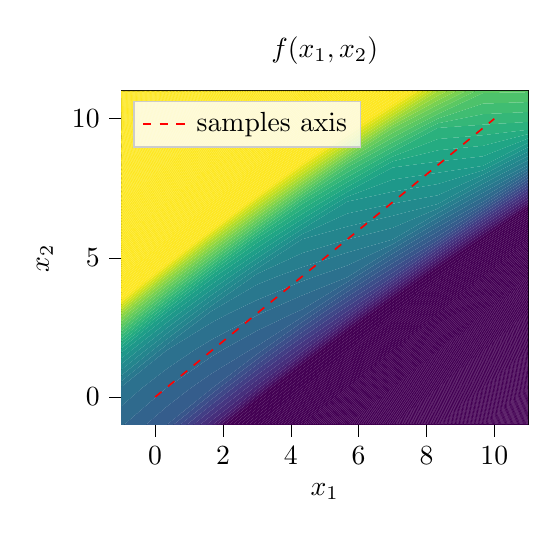
\begin{tikzpicture}

\definecolor{darkcyan30152138}{RGB}{30,152,138}
\definecolor{darkcyan30158136}{RGB}{30,158,136}
\definecolor{darkcyan32145140}{RGB}{32,145,140}
\definecolor{darkcyan34138141}{RGB}{34,138,141}
\definecolor{darkcyan36133141}{RGB}{36,133,141}
\definecolor{darkcyan39126142}{RGB}{39,126,142}
\definecolor{darkgray176}{RGB}{176,176,176}
\definecolor{darkslateblue5099141}{RGB}{50,99,141}
\definecolor{darkslateblue5393140}{RGB}{53,93,140}
\definecolor{darkslateblue5686139}{RGB}{56,86,139}
\definecolor{darkslateblue6078138}{RGB}{60,78,138}
\definecolor{darkslateblue6371136}{RGB}{63,71,136}
\definecolor{darkslateblue6662133}{RGB}{66,62,133}
\definecolor{darkslateblue6954129}{RGB}{69,54,129}
\definecolor{darkslateblue7047124}{RGB}{70,47,124}
\definecolor{darkslateblue7138118}{RGB}{71,38,118}
\definecolor{gold22822724}{RGB}{228,227,24}
\definecolor{gold24623031}{RGB}{246,230,31}
\definecolor{gold25323136}{RGB}{253,231,36}
\definecolor{greenyellow19422334}{RGB}{194,223,34}
\definecolor{greenyellow21022527}{RGB}{210,225,27}
\definecolor{indigo68184}{RGB}{68,1,84}
\definecolor{indigo70992}{RGB}{70,9,92}
\definecolor{indigo7120102}{RGB}{71,20,102}
\definecolor{indigo7229111}{RGB}{72,29,111}
\definecolor{lightgray204}{RGB}{204,204,204}
\definecolor{mediumseagreen10520491}{RGB}{105,204,91}
\definecolor{mediumseagreen32165133}{RGB}{32,165,133}
\definecolor{mediumseagreen37171129}{RGB}{37,171,129}
\definecolor{mediumseagreen43177125}{RGB}{43,177,125}
\definecolor{mediumseagreen53183120}{RGB}{53,183,120}
\definecolor{mediumseagreen64189114}{RGB}{64,189,114}
\definecolor{mediumseagreen77194107}{RGB}{77,194,107}
\definecolor{mediumseagreen9120098}{RGB}{91,200,98}
\definecolor{steelblue47106141}{RGB}{47,106,141}
\definecolor{teal41120142}{RGB}{41,120,142}
\definecolor{teal44113142}{RGB}{44,113,142}
\definecolor{yellowgreen12120981}{RGB}{121,209,81}
\definecolor{yellowgreen13921370}{RGB}{139,213,70}
\definecolor{yellowgreen15721758}{RGB}{157,217,58}
\definecolor{yellowgreen17522046}{RGB}{175,220,46}

\begin{axis}[
legend cell align={left},
legend style={
  fill opacity=0.8,
  draw opacity=1,
  text opacity=1,
  at={(0.03,0.97)},
  anchor=north west,
  draw=lightgray204
},
tick align=outside,
tick pos=left,
title={\(\displaystyle f(x_1, x_2)\)},
x grid style={darkgray176},
xlabel={\(\displaystyle x_1\)},
xmin=-1, xmax=11,
xtick style={color=black},
y grid style={darkgray176},
ylabel={\(\displaystyle x_2\)},
ymin=-1, ymax=11,
ytick style={color=black}
]
\addplot [draw=none, fill=indigo68184, forget plot]
table{%
x  y
11 -1
11 -0.997896213183731
10.997803806735 -1
11 -1
};
\addplot [draw=none, fill=indigo68184, forget plot]
table{%
x  y
11 -0.997896213183731
11 -0.964235624123422
10.9626647144949 -1
10.997803806735 -1
11 -0.997896213183731
};
\addplot [draw=none, fill=indigo68184, forget plot]
table{%
x  y
11 -0.964235624123422
11 -0.930575035063114
10.9275256222548 -1
10.9626647144949 -1
11 -0.964235624123422
};
\addplot [draw=none, fill=indigo68184, forget plot]
table{%
x  y
11 -0.930575035063114
11 -0.896914446002805
10.8923865300146 -1
10.9275256222548 -1
11 -0.930575035063114
};
\addplot [draw=none, fill=indigo68184, forget plot]
table{%
x  y
11 -0.896914446002805
11 -0.863253856942496
10.8572474377745 -1
10.8923865300146 -1
11 -0.896914446002805
};
\addplot [draw=none, fill=indigo68184, forget plot]
table{%
x  y
11 -0.863253856942496
11 -0.829593267882188
10.8221083455344 -1
10.8572474377745 -1
11 -0.863253856942496
};
\addplot [draw=none, fill=indigo68184, forget plot]
table{%
x  y
11 -0.829593267882188
11 -0.795932678821879
10.7869692532943 -1
10.8221083455344 -1
11 -0.829593267882188
};
\addplot [draw=none, fill=indigo68184, forget plot]
table{%
x  y
11 -0.795932678821879
11 -0.762272089761571
10.7518301610542 -1
10.7869692532943 -1
11 -0.795932678821879
};
\addplot [draw=none, fill=indigo68184, forget plot]
table{%
x  y
11 -0.762272089761571
11 -0.728611500701262
10.7166910688141 -1
10.7518301610542 -1
11 -0.762272089761571
};
\addplot [draw=none, fill=indigo68184, forget plot]
table{%
x  y
11 -0.728611500701262
11 -0.694950911640954
10.6815519765739 -1
10.7166910688141 -1
11 -0.728611500701262
};
\addplot [draw=none, fill=indigo68184, forget plot]
table{%
x  y
11 -0.694950911640954
11 -0.661290322580645
10.6464128843338 -1
10.6815519765739 -1
11 -0.694950911640954
};
\addplot [draw=none, fill=indigo68184, forget plot]
table{%
x  y
11 -0.661290322580645
11 -0.627629733520337
10.6112737920937 -1
10.6464128843338 -1
11 -0.661290322580645
};
\addplot [draw=none, fill=indigo68184, forget plot]
table{%
x  y
11 -0.627629733520337
11 -0.593969144460028
10.5761346998536 -1
10.6112737920937 -1
11 -0.627629733520337
};
\addplot [draw=none, fill=indigo68184, forget plot]
table{%
x  y
11 -0.593969144460028
11 -0.56030855539972
10.5409956076135 -1
10.5761346998536 -1
11 -0.593969144460028
};
\addplot [draw=none, fill=indigo68184, forget plot]
table{%
x  y
11 -0.56030855539972
11 -0.526647966339411
10.5058565153734 -1
10.5409956076135 -1
11 -0.56030855539972
};
\addplot [draw=none, fill=indigo68184, forget plot]
table{%
x  y
11 -0.526647966339411
11 -0.492987377279102
10.4707174231332 -1
10.5058565153734 -1
11 -0.526647966339411
};
\addplot [draw=none, fill=indigo68184, forget plot]
table{%
x  y
11 -0.492987377279102
11 -0.459326788218794
10.4355783308931 -1
10.4707174231332 -1
11 -0.492987377279102
};
\addplot [draw=none, fill=indigo68184, forget plot]
table{%
x  y
11 -0.459326788218794
11 -0.425666199158485
10.400439238653 -1
10.4355783308931 -1
11 -0.459326788218794
};
\addplot [draw=none, fill=indigo68184, forget plot]
table{%
x  y
11 -0.425666199158485
11 -0.392005610098177
10.3653001464129 -1
10.400439238653 -1
11 -0.425666199158485
};
\addplot [draw=none, fill=indigo68184, forget plot]
table{%
x  y
11 -0.392005610098177
11 -0.358345021037868
10.3301610541728 -1
10.3653001464129 -1
11 -0.392005610098177
};
\addplot [draw=none, fill=indigo68184, forget plot]
table{%
x  y
11 -0.358345021037868
11 -0.32468443197756
10.2950219619327 -1
10.3301610541728 -1
11 -0.358345021037868
};
\addplot [draw=none, fill=indigo68184, forget plot]
table{%
x  y
11 -0.32468443197756
11 -0.291023842917251
10.2598828696925 -1
10.2950219619327 -1
11 -0.32468443197756
};
\addplot [draw=none, fill=indigo68184, forget plot]
table{%
x  y
11 -0.291023842917251
11 -0.257363253856943
10.2247437774524 -1
10.2598828696925 -1
11 -0.291023842917251
};
\addplot [draw=none, fill=indigo68184, forget plot]
table{%
x  y
11 -0.257363253856943
11 -0.223702664796634
10.1896046852123 -1
10.2247437774524 -1
11 -0.257363253856943
};
\addplot [draw=none, fill=indigo68184, forget plot]
table{%
x  y
11 -0.223702664796634
11 -0.190042075736326
10.1544655929722 -1
10.1896046852123 -1
11 -0.223702664796634
};
\addplot [draw=none, fill=indigo68184, forget plot]
table{%
x  y
11 -0.190042075736326
11 -0.156381486676017
10.1193265007321 -1
10.1544655929722 -1
11 -0.190042075736326
};
\addplot [draw=none, fill=indigo68184, forget plot]
table{%
x  y
11 -0.156381486676017
11 -0.122720897615708
10.0841874084919 -1
10.1193265007321 -1
11 -0.156381486676017
};
\addplot [draw=none, fill=indigo68184, forget plot]
table{%
x  y
11 -0.122720897615708
11 -0.0890603085553999
10.0490483162518 -1
10.0841874084919 -1
11 -0.122720897615708
};
\addplot [draw=none, fill=indigo68184, forget plot]
table{%
x  y
11 -0.0890603085553999
11 -0.0553997194950913
10.0139092240117 -1
10.0490483162518 -1
11 -0.0890603085553999
};
\addplot [draw=none, fill=indigo68184, forget plot]
table{%
x  y
11 -0.0553997194950913
11 -0.0217391304347828
9.9787701317716 -1
10.0139092240117 -1
11 -0.0553997194950913
};
\addplot [draw=none, fill=indigo68184, forget plot]
table{%
x  y
11 -0.0217391304347828
11 0.0119214586255258
9.94363103953148 -1
9.9787701317716 -1
11 -0.0217391304347828
};
\addplot [draw=none, fill=indigo68184, forget plot]
table{%
x  y
11 0.0119214586255258
11 0.0455820476858343
9.90849194729136 -1
9.94363103953148 -1
11 0.0119214586255258
};
\addplot [draw=none, fill=indigo68184, forget plot]
table{%
x  y
11 0.0455820476858343
11 0.0792426367461429
9.87335285505124 -1
9.90849194729136 -1
11 0.0455820476858343
};
\addplot [draw=none, fill=indigo68184, forget plot]
table{%
x  y
11 0.0792426367461429
11 0.112903225806451
9.83821376281113 -1
9.87335285505124 -1
11 0.0792426367461429
};
\addplot [draw=none, fill=indigo68184, forget plot]
table{%
x  y
11 0.112903225806451
11 0.14656381486676
9.80307467057101 -1
9.83821376281113 -1
11 0.112903225806451
};
\addplot [draw=none, fill=indigo68184, forget plot]
table{%
x  y
11 0.14656381486676
11 0.180224403927069
9.76793557833089 -1
9.80307467057101 -1
11 0.14656381486676
};
\addplot [draw=none, fill=indigo68184, forget plot]
table{%
x  y
11 0.180224403927069
11 0.213884992987377
9.73279648609078 -1
9.76793557833089 -1
11 0.180224403927069
};
\addplot [draw=none, fill=indigo68184, forget plot]
table{%
x  y
11 0.213884992987377
11 0.247545582047686
9.69765739385066 -1
9.73279648609078 -1
11 0.213884992987377
};
\addplot [draw=none, fill=indigo68184, forget plot]
table{%
x  y
9.66666666666667 -1
9.69765739385066 -1
11 0.247545582047686
11 0.281206171107994
9.66666666666667 -0.995495495495495
9.66196793808734 -1
9.66666666666667 -1
};
\addplot [draw=none, fill=indigo68184, forget plot]
table{%
x  y
9.66666666666667 -0.995495495495495
11 0.281206171107994
11 0.314866760168303
9.66666666666667 -0.95733969263381
9.62216694306247 -1
9.66196793808734 -1
9.66666666666667 -0.995495495495495
};
\addplot [draw=none, fill=indigo68184, forget plot]
table{%
x  y
9.66666666666667 -0.95733969263381
11 0.314866760168303
11 0.333333333333333
11 0.350447604002106
10.9819143016138 0.333333333333333
9.66666666666667 -0.919183889772125
9.58236594803759 -1
9.62216694306247 -1
9.66666666666667 -0.95733969263381
};
\addplot [draw=none, fill=indigo68184, forget plot]
table{%
x  y
9.66666666666667 -0.919183889772125
10.9819143016138 0.333333333333333
11 0.350447604002106
11 0.388362295945234
10.9418475236505 0.333333333333333
9.66666666666667 -0.881028086910439
9.54256495301271 -1
9.58236594803759 -1
9.66666666666667 -0.919183889772125
};
\addplot [draw=none, fill=indigo68184, forget plot]
table{%
x  y
9.66666666666667 -0.881028086910439
10.9418475236505 0.333333333333333
11 0.388362295945234
11 0.426276987888362
10.9017807456873 0.333333333333333
9.66666666666666 -0.842872284048754
9.50276395798784 -1
9.54256495301271 -1
9.66666666666667 -0.881028086910439
};
\addplot [draw=none, fill=indigo68184, forget plot]
table{%
x  y
9.66666666666667 -0.842872284048754
10.9017807456873 0.333333333333333
11 0.426276987888362
11 0.46419167983149
10.861713967724 0.333333333333333
9.66666666666667 -0.804716481187069
9.46296296296296 -1
9.50276395798784 -1
9.66666666666667 -0.842872284048754
};
\addplot [draw=none, fill=indigo68184, forget plot]
table{%
x  y
9.66666666666667 -0.804716481187069
10.861713967724 0.333333333333333
11 0.46419167983149
11 0.502106371774618
10.8216471897607 0.333333333333333
9.66666666666667 -0.766560678325384
9.42316196793809 -1
9.46296296296296 -1
9.66666666666667 -0.804716481187069
};
\addplot [draw=none, fill=indigo68184, forget plot]
table{%
x  y
9.66666666666667 -0.766560678325384
10.8216471897607 0.333333333333333
11 0.502106371774618
11 0.540021063717746
10.7815804117974 0.333333333333333
9.66666666666667 -0.728404875463699
9.38336097291321 -1
9.42316196793809 -1
9.66666666666667 -0.766560678325384
};
\addplot [draw=none, fill=indigo68184, forget plot]
table{%
x  y
9.66666666666667 -0.728404875463699
10.7815804117974 0.333333333333333
11 0.540021063717746
11 0.577935755660874
10.7415136338342 0.333333333333333
9.66666666666667 -0.690249072602014
9.34355997788833 -1
9.38336097291321 -1
9.66666666666667 -0.728404875463699
};
\addplot [draw=none, fill=indigo68184, forget plot]
table{%
x  y
9.66666666666667 -0.690249072602014
10.7415136338342 0.333333333333333
11 0.577935755660874
11 0.615850447604002
10.7014468558709 0.333333333333333
9.66666666666667 -0.652093269740328
9.30375898286346 -1
9.34355997788833 -1
9.66666666666667 -0.690249072602014
};
\addplot [draw=none, fill=indigo68184, forget plot]
table{%
x  y
9.66666666666667 -0.652093269740328
10.7014468558709 0.333333333333333
11 0.615850447604002
11 0.65376513954713
10.6613800779076 0.333333333333333
9.66666666666667 -0.613937466878643
9.26395798783858 -1
9.30375898286346 -1
9.66666666666667 -0.652093269740328
};
\addplot [draw=none, fill=indigo68184, forget plot]
table{%
x  y
9.66666666666667 -0.613937466878643
10.6613800779076 0.333333333333333
11 0.65376513954713
11 0.691679831490258
10.6213132999444 0.333333333333333
9.66666666666666 -0.575781664016958
9.22415699281371 -1
9.26395798783858 -1
9.66666666666667 -0.613937466878643
};
\addplot [draw=none, fill=indigo68184, forget plot]
table{%
x  y
9.66666666666667 -0.575781664016958
10.6213132999444 0.333333333333333
11 0.691679831490258
11 0.729594523433386
10.5812465219811 0.333333333333333
9.66666666666667 -0.537625861155273
9.18435599778883 -1
9.22415699281371 -1
9.66666666666667 -0.575781664016958
};
\addplot [draw=none, fill=indigo68184, forget plot]
table{%
x  y
9.66666666666667 -0.537625861155273
10.5812465219811 0.333333333333333
11 0.729594523433386
11 0.767509215376514
10.5411797440178 0.333333333333333
9.66666666666667 -0.499470058293588
9.14455500276396 -1
9.18435599778883 -1
9.66666666666667 -0.537625861155273
};
\addplot [draw=none, fill=indigo68184, forget plot]
table{%
x  y
9.66666666666667 -0.499470058293588
10.5411797440178 0.333333333333333
11 0.767509215376514
11 0.805423907319642
10.5011129660545 0.333333333333333
9.66666666666667 -0.461314255431903
9.10475400773908 -1
9.14455500276396 -1
9.66666666666667 -0.499470058293588
};
\addplot [draw=none, fill=indigo68184, forget plot]
table{%
x  y
9.66666666666667 -0.461314255431903
10.5011129660545 0.333333333333333
11 0.805423907319642
11 0.84333859926277
10.4610461880913 0.333333333333333
9.66666666666667 -0.423158452570217
9.06495301271421 -1
9.10475400773908 -1
9.66666666666667 -0.461314255431903
};
\addplot [draw=none, fill=indigo68184, forget plot]
table{%
x  y
9.66666666666667 -0.423158452570217
10.4610461880913 0.333333333333333
11 0.84333859926277
11 0.881253291205898
10.420979410128 0.333333333333333
9.66666666666667 -0.385002649708532
9.02515201768933 -1
9.06495301271421 -1
9.66666666666667 -0.423158452570217
};
\addplot [draw=none, fill=indigo68184, forget plot]
table{%
x  y
9.66666666666667 -0.385002649708532
10.420979410128 0.333333333333333
11 0.881253291205898
11 0.919167983149026
10.3809126321647 0.333333333333333
9.66666666666667 -0.346846846846847
8.98535102266445 -1
9.02515201768933 -1
9.66666666666667 -0.385002649708532
};
\addplot [draw=none, fill=indigo68184, forget plot]
table{%
x  y
9.66666666666667 -0.346846846846847
10.3809126321647 0.333333333333333
11 0.919167983149026
11 0.957082675092154
10.3408458542014 0.333333333333333
9.66666666666667 -0.308691043985162
8.94555002763958 -1
8.98535102266445 -1
9.66666666666667 -0.346846846846847
};
\addplot [draw=none, fill=indigo68184, forget plot]
table{%
x  y
9.66666666666667 -0.308691043985162
10.3408458542014 0.333333333333333
11 0.957082675092154
11 0.994997367035282
10.3007790762382 0.333333333333333
9.66666666666667 -0.270535241123477
8.9057490326147 -1
8.94555002763958 -1
9.66666666666667 -0.308691043985162
};
\addplot [draw=none, fill=indigo68184, forget plot]
table{%
x  y
9.66666666666667 -0.270535241123477
10.3007790762382 0.333333333333333
11 0.994997367035282
11 1.03291205897841
10.2607122982749 0.333333333333333
9.66666666666667 -0.232379438261792
8.86594803758983 -1
8.9057490326147 -1
9.66666666666667 -0.270535241123477
};
\addplot [draw=none, fill=indigo68184, forget plot]
table{%
x  y
9.66666666666667 -0.232379438261792
10.2607122982749 0.333333333333333
11 1.03291205897841
11 1.07082675092154
10.2206455203116 0.333333333333333
9.66666666666667 -0.194223635400106
8.82614704256495 -1
8.86594803758983 -1
9.66666666666667 -0.232379438261792
};
\addplot [draw=none, fill=indigo68184, forget plot]
table{%
x  y
9.66666666666667 -0.194223635400106
10.2206455203116 0.333333333333333
11 1.07082675092154
11 1.10874144286467
10.1805787423484 0.333333333333333
9.66666666666667 -0.156067832538421
8.78634604754008 -1
8.82614704256495 -1
9.66666666666667 -0.194223635400106
};
\addplot [draw=none, fill=indigo68184, forget plot]
table{%
x  y
9.66666666666667 -0.156067832538421
10.1805787423484 0.333333333333333
11 1.10874144286467
11 1.14665613480779
10.1405119643851 0.333333333333333
9.66666666666667 -0.117912029676736
8.7465450525152 -1
8.78634604754008 -1
9.66666666666667 -0.156067832538421
};
\addplot [draw=none, fill=indigo68184, forget plot]
table{%
x  y
9.66666666666667 -0.117912029676736
10.1405119643851 0.333333333333333
11 1.14665613480779
11 1.18457082675092
10.1004451864218 0.333333333333333
9.66666666666667 -0.0797562268150508
8.70674405749033 -1
8.7465450525152 -1
9.66666666666667 -0.117912029676736
};
\addplot [draw=none, fill=indigo68184, forget plot]
table{%
x  y
9.66666666666666 -0.0797562268150509
10.1004451864218 0.333333333333333
11 1.18457082675092
11 1.22248551869405
10.0603784084585 0.333333333333333
9.66666666666667 -0.0416004239533657
8.66694306246545 -1
8.70674405749033 -1
9.66666666666666 -0.0797562268150509
};
\addplot [draw=none, fill=indigo68184, forget plot]
table{%
x  y
9.66666666666667 -0.0416004239533657
10.0603784084585 0.333333333333333
11 1.22248551869405
11 1.26040021063718
10.0203116304953 0.333333333333333
9.66666666666667 -0.00344462109168051
8.62714206744057 -1
8.66694306246545 -1
9.66666666666667 -0.0416004239533657
};
\addplot [draw=none, fill=indigo68184, forget plot]
table{%
x  y
9.66666666666667 -0.00344462109168051
10.0203116304953 0.333333333333333
11 1.26040021063718
11 1.29831490258031
9.980244852532 0.333333333333333
9.66666666666667 0.0347111817700047
8.5873410724157 -1
8.62714206744057 -1
9.66666666666667 -0.00344462109168051
};
\addplot [draw=none, fill=indigo68184, forget plot]
table{%
x  y
9.66666666666667 0.0347111817700047
9.980244852532 0.333333333333333
11 1.29831490258031
11 1.33622959452343
9.94017807456873 0.333333333333333
9.66666666666667 0.0728669846316898
8.54754007739082 -1
8.5873410724157 -1
9.66666666666667 0.0347111817700047
};
\addplot [draw=none, fill=indigo68184, forget plot]
table{%
x  y
9.66666666666667 0.0728669846316898
9.94017807456873 0.333333333333333
11 1.33622959452343
11 1.37414428646656
9.90011129660545 0.333333333333333
9.66666666666667 0.111022787493375
8.50773908236595 -1
8.54754007739082 -1
9.66666666666667 0.0728669846316898
};
\addplot [draw=none, fill=indigo68184, forget plot]
table{%
x  y
9.66666666666666 0.111022787493375
9.90011129660545 0.333333333333333
11 1.37414428646656
11 1.41205897840969
9.86004451864218 0.333333333333333
9.66666666666667 0.14917859035506
8.46793808734107 -1
8.50773908236595 -1
9.66666666666666 0.111022787493375
};
\addplot [draw=none, fill=indigo68184, forget plot]
table{%
x  y
9.66666666666667 0.14917859035506
9.86004451864218 0.333333333333333
11 1.41205897840969
11 1.44997367035282
9.81997774067891 0.333333333333333
9.66666666666667 0.187334393216745
8.4281370923162 -1
8.46793808734107 -1
9.66666666666667 0.14917859035506
};
\addplot [draw=none, fill=indigo68184, forget plot]
table{%
x  y
9.66666666666667 0.187334393216745
9.81997774067891 0.333333333333333
11 1.44997367035282
11 1.48788836229595
9.77991096271564 0.333333333333333
9.66666666666667 0.225490196078431
8.38833609729132 -1
8.4281370923162 -1
9.66666666666667 0.187334393216745
};
\addplot [draw=none, fill=indigo68184, forget plot]
table{%
x  y
9.66666666666667 0.22549019607843
9.77991096271564 0.333333333333333
11 1.48788836229595
11 1.52580305423907
9.73984418475236 0.333333333333333
9.66666666666667 0.263645998940116
8.34853510226645 -1
8.38833609729132 -1
9.66666666666667 0.22549019607843
};
\addplot [draw=none, fill=indigo68184, forget plot]
table{%
x  y
8.33333333333333 -1
8.34853510226645 -1
9.66666666666667 0.263645998940116
9.73984418475236 0.333333333333333
11 1.52580305423907
11 1.5637177461822
9.69977740678909 0.333333333333333
9.66666666666667 0.301801801801801
8.33333333333333 -0.972782874617738
8.30497131931166 -1
8.33333333333333 -1
};
\addplot [draw=none, fill=indigo68184, forget plot]
table{%
x  y
8.33333333333333 -0.972782874617738
9.66666666666666 0.301801801801801
9.69977740678909 0.333333333333333
11 1.5637177461822
11 1.60163243812533
9.66666666666667 0.340922890103217
9.65863840719332 0.333333333333333
8.33333333333333 -0.928746177370032
8.25908221797323 -1
8.30497131931166 -1
8.33333333333333 -0.972782874617738
};
\addplot [draw=none, fill=indigo68184, forget plot]
table{%
x  y
8.33333333333333 -0.928746177370032
9.65863840719332 0.333333333333333
9.66666666666667 0.340922890103217
11 1.60163243812533
11 1.63954713006846
9.66666666666667 0.384638737097752
9.61239563262685 0.333333333333333
8.33333333333333 -0.884709480122325
8.2131931166348 -1
8.25908221797323 -1
8.33333333333333 -0.928746177370032
};
\addplot [draw=none, fill=indigo68184, forget plot]
table{%
x  y
8.33333333333333 -0.884709480122325
9.61239563262685 0.333333333333333
9.66666666666667 0.384638737097752
11 1.63954713006846
11 1.66666666666667
11 1.67902350813743
10.9867313915858 1.66666666666667
9.66666666666667 0.428354584092288
9.56615285806037 0.333333333333333
8.33333333333333 -0.840672782874619
8.16730401529637 -1
8.2131931166348 -1
8.33333333333333 -0.884709480122325
};
\addplot [draw=none, fill=indigo68184, forget plot]
table{%
x  y
8.33333333333333 -0.840672782874619
9.56615285806037 0.333333333333333
9.66666666666667 0.428354584092288
10.9867313915858 1.66666666666667
11 1.67902350813743
11 1.72242314647378
10.9401294498382 1.66666666666667
9.66666666666667 0.472070431086823
9.5199100834939 0.333333333333333
8.33333333333333 -0.796636085626912
8.12141491395793 -1
8.16730401529637 -1
8.33333333333333 -0.840672782874619
};
\addplot [draw=none, fill=indigo68184, forget plot]
table{%
x  y
8.33333333333333 -0.796636085626912
9.5199100834939 0.333333333333333
9.66666666666667 0.472070431086823
10.9401294498382 1.66666666666667
11 1.72242314647378
11 1.76582278481013
10.8935275080906 1.66666666666667
9.66666666666667 0.515786278081359
9.47366730892742 0.333333333333333
8.33333333333333 -0.752599388379206
8.0755258126195 -1
8.12141491395793 -1
8.33333333333333 -0.796636085626912
};
\addplot [draw=none, fill=indigo68184, forget plot]
table{%
x  y
8.33333333333333 -0.752599388379206
9.47366730892742 0.333333333333333
9.66666666666667 0.515786278081359
10.8935275080906 1.66666666666667
11 1.76582278481013
11 1.80922242314647
10.846925566343 1.66666666666667
9.66666666666666 0.559502125075895
9.42742453436095 0.333333333333333
8.33333333333333 -0.7085626911315
8.02963671128107 -1
8.0755258126195 -1
8.33333333333333 -0.752599388379206
};
\addplot [draw=none, fill=indigo68184, forget plot]
table{%
x  y
8.33333333333333 -0.7085626911315
9.42742453436095 0.333333333333333
9.66666666666667 0.559502125075895
10.846925566343 1.66666666666667
11 1.80922242314647
11 1.85262206148282
10.8003236245955 1.66666666666667
9.66666666666667 0.60321797207043
9.38118175979448 0.333333333333333
8.33333333333333 -0.664525993883793
7.98374760994264 -1
8.02963671128107 -1
8.33333333333333 -0.7085626911315
};
\addplot [draw=none, fill=indigo68184, forget plot]
table{%
x  y
8.33333333333333 -0.664525993883793
9.38118175979448 0.333333333333333
9.66666666666667 0.60321797207043
10.8003236245955 1.66666666666667
11 1.85262206148282
11 1.89602169981917
10.7537216828479 1.66666666666667
9.66666666666667 0.646933819064966
9.334938985228 0.333333333333333
8.33333333333333 -0.620489296636087
7.93785850860421 -1
7.98374760994264 -1
8.33333333333333 -0.664525993883793
};
\addplot [draw=none, fill=indigo68184, forget plot]
table{%
x  y
8.33333333333333 -0.620489296636087
9.334938985228 0.333333333333333
9.66666666666667 0.646933819064966
10.7537216828479 1.66666666666667
11 1.89602169981917
11 1.93942133815552
10.7071197411003 1.66666666666667
9.66666666666666 0.690649666059501
9.28869621066153 0.333333333333333
8.33333333333333 -0.57645259938838
7.89196940726577 -1
7.93785850860421 -1
8.33333333333333 -0.620489296636087
};
\addplot [draw=none, fill=indigo68184, forget plot]
table{%
x  y
8.33333333333333 -0.57645259938838
9.28869621066153 0.333333333333333
9.66666666666667 0.690649666059501
10.7071197411003 1.66666666666667
11 1.93942133815552
11 1.98282097649186
10.6605177993527 1.66666666666667
9.66666666666667 0.734365513054037
9.24245343609505 0.333333333333333
8.33333333333333 -0.532415902140674
7.84608030592734 -1
7.89196940726577 -1
8.33333333333333 -0.57645259938838
};
\addplot [draw=none, fill=indigo68184, forget plot]
table{%
x  y
8.33333333333333 -0.532415902140674
9.24245343609505 0.333333333333333
9.66666666666667 0.734365513054037
10.6605177993527 1.66666666666667
11 1.98282097649186
11 2.02622061482821
10.6139158576052 1.66666666666667
9.66666666666666 0.778081360048572
9.19621066152858 0.333333333333333
8.33333333333333 -0.488379204892967
7.80019120458891 -1
7.84608030592734 -1
8.33333333333333 -0.532415902140674
};
\addplot [draw=none, fill=indigo68184, forget plot]
table{%
x  y
8.33333333333333 -0.488379204892967
9.19621066152858 0.333333333333333
9.66666666666667 0.778081360048572
10.6139158576052 1.66666666666667
11 2.02622061482821
11 2.06962025316456
10.5673139158576 1.66666666666667
9.66666666666667 0.821797207043108
9.14996788696211 0.333333333333333
8.33333333333333 -0.444342507645261
7.75430210325048 -1
7.80019120458891 -1
8.33333333333333 -0.488379204892967
};
\addplot [draw=none, fill=indigo68184, forget plot]
table{%
x  y
8.33333333333333 -0.444342507645261
9.14996788696211 0.333333333333333
9.66666666666667 0.821797207043108
10.5673139158576 1.66666666666667
11 2.06962025316456
11 2.1130198915009
10.52071197411 1.66666666666667
9.66666666666666 0.865513054037643
9.10372511239563 0.333333333333333
8.33333333333333 -0.400305810397555
7.70841300191205 -1
7.75430210325048 -1
8.33333333333333 -0.444342507645261
};
\addplot [draw=none, fill=indigo68184, forget plot]
table{%
x  y
8.33333333333333 -0.400305810397555
9.10372511239563 0.333333333333333
9.66666666666667 0.865513054037643
10.52071197411 1.66666666666667
11 2.1130198915009
11 2.15641952983725
10.4741100323625 1.66666666666667
9.66666666666666 0.909228901032179
9.05748233782916 0.333333333333333
8.33333333333333 -0.356269113149848
7.66252390057361 -1
7.70841300191205 -1
8.33333333333333 -0.400305810397555
};
\addplot [draw=none, fill=indigo68184, forget plot]
table{%
x  y
8.33333333333333 -0.356269113149848
9.05748233782916 0.333333333333333
9.66666666666667 0.909228901032179
10.4741100323625 1.66666666666667
11 2.15641952983725
11 2.1998191681736
10.4275080906149 1.66666666666667
9.66666666666666 0.952944748026715
9.01123956326268 0.333333333333333
8.33333333333333 -0.312232415902142
7.61663479923518 -1
7.66252390057361 -1
8.33333333333333 -0.356269113149848
};
\addplot [draw=none, fill=indigo68184, forget plot]
table{%
x  y
8.33333333333333 -0.312232415902142
9.01123956326268 0.333333333333333
9.66666666666667 0.952944748026714
10.4275080906149 1.66666666666667
11 2.1998191681736
11 2.24321880650995
10.3809061488673 1.66666666666667
9.66666666666666 0.99666059502125
8.96499678869621 0.333333333333333
8.33333333333333 -0.268195718654435
7.57074569789675 -1
7.61663479923518 -1
8.33333333333333 -0.312232415902142
};
\addplot [draw=none, fill=indigo68184, forget plot]
table{%
x  y
8.33333333333333 -0.268195718654435
8.96499678869621 0.333333333333333
9.66666666666667 0.99666059502125
10.3809061488673 1.66666666666667
11 2.24321880650995
11 2.28661844484629
10.3343042071197 1.66666666666667
9.66666666666667 1.04037644201579
8.91875401412974 0.333333333333333
8.33333333333333 -0.224159021406729
7.52485659655832 -1
7.57074569789675 -1
8.33333333333333 -0.268195718654435
};
\addplot [draw=none, fill=indigo68184, forget plot]
table{%
x  y
8.33333333333333 -0.224159021406729
8.91875401412974 0.333333333333333
9.66666666666667 1.04037644201579
10.3343042071197 1.66666666666667
11 2.28661844484629
11 2.33001808318264
10.2877022653722 1.66666666666667
9.66666666666667 1.08409228901032
8.87251123956326 0.333333333333333
8.33333333333333 -0.180122324159023
7.47896749521989 -1
7.52485659655832 -1
8.33333333333333 -0.224159021406729
};
\addplot [draw=none, fill=indigo68184, forget plot]
table{%
x  y
8.33333333333333 -0.180122324159022
8.87251123956326 0.333333333333333
9.66666666666667 1.08409228901032
10.2877022653722 1.66666666666667
11 2.33001808318264
11 2.37341772151899
10.2411003236246 1.66666666666667
9.66666666666667 1.12780813600486
8.82626846499679 0.333333333333333
8.33333333333333 -0.136085626911316
7.43307839388145 -1
7.47896749521989 -1
8.33333333333333 -0.180122324159022
};
\addplot [draw=none, fill=indigo68184, forget plot]
table{%
x  y
8.33333333333333 -0.136085626911316
8.82626846499679 0.333333333333333
9.66666666666667 1.12780813600486
10.2411003236246 1.66666666666667
11 2.37341772151899
11 2.41681735985533
10.194498381877 1.66666666666667
9.66666666666667 1.17152398299939
8.78002569043031 0.333333333333333
8.33333333333333 -0.0920489296636095
7.38718929254302 -1
7.43307839388145 -1
8.33333333333333 -0.136085626911316
};
\addplot [draw=none, fill=indigo68184, forget plot]
table{%
x  y
8.33333333333333 -0.0920489296636096
8.78002569043031 0.333333333333333
9.66666666666667 1.17152398299939
10.194498381877 1.66666666666667
11 2.41681735985533
11 2.46021699819168
10.1478964401294 1.66666666666667
9.66666666666667 1.21523982999393
8.73378291586384 0.333333333333333
8.33333333333333 -0.0480122324159031
7.34130019120459 -1
7.38718929254302 -1
8.33333333333333 -0.0920489296636096
};
\addplot [draw=none, fill=indigo68184, forget plot]
table{%
x  y
8.33333333333333 -0.0480122324159032
8.73378291586384 0.333333333333333
9.66666666666667 1.21523982999393
10.1478964401294 1.66666666666667
11 2.46021699819168
11 2.50361663652803
10.1012944983819 1.66666666666667
9.66666666666667 1.25895567698846
8.68754014129737 0.333333333333333
8.33333333333333 -0.00397553516819668
7.29541108986616 -1
7.34130019120459 -1
8.33333333333333 -0.0480122324159032
};
\addplot [draw=none, fill=indigo68184, forget plot]
table{%
x  y
8.33333333333333 -0.00397553516819679
8.68754014129737 0.333333333333333
9.66666666666667 1.25895567698846
10.1012944983819 1.66666666666667
11 2.50361663652803
11 2.54701627486438
10.0546925566343 1.66666666666667
9.66666666666667 1.302671523983
8.64129736673089 0.333333333333333
8.33333333333333 0.0400611620795097
7.24952198852773 -1
7.29541108986616 -1
8.33333333333333 -0.00397553516819679
};
\addplot [draw=none, fill=indigo68184, forget plot]
table{%
x  y
8.33333333333333 0.0400611620795097
8.64129736673089 0.333333333333333
9.66666666666667 1.302671523983
10.0546925566343 1.66666666666667
11 2.54701627486438
11 2.59041591320072
10.0080906148867 1.66666666666667
9.66666666666667 1.34638737097753
8.59505459216442 0.333333333333333
8.33333333333333 0.0840978593272161
7.20363288718929 -1
7.24952198852773 -1
8.33333333333333 0.0400611620795097
};
\addplot [draw=none, fill=indigo68184, forget plot]
table{%
x  y
8.33333333333333 0.0840978593272161
8.59505459216442 0.333333333333333
9.66666666666667 1.34638737097753
10.0080906148867 1.66666666666667
11 2.59041591320072
11 2.63381555153707
9.96148867313916 1.66666666666667
9.66666666666667 1.39010321797207
8.54881181759795 0.333333333333333
8.33333333333333 0.128134556574923
7.15774378585086 -1
7.20363288718929 -1
8.33333333333333 0.0840978593272161
};
\addplot [draw=none, fill=indigo68184, forget plot]
table{%
x  y
8.33333333333333 0.128134556574923
8.54881181759794 0.333333333333333
9.66666666666667 1.39010321797207
9.96148867313916 1.66666666666667
11 2.63381555153707
11 2.67721518987342
9.91488673139158 1.66666666666667
9.66666666666667 1.43381906496661
8.50256904303147 0.333333333333333
8.33333333333333 0.172171253822629
7.11185468451243 -1
7.15774378585086 -1
8.33333333333333 0.128134556574923
};
\addplot [draw=none, fill=indigo68184, forget plot]
table{%
x  y
8.33333333333333 0.172171253822629
8.50256904303147 0.333333333333333
9.66666666666667 1.43381906496661
9.91488673139158 1.66666666666667
11 2.67721518987342
11 2.72061482820977
9.86828478964401 1.66666666666667
9.66666666666667 1.47753491196114
8.456326268465 0.333333333333333
8.33333333333333 0.216207951070335
7.065965583174 -1
7.11185468451243 -1
8.33333333333333 0.172171253822629
};
\addplot [draw=none, fill=indigo68184, forget plot]
table{%
x  y
8.33333333333333 0.216207951070335
8.456326268465 0.333333333333333
9.66666666666667 1.47753491196114
9.86828478964401 1.66666666666667
11 2.72061482820977
11 2.76401446654611
9.82168284789644 1.66666666666667
9.66666666666667 1.52125075895568
8.41008349389852 0.333333333333333
8.33333333333333 0.260244648318042
7.02007648183556 -1
7.065965583174 -1
8.33333333333333 0.216207951070335
};
\addplot [draw=none, fill=indigo68184, forget plot]
table{%
x  y
7 -1
7.02007648183556 -1
8.33333333333333 0.260244648318042
8.41008349389852 0.333333333333333
9.66666666666667 1.52125075895568
9.82168284789644 1.66666666666667
11 2.76401446654611
11 2.80741410488246
9.77508090614887 1.66666666666667
9.66666666666667 1.56496660595021
8.36384071933205 0.333333333333333
8.33333333333333 0.304281345565748
7 -0.970715835140998
6.96952595936795 -1
7 -1
};
\addplot [draw=none, fill=indigo68184, forget plot]
table{%
x  y
7 -0.970715835140998
8.33333333333333 0.304281345565748
8.36384071933205 0.333333333333333
9.66666666666667 1.56496660595021
9.77508090614887 1.66666666666667
11 2.80741410488246
11 2.85081374321881
9.72847896440129 1.66666666666667
9.66666666666667 1.60868245294475
8.33333333333333 0.350896057347669
8.31473044798785 0.333333333333333
7 -0.918655097613883
6.91534988713318 -1
6.96952595936795 -1
7 -0.970715835140998
};
\addplot [draw=none, fill=indigo68184, forget plot]
table{%
x  y
7 -0.918655097613883
8.31473044798785 0.333333333333333
8.33333333333333 0.350896057347669
9.66666666666667 1.60868245294475
9.72847896440129 1.66666666666667
11 2.85081374321881
11 2.89421338155515
9.68187702265372 1.66666666666667
9.66666666666667 1.65239829993928
8.33333333333333 0.402508960573476
8.26006074411541 0.333333333333333
7 -0.866594360086768
6.86117381489842 -1
6.91534988713318 -1
7 -0.918655097613883
};
\addplot [draw=none, fill=indigo68184, forget plot]
table{%
x  y
7 -0.866594360086768
8.26006074411541 0.333333333333333
8.33333333333333 0.402508960573476
9.66666666666667 1.65239829993928
9.68187702265372 1.66666666666667
11 2.89421338155515
11 2.9376130198915
9.66666666666667 1.70113717128642
9.62950191570881 1.66666666666667
8.33333333333333 0.454121863799282
8.20539104024298 0.333333333333333
7 -0.814533622559653
6.80699774266366 -1
6.86117381489842 -1
7 -0.866594360086768
};
\addplot [draw=none, fill=indigo68184, forget plot]
table{%
x  y
7 -0.814533622559653
8.20539104024298 0.333333333333333
8.33333333333333 0.454121863799282
9.62950191570881 1.66666666666667
9.66666666666667 1.70113717128642
11 2.9376130198915
11 2.98101265822785
9.66666666666667 1.75230987917555
9.57432950191571 1.66666666666667
8.33333333333333 0.505734767025088
8.15072133637054 0.333333333333333
7 -0.762472885032538
6.75282167042889 -1
6.80699774266366 -1
7 -0.814533622559653
};
\addplot [draw=none, fill=indigo68184, forget plot]
table{%
x  y
7 -0.762472885032538
8.15072133637054 0.333333333333333
8.33333333333333 0.505734767025088
9.57432950191571 1.66666666666667
9.66666666666667 1.75230987917555
11 2.98101265822785
11 3
11 3.02854122621564
10.9686774941995 3
9.66666666666667 1.80348258706468
9.5191570881226 1.66666666666667
8.33333333333333 0.557347670250895
8.0960516324981 0.333333333333333
7 -0.710412147505423
6.69864559819413 -1
6.75282167042889 -1
7 -0.762472885032538
};
\addplot [draw=none, fill=indigo68184, forget plot]
table{%
x  y
7 -0.710412147505423
8.0960516324981 0.333333333333333
8.33333333333333 0.557347670250895
9.5191570881226 1.66666666666667
9.66666666666667 1.80348258706468
10.9686774941995 3
11 3.02854122621564
11 3.07928118393235
10.9129930394432 3
9.66666666666667 1.8546552949538
9.4639846743295 1.66666666666667
8.33333333333333 0.608960573476701
8.04138192862566 0.333333333333333
7 -0.658351409978308
6.64446952595937 -1
6.69864559819413 -1
7 -0.710412147505423
};
\addplot [draw=none, fill=indigo68184, forget plot]
table{%
x  y
7 -0.658351409978308
8.04138192862566 0.333333333333333
8.33333333333333 0.608960573476701
9.4639846743295 1.66666666666667
9.66666666666667 1.8546552949538
10.9129930394432 3
11 3.07928118393235
11 3.13002114164905
10.8573085846868 3
9.66666666666667 1.90582800284293
9.4088122605364 1.66666666666667
8.33333333333333 0.660573476702508
7.98671222475323 0.333333333333333
7 -0.606290672451193
6.5902934537246 -1
6.64446952595937 -1
7 -0.658351409978308
};
\addplot [draw=none, fill=indigo68184, forget plot]
table{%
x  y
7 -0.606290672451193
7.98671222475323 0.333333333333333
8.33333333333333 0.660573476702508
9.4088122605364 1.66666666666667
9.66666666666667 1.90582800284293
10.8573085846868 3
11 3.13002114164905
11 3.18076109936575
10.8016241299304 3
9.66666666666667 1.95700071073205
9.35363984674329 1.66666666666667
8.33333333333333 0.712186379928314
7.93204252088079 0.333333333333333
7 -0.554229934924078
6.53611738148984 -1
6.5902934537246 -1
7 -0.606290672451193
};
\addplot [draw=none, fill=indigo68184, forget plot]
table{%
x  y
7 -0.554229934924078
7.93204252088079 0.333333333333333
8.33333333333333 0.712186379928314
9.3536398467433 1.66666666666667
9.66666666666667 1.95700071073205
10.8016241299304 3
11 3.18076109936575
11 3.23150105708245
10.745939675174 3
9.66666666666667 2.00817341862118
9.29846743295019 1.66666666666667
8.33333333333333 0.763799283154121
7.87737281700835 0.333333333333333
7 -0.502169197396963
6.48194130925508 -1
6.53611738148984 -1
7 -0.554229934924078
};
\addplot [draw=none, fill=indigo68184, forget plot]
table{%
x  y
7 -0.502169197396963
7.87737281700835 0.333333333333333
8.33333333333333 0.763799283154121
9.29846743295019 1.66666666666667
9.66666666666667 2.00817341862118
10.745939675174 3
11 3.23150105708245
11 3.28224101479915
10.6902552204176 3
9.66666666666667 2.05934612651031
9.24329501915709 1.66666666666667
8.33333333333333 0.815412186379927
7.82270311313592 0.333333333333333
7 -0.450108459869848
6.42776523702032 -1
6.48194130925508 -1
7 -0.502169197396963
};
\addplot [draw=none, fill=indigo68184, forget plot]
table{%
x  y
7 -0.450108459869848
7.82270311313591 0.333333333333333
8.33333333333333 0.815412186379927
9.24329501915709 1.66666666666667
9.66666666666667 2.05934612651031
10.6902552204176 3
11 3.28224101479915
11 3.33298097251586
10.6345707656613 3
9.66666666666667 2.11051883439943
9.18812260536398 1.66666666666667
8.33333333333333 0.867025089605734
7.76803340926348 0.333333333333333
7 -0.398047722342733
6.37358916478555 -1
6.42776523702032 -1
7 -0.450108459869848
};
\addplot [draw=none, fill=indigo68184, forget plot]
table{%
x  y
7 -0.398047722342733
7.76803340926348 0.333333333333333
8.33333333333333 0.867025089605734
9.18812260536398 1.66666666666667
9.66666666666667 2.11051883439943
10.6345707656613 3
11 3.33298097251586
11 3.38372093023256
10.5788863109049 3
9.66666666666666 2.16169154228856
9.13295019157088 1.66666666666667
8.33333333333333 0.91863799283154
7.71336370539104 0.333333333333333
7 -0.345986984815618
6.31941309255079 -1
6.37358916478555 -1
7 -0.398047722342733
};
\addplot [draw=none, fill=indigo68184, forget plot]
table{%
x  y
7 -0.345986984815618
7.71336370539104 0.333333333333333
8.33333333333333 0.91863799283154
9.13295019157088 1.66666666666667
9.66666666666667 2.16169154228856
10.5788863109049 3
11 3.38372093023256
11 3.43446088794926
10.5232018561485 3
9.66666666666667 2.21286425017768
9.07777777777778 1.66666666666667
8.33333333333333 0.970250896057347
7.6586940015186 0.333333333333333
7 -0.293926247288503
6.26523702031603 -1
6.31941309255079 -1
7 -0.345986984815618
};
\addplot [draw=none, fill=indigo68184, forget plot]
table{%
x  y
7 -0.293926247288503
7.6586940015186 0.333333333333333
8.33333333333333 0.970250896057347
9.07777777777778 1.66666666666667
9.66666666666667 2.21286425017768
10.5232018561485 3
11 3.43446088794926
11 3.48520084566596
10.4675174013921 3
9.66666666666667 2.26403695806681
9.02260536398467 1.66666666666667
8.33333333333333 1.02186379928315
7.60402429764616 0.333333333333333
7 -0.241865509761388
6.21106094808126 -1
6.26523702031603 -1
7 -0.293926247288503
};
\addplot [draw=none, fill=indigo68184, forget plot]
table{%
x  y
7 -0.241865509761388
7.60402429764616 0.333333333333333
8.33333333333333 1.02186379928315
9.02260536398467 1.66666666666667
9.66666666666667 2.26403695806681
10.4675174013921 3
11 3.48520084566596
11 3.53594080338266
10.4118329466357 3
9.66666666666667 2.31520966595593
8.96743295019157 1.66666666666667
8.33333333333333 1.07347670250896
7.54935459377373 0.333333333333333
7 -0.189804772234273
6.1568848758465 -1
6.21106094808126 -1
7 -0.241865509761388
};
\addplot [draw=none, fill=indigo68184, forget plot]
table{%
x  y
7 -0.189804772234273
7.54935459377373 0.333333333333333
8.33333333333333 1.07347670250896
8.96743295019157 1.66666666666667
9.66666666666667 2.31520966595593
10.4118329466357 3
11 3.53594080338266
11 3.58668076109937
10.3561484918794 3
9.66666666666667 2.36638237384506
8.91226053639847 1.66666666666667
8.33333333333333 1.12508960573477
7.49468488990129 0.333333333333333
7 -0.137744034707158
6.10270880361174 -1
6.1568848758465 -1
7 -0.189804772234273
};
\addplot [draw=none, fill=indigo68184, forget plot]
table{%
x  y
7 -0.137744034707158
7.49468488990129 0.333333333333333
8.33333333333333 1.12508960573477
8.91226053639847 1.66666666666667
9.66666666666667 2.36638237384506
10.3561484918794 3
11 3.58668076109937
11 3.63742071881607
10.300464037123 3
9.66666666666667 2.41755508173419
8.85708812260536 1.66666666666667
8.33333333333333 1.17670250896057
7.44001518602885 0.333333333333333
7 -0.0856832971800431
6.04853273137697 -1
6.10270880361174 -1
7 -0.137744034707158
};
\addplot [draw=none, fill=indigo68184, forget plot]
table{%
x  y
7 -0.085683297180043
7.44001518602885 0.333333333333333
8.33333333333333 1.17670250896057
8.85708812260536 1.66666666666667
9.66666666666667 2.41755508173419
10.300464037123 3
11 3.63742071881607
11 3.68816067653277
10.2447795823666 3
9.66666666666667 2.46872778962331
8.80191570881226 1.66666666666667
8.33333333333333 1.22831541218638
7.38534548215642 0.333333333333333
7 -0.033622559652928
5.99435665914221 -1
6.04853273137697 -1
7 -0.085683297180043
};
\addplot [draw=none, fill=indigo68184, forget plot]
table{%
x  y
7 -0.033622559652928
7.38534548215642 0.333333333333333
8.33333333333333 1.22831541218638
8.80191570881226 1.66666666666667
9.66666666666667 2.46872778962331
10.2447795823666 3
11 3.68816067653277
11 3.73890063424947
10.1890951276102 3
9.66666666666667 2.51990049751244
8.74674329501916 1.66666666666667
8.33333333333333 1.27992831541219
7.33067577828398 0.333333333333333
7 0.0184381778741869
5.94018058690745 -1
5.99435665914221 -1
7 -0.033622559652928
};
\addplot [draw=none, fill=indigo68184, forget plot]
table{%
x  y
7 0.0184381778741869
7.33067577828398 0.333333333333333
8.33333333333333 1.27992831541219
8.74674329501916 1.66666666666667
9.66666666666667 2.51990049751244
10.1890951276102 3
11 3.73890063424947
11 3.78964059196617
10.1334106728538 3
9.66666666666667 2.57107320540156
8.69157088122605 1.66666666666667
8.33333333333333 1.33154121863799
7.27600607441154 0.333333333333333
7 0.070498915401302
5.88600451467269 -1
5.94018058690745 -1
7 0.0184381778741869
};
\addplot [draw=none, fill=indigo68184, forget plot]
table{%
x  y
7 0.0704989154013019
7.27600607441154 0.333333333333333
8.33333333333333 1.33154121863799
8.69157088122605 1.66666666666667
9.66666666666667 2.57107320540156
10.1334106728538 3
11 3.78964059196617
11 3.84038054968288
10.0777262180974 3
9.66666666666667 2.62224591329069
8.63639846743295 1.66666666666667
8.33333333333333 1.3831541218638
7.2213363705391 0.333333333333333
7 0.122559652928417
5.83182844243792 -1
5.88600451467269 -1
7 0.0704989154013019
};
\addplot [draw=none, fill=indigo68184, forget plot]
table{%
x  y
7 0.122559652928417
7.2213363705391 0.333333333333333
8.33333333333333 1.3831541218638
8.63639846743295 1.66666666666667
9.66666666666667 2.62224591329069
10.0777262180974 3
11 3.84038054968288
11 3.89112050739958
10.0220417633411 3
9.66666666666667 2.67341862117981
8.58122605363985 1.66666666666667
8.33333333333333 1.4347670250896
7.16666666666667 0.333333333333333
7 0.174620390455532
5.77765237020316 -1
5.83182844243792 -1
7 0.122559652928417
};
\addplot [draw=none, fill=indigo68184, forget plot]
table{%
x  y
7 0.174620390455532
7.16666666666667 0.333333333333333
8.33333333333333 1.4347670250896
8.58122605363985 1.66666666666667
9.66666666666666 2.67341862117981
10.0220417633411 3
11 3.89112050739958
11 3.94186046511628
9.96635730858469 3
9.66666666666667 2.72459132906894
8.52605363984674 1.66666666666667
8.33333333333333 1.48637992831541
7.11199696279423 0.333333333333333
7 0.226681127982647
5.7234762979684 -1
5.77765237020316 -1
7 0.174620390455532
};
\addplot [draw=none, fill=indigo68184, forget plot]
table{%
x  y
7 0.226681127982647
7.11199696279423 0.333333333333333
8.33333333333333 1.48637992831541
8.52605363984674 1.66666666666667
9.66666666666667 2.72459132906894
9.96635730858469 3
11 3.94186046511628
11 3.99260042283298
9.91067285382831 3
9.66666666666667 2.77576403695807
8.47088122605364 1.66666666666667
8.33333333333333 1.53799283154122
7.05732725892179 0.333333333333333
7 0.278741865509762
5.66930022573363 -1
5.7234762979684 -1
7 0.226681127982647
};
\addplot [draw=none, fill=indigo68184, forget plot]
table{%
x  y
5.66666666666667 -1
5.66930022573363 -1
7 0.278741865509762
7.05732725892179 0.333333333333333
8.33333333333333 1.53799283154122
8.47088122605364 1.66666666666667
9.66666666666666 2.77576403695807
9.91067285382831 3
11 3.99260042283298
11 4.04334038054968
9.85498839907192 3
9.66666666666667 2.82693674484719
8.41570881226054 1.66666666666667
8.33333333333333 1.58960573476702
7.00265755504935 0.333333333333333
7 0.330802603036877
5.66666666666667 -0.939434129089302
5.60376492194674 -1
5.66666666666667 -1
};
\addplot [draw=none, fill=indigo68184, forget plot]
table{%
x  y
5.66666666666667 -0.939434129089302
7 0.330802603036877
7.00265755504935 0.333333333333333
8.33333333333333 1.58960573476702
8.41570881226054 1.66666666666667
9.66666666666667 2.82693674484719
9.85498839907192 3
11 4.04334038054968
11 4.09408033826638
9.79930394431554 3
9.66666666666667 2.87810945273632
8.36053639846743 1.66666666666667
8.33333333333333 1.64121863799283
7 0.39326334208224
6.9363974001857 0.333333333333333
5.66666666666667 -0.875773651635721
5.5376492194674 -1
5.60376492194674 -1
5.66666666666667 -0.939434129089302
};
\addplot [draw=none, fill=indigo68184, forget plot]
table{%
x  y
5.66666666666667 -0.875773651635721
6.9363974001857 0.333333333333333
7 0.39326334208224
8.33333333333333 1.64121863799283
8.36053639846743 1.66666666666667
9.66666666666667 2.87810945273632
9.79930394431554 3
11 4.09408033826638
11 4.14482029598309
9.74361948955917 3
9.66666666666667 2.92928216062544
8.33333333333333 1.6982683982684
8.29906103286385 1.66666666666667
7 0.456255468066492
6.86954503249768 0.333333333333333
5.66666666666667 -0.81211317418214
5.47153351698806 -1
5.5376492194674 -1
5.66666666666667 -0.875773651635721
};
\addplot [draw=none, fill=indigo68184, forget plot]
table{%
x  y
5.66666666666667 -0.81211317418214
6.86954503249768 0.333333333333333
7 0.456255468066492
8.29906103286385 1.66666666666667
8.33333333333333 1.6982683982684
9.66666666666667 2.92928216062544
9.74361948955917 3
11 4.14482029598309
11 4.19556025369979
9.68793503480278 3
9.66666666666667 2.98045486851457
8.33333333333333 1.76060606060606
8.23145539906103 1.66666666666667
7 0.519247594050744
6.80269266480966 0.333333333333333
5.66666666666667 -0.748452696728559
5.40541781450872 -1
5.47153351698806 -1
5.66666666666667 -0.81211317418214
};
\addplot [draw=none, fill=indigo68184, forget plot]
table{%
x  y
5.66666666666667 -0.748452696728559
6.80269266480966 0.333333333333333
7 0.519247594050744
8.23145539906103 1.66666666666667
8.33333333333333 1.76060606060606
9.66666666666667 2.98045486851457
9.68793503480278 3
11 4.19556025369979
11 4.24630021141649
9.66666666666667 3.03813196229649
9.62440645773979 3
8.33333333333333 1.82294372294372
8.16384976525822 1.66666666666667
7 0.582239720034996
6.73584029712163 0.333333333333333
5.66666666666667 -0.684792219274978
5.33930211202938 -1
5.40541781450872 -1
5.66666666666667 -0.748452696728559
};
\addplot [draw=none, fill=indigo68184, forget plot]
table{%
x  y
5.66666666666667 -0.684792219274978
6.73584029712163 0.333333333333333
7 0.582239720034996
8.16384976525822 1.66666666666667
8.33333333333333 1.82294372294372
9.62440645773979 3
9.66666666666667 3.03813196229649
11 4.24630021141649
11 4.29704016913319
9.66666666666667 3.09982862039417
9.55603038936372 3
8.33333333333333 1.88528138528138
8.0962441314554 1.66666666666667
7 0.645231846019248
6.66898792943361 0.333333333333333
5.66666666666667 -0.621131741821398
5.27318640955005 -1
5.33930211202938 -1
5.66666666666667 -0.684792219274978
};
\addplot [draw=none, fill=indigo68184, forget plot]
table{%
x  y
5.66666666666667 -0.621131741821398
6.66898792943361 0.333333333333333
7 0.645231846019248
8.0962441314554 1.66666666666667
8.33333333333333 1.88528138528138
9.55603038936372 3
9.66666666666667 3.09982862039417
11 4.29704016913319
11 4.33333333333333
11 4.35072094995759
10.9803073967339 4.33333333333333
9.66666666666667 3.16152527849186
9.48765432098766 3
8.33333333333333 1.94761904761905
8.02863849765258 1.66666666666667
7 0.7082239720035
6.60213556174559 0.333333333333333
5.66666666666667 -0.557471264367817
5.20707070707071 -1
5.27318640955005 -1
5.66666666666667 -0.621131741821398
};
\addplot [draw=none, fill=indigo68184, forget plot]
table{%
x  y
5.66666666666667 -0.557471264367817
6.60213556174559 0.333333333333333
7 0.7082239720035
8.02863849765258 1.66666666666667
8.33333333333333 1.94761904761905
9.48765432098766 3
9.66666666666667 3.16152527849186
10.9803073967339 4.33333333333333
11 4.35072094995759
11 4.41178965224767
10.9111431316042 4.33333333333333
9.66666666666667 3.22322193658955
9.41927825261159 3
8.33333333333333 2.00995670995671
7.96103286384977 1.66666666666667
7 0.771216097987752
6.53528319405757 0.333333333333333
5.66666666666667 -0.493810786914236
5.14095500459137 -1
5.20707070707071 -1
5.66666666666667 -0.557471264367817
};
\addplot [draw=none, fill=indigo68184, forget plot]
table{%
x  y
5.66666666666667 -0.493810786914236
6.53528319405757 0.333333333333333
7 0.771216097987752
7.96103286384977 1.66666666666667
8.33333333333333 2.00995670995671
9.41927825261159 3
9.66666666666667 3.22322193658955
10.9111431316042 4.33333333333333
11 4.41178965224767
11 4.47285835453774
10.8419788664745 4.33333333333333
9.66666666666667 3.28491859468723
9.35090218423552 3
8.33333333333333 2.07229437229437
7.89342723004695 1.66666666666667
7 0.834208223972004
6.46843082636954 0.333333333333333
5.66666666666667 -0.430150309460655
5.07483930211203 -1
5.14095500459137 -1
5.66666666666667 -0.493810786914236
};
\addplot [draw=none, fill=indigo68184, forget plot]
table{%
x  y
5.66666666666667 -0.430150309460655
6.46843082636954 0.333333333333333
7 0.834208223972004
7.89342723004695 1.66666666666667
8.33333333333333 2.07229437229437
9.35090218423552 3
9.66666666666667 3.28491859468723
10.8419788664745 4.33333333333333
11 4.47285835453774
11 4.53392705682782
10.7728146013449 4.33333333333333
9.66666666666667 3.34661525278492
9.28252611585945 3
8.33333333333333 2.13463203463203
7.82582159624413 1.66666666666667
7 0.897200349956256
6.40157845868152 0.333333333333333
5.66666666666667 -0.366489832007074
5.00872359963269 -1
5.07483930211203 -1
5.66666666666667 -0.430150309460655
};
\addplot [draw=none, fill=indigo68184, forget plot]
table{%
x  y
5.66666666666667 -0.366489832007074
6.40157845868152 0.333333333333333
7 0.897200349956256
7.82582159624413 1.66666666666667
8.33333333333333 2.13463203463203
9.28252611585945 3
9.66666666666667 3.34661525278492
10.7728146013449 4.33333333333333
11 4.53392705682782
11 4.5949957591179
10.7036503362152 4.33333333333333
9.66666666666667 3.4083119108826
9.21415004748338 3
8.33333333333333 2.1969696969697
7.75821596244131 1.66666666666667
7 0.960192475940508
6.3347260909935 0.333333333333333
5.66666666666667 -0.302829354553493
4.94260789715335 -1
5.00872359963269 -1
5.66666666666667 -0.366489832007074
};
\addplot [draw=none, fill=indigo68184, forget plot]
table{%
x  y
5.66666666666667 -0.302829354553493
6.3347260909935 0.333333333333333
7 0.960192475940508
7.75821596244131 1.66666666666667
8.33333333333333 2.1969696969697
9.21415004748338 3
9.66666666666667 3.4083119108826
10.7036503362152 4.33333333333333
11 4.5949957591179
11 4.65606446140797
10.6344860710855 4.33333333333333
9.66666666666667 3.47000856898029
9.14577397910731 3
8.33333333333333 2.25930735930736
7.6906103286385 1.66666666666667
7 1.02318460192476
6.26787372330548 0.333333333333333
5.66666666666667 -0.239168877099912
4.87649219467401 -1
4.94260789715335 -1
5.66666666666667 -0.302829354553493
};
\addplot [draw=none, fill=indigo68184, forget plot]
table{%
x  y
5.66666666666667 -0.239168877099912
6.26787372330548 0.333333333333333
7 1.02318460192476
7.6906103286385 1.66666666666667
8.33333333333333 2.25930735930736
9.14577397910731 3
9.66666666666667 3.47000856898029
10.6344860710855 4.33333333333333
11 4.65606446140797
11 4.71713316369805
10.5653218059558 4.33333333333333
9.66666666666667 3.53170522707798
9.07739791073124 3
8.33333333333333 2.32164502164502
7.62300469483568 1.66666666666667
7 1.08617672790901
6.20102135561746 0.333333333333333
5.66666666666667 -0.175508399646331
4.81037649219467 -1
4.87649219467401 -1
5.66666666666667 -0.239168877099912
};
\addplot [draw=none, fill=indigo68184, forget plot]
table{%
x  y
5.66666666666667 -0.175508399646331
6.20102135561746 0.333333333333333
7 1.08617672790901
7.62300469483568 1.66666666666667
8.33333333333333 2.32164502164502
9.07739791073124 3
9.66666666666667 3.53170522707798
10.5653218059558 4.33333333333333
11 4.71713316369805
11 4.77820186598812
10.4961575408261 4.33333333333333
9.66666666666667 3.59340188517566
9.00902184235517 3
8.33333333333333 2.38398268398268
7.55539906103286 1.66666666666667
7 1.14916885389326
6.13416898792943 0.333333333333333
5.66666666666667 -0.11184792219275
4.74426078971534 -1
4.81037649219467 -1
5.66666666666667 -0.175508399646331
};
\addplot [draw=none, fill=indigo68184, forget plot]
table{%
x  y
5.66666666666667 -0.11184792219275
6.13416898792943 0.333333333333333
7 1.14916885389326
7.55539906103286 1.66666666666667
8.33333333333333 2.38398268398268
9.00902184235517 3
9.66666666666667 3.59340188517566
10.4961575408261 4.33333333333333
11 4.77820186598812
11 4.8392705682782
10.4269932756964 4.33333333333333
9.66666666666667 3.65509854327335
8.94064577397911 3
8.33333333333333 2.44632034632035
7.48779342723005 1.66666666666667
7 1.21216097987752
6.06731662024141 0.333333333333333
5.66666666666667 -0.0481874447391692
4.678145087236 -1
4.74426078971534 -1
5.66666666666667 -0.11184792219275
};
\addplot [draw=none, fill=indigo68184, forget plot]
table{%
x  y
5.66666666666667 -0.0481874447391692
6.06731662024141 0.333333333333333
7 1.21216097987752
7.48779342723005 1.66666666666667
8.33333333333333 2.44632034632035
8.94064577397911 3
9.66666666666667 3.65509854327335
10.4269932756964 4.33333333333333
11 4.8392705682782
11 4.90033927056828
10.3578290105668 4.33333333333333
9.66666666666667 3.71679520137104
8.87226970560304 3
8.33333333333333 2.50865800865801
7.42018779342723 1.66666666666667
7 1.27515310586177
6.00046425255339 0.333333333333333
5.66666666666667 0.0154730327144118
4.61202938475666 -1
4.678145087236 -1
5.66666666666667 -0.0481874447391692
};
\addplot [draw=none, fill=indigo68184, forget plot]
table{%
x  y
5.66666666666667 0.0154730327144118
6.00046425255339 0.333333333333333
7 1.27515310586177
7.42018779342723 1.66666666666667
8.33333333333333 2.50865800865801
8.87226970560304 3
9.66666666666667 3.71679520137104
10.3578290105668 4.33333333333333
11 4.90033927056828
11 4.96140797285836
10.2886647454371 4.33333333333333
9.66666666666667 3.77849185946872
8.80389363722697 3
8.33333333333333 2.57099567099567
7.35258215962441 1.66666666666667
7 1.33814523184602
5.93361188486537 0.333333333333333
5.66666666666667 0.0791335101679926
4.54591368227732 -1
4.61202938475666 -1
5.66666666666667 0.0154730327144118
};
\addplot [draw=none, fill=indigo68184, forget plot]
table{%
x  y
5.66666666666667 0.0791335101679926
5.93361188486537 0.333333333333333
7 1.33814523184602
7.35258215962441 1.66666666666667
8.33333333333333 2.57099567099567
8.80389363722697 3
9.66666666666667 3.77849185946872
10.2886647454371 4.33333333333333
11 4.96140797285836
11 5.02247667514843
10.2195004803074 4.33333333333333
9.66666666666667 3.84018851756641
8.7355175688509 3
8.33333333333333 2.63333333333333
7.2849765258216 1.66666666666667
7 1.40113735783027
5.86675951717734 0.333333333333333
5.66666666666667 0.142793987621574
4.47979797979798 -1
4.54591368227732 -1
5.66666666666667 0.0791335101679926
};
\addplot [draw=none, fill=indigo68184, forget plot]
table{%
x  y
5.66666666666667 0.142793987621574
5.86675951717734 0.333333333333333
7 1.40113735783027
7.2849765258216 1.66666666666667
8.33333333333333 2.63333333333333
8.7355175688509 3
9.66666666666667 3.84018851756641
10.2195004803074 4.33333333333333
11 5.02247667514843
11 5.08354537743851
10.1503362151777 4.33333333333333
9.66666666666667 3.9018851756641
8.66714150047483 3
8.33333333333333 2.69567099567099
7.21737089201878 1.66666666666667
7 1.46412948381452
5.79990714948932 0.333333333333333
5.66666666666667 0.206454465075155
4.41368227731864 -1
4.47979797979798 -1
5.66666666666667 0.142793987621574
};
\addplot [draw=none, fill=indigo68184, forget plot]
table{%
x  y
5.66666666666667 0.206454465075155
5.79990714948932 0.333333333333333
7 1.46412948381452
7.21737089201878 1.66666666666667
8.33333333333333 2.695670995671
8.66714150047483 3
9.66666666666667 3.9018851756641
10.1503362151777 4.33333333333333
11 5.08354537743851
11 5.14461407972858
10.081171950048 4.33333333333333
9.66666666666667 3.96358183376178
8.59876543209876 3
8.33333333333333 2.75800865800866
7.14976525821596 1.66666666666667
7 1.52712160979878
5.7330547818013 0.333333333333333
5.66666666666667 0.270114942528735
4.3475665748393 -1
4.41368227731864 -1
5.66666666666667 0.206454465075155
};
\addplot [draw=none, fill=indigo68184, forget plot]
table{%
x  y
4.33333333333333 -1
4.3475665748393 -1
5.66666666666667 0.270114942528735
5.7330547818013 0.333333333333333
7 1.52712160979878
7.14976525821596 1.66666666666667
8.33333333333333 2.75800865800866
8.59876543209876 3
9.66666666666667 3.96358183376178
10.081171950048 4.33333333333333
11 5.14461407972858
11 5.20568278201866
10.0120076849183 4.33333333333333
9.66666666666667 4.02527849185947
8.5303893637227 3
8.33333333333333 2.82034632034632
7.08215962441315 1.66666666666667
7 1.59011373578303
5.66666666666667 0.333894500561167
5.66606929510155 0.333333333333333
4.33333333333333 -0.935722411831627
4.26678445229682 -1
4.33333333333333 -1
};
\addplot [draw=none, fill=indigo68184, forget plot]
table{%
x  y
4.33333333333333 -0.935722411831627
5.66606929510155 0.333333333333333
5.66666666666667 0.333894500561167
7 1.59011373578303
7.08215962441315 1.66666666666667
8.33333333333333 2.82034632034632
8.5303893637227 3
9.66666666666667 4.02527849185947
10.0120076849183 4.33333333333333
11 5.20568278201866
11 5.26675148430874
9.94284341978866 4.33333333333333
9.66666666666667 4.08697514995715
8.46201329534663 3
8.33333333333333 2.88268398268398
7.01455399061033 1.66666666666667
7 1.65310586176728
5.66666666666667 0.414702581369248
5.58004778972521 0.333333333333333
4.33333333333333 -0.853811149032992
4.18197879858657 -1
4.26678445229682 -1
4.33333333333333 -0.935722411831627
};
\addplot [draw=none, fill=indigo68184, forget plot]
table{%
x  y
4.33333333333333 -0.853811149032992
5.58004778972521 0.333333333333333
5.66666666666667 0.414702581369248
7 1.65310586176728
7.01455399061033 1.66666666666667
8.33333333333333 2.88268398268398
8.46201329534663 3
9.66666666666667 4.08697514995715
9.94284341978866 4.33333333333333
11 5.26675148430874
11 5.32782018659881
9.87367915465898 4.33333333333333
9.66666666666667 4.14867180805484
8.39363722697056 3
8.33333333333333 2.94502164502164
7 1.72923588039867
6.93151515151515 1.66666666666667
5.66666666666667 0.495510662177329
5.49402628434887 0.333333333333333
4.33333333333333 -0.771899886234357
4.09717314487632 -1
4.18197879858657 -1
4.33333333333333 -0.853811149032992
};
\addplot [draw=none, fill=indigo68184, forget plot]
table{%
x  y
4.33333333333333 -0.771899886234357
5.49402628434887 0.333333333333333
5.66666666666667 0.495510662177329
6.93151515151515 1.66666666666667
7 1.72923588039867
8.33333333333333 2.94502164502164
8.39363722697056 3
9.66666666666667 4.14867180805484
9.87367915465898 4.33333333333333
11 5.32782018659881
11 5.38888888888889
9.8045148895293 4.33333333333333
9.66666666666667 4.21036846615253
8.33333333333333 3.00928961748634
8.32287822878229 3
7 1.80897009966777
6.84424242424242 1.66666666666667
5.66666666666667 0.57631874298541
5.40800477897252 0.333333333333333
4.33333333333333 -0.689988623435723
4.01236749116608 -1
4.09717314487632 -1
4.33333333333333 -0.771899886234357
};
\addplot [draw=none, fill=indigo68184, forget plot]
table{%
x  y
4.33333333333333 -0.689988623435723
5.40800477897252 0.333333333333333
5.66666666666667 0.576318742985409
6.84424242424242 1.66666666666667
7 1.80897009966777
8.32287822878229 3
8.33333333333333 3.00928961748634
9.66666666666667 4.21036846615253
9.8045148895293 4.33333333333333
11 5.38888888888889
11 5.44995759117897
9.73535062439962 4.33333333333333
9.66666666666667 4.27206512425021
8.33333333333333 3.0879781420765
8.23431734317343 3
7 1.88870431893688
6.7569696969697 1.66666666666667
5.66666666666667 0.65712682379349
5.32198327359618 0.333333333333333
4.33333333333333 -0.608077360637088
3.92756183745583 -1
4.01236749116608 -1
4.33333333333333 -0.689988623435723
};
\addplot [draw=none, fill=indigo68184, forget plot]
table{%
x  y
4.33333333333333 -0.608077360637088
5.32198327359618 0.333333333333333
5.66666666666667 0.65712682379349
6.7569696969697 1.66666666666667
7 1.88870431893688
8.23431734317343 3
8.33333333333333 3.0879781420765
9.66666666666667 4.27206512425021
9.73535062439961 4.33333333333333
11 5.44995759117897
11 5.51102629346904
9.66666666666667 4.33387270765912
9.66604244694132 4.33333333333333
8.33333333333333 3.16666666666667
8.14575645756458 3
7 1.96843853820598
6.66969696969697 1.66666666666667
5.66666666666667 0.737934904601571
5.23596176821983 0.333333333333333
4.33333333333333 -0.526166097838453
3.84275618374558 -1
3.92756183745583 -1
4.33333333333333 -0.608077360637088
};
\addplot [draw=none, fill=indigo68184, forget plot]
table{%
x  y
4.33333333333333 -0.526166097838453
5.23596176821983 0.333333333333333
5.66666666666667 0.737934904601571
6.66969696969697 1.66666666666667
7 1.96843853820598
8.14575645756458 3
8.33333333333333 3.16666666666667
9.66604244694132 4.33333333333333
9.66666666666667 4.33387270765912
11 5.51102629346904
11 5.57209499575912
9.66666666666667 4.41154261057174
9.57615480649188 4.33333333333333
8.33333333333333 3.24535519125683
8.05719557195572 3
7 2.04817275747508
6.58242424242424 1.66666666666667
5.66666666666667 0.818742985409652
5.14994026284349 0.333333333333333
4.33333333333333 -0.444254835039818
3.75795053003534 -1
3.84275618374558 -1
4.33333333333333 -0.526166097838453
};
\addplot [draw=none, fill=indigo68184, forget plot]
table{%
x  y
4.33333333333333 -0.444254835039818
5.14994026284349 0.333333333333333
5.66666666666667 0.818742985409652
6.58242424242424 1.66666666666667
7 2.04817275747508
8.05719557195572 3
8.33333333333333 3.24535519125683
9.57615480649188 4.33333333333333
9.66666666666667 4.41154261057174
11 5.57209499575912
11 5.63316369804919
9.66666666666666 4.48921251348436
9.48626716604245 4.33333333333333
8.33333333333333 3.32404371584699
7.96863468634686 3
7 2.12790697674419
6.49515151515151 1.66666666666667
5.66666666666667 0.899551066217733
5.06391875746714 0.333333333333333
4.33333333333333 -0.362343572241183
3.67314487632509 -1
3.75795053003534 -1
4.33333333333333 -0.444254835039818
};
\addplot [draw=none, fill=indigo68184, forget plot]
table{%
x  y
4.33333333333333 -0.362343572241183
5.06391875746714 0.333333333333333
5.66666666666667 0.899551066217733
6.49515151515151 1.66666666666667
7 2.12790697674419
7.96863468634686 3
8.33333333333333 3.32404371584699
9.48626716604245 4.33333333333333
9.66666666666667 4.48921251348436
11 5.63316369804919
11 5.66666666666667
11 5.70127795527157
10.9588086185044 5.66666666666667
9.66666666666667 4.56688241639698
9.39637952559301 4.33333333333333
8.33333333333333 3.40273224043716
7.88007380073801 3
7 2.20764119601329
6.40787878787879 1.66666666666667
5.66666666666667 0.980359147025813
4.9778972520908 0.333333333333333
4.33333333333333 -0.280432309442548
3.58833922261484 -1
3.67314487632509 -1
4.33333333333333 -0.362343572241183
};
\addplot [draw=none, fill=indigo68184, forget plot]
table{%
x  y
4.33333333333333 -0.280432309442548
4.9778972520908 0.333333333333333
5.66666666666667 0.980359147025813
6.40787878787879 1.66666666666667
7 2.20764119601329
7.88007380073801 3
8.33333333333333 3.40273224043716
9.39637952559301 4.33333333333333
9.66666666666667 4.56688241639698
10.9588086185044 5.66666666666667
11 5.70127795527157
11 5.7779552715655
10.8675538656527 5.66666666666667
9.66666666666667 4.6445523193096
9.30649188514357 4.33333333333333
8.33333333333333 3.48142076502732
7.79151291512915 3
7 2.28737541528239
6.32060606060606 1.66666666666667
5.66666666666667 1.06116722783389
4.89187574671446 0.333333333333333
4.33333333333333 -0.198521046643914
3.50353356890459 -1
3.58833922261484 -1
4.33333333333333 -0.280432309442548
};
\addplot [draw=none, fill=indigo68184, forget plot]
table{%
x  y
4.33333333333333 -0.198521046643914
4.89187574671446 0.333333333333333
5.66666666666667 1.06116722783389
6.32060606060606 1.66666666666667
7 2.28737541528239
7.79151291512915 3
8.33333333333333 3.48142076502732
9.30649188514357 4.33333333333333
9.66666666666667 4.6445523193096
10.8675538656527 5.66666666666667
11 5.7779552715655
11 5.85463258785943
10.776299112801 5.66666666666667
9.66666666666667 4.72222222222222
9.21660424469413 4.33333333333333
8.33333333333333 3.56010928961749
7.7029520295203 3
7 2.3671096345515
6.23333333333333 1.66666666666667
5.66666666666667 1.14197530864198
4.80585424133811 0.333333333333333
4.33333333333333 -0.116609783845279
3.41872791519435 -1
3.50353356890459 -1
4.33333333333333 -0.198521046643914
};
\addplot [draw=none, fill=indigo68184, forget plot]
table{%
x  y
4.33333333333333 -0.116609783845279
4.80585424133811 0.333333333333333
5.66666666666667 1.14197530864198
6.23333333333333 1.66666666666667
7 2.3671096345515
7.7029520295203 3
8.33333333333333 3.56010928961749
9.21660424469413 4.33333333333333
9.66666666666667 4.72222222222222
10.776299112801 5.66666666666667
11 5.85463258785943
11 5.93130990415335
10.6850443599493 5.66666666666667
9.66666666666667 4.79989212513484
9.1267166042447 4.33333333333333
8.33333333333333 3.63879781420765
7.61439114391144 3
7 2.4468438538206
6.14606060606061 1.66666666666667
5.66666666666667 1.22278338945006
4.71983273596177 0.333333333333333
4.33333333333333 -0.0346985210466441
3.3339222614841 -1
3.41872791519435 -1
4.33333333333333 -0.116609783845279
};
\addplot [draw=none, fill=indigo68184, forget plot]
table{%
x  y
4.33333333333333 -0.0346985210466441
4.71983273596177 0.333333333333333
5.66666666666667 1.22278338945006
6.14606060606061 1.66666666666667
7 2.4468438538206
7.61439114391144 3
8.33333333333333 3.63879781420765
9.12671660424469 4.33333333333333
9.66666666666667 4.79989212513484
10.6850443599493 5.66666666666667
11 5.93130990415335
11 6.00798722044728
10.5937896070976 5.66666666666667
9.66666666666667 4.87756202804746
9.03682896379526 4.33333333333333
8.33333333333333 3.71748633879781
7.52583025830258 3
7 2.5265780730897
6.05878787878788 1.66666666666667
5.66666666666667 1.30359147025814
4.63381123058542 0.333333333333333
4.33333333333333 0.0472127417519907
3.24911660777385 -1
3.3339222614841 -1
4.33333333333333 -0.0346985210466441
};
\addplot [draw=none, fill=indigo68184, forget plot]
table{%
x  y
4.33333333333333 0.0472127417519907
4.63381123058542 0.333333333333333
5.66666666666667 1.30359147025814
6.05878787878788 1.66666666666667
7 2.5265780730897
7.52583025830258 3
8.33333333333333 3.71748633879781
9.03682896379526 4.33333333333333
9.66666666666667 4.87756202804746
10.5937896070976 5.66666666666667
11 6.00798722044728
11 6.08466453674121
10.5025348542459 5.66666666666667
9.66666666666667 4.95523193096009
8.94694132334582 4.33333333333333
8.33333333333333 3.79617486338798
7.43726937269373 3
7 2.6063122923588
5.97151515151515 1.66666666666667
5.66666666666667 1.38439955106622
4.54778972520908 0.333333333333333
4.33333333333333 0.129124004550625
3.1643109540636 -1
3.24911660777385 -1
4.33333333333333 0.0472127417519907
};
\addplot [draw=none, fill=indigo68184, forget plot]
table{%
x  y
4.33333333333333 0.129124004550626
4.54778972520908 0.333333333333333
5.66666666666667 1.38439955106622
5.97151515151515 1.66666666666667
7 2.6063122923588
7.43726937269373 3
8.33333333333333 3.79617486338798
8.94694132334582 4.33333333333333
9.66666666666667 4.95523193096009
10.5025348542459 5.66666666666667
11 6.08466453674121
11 6.16134185303514
10.4112801013942 5.66666666666667
9.66666666666667 5.03290183387271
8.85705368289638 4.33333333333333
8.33333333333333 3.87486338797814
7.34870848708487 3
7 2.68604651162791
5.88424242424242 1.66666666666667
5.66666666666667 1.4652076318743
4.46176821983274 0.333333333333333
4.33333333333333 0.21103526734926
3.07950530035336 -1
3.1643109540636 -1
4.33333333333333 0.129124004550626
};
\addplot [draw=none, fill=indigo68184, forget plot]
table{%
x  y
3 -1
3.07950530035336 -1
4.33333333333333 0.21103526734926
4.46176821983274 0.333333333333333
5.66666666666667 1.4652076318743
5.88424242424242 1.66666666666667
7 2.68604651162791
7.34870848708487 3
8.33333333333333 3.87486338797814
8.85705368289638 4.33333333333333
9.66666666666667 5.03290183387271
10.4112801013942 5.66666666666667
11 6.16134185303514
11 6.23801916932907
10.3200253485425 5.66666666666667
9.66666666666667 5.11057173678533
8.76716604244694 4.33333333333333
8.33333333333333 3.95355191256831
7.26014760147601 3
7 2.76578073089701
5.7969696969697 1.66666666666667
5.66666666666667 1.54601571268238
4.37574671445639 0.333333333333333
4.33333333333333 0.292946530147895
3 -0.992822966507177
2.99261083743842 -1
3 -1
};
\addplot [draw=none, fill=indigo68184, forget plot]
table{%
x  y
3 -0.992822966507177
4.33333333333333 0.292946530147895
4.37574671445639 0.333333333333333
5.66666666666667 1.54601571268238
5.7969696969697 1.66666666666667
7 2.76578073089701
7.26014760147601 3
8.33333333333333 3.95355191256831
8.76716604244694 4.33333333333333
9.66666666666667 5.11057173678533
10.3200253485425 5.66666666666667
11 6.23801916932907
11 6.314696485623
10.2287705956907 5.66666666666667
9.66666666666667 5.18824163969795
8.6772784019975 4.33333333333333
8.33333333333333 4.03224043715847
7.17158671586716 3
7 2.84551495016611
5.70969696969697 1.66666666666667
5.66666666666667 1.62682379349046
4.33333333333333 0.390453834115806
4.27219430485762 0.333333333333333
3 -0.87799043062201
2.8743842364532 -1
2.99261083743842 -1
3 -0.992822966507177
};
\addplot [draw=none, fill=indigo68184, forget plot]
table{%
x  y
3 -0.87799043062201
4.27219430485762 0.333333333333333
4.33333333333333 0.390453834115806
5.66666666666667 1.62682379349046
5.70969696969697 1.66666666666667
7 2.84551495016611
7.17158671586716 3
8.33333333333333 4.03224043715847
8.6772784019975 4.33333333333333
9.66666666666667 5.18824163969795
10.2287705956907 5.66666666666667
11 6.314696485623
11 6.39137380191693
10.137515842839 5.66666666666667
9.66666666666667 5.26591154261057
8.58739076154806 4.33333333333333
8.33333333333333 4.11092896174863
7.0830258302583 3
7 2.92524916943522
5.66666666666667 1.72273425499232
5.6042735042735 1.66666666666667
4.33333333333333 0.503129890453834
4.15159128978224 0.333333333333333
3 -0.763157894736842
2.75615763546798 -1
2.8743842364532 -1
3 -0.87799043062201
};
\addplot [draw=none, fill=indigo68184, forget plot]
table{%
x  y
3 -0.763157894736842
4.15159128978224 0.333333333333333
4.33333333333333 0.503129890453834
5.6042735042735 1.66666666666667
5.66666666666667 1.72273425499232
7 2.92524916943522
7.0830258302583 3
8.33333333333333 4.11092896174863
8.58739076154806 4.33333333333333
9.66666666666667 5.26591154261057
10.137515842839 5.66666666666667
11 6.39137380191693
11 6.46805111821086
10.0462610899873 5.66666666666667
9.66666666666667 5.34358144552319
8.49750312109863 4.33333333333333
8.33333333333333 4.1896174863388
7 3.00678733031674
6.99214659685864 3
5.66666666666667 1.83333333333333
5.48119658119658 1.66666666666667
4.33333333333333 0.615805946791862
4.03098827470687 0.333333333333333
3 -0.648325358851675
2.63793103448276 -1
2.75615763546798 -1
3 -0.763157894736842
};
\addplot [draw=none, fill=indigo68184, forget plot]
table{%
x  y
3 -0.648325358851675
4.03098827470687 0.333333333333333
4.33333333333333 0.615805946791862
5.48119658119658 1.66666666666667
5.66666666666667 1.83333333333333
6.99214659685864 3
7 3.00678733031674
8.33333333333333 4.1896174863388
8.49750312109863 4.33333333333333
9.66666666666667 5.34358144552319
10.0462610899873 5.66666666666667
11 6.46805111821086
11 6.54472843450479
9.95500633713561 5.66666666666667
9.66666666666667 5.42125134843581
8.40761548064919 4.33333333333333
8.33333333333333 4.26830601092896
7 3.11538461538462
6.86649214659686 3
5.66666666666667 1.94393241167435
5.35811965811966 1.66666666666667
4.33333333333333 0.72848200312989
3.91038525963149 0.333333333333333
3 -0.533492822966507
2.51970443349754 -1
2.63793103448276 -1
3 -0.648325358851675
};
\addplot [draw=none, fill=indigo68184, forget plot]
table{%
x  y
3 -0.533492822966507
3.91038525963149 0.333333333333333
4.33333333333333 0.72848200312989
5.35811965811966 1.66666666666667
5.66666666666667 1.94393241167435
6.86649214659686 3
7 3.11538461538462
8.33333333333333 4.26830601092896
8.40761548064919 4.33333333333333
9.66666666666667 5.42125134843581
9.95500633713561 5.66666666666667
11 6.54472843450479
11 6.62140575079872
9.8637515842839 5.66666666666667
9.66666666666667 5.49892125134843
8.33333333333333 4.35185185185185
8.31105169340463 4.33333333333333
7 3.22398190045249
6.74083769633508 3
5.66666666666667 2.05453149001536
5.23504273504273 1.66666666666667
4.33333333333333 0.841158059467918
3.78978224455611 0.333333333333333
3 -0.41866028708134
2.40147783251231 -1
2.51970443349754 -1
3 -0.533492822966507
};
\addplot [draw=none, fill=indigo68184, forget plot]
table{%
x  y
3 -0.41866028708134
3.78978224455611 0.333333333333333
4.33333333333333 0.841158059467919
5.23504273504273 1.66666666666667
5.66666666666667 2.05453149001536
6.74083769633508 3
7 3.22398190045249
8.31105169340463 4.33333333333333
8.33333333333333 4.35185185185185
9.66666666666667 5.49892125134843
9.8637515842839 5.66666666666667
11 6.62140575079872
11 6.69808306709265
9.77249683143219 5.66666666666667
9.66666666666667 5.57659115426106
8.33333333333333 4.45851851851852
8.18270944741533 4.33333333333333
7 3.33257918552036
6.6151832460733 3
5.66666666666667 2.16513056835637
5.11196581196581 1.66666666666667
4.33333333333333 0.953834115805947
3.66917922948074 0.333333333333333
3 -0.303827751196172
2.28325123152709 -1
2.40147783251231 -1
3 -0.41866028708134
};
\addplot [draw=none, fill=indigo68184, forget plot]
table{%
x  y
3 -0.303827751196172
3.66917922948074 0.333333333333333
4.33333333333333 0.953834115805947
5.11196581196581 1.66666666666667
5.66666666666667 2.16513056835637
6.6151832460733 3
7 3.33257918552036
8.18270944741533 4.33333333333333
8.33333333333333 4.45851851851852
9.66666666666667 5.57659115426106
9.77249683143219 5.66666666666667
11 6.69808306709265
11 6.77476038338658
9.68124207858048 5.66666666666667
9.66666666666667 5.65426105717368
8.33333333333333 4.56518518518518
8.05436720142603 4.33333333333333
7 3.44117647058824
6.48952879581152 3
5.66666666666667 2.27572964669739
4.98888888888889 1.66666666666667
4.33333333333333 1.06651017214397
3.54857621440536 0.333333333333333
3 -0.188995215311005
2.16502463054187 -1
2.28325123152709 -1
3 -0.303827751196172
};
\addplot [draw=none, fill=indigo68184, forget plot]
table{%
x  y
3 -0.188995215311005
3.54857621440536 0.333333333333333
4.33333333333333 1.06651017214397
4.98888888888889 1.66666666666667
5.66666666666667 2.27572964669739
6.48952879581152 3
7 3.44117647058824
8.05436720142603 4.33333333333333
8.33333333333333 4.56518518518518
9.66666666666667 5.65426105717368
9.68124207858048 5.66666666666667
11 6.77476038338658
11 6.85143769968051
9.66666666666667 5.754730713246
9.55646630236794 5.66666666666667
8.33333333333333 4.67185185185185
7.92602495543672 4.33333333333333
7 3.54977375565611
6.36387434554974 3
5.66666666666667 2.3863287250384
4.86581196581197 1.66666666666667
4.33333333333333 1.179186228482
3.42797319932998 0.333333333333333
3 -0.0741626794258373
2.04679802955665 -1
2.16502463054187 -1
3 -0.188995215311005
};
\addplot [draw=none, fill=indigo70992, forget plot]
table{%
x  y
3 -0.0741626794258372
3.42797319932998 0.333333333333333
4.33333333333333 1.179186228482
4.86581196581197 1.66666666666667
5.66666666666667 2.3863287250384
6.36387434554974 3
7 3.54977375565611
7.92602495543672 4.33333333333333
8.33333333333333 4.67185185185185
9.55646630236794 5.66666666666667
9.66666666666667 5.754730713246
11 6.85143769968051
11 6.92811501597444
9.66666666666667 5.85953420669578
9.42531876138433 5.66666666666667
8.33333333333333 4.77851851851852
7.79768270944741 4.33333333333333
7 3.65837104072398
6.23821989528796 3
5.66666666666667 2.49692780337942
4.74273504273504 1.66666666666667
4.33333333333333 1.29186228482003
3.30737018425461 0.333333333333333
3 0.0406698564593304
1.92857142857143 -1
2.04679802955665 -1
3 -0.0741626794258372
};
\addplot [draw=none, fill=indigo7120102, forget plot]
table{%
x  y
3 0.0406698564593303
3.30737018425461 0.333333333333333
4.33333333333333 1.29186228482003
4.74273504273504 1.66666666666667
5.66666666666667 2.49692780337942
6.23821989528796 3
7 3.65837104072398
7.79768270944741 4.33333333333333
8.33333333333333 4.77851851851852
9.42531876138433 5.66666666666667
9.66666666666666 5.85953420669578
11 6.92811501597444
11 7
11 7.00643776824034
10.9916201117318 7
9.66666666666667 5.96433770014556
9.29417122040073 5.66666666666667
8.33333333333333 4.88518518518518
7.66934046345811 4.33333333333333
7 3.76696832579186
6.11256544502618 3
5.66666666666667 2.60752688172043
4.61965811965812 1.66666666666667
4.33333333333333 1.40453834115806
3.18676716917923 0.333333333333333
3 0.155502392344498
1.81034482758621 -1
1.92857142857143 -1
3 0.0406698564593303
};
\addplot [draw=none, fill=indigo7229111, forget plot]
table{%
x  y
3 0.155502392344498
3.18676716917923 0.333333333333333
4.33333333333333 1.40453834115806
4.61965811965812 1.66666666666667
5.66666666666667 2.60752688172043
6.11256544502618 3
7 3.76696832579186
7.66934046345811 4.33333333333333
8.33333333333333 4.88518518518518
9.29417122040073 5.66666666666667
9.66666666666667 5.96433770014556
10.9916201117318 7
11 7.00643776824034
11 7.10944206008584
10.8575418994413 7
9.66666666666667 6.06914119359534
9.16302367941712 5.66666666666667
8.33333333333333 4.99185185185185
7.54099821746881 4.33333333333333
7 3.87556561085973
5.9869109947644 3
5.66666666666667 2.71812596006144
4.4965811965812 1.66666666666667
4.33333333333333 1.51721439749609
3.06616415410385 0.333333333333333
3 0.270334928229665
1.69211822660099 -1
1.81034482758621 -1
3 0.155502392344498
};
\addplot [draw=none, fill=darkslateblue7138118, forget plot]
table{%
x  y
1.66666666666667 -1
1.69211822660099 -1
3 0.270334928229665
3.06616415410385 0.333333333333333
4.33333333333333 1.51721439749609
4.4965811965812 1.66666666666667
5.66666666666667 2.71812596006144
5.9869109947644 3
7 3.87556561085973
7.54099821746881 4.33333333333333
8.33333333333333 4.99185185185185
9.16302367941712 5.66666666666667
9.66666666666667 6.06914119359534
10.8575418994413 7
11 7.10944206008584
11 7.21244635193133
10.7234636871508 7
9.66666666666667 6.17394468704512
9.03187613843351 5.66666666666667
8.33333333333333 5.09851851851852
7.4126559714795 4.33333333333333
7 3.9841628959276
5.86125654450262 3
5.66666666666667 2.82872503840246
4.37350427350427 1.66666666666667
4.33333333333333 1.62989045383412
3 0.417312661498708
2.90896358543417 0.333333333333333
1.66666666666667 -0.849333333333333
1.51355013550135 -1
1.66666666666667 -1
};
\addplot [draw=none, fill=darkslateblue7047124, forget plot]
table{%
x  y
1.66666666666667 -0.849333333333333
2.90896358543417 0.333333333333333
3 0.417312661498708
4.33333333333333 1.62989045383412
4.37350427350427 1.66666666666667
5.66666666666667 2.82872503840246
5.86125654450262 3
7 3.9841628959276
7.4126559714795 4.33333333333333
8.33333333333333 5.09851851851852
9.03187613843351 5.66666666666667
9.66666666666667 6.17394468704512
10.7234636871508 7
11 7.21244635193133
11 7.31545064377682
10.5893854748603 7
9.66666666666667 6.2787481804949
8.90072859744991 5.66666666666667
8.33333333333333 5.20518518518518
7.2843137254902 4.33333333333333
7 4.09276018099547
5.73560209424084 3
5.66666666666667 2.93932411674347
4.33333333333333 1.78822055137845
4.19275362318841 1.66666666666667
3 0.603359173126615
2.70728291316527 0.333333333333333
1.66666666666667 -0.657333333333333
1.31842818428184 -1
1.51355013550135 -1
1.66666666666667 -0.849333333333333
};
\addplot [draw=none, fill=darkslateblue6954129, forget plot]
table{%
x  y
1.66666666666667 -0.657333333333333
2.70728291316527 0.333333333333333
3 0.603359173126615
4.19275362318841 1.66666666666667
4.33333333333333 1.78822055137845
5.66666666666667 2.93932411674347
5.73560209424084 3
7 4.09276018099547
7.2843137254902 4.33333333333333
8.33333333333333 5.20518518518518
8.90072859744991 5.66666666666667
9.66666666666667 6.2787481804949
10.5893854748603 7
11 7.31545064377682
11 7.41845493562232
10.4553072625698 7
9.66666666666667 6.38355167394469
8.7695810564663 5.66666666666667
8.33333333333333 5.31185185185185
7.15597147950089 4.33333333333333
7 4.20135746606335
5.66666666666667 3.07907542579075
5.56906906906907 3
4.33333333333333 1.968671679198
3.98405797101449 1.66666666666667
3 0.789405684754522
2.50560224089636 0.333333333333333
1.66666666666667 -0.465333333333333
1.12330623306233 -1
1.31842818428184 -1
1.66666666666667 -0.657333333333333
};
\addplot [draw=none, fill=darkslateblue6662133, forget plot]
table{%
x  y
1.66666666666667 -0.465333333333333
2.50560224089636 0.333333333333333
3 0.789405684754522
3.98405797101449 1.66666666666667
4.33333333333333 1.96867167919799
5.56906906906907 3
5.66666666666667 3.07907542579075
7 4.20135746606335
7.15597147950089 4.33333333333333
8.33333333333333 5.31185185185185
8.7695810564663 5.66666666666667
9.66666666666667 6.38355167394469
10.4553072625698 7
11 7.41845493562232
11 7.52145922746781
10.3212290502793 7
9.66666666666667 6.48835516739447
8.6384335154827 5.66666666666667
8.33333333333333 5.41851851851852
7.02762923351159 4.33333333333333
7 4.30995475113122
5.66666666666667 3.25425790754258
5.35285285285285 3
4.33333333333333 2.14912280701754
3.77536231884058 1.66666666666667
3 0.975452196382429
2.30392156862745 0.333333333333333
1.66666666666667 -0.273333333333333
0.928184281842818 -1
1.12330623306233 -1
1.66666666666667 -0.465333333333333
};
\addplot [draw=none, fill=darkslateblue6371136, forget plot]
table{%
x  y
1.66666666666667 -0.273333333333333
2.30392156862745 0.333333333333333
3 0.975452196382429
3.77536231884058 1.66666666666667
4.33333333333333 2.14912280701754
5.35285285285285 3
5.66666666666667 3.25425790754258
7 4.30995475113122
7.02762923351159 4.33333333333333
8.33333333333333 5.41851851851852
8.6384335154827 5.66666666666667
9.66666666666667 6.48835516739447
10.3212290502793 7
11 7.52145922746781
11 7.6244635193133
10.1871508379888 7
9.66666666666667 6.59315866084425
8.50728597449909 5.66666666666667
8.33333333333333 5.52518518518518
7 4.46690307328605
6.82398753894081 4.33333333333333
5.66666666666667 3.4294403892944
5.13663663663664 3
4.33333333333333 2.32957393483709
3.56666666666667 1.66666666666667
3 1.16149870801034
2.10224089635854 0.333333333333333
1.66666666666667 -0.0813333333333333
0.733062330623306 -1
0.928184281842818 -1
1.66666666666667 -0.273333333333333
};
\addplot [draw=none, fill=darkslateblue6078138, forget plot]
table{%
x  y
1.66666666666667 -0.0813333333333333
2.10224089635854 0.333333333333333
3 1.16149870801034
3.56666666666667 1.66666666666667
4.33333333333333 2.32957393483709
5.13663663663664 3
5.66666666666667 3.4294403892944
6.82398753894081 4.33333333333333
7 4.46690307328605
8.33333333333333 5.52518518518518
8.50728597449909 5.66666666666667
9.66666666666667 6.59315866084425
10.1871508379888 7
11 7.6244635193133
11 7.7274678111588
10.0530726256983 7
9.66666666666667 6.69796215429403
8.37613843351548 5.66666666666667
8.33333333333333 5.63185185185185
7 4.6371158392435
6.59968847352025 4.33333333333333
5.66666666666667 3.60462287104623
4.92042042042042 3
4.33333333333333 2.51002506265664
3.35797101449275 1.66666666666667
3 1.34754521963824
1.90056022408964 0.333333333333333
1.66666666666667 0.110666666666667
0.537940379403794 -1
0.733062330623306 -1
1.66666666666667 -0.0813333333333333
};
\addplot [draw=none, fill=darkslateblue5686139, forget plot]
table{%
x  y
1.66666666666667 0.110666666666667
1.90056022408964 0.333333333333333
3 1.34754521963824
3.35797101449275 1.66666666666667
4.33333333333333 2.51002506265664
4.92042042042042 3
5.66666666666667 3.60462287104623
6.59968847352025 4.33333333333333
7 4.6371158392435
8.33333333333333 5.63185185185185
8.37613843351548 5.66666666666667
9.66666666666667 6.69796215429403
10.0530726256983 7
11 7.7274678111588
11 7.83047210300429
9.91899441340782 7
9.66666666666667 6.80276564774381
8.33333333333333 5.77816091954023
8.17637540453074 5.66666666666667
7 4.80732860520095
6.37538940809969 4.33333333333333
5.66666666666667 3.77980535279805
4.7042042042042 3
4.33333333333333 2.69047619047619
3.14927536231884 1.66666666666667
3 1.53359173126615
1.69887955182073 0.333333333333333
1.66666666666667 0.302666666666667
0.342818428184282 -1
0.537940379403794 -1
1.66666666666667 0.110666666666667
};
\addplot [draw=none, fill=darkslateblue5393140, forget plot]
table{%
x  y
0.333333333333333 -1
0.342818428184282 -1
1.66666666666667 0.302666666666667
1.69887955182073 0.333333333333333
3 1.53359173126615
3.14927536231884 1.66666666666667
4.33333333333333 2.69047619047619
4.7042042042042 3
5.66666666666667 3.77980535279805
6.37538940809969 4.33333333333333
7 4.80732860520095
8.17637540453074 5.66666666666667
8.33333333333333 5.77816091954023
9.66666666666667 6.80276564774381
9.91899441340782 7
11 7.83047210300429
11 7.93347639484979
9.78491620111732 7
9.66666666666667 6.9075691411936
8.33333333333333 5.94367816091954
7.94336569579288 5.66666666666667
7 4.97754137115839
6.15109034267913 4.33333333333333
5.66666666666667 3.95498783454988
4.48798798798799 3
4.33333333333333 2.87092731829574
3 1.82420749279539
2.76737588652482 1.66666666666667
1.66666666666667 0.845502645502645
1.06242197253433 0.333333333333333
0.333333333333333 -0.354534746760895
-0.277591973244147 -1
0.333333333333333 -1
};
\addplot [draw=none, fill=darkslateblue5099141, forget plot]
table{%
x  y
0.333333333333333 -0.354534746760895
1.06242197253433 0.333333333333333
1.66666666666667 0.845502645502645
2.76737588652482 1.66666666666667
3 1.82420749279539
4.33333333333333 2.87092731829574
4.48798798798799 3
5.66666666666667 3.95498783454988
6.15109034267913 4.33333333333333
7 4.97754137115839
7.94336569579288 5.66666666666667
8.33333333333333 5.94367816091954
9.66666666666667 6.90756914119359
9.78491620111732 7
11 7.93347639484979
11 8.03648068669528
9.66666666666667 7.01901565995526
9.63804713804714 7
8.33333333333333 6.10919540229885
7.71035598705502 5.66666666666667
7 5.14775413711584
5.92679127725857 4.33333333333333
5.66666666666667 4.1301703163017
4.33333333333333 3.14423922603342
4.064039408867 3
3 2.37752161383285
1.95035460992908 1.66666666666667
1.66666666666667 1.45502645502645
0.343320848938826 0.333333333333333
0.333333333333333 0.323910482921084
-0.919732441471572 -1
-0.277591973244147 -1
0.333333333333333 -0.354534746760895
};
\addplot [draw=none, fill=steelblue47106141, forget plot]
table{%
x  y
0.333333333333333 0.323910482921084
0.343320848938826 0.333333333333333
1.66666666666667 1.45502645502645
1.95035460992908 1.66666666666667
3 2.37752161383285
4.064039408867 3
4.33333333333333 3.14423922603342
5.66666666666667 4.1301703163017
5.92679127725857 4.33333333333333
7 5.14775413711584
7.71035598705502 5.66666666666667
8.33333333333333 6.10919540229885
9.63804713804714 7
9.66666666666667 7.01901565995526
11 8.03648068669528
11 8.13948497854077
9.66666666666666 7.18008948545861
9.3956228956229 7
8.33333333333333 6.27471264367816
7.47734627831715 5.66666666666667
7 5.31796690307329
5.70249221183801 4.33333333333333
5.66666666666667 4.30535279805353
4.33333333333333 3.65083553210202
3.11822660098522 3
3 2.93083573487032
1.66666666666667 2.06455026455026
1.13333333333333 1.66666666666667
0.333333333333333 1.00235571260306
-0.375780274656679 0.333333333333333
-1 -0.330677290836653
-1 -1
-0.919732441471572 -1
0.333333333333333 0.323910482921084
};
\addplot [draw=none, fill=teal44113142, forget plot]
table{%
x  y
-0.375780274656679 0.333333333333333
0.333333333333333 1.00235571260306
1.13333333333333 1.66666666666667
1.66666666666667 2.06455026455026
3 2.93083573487032
3.11822660098522 3
4.33333333333333 3.65083553210202
5.66666666666667 4.30535279805353
5.70249221183801 4.33333333333333
7 5.31796690307329
7.47734627831715 5.66666666666667
8.33333333333333 6.27471264367816
9.3956228956229 7
9.66666666666667 7.18008948545861
11 8.13948497854077
11 8.24248927038627
9.66666666666667 7.34116331096197
9.15319865319865 7
8.33333333333333 6.44022988505747
7.24433656957929 5.66666666666667
7 5.48817966903073
5.66666666666667 4.72587185725872
4.72319688109162 4.33333333333333
4.33333333333333 4.15743183817062
3 3.48414985590778
2.17241379310345 3
1.66666666666667 2.67407407407407
0.333333333333333 1.67079889807163
0.328985507246377 1.66666666666667
-1 0.36039886039886
-1 0.333333333333333
-1 -0.330677290836653
-0.375780274656679 0.333333333333333
};
\addplot [draw=none, fill=teal41120142, forget plot]
table{%
x  y
0.328985507246377 1.66666666666667
0.333333333333333 1.67079889807163
1.66666666666667 2.67407407407407
2.17241379310345 3
3 3.48414985590778
4.33333333333333 4.15743183817062
4.72319688109162 4.33333333333333
5.66666666666667 4.72587185725872
7 5.48817966903073
7.24433656957929 5.66666666666667
8.33333333333333 6.44022988505747
9.15319865319865 7
9.66666666666667 7.34116331096197
11 8.24248927038627
11 8.33333333333333
11 8.35185185185185
10.9701754385965 8.33333333333333
9.66666666666667 7.50223713646532
8.91077441077441 7
8.33333333333333 6.60574712643678
7.01132686084142 5.66666666666667
7 5.65839243498818
5.66666666666667 5.19302514193025
4.33333333333333 4.66402814423923
3.60038986354776 4.33333333333333
3 4.03746397694524
1.66666666666667 3.08933333333333
1.56606606606607 3
0.333333333333333 1.86914600550964
0.120289855072464 1.66666666666667
-1 0.565527065527065
-1 0.36039886039886
0.328985507246377 1.66666666666667
};
\addplot [draw=none, fill=darkcyan39126142, forget plot]
table{%
x  y
0.120289855072464 1.66666666666667
0.333333333333333 1.86914600550964
1.56606606606607 3
1.66666666666667 3.08933333333333
3 4.03746397694524
3.60038986354776 4.33333333333333
4.33333333333333 4.66402814423923
5.66666666666667 5.19302514193025
7 5.65839243498818
7.01132686084142 5.66666666666667
8.33333333333333 6.60574712643678
8.91077441077441 7
9.66666666666667 7.50223713646532
10.9701754385965 8.33333333333333
11 8.35185185185185
11 8.50871459694989
10.7175438596491 8.33333333333333
9.66666666666667 7.66331096196868
8.66835016835017 7
8.33333333333333 6.77126436781609
7 6.07900677200903
5.68585131894484 5.66666666666667
5.66666666666667 5.66017842660178
4.33333333333333 5.17062445030783
3 4.41989664082687
2.89563862928349 4.33333333333333
1.66666666666667 3.28133333333333
1.34984984984985 3
0.333333333333333 2.06749311294766
-0.0884057971014493 1.66666666666667
-1 0.770655270655271
-1 0.565527065527065
0.120289855072464 1.66666666666667
};
\addplot [draw=none, fill=darkcyan36133141, forget plot]
table{%
x  y
-0.0884057971014493 1.66666666666667
0.333333333333333 2.06749311294766
1.34984984984985 3
1.66666666666667 3.28133333333333
2.89563862928349 4.33333333333333
3 4.41989664082687
4.33333333333333 5.17062445030783
5.66666666666667 5.66017842660178
5.68585131894484 5.66666666666667
7 6.07900677200903
8.33333333333333 6.77126436781609
8.66835016835017 7
9.66666666666667 7.66331096196868
10.7175438596491 8.33333333333333
11 8.50871459694989
11 8.66557734204793
10.4649122807018 8.33333333333333
9.66666666666667 7.82438478747204
8.42592592592593 7
8.33333333333333 6.9367816091954
7 6.51241534988713
5.66666666666667 6.12733171127332
4.33333333333333 5.67042606516291
4.32847896440129 5.66666666666667
3 4.60594315245478
2.67133956386293 4.33333333333333
1.66666666666667 3.47333333333333
1.13363363363363 3
0.333333333333333 2.26584022038567
-0.297101449275362 1.66666666666667
-1 0.975783475783476
-1 0.770655270655271
-0.0884057971014493 1.66666666666667
};
\addplot [draw=none, fill=darkcyan34138141, forget plot]
table{%
x  y
-0.297101449275362 1.66666666666667
0.333333333333333 2.26584022038567
1.13363363363363 3
1.66666666666667 3.47333333333333
2.67133956386293 4.33333333333333
3 4.60594315245478
4.32847896440129 5.66666666666667
4.33333333333333 5.67042606516291
5.66666666666667 6.12733171127332
7 6.51241534988713
8.33333333333333 6.9367816091954
8.42592592592593 7
9.66666666666667 7.82438478747204
10.4649122807018 8.33333333333333
11 8.66557734204793
11 8.82244008714597
10.2122807017544 8.33333333333333
9.66666666666667 7.98545861297539
8.33333333333333 7.24982456140351
7.22429906542056 7
7 6.94582392776524
5.66666666666667 6.59448499594485
4.33333333333333 5.85087719298246
4.09546925566343 5.66666666666667
3 4.79198966408269
2.44704049844237 4.33333333333333
1.66666666666667 3.66533333333333
0.917417417417418 3
0.333333333333333 2.46418732782369
-0.505797101449275 1.66666666666667
-1 1.18091168091168
-1 0.975783475783476
-0.297101449275362 1.66666666666667
};
\addplot [draw=none, fill=darkcyan32145140, forget plot]
table{%
x  y
-0.505797101449275 1.66666666666667
0.333333333333333 2.46418732782369
0.917417417417418 3
1.66666666666667 3.66533333333333
2.44704049844237 4.33333333333333
3 4.79198966408269
4.09546925566343 5.66666666666667
4.33333333333333 5.85087719298246
5.66666666666667 6.59448499594485
7 6.94582392776524
7.22429906542056 7
8.33333333333333 7.24982456140351
9.66666666666667 7.98545861297539
10.2122807017544 8.33333333333333
11 8.82244008714597
11 8.97930283224401
9.95964912280701 8.33333333333333
9.66666666666667 8.14653243847875
8.33333333333333 7.6540350877193
7 7.37923250564334
5.66666666666667 7.02311435523114
5.63468013468013 7
4.33333333333333 6.03132832080201
3.86245954692557 5.66666666666667
3 4.97803617571059
2.22274143302181 4.33333333333333
1.66666666666667 3.85733333333333
0.701201201201202 3
0.333333333333333 2.66253443526171
-0.714492753623188 1.66666666666667
-1 1.38603988603989
-1 1.18091168091168
-0.505797101449275 1.66666666666667
};
\addplot [draw=none, fill=darkcyan30152138, forget plot]
table{%
x  y
-0.714492753623188 1.66666666666667
0.333333333333333 2.66253443526171
0.701201201201201 3
1.66666666666667 3.85733333333333
2.22274143302181 4.33333333333333
3 4.97803617571059
3.86245954692557 5.66666666666667
4.33333333333333 6.031328320802
5.63468013468013 7
5.66666666666667 7.02311435523114
7 7.37923250564334
8.33333333333333 7.6540350877193
9.66666666666667 8.14653243847875
9.95964912280702 8.33333333333333
11 8.97930283224401
11 9.13616557734205
9.70701754385965 8.33333333333333
9.66666666666667 8.3076062639821
8.33333333333333 8.05824561403509
7 7.81264108352145
5.66666666666667 7.19829683698297
5.39225589225589 7
4.33333333333333 6.21177944862155
3.6294498381877 5.66666666666667
3 5.1640826873385
1.99844236760125 4.33333333333333
1.66666666666667 4.04933333333333
0.484984984984985 3
0.333333333333333 2.86088154269972
-0.923188405797101 1.66666666666667
-1 1.59116809116809
-1 1.38603988603989
-0.714492753623188 1.66666666666667
};
\addplot [draw=none, fill=darkcyan30158136, forget plot]
table{%
x  y
-0.923188405797101 1.66666666666667
0.333333333333333 2.86088154269972
0.484984984984985 3
1.66666666666667 4.04933333333333
1.99844236760125 4.33333333333333
3 5.1640826873385
3.6294498381877 5.66666666666667
4.33333333333333 6.21177944862155
5.39225589225589 7
5.66666666666667 7.19829683698297
7 7.81264108352145
8.33333333333333 8.05824561403509
9.66666666666667 8.3076062639821
9.70701754385965 8.33333333333333
11 9.13616557734205
11 9.29302832244009
9.66666666666667 8.65154503616042
8.33333333333333 8.46245614035088
7.51555555555555 8.33333333333333
7 8.24604966139955
5.66666666666667 7.37347931873479
5.14983164983165 7
4.33333333333333 6.3922305764411
3.39644012944984 5.66666666666667
3 5.35012919896641
1.77414330218069 4.33333333333333
1.66666666666667 4.24133333333333
0.333333333333333 3.03565505804312
0.295811518324608 3
-1 1.74365482233503
-1 1.66666666666667
-1 1.59116809116809
-0.923188405797101 1.66666666666667
};
\addplot [draw=none, fill=mediumseagreen32165133, forget plot]
table{%
x  y
0.295811518324608 3
0.333333333333333 3.03565505804312
1.66666666666667 4.24133333333333
1.77414330218069 4.33333333333333
3 5.35012919896641
3.39644012944984 5.66666666666667
4.33333333333333 6.3922305764411
5.14983164983165 7
5.66666666666667 7.37347931873479
7 8.24604966139955
7.51555555555555 8.33333333333333
8.33333333333333 8.46245614035088
9.66666666666667 8.65154503616042
11 9.29302832244009
11 9.44989106753813
9.66666666666667 9.03024326101249
8.33333333333333 8.86666666666667
7 8.46926713947991
6.79824561403509 8.33333333333333
5.66666666666667 7.54866180048662
4.90740740740741 7
4.33333333333333 6.57268170426065
3.16343042071197 5.66666666666667
3 5.53617571059432
1.66666666666667 4.39430894308943
1.59982174688057 4.33333333333333
0.333333333333333 3.15505804311774
0.170157068062827 3
-1 1.86548223350254
-1 1.74365482233503
0.295811518324608 3
};
\addplot [draw=none, fill=mediumseagreen37171129, forget plot]
table{%
x  y
0.170157068062827 3
0.333333333333333 3.15505804311774
1.59982174688057 4.33333333333333
1.66666666666667 4.39430894308943
3 5.53617571059432
3.16343042071197 5.66666666666667
4.33333333333333 6.57268170426065
4.90740740740741 7
5.66666666666667 7.54866180048662
6.79824561403509 8.33333333333333
7 8.46926713947991
8.33333333333333 8.86666666666667
9.66666666666667 9.03024326101249
11 9.44989106753813
11 9.60675381263617
9.66666666666667 9.40894148586456
8.33333333333333 9.27087719298246
7 8.63947990543735
6.54561403508772 8.33333333333333
5.66666666666667 7.72384428223844
4.66498316498317 7
4.33333333333333 6.7531328320802
3 5.70095693779904
2.96083788706739 5.66666666666667
1.66666666666667 4.51138211382114
1.47147950089127 4.33333333333333
0.333333333333333 3.27446102819237
0.0445026178010473 3
-1 1.98730964467005
-1 1.86548223350254
0.170157068062827 3
};
\addplot [draw=none, fill=mediumseagreen43177125, forget plot]
table{%
x  y
0.0445026178010474 3
0.333333333333333 3.27446102819237
1.47147950089127 4.33333333333333
1.66666666666667 4.51138211382114
2.96083788706739 5.66666666666667
3 5.70095693779904
4.33333333333333 6.7531328320802
4.66498316498317 7
5.66666666666667 7.72384428223844
6.54561403508772 8.33333333333333
7 8.63947990543735
8.33333333333333 9.27087719298245
9.66666666666667 9.40894148586456
11 9.60675381263617
11 9.66666666666667
11 9.88682745825603
9.66666666666667 9.78763971071663
8.33333333333333 9.67011494252873
8.32783882783883 9.66666666666667
7 8.8096926713948
6.29298245614035 8.33333333333333
5.66666666666667 7.89902676399027
4.42255892255892 7
4.33333333333333 6.93358395989975
3 5.81578947368421
2.82969034608379 5.66666666666667
1.66666666666667 4.62845528455285
1.34313725490196 4.33333333333333
0.333333333333333 3.393864013267
-0.0811518324607328 3
-1 2.10913705583756
-1 1.98730964467005
0.0445026178010474 3
};
\addplot [draw=none, fill=mediumseagreen53183120, forget plot]
table{%
x  y
-0.0811518324607329 3
0.333333333333333 3.393864013267
1.34313725490196 4.33333333333333
1.66666666666667 4.62845528455285
2.82969034608379 5.66666666666667
3 5.81578947368421
4.33333333333333 6.93358395989975
4.42255892255892 7
5.66666666666667 7.89902676399027
6.29298245614035 8.33333333333333
7 8.8096926713948
8.32783882783883 9.66666666666667
8.33333333333333 9.67011494252873
9.66666666666667 9.78763971071663
11 9.88682745825603
11 10.2430426716141
9.66666666666667 10.1663379355687
8.33333333333333 9.83563218390804
8.06410256410256 9.66666666666667
7 8.97990543735225
6.04035087719298 8.33333333333333
5.66666666666667 8.07420924574209
4.33333333333333 7.07120500782473
4.24860335195531 7
3 5.93062200956938
2.69854280510018 5.66666666666667
1.66666666666667 4.74552845528455
1.21479500891266 4.33333333333333
0.333333333333333 3.51326699834162
-0.206806282722513 3
-1 2.23096446700508
-1 2.10913705583756
-0.0811518324607329 3
};
\addplot [draw=none, fill=mediumseagreen64189114, forget plot]
table{%
x  y
-0.206806282722513 3
0.333333333333333 3.51326699834162
1.21479500891266 4.33333333333333
1.66666666666667 4.74552845528455
2.69854280510018 5.66666666666667
3 5.93062200956938
4.24860335195531 7
4.33333333333333 7.07120500782473
5.66666666666667 8.07420924574209
6.04035087719298 8.33333333333333
7 8.97990543735225
8.06410256410256 9.66666666666667
8.33333333333333 9.83563218390804
9.66666666666667 10.1663379355687
11 10.2430426716141
11 10.5992578849722
9.66666666666667 10.5450361604208
8.33333333333333 10.0011494252874
7.8003663003663 9.66666666666667
7 9.15011820330969
5.78771929824561 8.33333333333333
5.66666666666667 8.24939172749392
4.33333333333333 7.18388106416275
4.1145251396648 7
3 6.04545454545454
2.56739526411658 5.66666666666667
1.66666666666667 4.86260162601626
1.08645276292335 4.33333333333333
0.333333333333333 3.63266998341625
-0.332460732984293 3
-1 2.35279187817259
-1 2.23096446700508
-0.206806282722513 3
};
\addplot [draw=none, fill=mediumseagreen77194107, forget plot]
table{%
x  y
-0.332460732984293 3
0.333333333333333 3.63266998341625
1.08645276292335 4.33333333333333
1.66666666666667 4.86260162601626
2.56739526411658 5.66666666666667
3 6.04545454545454
4.1145251396648 7
4.33333333333333 7.18388106416275
5.66666666666667 8.24939172749392
5.78771929824561 8.33333333333333
7 9.15011820330969
7.8003663003663 9.66666666666667
8.33333333333333 10.0011494252874
9.66666666666667 10.5450361604208
11 10.5992578849722
11 10.9554730983302
9.66666666666667 10.9237343852728
8.33333333333333 10.1666666666667
7.53663003663004 9.66666666666667
7 9.32033096926714
5.66666666666667 8.39093701996928
5.59523809523809 8.33333333333333
4.33333333333333 7.29655712050078
3.9804469273743 7
3 6.16028708133971
2.43624772313297 5.66666666666667
1.66666666666667 4.97967479674797
0.958110516934046 4.33333333333333
0.333333333333333 3.75207296849088
-0.458115183246073 3
-1 2.4746192893401
-1 2.35279187817259
-0.332460732984293 3
};
\addplot [draw=none, fill=mediumseagreen9120098, forget plot]
table{%
x  y
-0.458115183246073 3
0.333333333333333 3.75207296849088
0.958110516934046 4.33333333333333
1.66666666666667 4.97967479674797
2.43624772313297 5.66666666666667
3 6.16028708133971
3.9804469273743 7
4.33333333333333 7.29655712050078
5.59523809523809 8.33333333333333
5.66666666666667 8.39093701996928
7 9.32033096926714
7.53663003663004 9.66666666666667
8.33333333333333 10.1666666666667
9.66666666666667 10.9237343852728
11 10.9554730983302
11 11
9.66666666666667 11
9.4463601532567 11
8.33333333333333 10.332183908046
7.27289377289377 9.66666666666667
7 9.49054373522459
5.66666666666667 8.50153609831029
5.45809523809524 8.33333333333333
4.33333333333333 7.40923317683881
3.8463687150838 7
3 6.27511961722488
2.30510018214936 5.66666666666667
1.66666666666667 5.09674796747967
0.829768270944742 4.33333333333333
0.333333333333333 3.87147595356551
-0.583769633507853 3
-1 2.59644670050761
-1 2.4746192893401
-0.458115183246073 3
};
\addplot [draw=none, fill=mediumseagreen10520491, forget plot]
table{%
x  y
-0.583769633507853 3
0.333333333333333 3.87147595356551
0.829768270944742 4.33333333333333
1.66666666666667 5.09674796747967
2.30510018214936 5.66666666666667
3 6.27511961722488
3.8463687150838 7
4.33333333333333 7.40923317683881
5.45809523809524 8.33333333333333
5.66666666666667 8.50153609831029
7 9.49054373522459
7.27289377289377 9.66666666666667
8.33333333333333 10.332183908046
9.4463601532567 11
9.17049808429119 11
8.33333333333333 10.4977011494253
7.00915750915751 9.66666666666667
7 9.66075650118203
5.66666666666667 8.61213517665131
5.32095238095238 8.33333333333333
4.33333333333333 7.52190923317684
3.7122905027933 7
3 6.38995215311005
2.17395264116576 5.66666666666667
1.66666666666667 5.21382113821138
0.701426024955437 4.33333333333333
0.333333333333333 3.99087893864013
-0.709424083769634 3
-1 2.71827411167513
-1 2.59644670050761
-0.583769633507853 3
};
\addplot [draw=none, fill=yellowgreen12120981, forget plot]
table{%
x  y
-0.709424083769634 3
0.333333333333333 3.99087893864013
0.701426024955437 4.33333333333333
1.66666666666667 5.21382113821138
2.17395264116576 5.66666666666667
3 6.38995215311005
3.7122905027933 7
4.33333333333333 7.52190923317684
5.32095238095238 8.33333333333333
5.66666666666667 8.61213517665131
7 9.66075650118203
7.00915750915751 9.66666666666666
8.33333333333333 10.4977011494253
9.17049808429119 11
8.89463601532567 11
8.33333333333333 10.6632183908046
7 9.77149321266968
6.86452241715399 9.66666666666666
5.66666666666667 8.72273425499232
5.18380952380952 8.33333333333333
4.33333333333333 7.63458528951487
3.57821229050279 7
3 6.50478468899522
2.04280510018215 5.66666666666667
1.66666666666667 5.33089430894309
0.573083778966132 4.33333333333333
0.333333333333333 4.11028192371476
-0.835078534031414 3
-1 2.84010152284264
-1 2.71827411167513
-0.709424083769634 3
};
\addplot [draw=none, fill=yellowgreen13921370, forget plot]
table{%
x  y
-0.835078534031414 3
0.333333333333333 4.11028192371476
0.573083778966132 4.33333333333333
1.66666666666667 5.33089430894309
2.04280510018215 5.66666666666667
3 6.50478468899522
3.57821229050279 7
4.33333333333333 7.63458528951487
5.18380952380952 8.33333333333333
5.66666666666667 8.72273425499232
6.86452241715399 9.66666666666667
7 9.77149321266968
8.33333333333333 10.6632183908046
8.89463601532567 11
8.61877394636015 11
8.33333333333333 10.8287356321839
7 9.88009049773756
6.72417153996101 9.66666666666667
5.66666666666667 8.83333333333333
5.04666666666667 8.33333333333333
4.33333333333333 7.7472613458529
3.44413407821229 7
3 6.61961722488038
1.91165755919854 5.66666666666667
1.66666666666667 5.4479674796748
0.444741532976827 4.33333333333333
0.333333333333333 4.22968490878939
-0.960732984293194 3
-1 2.96192893401015
-1 2.84010152284264
-0.835078534031414 3
};
\addplot [draw=none, fill=yellowgreen15721758, forget plot]
table{%
x  y
-0.960732984293194 3
0.333333333333333 4.22968490878939
0.444741532976827 4.33333333333333
1.66666666666667 5.4479674796748
1.91165755919854 5.66666666666667
3 6.61961722488038
3.44413407821229 7
4.33333333333333 7.74726134585289
5.04666666666667 8.33333333333333
5.66666666666667 8.83333333333333
6.72417153996101 9.66666666666667
7 9.88009049773756
8.33333333333333 10.8287356321839
8.61877394636015 11
8.34291187739464 11
8.33333333333333 10.9942528735632
7 9.98868778280543
6.58382066276803 9.66666666666667
5.66666666666667 8.94393241167435
4.90952380952381 8.33333333333333
4.33333333333333 7.85993740219092
3.31005586592179 7
3 6.73444976076555
1.78051001821494 5.66666666666667
1.66666666666667 5.5650406504065
0.333333333333333 4.34460260972716
0.32147315855181 4.33333333333333
-1 3.05956678700361
-1 3
-1 2.96192893401015
-0.960732984293194 3
};
\addplot [draw=none, fill=yellowgreen17522046, forget plot]
table{%
x  y
0.32147315855181 4.33333333333333
0.333333333333333 4.34460260972716
1.66666666666667 5.5650406504065
1.78051001821494 5.66666666666667
3 6.73444976076555
3.31005586592179 7
4.33333333333333 7.85993740219092
4.90952380952381 8.33333333333333
5.66666666666667 8.94393241167435
6.58382066276803 9.66666666666667
7 9.98868778280543
8.33333333333333 10.9942528735632
8.34291187739464 11
8.33333333333333 11
8.19461077844311 11
7 10.0972850678733
6.44346978557505 9.66666666666667
5.66666666666667 9.05453149001536
4.77238095238095 8.33333333333333
4.33333333333333 7.97261345852895
3.17597765363128 7
3 6.84928229665072
1.66666666666667 5.67777777777778
1.65462610899873 5.66666666666667
0.333333333333333 4.4300118623962
0.231585518102372 4.33333333333333
-1 3.14620938628159
-1 3.05956678700361
0.32147315855181 4.33333333333333
};
\addplot [draw=none, fill=greenyellow19422334, forget plot]
table{%
x  y
0.231585518102372 4.33333333333333
0.333333333333333 4.4300118623962
1.65462610899873 5.66666666666667
1.66666666666667 5.67777777777778
3 6.84928229665072
3.17597765363128 7
4.33333333333333 7.97261345852895
4.77238095238095 8.33333333333333
5.66666666666667 9.05453149001536
6.44346978557505 9.66666666666667
7 10.0972850678733
8.19461077844311 11
8.05089820359281 11
7 10.2058823529412
6.30311890838207 9.66666666666667
5.66666666666667 9.16513056835637
4.63523809523809 8.33333333333333
4.33333333333333 8.08528951486698
3.04189944134078 7
3 6.96411483253589
1.66666666666667 5.76198830409357
1.56337135614702 5.66666666666667
0.333333333333333 4.51542111506524
0.141697877652934 4.33333333333333
-1 3.23285198555957
-1 3.14620938628159
0.231585518102372 4.33333333333333
};
\addplot [draw=none, fill=greenyellow21022527, forget plot]
table{%
x  y
0.141697877652934 4.33333333333333
0.333333333333333 4.51542111506524
1.56337135614702 5.66666666666667
1.66666666666667 5.76198830409357
3 6.96411483253589
3.04189944134078 7
4.33333333333333 8.08528951486698
4.63523809523809 8.33333333333333
5.66666666666667 9.16513056835637
6.30311890838207 9.66666666666666
7 10.2058823529412
8.05089820359281 11
7.90718562874251 11
7 10.3144796380091
6.16276803118908 9.66666666666667
5.66666666666667 9.27572964669739
4.49809523809524 8.33333333333333
4.33333333333333 8.19796557120501
3 7.05709342560554
2.93629343629344 7
1.66666666666667 5.84619883040936
1.47211660329531 5.66666666666667
0.333333333333333 4.60083036773428
0.0518102372034958 4.33333333333333
-1 3.31949458483754
-1 3.23285198555957
0.141697877652934 4.33333333333333
};
\addplot [draw=none, fill=gold22822724, forget plot]
table{%
x  y
0.0518102372034958 4.33333333333333
0.333333333333333 4.60083036773428
1.47211660329531 5.66666666666667
1.66666666666667 5.84619883040936
2.93629343629344 7
3 7.05709342560554
4.33333333333333 8.19796557120501
4.49809523809524 8.33333333333333
5.66666666666667 9.27572964669739
6.16276803118908 9.66666666666667
7 10.3144796380091
7.90718562874251 11
7.76347305389222 11
7 10.4230769230769
6.0224171539961 9.66666666666667
5.66666666666667 9.3863287250384
4.36095238095238 8.33333333333333
4.33333333333333 8.31064162754304
3 7.1401384083045
2.84362934362934 7
1.66666666666667 5.93040935672515
1.3808618504436 5.66666666666667
0.333333333333333 4.68623962040332
-0.0380774032459425 4.33333333333333
-1 3.40613718411552
-1 3.31949458483754
0.0518102372034958 4.33333333333333
};
\addplot [draw=none, fill=gold24623031, forget plot]
table{%
x  y
-0.0380774032459424 4.33333333333333
0.333333333333333 4.68623962040332
1.3808618504436 5.66666666666667
1.66666666666667 5.93040935672515
2.84362934362934 7
3 7.1401384083045
4.33333333333333 8.31064162754304
4.36095238095238 8.33333333333333
5.66666666666667 9.3863287250384
6.0224171539961 9.66666666666667
7 10.4230769230769
7.76347305389222 11
7.61976047904192 11
7 10.5316742081448
5.88206627680312 9.66666666666667
5.66666666666667 9.49692780337942
4.33333333333333 8.39874857792947
4.25816993464052 8.33333333333333
3 7.22318339100346
2.75096525096525 7
1.66666666666667 6.01461988304094
1.28960709759189 5.66666666666667
0.333333333333333 4.77164887307236
-0.127965043695381 4.33333333333333
-1 3.4927797833935
-1 3.40613718411552
-0.0380774032459424 4.33333333333333
};
\addplot [draw=none, fill=gold25323136, forget plot]
table{%
x  y
-0.127965043695381 4.33333333333333
0.333333333333333 4.77164887307236
1.28960709759189 5.66666666666667
1.66666666666667 6.01461988304094
2.75096525096525 7
3 7.22318339100346
4.25816993464052 8.33333333333333
4.33333333333333 8.39874857792947
5.66666666666667 9.49692780337942
5.88206627680312 9.66666666666667
7 10.5316742081448
7.61976047904192 11
7.47604790419162 11
7 10.6402714932127
5.74171539961014 9.66666666666667
5.66666666666667 9.60752688172043
4.33333333333333 8.4806598407281
4.1640522875817 8.33333333333333
3 7.30622837370242
2.65830115830116 7
1.66666666666667 6.09883040935672
1.19835234474018 5.66666666666667
0.333333333333333 4.8570581257414
-0.217852684144819 4.33333333333333
-1 3.57942238267148
-1 3.4927797833935
-0.127965043695381 4.33333333333333
};
\addplot [draw=none, fill=gold25323136, forget plot]
table{%
x  y
-0.217852684144819 4.33333333333333
0.333333333333333 4.8570581257414
1.19835234474018 5.66666666666667
1.66666666666667 6.09883040935672
2.65830115830116 7
3 7.30622837370242
4.1640522875817 8.33333333333333
4.33333333333333 8.4806598407281
5.66666666666667 9.60752688172043
5.74171539961014 9.66666666666667
7 10.6402714932127
7.47604790419162 11
7.33233532934132 11
7 10.7488687782805
5.66666666666667 9.70426487093154
5.62217795484728 9.66666666666667
4.33333333333333 8.56257110352674
4.06993464052287 8.33333333333333
3 7.38927335640138
2.56563706563707 7
1.66666666666667 6.18304093567251
1.10709759188847 5.66666666666667
0.333333333333333 4.94246737841044
-0.307740324594257 4.33333333333333
-1 3.66606498194946
-1 3.57942238267148
-0.217852684144819 4.33333333333333
};
\addplot [draw=none, fill=gold25323136, forget plot]
table{%
x  y
-0.307740324594257 4.33333333333333
0.333333333333333 4.94246737841044
1.10709759188847 5.66666666666667
1.66666666666667 6.18304093567251
2.56563706563707 7
3 7.38927335640138
4.06993464052287 8.33333333333333
4.33333333333333 8.56257110352673
5.62217795484728 9.66666666666667
5.66666666666667 9.70426487093154
7 10.7488687782805
7.33233532934132 11
7.18862275449102 11
7 10.8574660633484
5.66666666666667 9.78507295173962
5.5265604249668 9.66666666666667
4.33333333333333 8.64448236632537
3.97581699346405 8.33333333333333
3 7.47231833910035
2.47297297297297 7
1.66666666666667 6.2672514619883
1.01584283903676 5.66666666666667
0.333333333333333 5.02787663107948
-0.397627965043695 4.33333333333333
-1 3.75270758122744
-1 3.66606498194946
-0.307740324594257 4.33333333333333
};
\addplot [draw=none, fill=gold25323136, forget plot]
table{%
x  y
-0.397627965043695 4.33333333333333
0.333333333333333 5.02787663107948
1.01584283903676 5.66666666666667
1.66666666666667 6.2672514619883
2.47297297297297 7
3 7.47231833910035
3.97581699346405 8.33333333333333
4.33333333333333 8.64448236632537
5.5265604249668 9.66666666666667
5.66666666666667 9.78507295173962
7 10.8574660633484
7.18862275449102 11
7.04491017964072 11
7 10.9660633484163
5.66666666666667 9.8658810325477
5.43094289508632 9.66666666666667
4.33333333333333 8.726393629124
3.88169934640523 8.33333333333333
3 7.55536332179931
2.38030888030888 7
1.66666666666667 6.35146198830409
0.924588086185044 5.66666666666667
0.333333333333333 5.11328588374852
-0.487515605493133 4.33333333333333
-1 3.83935018050541
-1 3.75270758122744
-0.397627965043695 4.33333333333333
};
\addplot [draw=none, fill=gold25323136, forget plot]
table{%
x  y
-0.487515605493133 4.33333333333333
0.333333333333333 5.11328588374852
0.924588086185044 5.66666666666667
1.66666666666667 6.35146198830409
2.38030888030888 7
3 7.55536332179931
3.88169934640523 8.33333333333333
4.33333333333333 8.726393629124
5.43094289508632 9.66666666666667
5.66666666666667 9.8658810325477
7 10.9660633484163
7.04491017964072 11
7 11
6.9331983805668 11
5.66666666666667 9.94668911335578
5.33532536520584 9.66666666666667
4.33333333333333 8.80830489192264
3.7875816993464 8.33333333333333
3 7.63840830449827
2.28764478764479 7
1.66666666666667 6.43567251461988
0.833333333333333 5.66666666666667
0.333333333333333 5.19869513641756
-0.577403245942572 4.33333333333333
-1 3.92599277978339
-1 3.83935018050541
-0.487515605493133 4.33333333333333
};
\addplot [draw=none, fill=gold25323136, forget plot]
table{%
x  y
-0.577403245942572 4.33333333333333
0.333333333333333 5.19869513641756
0.833333333333333 5.66666666666667
1.66666666666667 6.43567251461988
2.28764478764479 7
3 7.63840830449827
3.7875816993464 8.33333333333333
4.33333333333333 8.80830489192264
5.33532536520584 9.66666666666667
5.66666666666667 9.94668911335578
6.9331983805668 11
6.83603238866397 11
5.66666666666667 10.0274971941639
5.23970783532536 9.66666666666667
4.33333333333333 8.89021615472127
3.69346405228758 8.33333333333333
3 7.72145328719723
2.1949806949807 7
1.66666666666667 6.51988304093567
0.742078580481622 5.66666666666667
0.333333333333333 5.2841043890866
-0.66729088639201 4.33333333333333
-1 4.01263537906137
-1 3.92599277978339
-0.577403245942572 4.33333333333333
};
\addplot [draw=none, fill=gold25323136, forget plot]
table{%
x  y
-0.66729088639201 4.33333333333333
0.333333333333333 5.28410438908659
0.742078580481622 5.66666666666667
1.66666666666667 6.51988304093567
2.1949806949807 7
3 7.72145328719723
3.69346405228758 8.33333333333333
4.33333333333333 8.89021615472127
5.23970783532536 9.66666666666667
5.66666666666667 10.0274971941639
6.83603238866397 11
6.73886639676113 11
5.66666666666667 10.1083052749719
5.14409030544489 9.66666666666667
4.33333333333333 8.97212741751991
3.59934640522876 8.33333333333333
3 7.80449826989619
2.1023166023166 7
1.66666666666667 6.60409356725146
0.650823827629911 5.66666666666667
0.333333333333333 5.36951364175563
-0.757178526841448 4.33333333333333
-1 4.09927797833935
-1 4.01263537906137
-0.66729088639201 4.33333333333333
};
\addplot [draw=none, fill=gold25323136, forget plot]
table{%
x  y
-0.757178526841448 4.33333333333333
0.333333333333333 5.36951364175563
0.650823827629911 5.66666666666667
1.66666666666667 6.60409356725146
2.1023166023166 7
3 7.80449826989619
3.59934640522876 8.33333333333333
4.33333333333333 8.97212741751991
5.14409030544489 9.66666666666667
5.66666666666667 10.1083052749719
6.73886639676113 11
6.6417004048583 11
5.66666666666667 10.18911335578
5.04847277556441 9.66666666666667
4.33333333333333 9.05403868031854
3.50522875816993 8.33333333333333
3 7.88754325259516
2.00965250965251 7
1.66666666666667 6.68830409356725
0.559569074778201 5.66666666666667
0.333333333333333 5.45492289442467
-0.847066167290886 4.33333333333333
-1 4.18592057761733
-1 4.09927797833935
-0.757178526841448 4.33333333333333
};
\addplot [draw=none, fill=gold25323136, forget plot]
table{%
x  y
-0.847066167290886 4.33333333333333
0.333333333333333 5.45492289442467
0.559569074778201 5.66666666666667
1.66666666666667 6.68830409356725
2.00965250965251 7
3 7.88754325259516
3.50522875816993 8.33333333333333
4.33333333333333 9.05403868031854
5.04847277556441 9.66666666666667
5.66666666666667 10.18911335578
6.6417004048583 11
6.54453441295547 11
5.66666666666667 10.2699214365881
4.95285524568393 9.66666666666667
4.33333333333333 9.13594994311718
3.41111111111111 8.33333333333333
3 7.97058823529412
1.91698841698842 7
1.66666666666667 6.77251461988304
0.468314321926489 5.66666666666667
0.333333333333333 5.54033214709371
-0.936953807740324 4.33333333333333
-1 4.27256317689531
-1 4.18592057761733
-0.847066167290886 4.33333333333333
};
\addplot [draw=none, fill=gold25323136, forget plot]
table{%
x  y
-0.936953807740324 4.33333333333333
0.333333333333333 5.54033214709371
0.468314321926489 5.66666666666667
1.66666666666667 6.77251461988304
1.91698841698842 7
3 7.97058823529412
3.41111111111111 8.33333333333333
4.33333333333333 9.13594994311718
4.95285524568393 9.66666666666667
5.66666666666667 10.2699214365881
6.54453441295547 11
6.44736842105263 11
5.66666666666667 10.3507295173962
4.85723771580345 9.66666666666667
4.33333333333333 9.21786120591581
3.31699346405229 8.33333333333333
3 8.05363321799308
1.82432432432433 7
1.66666666666667 6.85672514619883
0.377059569074779 5.66666666666667
0.333333333333333 5.62574139976275
-1 4.35340802987862
-1 4.33333333333333
-1 4.27256317689531
-0.936953807740324 4.33333333333333
};
\addplot [draw=none, fill=gold25323136, forget plot]
table{%
x  y
0.333333333333333 5.62574139976275
0.377059569074779 5.66666666666667
1.66666666666667 6.85672514619883
1.82432432432433 7
3 8.05363321799308
3.31699346405229 8.33333333333333
4.33333333333333 9.21786120591581
4.85723771580345 9.66666666666667
5.66666666666667 10.3507295173962
6.44736842105263 11
6.3502024291498 11
5.66666666666667 10.4315375982043
4.76162018592297 9.66666666666667
4.33333333333333 9.29977246871445
3.22287581699346 8.33333333333333
3 8.13667820069204
1.73166023166023 7
1.66666666666667 6.94093567251462
0.333333333333333 5.70129270544783
0.296890184645287 5.66666666666667
-1 4.42063492063492
-1 4.35340802987862
0.333333333333333 5.62574139976275
};
\addplot [draw=none, fill=gold25323136, forget plot]
table{%
x  y
0.296890184645287 5.66666666666667
0.333333333333333 5.70129270544783
1.66666666666667 6.94093567251462
1.73166023166023 7
3 8.13667820069204
3.22287581699346 8.33333333333333
4.33333333333333 9.29977246871445
4.76162018592297 9.66666666666666
5.66666666666667 10.4315375982043
6.3502024291498 11
6.25303643724696 11
5.66666666666667 10.5123456790123
4.6660026560425 9.66666666666667
4.33333333333333 9.38168373151308
3.12875816993464 8.33333333333333
3 8.219723183391
1.66666666666667 7.01963470319635
1.64552605703048 7
0.333333333333333 5.76777469990766
0.226919339164237 5.66666666666667
-1 4.48786181139122
-1 4.42063492063492
0.296890184645287 5.66666666666667
};
\addplot [draw=none, fill=gold25323136, forget plot]
table{%
x  y
0.226919339164237 5.66666666666667
0.333333333333333 5.76777469990766
1.64552605703048 7
1.66666666666667 7.01963470319635
3 8.219723183391
3.12875816993464 8.33333333333333
4.33333333333333 9.38168373151308
4.6660026560425 9.66666666666667
5.66666666666667 10.5123456790123
6.25303643724696 11
6.15587044534413 11
5.66666666666667 10.5931537598204
4.57038512616202 9.66666666666667
4.33333333333333 9.46359499431172
3.03464052287582 8.33333333333333
3 8.30276816608997
1.66666666666667 7.08538812785388
1.57472959685349 7
0.333333333333333 5.8342566943675
0.156948493683188 5.66666666666667
-1 4.55508870214753
-1 4.48786181139122
0.226919339164237 5.66666666666667
};
\addplot [draw=none, fill=gold25323136, forget plot]
table{%
x  y
0.156948493683188 5.66666666666667
0.333333333333333 5.8342566943675
1.57472959685349 7
1.66666666666667 7.08538812785388
3 8.30276816608997
3.03464052287582 8.33333333333333
4.33333333333333 9.46359499431172
4.57038512616202 9.66666666666667
5.66666666666667 10.5931537598204
6.15587044534413 11
6.0587044534413 11
5.66666666666667 10.6739618406285
4.47476759628154 9.66666666666667
4.33333333333333 9.54550625711035
3 8.37443541102078
2.9547263681592 8.33333333333333
1.66666666666667 7.15114155251142
1.5039331366765 7
0.333333333333333 5.90073868882733
0.086977648202138 5.66666666666667
-1 4.62231559290383
-1 4.55508870214753
0.156948493683188 5.66666666666667
};
\addplot [draw=none, fill=gold25323136, forget plot]
table{%
x  y
0.086977648202138 5.66666666666667
0.333333333333333 5.90073868882733
1.5039331366765 7
1.66666666666667 7.15114155251142
2.9547263681592 8.33333333333333
3 8.37443541102078
4.33333333333333 9.54550625711035
4.47476759628154 9.66666666666667
5.66666666666667 10.6739618406285
6.0587044534413 11
5.96153846153846 11
5.66666666666667 10.7547699214366
4.37915006640106 9.66666666666667
4.33333333333333 9.62741751990899
3 8.43947606142728
2.88308457711443 8.33333333333333
1.66666666666667 7.21689497716895
1.43313667649951 7
0.333333333333333 5.96722068328716
0.0170068027210884 5.66666666666667
-1 4.68954248366013
-1 4.62231559290383
0.086977648202138 5.66666666666667
};
\addplot [draw=none, fill=gold25323136, forget plot]
table{%
x  y
0.0170068027210883 5.66666666666667
0.333333333333333 5.96722068328716
1.43313667649951 7
1.66666666666667 7.21689497716895
2.88308457711443 8.33333333333333
3 8.43947606142728
4.33333333333333 9.62741751990899
4.37915006640106 9.66666666666667
5.66666666666667 10.7547699214366
5.96153846153846 11
5.86437246963563 11
5.66666666666667 10.8355780022447
4.33333333333333 9.70017873100983
4.29556898288016 9.66666666666666
3 8.50451671183378
2.81144278606965 8.33333333333333
1.66666666666667 7.28264840182648
1.36234021632252 7
0.333333333333333 6.033702677747
-0.0529640427599612 5.66666666666667
-1 4.75676937441643
-1 4.68954248366013
0.0170068027210883 5.66666666666667
};
\addplot [draw=none, fill=gold25323136, forget plot]
table{%
x  y
-0.0529640427599612 5.66666666666667
0.333333333333333 6.033702677747
1.36234021632252 7
1.66666666666667 7.28264840182648
2.81144278606965 8.33333333333333
3 8.50451671183379
4.29556898288016 9.66666666666667
4.33333333333333 9.70017873100983
5.66666666666667 10.8355780022447
5.86437246963563 11
5.76720647773279 11
5.66666666666667 10.9163860830527
4.33333333333333 9.7645218945487
4.22306143001007 9.66666666666667
3 8.56955736224029
2.73980099502487 8.33333333333333
1.66666666666667 7.34840182648402
1.29154375614553 7
0.333333333333333 6.10018467220683
-0.122934888241011 5.66666666666667
-1 4.82399626517274
-1 4.75676937441643
-0.0529640427599612 5.66666666666667
};
\addplot [draw=none, fill=gold25323136, forget plot]
table{%
x  y
-0.122934888241011 5.66666666666667
0.333333333333333 6.10018467220683
1.29154375614553 7
1.66666666666667 7.34840182648402
2.73980099502487 8.33333333333333
3 8.56955736224029
4.22306143001007 9.66666666666667
4.33333333333333 9.7645218945487
5.66666666666667 10.9163860830527
5.76720647773279 11
5.67004048582996 11
5.66666666666667 10.9971941638608
4.33333333333333 9.82886505808758
4.15055387713998 9.66666666666667
3 8.63459801264679
2.6681592039801 8.33333333333333
1.66666666666667 7.41415525114155
1.22074729596854 7
0.333333333333333 6.16666666666667
-0.192905733722061 5.66666666666667
-1 4.89122315592904
-1 4.82399626517274
-0.122934888241011 5.66666666666667
};
\addplot [draw=none, fill=gold25323136, forget plot]
table{%
x  y
-0.19290573372206 5.66666666666667
0.333333333333333 6.16666666666667
1.22074729596854 7
1.66666666666667 7.41415525114155
2.6681592039801 8.33333333333333
3 8.63459801264679
4.15055387713998 9.66666666666667
4.33333333333333 9.82886505808758
5.66666666666667 10.9971941638608
5.67004048582996 11
5.66666666666667 11
5.59582059123344 11
4.33333333333333 9.89320822162645
4.07804632426989 9.66666666666667
3 8.6996386630533
2.59651741293532 8.33333333333333
1.66666666666667 7.47990867579909
1.14995083579154 7
0.333333333333333 6.2331486611265
-0.26287657920311 5.66666666666667
-1 4.95845004668534
-1 4.89122315592904
-0.19290573372206 5.66666666666667
};
\addplot [draw=none, fill=gold25323136, forget plot]
table{%
x  y
-0.26287657920311 5.66666666666667
0.333333333333333 6.2331486611265
1.14995083579154 7
1.66666666666667 7.47990867579909
2.59651741293532 8.33333333333333
3 8.6996386630533
4.07804632426989 9.66666666666667
4.33333333333333 9.89320822162645
5.59582059123344 11
5.52242609582059 11
4.33333333333333 9.95755138516533
4.0055387713998 9.66666666666667
3 8.7646793134598
2.52487562189055 8.33333333333333
1.66666666666667 7.54566210045662
1.07915437561455 7
0.333333333333333 6.29963065558633
-0.33284742468416 5.66666666666667
-1 5.02567693744164
-1 4.95845004668534
-0.26287657920311 5.66666666666667
};
\addplot [draw=none, fill=gold25323136, forget plot]
table{%
x  y
-0.33284742468416 5.66666666666667
0.333333333333333 6.29963065558633
1.07915437561455 7
1.66666666666667 7.54566210045662
2.52487562189055 8.33333333333333
3 8.7646793134598
4.0055387713998 9.66666666666667
4.33333333333333 9.95755138516532
5.52242609582059 11
5.44903160040775 11
4.33333333333333 10.0218945487042
3.93303121852971 9.66666666666667
3 8.82971996386631
2.45323383084577 8.33333333333333
1.66666666666667 7.61141552511415
1.00835791543756 7
0.333333333333333 6.36611265004617
-0.402818270165209 5.66666666666667
-1 5.09290382819795
-1 5.02567693744164
-0.33284742468416 5.66666666666667
};
\addplot [draw=none, fill=gold25323136, forget plot]
table{%
x  y
-0.402818270165209 5.66666666666667
0.333333333333333 6.36611265004617
1.00835791543756 7
1.66666666666667 7.61141552511415
2.45323383084577 8.33333333333333
3 8.8297199638663
3.93303121852971 9.66666666666667
4.33333333333333 10.0218945487042
5.44903160040775 11
5.3756371049949 11
4.33333333333333 10.0862377122431
3.86052366565962 9.66666666666667
3 8.89476061427281
2.38159203980099 8.33333333333333
1.66666666666667 7.67716894977169
0.937561455260571 7
0.333333333333333 6.432594644506
-0.472789115646259 5.66666666666667
-1 5.16013071895425
-1 5.09290382819795
-0.402818270165209 5.66666666666667
};
\addplot [draw=none, fill=gold25323136, forget plot]
table{%
x  y
-0.472789115646259 5.66666666666667
0.333333333333333 6.432594644506
0.937561455260571 7
1.66666666666667 7.67716894977169
2.38159203980099 8.33333333333333
3 8.89476061427281
3.86052366565962 9.66666666666667
4.33333333333333 10.0862377122431
5.3756371049949 11
5.30224260958206 11
4.33333333333333 10.1505808757819
3.78801611278953 9.66666666666667
3 8.95980126467931
2.30995024875622 8.33333333333333
1.66666666666667 7.74292237442922
0.86676499508358 7
0.333333333333333 6.49907663896584
-0.542759961127309 5.66666666666667
-1 5.22735760971055
-1 5.16013071895425
-0.472789115646259 5.66666666666667
};
\addplot [draw=none, fill=gold25323136, forget plot]
table{%
x  y
-0.542759961127309 5.66666666666667
0.333333333333333 6.49907663896584
0.86676499508358 7
1.66666666666667 7.74292237442922
2.30995024875622 8.33333333333333
3 8.95980126467931
3.78801611278953 9.66666666666667
4.33333333333333 10.1505808757819
5.30224260958206 11
5.22884811416922 11
4.33333333333333 10.2149240393208
3.71550855991944 9.66666666666667
3 9.02484191508582
2.23830845771144 8.33333333333333
1.66666666666667 7.80867579908676
0.795968534906588 7
0.333333333333333 6.56555863342567
-0.612730806608358 5.66666666666667
-1 5.29458450046685
-1 5.22735760971055
-0.542759961127309 5.66666666666667
};
\addplot [draw=none, fill=gold25323136, forget plot]
table{%
x  y
-0.612730806608358 5.66666666666667
0.333333333333333 6.56555863342567
0.795968534906588 7
1.66666666666667 7.80867579908676
2.23830845771144 8.33333333333333
3 9.02484191508582
3.71550855991944 9.66666666666667
4.33333333333333 10.2149240393208
5.22884811416922 11
5.15545361875637 11
4.33333333333333 10.2792672028597
3.64300100704935 9.66666666666667
3 9.08988256549232
2.16666666666667 8.33333333333333
1.66666666666667 7.87442922374429
0.725172074729597 7
0.333333333333333 6.6320406278855
-0.682701652089408 5.66666666666667
-1 5.36181139122316
-1 5.29458450046685
-0.612730806608358 5.66666666666667
};
\addplot [draw=none, fill=gold25323136, forget plot]
table{%
x  y
-0.682701652089408 5.66666666666667
0.333333333333333 6.6320406278855
0.725172074729597 7
1.66666666666667 7.87442922374429
2.16666666666667 8.33333333333333
3 9.08988256549232
3.64300100704935 9.66666666666667
4.33333333333333 10.2792672028597
5.15545361875637 11
5.08205912334353 11
4.33333333333333 10.3436103663986
3.57049345417925 9.66666666666667
3 9.15492321589883
2.09502487562189 8.33333333333333
1.66666666666667 7.94018264840183
0.654375614552606 7
0.333333333333333 6.69852262234534
-0.752672497570458 5.66666666666667
-1 5.42903828197946
-1 5.36181139122316
-0.682701652089408 5.66666666666667
};
\addplot [draw=none, fill=gold25323136, forget plot]
table{%
x  y
-0.752672497570458 5.66666666666667
0.333333333333333 6.69852262234534
0.654375614552606 7
1.66666666666667 7.94018264840183
2.09502487562189 8.33333333333333
3 9.15492321589882
3.57049345417925 9.66666666666667
4.33333333333333 10.3436103663986
5.08205912334353 11
5.00866462793068 11
4.33333333333333 10.4079535299374
3.49798590130916 9.66666666666667
3 9.21996386630533
2.02338308457711 8.33333333333333
1.66666666666667 8.00593607305936
0.583579154375615 7
0.333333333333333 6.76500461680517
-0.822643343051507 5.66666666666667
-1 5.49626517273576
-1 5.42903828197946
-0.752672497570458 5.66666666666667
};
\addplot [draw=none, fill=gold25323136, forget plot]
table{%
x  y
-0.822643343051507 5.66666666666667
0.333333333333333 6.76500461680517
0.583579154375615 7
1.66666666666667 8.00593607305936
2.02338308457711 8.33333333333333
3 9.21996386630533
3.49798590130916 9.66666666666667
4.33333333333333 10.4079535299374
5.00866462793068 11
4.93527013251784 11
4.33333333333333 10.4722966934763
3.42547834843907 9.66666666666667
3 9.28500451671183
1.95174129353234 8.33333333333333
1.66666666666667 8.07168949771689
0.512782694198624 7
0.333333333333333 6.831486611265
-0.892614188532557 5.66666666666667
-1 5.56349206349206
-1 5.49626517273576
-0.822643343051507 5.66666666666667
};
\addplot [draw=none, fill=gold25323136, forget plot]
table{%
x  y
-0.892614188532557 5.66666666666667
0.333333333333333 6.831486611265
0.512782694198624 7
1.66666666666667 8.07168949771689
1.95174129353234 8.33333333333333
3 9.28500451671183
3.42547834843907 9.66666666666667
4.33333333333333 10.4722966934763
4.93527013251784 11
4.861875637105 11
4.33333333333333 10.5366398570152
3.35297079556898 9.66666666666667
3 9.35004516711834
1.88009950248756 8.33333333333333
1.66666666666667 8.13744292237443
0.441986234021633 7
0.333333333333333 6.89796860572484
-0.962585034013606 5.66666666666667
-1 5.63071895424837
-1 5.56349206349206
-0.892614188532557 5.66666666666667
};
\addplot [draw=none, fill=gold25323136, forget plot]
table{%
x  y
-0.962585034013606 5.66666666666667
0.333333333333333 6.89796860572484
0.441986234021633 7
1.66666666666667 8.13744292237443
1.88009950248756 8.33333333333333
3 9.35004516711834
3.35297079556898 9.66666666666667
4.33333333333333 10.5366398570152
4.861875637105 11
4.78848114169215 11
4.33333333333333 10.6009830205541
3.28046324269889 9.66666666666667
3 9.41508581752484
1.80845771144279 8.33333333333333
1.66666666666667 8.20319634703196
0.371189773844642 7
0.333333333333333 6.96445060018467
-1 5.69221967963387
-1 5.66666666666667
-1 5.63071895424837
-0.962585034013606 5.66666666666667
};
\addplot [draw=none, fill=gold25323136, forget plot]
table{%
x  y
0.333333333333333 6.96445060018467
0.371189773844641 7
1.66666666666667 8.20319634703196
1.80845771144279 8.33333333333333
3 9.41508581752484
3.28046324269889 9.66666666666667
4.33333333333333 10.6009830205541
4.78848114169215 11
4.71508664627931 11
4.33333333333333 10.6653261840929
3.2079556898288 9.66666666666667
3 9.48012646793135
1.73681592039801 8.33333333333333
1.66666666666667 8.2689497716895
0.333333333333333 7.02532123960695
0.306682577565633 7
-1 5.74713958810069
-1 5.69221967963387
0.333333333333333 6.96445060018467
};
\addplot [draw=none, fill=gold25323136, forget plot]
table{%
x  y
0.306682577565633 7
0.333333333333333 7.02532123960695
1.66666666666667 8.2689497716895
1.73681592039801 8.33333333333333
3 9.48012646793135
3.2079556898288 9.66666666666667
4.33333333333333 10.6653261840929
4.71508664627931 11
4.64169215086646 11
4.33333333333333 10.7296693476318
3.13544813695871 9.66666666666667
3 9.54516711833785
1.66666666666667 8.33445692883895
1.66546184738956 8.33333333333333
0.333333333333333 7.07974300831444
0.249403341288783 7
-1 5.80205949656751
-1 5.74713958810069
0.306682577565633 7
};
\addplot [draw=none, fill=gold25323136, forget plot]
table{%
x  y
0.249403341288783 7
0.333333333333333 7.07974300831444
1.66546184738956 8.33333333333333
1.66666666666667 8.33445692883895
3 9.54516711833785
3.13544813695871 9.66666666666667
4.33333333333333 10.7296693476318
4.64169215086646 11
4.56829765545362 11
4.33333333333333 10.7940125111707
3.06294058408862 9.66666666666667
3 9.61020776874435
1.66666666666667 8.38838951310861
1.60763052208835 8.33333333333333
0.333333333333333 7.13416477702192
0.192124105011933 7
-1 5.85697940503433
-1 5.80205949656751
0.249403341288783 7
};
\addplot [draw=none, fill=gold25323136, forget plot]
table{%
x  y
0.192124105011933 7
0.333333333333333 7.13416477702192
1.60763052208835 8.33333333333333
1.66666666666667 8.38838951310861
3 9.61020776874435
3.06294058408862 9.66666666666667
4.33333333333333 10.7940125111707
4.56829765545362 11
4.49490316004078 11
4.33333333333333 10.8583556747096
3 9.67371937639198
2.99229521492295 9.66666666666666
1.66666666666667 8.44232209737828
1.54979919678715 8.33333333333333
0.333333333333333 7.1885865457294
0.134844868735084 7
-1 5.91189931350115
-1 5.85697940503433
0.192124105011933 7
};
\addplot [draw=none, fill=gold25323136, forget plot]
table{%
x  y
0.134844868735084 7
0.333333333333333 7.1885865457294
1.54979919678715 8.33333333333333
1.66666666666667 8.44232209737828
2.99229521492295 9.66666666666667
3 9.67371937639198
4.33333333333333 10.8583556747096
4.49490316004078 11
4.42150866462793 11
4.33333333333333 10.9226988382484
3 9.7271714922049
2.93390105433901 9.66666666666667
1.66666666666667 8.49625468164794
1.49196787148594 8.33333333333333
0.333333333333333 7.24300831443689
0.0775656324582341 7
-1 5.96681922196796
-1 5.91189931350115
0.134844868735084 7
};
\addplot [draw=none, fill=gold25323136, forget plot]
table{%
x  y
0.0775656324582341 7
0.333333333333333 7.24300831443689
1.49196787148594 8.33333333333333
1.66666666666667 8.49625468164794
2.93390105433901 9.66666666666667
3 9.7271714922049
4.33333333333333 10.9226988382484
4.42150866462793 11
4.34811416921509 11
4.33333333333333 10.9870420017873
3 9.78062360801782
2.87550689375507 9.66666666666667
1.66666666666667 8.5501872659176
1.43413654618474 8.33333333333333
0.333333333333333 7.29743008314437
0.0202863961813844 7
-1 6.02173913043478
-1 5.96681922196796
0.0775656324582341 7
};
\addplot [draw=none, fill=gold25323136, forget plot]
table{%
x  y
0.0202863961813844 7
0.333333333333333 7.29743008314437
1.43413654618474 8.33333333333333
1.66666666666667 8.5501872659176
2.87550689375507 9.66666666666667
3 9.78062360801782
4.33333333333333 10.9870420017873
4.34811416921509 11
4.33333333333333 11
4.28624078624079 11
3 9.83407572383073
2.81711273317113 9.66666666666666
1.66666666666667 8.60411985018727
1.37630522088353 8.33333333333333
0.333333333333333 7.35185185185185
-0.0369928400954652 7
-1 6.0766590389016
-1 6.02173913043478
0.0202863961813844 7
};
\addplot [draw=none, fill=gold25323136, forget plot]
table{%
x  y
-0.0369928400954652 7
0.333333333333333 7.35185185185185
1.37630522088353 8.33333333333333
1.66666666666667 8.60411985018727
2.81711273317113 9.66666666666667
3 9.83407572383073
4.28624078624079 11
4.22727272727273 11
3 9.88752783964365
2.75871857258719 9.66666666666667
1.66666666666667 8.65805243445693
1.31847389558233 8.33333333333333
0.333333333333333 7.40627362055933
-0.0942720763723148 7
-1 6.13157894736842
-1 6.0766590389016
-0.0369928400954652 7
};
\addplot [draw=none, fill=gold25323136, forget plot]
table{%
x  y
-0.0942720763723149 7
0.333333333333333 7.40627362055933
1.31847389558233 8.33333333333333
1.66666666666667 8.65805243445693
2.75871857258719 9.66666666666667
3 9.88752783964365
4.22727272727273 11
4.16830466830467 11
3 9.94097995545657
2.70032441200324 9.66666666666667
1.66666666666667 8.71198501872659
1.26064257028112 8.33333333333333
0.333333333333333 7.46069538926682
-0.151551312649165 7
-1 6.18649885583524
-1 6.13157894736842
-0.0942720763723149 7
};
\addplot [draw=none, fill=gold25323136, forget plot]
table{%
x  y
-0.151551312649165 7
0.333333333333333 7.46069538926682
1.26064257028112 8.33333333333333
1.66666666666667 8.71198501872659
2.70032441200324 9.66666666666667
3 9.94097995545657
4.16830466830467 11
4.10933660933661 11
3 9.99443207126949
2.6419302514193 9.66666666666667
1.66666666666667 8.76591760299625
1.20281124497992 8.33333333333333
0.333333333333333 7.5151171579743
-0.208830548926014 7
-1 6.24141876430206
-1 6.18649885583524
-0.151551312649165 7
};
\addplot [draw=none, fill=gold25323136, forget plot]
table{%
x  y
-0.208830548926014 7
0.333333333333333 7.5151171579743
1.20281124497992 8.33333333333333
1.66666666666667 8.76591760299625
2.6419302514193 9.66666666666667
3 9.99443207126949
4.10933660933661 11
4.05036855036855 11
3 10.0478841870824
2.58353609083536 9.66666666666667
1.66666666666667 8.81985018726592
1.14497991967871 8.33333333333333
0.333333333333333 7.56953892668178
-0.266109785202864 7
-1 6.29633867276888
-1 6.24141876430206
-0.208830548926014 7
};
\addplot [draw=none, fill=gold25323136, forget plot]
table{%
x  y
-0.266109785202864 7
0.333333333333333 7.56953892668178
1.14497991967871 8.33333333333333
1.66666666666667 8.81985018726592
2.58353609083536 9.66666666666667
3 10.0478841870824
4.05036855036855 11
3.99140049140049 11
3 10.1013363028953
2.52514193025142 9.66666666666667
1.66666666666667 8.87378277153558
1.08714859437751 8.33333333333333
0.333333333333333 7.62396069538927
-0.323389021479713 7
-1 6.3512585812357
-1 6.29633867276888
-0.266109785202864 7
};
\addplot [draw=none, fill=gold25323136, forget plot]
table{%
x  y
-0.323389021479713 7
0.333333333333333 7.62396069538927
1.08714859437751 8.33333333333333
1.66666666666667 8.87378277153558
2.52514193025142 9.66666666666667
3 10.1013363028953
3.99140049140049 11
3.93243243243243 11
3 10.1547884187082
2.46674776966748 9.66666666666667
1.66666666666667 8.92771535580524
1.0293172690763 8.33333333333333
0.333333333333333 7.67838246409675
-0.380668257756563 7
-1 6.40617848970252
-1 6.3512585812357
-0.323389021479713 7
};
\addplot [draw=none, fill=gold25323136, forget plot]
table{%
x  y
-0.380668257756563 7
0.333333333333333 7.67838246409675
1.0293172690763 8.33333333333333
1.66666666666667 8.92771535580524
2.46674776966748 9.66666666666667
3 10.1547884187082
3.93243243243243 11
3.87346437346437 11
3 10.2082405345212
2.40835360908354 9.66666666666667
1.66666666666667 8.98164794007491
0.9714859437751 8.33333333333333
0.333333333333333 7.73280423280423
-0.437947494033413 7
-1 6.46109839816934
-1 6.40617848970252
-0.380668257756563 7
};
\addplot [draw=none, fill=gold25323136, forget plot]
table{%
x  y
-0.437947494033413 7
0.333333333333333 7.73280423280423
0.9714859437751 8.33333333333333
1.66666666666667 8.98164794007491
2.40835360908354 9.66666666666667
3 10.2082405345212
3.87346437346437 11
3.81449631449631 11
3 10.2616926503341
2.34995944849959 9.66666666666667
1.66666666666667 9.03558052434457
0.913654618473895 8.33333333333333
0.333333333333333 7.78722600151171
-0.495226730310262 7
-1 6.51601830663616
-1 6.46109839816934
-0.437947494033413 7
};
\addplot [draw=none, fill=gold25323136, forget plot]
table{%
x  y
-0.495226730310262 7
0.333333333333333 7.78722600151171
0.913654618473895 8.33333333333333
1.66666666666667 9.03558052434457
2.34995944849959 9.66666666666667
3 10.2616926503341
3.81449631449631 11
3.75552825552826 11
3 10.315144766147
2.29156528791565 9.66666666666667
1.66666666666667 9.08951310861423
0.85582329317269 8.33333333333333
0.333333333333333 7.8416477702192
-0.552505966587112 7
-1 6.57093821510298
-1 6.51601830663616
-0.495226730310262 7
};
\addplot [draw=none, fill=gold25323136, forget plot]
table{%
x  y
-0.552505966587112 7
0.333333333333333 7.8416477702192
0.85582329317269 8.33333333333333
1.66666666666667 9.08951310861423
2.29156528791565 9.66666666666667
3 10.315144766147
3.75552825552826 11
3.6965601965602 11
3 10.3685968819599
2.23317112733171 9.66666666666667
1.66666666666667 9.14344569288389
0.797991967871485 8.33333333333333
0.333333333333333 7.89606953892668
-0.609785202863962 7
-1 6.62585812356979
-1 6.57093821510298
-0.552505966587112 7
};
\addplot [draw=none, fill=gold25323136, forget plot]
table{%
x  y
-0.609785202863962 7
0.333333333333333 7.89606953892668
0.797991967871485 8.33333333333333
1.66666666666667 9.14344569288389
2.23317112733171 9.66666666666667
3 10.3685968819599
3.6965601965602 11
3.63759213759214 11
3 10.4220489977728
2.17477696674777 9.66666666666667
1.66666666666667 9.19737827715356
0.74016064257028 8.33333333333333
0.333333333333333 7.95049130763416
-0.667064439140811 7
-1 6.68077803203661
-1 6.62585812356979
-0.609785202863962 7
};
\addplot [draw=none, fill=gold25323136, forget plot]
table{%
x  y
-0.667064439140811 7
0.333333333333333 7.95049130763416
0.74016064257028 8.33333333333333
1.66666666666667 9.19737827715356
2.17477696674777 9.66666666666667
3 10.4220489977728
3.63759213759214 11
3.57862407862408 11
3 10.4755011135857
2.11638280616383 9.66666666666667
1.66666666666667 9.25131086142322
0.682329317269076 8.33333333333333
0.333333333333333 8.00491307634165
-0.724343675417661 7
-1 6.73569794050343
-1 6.68077803203661
-0.667064439140811 7
};
\addplot [draw=none, fill=gold25323136, forget plot]
table{%
x  y
-0.724343675417661 7
0.333333333333333 8.00491307634165
0.682329317269076 8.33333333333333
1.66666666666667 9.25131086142322
2.11638280616383 9.66666666666667
3 10.4755011135857
3.57862407862408 11
3.51965601965602 11
3 10.5289532293987
2.05798864557989 9.66666666666667
1.66666666666667 9.30524344569288
0.624497991967871 8.33333333333333
0.333333333333333 8.05933484504913
-0.781622911694511 7
-1 6.79061784897025
-1 6.73569794050343
-0.724343675417661 7
};
\addplot [draw=none, fill=gold25323136, forget plot]
table{%
x  y
-0.781622911694511 7
0.333333333333333 8.05933484504913
0.624497991967871 8.33333333333333
1.66666666666667 9.30524344569288
2.05798864557989 9.66666666666667
3 10.5289532293987
3.51965601965602 11
3.46068796068796 11
3 10.5824053452116
1.99959448499594 9.66666666666667
1.66666666666667 9.35917602996255
0.566666666666666 8.33333333333333
0.333333333333333 8.11375661375661
-0.83890214797136 7
-1 6.84553775743707
-1 6.79061784897025
-0.781622911694511 7
};
\addplot [draw=none, fill=gold25323136, forget plot]
table{%
x  y
-0.83890214797136 7
0.333333333333333 8.11375661375661
0.566666666666666 8.33333333333333
1.66666666666667 9.35917602996255
1.99959448499594 9.66666666666667
3 10.5824053452116
3.46068796068796 11
3.4017199017199 11
3 10.6358574610245
1.941200324412 9.66666666666667
1.66666666666667 9.41310861423221
0.508835341365461 8.33333333333333
0.333333333333333 8.1681783824641
-0.89618138424821 7
-1 6.90045766590389
-1 6.84553775743707
-0.83890214797136 7
};
\addplot [draw=none, fill=gold25323136, forget plot]
table{%
x  y
-0.89618138424821 7
0.333333333333333 8.1681783824641
0.508835341365461 8.33333333333333
1.66666666666667 9.41310861423221
1.941200324412 9.66666666666666
3 10.6358574610245
3.4017199017199 11
3.34275184275184 11
3 10.6893095768374
1.88280616382806 9.66666666666667
1.66666666666667 9.46704119850187
0.451004016064257 8.33333333333333
0.333333333333333 8.22260015117158
-0.95346062052506 7
-1 6.95537757437071
-1 6.90045766590389
-0.89618138424821 7
};
\addplot [draw=none, fill=gold25323136, forget plot]
table{%
x  y
-0.95346062052506 7
0.333333333333333 8.22260015117158
0.451004016064256 8.33333333333333
1.66666666666667 9.46704119850187
1.88280616382806 9.66666666666667
3 10.6893095768374
3.34275184275184 11
3.28378378378378 11
3 10.7427616926503
1.82441200324412 9.66666666666667
1.66666666666667 9.52097378277154
0.393172690763052 8.33333333333333
0.333333333333333 8.27702191987906
-1 7.00870406189555
-1 7
-1 6.95537757437071
-0.95346062052506 7
};
\addplot [draw=none, fill=gold25323136, forget plot]
table{%
x  y
0.333333333333333 8.27702191987906
0.393172690763052 8.33333333333333
1.66666666666667 9.52097378277153
1.82441200324412 9.66666666666667
3 10.7427616926503
3.28378378378378 11
3.22481572481572 11
3 10.7962138084633
1.76601784266018 9.66666666666667
1.66666666666667 9.5749063670412
0.335341365461847 8.33333333333333
0.333333333333333 8.33144368858654
-1 7.05512572533849
-1 7.00870406189555
0.333333333333333 8.27702191987906
};
\addplot [draw=none, fill=gold25323136, forget plot]
table{%
x  y
0.333333333333333 8.33144368858654
0.335341365461847 8.33333333333333
1.66666666666667 9.5749063670412
1.76601784266018 9.66666666666667
3 10.7962138084632
3.22481572481572 11
3.16584766584767 11
3 10.8496659242762
1.70762368207624 9.66666666666667
1.66666666666667 9.62883895131086
0.333333333333333 8.37779910428663
0.286531986531986 8.33333333333333
-1 7.10154738878143
-1 7.05512572533849
0.333333333333333 8.33144368858654
};
\addplot [draw=none, fill=gold25323136, forget plot]
table{%
x  y
0.286531986531986 8.33333333333333
0.333333333333333 8.37779910428663
1.66666666666667 9.62883895131086
1.70762368207624 9.66666666666667
3 10.8496659242762
3.16584766584767 11
3.10687960687961 11
3 10.9031180400891
1.66666666666667 9.68031746031746
1.6520706042091 9.66666666666667
0.333333333333333 8.42386436340371
0.238047138047138 8.33333333333333
-1 7.14796905222437
-1 7.10154738878143
0.286531986531986 8.33333333333333
};
\addplot [draw=none, fill=gold25323136, forget plot]
table{%
x  y
0.238047138047138 8.33333333333333
0.333333333333333 8.42386436340371
1.6520706042091 9.66666666666667
1.66666666666667 9.68031746031746
3 10.9031180400891
3.10687960687961 11
3.04791154791155 11
3 10.956570155902
1.66666666666667 9.72603174603175
1.60319076714189 9.66666666666666
0.333333333333333 8.46992962252079
0.189562289562289 8.33333333333333
-1 7.19439071566731
-1 7.14796905222437
0.238047138047138 8.33333333333333
};
\addplot [draw=none, fill=gold25323136, forget plot]
table{%
x  y
0.189562289562289 8.33333333333333
0.333333333333333 8.46992962252079
1.60319076714189 9.66666666666667
1.66666666666667 9.72603174603175
3 10.956570155902
3.04791154791155 11
3 11
2.99075975359343 11
1.66666666666667 9.77174603174603
1.55431093007468 9.66666666666667
0.333333333333333 8.51599488163788
0.14107744107744 8.33333333333333
-1 7.24081237911025
-1 7.19439071566731
0.189562289562289 8.33333333333333
};
\addplot [draw=none, fill=gold25323136, forget plot]
table{%
x  y
0.14107744107744 8.33333333333333
0.333333333333333 8.51599488163788
1.55431093007468 9.66666666666667
1.66666666666667 9.77174603174603
2.99075975359343 11
2.94147843942505 11
1.66666666666667 9.81746031746032
1.50543109300747 9.66666666666667
0.333333333333333 8.56206014075496
0.0925925925925919 8.33333333333333
-1 7.28723404255319
-1 7.24081237911025
0.14107744107744 8.33333333333333
};
\addplot [draw=none, fill=gold25323136, forget plot]
table{%
x  y
0.0925925925925919 8.33333333333333
0.333333333333333 8.56206014075496
1.50543109300747 9.66666666666667
1.66666666666667 9.81746031746032
2.94147843942505 11
2.89219712525667 11
1.66666666666667 9.8631746031746
1.45655125594026 9.66666666666667
0.333333333333333 8.60812539987204
0.0441077441077434 8.33333333333333
-1 7.33365570599613
-1 7.28723404255319
0.0925925925925919 8.33333333333333
};
\addplot [draw=none, fill=gold25323136, forget plot]
table{%
x  y
0.0441077441077434 8.33333333333333
0.333333333333333 8.60812539987204
1.45655125594026 9.66666666666667
1.66666666666667 9.8631746031746
2.89219712525667 11
2.8429158110883 11
1.66666666666667 9.90888888888889
1.40767141887305 9.66666666666667
0.333333333333333 8.65419065898912
-0.00437710437710515 8.33333333333333
-1 7.38007736943907
-1 7.33365570599613
0.0441077441077434 8.33333333333333
};
\addplot [draw=none, fill=gold25323136, forget plot]
table{%
x  y
-0.00437710437710523 8.33333333333333
0.333333333333333 8.65419065898912
1.40767141887305 9.66666666666667
1.66666666666667 9.90888888888889
2.8429158110883 11
2.79363449691992 11
1.66666666666667 9.95460317460318
1.35879158180584 9.66666666666667
0.333333333333333 8.7002559181062
-0.0528619528619536 8.33333333333333
-1 7.42649903288201
-1 7.38007736943907
-0.00437710437710523 8.33333333333333
};
\addplot [draw=none, fill=gold25323136, forget plot]
table{%
x  y
-0.0528619528619537 8.33333333333333
0.333333333333333 8.7002559181062
1.35879158180584 9.66666666666667
1.66666666666667 9.95460317460318
2.79363449691992 11
2.74435318275154 11
1.66666666666667 10.0003174603175
1.30991174473863 9.66666666666666
0.333333333333333 8.74632117722329
-0.101346801346802 8.33333333333333
-1 7.47292069632495
-1 7.42649903288201
-0.0528619528619537 8.33333333333333
};
\addplot [draw=none, fill=gold25323136, forget plot]
table{%
x  y
-0.101346801346802 8.33333333333333
0.333333333333333 8.74632117722329
1.30991174473863 9.66666666666667
1.66666666666667 10.0003174603175
2.74435318275154 11
2.69507186858316 11
1.66666666666667 10.0460317460317
1.26103190767142 9.66666666666667
0.333333333333333 8.79238643634037
-0.149831649831651 8.33333333333333
-1 7.51934235976789
-1 7.47292069632495
-0.101346801346802 8.33333333333333
};
\addplot [draw=none, fill=gold25323136, forget plot]
table{%
x  y
-0.149831649831651 8.33333333333333
0.333333333333333 8.79238643634037
1.26103190767142 9.66666666666667
1.66666666666667 10.0460317460317
2.69507186858316 11
2.64579055441478 11
1.66666666666667 10.091746031746
1.21215207060421 9.66666666666667
0.333333333333333 8.83845169545745
-0.198316498316499 8.33333333333333
-1 7.56576402321083
-1 7.51934235976789
-0.149831649831651 8.33333333333333
};
\addplot [draw=none, fill=gold25323136, forget plot]
table{%
x  y
-0.198316498316499 8.33333333333333
0.333333333333333 8.83845169545745
1.21215207060421 9.66666666666667
1.66666666666667 10.091746031746
2.64579055441478 11
2.59650924024641 11
1.66666666666667 10.1374603174603
1.163272233537 9.66666666666667
0.333333333333333 8.88451695457454
-0.246801346801348 8.33333333333333
-1 7.61218568665377
-1 7.56576402321083
-0.198316498316499 8.33333333333333
};
\addplot [draw=none, fill=gold25323136, forget plot]
table{%
x  y
-0.246801346801348 8.33333333333333
0.333333333333333 8.88451695457454
1.163272233537 9.66666666666667
1.66666666666667 10.1374603174603
2.59650924024641 11
2.54722792607803 11
1.66666666666667 10.1831746031746
1.11439239646979 9.66666666666667
0.333333333333333 8.93058221369162
-0.295286195286196 8.33333333333333
-1 7.65860735009671
-1 7.61218568665377
-0.246801346801348 8.33333333333333
};
\addplot [draw=none, fill=gold25323136, forget plot]
table{%
x  y
-0.295286195286196 8.33333333333333
0.333333333333333 8.93058221369162
1.11439239646979 9.66666666666667
1.66666666666667 10.1831746031746
2.54722792607803 11
2.49794661190965 11
1.66666666666667 10.2288888888889
1.06551255940258 9.66666666666667
0.333333333333333 8.9766474728087
-0.343771043771045 8.33333333333333
-1 7.70502901353965
-1 7.65860735009671
-0.295286195286196 8.33333333333333
};
\addplot [draw=none, fill=gold25323136, forget plot]
table{%
x  y
-0.343771043771045 8.33333333333333
0.333333333333333 8.9766474728087
1.06551255940258 9.66666666666667
1.66666666666667 10.2288888888889
2.49794661190965 11
2.44866529774127 11
1.66666666666667 10.2746031746032
1.01663272233537 9.66666666666667
0.333333333333333 9.02271273192578
-0.392255892255893 8.33333333333333
-1 7.75145067698259
-1 7.70502901353965
-0.343771043771045 8.33333333333333
};
\addplot [draw=none, fill=gold25323136, forget plot]
table{%
x  y
-0.392255892255893 8.33333333333333
0.333333333333333 9.02271273192578
1.01663272233537 9.66666666666667
1.66666666666667 10.2746031746032
2.44866529774127 11
2.3993839835729 11
1.66666666666667 10.3203174603175
0.967752885268159 9.66666666666667
0.333333333333333 9.06877799104287
-0.440740740740742 8.33333333333333
-1 7.79787234042553
-1 7.75145067698259
-0.392255892255893 8.33333333333333
};
\addplot [draw=none, fill=gold25323136, forget plot]
table{%
x  y
-0.440740740740742 8.33333333333333
0.333333333333333 9.06877799104287
0.967752885268159 9.66666666666667
1.66666666666667 10.3203174603175
2.3993839835729 11
2.35010266940452 11
1.66666666666667 10.3660317460317
0.918873048200949 9.66666666666667
0.333333333333333 9.11484325015995
-0.489225589225591 8.33333333333333
-1 7.84429400386847
-1 7.79787234042553
-0.440740740740742 8.33333333333333
};
\addplot [draw=none, fill=gold25323136, forget plot]
table{%
x  y
-0.489225589225591 8.33333333333333
0.333333333333333 9.11484325015995
0.918873048200949 9.66666666666667
1.66666666666667 10.3660317460317
2.35010266940452 11
2.30082135523614 11
1.66666666666667 10.411746031746
0.869993211133739 9.66666666666667
0.333333333333333 9.16090850927703
-0.537710437710439 8.33333333333333
-1 7.89071566731141
-1 7.84429400386847
-0.489225589225591 8.33333333333333
};
\addplot [draw=none, fill=gold25323136, forget plot]
table{%
x  y
-0.537710437710439 8.33333333333333
0.333333333333333 9.16090850927703
0.869993211133739 9.66666666666667
1.66666666666667 10.411746031746
2.30082135523614 11
2.25154004106776 11
1.66666666666667 10.4574603174603
0.82111337406653 9.66666666666667
0.333333333333333 9.20697376839411
-0.586195286195287 8.33333333333333
-1 7.93713733075435
-1 7.89071566731141
-0.537710437710439 8.33333333333333
};
\addplot [draw=none, fill=gold25323136, forget plot]
table{%
x  y
-0.586195286195288 8.33333333333333
0.333333333333333 9.20697376839411
0.82111337406653 9.66666666666667
1.66666666666667 10.4574603174603
2.25154004106776 11
2.20225872689938 11
1.66666666666667 10.5031746031746
0.77223353699932 9.66666666666667
0.333333333333333 9.2530390275112
-0.634680134680136 8.33333333333333
-1 7.98355899419729
-1 7.93713733075435
-0.586195286195288 8.33333333333333
};
\addplot [draw=none, fill=gold25323136, forget plot]
table{%
x  y
-0.634680134680136 8.33333333333333
0.333333333333333 9.2530390275112
0.77223353699932 9.66666666666666
1.66666666666667 10.5031746031746
2.20225872689938 11
2.15297741273101 11
1.66666666666667 10.5488888888889
0.72335369993211 9.66666666666667
0.333333333333333 9.29910428662828
-0.683164983164985 8.33333333333333
-1 8.02998065764023
-1 7.98355899419729
-0.634680134680136 8.33333333333333
};
\addplot [draw=none, fill=gold25323136, forget plot]
table{%
x  y
-0.683164983164985 8.33333333333333
0.333333333333333 9.29910428662828
0.72335369993211 9.66666666666667
1.66666666666667 10.5488888888889
2.15297741273101 11
2.10369609856263 11
1.66666666666667 10.5946031746032
0.6744738628649 9.66666666666667
0.333333333333333 9.34516954574536
-0.731649831649833 8.33333333333333
-1 8.07640232108317
-1 8.02998065764023
-0.683164983164985 8.33333333333333
};
\addplot [draw=none, fill=gold25323136, forget plot]
table{%
x  y
-0.731649831649833 8.33333333333333
0.333333333333333 9.34516954574536
0.6744738628649 9.66666666666667
1.66666666666667 10.5946031746032
2.10369609856263 11
2.05441478439425 11
1.66666666666667 10.6403174603175
0.62559402579769 9.66666666666667
0.333333333333333 9.39123480486244
-0.780134680134682 8.33333333333333
-1 8.12282398452611
-1 8.07640232108317
-0.731649831649833 8.33333333333333
};
\addplot [draw=none, fill=gold25323136, forget plot]
table{%
x  y
-0.780134680134682 8.33333333333333
0.333333333333333 9.39123480486244
0.62559402579769 9.66666666666667
1.66666666666667 10.6403174603175
2.05441478439425 11
2.00513347022587 11
1.66666666666667 10.6860317460317
0.576714188730481 9.66666666666667
0.333333333333333 9.43730006397953
-0.82861952861953 8.33333333333333
-1 8.16924564796905
-1 8.12282398452611
-0.780134680134682 8.33333333333333
};
\addplot [draw=none, fill=gold25323136, forget plot]
table{%
x  y
-0.82861952861953 8.33333333333333
0.333333333333333 9.43730006397953
0.57671418873048 9.66666666666667
1.66666666666667 10.6860317460317
2.00513347022587 11
1.9558521560575 11
1.66666666666667 10.731746031746
0.527834351663271 9.66666666666667
0.333333333333333 9.48336532309661
-0.877104377104379 8.33333333333333
-1 8.21566731141199
-1 8.16924564796905
-0.82861952861953 8.33333333333333
};
\addplot [draw=none, fill=gold25323136, forget plot]
table{%
x  y
-0.877104377104379 8.33333333333333
0.333333333333333 9.48336532309661
0.527834351663271 9.66666666666667
1.66666666666667 10.731746031746
1.9558521560575 11
1.90657084188912 11
1.66666666666667 10.7774603174603
0.478954514596061 9.66666666666667
0.333333333333333 9.52943058221369
-0.925589225589227 8.33333333333333
-1 8.26208897485493
-1 8.21566731141199
-0.877104377104379 8.33333333333333
};
\addplot [draw=none, fill=gold25323136, forget plot]
table{%
x  y
-0.925589225589227 8.33333333333333
0.333333333333333 9.52943058221369
0.478954514596061 9.66666666666667
1.66666666666667 10.7774603174603
1.90657084188912 11
1.85728952772074 11
1.66666666666667 10.8231746031746
0.430074677528851 9.66666666666667
0.333333333333333 9.57549584133078
-0.974074074074076 8.33333333333333
-1 8.30851063829787
-1 8.26208897485493
-0.925589225589227 8.33333333333333
};
\addplot [draw=none, fill=gold25323136, forget plot]
table{%
x  y
-0.974074074074076 8.33333333333333
0.333333333333333 9.57549584133078
0.430074677528851 9.66666666666667
1.66666666666667 10.8231746031746
1.85728952772074 11
1.80800821355236 11
1.66666666666667 10.8688888888889
0.381194840461641 9.66666666666667
0.333333333333333 9.62156110044786
-1 8.35203796761586
-1 8.33333333333333
-1 8.30851063829787
-0.974074074074076 8.33333333333333
};
\addplot [draw=none, fill=gold25323136, forget plot]
table{%
x  y
0.333333333333333 9.62156110044786
0.381194840461641 9.66666666666667
1.66666666666667 10.8688888888889
1.80800821355236 11
1.75872689938398 11
1.66666666666667 10.9146031746032
0.333333333333333 9.66749861342207
0.332457676590775 9.66666666666667
-1 8.39223897264098
-1 8.35203796761586
0.333333333333333 9.62156110044786
};
\addplot [draw=none, fill=gold25323136, forget plot]
table{%
x  y
0.332457676590775 9.66666666666667
0.333333333333333 9.66749861342207
1.66666666666667 10.9146031746032
1.75872689938398 11
1.70944558521561 11
1.66666666666667 10.9603174603175
0.333333333333333 9.70743205768164
0.290426152948043 9.66666666666667
-1 8.43243997766611
-1 8.39223897264098
0.332457676590775 9.66666666666667
};
\addplot [draw=none, fill=gold25323136, forget plot]
table{%
x  y
0.290426152948043 9.66666666666667
0.333333333333333 9.70743205768164
1.66666666666667 10.9603174603175
1.70944558521561 11
1.66666666666667 11
1.66108171663727 11
0.333333333333333 9.74736550194121
0.248394629305311 9.66666666666667
-1 8.47264098269123
-1 8.43243997766611
0.290426152948043 9.66666666666667
};
\addplot [draw=none, fill=gold25323136, forget plot]
table{%
x  y
0.248394629305311 9.66666666666667
0.333333333333333 9.74736550194121
1.66108171663727 11
1.61875367430923 11
0.333333333333333 9.78729894620078
0.206363105662579 9.66666666666667
-1 8.51284198771636
-1 8.47264098269123
0.248394629305311 9.66666666666667
};
\addplot [draw=none, fill=gold25323136, forget plot]
table{%
x  y
0.206363105662579 9.66666666666667
0.333333333333333 9.78729894620078
1.61875367430923 11
1.57642563198119 11
0.333333333333333 9.82723239046035
0.164331582019847 9.66666666666667
-1 8.55304299274149
-1 8.51284198771636
0.206363105662579 9.66666666666667
};
\addplot [draw=none, fill=gold25323136, forget plot]
table{%
x  y
0.164331582019847 9.66666666666667
0.333333333333333 9.82723239046035
1.57642563198119 11
1.53409758965315 11
0.333333333333333 9.86716583471991
0.122300058377115 9.66666666666666
-1 8.59324399776661
-1 8.55304299274149
0.164331582019847 9.66666666666667
};
\addplot [draw=none, fill=gold25323136, forget plot]
table{%
x  y
0.122300058377115 9.66666666666667
0.333333333333333 9.86716583471991
1.53409758965315 11
1.4917695473251 11
0.333333333333333 9.90709927897948
0.0802685347343828 9.66666666666667
-1 8.63344500279174
-1 8.59324399776661
0.122300058377115 9.66666666666667
};
\addplot [draw=none, fill=gold25323136, forget plot]
table{%
x  y
0.0802685347343827 9.66666666666667
0.333333333333333 9.90709927897948
1.4917695473251 11
1.44944150499706 11
0.333333333333333 9.94703272323905
0.0382370110916507 9.66666666666667
-1 8.67364600781686
-1 8.63344500279174
0.0802685347343827 9.66666666666667
};
\addplot [draw=none, fill=gold25323136, forget plot]
table{%
x  y
0.0382370110916507 9.66666666666667
0.333333333333333 9.94703272323905
1.44944150499706 11
1.40711346266902 11
0.333333333333333 9.98696616749861
-0.00379451255108126 9.66666666666667
-1 8.71384701284199
-1 8.67364600781686
0.0382370110916507 9.66666666666667
};
\addplot [draw=none, fill=gold25323136, forget plot]
table{%
x  y
-0.00379451255108126 9.66666666666667
0.333333333333333 9.98696616749861
1.40711346266902 11
1.36478542034098 11
0.333333333333333 10.0268996117582
-0.0458260361938133 9.66666666666667
-1 8.75404801786711
-1 8.71384701284199
-0.00379451255108126 9.66666666666667
};
\addplot [draw=none, fill=gold25323136, forget plot]
table{%
x  y
-0.0458260361938133 9.66666666666667
0.333333333333333 10.0268996117582
1.36478542034098 11
1.32245737801293 11
0.333333333333333 10.0668330560177
-0.0878575598365453 9.66666666666667
-1 8.79424902289224
-1 8.75404801786711
-0.0458260361938133 9.66666666666667
};
\addplot [draw=none, fill=gold25323136, forget plot]
table{%
x  y
-0.0878575598365453 9.66666666666667
0.333333333333333 10.0668330560177
1.32245737801293 11
1.28012933568489 11
0.333333333333333 10.1067665002773
-0.129889083479277 9.66666666666667
-1 8.83445002791736
-1 8.79424902289224
-0.0878575598365453 9.66666666666667
};
\addplot [draw=none, fill=gold25323136, forget plot]
table{%
x  y
-0.129889083479277 9.66666666666667
0.333333333333333 10.1067665002773
1.28012933568489 11
1.23780129335685 11
0.333333333333333 10.1466999445369
-0.171920607122009 9.66666666666667
-1 8.87465103294249
-1 8.83445002791736
-0.129889083479277 9.66666666666667
};
\addplot [draw=none, fill=gold25323136, forget plot]
table{%
x  y
-0.171920607122009 9.66666666666667
0.333333333333333 10.1466999445369
1.23780129335685 11
1.19547325102881 11
0.333333333333333 10.1866333887965
-0.213952130764741 9.66666666666667
-1 8.91485203796762
-1 8.87465103294249
-0.171920607122009 9.66666666666667
};
\addplot [draw=none, fill=gold25323136, forget plot]
table{%
x  y
-0.213952130764741 9.66666666666667
0.333333333333333 10.1866333887965
1.19547325102881 11
1.15314520870077 11
0.333333333333333 10.226566833056
-0.255983654407473 9.66666666666667
-1 8.95505304299274
-1 8.91485203796762
-0.213952130764741 9.66666666666667
};
\addplot [draw=none, fill=gold25323136, forget plot]
table{%
x  y
-0.255983654407473 9.66666666666667
0.333333333333333 10.226566833056
1.15314520870077 11
1.11081716637272 11
0.333333333333333 10.2665002773156
-0.298015178050205 9.66666666666667
-1 8.99525404801787
-1 8.95505304299274
-0.255983654407473 9.66666666666667
};
\addplot [draw=none, fill=gold25323136, forget plot]
table{%
x  y
-0.298015178050205 9.66666666666667
0.333333333333333 10.2665002773156
1.11081716637272 11
1.06848912404468 11
0.333333333333333 10.3064337215752
-0.340046701692937 9.66666666666667
-1 9.03545505304299
-1 8.99525404801787
-0.298015178050205 9.66666666666667
};
\addplot [draw=none, fill=gold25323136, forget plot]
table{%
x  y
-0.340046701692937 9.66666666666667
0.333333333333333 10.3064337215752
1.06848912404468 11
1.02616108171664 11
0.333333333333333 10.3463671658347
-0.382078225335669 9.66666666666667
-1 9.07565605806812
-1 9.03545505304299
-0.340046701692937 9.66666666666667
};
\addplot [draw=none, fill=gold25323136, forget plot]
table{%
x  y
-0.382078225335669 9.66666666666667
0.333333333333333 10.3463671658347
1.02616108171664 11
0.983833039388596 11
0.333333333333333 10.3863006100943
-0.424109748978401 9.66666666666667
-1 9.11585706309324
-1 9.07565605806812
-0.382078225335669 9.66666666666667
};
\addplot [draw=none, fill=gold25323136, forget plot]
table{%
x  y
-0.424109748978401 9.66666666666667
0.333333333333333 10.3863006100943
0.983833039388596 11
0.941504997060553 11
0.333333333333333 10.4262340543539
-0.466141272621133 9.66666666666667
-1 9.15605806811837
-1 9.11585706309324
-0.424109748978401 9.66666666666667
};
\addplot [draw=none, fill=gold25323136, forget plot]
table{%
x  y
-0.466141272621133 9.66666666666666
0.333333333333333 10.4262340543539
0.941504997060553 11
0.899176954732511 11
0.333333333333333 10.4661674986134
-0.508172796263865 9.66666666666667
-1 9.19625907314349
-1 9.15605806811837
-0.466141272621133 9.66666666666666
};
\addplot [draw=none, fill=gold25323136, forget plot]
table{%
x  y
-0.508172796263865 9.66666666666667
0.333333333333333 10.4661674986134
0.899176954732511 11
0.856848912404469 11
0.333333333333333 10.506100942873
-0.550204319906597 9.66666666666667
-1 9.23646007816862
-1 9.19625907314349
-0.508172796263865 9.66666666666667
};
\addplot [draw=none, fill=gold25323136, forget plot]
table{%
x  y
-0.550204319906597 9.66666666666667
0.333333333333333 10.506100942873
0.856848912404469 11
0.814520870076426 11
0.333333333333333 10.5460343871326
-0.592235843549329 9.66666666666667
-1 9.27666108319375
-1 9.23646007816862
-0.550204319906597 9.66666666666667
};
\addplot [draw=none, fill=gold25323136, forget plot]
table{%
x  y
-0.592235843549329 9.66666666666667
0.333333333333333 10.5460343871326
0.814520870076426 11
0.772192827748384 11
0.333333333333333 10.5859678313921
-0.634267367192061 9.66666666666667
-1 9.31686208821887
-1 9.27666108319375
-0.592235843549329 9.66666666666667
};
\addplot [draw=none, fill=gold25323136, forget plot]
table{%
x  y
-0.634267367192061 9.66666666666667
0.333333333333333 10.5859678313921
0.772192827748384 11
0.729864785420342 11
0.333333333333333 10.6259012756517
-0.676298890834793 9.66666666666667
-1 9.357063093244
-1 9.31686208821887
-0.634267367192061 9.66666666666667
};
\addplot [draw=none, fill=gold25323136, forget plot]
table{%
x  y
-0.676298890834793 9.66666666666667
0.333333333333333 10.6259012756517
0.729864785420342 11
0.687536743092299 11
0.333333333333333 10.6658347199113
-0.718330414477525 9.66666666666667
-1 9.39726409826912
-1 9.357063093244
-0.676298890834793 9.66666666666667
};
\addplot [draw=none, fill=gold25323136, forget plot]
table{%
x  y
-0.718330414477525 9.66666666666667
0.333333333333333 10.6658347199113
0.687536743092299 11
0.645208700764257 11
0.333333333333333 10.7057681641708
-0.760361938120257 9.66666666666667
-1 9.43746510329425
-1 9.39726409826912
-0.718330414477525 9.66666666666667
};
\addplot [draw=none, fill=gold25323136, forget plot]
table{%
x  y
-0.760361938120257 9.66666666666667
0.333333333333333 10.7057681641708
0.645208700764257 11
0.602880658436215 11
0.333333333333333 10.7457016084304
-0.802393461762989 9.66666666666667
-1 9.47766610831937
-1 9.43746510329425
-0.760361938120257 9.66666666666667
};
\addplot [draw=none, fill=gold25323136, forget plot]
table{%
x  y
-0.802393461762989 9.66666666666667
0.333333333333333 10.7457016084304
0.602880658436215 11
0.560552616108172 11
0.333333333333333 10.78563505269
-0.844424985405721 9.66666666666667
-1 9.5178671133445
-1 9.47766610831937
-0.802393461762989 9.66666666666667
};
\addplot [draw=none, fill=gold25323136, forget plot]
table{%
x  y
-0.844424985405721 9.66666666666667
0.333333333333333 10.78563505269
0.560552616108172 11
0.51822457378013 11
0.333333333333333 10.8255684969495
-0.886456509048453 9.66666666666667
-1 9.55806811836963
-1 9.5178671133445
-0.844424985405721 9.66666666666667
};
\addplot [draw=none, fill=gold25323136, forget plot]
table{%
x  y
-0.886456509048453 9.66666666666667
0.333333333333333 10.8255684969495
0.51822457378013 11
0.475896531452088 11
0.333333333333333 10.8655019412091
-0.928488032691185 9.66666666666667
-1 9.59826912339475
-1 9.55806811836963
-0.886456509048453 9.66666666666667
};
\addplot [draw=none, fill=gold25323136, forget plot]
table{%
x  y
-0.928488032691185 9.66666666666666
0.333333333333333 10.8655019412091
0.475896531452088 11
0.433568489124045 11
0.333333333333333 10.9054353854687
-0.970519556333917 9.66666666666667
-1 9.63847012841988
-1 9.59826912339475
-0.928488032691185 9.66666666666666
};
\addplot [draw=none, fill=gold25323136, forget plot]
table{%
x  y
-0.970519556333917 9.66666666666666
0.333333333333333 10.9054353854687
0.433568489124045 11
0.391240446796003 11
0.333333333333333 10.9453688297282
-1 9.67725258493353
-1 9.66666666666667
-1 9.63847012841988
-0.970519556333917 9.66666666666666
};
\addplot [draw=none, fill=gold25323136, forget plot]
table{%
x  y
0.333333333333333 10.9453688297282
0.391240446796003 11
0.348912404467961 11
0.333333333333333 10.9853022739878
-1 9.71270310192024
-1 9.67725258493353
0.333333333333333 10.9453688297282
};
\addplot [draw=none, fill=gold25323136, forget plot]
table{%
x  y
0.333333333333333 10.9853022739878
0.348912404467961 11
0.333333333333333 11
0.309891808346214 11
-1 9.74815361890694
-1 9.71270310192024
0.333333333333333 10.9853022739878
};
\addplot [draw=none, fill=gold25323136, forget plot]
table{%
x  y
0.309891808346214 11
0.272797527047914 11
-1 9.78360413589365
-1 9.74815361890694
0.309891808346214 11
};
\addplot [draw=none, fill=gold25323136, forget plot]
table{%
x  y
0.272797527047914 11
0.235703245749614 11
-1 9.81905465288035
-1 9.78360413589365
0.272797527047914 11
};
\addplot [draw=none, fill=gold25323136, forget plot]
table{%
x  y
0.235703245749614 11
0.198608964451314 11
-1 9.85450516986706
-1 9.81905465288035
0.235703245749614 11
};
\addplot [draw=none, fill=gold25323136, forget plot]
table{%
x  y
0.198608964451314 11
0.161514683153014 11
-1 9.88995568685377
-1 9.85450516986706
0.198608964451314 11
};
\addplot [draw=none, fill=gold25323136, forget plot]
table{%
x  y
0.161514683153014 11
0.124420401854715 11
-1 9.92540620384047
-1 9.88995568685377
0.161514683153014 11
};
\addplot [draw=none, fill=gold25323136, forget plot]
table{%
x  y
0.124420401854715 11
0.0873261205564146 11
-1 9.96085672082718
-1 9.92540620384047
0.124420401854715 11
};
\addplot [draw=none, fill=gold25323136, forget plot]
table{%
x  y
0.0873261205564146 11
0.0502318392581148 11
-1 9.99630723781388
-1 9.96085672082718
0.0873261205564146 11
};
\addplot [draw=none, fill=gold25323136, forget plot]
table{%
x  y
0.0502318392581148 11
0.013137557959815 11
-1 10.0317577548006
-1 9.99630723781388
0.0502318392581148 11
};
\addplot [draw=none, fill=gold25323136, forget plot]
table{%
x  y
0.013137557959815 11
-0.0239567233384849 11
-1 10.0672082717873
-1 10.0317577548006
0.013137557959815 11
};
\addplot [draw=none, fill=gold25323136, forget plot]
table{%
x  y
-0.0239567233384849 11
-0.0610510046367848 11
-1 10.102658788774
-1 10.0672082717873
-0.0239567233384849 11
};
\addplot [draw=none, fill=gold25323136, forget plot]
table{%
x  y
-0.0610510046367848 11
-0.0981452859350847 11
-1 10.1381093057607
-1 10.102658788774
-0.0610510046367848 11
};
\addplot [draw=none, fill=gold25323136, forget plot]
table{%
x  y
-0.0981452859350847 11
-0.135239567233384 11
-1 10.1735598227474
-1 10.1381093057607
-0.0981452859350847 11
};
\addplot [draw=none, fill=gold25323136, forget plot]
table{%
x  y
-0.135239567233384 11
-0.172333848531684 11
-1 10.2090103397341
-1 10.1735598227474
-0.135239567233384 11
};
\addplot [draw=none, fill=gold25323136, forget plot]
table{%
x  y
-0.172333848531684 11
-0.209428129829984 11
-1 10.2444608567208
-1 10.2090103397341
-0.172333848531684 11
};
\addplot [draw=none, fill=gold25323136, forget plot]
table{%
x  y
-0.209428129829984 11
-0.246522411128284 11
-1 10.2799113737075
-1 10.2444608567208
-0.209428129829984 11
};
\addplot [draw=none, fill=gold25323136, forget plot]
table{%
x  y
-0.246522411128284 11
-0.283616692426584 11
-1 10.3153618906942
-1 10.2799113737075
-0.246522411128284 11
};
\addplot [draw=none, fill=gold25323136, forget plot]
table{%
x  y
-0.283616692426584 11
-0.320710973724884 11
-1 10.3508124076809
-1 10.3153618906942
-0.283616692426584 11
};
\addplot [draw=none, fill=gold25323136, forget plot]
table{%
x  y
-0.320710973724884 11
-0.357805255023184 11
-1 10.3862629246677
-1 10.3508124076809
-0.320710973724884 11
};
\addplot [draw=none, fill=gold25323136, forget plot]
table{%
x  y
-0.357805255023184 11
-0.394899536321484 11
-1 10.4217134416544
-1 10.3862629246677
-0.357805255023184 11
};
\addplot [draw=none, fill=gold25323136, forget plot]
table{%
x  y
-0.394899536321484 11
-0.431993817619783 11
-1 10.4571639586411
-1 10.4217134416544
-0.394899536321484 11
};
\addplot [draw=none, fill=gold25323136, forget plot]
table{%
x  y
-0.431993817619783 11
-0.469088098918083 11
-1 10.4926144756278
-1 10.4571639586411
-0.431993817619783 11
};
\addplot [draw=none, fill=gold25323136, forget plot]
table{%
x  y
-0.469088098918083 11
-0.506182380216383 11
-1 10.5280649926145
-1 10.4926144756278
-0.469088098918083 11
};
\addplot [draw=none, fill=gold25323136, forget plot]
table{%
x  y
-0.506182380216383 11
-0.543276661514683 11
-1 10.5635155096012
-1 10.5280649926145
-0.506182380216383 11
};
\addplot [draw=none, fill=gold25323136, forget plot]
table{%
x  y
-0.543276661514683 11
-0.580370942812983 11
-1 10.5989660265879
-1 10.5635155096012
-0.543276661514683 11
};
\addplot [draw=none, fill=gold25323136, forget plot]
table{%
x  y
-0.580370942812983 11
-0.617465224111283 11
-1 10.6344165435746
-1 10.5989660265879
-0.580370942812983 11
};
\addplot [draw=none, fill=gold25323136, forget plot]
table{%
x  y
-0.617465224111283 11
-0.654559505409583 11
-1 10.6698670605613
-1 10.6344165435746
-0.617465224111283 11
};
\addplot [draw=none, fill=gold25323136, forget plot]
table{%
x  y
-0.654559505409583 11
-0.691653786707882 11
-1 10.705317577548
-1 10.6698670605613
-0.654559505409583 11
};
\addplot [draw=none, fill=gold25323136, forget plot]
table{%
x  y
-0.691653786707882 11
-0.728748068006182 11
-1 10.7407680945347
-1 10.705317577548
-0.691653786707882 11
};
\addplot [draw=none, fill=gold25323136, forget plot]
table{%
x  y
-0.728748068006182 11
-0.765842349304482 11
-1 10.7762186115214
-1 10.7407680945347
-0.728748068006182 11
};
\addplot [draw=none, fill=gold25323136, forget plot]
table{%
x  y
-0.765842349304482 11
-0.802936630602782 11
-1 10.8116691285081
-1 10.7762186115214
-0.765842349304482 11
};
\addplot [draw=none, fill=gold25323136, forget plot]
table{%
x  y
-0.802936630602782 11
-0.840030911901082 11
-1 10.8471196454948
-1 10.8116691285081
-0.802936630602782 11
};
\addplot [draw=none, fill=gold25323136, forget plot]
table{%
x  y
-0.840030911901082 11
-0.877125193199382 11
-1 10.8825701624815
-1 10.8471196454948
-0.840030911901082 11
};
\addplot [draw=none, fill=gold25323136, forget plot]
table{%
x  y
-0.877125193199382 11
-0.914219474497682 11
-1 10.9180206794682
-1 10.8825701624815
-0.877125193199382 11
};
\addplot [draw=none, fill=gold25323136, forget plot]
table{%
x  y
-0.914219474497682 11
-0.951313755795982 11
-1 10.9534711964549
-1 10.9180206794682
-0.914219474497682 11
};
\addplot [draw=none, fill=gold25323136, forget plot]
table{%
x  y
-0.951313755795982 11
-0.988408037094281 11
-1 10.9889217134417
-1 10.9534711964549
-0.951313755795982 11
};
\addplot [draw=none, fill=gold25323136, forget plot]
table{%
x  y
-0.988408037094281 11
-1 11
-1 10.9889217134417
-0.988408037094281 11
};
\addplot [semithick, red, dashed]
table {%
0 0
1.11111111111111 1.11111111111111
2.22222222222222 2.22222222222222
3.33333333333333 3.33333333333333
4.44444444444444 4.44444444444444
5.55555555555556 5.55555555555556
6.66666666666667 6.66666666666667
7.77777777777778 7.77777777777778
8.88888888888889 8.88888888888889
10 10
};
\addlegendentry{samples axis}
\end{axis}

\end{tikzpicture}
}
  \resizebox{.35\columnwidth}{!}{% This file was created with tikzplotlib v0.10.1.
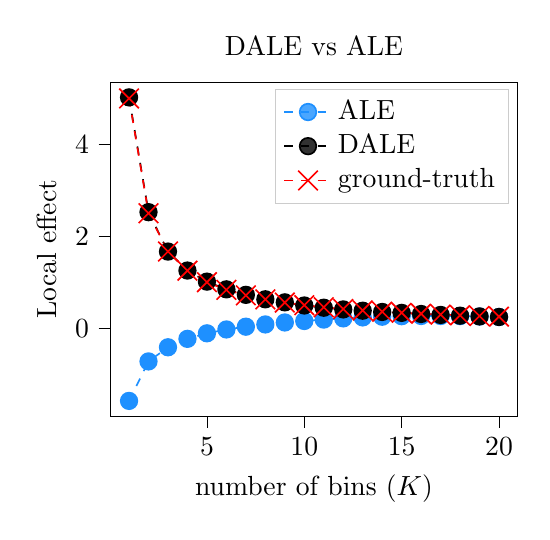
\begin{tikzpicture}

\definecolor{darkgray176}{RGB}{176,176,176}
\definecolor{dodgerblue}{RGB}{30,144,255}
\definecolor{lightgray204}{RGB}{204,204,204}

\begin{axis}[
legend cell align={left},
legend style={fill opacity=0.8, draw opacity=1, text opacity=1, draw=lightgray204},
tick align=outside,
tick pos=left,
title={DALE vs ALE},
x grid style={darkgray176},
xlabel={number of bins \(\displaystyle (K)\)},
xmin=0.0499999999999999, xmax=20.95,
xtick style={color=black},
y grid style={darkgray176},
ylabel={Local effect},
ymin=-1.91455718867646, ymax=5.35298172476343,
ytick style={color=black}
]
\addplot [semithick, dodgerblue, dashed, mark=*, mark size=3, mark options={solid}]
table {%
1 -1.58421451079283
2 -0.724791391897207
3 -0.416931226166923
4 -0.233523181012335
5 -0.113002110067188
6 -0.0293908088400257
7 0.0312305603326059
8 0.0797401389995273
9 0.12275670716894
10 0.155053447821085
11 0.186088568383995
12 0.211864987771331
13 0.233108878251814
14 0.247869171569635
15 0.259566596177554
16 0.264108921400541
17 0.263569771086526
18 0.260892620884744
19 0.252751953555994
20 0.242460730712491
};
\addlegendentry{ALE}
\addplot [semithick, black, dashed, mark=*, mark size=3, mark options={solid}]
table {%
1 5.0226390468798
2 2.52393513932938
3 1.66605371806444
4 1.25321810135996
5 1.01182618748851
6 0.844347970008633
7 0.723984251300441
8 0.627612080163916
9 0.560862770386464
10 0.492398374084428
11 0.444051023514039
12 0.4070407257714
13 0.379038857924861
14 0.351678147881759
15 0.331857705495926
16 0.307844113455479
17 0.286910008925387
18 0.270908782811331
19 0.254748495290572
20 0.24246073071272
};
\addlegendentry{DALE}
\addplot [semithick, red, dashed, mark=x, mark size=5, mark options={solid}]
table {%
1 5
2 2.5
3 1.66666666666667
4 1.25
5 1
6 0.833333333333333
7 0.714285714285714
8 0.625
9 0.555555555555556
10 0.5
11 0.454545454545455
12 0.416666666666667
13 0.384615384615385
14 0.357142857142857
15 0.333333333333333
16 0.3125
17 0.294117647058824
18 0.277777777777778
19 0.263157894736842
20 0.25
};
\addlegendentry{ground-truth}
\end{axis}

\end{tikzpicture}
}
  \caption[Example comparison]{(Left) The black-box function \(f\) of
    Section~\ref{sec:4-3-robustness}. (Right) Estimation of the bin
    effect of the first bin for DALE and ALE, for varying number of
    bins \(K\).}
  \label{fig:example-different-bins}
\end{figure}


\subsection{Bias and variance}
\label{sec:4-4-std}
Let a finite dataset of samples \(\mathcal{S}\), drawn independently
and identically distributed (i.i.d) from the data generating
distribution of \(\mathcal{X}\). DALE computes the accumulated local
effect (Eq.~\eqref{eq:ALE}), using the approximation in
(Eq.~\eqref{eq:DALE}). The expected value of the approximation across
different datasets is

\begin{equation}
  \mathbb{E}_{\mathcal{S}}[\dale(x)] =
  \Delta x\sum_{k=1}^{k_x}\mathbb{E}_{\mathcal{S}}[\frac{1}{|\mathcal{S}_k|}\sum_{i:\xb^i \in
      \mathcal{S}_k} f_s(\xb^i)]
  \label{eq:bias_dale}
\end{equation}

\noindent
Notice also that for the values of \(x\) at the end of bin \(k_x\),
Eq.~\eqref{eq:ALE} can be rewritten as (after omitting the constant
\(c\))
\begin{equation}
  f_{\mathtt{ALE}}(x) = \sum_{k = 1}^{k_x}\int_{x_{k-1}}^{x_k}
    \mathbb{E}_{\Xcb|\mathcal{X}_s=z}[f_s(\xb)] \partial z
    \label{eq:bias_ale_1}
\end{equation}
where \(x_0=x_{s, min}\) and \(x_i\), \(i=1, \dotsc, k_x\) are the bin limits.

\noindent
If we assume that each bin is sufficiently small such that \(f_s(\xb)\) does
not depend on \(x_s\) (i.e., \(f(x)\) is linear wrt \(x_s\)) within the bin, then
Eq. \eqref{eq:bias_ale_1} becomes
\begin{equation}
  f_{\mathtt{ALE}}(x) = \sum_{k = 1}^{k_x}\mathbb{E}_{\Xcb|\mathcal{X}_s \in
    \mathcal{S}_k}[f_s(\xb)]\int_{x_{k-1}}^{x_k} \partial z
  = \Delta x\sum_{k=1}^{k_x}\mathbb{E}_{\mathcal{X} \in \mathcal{S}_k}[f_s(\xb)]
    \label{eq:bias_ale_2}
\end{equation}

\noindent
From Eqs. \eqref{eq:bias_dale} and \eqref{eq:bias_ale_2} we have
\begin{multline}
    \mathbb{E}_{\mathcal{S}}[\dale]  - f_{\mathtt{ALE}}(x) =
    \Delta x\sum_{k=1}^{k_x}\mathbb{E}_{\mathcal{S}}[\frac{1}{|\mathcal{S}_k|}\sum_{k:\xb^k \in
        \mathcal{S}_k} f_s(\xb^k)] - \\
    \Delta x\sum_{k=1}^{k_x}\mathbb{E}_{\mathcal{X}\in \mathcal{S}_k}[f_s(\xb)] =
  \Delta x\sum_{k=1}^{k_x}\left(\mathbb{E}_{\mathcal{S}}[\hat{\mu}_k^s] - \mu_k^s\right) = 0
\end{multline}
since the expected value of the sample mean is an unbiased estimator
of \(\mu_k^s\). As a result, under the condition of linearity wrt
\(x_s\) within the bin, DALE is an unbiased estimator of the feature
effect. If this assumption is violated (e.g., large bin size or highly
nonlinear function), then this approach may introduce bias. The
variance of the estimator is given\footnote{We show that in the
  supporting material.} by
\( \mathrm{Var}[\hat{\mu}_k^s] =
\dfrac{(\sigma_k^s)^2}{|\mathcal{S}_k|} \), where \((\sigma_k^s)^2\)
is the variance of \(f_s\) within the bin. Furthermore, since the
samples \(\xb^i\) are independent, \(\hat{\mu}_k^s\) for
\(k=1,\dotsc,k_x\) are also independent. The variance of the
estimation can then be approximated as
%
\begin{equation}
  \mathrm{Var}[\dale(x)] = (\Delta x)^2\sum_k^{k_x} \mathrm{Var} [\hat{\mu}_k^s]
  = (\Delta x)^2 \sum_k^{k_x}  \dfrac{(\sigma_k^s)^2}{|\mathcal{S}_k|} \approx
  (\Delta x)^2 \sum_k^{k_x}  \dfrac{(\hat{\sigma}_k^s)^2}{|\mathcal{S}_k|}
  \label{eq:DALE-var}
\end{equation}
%
where \((\hat{\sigma}_k^s)^2\) is the sample variance within bin
\(k\). Equation~\eqref{eq:DALE-var} allows the calculation of the
standard error for the DALE approximation.


% \subsection{Limitations of DALE}
% \label{sec:3-5-limitations}
% \input{./chapters/3-5-limitations.tex}

\section{Experiments}

This section presents the experimental evaluation of DALE using two
synthetic and one real dataset. The experiments aim to compare DALE
(\(\dale\)) with ALE approximation
(\(\hat{f}_{\mathtt{ALE}}\)) from the perspectives of both efficiency
and accuracy.

\paragraph{Metrics.} For evaluating the efficiency of the
approximations we measure the execution times (in seconds). For
evaluating the accuracy we use: (a) qualitative comparison of the
feature effect plots and (b) the Normalized Mean Squared Error which
is defined as
\(\text{NMSE}_{\mathtt{<approx>}} = \frac{\E[(\ale -
  f_{\mathtt{<approx>}})^2]}{\text{Var}[\ale]}\).

\paragraph{Synthetic Datasets.} The first synthetic dataset (Case 1) is designed
to compare the approximations in terms of efficiency. For this reason,
we generate design matrices \(\mathbf{X}\) of varying dimensionality
\(D\) and number of instances \(N\). The second synthetic dataset
(Case 2) is designed to compare the approximations in terms of
accuracy. We define a data generating distribution \(\mathcal{X}\) and
a black box function \(f\) with known forms for being able to directly
compute the ground-truth ALE from Eq.~\eqref{eq:ALE}. Both
\(\mathcal{X}\) and \(f\) are designed to amplify the effect of OOD
sampling.

\paragraph{Real Dataset} We choose the Bike-Sharing dataset for two
reasons. Firstly, it is the dataset utilized in the original ALE
paper, so it is a proper choice for unbiased comparisons. Secondly, we
wanted a dataset with enough training points to approximate the
feature effect accurately, since the ground-truth is not
available. Therefore, we want to check that \(\dale\) and
\(\hat{f}_{\mathtt{ALE}}\) provide similar effects using dense
bins. We also evaluate the accuracy of both methods behave when using
larger bins.

\subsection{Synthetic Datasets}
\label{sec:5-1-artificial-experiments}
\subsubsection{Case 1 - Efficiency comparison}
\label{sec:case-1}

In this example, we evaluate the efficiency of the two approximations,
\(\dale\) and \(\hat{f}_{\mathtt{ALE}}\), through the
execution times. We want to compare how both approximations perform in
terms of the dimensionality of the problem (\(D\)), the dataset size
(\(N\)) and the size of the model \(L\). In each experiment we
generate a design-matrix \( \mathbf{X} \), by drawing \( N \cdot D \)
samples from a standard normal distribution. The black-box function
\(f \) is a fully-connected neural network with \(L\) hidden layers of
\( 1024 \) units each. All experiments are done using \(K=100\). We
want to clarify that the value of \(K\) plays almost no role in the
execution times.

In Figure~\Ref{fig:case-1-plots-1}, we directly compare
\(\dale\) and \(\hat{f}_{\mathtt{ALE}}\) in two different
setups: in Figure~\Ref{fig:case-1-plots-1}(Left), we use a light setup
of \(N=10^3\) examples and a model of \(L=2\) layers, whereas in
Figure~\Ref{fig:case-1-plots-1}(Right), a heavier setup with
\(N=10^5\) and \(L=6\). We observe that in both cases, DALE executes
in near-constant time independently of \(D\), while ALE scales
linearly with wrt \(D\), confirming our claims of
Section~\ref{sec:4-2-computational}. The difference in the execution
time reaches significant levels from a relatively small
dimensionality. In the heavy setup, ALE needs almost a minute for
\(D=20\), three minutes for \(D=50\), and 15 minutes for \(D=100\). In
all these cases, DALE executes in a few seconds. Another critical
remark is that DALE's execution time is almost identical to the
computation of the Jacobian \( \Jac \), which is benefited by
automatic differentiation. Hence, we confirm that the overhead of
performing steps 3-5 of Algorithm~\ref{alg:dale} is a small fraction
of the total execution time. Another consequence of this remark is
that we can test many different bin sizes with near-zero computational
cost.

In Figure~\Ref{fig:case-1-plots-2}, we rigorously quantify to what
extent the dataset size \(N\) and the model size \(L\) affect both
methods. In Figures~\Ref{fig:case-1-plots-2}(a) and
~\Ref{fig:case-1-plots-2}(c), we confirm that both \(N\) and \(L\)
have crucial impact in ALE's execution times. Therefore, for a big
dataset and a heavy model \(f\), ALE's execution time quickly reaches
prohibitive levels. In contrast, in
Figures~\Ref{fig:case-1-plots-2}(b) and
Figures~\Ref{fig:case-1-plots-2}(d), DALE is negligibly affected by
these parameters. In the figures, we restrict the experiment to cases
up to 100-dimensional input for illustration purposes. The same trend
continues for an arbitrary number of dimensions. DALE can scale
efficiently to any dimensionality as long as we have enough resources
to store the dataset, evaluate the prediction model \(f\) and apply
the gradients \(\nabla_{\xb}f\).

\begin{figure}[h]
  \centering
  \resizebox{.4\columnwidth}{!}{% This file was created with tikzplotlib v0.10.1.
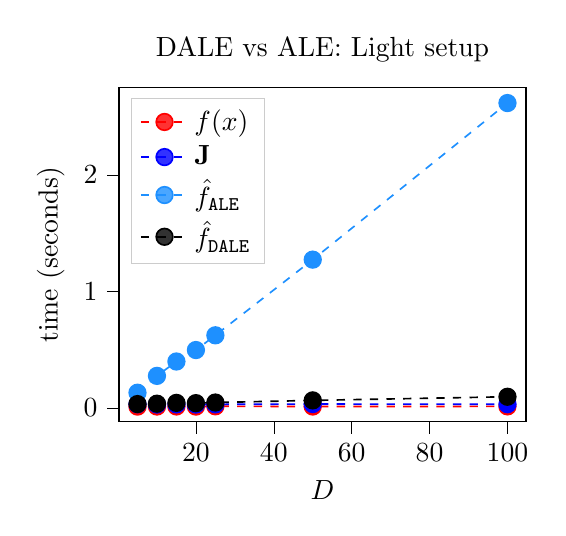
\begin{tikzpicture}

\definecolor{darkgray176}{RGB}{176,176,176}
\definecolor{dodgerblue}{RGB}{30,144,255}
\definecolor{lightgray204}{RGB}{204,204,204}

\begin{axis}[
legend cell align={left},
legend style={
  fill opacity=0.8,
  draw opacity=1,
  text opacity=1,
  at={(0.03,0.97)},
  anchor=north west,
  draw=lightgray204
},
tick align=outside,
tick pos=left,
title={DALE vs ALE: Light setup},
x grid style={darkgray176},
xlabel={\(\displaystyle D\)},
xmin=0.25, xmax=104.75,
xtick style={color=black},
y grid style={darkgray176},
ylabel={time (seconds)},
ymin=-0.118335867500491, ymax=2.74596303149951,
ytick style={color=black}
]
\addplot [semithick, red, dashed, mark=*, mark size=3, mark options={solid}]
table {%
5 0.0118595361709595
10 0.0122641324996948
15 0.0128312110900879
20 0.0119729042053223
25 0.0144194364547729
50 0.0124425888061523
100 0.0135363340377808
};
\addlegendentry{$f(x)$}
\addplot [semithick, blue, dashed, mark=*, mark size=3, mark options={solid}]
table {%
5 0.0321429967880249
10 0.0295344591140747
15 0.0305428504943848
20 0.0298470258712769
25 0.0309284925460815
50 0.0336670875549316
100 0.032146692276001
};
\addlegendentry{$\mathbf{J}$}
\addplot [semithick, dodgerblue, dashed, mark=*, mark size=3, mark options={solid}]
table {%
5 0.130752086639404
10 0.275371313095093
15 0.398597836494446
20 0.496960043907166
25 0.623412370681763
50 1.27240407466888
100 2.61576771736145
};
\addlegendentry{$\hat{f}_{\mathtt{ALE}}$}
\addplot [semithick, black, dashed, mark=*, mark size=3, mark options={solid}]
table {%
5 0.0335890054702759
10 0.0366946458816528
15 0.0436010360717773
20 0.0414165258407593
25 0.0466822385787964
50 0.0650126934051514
100 0.0961912870407104
};
\addlegendentry{$\hat{f}_{\mathtt{DALE}}$}
\end{axis}

\end{tikzpicture}
}
  \resizebox{.43\columnwidth}{!}{% This file was created with tikzplotlib v0.10.1.
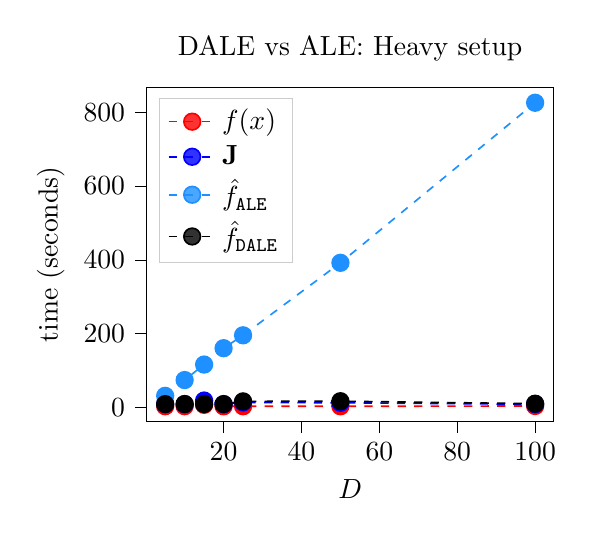
\begin{tikzpicture}

\definecolor{darkgray176}{RGB}{176,176,176}
\definecolor{dodgerblue}{RGB}{30,144,255}
\definecolor{lightgray204}{RGB}{204,204,204}

\begin{axis}[
legend cell align={left},
legend style={
  fill opacity=0.8,
  draw opacity=1,
  text opacity=1,
  at={(0.03,0.97)},
  anchor=north west,
  draw=lightgray204
},
tick align=outside,
tick pos=left,
title={DALE vs ALE: Heavy setup},
x grid style={darkgray176},
xlabel={\(\displaystyle D\)},
xmin=0.25, xmax=104.75,
xtick style={color=black},
y grid style={darkgray176},
ylabel={time (seconds)},
ymin=-38.1810145603003, ymax=867.056094992299,
ytick style={color=black}
]
\addplot [semithick, red, dashed, mark=*, mark size=3, mark options={solid}]
table {%
5 3.13364505767822
10 3.24496150016785
15 6.86045789718628
20 2.96612668037415
25 3.05197858810425
50 3.02510833740234
100 3.71672296524048
};
\addlegendentry{$f(x)$}
\addplot [semithick, blue, dashed, mark=*, mark size=3, mark options={solid}]
table {%
5 8.88222980499268
10 8.82908821105957
15 18.4925575256348
20 8.51719951629639
25 13.5228071212769
50 12.4858655929565
100 8.59451198577881
};
\addlegendentry{$\mathbf{J}$}
\addplot [semithick, dodgerblue, dashed, mark=*, mark size=3, mark options={solid}]
table {%
5 31.310697555542
10 74.1438674926758
15 116.133689880371
20 160.465118408203
25 195.409912109375
50 391.950622558594
100 825.908935546875
};
\addlegendentry{$\hat{f}_{\mathtt{ALE}}$}
\addplot [semithick, black, dashed, mark=*, mark size=3, mark options={solid}]
table {%
5 8.83595371246338
10 9.03882694244385
15 9.21370220184326
20 8.9499044418335
25 16.3313121795654
50 16.7110271453857
100 10.0340776443481
};
\addlegendentry{$\hat{f}_{\mathtt{DALE}}$}
\end{axis}

\end{tikzpicture}
}
  \caption[Case-1-fig-1]{Case 1. Comparison of the execution time of DALE
    and ALE in two setups: (Left) Light setup; \(N=10^3, L=2\).
    (Right) Light setup; \(N=10^5, L=6\)}
  \label{fig:case-1-plots-1}
\end{figure}

\begin{figure}[h]
  \centering
  \resizebox{.23\columnwidth}{!}{% This file was created with tikzplotlib v0.10.1.
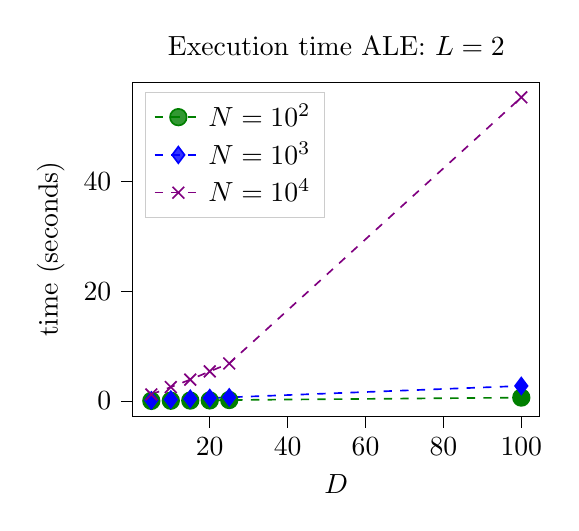
\begin{tikzpicture}

\definecolor{darkgray176}{RGB}{176,176,176}
\definecolor{green01270}{RGB}{0,127,0}
\definecolor{lightgray204}{RGB}{204,204,204}
\definecolor{purple}{RGB}{128,0,128}

\begin{axis}[
legend cell align={left},
legend style={
  fill opacity=0.8,
  draw opacity=1,
  text opacity=1,
  at={(0.03,0.97)},
  anchor=north west,
  draw=lightgray204
},
tick align=outside,
tick pos=left,
title={Execution time ALE: \(\displaystyle L=2\)},
x grid style={darkgray176},
xlabel={\(\displaystyle D\)},
xmin=0.25, xmax=104.75,
xtick style={color=black},
y grid style={darkgray176},
ylabel={time (seconds)},
ymin=-2.73388298709979, ymax=57.999057591099,
ytick style={color=black}
]
\addplot [semithick, green01270, dashed, mark=*, mark size=3, mark options={solid}]
table {%
5 0.026705265045166
10 0.0574851036071777
15 0.0858516693115234
20 0.112214326858521
25 0.184911131858826
100 0.628105640411377
};
\addlegendentry{$N=10^2$}
\addplot [semithick, blue, dashed, mark=diamond*, mark size=3, mark options={solid}]
table {%
5 0.127141833305359
10 0.271587371826172
15 0.413034200668335
20 0.54520583152771
25 0.675822854042053
100 2.74792742729187
};
\addlegendentry{$N=10^3$}
\addplot [semithick, purple, dashed, mark=x, mark size=3, mark options={solid}]
table {%
5 1.20529174804688
10 2.53928112983704
15 3.89853239059448
20 5.39064311981201
25 6.83541965484619
100 55.238468170166
};
\addlegendentry{$N=10^4$}
\end{axis}

\end{tikzpicture}
}
  \resizebox{.23\columnwidth}{!}{% This file was created with tikzplotlib v0.10.1.
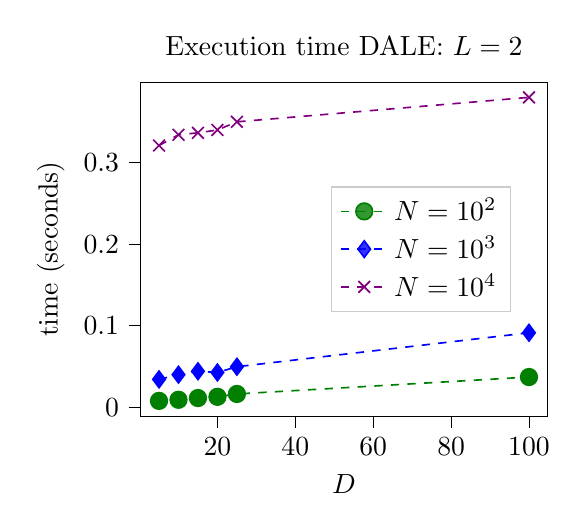
\begin{tikzpicture}

\definecolor{darkgray176}{RGB}{176,176,176}
\definecolor{green01270}{RGB}{0,127,0}
\definecolor{lightgray204}{RGB}{204,204,204}
\definecolor{purple}{RGB}{128,0,128}

\begin{axis}[
legend cell align={left},
legend style={
  fill opacity=0.8,
  draw opacity=1,
  text opacity=1,
  at={(0.91,0.5)},
  anchor=east,
  draw=lightgray204
},
tick align=outside,
tick pos=left,
title={Execution time DALE: \(\displaystyle L=2\)},
x grid style={darkgray176},
xlabel={\(\displaystyle D\)},
xmin=0.25, xmax=104.75,
xtick style={color=black},
y grid style={darkgray176},
ylabel={time (seconds)},
ymin=-0.0109329749522149, ymax=0.398615855950105,
ytick style={color=black}
]
\addplot [semithick, green01270, dashed, mark=*, mark size=3, mark options={solid}]
table {%
5 0.0076829195022583
10 0.00905656814575195
15 0.0112016201019287
20 0.0126841068267822
25 0.0161861181259155
100 0.0369504690170288
};
\addlegendentry{$N=10^2$}
\addplot [semithick, blue, dashed, mark=diamond*, mark size=3, mark options={solid}]
table {%
5 0.0340769290924072
10 0.0398837327957153
15 0.0440537929534912
20 0.0425540208816528
25 0.0495928525924683
100 0.0912438631057739
};
\addlegendentry{$N=10^3$}
\addplot [semithick, purple, dashed, mark=x, mark size=3, mark options={solid}]
table {%
5 0.320958256721497
10 0.334092974662781
15 0.33648693561554
20 0.340000033378601
25 0.350000023841858
100 0.379999995231628
};
\addlegendentry{$N=10^4$}
\end{axis}

\end{tikzpicture}
}
  \resizebox{.23\columnwidth}{!}{% This file was created with tikzplotlib v0.10.1.
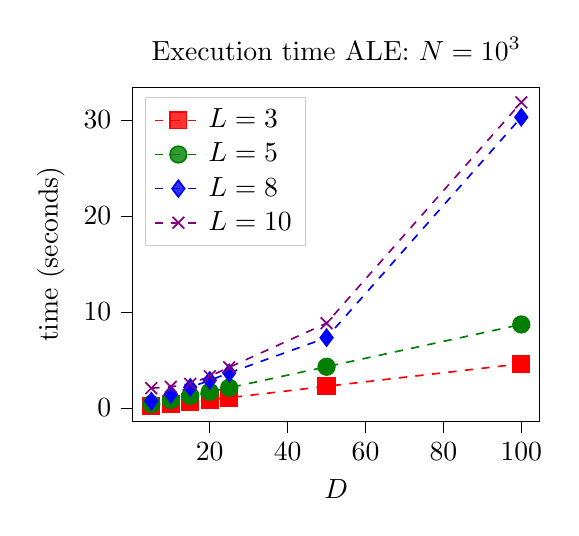
\begin{tikzpicture}

\definecolor{darkgray176}{RGB}{176,176,176}
\definecolor{green01270}{RGB}{0,127,0}
\definecolor{lightgray204}{RGB}{204,204,204}
\definecolor{purple}{RGB}{128,0,128}

\begin{axis}[
legend cell align={left},
legend style={
  fill opacity=0.8,
  draw opacity=1,
  text opacity=1,
  at={(0.03,0.97)},
  anchor=north west,
  draw=lightgray204
},
tick align=outside,
tick pos=left,
title={Execution time ALE: \(\displaystyle N=10^3\)},
x grid style={darkgray176},
xlabel={\(\displaystyle D\)},
xmin=0.25, xmax=104.75,
xtick style={color=black},
y grid style={darkgray176},
ylabel={time (seconds)},
ymin=-1.36616255235276, ymax=33.4035613893502,
ytick style={color=black}
]
\addplot [semithick, red, dashed, mark=square*, mark size=3, mark options={solid}]
table {%
5 0.214279413223267
10 0.445428252220154
15 0.637093186378479
20 0.876859426498413
25 1.06718361377716
50 2.25691056251526
100 4.60215711593628
};
\addlegendentry{$L=3$}
\addplot [semithick, green01270, dashed, mark=*, mark size=3, mark options={solid}]
table {%
5 0.408349752426147
10 0.824460029602051
15 1.26256990432739
20 1.68054091930389
25 2.10548663139343
50 4.29162120819092
100 8.69534683227539
};
\addlegendentry{$L=5$}
\addplot [semithick, blue, dashed, mark=diamond*, mark size=3, mark options={solid}]
table {%
5 0.71037769317627
10 1.42690515518188
15 2.14693737030029
20 2.87370538711548
25 3.65433740615845
50 7.31730794906616
100 30.2758731842041
};
\addlegendentry{$L=8$}
\addplot [semithick, purple, dashed, mark=x, mark size=3, mark options={solid}]
table {%
5 2.06213808059692
10 2.20000004768372
15 2.5
20 3.30623149871826
25 4.2340202331543
50 8.82898712158203
100 31.8231201171875
};
\addlegendentry{$L=10$}
\end{axis}

\end{tikzpicture}
}
  \resizebox{.23\columnwidth}{!}{% This file was created with tikzplotlib v0.10.1.
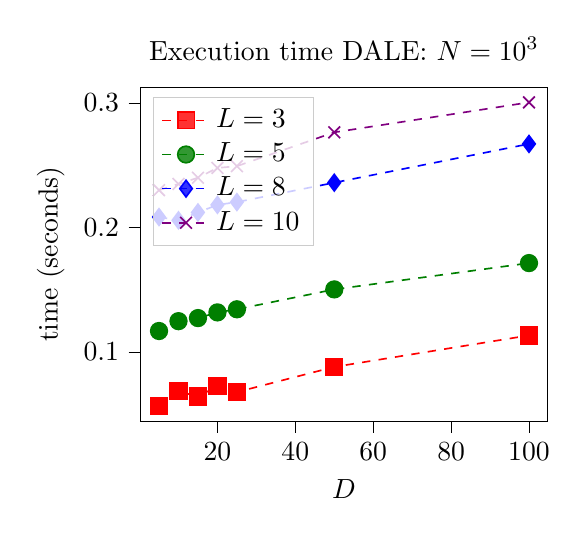
\begin{tikzpicture}

\definecolor{darkgray176}{RGB}{176,176,176}
\definecolor{green01270}{RGB}{0,127,0}
\definecolor{lightgray204}{RGB}{204,204,204}
\definecolor{purple}{RGB}{128,0,128}

\begin{axis}[
legend cell align={left},
legend style={
  fill opacity=0.8,
  draw opacity=1,
  text opacity=1,
  at={(0.03,0.97)},
  anchor=north west,
  draw=lightgray204
},
tick align=outside,
tick pos=left,
title={Execution time DALE: \(\displaystyle N=10^3\)},
x grid style={darkgray176},
xlabel={\(\displaystyle D\)},
xmin=0.25, xmax=104.75,
xtick style={color=black},
y grid style={darkgray176},
ylabel={time (seconds)},
ymin=0.0445653210494129, ymax=0.312711131950527,
ytick style={color=black}
]
\addplot [semithick, red, dashed, mark=square*, mark size=3, mark options={solid}]
table {%
5 0.0567537546157837
10 0.0685902833938599
15 0.0642098188400269
20 0.0725626945495605
25 0.0678497552871704
50 0.088062047958374
100 0.113367915153503
};
\addlegendentry{$L=3$}
\addplot [semithick, green01270, dashed, mark=*, mark size=3, mark options={solid}]
table {%
5 0.116896510124207
10 0.124809384346008
15 0.127277135848999
20 0.131840586662292
25 0.134345889091492
50 0.150314569473267
100 0.171453237533569
};
\addlegendentry{$L=5$}
\addplot [semithick, blue, dashed, mark=diamond*, mark size=3, mark options={solid}]
table {%
5 0.208409428596497
10 0.205777525901794
15 0.212119460105896
20 0.218204021453857
25 0.220425486564636
50 0.236039161682129
100 0.267152309417725
};
\addlegendentry{$L=8$}
\addplot [semithick, purple, dashed, mark=x, mark size=3, mark options={solid}]
table {%
5 0.230000019073486
10 0.235000014305115
15 0.240000009536743
20 0.247859835624695
25 0.249285697937012
50 0.276461362838745
100 0.300522685050964
};
\addlegendentry{$L=10$}
\end{axis}

\end{tikzpicture}
}
  \caption[Case-1-fig-2]{Case 1. Measurements of the execution time wrt dimensionality \(D\):
    (a) \(\hat{f}_{\mathtt{ALE}}\) for \(L = 2\), and many dataset sizes \(N\)
    (b) \(\hat{f}_{\mathtt{ALE}}\) for \(N = 10^3\), and many model sizes \(L\)
    (c) \(\dale\) for \(L = 2\), and many dataset sizes \(N\)
    (d) \(\dale\) for \(N = 10^3\), and many model sizes \(L\)
  }
  \label{fig:case-1-plots-2}
\end{figure}


\subsubsection{Case 2 - Accuracy Comparison}
\label{sec:example2}

In this example, we evaluate the accuracy of the two approximations,
\(\dale\) and \(\hat{f}_{\mathtt{ALE}}\), in a synthetic
dataset where the ground truth ALE is accessible. As discussed in
Section~\ref{sec:4-3-robustness}, ALE approximation is vulnerable to
OOD sampling when the bins are wide, or equivalently, the number of
bins \(K\) is small. We want to compare how both approximations behave
in a case where the local effect is noisy.
%
We design an experiment where we know the black-box function and the
data generating distribution. The black-box function
\(f:\R^3 \rightarrow \R\) is split in three parts to amplify the
effect of OOD sampling. It includes a mild term
\( f_0(x) = x_1x_2 + x_1x_3 \) in the region
\( 0 \leq |x_1 - x_2| < \tau \) and then a quadratic term
\(g(x) = \alpha ((x_1 - x_2)^2 - \tau^2)\) is added(subtracted)
over(under) the region, i.e.:

\begin{equation} \label{eq:example-2-mapping}
  f(\mathbf{x}) =
  \begin{cases}
    f_0(x) & , 0 \leq |x_1 - x_2|  < \tau \\
    f_0(x) - g(x) & , \tau \leq |x_1 - x_2|  \\
    f_0(x) + g(x) & , \tau \leq - |x_1 - x_2|  \\
  \end{cases}
\end{equation}

\noindent
%
The data points \(X^i = (x_1^i, x_2^i, x_3^i)\) are generated as
follows; \(x_1^i \) are clustered around the points
\(\{1.5, 3, 5, 7, 8.5\}\),
\(x_2^i \sim \mathcal{N}(\mu=x_1, \sigma_2=0.1) \) and
\(x_3^i \sim \mathcal{N}(\mu=0, \sigma_3^2=10) \). In
Figure~\ref{fig:example-2-samples}(a), we illustrate \(f(\xb)\) for
\(x_3=0\), as well as the generated data points. In this example, the
local effect of \(x_1\) is
\(\frac{\partial f}{\partial x_1} = x_2 + x_3\). Due to the noisy
nature of \(x_3\), both ALE and DALE need a large number of sample for
robust estimation. Therefore, we need to lower the number of bins
\(K\). As will be shown below, both ALE and DALE fail to approximate
the feature effect for high \(K\). On the other hand, when using a
lower \(K\), ALE approximation fails due to OOD sampling, while DALE
manages to accurately approximate the feature effect.

In Figure~\ref{fig:example-2-samples}(b) and
Figure~\ref{fig:example-2-samples}(c), we observe the estimated
effects for \(K=50\) and \(K=5\). In
Figure~\ref{fig:example-2-samples}(b), \((K=50)\) the approximations
converge to the same estimated effect which is inaccurate due to many
noisy artifacts. In Figure~\ref{fig:example-2-samples}(c), \((K=5)\)
we observe that for small \(K\), DALE approximates the ground-truth
effect well, whereas ALE fails due to OOD
sampling. Table~\ref{tab:case-2-accuracy} provides the NMSE of both
approximation for varying number of bins \(K\). We observe that DALE
consistently provides accurate estimations (NMSE \(\leq 0.1\)) for all
small \(K\) values.

The experiments helps us confirm that when \(K \) increases, both
approximations are based on a limited number of samples, and are
vulnerable to noise. When \(K\) decreases, DALE lowers the resolution
but provides more robust estimations. In contrast, ALE is vulnerable
to OOD sampling.

\begin{table}
  \centering
  \caption{Case 2. Evaluation of the NMSE between the approximations and the ground truth. Blue color indicates the values that are below \(0.1\).}
  \label{tab:case-2-accuracy}
  \begin{tabular}{c|c|c|c|c|c|c|c|c|c}
    \multicolumn{10}{c}{Accuracy on the Synthetic Dataset (Case 2)} \\
    \hline \hline
    & & \multicolumn{8}{|c}{Number of bins} \\
    \hline
    & & 1 & 2 & 3 & 4 & 5 & 10 & 20 & 40 \\
    \hline
    \hline
    \multirow{2}{*}{\(\mathtt{NMSE}\)} & \(\dale\) & \textcolor{blue}{0.10} & \textcolor{blue}{0.03} & \textcolor{blue}{0.09} & \textcolor{blue}{0.02} & \textcolor{blue}{0.02} & 0.82 & 0.24 & 0.38\\
    & \(\alep\) & 100.42 & 22.09 & 4.97 & 2.81 & 0.78 & 1.49 & 0.34 & 0.39 \\
    \hline
  \end{tabular}
\end{table}


\begin{figure}[h]
  \begin{center}
    \resizebox{.33\columnwidth}{!}{% This file was created with tikzplotlib v0.10.1.
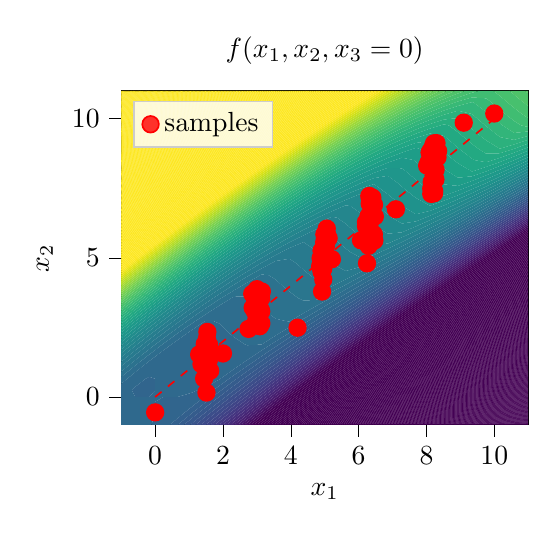
\begin{tikzpicture}

\definecolor{darkcyan30153138}{RGB}{30,153,138}
\definecolor{darkcyan30157136}{RGB}{30,157,136}
\definecolor{darkcyan31146140}{RGB}{31,146,140}
\definecolor{darkcyan31150139}{RGB}{31,150,139}
\definecolor{darkcyan31162134}{RGB}{31,162,134}
\definecolor{darkcyan33141140}{RGB}{33,141,140}
\definecolor{darkcyan34137141}{RGB}{34,137,141}
\definecolor{darkcyan36134141}{RGB}{36,134,141}
\definecolor{darkcyan37130142}{RGB}{37,130,142}
\definecolor{darkcyan39125142}{RGB}{39,125,142}
\definecolor{darkgray176}{RGB}{176,176,176}
\definecolor{darkslateblue47105141}{RGB}{47,105,141}
\definecolor{darkslateblue49101141}{RGB}{49,101,141}
\definecolor{darkslateblue5196141}{RGB}{51,96,141}
\definecolor{darkslateblue5392140}{RGB}{53,92,140}
\definecolor{darkslateblue5588140}{RGB}{55,88,140}
\definecolor{darkslateblue5784139}{RGB}{57,84,139}
\definecolor{darkslateblue6078138}{RGB}{60,78,138}
\definecolor{darkslateblue6174137}{RGB}{61,74,137}
\definecolor{darkslateblue6369135}{RGB}{63,69,135}
\definecolor{darkslateblue6565134}{RGB}{65,65,134}
\definecolor{darkslateblue6759131}{RGB}{67,59,131}
\definecolor{darkslateblue6954129}{RGB}{69,54,129}
\definecolor{darkslateblue7049126}{RGB}{70,49,126}
\definecolor{darkslateblue7138118}{RGB}{71,38,118}
\definecolor{darkslateblue7144123}{RGB}{71,44,123}
\definecolor{gold21822624}{RGB}{218,226,24}
\definecolor{gold22822724}{RGB}{228,227,24}
\definecolor{gold23822927}{RGB}{238,229,27}
\definecolor{gold24823033}{RGB}{248,230,33}
\definecolor{gold25323136}{RGB}{253,231,36}
\definecolor{greenyellow19422334}{RGB}{194,223,34}
\definecolor{greenyellow20522429}{RGB}{205,224,29}
\definecolor{indigo68184}{RGB}{68,1,84}
\definecolor{indigo68387}{RGB}{68,3,87}
\definecolor{indigo70992}{RGB}{70,9,92}
\definecolor{indigo711598}{RGB}{71,15,98}
\definecolor{indigo7121103}{RGB}{71,21,103}
\definecolor{indigo7228110}{RGB}{72,28,110}
\definecolor{indigo7233114}{RGB}{72,33,114}
\definecolor{lightgray204}{RGB}{204,204,204}
\definecolor{mediumseagreen10720589}{RGB}{107,205,89}
\definecolor{mediumseagreen33166133}{RGB}{33,166,133}
\definecolor{mediumseagreen35169130}{RGB}{35,169,130}
\definecolor{mediumseagreen40174127}{RGB}{40,174,127}
\definecolor{mediumseagreen44177125}{RGB}{44,177,125}
\definecolor{mediumseagreen50181122}{RGB}{50,181,122}
\definecolor{mediumseagreen56185118}{RGB}{56,185,118}
\definecolor{mediumseagreen64189114}{RGB}{64,189,114}
\definecolor{mediumseagreen71192110}{RGB}{71,192,110}
\definecolor{mediumseagreen79195105}{RGB}{79,195,105}
\definecolor{mediumseagreen87198101}{RGB}{87,198,101}
\definecolor{mediumseagreen9820295}{RGB}{98,202,95}
\definecolor{steelblue46109142}{RGB}{46,109,142}
\definecolor{teal40122142}{RGB}{40,122,142}
\definecolor{teal42118142}{RGB}{42,118,142}
\definecolor{teal44114142}{RGB}{44,114,142}
\definecolor{yellowgreen11620884}{RGB}{116,208,84}
\definecolor{yellowgreen12621078}{RGB}{126,210,78}
\definecolor{yellowgreen13921370}{RGB}{139,213,70}
\definecolor{yellowgreen14921563}{RGB}{149,215,63}
\definecolor{yellowgreen15921756}{RGB}{159,217,56}
\definecolor{yellowgreen17322048}{RGB}{173,220,48}
\definecolor{yellowgreen18322141}{RGB}{183,221,41}

\begin{axis}[
legend cell align={left},
legend style={
  fill opacity=0.8,
  draw opacity=1,
  text opacity=1,
  at={(0.03,0.97)},
  anchor=north west,
  draw=lightgray204
},
tick align=outside,
tick pos=left,
title={\(\displaystyle f(x_1, x_2, x_3=0)\)},
x grid style={darkgray176},
xlabel={\(\displaystyle x_1\)},
xmin=-1, xmax=11,
xtick style={color=black},
y grid style={darkgray176},
ylabel={\(\displaystyle x_2\)},
ymin=-1, ymax=11,
ytick style={color=black}
]
\addplot [draw=none, fill=indigo68184, forget plot]
table{%
x  y
11 -1
11 -0.977740356373605
10.9764002491177 -1
11 -1
};
\addplot [draw=none, fill=indigo68184, forget plot]
table{%
x  y
11 -0.977740356373605
11 -0.949347953788917
10.9462985260536 -1
10.9764002491177 -1
11 -0.977740356373605
};
\addplot [draw=none, fill=indigo68184, forget plot]
table{%
x  y
11 -0.949347953788917
11 -0.92095555120423
10.9161968029894 -1
10.9462985260536 -1
11 -0.949347953788917
};
\addplot [draw=none, fill=indigo68184, forget plot]
table{%
x  y
11 -0.92095555120423
11 -0.892563148619542
10.8860950799253 -1
10.9161968029894 -1
11 -0.92095555120423
};
\addplot [draw=none, fill=indigo68184, forget plot]
table{%
x  y
11 -0.892563148619542
11 -0.864170746034854
10.8559933568611 -1
10.8860950799253 -1
11 -0.892563148619542
};
\addplot [draw=none, fill=indigo68184, forget plot]
table{%
x  y
11 -0.864170746034854
11 -0.835778343450167
10.825891633797 -1
10.8559933568611 -1
11 -0.864170746034854
};
\addplot [draw=none, fill=indigo68184, forget plot]
table{%
x  y
11 -0.835778343450167
11 -0.807385940865479
10.7957899107328 -1
10.825891633797 -1
11 -0.835778343450167
};
\addplot [draw=none, fill=indigo68184, forget plot]
table{%
x  y
11 -0.807385940865479
11 -0.778993538280791
10.7656881876687 -1
10.7957899107328 -1
11 -0.807385940865479
};
\addplot [draw=none, fill=indigo68184, forget plot]
table{%
x  y
11 -0.778993538280791
11 -0.750601135696103
10.7355864646045 -1
10.7656881876687 -1
11 -0.778993538280791
};
\addplot [draw=none, fill=indigo68184, forget plot]
table{%
x  y
11 -0.750601135696103
11 -0.722208733111416
10.7054847415404 -1
10.7355864646045 -1
11 -0.750601135696103
};
\addplot [draw=none, fill=indigo68184, forget plot]
table{%
x  y
11 -0.722208733111416
11 -0.693816330526728
10.6753830184762 -1
10.7054847415404 -1
11 -0.722208733111416
};
\addplot [draw=none, fill=indigo68184, forget plot]
table{%
x  y
11 -0.693816330526728
11 -0.66542392794204
10.6452812954121 -1
10.6753830184762 -1
11 -0.693816330526728
};
\addplot [draw=none, fill=indigo68184, forget plot]
table{%
x  y
11 -0.66542392794204
11 -0.637031525357353
10.6151795723479 -1
10.6452812954121 -1
11 -0.66542392794204
};
\addplot [draw=none, fill=indigo68184, forget plot]
table{%
x  y
10.5862068965517 -1
10.6151795723479 -1
11 -0.637031525357353
11 -0.608639122772665
10.5862068965517 -0.998896159795077
10.5850370491244 -1
10.5862068965517 -1
};
\addplot [draw=none, fill=indigo68184, forget plot]
table{%
x  y
10.5862068965517 -0.998896159795077
11 -0.608639122772665
11 -0.586206896551724
11 -0.580043984891539
10.9934357082834 -0.586206896551724
10.5862068965517 -0.969466486565931
10.5538475460054 -1
10.5850370491244 -1
10.5862068965517 -0.998896159795077
};
\addplot [draw=none, fill=indigo68184, forget plot]
table{%
x  y
10.5862068965517 -0.969466486565931
10.9934357082834 -0.586206896551724
11 -0.580043984891539
11 -0.550685815221565
10.9621654904702 -0.586206896551724
10.5862068965517 -0.940036813336786
10.5226580428865 -1
10.5538475460054 -1
10.5862068965517 -0.969466486565931
};
\addplot [draw=none, fill=indigo68184, forget plot]
table{%
x  y
10.5862068965517 -0.940036813336786
10.9621654904702 -0.586206896551724
11 -0.550685815221565
11 -0.521327645551592
10.930895272657 -0.586206896551724
10.5862068965517 -0.91060714010764
10.4914685397675 -1
10.5226580428865 -1
10.5862068965517 -0.940036813336786
};
\addplot [draw=none, fill=indigo68184, forget plot]
table{%
x  y
10.5862068965517 -0.91060714010764
10.930895272657 -0.586206896551724
11 -0.521327645551592
11 -0.491969475881618
10.8996250548437 -0.586206896551724
10.5862068965517 -0.881177466878495
10.4602790366486 -1
10.4914685397675 -1
10.5862068965517 -0.91060714010764
};
\addplot [draw=none, fill=indigo68184, forget plot]
table{%
x  y
10.5862068965517 -0.881177466878495
10.8996250548437 -0.586206896551724
11 -0.491969475881618
11 -0.462611306211644
10.8683548370305 -0.586206896551724
10.5862068965517 -0.851747793649349
10.4290895335296 -1
10.4602790366486 -1
10.5862068965517 -0.881177466878495
};
\addplot [draw=none, fill=indigo68184, forget plot]
table{%
x  y
10.5862068965517 -0.851747793649349
10.8683548370305 -0.586206896551724
11 -0.462611306211644
11 -0.433253136541671
10.8370846192172 -0.586206896551724
10.5862068965517 -0.822318120420204
10.3979000304107 -1
10.4290895335296 -1
10.5862068965517 -0.851747793649349
};
\addplot [draw=none, fill=indigo68184, forget plot]
table{%
x  y
10.5862068965517 -0.822318120420204
10.8370846192172 -0.586206896551724
11 -0.433253136541671
11 -0.403894966871697
10.805814401404 -0.586206896551724
10.5862068965517 -0.792888447191058
10.3667105272917 -1
10.3979000304107 -1
10.5862068965517 -0.822318120420204
};
\addplot [draw=none, fill=indigo68184, forget plot]
table{%
x  y
10.5862068965517 -0.792888447191058
10.805814401404 -0.586206896551724
11 -0.403894966871697
11 -0.374536797201723
10.7745441835908 -0.586206896551724
10.5862068965517 -0.763458773961913
10.3355210241728 -1
10.3667105272917 -1
10.5862068965517 -0.792888447191058
};
\addplot [draw=none, fill=indigo68184, forget plot]
table{%
x  y
10.5862068965517 -0.763458773961913
10.7745441835908 -0.586206896551724
11 -0.374536797201723
11 -0.34517862753175
10.7432739657775 -0.586206896551724
10.5862068965517 -0.734029100732768
10.3043315210538 -1
10.3355210241728 -1
10.5862068965517 -0.763458773961913
};
\addplot [draw=none, fill=indigo68184, forget plot]
table{%
x  y
10.5862068965517 -0.734029100732768
10.7432739657775 -0.586206896551724
11 -0.34517862753175
11 -0.315820457861776
10.7120037479643 -0.586206896551724
10.5862068965517 -0.704599427503622
10.2731420179349 -1
10.3043315210538 -1
10.5862068965517 -0.734029100732768
};
\addplot [draw=none, fill=indigo68184, forget plot]
table{%
x  y
10.5862068965517 -0.704599427503622
10.7120037479643 -0.586206896551724
11 -0.315820457861776
11 -0.286462288191803
10.680733530151 -0.586206896551724
10.5862068965517 -0.675169754274477
10.2419525148159 -1
10.2731420179349 -1
10.5862068965517 -0.704599427503622
};
\addplot [draw=none, fill=indigo68184, forget plot]
table{%
x  y
10.5862068965517 -0.675169754274477
10.680733530151 -0.586206896551724
11 -0.286462288191803
11 -0.257104118521829
10.6494633123378 -0.586206896551724
10.5862068965517 -0.645740081045331
10.210763011697 -1
10.2419525148159 -1
10.5862068965517 -0.675169754274477
};
\addplot [draw=none, fill=indigo68184, forget plot]
table{%
x  y
10.5862068965517 -0.645740081045331
10.6494633123378 -0.586206896551724
11 -0.257104118521829
11 -0.227745948851855
10.6181930945246 -0.586206896551724
10.5862068965517 -0.616310407816186
10.179573508578 -1
10.210763011697 -1
10.5862068965517 -0.645740081045331
};
\addplot [draw=none, fill=indigo68184, forget plot]
table{%
x  y
10.1724137931034 -1
10.179573508578 -1
10.5862068965517 -0.616310407816186
10.6181930945246 -0.586206896551724
11 -0.227745948851855
11 -0.198387779181882
10.5869228767113 -0.586206896551724
10.5862068965517 -0.58688073458704
10.1724137931034 -0.976466298133849
10.1474830895197 -1
10.1724137931034 -1
};
\addplot [draw=none, fill=indigo68184, forget plot]
table{%
x  y
10.1724137931034 -0.976466298133849
10.5862068965517 -0.58688073458704
10.5869228767113 -0.586206896551724
11 -0.198387779181882
11 -0.172413793103448
11 -0.168910443122602
10.9962498355938 -0.172413793103448
10.5862068965517 -0.55643593626595
10.5545040547527 -0.586206896551724
10.1724137931034 -0.945920690381584
10.1151242410484 -1
10.1474830895197 -1
10.1724137931034 -0.976466298133849
};
\addplot [draw=none, fill=indigo68184, forget plot]
table{%
x  y
10.1724137931034 -0.945920690381584
10.5545040547527 -0.586206896551724
10.5862068965517 -0.55643593626595
10.9962498355938 -0.172413793103448
11 -0.168910443122602
11 -0.138518491749724
10.9637167415843 -0.172413793103448
10.5862068965517 -0.525967350428589
10.5220583174513 -0.586206896551724
10.1724137931034 -0.91537508262932
10.0827653925771 -1
10.1151242410484 -1
10.1724137931034 -0.945920690381584
};
\addplot [draw=none, fill=indigo68184, forget plot]
table{%
x  y
10.1724137931034 -0.91537508262932
10.5220583174513 -0.586206896551724
10.5862068965517 -0.525967350428589
10.9637167415843 -0.172413793103448
11 -0.138518491749724
11 -0.108126540376846
10.9311836475749 -0.172413793103448
10.5862068965517 -0.495498764591228
10.4896125801498 -0.586206896551724
10.1724137931034 -0.884829474877055
10.0504065441058 -1
10.0827653925771 -1
10.1724137931034 -0.91537508262932
};
\addplot [draw=none, fill=indigo68184, forget plot]
table{%
x  y
10.1724137931034 -0.884829474877055
10.4896125801498 -0.586206896551724
10.5862068965517 -0.495498764591228
10.9311836475749 -0.172413793103448
11 -0.108126540376846
11 -0.0777345890039684
10.8986505535655 -0.172413793103448
10.5862068965517 -0.465030178753868
10.4571668428484 -0.586206896551724
10.1724137931034 -0.85428386712479
10.0180476956344 -1
10.0504065441058 -1
10.1724137931034 -0.884829474877055
};
\addplot [draw=none, fill=indigo68184, forget plot]
table{%
x  y
10.1724137931034 -0.85428386712479
10.4571668428484 -0.586206896551724
10.5862068965517 -0.465030178753867
10.8986505535655 -0.172413793103448
11 -0.0777345890039684
11 -0.0473426376310905
10.8661174595561 -0.172413793103448
10.5862068965517 -0.434561592916507
10.424721105547 -0.586206896551724
10.1724137931034 -0.823738259372526
9.98568884716312 -1
10.0180476956344 -1
10.1724137931034 -0.85428386712479
};
\addplot [draw=none, fill=indigo68184, forget plot]
table{%
x  y
10.1724137931034 -0.823738259372526
10.424721105547 -0.586206896551724
10.5862068965517 -0.434561592916507
10.8661174595561 -0.172413793103448
11 -0.0473426376310905
11 -0.0169506862582127
10.8335843655466 -0.172413793103448
10.5862068965517 -0.404093007079146
10.3922753682456 -0.586206896551724
10.1724137931034 -0.793192651620261
9.9533299986918 -1
9.98568884716312 -1
10.1724137931034 -0.823738259372526
};
\addplot [draw=none, fill=indigo68184, forget plot]
table{%
x  y
10.1724137931034 -0.793192651620261
10.3922753682456 -0.586206896551724
10.5862068965517 -0.404093007079146
10.8335843655466 -0.172413793103448
11 -0.0169506862582127
11 0.0134412651146652
10.8010512715372 -0.172413793103448
10.5862068965517 -0.373624421241785
10.3598296309442 -0.586206896551724
10.1724137931034 -0.762647043867996
9.92097115022047 -1
9.9533299986918 -1
10.1724137931034 -0.793192651620261
};
\addplot [draw=none, fill=indigo68184, forget plot]
table{%
x  y
10.1724137931034 -0.762647043867997
10.3598296309442 -0.586206896551724
10.5862068965517 -0.373624421241785
10.8010512715372 -0.172413793103448
11 0.0134412651146652
11 0.0438332164875431
10.7685181775278 -0.172413793103448
10.5862068965517 -0.343155835404424
10.3273838936428 -0.586206896551724
10.1724137931034 -0.732101436115732
9.88861230174915 -1
9.92097115022047 -1
10.1724137931034 -0.762647043867997
};
\addplot [draw=none, fill=indigo68184, forget plot]
table{%
x  y
10.1724137931034 -0.732101436115732
10.3273838936428 -0.586206896551724
10.5862068965517 -0.343155835404424
10.7685181775278 -0.172413793103448
11 0.0438332164875431
11 0.0742251678604209
10.7359850835184 -0.172413793103448
10.5862068965517 -0.312687249567063
10.2949381563414 -0.586206896551724
10.1724137931034 -0.701555828363467
9.85625345327782 -1
9.88861230174915 -1
10.1724137931034 -0.732101436115732
};
\addplot [draw=none, fill=indigo68184, forget plot]
table{%
x  y
10.1724137931034 -0.701555828363467
10.2949381563414 -0.586206896551724
10.5862068965517 -0.312687249567063
10.7359850835184 -0.172413793103448
11 0.0742251678604209
11 0.104617119233299
10.7034519895089 -0.172413793103448
10.5862068965517 -0.282218663729702
10.26249241904 -0.586206896551724
10.1724137931034 -0.671010220611203
9.8238946048065 -1
9.85625345327782 -1
10.1724137931034 -0.701555828363467
};
\addplot [draw=none, fill=indigo68184, forget plot]
table{%
x  y
10.1724137931034 -0.671010220611203
10.26249241904 -0.586206896551724
10.5862068965517 -0.282218663729702
10.7034519895089 -0.172413793103448
11 0.104617119233299
11 0.135009070606177
10.6709188954995 -0.172413793103448
10.5862068965517 -0.251750077892341
10.2300466817386 -0.586206896551724
10.1724137931034 -0.640464612858938
9.79153575633518 -1
9.8238946048065 -1
10.1724137931034 -0.671010220611203
};
\addplot [draw=none, fill=indigo68184, forget plot]
table{%
x  y
10.1724137931034 -0.640464612858938
10.2300466817386 -0.586206896551724
10.5862068965517 -0.251750077892341
10.6709188954995 -0.172413793103448
11 0.135009070606177
11 0.165401021979055
10.6383858014901 -0.172413793103448
10.5862068965517 -0.221281492054981
10.1976009444372 -0.586206896551724
10.1724137931034 -0.609919005106673
9.75917690786385 -1
9.79153575633518 -1
10.1724137931034 -0.640464612858938
};
\addplot [draw=none, fill=indigo68184, forget plot]
table{%
x  y
9.75862068965517 -1
9.75917690786385 -1
10.1724137931034 -0.609919005106673
10.1976009444372 -0.586206896551724
10.5862068965517 -0.221281492054981
10.6383858014901 -0.172413793103448
11 0.165401021979055
11 0.195792973351932
10.6058527074807 -0.172413793103448
10.5862068965517 -0.19081290621762
10.1724137931034 -0.57912268150703
10.1648716818062 -0.586206896551724
9.75862068965517 -0.968796236871711
9.72557928316157 -1
9.75862068965517 -1
};
\addplot [draw=none, fill=indigo68184, forget plot]
table{%
x  y
9.75862068965517 -0.968796236871711
10.1648716818062 -0.586206896551724
10.1724137931034 -0.57912268150703
10.5862068965517 -0.19081290621762
10.6058527074807 -0.172413793103448
11 0.195792973351932
11 0.22618492472481
10.5862068965517 -0.159902658124215
10.5728148189836 -0.172413793103448
10.1724137931034 -0.547456378820854
10.1311585918271 -0.586206896551724
9.75862068965517 -0.93704672953648
9.69195999264453 -1
9.72557928316157 -1
9.75862068965517 -0.968796236871711
};
\addplot [draw=none, fill=indigo68184, forget plot]
table{%
x  y
9.75862068965517 -0.93704672953648
10.1311585918271 -0.586206896551724
10.1724137931034 -0.547456378820854
10.5728148189836 -0.172413793103448
10.5862068965517 -0.159902658124215
11 0.22618492472481
11 0.241379310344828
11 0.257131555881846
10.9830470923061 0.241379310344828
10.5862068965517 -0.128319125124869
10.5390074046679 -0.172413793103448
10.1724137931034 -0.515790076134678
10.097445501848 -0.586206896551724
9.75862068965517 -0.905297222201249
9.65834070212749 -1
9.69195999264453 -1
9.75862068965517 -0.93704672953648
};
\addplot [draw=none, fill=indigo68184, forget plot]
table{%
x  y
9.75862068965517 -0.905297222201249
10.097445501848 -0.586206896551724
10.1724137931034 -0.515790076134678
10.5390074046679 -0.172413793103448
10.5862068965517 -0.128319125124869
10.9830470923061 0.241379310344828
11 0.257131555881846
11 0.288632750754755
10.9491448243613 0.241379310344828
10.5862068965517 -0.0967355921255225
10.5051999903522 -0.172413793103448
10.1724137931034 -0.484123773448502
10.0637324118689 -0.586206896551724
9.75862068965517 -0.873547714866018
9.62472141161045 -1
9.65834070212749 -1
9.75862068965517 -0.905297222201249
};
\addplot [draw=none, fill=indigo68184, forget plot]
table{%
x  y
9.75862068965517 -0.873547714866018
10.0637324118689 -0.586206896551724
10.1724137931034 -0.484123773448502
10.5051999903522 -0.172413793103448
10.5862068965517 -0.0967355921255225
10.9491448243613 0.241379310344828
11 0.288632750754755
11 0.320133945627664
10.9152425564164 0.241379310344828
10.5862068965517 -0.0651520591261761
10.4713925760365 -0.172413793103448
10.1724137931034 -0.452457470762326
10.0300193218899 -0.586206896551724
9.75862068965517 -0.841798207530787
9.59110212109341 -1
9.62472141161045 -1
9.75862068965517 -0.873547714866018
};
\addplot [draw=none, fill=indigo68184, forget plot]
table{%
x  y
9.75862068965517 -0.841798207530787
10.0300193218899 -0.586206896551724
10.1724137931034 -0.452457470762326
10.4713925760365 -0.172413793103448
10.5862068965517 -0.0651520591261761
10.9152425564164 0.241379310344828
11 0.320133945627664
11 0.351635140500573
10.8813402884716 0.241379310344828
10.5862068965517 -0.0335685261268296
10.4375851617208 -0.172413793103448
10.1724137931034 -0.42079116807615
9.99630623191078 -0.586206896551724
9.75862068965517 -0.810048700195556
9.55748283057637 -1
9.59110212109341 -1
9.75862068965517 -0.841798207530787
};
\addplot [draw=none, fill=indigo68184, forget plot]
table{%
x  y
9.75862068965517 -0.810048700195556
9.99630623191078 -0.586206896551724
10.1724137931034 -0.42079116807615
10.4375851617208 -0.172413793103448
10.5862068965517 -0.0335685261268296
10.8813402884716 0.241379310344828
11 0.351635140500573
11 0.383136335373482
10.8474380205268 0.241379310344828
10.5862068965517 -0.00198499312748322
10.4037777474052 -0.172413793103448
10.1724137931034 -0.389124865389974
9.96259314193171 -0.586206896551724
9.75862068965517 -0.778299192860325
9.52386354005932 -1
9.55748283057637 -1
9.75862068965517 -0.810048700195556
};
\addplot [draw=none, fill=indigo68184, forget plot]
table{%
x  y
9.75862068965517 -0.778299192860325
9.96259314193171 -0.586206896551724
10.1724137931034 -0.389124865389974
10.4037777474052 -0.172413793103448
10.5862068965517 -0.00198499312748318
10.8474380205268 0.241379310344828
11 0.383136335373482
11 0.414637530246391
10.813535752582 0.241379310344828
10.5862068965517 0.0295985398718632
10.3699703330895 -0.172413793103448
10.1724137931034 -0.357458562703798
9.92888005195263 -0.586206896551724
9.75862068965517 -0.746549685525094
9.49024424954228 -1
9.52386354005932 -1
9.75862068965517 -0.778299192860325
};
\addplot [draw=none, fill=indigo68184, forget plot]
table{%
x  y
9.75862068965517 -0.746549685525094
9.92888005195263 -0.586206896551724
10.1724137931034 -0.357458562703798
10.3699703330895 -0.172413793103448
10.5862068965517 0.0295985398718632
10.813535752582 0.241379310344828
11 0.414637530246391
11 0.4461387251193
10.7796334846372 0.241379310344828
10.5862068965517 0.0611820728712097
10.3361629187738 -0.172413793103448
10.1724137931034 -0.325792260017622
9.89516696197356 -0.586206896551724
9.75862068965517 -0.714800178189863
9.45662495902524 -1
9.49024424954228 -1
9.75862068965517 -0.746549685525094
};
\addplot [draw=none, fill=indigo68184, forget plot]
table{%
x  y
9.75862068965517 -0.714800178189863
9.89516696197356 -0.586206896551724
10.1724137931034 -0.325792260017622
10.3361629187738 -0.172413793103448
10.5862068965517 0.0611820728712097
10.7796334846372 0.241379310344828
11 0.4461387251193
11 0.477639919992209
10.7457312166923 0.241379310344828
10.5862068965517 0.0927656058705561
10.3023555044581 -0.172413793103448
10.1724137931034 -0.294125957331446
9.86145387199448 -0.586206896551724
9.75862068965517 -0.683050670854632
9.4230056685082 -1
9.45662495902524 -1
9.75862068965517 -0.714800178189863
};
\addplot [draw=none, fill=indigo68184, forget plot]
table{%
x  y
9.75862068965517 -0.683050670854632
9.86145387199448 -0.586206896551724
10.1724137931034 -0.294125957331446
10.3023555044581 -0.172413793103448
10.5862068965517 0.0927656058705561
10.7457312166923 0.241379310344828
11 0.477639919992209
11 0.509141114865117
10.7118289487475 0.241379310344828
10.5862068965517 0.124349138869903
10.2685480901424 -0.172413793103448
10.1724137931034 -0.26245965464527
9.82774078201541 -0.586206896551724
9.75862068965517 -0.651301163519401
9.38938637799116 -1
9.4230056685082 -1
9.75862068965517 -0.683050670854632
};
\addplot [draw=none, fill=indigo68184, forget plot]
table{%
x  y
9.75862068965517 -0.651301163519401
9.82774078201541 -0.586206896551724
10.1724137931034 -0.26245965464527
10.2685480901424 -0.172413793103448
10.5862068965517 0.124349138869903
10.7118289487475 0.241379310344828
11 0.509141114865117
11 0.540642309738026
10.6779266808027 0.241379310344828
10.5862068965517 0.155932671869249
10.2347406758267 -0.172413793103448
10.1724137931034 -0.230793351959094
9.79402769203634 -0.586206896551724
9.75862068965517 -0.61955165618417
9.35576708747412 -1
9.38938637799116 -1
9.75862068965517 -0.651301163519401
};
\addplot [draw=none, fill=indigo68184, forget plot]
table{%
x  y
9.3448275862069 -1
9.35576708747412 -1
9.75862068965517 -0.61955165618417
9.79402769203634 -0.586206896551724
10.1724137931034 -0.230793351959094
10.2347406758267 -0.172413793103448
10.5862068965517 0.155932671869249
10.6779266808027 0.241379310344828
11 0.540642309738026
11 0.572143504610935
10.6440244128579 0.241379310344828
10.5862068965517 0.187516204868595
10.200933261511 -0.172413793103448
10.1724137931034 -0.199127049272918
9.76031460205726 -0.586206896551724
9.75862068965517 -0.587802148848939
9.3448275862069 -0.977702773869506
9.32122856786324 -1
9.3448275862069 -1
};
\addplot [draw=none, fill=indigo68184, forget plot]
table{%
x  y
9.3448275862069 -0.977702773869505
9.75862068965517 -0.587802148848939
9.76031460205726 -0.586206896551724
10.1724137931034 -0.199127049272918
10.200933261511 -0.172413793103448
10.5862068965517 0.187516204868595
10.6440244128579 0.241379310344828
11 0.572143504610935
11 0.603644699483844
10.610122144913 0.241379310344828
10.5862068965517 0.219099737867942
10.1724137931034 -0.167272101876969
10.16691027454 -0.172413793103448
9.75862068965517 -0.554901035501799
9.72529998247912 -0.586206896551724
9.3448275862069 -0.94465057418863
9.2862466619525 -1
9.32122856786324 -1
9.3448275862069 -0.977702773869505
};
\addplot [draw=none, fill=indigo68184, forget plot]
table{%
x  y
9.3448275862069 -0.94465057418863
9.72529998247912 -0.586206896551724
9.75862068965517 -0.554901035501799
10.16691027454 -0.172413793103448
10.1724137931034 -0.167272101876969
10.5862068965517 0.219099737867942
10.610122144913 0.241379310344828
11 0.603644699483844
11 0.635145894356753
10.5862068965517 0.25103666570513
10.5758115490807 0.241379310344828
10.1724137931034 -0.134399737333782
10.1317246399853 -0.172413793103448
9.75862068965517 -0.521938998675248
9.69021650800537 -0.586206896551724
9.3448275862069 -0.911598374507755
9.25126475604176 -1
9.2862466619525 -1
9.3448275862069 -0.94465057418863
};
\addplot [draw=none, fill=indigo68184, forget plot]
table{%
x  y
9.3448275862069 -0.911598374507755
9.69021650800537 -0.586206896551724
9.75862068965517 -0.521938998675248
10.1317246399853 -0.172413793103448
10.1724137931034 -0.134399737333782
10.5758115490807 0.241379310344828
10.5862068965517 0.25103666570513
11 0.635145894356753
11 0.655172413793103
11 0.667081755627259
10.9871081447316 0.655172413793103
10.5862068965517 0.283819844543023
10.5405231577446 0.241379310344828
10.1724137931034 -0.101527372790594
10.0965390054306 -0.172413793103448
9.75862068965517 -0.488976961848696
9.65513303353163 -0.586206896551724
9.3448275862069 -0.878546174826879
9.21628285013103 -1
9.25126475604176 -1
9.3448275862069 -0.911598374507755
};
\addplot [draw=none, fill=indigo68184, forget plot]
table{%
x  y
9.3448275862069 -0.878546174826879
9.65513303353163 -0.586206896551724
9.75862068965517 -0.488976961848696
10.0965390054306 -0.172413793103448
10.1724137931034 -0.101527372790594
10.5405231577446 0.241379310344828
10.5862068965517 0.283819844543023
10.9871081447316 0.655172413793103
11 0.667081755627259
11 0.699776231388251
10.9517163946706 0.655172413793103
10.5862068965517 0.316603023380916
10.5052347664085 0.241379310344828
10.1724137931034 -0.0686550082474068
10.0613533708758 -0.172413793103448
9.75862068965517 -0.456014925022145
9.62004955905788 -0.586206896551724
9.3448275862069 -0.845493975146004
9.18130094422029 -1
9.21628285013103 -1
9.3448275862069 -0.878546174826879
};
\addplot [draw=none, fill=indigo68184, forget plot]
table{%
x  y
9.3448275862069 -0.845493975146004
9.62004955905788 -0.586206896551724
9.75862068965517 -0.456014925022145
10.0613533708758 -0.172413793103448
10.1724137931034 -0.0686550082474068
10.5052347664085 0.241379310344828
10.5862068965517 0.316603023380916
10.9517163946706 0.655172413793103
11 0.699776231388251
11 0.732470707149243
10.9163246446096 0.655172413793103
10.5862068965517 0.349386202218809
10.4699463750724 0.241379310344828
10.1724137931034 -0.0357826437042192
10.0261677363211 -0.172413793103448
9.75862068965517 -0.423052888195593
9.58496608458413 -0.586206896551724
9.3448275862069 -0.812441775465129
9.14631903830955 -1
9.18130094422029 -1
9.3448275862069 -0.845493975146004
};
\addplot [draw=none, fill=indigo68184, forget plot]
table{%
x  y
9.3448275862069 -0.812441775465129
9.58496608458413 -0.586206896551724
9.75862068965517 -0.423052888195593
10.0261677363211 -0.172413793103448
10.1724137931034 -0.0357826437042192
10.4699463750724 0.241379310344828
10.5862068965517 0.349386202218809
10.9163246446096 0.655172413793103
11 0.732470707149243
11 0.765165182910235
10.8809328945486 0.655172413793103
10.5862068965517 0.382169381056702
10.4346579837363 0.241379310344828
10.1724137931034 -0.00291027916103162
9.9909821017664 -0.172413793103448
9.75862068965517 -0.390090851369042
9.54988261011038 -0.586206896551724
9.3448275862069 -0.779389575784253
9.11133713239882 -1
9.14631903830955 -1
9.3448275862069 -0.812441775465129
};
\addplot [draw=none, fill=indigo68184, forget plot]
table{%
x  y
9.3448275862069 -0.779389575784253
9.54988261011038 -0.586206896551724
9.75862068965517 -0.390090851369042
9.9909821017664 -0.172413793103448
10.1724137931034 -0.00291027916103162
10.4346579837363 0.241379310344828
10.5862068965517 0.382169381056702
10.8809328945486 0.655172413793103
11 0.765165182910235
11 0.797859658671228
10.8455411444876 0.655172413793103
10.5862068965517 0.414952559894594
10.3993695924002 0.241379310344828
10.1724137931034 0.0299620853821559
9.95579646721167 -0.172413793103448
9.75862068965517 -0.35712881454249
9.51479913563663 -0.586206896551724
9.3448275862069 -0.746337376103378
9.07635522648808 -1
9.11133713239882 -1
9.3448275862069 -0.779389575784253
};
\addplot [draw=none, fill=indigo68184, forget plot]
table{%
x  y
9.3448275862069 -0.746337376103378
9.51479913563663 -0.586206896551724
9.75862068965517 -0.35712881454249
9.95579646721167 -0.172413793103448
10.1724137931034 0.0299620853821559
10.3993695924002 0.241379310344828
10.5862068965517 0.414952559894594
10.8455411444876 0.655172413793103
11 0.797859658671228
11 0.83055413443222
10.8101493944265 0.655172413793103
10.5862068965517 0.447735738732487
10.3640812010641 0.241379310344828
10.1724137931034 0.0628344499253435
9.92061083265695 -0.172413793103448
9.75862068965517 -0.324166777715939
9.47971566116288 -0.586206896551724
9.3448275862069 -0.713285176422503
9.04137332057735 -1
9.07635522648808 -1
9.3448275862069 -0.746337376103378
};
\addplot [draw=none, fill=indigo68184, forget plot]
table{%
x  y
9.3448275862069 -0.713285176422503
9.47971566116288 -0.586206896551724
9.75862068965517 -0.324166777715939
9.92061083265695 -0.172413793103448
10.1724137931034 0.0628344499253435
10.3640812010641 0.241379310344828
10.5862068965517 0.447735738732487
10.8101493944265 0.655172413793103
11 0.83055413443222
11 0.863248610193212
10.7747576443655 0.655172413793103
10.5862068965517 0.48051891757038
10.328792809728 0.241379310344828
10.1724137931034 0.0957068144685311
9.88542519810223 -0.172413793103448
9.75862068965517 -0.291204740889387
9.44463218668914 -0.586206896551724
9.3448275862069 -0.680232976741627
9.00639141466661 -1
9.04137332057735 -1
9.3448275862069 -0.713285176422503
};
\addplot [draw=none, fill=indigo68184, forget plot]
table{%
x  y
9.3448275862069 -0.680232976741627
9.44463218668914 -0.586206896551724
9.75862068965517 -0.291204740889387
9.88542519810224 -0.172413793103448
10.1724137931034 0.0957068144685311
10.328792809728 0.241379310344828
10.5862068965517 0.48051891757038
10.7747576443655 0.655172413793103
11 0.863248610193212
11 0.895943085954204
10.7393658943045 0.655172413793103
10.5862068965517 0.513302096408273
10.2935044183919 0.241379310344828
10.1724137931034 0.128579179011719
9.85023956354751 -0.172413793103448
9.75862068965517 -0.258242704062836
9.40954871221539 -0.586206896551724
9.3448275862069 -0.647180777060752
8.97140950875588 -1
9.00639141466661 -1
9.3448275862069 -0.680232976741627
};
\addplot [draw=none, fill=indigo68184, forget plot]
table{%
x  y
9.3448275862069 -0.647180777060752
9.40954871221539 -0.586206896551724
9.75862068965517 -0.258242704062836
9.85023956354751 -0.172413793103448
10.1724137931034 0.128579179011719
10.2935044183919 0.241379310344828
10.5862068965517 0.513302096408273
10.7393658943045 0.655172413793103
11 0.895943085954204
11 0.928637561715197
10.7039741442435 0.655172413793103
10.5862068965517 0.546085275246166
10.2582160270558 0.241379310344828
10.1724137931034 0.161451543554906
9.8150539289928 -0.172413793103448
9.75862068965517 -0.225280667236284
9.37446523774164 -0.586206896551724
9.3448275862069 -0.614128577379876
8.93642760284514 -1
8.97140950875588 -1
9.3448275862069 -0.647180777060752
};
\addplot [draw=none, fill=indigo68184, forget plot]
table{%
x  y
8.93103448275862 -1
8.93642760284514 -1
9.3448275862069 -0.614128577379876
9.37446523774164 -0.586206896551724
9.75862068965517 -0.225280667236284
9.8150539289928 -0.172413793103448
10.1724137931034 0.161451543554906
10.2582160270558 0.241379310344828
10.5862068965517 0.546085275246166
10.7039741442435 0.655172413793103
11 0.928637561715197
11 0.961332037476189
10.6685823941825 0.655172413793103
10.5862068965517 0.578868454084059
10.2229276357197 0.241379310344828
10.1724137931034 0.194323908098094
9.77986829443808 -0.172413793103448
9.75862068965517 -0.192318630409733
9.3448275862069 -0.580872081143595
9.33915101969822 -0.586206896551724
8.93103448275862 -0.970847274247355
8.90019578091266 -1
8.93103448275862 -1
};
\addplot [draw=none, fill=indigo68184, forget plot]
table{%
x  y
8.93103448275862 -0.970847274247355
9.33915101969822 -0.586206896551724
9.3448275862069 -0.580872081143595
9.75862068965517 -0.192318630409733
9.77986829443808 -0.172413793103448
10.1724137931034 0.194323908098094
10.2229276357197 0.241379310344828
10.5862068965517 0.578868454084059
10.6685823941825 0.655172413793103
11 0.961332037476189
11 0.994026513237181
10.6331906441214 0.655172413793103
10.5862068965517 0.611651632921952
10.1876392443836 0.241379310344828
10.1724137931034 0.227196272641281
9.75862068965517 -0.158838132340117
9.7440903024329 -0.172413793103448
9.3448275862069 -0.546503747415224
9.30258103230856 -0.586206896551724
8.93103448275862 -0.93638090866618
8.86373613796572 -1
8.90019578091266 -1
8.93103448275862 -0.970847274247355
};
\addplot [draw=none, fill=indigo68184, forget plot]
table{%
x  y
8.93103448275862 -0.93638090866618
9.30258103230856 -0.586206896551724
9.3448275862069 -0.546503747415224
9.7440903024329 -0.172413793103448
9.75862068965517 -0.158838132340117
10.1724137931034 0.227196272641281
10.1876392443836 0.241379310344828
10.5862068965517 0.611651632921952
10.6331906441214 0.655172413793103
11 0.994026513237181
11 1.02672098899817
10.5977988940604 0.655172413793103
10.5862068965517 0.644434811759845
10.1724137931034 0.260808634099166
10.1514955945017 0.241379310344828
9.75862068965517 -0.124567274386914
9.70740930066209 -0.172413793103448
9.3448275862069 -0.512135413686852
9.2660110449189 -0.586206896551724
8.93103448275862 -0.901914543085006
8.82727649501877 -1
8.86373613796572 -1
8.93103448275862 -0.93638090866618
};
\addplot [draw=none, fill=indigo68184, forget plot]
table{%
x  y
8.93103448275862 -0.901914543085006
9.2660110449189 -0.586206896551724
9.3448275862069 -0.512135413686852
9.70740930066209 -0.172413793103448
9.75862068965517 -0.124567274386914
10.1514955945017 0.241379310344828
10.1724137931034 0.260808634099166
10.5862068965517 0.644434811759845
10.5977988940604 0.655172413793103
11 1.02672098899817
11 1.05941546475917
10.5862068965517 0.678088415251833
10.5613894910524 0.655172413793103
10.1724137931034 0.294982567636757
10.1147029022916 0.241379310344828
9.75862068965517 -0.0902964164337118
9.67072829889128 -0.172413793103448
9.3448275862069 -0.47776707995848
9.22944105752924 -0.586206896551724
8.93103448275862 -0.867448177503832
8.79081685207183 -1
8.82727649501877 -1
8.93103448275862 -0.901914543085006
};
\addplot [draw=none, fill=indigo68184, forget plot]
table{%
x  y
8.93103448275862 -0.867448177503832
9.22944105752924 -0.586206896551724
9.3448275862069 -0.47776707995848
9.67072829889128 -0.172413793103448
9.75862068965517 -0.0902964164337118
10.1147029022916 0.241379310344828
10.1724137931034 0.294982567636757
10.5613894910524 0.655172413793103
10.5862068965517 0.678088415251833
11 1.05941546475917
11 1.06896551724138
11 1.0930211809961
10.9737948641201 1.06896551724138
10.5862068965517 0.71216597106852
10.5244844261504 0.655172413793103
10.1724137931034 0.329156501174348
10.0779102100815 0.241379310344828
9.75862068965517 -0.0560255584805092
9.63404729712048 -0.172413793103448
9.3448275862069 -0.443398746230109
9.19287107013959 -0.586206896551724
8.93103448275862 -0.832981811922658
8.75435720912488 -1
8.79081685207183 -1
8.93103448275862 -0.867448177503832
};
\addplot [draw=none, fill=indigo68184, forget plot]
table{%
x  y
8.93103448275862 -0.832981811922658
9.19287107013959 -0.586206896551724
9.3448275862069 -0.443398746230109
9.63404729712048 -0.172413793103448
9.75862068965517 -0.0560255584805092
10.0779102100815 0.241379310344828
10.1724137931034 0.329156501174348
10.5244844261504 0.655172413793103
10.5862068965517 0.71216597106852
10.9737948641201 1.06896551724138
11 1.0930211809961
11 1.12700290117421
10.9367767380032 1.06896551724138
10.5862068965517 0.746243526885206
10.4875793612484 0.655172413793103
10.1724137931034 0.36333043471194
10.0411175178714 0.241379310344828
9.75862068965517 -0.0217547005273066
9.59736629534967 -0.172413793103448
9.3448275862069 -0.409030412501737
9.15630108274993 -0.586206896551724
8.93103448275862 -0.798515446341483
8.71789756617794 -1
8.75435720912488 -1
8.93103448275862 -0.832981811922658
};
\addplot [draw=none, fill=indigo68184, forget plot]
table{%
x  y
8.93103448275862 -0.798515446341484
9.15630108274993 -0.586206896551724
9.3448275862069 -0.409030412501737
9.59736629534967 -0.172413793103448
9.75862068965517 -0.0217547005273066
10.0411175178714 0.241379310344828
10.1724137931034 0.36333043471194
10.4875793612484 0.655172413793103
10.5862068965517 0.746243526885206
10.9367767380032 1.06896551724138
11 1.12700290117421
11 1.16098462135232
10.8997586118863 1.06896551724138
10.5862068965517 0.780321082701892
10.4506742963464 0.655172413793103
10.1724137931034 0.397504368249531
10.0043248256613 0.241379310344828
9.75862068965517 0.0125161574258959
9.56068529357886 -0.172413793103448
9.3448275862069 -0.374662078773365
9.11973109536027 -0.586206896551724
8.93103448275862 -0.764049080760309
8.68143792323099 -1
8.71789756617794 -1
8.93103448275862 -0.798515446341484
};
\addplot [draw=none, fill=indigo68184, forget plot]
table{%
x  y
8.93103448275862 -0.764049080760309
9.11973109536027 -0.586206896551724
9.3448275862069 -0.374662078773365
9.56068529357886 -0.172413793103448
9.75862068965517 0.0125161574258959
10.0043248256613 0.241379310344828
10.1724137931034 0.397504368249531
10.4506742963464 0.655172413793103
10.5862068965517 0.780321082701892
10.8997586118863 1.06896551724138
11 1.16098462135232
11 1.19496634153043
10.8627404857694 1.06896551724138
10.5862068965517 0.814398638518578
10.4137692314443 0.655172413793103
10.1724137931034 0.431678301787122
9.96753213345116 0.241379310344828
9.75862068965517 0.0467870153790985
9.52400429180805 -0.172413793103448
9.3448275862069 -0.340293745044994
9.08316110797061 -0.586206896551724
8.93103448275862 -0.729582715179135
8.64497828028405 -1
8.68143792323099 -1
8.93103448275862 -0.764049080760309
};
\addplot [draw=none, fill=indigo68184, forget plot]
table{%
x  y
8.93103448275862 -0.729582715179135
9.08316110797061 -0.586206896551724
9.3448275862069 -0.340293745044994
9.52400429180805 -0.172413793103448
9.75862068965517 0.0467870153790985
9.96753213345116 0.241379310344828
10.1724137931034 0.431678301787122
10.4137692314443 0.655172413793103
10.5862068965517 0.814398638518578
10.8627404857694 1.06896551724138
11 1.19496634153043
11 1.22894806170854
10.8257223596524 1.06896551724138
10.5862068965517 0.848476194335265
10.3768641665423 0.655172413793103
10.1724137931034 0.465852235324713
9.93073944124106 0.241379310344828
9.75862068965517 0.081057873332301
9.48732329003725 -0.172413793103448
9.3448275862069 -0.305925411316622
9.04659112058095 -0.586206896551724
8.93103448275862 -0.695116349597961
8.6085186373371 -1
8.64497828028405 -1
8.93103448275862 -0.729582715179135
};
\addplot [draw=none, fill=indigo68184, forget plot]
table{%
x  y
8.93103448275862 -0.695116349597961
9.04659112058095 -0.586206896551724
9.3448275862069 -0.305925411316622
9.48732329003725 -0.172413793103448
9.75862068965517 0.0810578733323011
9.93073944124106 0.241379310344828
10.1724137931034 0.465852235324713
10.3768641665423 0.655172413793103
10.5862068965517 0.848476194335265
10.8257223596524 1.06896551724138
11 1.22894806170854
11 1.26292978188665
10.7887042335355 1.06896551724138
10.5862068965517 0.882553750151951
10.3399591016403 0.655172413793103
10.1724137931034 0.500026168862305
9.89394674903096 0.241379310344828
9.75862068965517 0.115328731285504
9.45064228826644 -0.172413793103448
9.3448275862069 -0.27155707758825
9.01002113319129 -0.586206896551724
8.93103448275862 -0.660649984016787
8.57205899439016 -1
8.6085186373371 -1
8.93103448275862 -0.695116349597961
};
\addplot [draw=none, fill=indigo68184, forget plot]
table{%
x  y
8.93103448275862 -0.660649984016787
9.01002113319129 -0.586206896551724
9.3448275862069 -0.27155707758825
9.45064228826644 -0.172413793103448
9.75862068965517 0.115328731285504
9.89394674903097 0.241379310344828
10.1724137931034 0.500026168862305
10.3399591016403 0.655172413793103
10.5862068965517 0.882553750151951
10.7887042335355 1.06896551724138
11 1.26292978188665
11 1.29691150206476
10.7516861074186 1.06896551724138
10.5862068965517 0.916631305968637
10.3030540367383 0.655172413793103
10.1724137931034 0.534200102399896
9.85715405682087 0.241379310344828
9.75862068965517 0.149599589238706
9.41396128649563 -0.172413793103448
9.3448275862069 -0.237188743859879
8.97345114580163 -0.586206896551724
8.93103448275862 -0.626183618435613
8.53559935144321 -1
8.57205899439016 -1
8.93103448275862 -0.660649984016787
};
\addplot [draw=none, fill=indigo68184, forget plot]
table{%
x  y
8.51724137931035 -1
8.53559935144321 -1
8.93103448275862 -0.626183618435613
8.97345114580163 -0.586206896551724
9.3448275862069 -0.237188743859879
9.41396128649563 -0.172413793103448
9.75862068965517 0.149599589238706
9.85715405682087 0.241379310344828
10.1724137931034 0.534200102399896
10.3030540367383 0.655172413793103
10.5862068965517 0.916631305968637
10.7516861074186 1.06896551724138
11 1.29691150206476
11 1.33089322224287
10.7146679813017 1.06896551724138
10.5862068965517 0.950708861785323
10.2661489718363 0.655172413793103
10.1724137931034 0.568374035937487
9.82036136461077 0.241379310344828
9.75862068965517 0.183870447191909
9.37728028472483 -0.172413793103448
9.3448275862069 -0.202820410131507
8.93688115841197 -0.586206896551724
8.93103448275862 -0.591717252854438
8.51724137931035 -0.982123082982969
8.49834131503427 -1
8.51724137931035 -1
};
\addplot [draw=none, fill=indigo68184, forget plot]
table{%
x  y
8.51724137931035 -0.982123082982969
8.93103448275862 -0.591717252854438
8.93688115841197 -0.586206896551724
9.3448275862069 -0.202820410131507
9.37728028472483 -0.172413793103448
9.75862068965517 0.183870447191909
9.82036136461077 0.241379310344828
10.1724137931035 0.568374035937487
10.2661489718363 0.655172413793103
10.5862068965517 0.950708861785323
10.7146679813017 1.06896551724138
11 1.33089322224287
11 1.36487494242099
10.6776498551847 1.06896551724138
10.5862068965517 0.98478641760201
10.2292439069343 0.655172413793103
10.1724137931034 0.602547969475078
9.78356867240067 0.241379310344828
9.75862068965517 0.218141305145111
9.3448275862069 -0.168287779092434
9.34041160661413 -0.172413793103448
8.93103448275862 -0.5560464778752
8.89895180405583 -0.586206896551724
8.51724137931035 -0.946116129916169
8.4602735807208 -1
8.49834131503427 -1
8.51724137931035 -0.982123082982969
};
\addplot [draw=none, fill=indigo68184, forget plot]
table{%
x  y
8.51724137931035 -0.946116129916169
8.89895180405583 -0.586206896551724
8.93103448275862 -0.5560464778752
9.34041160661413 -0.172413793103448
9.3448275862069 -0.168287779092434
9.75862068965517 0.218141305145111
9.78356867240067 0.241379310344828
10.1724137931034 0.602547969475078
10.2292439069343 0.655172413793103
10.5862068965517 0.98478641760201
10.6776498551847 1.06896551724138
11 1.36487494242099
11 1.3988566625991
10.6406317290678 1.06896551724138
10.5862068965517 1.0188639734187
10.1923388420323 0.655172413793103
10.1724137931034 0.63672190301267
9.75862068965517 0.252868357846674
9.74624857197693 0.241379310344828
9.3448275862069 -0.132494147890261
9.30210249168679 -0.172413793103448
8.93103448275862 -0.520146502633803
8.86076376086384 -0.586206896551724
8.51724137931035 -0.91010917684937
8.42220584640733 -1
8.4602735807208 -1
8.51724137931035 -0.946116129916169
};
\addplot [draw=none, fill=indigo68184, forget plot]
table{%
x  y
8.51724137931035 -0.91010917684937
8.86076376086384 -0.586206896551724
8.93103448275862 -0.520146502633803
9.30210249168679 -0.172413793103448
9.3448275862069 -0.132494147890261
9.74624857197693 0.241379310344828
9.75862068965517 0.252868357846674
10.1724137931034 0.63672190301267
10.1923388420323 0.655172413793104
10.5862068965517 1.0188639734187
10.6406317290678 1.06896551724138
11 1.3988566625991
11 1.43283838277721
10.6036136029509 1.06896551724138
10.5862068965517 1.05294152923538
10.1724137931034 0.671544066003808
10.1546752972889 0.655172413793103
9.75862068965517 0.288556273180171
9.70781761517863 0.241379310344828
9.3448275862069 -0.0967005166880888
9.26379337675944 -0.172413793103448
8.93103448275862 -0.484246527392407
8.82257571767185 -0.586206896551724
8.51724137931035 -0.874102223782571
8.38413811209386 -1
8.42220584640733 -1
8.51724137931035 -0.91010917684937
};
\addplot [draw=none, fill=indigo68184, forget plot]
table{%
x  y
8.51724137931035 -0.874102223782571
8.82257571767185 -0.586206896551724
8.93103448275862 -0.484246527392407
9.26379337675944 -0.172413793103448
9.3448275862069 -0.0967005166880888
9.70781761517863 0.241379310344828
9.75862068965517 0.288556273180171
10.1546752972889 0.655172413793103
10.1724137931034 0.671544066003808
10.5862068965517 1.05294152923538
10.6036136029509 1.06896551724138
11 1.43283838277721
11 1.46682010295532
10.5862068965517 1.08776119402985
10.565716650877 1.06896551724138
10.1724137931034 0.707126888089697
10.1161217211123 0.655172413793103
9.75862068965517 0.324244188513668
9.66938665838033 0.241379310344828
9.3448275862069 -0.0609068854859165
9.2254842618321 -0.172413793103448
8.93103448275862 -0.448346552151011
8.78438767447985 -0.586206896551724
8.51724137931035 -0.838095270715772
8.34607037778039 -1
8.38413811209386 -1
8.51724137931035 -0.874102223782571
};
\addplot [draw=none, fill=indigo68184, forget plot]
table{%
x  y
8.51724137931035 -0.838095270715772
8.78438767447985 -0.586206896551724
8.93103448275862 -0.448346552151011
9.2254842618321 -0.172413793103448
9.3448275862069 -0.0609068854859165
9.66938665838033 0.241379310344828
9.75862068965517 0.324244188513668
10.1161217211123 0.655172413793103
10.1724137931034 0.707126888089697
10.565716650877 1.06896551724138
10.5862068965517 1.08776119402985
11 1.46682010295532
11 1.48275862068966
11 1.5015413347242
10.9793978204903 1.48275862068966
10.5862068965517 1.12323954000489
10.5270396703489 1.06896551724138
10.1724137931034 0.742709710175587
10.0775681449358 0.655172413793103
9.75862068965517 0.359932103847166
9.63095570158202 0.241379310344828
9.3448275862069 -0.0251132542837441
9.18717514690475 -0.172413793103448
8.93103448275862 -0.412446576909614
8.74619963128786 -0.586206896551724
8.51724137931035 -0.802088317648973
8.30800264346692 -1
8.34607037778039 -1
8.51724137931035 -0.838095270715772
};
\addplot [draw=none, fill=indigo68184, forget plot]
table{%
x  y
8.51724137931035 -0.802088317648973
8.74619963128786 -0.586206896551724
8.93103448275862 -0.412446576909614
9.18717514690475 -0.172413793103448
9.3448275862069 -0.0251132542837441
9.63095570158202 0.241379310344828
9.75862068965517 0.359932103847166
10.0775681449358 0.655172413793103
10.1724137931034 0.742709710175587
10.5270396703489 1.06896551724138
10.5862068965517 1.12323954000489
10.9793978204903 1.48275862068966
11 1.5015413347242
11 1.53691581630507
10.9405966430753 1.48275862068966
10.5862068965517 1.15871788597994
10.4883626898207 1.06896551724138
10.1724137931034 0.778292532261477
10.0390145687592 0.655172413793103
9.75862068965517 0.395620019180663
9.59252474478372 0.241379310344828
9.3448275862069 0.0106803769184282
9.14886603197741 -0.172413793103448
8.93103448275862 -0.376546601668218
8.70801158809586 -0.586206896551724
8.51724137931035 -0.766081364582174
8.26993490915346 -1
8.30800264346692 -1
8.51724137931035 -0.802088317648973
};
\addplot [draw=none, fill=indigo68184, forget plot]
table{%
x  y
8.51724137931035 -0.766081364582174
8.70801158809586 -0.586206896551724
8.93103448275862 -0.376546601668218
9.14886603197741 -0.172413793103448
9.3448275862069 0.0106803769184282
9.59252474478372 0.241379310344828
9.75862068965517 0.395620019180663
10.0390145687592 0.655172413793103
10.1724137931034 0.778292532261477
10.4883626898207 1.06896551724138
10.5862068965517 1.15871788597994
10.9405966430753 1.48275862068966
11 1.53691581630507
11 1.57229029788594
10.9017954656603 1.48275862068966
10.5862068965517 1.19419623195498
10.4496857092926 1.06896551724138
10.1724137931034 0.813875354347366
10.0004609925827 0.655172413793103
9.75862068965517 0.431307934514161
9.55409378798542 0.241379310344828
9.3448275862069 0.0464740081206006
9.11055691705006 -0.172413793103448
8.93103448275862 -0.340646626426821
8.66982354490387 -0.586206896551724
8.51724137931035 -0.730074411515374
8.23186717483999 -1
8.26993490915346 -1
8.51724137931035 -0.766081364582174
};
\addplot [draw=none, fill=indigo68184, forget plot]
table{%
x  y
8.51724137931035 -0.730074411515374
8.66982354490387 -0.586206896551724
8.93103448275862 -0.340646626426821
9.11055691705006 -0.172413793103448
9.3448275862069 0.0464740081206006
9.55409378798541 0.241379310344828
9.75862068965517 0.431307934514161
10.0004609925827 0.655172413793103
10.1724137931034 0.813875354347366
10.4496857092926 1.06896551724138
10.5862068965517 1.19419623195498
10.9017954656603 1.48275862068966
11 1.57229029788594
11 1.60766477946682
10.8629942882452 1.48275862068966
10.5862068965517 1.22967457793002
10.4110087287645 1.06896551724138
10.1724137931034 0.849458176433256
9.96190741640613 0.655172413793103
9.75862068965517 0.466995849847658
9.51566283118711 0.241379310344828
9.3448275862069 0.0822676393227729
9.07224780212272 -0.172413793103448
8.93103448275862 -0.304746651185425
8.63163550171188 -0.586206896551724
8.51724137931035 -0.694067458448575
8.19379944052652 -1
8.23186717483999 -1
8.51724137931035 -0.730074411515374
};
\addplot [draw=none, fill=indigo68184, forget plot]
table{%
x  y
8.51724137931035 -0.694067458448575
8.63163550171188 -0.586206896551724
8.93103448275862 -0.304746651185425
9.07224780212272 -0.172413793103448
9.3448275862069 0.0822676393227729
9.51566283118711 0.241379310344828
9.75862068965517 0.466995849847658
9.96190741640613 0.655172413793103
10.1724137931034 0.849458176433256
10.4110087287645 1.06896551724138
10.5862068965517 1.22967457793002
10.8629942882452 1.48275862068966
11 1.60766477946682
11 1.64303926104769
10.8241931108302 1.48275862068966
10.5862068965517 1.26515292390506
10.3723317482363 1.06896551724138
10.1724137931034 0.885040998519145
9.92335384022958 0.655172413793103
9.75862068965517 0.502683765181156
9.47723187438881 0.241379310344828
9.3448275862069 0.118061270524945
9.03393868719537 -0.172413793103448
8.93103448275862 -0.268846675944028
8.59344745851988 -0.586206896551724
8.51724137931035 -0.658060505381776
8.15573170621305 -1
8.19379944052652 -1
8.51724137931035 -0.694067458448575
};
\addplot [draw=none, fill=indigo68184, forget plot]
table{%
x  y
8.51724137931035 -0.658060505381776
8.59344745851988 -0.586206896551724
8.93103448275862 -0.268846675944028
9.03393868719537 -0.172413793103448
9.3448275862069 0.118061270524945
9.47723187438881 0.241379310344828
9.75862068965517 0.502683765181156
9.92335384022958 0.655172413793103
10.1724137931034 0.885040998519145
10.3723317482363 1.06896551724138
10.5862068965517 1.26515292390506
10.8241931108302 1.48275862068966
11 1.64303926104769
11 1.67841374262856
10.7853919334151 1.48275862068966
10.5862068965517 1.30063126988011
10.3336547677082 1.06896551724138
10.1724137931034 0.920623820605035
9.88480026405303 0.655172413793103
9.75862068965517 0.538371680514653
9.4388009175905 0.241379310344828
9.3448275862069 0.153854901727118
8.99562957226803 -0.172413793103448
8.93103448275862 -0.232946700702632
8.55525941532789 -0.586206896551724
8.51724137931035 -0.622053552314977
8.11766397189959 -1
8.15573170621305 -1
8.51724137931035 -0.658060505381776
};
\addplot [draw=none, fill=indigo68184, forget plot]
table{%
x  y
8.10344827586207 -1
8.11766397189959 -1
8.51724137931035 -0.622053552314977
8.55525941532789 -0.586206896551724
8.93103448275862 -0.232946700702632
8.99562957226803 -0.172413793103448
9.3448275862069 0.153854901727118
9.4388009175905 0.241379310344828
9.75862068965517 0.538371680514653
9.88480026405303 0.655172413793103
10.1724137931034 0.920623820605035
10.3336547677082 1.06896551724138
10.5862068965517 1.30063126988011
10.7853919334152 1.48275862068966
11 1.67841374262856
11 1.71378822420944
10.7465907560001 1.48275862068966
10.5862068965517 1.33610961585515
10.29497778718 1.06896551724138
10.1724137931034 0.956206642690925
9.84624668787648 0.655172413793103
9.75862068965517 0.57405959584815
9.4003699607922 0.241379310344828
9.3448275862069 0.18964853292929
8.95732045734068 -0.172413793103448
8.93103448275862 -0.197046725461235
8.51724137931035 -0.586039620770076
8.51706350186714 -0.586206896551724
8.10344827586207 -0.976383568028826
8.07849567663298 -1
8.10344827586207 -1
};
\addplot [draw=none, fill=indigo68184, forget plot]
table{%
x  y
8.10344827586207 -0.976383568028826
8.51706350186714 -0.586206896551724
8.51724137931035 -0.586039620770076
8.93103448275862 -0.197046725461235
8.95732045734068 -0.172413793103448
9.3448275862069 0.18964853292929
9.4003699607922 0.241379310344828
9.75862068965517 0.57405959584815
9.84624668787648 0.655172413793103
10.1724137931034 0.956206642690925
10.29497778718 1.06896551724138
10.5862068965517 1.33610961585515
10.7465907560001 1.48275862068966
11 1.71378822420944
11 1.74916270579031
10.7077895785851 1.48275862068966
10.5862068965517 1.37158796183019
10.2563008066519 1.06896551724138
10.1724137931034 0.991789464776815
9.80769311169993 0.655172413793103
9.75862068965517 0.609747511181648
9.36193900399389 0.241379310344828
9.3448275862069 0.225442164131462
8.93103448275862 -0.16065776463357
8.91845289962152 -0.172413793103448
8.51724137931035 -0.548465119603971
8.47710759114794 -0.586206896551724
8.10344827586207 -0.938691860204548
8.03867145251873 -1
8.07849567663298 -1
8.10344827586207 -0.976383568028826
};
\addplot [draw=none, fill=indigo68184, forget plot]
table{%
x  y
8.10344827586207 -0.938691860204548
8.47710759114794 -0.586206896551724
8.51724137931035 -0.548465119603971
8.91845289962152 -0.172413793103448
8.93103448275862 -0.16065776463357
9.3448275862069 0.225442164131462
9.36193900399389 0.241379310344828
9.75862068965517 0.609747511181648
9.80769311169993 0.655172413793103
10.1724137931034 0.991789464776815
10.2563008066519 1.06896551724138
10.5862068965517 1.37158796183019
10.7077895785851 1.48275862068966
11 1.74916270579031
11 1.78453718737118
10.66898840117 1.48275862068966
10.5862068965517 1.40706630780524
10.2176238261237 1.06896551724138
10.1724137931034 1.0273722868627
9.76913953552338 0.655172413793103
9.75862068965517 0.645435426515145
9.3448275862069 0.262094896409638
9.3225145152805 0.241379310344828
8.93103448275862 -0.123199743450414
8.87836442851287 -0.172413793103448
8.51724137931035 -0.510890618437865
8.43715168042873 -0.586206896551724
8.10344827586207 -0.901000152380269
7.99884722840447 -1
8.03867145251873 -1
8.10344827586207 -0.938691860204548
};
\addplot [draw=none, fill=indigo68184, forget plot]
table{%
x  y
8.10344827586207 -0.901000152380269
8.43715168042873 -0.586206896551724
8.51724137931035 -0.510890618437865
8.87836442851287 -0.172413793103448
8.93103448275862 -0.123199743450414
9.3225145152805 0.241379310344828
9.3448275862069 0.262094896409638
9.75862068965517 0.645435426515145
9.76913953552338 0.655172413793104
10.1724137931034 1.0273722868627
10.2176238261237 1.06896551724138
10.5862068965517 1.40706630780524
10.66898840117 1.48275862068966
11 1.78453718737118
11 1.81991166895206
10.630187223755 1.48275862068966
10.5862068965517 1.44254465378028
10.1789468455956 1.06896551724138
10.1724137931034 1.06295510894859
9.75862068965517 0.682242663007393
9.72927512308416 0.655172413793103
9.3448275862069 0.299437157547933
9.28229260127218 0.241379310344828
8.93103448275862 -0.0857417222672568
8.83827595740421 -0.172413793103448
8.51724137931035 -0.47331611727176
8.39719576970952 -0.586206896551724
8.10344827586207 -0.863308444555991
7.95902300429022 -1
7.99884722840447 -1
8.10344827586207 -0.901000152380269
};
\addplot [draw=none, fill=indigo68184, forget plot]
table{%
x  y
8.10344827586207 -0.863308444555991
8.39719576970952 -0.586206896551724
8.51724137931035 -0.47331611727176
8.83827595740421 -0.172413793103448
8.93103448275862 -0.0857417222672568
9.28229260127218 0.241379310344828
9.3448275862069 0.299437157547933
9.72927512308416 0.655172413793103
9.75862068965517 0.682242663007393
10.1724137931034 1.06295510894859
10.1789468455956 1.06896551724138
10.5862068965517 1.44254465378028
10.630187223755 1.48275862068966
11 1.81991166895206
11 1.85528615053293
10.59138604634 1.48275862068966
10.5862068965517 1.47802299975532
10.1724137931034 1.0998095372585
10.1387618561565 1.06896551724138
9.75862068965517 0.719469877384799
9.68891887482365 0.655172413793103
9.3448275862069 0.336779418686228
9.24207068726386 0.241379310344828
8.93103448275862 -0.0482837010841
8.79818748629556 -0.172413793103448
8.51724137931035 -0.435741616105655
8.35723985899032 -0.586206896551724
8.10344827586207 -0.825616736731712
7.91919878017597 -1
7.95902300429022 -1
8.10344827586207 -0.863308444555991
};
\addplot [draw=none, fill=indigo68184, forget plot]
table{%
x  y
8.10344827586207 -0.825616736731712
8.35723985899032 -0.586206896551724
8.51724137931035 -0.435741616105655
8.79818748629556 -0.172413793103448
8.93103448275862 -0.0482837010841
9.24207068726386 0.241379310344828
9.3448275862069 0.336779418686228
9.68891887482365 0.655172413793103
9.75862068965517 0.719469877384799
10.1387618561565 1.06896551724138
10.1724137931034 1.0998095372585
10.5862068965517 1.47802299975532
10.59138604634 1.48275862068966
11 1.85528615053293
11 1.8906606321138
10.5862068965517 1.51481922728353
10.551002212539 1.48275862068966
10.1724137931034 1.13692241158663
10.0982703733305 1.06896551724138
9.75862068965517 0.756697091762206
9.64856262656314 0.655172413793103
9.3448275862069 0.374121679824523
9.20184877325554 0.241379310344828
8.93103448275862 -0.0108256799009433
8.75809901518691 -0.172413793103448
8.51724137931035 -0.39816711493955
8.31728394827111 -0.586206896551724
8.10344827586207 -0.787925028907434
7.87937455606171 -1
7.91919878017597 -1
8.10344827586207 -0.825616736731712
};
\addplot [draw=none, fill=indigo68184, forget plot]
table{%
x  y
8.10344827586207 -0.787925028907434
8.31728394827111 -0.586206896551724
8.51724137931035 -0.39816711493955
8.75809901518691 -0.172413793103448
8.93103448275862 -0.0108256799009433
9.20184877325554 0.241379310344828
9.3448275862069 0.374121679824523
9.64856262656314 0.655172413793103
9.75862068965517 0.756697091762206
10.0982703733305 1.06896551724138
10.1724137931034 1.13692241158663
10.551002212539 1.48275862068966
10.5862068965517 1.51481922728353
11 1.8906606321138
11 1.89655172413793
11 1.92729515171186
10.9660240613458 1.89655172413793
10.5862068965517 1.55181846178212
10.5103745857528 1.48275862068966
10.1724137931034 1.17403528591476
10.0577788905045 1.06896551724138
9.75862068965517 0.793924306139613
9.60820637830264 0.655172413793103
9.3448275862069 0.411463940962818
9.16162685924721 0.241379310344828
8.93103448275862 0.0266323412822135
8.71801054407825 -0.172413793103448
8.51724137931035 -0.360592613773445
8.27732803755191 -0.586206896551724
8.10344827586207 -0.750233321083155
7.83955033194746 -1
7.87937455606171 -1
8.10344827586207 -0.787925028907434
};
\addplot [draw=none, fill=indigo68184, forget plot]
table{%
x  y
8.10344827586207 -0.750233321083155
8.27732803755191 -0.586206896551724
8.51724137931035 -0.360592613773445
8.71801054407825 -0.172413793103448
8.93103448275862 0.0266323412822135
9.16162685924721 0.241379310344828
9.3448275862069 0.411463940962818
9.60820637830264 0.655172413793103
9.75862068965517 0.793924306139613
10.0577788905045 1.06896551724138
10.1724137931034 1.17403528591476
10.5103745857528 1.48275862068966
10.5862068965517 1.55181846178212
10.9660240613458 1.89655172413793
11 1.92729515171186
11 1.96418144018807
10.9252593720008 1.89655172413793
10.5862068965517 1.58881769628072
10.4697469589666 1.48275862068966
10.1724137931034 1.21114816024289
10.0172874076785 1.06896551724138
9.75862068965517 0.83115152051702
9.56785013004213 0.655172413793103
9.3448275862069 0.448806202101113
9.12140494523889 0.241379310344828
8.93103448275862 0.0640903624653703
8.6779220729696 -0.172413793103448
8.51724137931035 -0.32301811260734
8.2373721268327 -0.586206896551724
8.10344827586207 -0.712541613258877
7.7997261078332 -1
7.83955033194746 -1
8.10344827586207 -0.750233321083155
};
\addplot [draw=none, fill=indigo68184, forget plot]
table{%
x  y
8.10344827586207 -0.712541613258877
8.2373721268327 -0.586206896551724
8.51724137931035 -0.32301811260734
8.6779220729696 -0.172413793103448
8.93103448275862 0.0640903624653702
9.12140494523889 0.241379310344828
9.3448275862069 0.448806202101113
9.56785013004213 0.655172413793103
9.75862068965517 0.83115152051702
10.0172874076785 1.06896551724138
10.1724137931034 1.21114816024289
10.4697469589666 1.48275862068966
10.5862068965517 1.58881769628072
10.9252593720008 1.89655172413793
11 1.96418144018807
11 2.00106772866429
10.8844946826559 1.89655172413793
10.5862068965517 1.62581693077932
10.4291193321804 1.48275862068966
10.1724137931034 1.24826103457102
9.97679592485243 1.06896551724138
9.75862068965517 0.868378734894427
9.52749388178163 0.655172413793103
9.3448275862069 0.486148463239408
9.08118303123057 0.241379310344828
8.93103448275862 0.101548383648527
8.63783360186095 -0.172413793103448
8.51724137931035 -0.285443611441235
8.19741621611349 -0.586206896551724
8.10344827586207 -0.674849905434598
7.75990188371895 -1
7.7997261078332 -1
8.10344827586207 -0.712541613258877
};
\addplot [draw=none, fill=indigo68184, forget plot]
table{%
x  y
8.10344827586207 -0.674849905434598
8.19741621611349 -0.586206896551724
8.51724137931035 -0.285443611441235
8.63783360186095 -0.172413793103448
8.93103448275862 0.101548383648527
9.08118303123057 0.241379310344828
9.3448275862069 0.486148463239408
9.52749388178163 0.655172413793103
9.75862068965517 0.868378734894427
9.97679592485243 1.06896551724138
10.1724137931034 1.24826103457102
10.4291193321804 1.48275862068966
10.5862068965517 1.62581693077932
10.8844946826559 1.89655172413793
11 2.00106772866429
11 2.0379540171405
10.8437299933109 1.89655172413793
10.5862068965517 1.66281616527791
10.3884917053942 1.48275862068966
10.1724137931034 1.28537390889915
9.9363044420264 1.06896551724138
9.75862068965517 0.905605949271834
9.48713763352112 0.655172413793103
9.3448275862069 0.523490724377703
9.04096111722225 0.241379310344828
8.93103448275862 0.139006404831684
8.59774513075229 -0.172413793103448
8.51724137931035 -0.24786911027513
8.15746030539429 -0.586206896551724
8.10344827586207 -0.637158197610319
7.72007765960469 -1
7.75990188371895 -1
8.10344827586207 -0.674849905434598
};
\addplot [draw=none, fill=indigo68184, forget plot]
table{%
x  y
7.68965517241379 -1
7.72007765960469 -1
8.10344827586207 -0.637158197610319
8.15746030539429 -0.586206896551724
8.51724137931035 -0.24786911027513
8.59774513075229 -0.172413793103448
8.93103448275862 0.139006404831684
9.04096111722225 0.241379310344828
9.3448275862069 0.523490724377703
9.48713763352112 0.655172413793103
9.75862068965517 0.905605949271834
9.9363044420264 1.06896551724138
10.1724137931034 1.28537390889915
10.3884917053942 1.48275862068966
10.5862068965517 1.66281616527791
10.8437299933109 1.89655172413793
11 2.0379540171405
11 2.07484030561672
10.802965303966 1.89655172413793
10.5862068965517 1.69981539977651
10.3478640786079 1.48275862068966
10.1724137931034 1.32248678322728
9.89581295920038 1.06896551724138
9.75862068965517 0.942833163649241
9.44678138526061 0.655172413793103
9.3448275862069 0.560832985515998
9.00073920321393 0.241379310344828
8.93103448275862 0.17646442601484
8.55765665964364 -0.172413793103448
8.51724137931035 -0.210294609109025
8.11750439467508 -0.586206896551724
8.10344827586207 -0.599466489786041
7.68965517241379 -0.990664923878394
7.6797986437245 -1
7.68965517241379 -1
};
\addplot [draw=none, fill=indigo68184, forget plot]
table{%
x  y
7.68965517241379 -0.990664923878394
8.10344827586207 -0.599466489786041
8.11750439467508 -0.586206896551724
8.51724137931035 -0.210294609109025
8.55765665964364 -0.172413793103448
8.93103448275862 0.17646442601484
9.00073920321393 0.241379310344828
9.3448275862069 0.560832985515998
9.44678138526061 0.655172413793103
9.75862068965517 0.942833163649241
9.89581295920038 1.06896551724138
10.1724137931034 1.32248678322728
10.3478640786079 1.48275862068966
10.5862068965517 1.69981539977651
10.802965303966 1.89655172413793
11 2.07484030561672
11 2.11172659409293
10.762200614621 1.89655172413793
10.5862068965517 1.73681463427511
10.3072364518217 1.48275862068966
10.1724137931034 1.3595996575554
9.85532147637435 1.06896551724138
9.75862068965517 0.980060378026648
9.40642513700011 0.655172413793103
9.3448275862069 0.598175246654293
8.96051728920561 0.241379310344828
8.93103448275862 0.213922447197997
8.51756818853498 -0.172413793103448
8.51724137931035 -0.17272010794292
8.10344827586207 -0.560659099642895
8.07629128515777 -0.586206896551724
7.68965517241379 -0.951123064047469
7.63804799586962 -1
7.6797986437245 -1
7.68965517241379 -0.990664923878394
};
\addplot [draw=none, fill=indigo68184, forget plot]
table{%
x  y
7.68965517241379 -0.951123064047469
8.07629128515777 -0.586206896551724
8.10344827586207 -0.560659099642895
8.51724137931035 -0.17272010794292
8.51756818853498 -0.172413793103448
8.93103448275862 0.213922447197997
8.96051728920561 0.241379310344828
9.3448275862069 0.598175246654293
9.40642513700011 0.655172413793103
9.75862068965517 0.980060378026648
9.85532147637435 1.06896551724138
10.1724137931034 1.3595996575554
10.3072364518217 1.48275862068966
10.5862068965517 1.73681463427511
10.762200614621 1.89655172413793
11 2.11172659409293
11 2.14861288256915
10.721435925276 1.89655172413793
10.5862068965517 1.7738138687737
10.2666088250355 1.48275862068966
10.1724137931034 1.39671253188353
9.81482999354833 1.06896551724138
9.75862068965517 1.01728759240405
9.3660688887396 0.655172413793103
9.3448275862069 0.635517507792588
8.93103448275862 0.251834207120042
8.91977044936944 0.241379310344828
8.51724137931035 -0.133449303524884
8.47554293598344 -0.172413793103448
8.10344827586207 -0.521246215707042
8.03439587920573 -0.586206896551724
7.68965517241379 -0.911581204216545
7.59629734801474 -1
7.63804799586962 -1
7.68965517241379 -0.951123064047469
};
\addplot [draw=none, fill=indigo68184, forget plot]
table{%
x  y
7.68965517241379 -0.911581204216545
8.03439587920573 -0.586206896551724
8.10344827586207 -0.521246215707042
8.47554293598344 -0.172413793103448
8.51724137931035 -0.133449303524884
8.91977044936944 0.241379310344828
8.93103448275862 0.251834207120042
9.3448275862069 0.635517507792588
9.3660688887396 0.655172413793103
9.75862068965517 1.01728759240405
9.81482999354833 1.06896551724138
10.1724137931034 1.39671253188353
10.2666088250355 1.48275862068966
10.5862068965517 1.7738138687737
10.721435925276 1.89655172413793
11 2.14861288256915
11 2.18549917104536
10.6806712359311 1.89655172413793
10.5862068965517 1.8108131032723
10.2259811982493 1.48275862068966
10.1724137931034 1.43382540621166
9.7743385107223 1.06896551724138
9.75862068965517 1.05451480678146
9.3448275862069 0.673659627790411
9.32477503146237 0.655172413793103
8.93103448275862 0.290991647033626
8.87758249475786 0.241379310344828
8.51724137931035 -0.0941645568437677
8.43350176462943 -0.172413793103448
8.10344827586207 -0.48183333177119
7.9925004732537 -0.586206896551724
7.68965517241379 -0.87203934438562
7.55454670015986 -1
7.59629734801474 -1
7.68965517241379 -0.911581204216545
};
\addplot [draw=none, fill=indigo68184, forget plot]
table{%
x  y
7.68965517241379 -0.87203934438562
7.99250047325369 -0.586206896551724
8.10344827586207 -0.48183333177119
8.43350176462943 -0.172413793103448
8.51724137931035 -0.0941645568437677
8.87758249475786 0.241379310344828
8.93103448275862 0.290991647033626
9.32477503146237 0.655172413793103
9.3448275862069 0.673659627790411
9.75862068965517 1.05451480678146
9.7743385107223 1.06896551724138
10.1724137931034 1.43382540621166
10.2259811982493 1.48275862068966
10.5862068965517 1.8108131032723
10.6806712359311 1.89655172413793
11 2.18549917104536
11 2.22238545952157
10.6399065465861 1.89655172413793
10.5862068965517 1.84781233777089
10.1853535714631 1.48275862068966
10.1724137931034 1.47093828053979
9.75862068965517 1.09276870553186
9.73262758014488 1.06896551724138
9.3448275862069 0.712690583375876
9.28243926503901 0.655172413793103
8.93103448275862 0.33014908694721
8.83539454014628 0.241379310344828
8.51724137931035 -0.0548798101626513
8.39146059327541 -0.172413793103448
8.10344827586207 -0.442420447835338
7.95060506730166 -0.586206896551724
7.68965517241379 -0.832497484554695
7.51279605230497 -1
7.55454670015986 -1
7.68965517241379 -0.87203934438562
};
\addplot [draw=none, fill=indigo68184, forget plot]
table{%
x  y
7.68965517241379 -0.832497484554695
7.95060506730166 -0.586206896551724
8.10344827586207 -0.442420447835338
8.39146059327541 -0.172413793103448
8.51724137931035 -0.0548798101626513
8.83539454014628 0.241379310344828
8.93103448275862 0.33014908694721
9.28243926503901 0.655172413793103
9.3448275862069 0.712690583375876
9.73262758014488 1.06896551724138
9.75862068965517 1.09276870553186
10.1724137931034 1.47093828053979
10.1853535714631 1.48275862068966
10.5862068965517 1.84781233777089
10.6399065465861 1.89655172413793
11 2.22238545952157
11 2.25927174799779
10.5991418572412 1.89655172413793
10.5862068965517 1.88481157226949
10.1724137931034 1.50918759395376
10.1433582414908 1.48275862068966
9.75862068965517 1.13167399128448
9.69014296250644 1.06896551724138
9.3448275862069 0.75172153896134
9.24010349861566 0.655172413793103
8.93103448275862 0.369306526860793
8.7932065855347 0.241379310344828
8.51724137931035 -0.015595063481535
8.3494194219214 -0.172413793103448
8.10344827586207 -0.403007563899486
7.90870966134962 -0.586206896551724
7.68965517241379 -0.792955624723771
7.47104540445009 -1
7.51279605230497 -1
7.68965517241379 -0.832497484554695
};
\addplot [draw=none, fill=indigo68184, forget plot]
table{%
x  y
7.68965517241379 -0.792955624723771
7.90870966134962 -0.586206896551724
8.10344827586207 -0.403007563899486
8.3494194219214 -0.172413793103448
8.51724137931035 -0.015595063481535
8.7932065855347 0.241379310344828
8.93103448275862 0.369306526860793
9.24010349861566 0.655172413793103
9.3448275862069 0.75172153896134
9.69014296250644 1.06896551724138
9.75862068965517 1.13167399128448
10.1433582414908 1.48275862068966
10.1724137931034 1.50918759395376
10.5862068965517 1.88481157226949
10.5991418572412 1.89655172413793
11 2.25927174799779
11 2.296158036474
10.5862068965517 1.92294211198853
10.5569975885471 1.89655172413793
10.1724137931034 1.54796801652664
10.1007237222318 1.48275862068966
9.75862068965517 1.17057927703709
9.647658344868 1.06896551724138
9.3448275862069 0.790752494546805
9.1977677321923 0.655172413793103
8.93103448275862 0.408463966774377
8.75101863092312 0.241379310344828
8.51724137931035 0.0236896831995815
8.30737825056738 -0.172413793103448
8.10344827586207 -0.363594679963633
7.86681425539758 -0.586206896551724
7.68965517241379 -0.753413764892846
7.42929475659521 -1
7.47104540445009 -1
7.68965517241379 -0.792955624723771
};
\addplot [draw=none, fill=indigo68184, forget plot]
table{%
x  y
7.68965517241379 -0.753413764892846
7.86681425539758 -0.586206896551724
8.10344827586207 -0.363594679963633
8.30737825056738 -0.172413793103448
8.51724137931035 0.0236896831995814
8.75101863092312 0.241379310344828
8.93103448275862 0.408463966774377
9.1977677321923 0.655172413793103
9.3448275862069 0.790752494546805
9.647658344868 1.06896551724138
9.75862068965517 1.17057927703709
10.1007237222318 1.48275862068966
10.1724137931034 1.54796801652664
10.5569975885471 1.89655172413793
10.5862068965517 1.92294211198853
11 2.296158036474
11 2.31034482758621
11 2.33405774922796
10.9735766289198 2.31034482758621
10.5862068965517 1.96159847029298
10.5142121061039 1.89655172413793
10.1724137931034 1.58674843909952
10.0580892029728 1.48275862068966
9.75862068965517 1.20948456278971
9.60517372722956 1.06896551724138
9.3448275862069 0.829783450132269
9.15543196576894 0.655172413793103
8.93103448275862 0.447621406687961
8.70883067631154 0.241379310344828
8.51724137931035 0.0629744298806978
8.26533707921337 -0.172413793103448
8.10344827586207 -0.324181796027781
7.82491884944555 -0.586206896551724
7.68965517241379 -0.713871905061922
7.38754410874033 -1
7.42929475659521 -1
7.68965517241379 -0.753413764892846
};
\addplot [draw=none, fill=indigo68184, forget plot]
table{%
x  y
7.68965517241379 -0.713871905061922
7.82491884944555 -0.586206896551724
8.10344827586207 -0.324181796027781
8.26533707921337 -0.172413793103448
8.51724137931035 0.0629744298806978
8.70883067631154 0.241379310344828
8.93103448275862 0.447621406687961
9.15543196576894 0.655172413793103
9.3448275862069 0.829783450132269
9.60517372722956 1.06896551724138
9.75862068965517 1.20948456278971
10.0580892029728 1.48275862068966
10.1724137931034 1.58674843909952
10.5142121061039 1.89655172413793
10.5862068965517 1.96159847029298
10.9735766289198 2.31034482758621
11 2.33405774922796
11 2.37259083453224
10.9306391104122 2.31034482758621
10.5862068965517 2.00025482859743
10.4714266236607 1.89655172413793
10.1724137931034 1.6255288616724
10.0154546837137 1.48275862068966
9.75862068965517 1.24838984854232
9.56268910959112 1.06896551724138
9.3448275862069 0.868814405717734
9.11309619934558 0.655172413793103
8.93103448275862 0.486778846601544
8.66664272169996 0.241379310344828
8.51724137931035 0.102259176561814
8.22329590785935 -0.172413793103448
8.10344827586207 -0.284768912091929
7.78302344349351 -0.586206896551724
7.68965517241379 -0.674330045230997
7.34579346088545 -1
7.38754410874033 -1
7.68965517241379 -0.713871905061922
};
\addplot [draw=none, fill=indigo68184, forget plot]
table{%
x  y
7.68965517241379 -0.674330045230997
7.78302344349351 -0.586206896551724
8.10344827586207 -0.284768912091929
8.22329590785935 -0.172413793103448
8.51724137931035 0.102259176561814
8.66664272169996 0.241379310344828
8.93103448275862 0.486778846601544
9.11309619934558 0.655172413793103
9.3448275862069 0.868814405717734
9.56268910959112 1.06896551724138
9.75862068965517 1.24838984854232
10.0154546837137 1.48275862068966
10.1724137931034 1.6255288616724
10.4714266236607 1.89655172413793
10.5862068965517 2.00025482859743
10.9306391104122 2.31034482758621
11 2.37259083453224
11 2.41112391983652
10.8877015919047 2.31034482758621
10.5862068965517 2.03891118690188
10.4286411412175 1.89655172413793
10.1724137931034 1.66430928424528
9.97282016445467 1.48275862068966
9.75862068965517 1.28729513429494
9.52020449195268 1.06896551724138
9.3448275862069 0.907845361303198
9.07076043292222 0.655172413793103
8.93103448275862 0.525936286515128
8.62445476708838 0.241379310344828
8.51724137931035 0.141543923242931
8.18125473650533 -0.172413793103448
8.10344827586207 -0.245356028156077
7.74112803754147 -0.586206896551724
7.68965517241379 -0.634788185400073
7.30404281303057 -1
7.34579346088545 -1
7.68965517241379 -0.674330045230997
};
\addplot [draw=none, fill=indigo68184, forget plot]
table{%
x  y
7.27586206896552 -1
7.30404281303057 -1
7.68965517241379 -0.634788185400073
7.74112803754147 -0.586206896551724
8.10344827586207 -0.245356028156077
8.18125473650533 -0.172413793103448
8.51724137931035 0.141543923242931
8.62445476708838 0.241379310344828
8.93103448275862 0.525936286515128
9.07076043292222 0.655172413793103
9.3448275862069 0.907845361303198
9.52020449195268 1.06896551724138
9.75862068965517 1.28729513429494
9.97282016445467 1.48275862068966
10.1724137931034 1.66430928424528
10.4286411412175 1.89655172413793
10.5862068965517 2.03891118690188
10.8877015919047 2.31034482758621
11 2.41112391983652
11 2.4496570051408
10.8447640733971 2.31034482758621
10.5862068965517 2.07756754520634
10.3858556587743 1.89655172413793
10.1724137931034 1.70308970681816
9.93018564519563 1.48275862068966
9.75862068965517 1.32620042004756
9.47771987431423 1.06896551724138
9.3448275862069 0.946876316888662
9.02842466649887 0.655172413793103
8.93103448275862 0.565093726428712
8.5822668124768 0.241379310344828
8.51724137931035 0.180828669924047
8.13921356515132 -0.172413793103448
8.10344827586207 -0.205943144220224
7.69923263158943 -0.586206896551724
7.68965517241379 -0.595246325569148
7.27586206896552 -0.98648457818696
7.26160237884084 -1
7.27586206896552 -1
};
\addplot [draw=none, fill=indigo68184, forget plot]
table{%
x  y
7.27586206896552 -0.98648457818696
7.68965517241379 -0.595246325569148
7.69923263158943 -0.586206896551724
8.10344827586207 -0.205943144220224
8.13921356515132 -0.172413793103448
8.51724137931035 0.180828669924047
8.5822668124768 0.241379310344828
8.93103448275862 0.565093726428712
9.02842466649887 0.655172413793103
9.3448275862069 0.946876316888662
9.47771987431423 1.06896551724138
9.75862068965517 1.32620042004756
9.93018564519563 1.48275862068966
10.1724137931034 1.70308970681816
10.3858556587743 1.89655172413793
10.5862068965517 2.07756754520634
10.8447640733971 2.31034482758621
11 2.4496570051408
11 2.48819009044508
10.8018265548896 2.31034482758621
10.5862068965517 2.11622390351079
10.3430701763311 1.89655172413793
10.1724137931034 1.74187012939104
9.88755112593659 1.48275862068966
9.75862068965517 1.36510570580017
9.43523525667579 1.06896551724138
9.3448275862069 0.985907272474127
8.98608890007551 0.655172413793103
8.93103448275862 0.604251166342295
8.54007885786522 0.241379310344828
8.51724137931035 0.220113416605163
8.10344827586207 -0.166248735501232
8.0968510441518 -0.172413793103448
7.68965517241379 -0.554239930620571
7.6556884509461 -0.586206896551724
7.27586206896552 -0.944901555531382
7.21772945902238 -1
7.26160237884084 -1
7.27586206896552 -0.98648457818696
};
\addplot [draw=none, fill=indigo68184, forget plot]
table{%
x  y
7.27586206896552 -0.944901555531382
7.6556884509461 -0.586206896551724
7.68965517241379 -0.554239930620571
8.0968510441518 -0.172413793103448
8.10344827586207 -0.166248735501232
8.51724137931035 0.220113416605163
8.54007885786522 0.241379310344828
8.93103448275862 0.604251166342295
8.98608890007551 0.655172413793103
9.3448275862069 0.985907272474127
9.43523525667579 1.06896551724138
9.75862068965517 1.36510570580017
9.88755112593659 1.48275862068966
10.1724137931034 1.74187012939104
10.3430701763311 1.89655172413793
10.5862068965517 2.11622390351079
10.8018265548896 2.31034482758621
11 2.48819009044508
11 2.52672317574936
10.758889036382 2.31034482758621
10.5862068965517 2.15488026181524
10.3002846938879 1.89655172413793
10.1724137931034 1.78065055196392
9.84491660667755 1.48275862068966
9.75862068965517 1.40401099155279
9.39275063903735 1.06896551724138
9.3448275862069 1.02493822805959
8.94375313365215 0.655172413793103
8.93103448275862 0.643408606255879
8.51724137931035 0.260257421672361
8.49689644624002 0.241379310344828
8.10344827586207 -0.124949960223533
8.05265720081136 -0.172413793103448
7.68965517241379 -0.512799519074414
7.61165565410432 -0.586206896551724
7.27586206896552 -0.903318532875804
7.17385653920392 -1
7.21772945902238 -1
7.27586206896552 -0.944901555531382
};
\addplot [draw=none, fill=indigo68184, forget plot]
table{%
x  y
7.27586206896552 -0.903318532875804
7.61165565410432 -0.586206896551724
7.68965517241379 -0.512799519074414
8.05265720081136 -0.172413793103448
8.10344827586207 -0.124949960223533
8.49689644624002 0.241379310344828
8.51724137931035 0.260257421672361
8.93103448275862 0.643408606255879
8.94375313365215 0.655172413793103
9.3448275862069 1.02493822805959
9.39275063903735 1.06896551724138
9.75862068965517 1.40401099155279
9.84491660667755 1.48275862068966
10.1724137931034 1.78065055196392
10.3002846938879 1.89655172413793
10.5862068965517 2.15488026181524
10.758889036382 2.31034482758621
11 2.52672317574936
11 2.56525626105364
10.7159515178745 2.31034482758621
10.5862068965517 2.19353662011969
10.2574992114447 1.89655172413793
10.1724137931034 1.8194309745368
9.80228208741851 1.48275862068966
9.75862068965517 1.44291627730541
9.35026602139891 1.06896551724138
9.3448275862069 1.06396918364506
8.93103448275862 0.683867921767547
8.89988968058188 0.655172413793103
8.51724137931035 0.301415525561092
8.45254037404669 0.241379310344828
8.10344827586207 -0.0836511849458347
8.00846335747091 -0.172413793103448
7.68965517241379 -0.471359107528258
7.56762285726253 -0.586206896551724
7.27586206896552 -0.861735510220226
7.12998361938547 -1
7.17385653920392 -1
7.27586206896552 -0.903318532875804
};
\addplot [draw=none, fill=indigo68184, forget plot]
table{%
x  y
7.27586206896552 -0.861735510220226
7.56762285726253 -0.586206896551724
7.68965517241379 -0.471359107528258
8.00846335747091 -0.172413793103448
8.10344827586207 -0.0836511849458347
8.45254037404669 0.241379310344828
8.51724137931035 0.301415525561092
8.89988968058188 0.655172413793103
8.93103448275862 0.683867921767547
9.3448275862069 1.06396918364506
9.35026602139891 1.06896551724138
9.75862068965517 1.44291627730541
9.80228208741851 1.48275862068966
10.1724137931034 1.8194309745368
10.2574992114447 1.89655172413793
10.5862068965517 2.19353662011969
10.7159515178745 2.31034482758621
11 2.56525626105364
11 2.60378934635791
10.6730139993669 2.31034482758621
10.5862068965517 2.23219297842414
10.2147137290015 1.89655172413793
10.1724137931034 1.85821139710968
9.75964756815947 1.48275862068966
9.75862068965517 1.48182156305802
9.3448275862069 1.10461215403012
9.30586345040115 1.06896551724138
8.93103448275862 0.724886309320588
8.85537018411273 0.655172413793104
8.51724137931035 0.342573629449823
8.40818430185336 0.241379310344828
8.10344827586207 -0.042352409668136
7.96426951413047 -0.172413793103448
7.68965517241379 -0.429918695982102
7.52359006042075 -0.586206896551724
7.27586206896552 -0.820152487564648
7.08611069956701 -1
7.12998361938547 -1
7.27586206896552 -0.861735510220226
};
\addplot [draw=none, fill=indigo68184, forget plot]
table{%
x  y
7.27586206896552 -0.820152487564648
7.52359006042075 -0.586206896551724
7.68965517241379 -0.429918695982102
7.96426951413047 -0.172413793103448
8.10344827586207 -0.042352409668136
8.40818430185336 0.241379310344828
8.51724137931035 0.342573629449823
8.85537018411273 0.655172413793103
8.93103448275862 0.724886309320588
9.30586345040115 1.06896551724138
9.3448275862069 1.10461215403012
9.75862068965517 1.48182156305802
9.75964756815947 1.48275862068966
10.1724137931034 1.85821139710968
10.2147137290015 1.89655172413793
10.5862068965517 2.23219297842414
10.6730139993669 2.31034482758621
11 2.60378934635791
11 2.64232243166219
10.6300764808594 2.31034482758621
10.5862068965517 2.2708493367286
10.1724137931034 1.89701252426153
10.17190292156 1.89655172413793
9.75862068965517 1.52251911133503
9.71485094446281 1.48275862068966
9.3448275862069 1.14549177060751
9.26117932097126 1.06896551724138
8.93103448275862 0.765904696873629
8.81085068764359 0.655172413793103
8.51724137931035 0.383731733338554
8.36382822966003 0.241379310344828
8.10344827586207 -0.00105363439043735
7.92007567079002 -0.172413793103448
7.68965517241379 -0.388478284435946
7.47955726357896 -0.586206896551724
7.27586206896552 -0.77856946490907
7.04223777974855 -1
7.08611069956701 -1
7.27586206896552 -0.820152487564648
};
\addplot [draw=none, fill=indigo68184, forget plot]
table{%
x  y
7.27586206896552 -0.77856946490907
7.47955726357896 -0.586206896551724
7.68965517241379 -0.388478284435946
7.92007567079002 -0.172413793103448
8.10344827586207 -0.00105363439043733
8.36382822966002 0.241379310344828
8.51724137931035 0.383731733338554
8.81085068764359 0.655172413793103
8.93103448275862 0.765904696873629
9.26117932097126 1.06896551724138
9.3448275862069 1.14549177060751
9.71485094446281 1.48275862068966
9.75862068965517 1.52251911133503
10.17190292156 1.89655172413793
10.1724137931034 1.89701252426153
10.5862068965517 2.2708493367286
10.6300764808594 2.31034482758621
11 2.64232243166219
11 2.68085551696647
10.5871389623518 2.31034482758621
10.5862068965517 2.30950569503305
10.1724137931034 1.93761739684624
10.1268858461176 1.89655172413793
9.75862068965517 1.5632608927343
9.67000095992833 1.48275862068966
9.3448275862069 1.1863713871849
9.21649519154136 1.06896551724138
8.93103448275862 0.80692308442667
8.76633119117444 0.655172413793103
8.51724137931035 0.424889837227285
8.31947215746669 0.241379310344828
8.10344827586207 0.0402451408872613
7.87588182744958 -0.172413793103448
7.68965517241379 -0.34703787288979
7.43552446673717 -0.586206896551724
7.27586206896552 -0.736986442253493
6.99836485993009 -1
7.04223777974855 -1
7.27586206896552 -0.77856946490907
};
\addplot [draw=none, fill=indigo68184, forget plot]
table{%
x  y
7.27586206896552 -0.736986442253493
7.43552446673718 -0.586206896551724
7.68965517241379 -0.34703787288979
7.87588182744958 -0.172413793103448
8.10344827586207 0.0402451408872613
8.31947215746669 0.241379310344828
8.51724137931035 0.424889837227285
8.76633119117445 0.655172413793103
8.93103448275862 0.80692308442667
9.21649519154136 1.06896551724138
9.3448275862069 1.1863713871849
9.67000095992832 1.48275862068966
9.75862068965517 1.5632608927343
10.1268858461176 1.89655172413793
10.1724137931034 1.93761739684624
10.5862068965517 2.30950569503305
10.5871389623518 2.31034482758621
11 2.68085551696647
11 2.71938860227075
10.5862068965517 2.3499352305427
10.5420023425495 2.31034482758621
10.1724137931034 1.97822226943095
10.0818687706752 1.89655172413793
9.75862068965517 1.60400267413357
9.62515097539384 1.48275862068966
9.3448275862069 1.22725100376229
9.17181106211147 1.06896551724138
8.93103448275862 0.847941471979711
8.7218116947053 0.655172413793103
8.51724137931035 0.466047941116017
8.27511608527336 0.241379310344828
8.10344827586207 0.0815439161649599
7.83168798410913 -0.172413793103448
7.68965517241379 -0.305597461343634
7.39149166989539 -0.586206896551724
7.27586206896552 -0.695403419597915
6.95449194011164 -1
6.99836485993009 -1
7.27586206896552 -0.736986442253493
};
\addplot [draw=none, fill=indigo68184, forget plot]
table{%
x  y
7.27586206896552 -0.695403419597915
7.39149166989539 -0.586206896551724
7.68965517241379 -0.305597461343634
7.83168798410913 -0.172413793103448
8.10344827586207 0.0815439161649599
8.27511608527336 0.241379310344828
8.51724137931035 0.466047941116017
8.7218116947053 0.655172413793103
8.93103448275862 0.847941471979711
9.17181106211147 1.06896551724138
9.3448275862069 1.22725100376229
9.62515097539384 1.48275862068966
9.75862068965517 1.60400267413357
10.0818687706752 1.89655172413793
10.1724137931034 1.97822226943095
10.5420023425495 2.31034482758621
10.5862068965517 2.3499352305427
11 2.71938860227075
11 2.72413793103448
11 2.75950045561364
10.9602351342314 2.72413793103448
10.5862068965517 2.39040411136882
10.4968169265321 2.31034482758621
10.1724137931034 2.01882714201566
10.0368516952328 1.89655172413793
9.75862068965517 1.64474445553284
9.58030099085935 1.48275862068966
9.3448275862069 1.26813062033968
9.12712693268158 1.06896551724138
8.93103448275862 0.888959859532752
8.67729219823616 0.655172413793103
8.51724137931035 0.507206045004748
8.23076001308003 0.241379310344828
8.10344827586207 0.122842691442659
7.78749414076869 -0.172413793103448
7.68965517241379 -0.264157049797478
7.3474588730536 -0.586206896551724
7.27586206896552 -0.653820396942337
6.91061902029318 -1
6.95449194011164 -1
7.27586206896552 -0.695403419597915
};
\addplot [draw=none, fill=indigo68184, forget plot]
table{%
x  y
7.27586206896552 -0.653820396942337
7.3474588730536 -0.586206896551724
7.68965517241379 -0.264157049797478
7.78749414076869 -0.172413793103448
8.10344827586207 0.122842691442659
8.23076001308003 0.241379310344828
8.51724137931035 0.507206045004748
8.67729219823616 0.655172413793103
8.93103448275862 0.888959859532752
9.12712693268158 1.06896551724138
9.3448275862069 1.26813062033968
9.58030099085935 1.48275862068966
9.75862068965517 1.64474445553284
10.0368516952328 1.89655172413793
10.1724137931034 2.01882714201566
10.4968169265321 2.31034482758621
10.5862068965517 2.39040411136882
10.9602351342314 2.72413793103448
11 2.75950045561364
11 2.79983425255383
10.9148801138999 2.72413793103448
10.5862068965517 2.43087299219494
10.4516315105146 2.31034482758621
10.1724137931034 2.05943201460037
9.99183461979039 1.89655172413793
9.75862068965517 1.68548623693211
9.53545100632486 1.48275862068966
9.3448275862069 1.30901023691707
9.08244280325169 1.06896551724138
8.93103448275862 0.929978247085793
8.63277270176702 0.655172413793103
8.51724137931035 0.548364148893479
8.1864039408867 0.241379310344828
8.10344827586207 0.164141466720357
7.74330029742824 -0.172413793103448
7.68965517241379 -0.222716638251322
7.30342607621182 -0.586206896551724
7.27586206896552 -0.612237374286759
6.86674610047472 -1
6.91061902029318 -1
7.27586206896552 -0.653820396942337
};
\addplot [draw=none, fill=indigo68184, forget plot]
table{%
x  y
6.86206896551724 -1
6.86674610047472 -1
7.27586206896552 -0.612237374286759
7.30342607621182 -0.586206896551724
7.68965517241379 -0.222716638251322
7.74330029742824 -0.172413793103448
8.10344827586207 0.164141466720357
8.1864039408867 0.241379310344828
8.51724137931035 0.548364148893479
8.63277270176702 0.655172413793103
8.93103448275862 0.929978247085793
9.08244280325169 1.06896551724138
9.3448275862069 1.30901023691707
9.53545100632486 1.48275862068966
9.75862068965517 1.68548623693211
9.99183461979039 1.89655172413793
10.1724137931034 2.05943201460037
10.4516315105146 2.31034482758621
10.5862068965517 2.43087299219494
10.9148801138999 2.72413793103448
11 2.79983425255383
11 2.84016804949403
10.8695250935683 2.72413793103448
10.5862068965517 2.47134187302107
10.4064460944972 2.31034482758621
10.1724137931034 2.10003688718508
9.94681754434798 1.89655172413793
9.75862068965517 1.72622801833138
9.49060102179037 1.48275862068966
9.3448275862069 1.34988985349445
9.03775867382179 1.06896551724138
8.93103448275862 0.970996634638834
8.58825320529787 0.655172413793103
8.51724137931035 0.58952225278221
8.14204786869337 0.241379310344828
8.10344827586207 0.205440241998056
7.6991064540878 -0.172413793103448
7.68965517241379 -0.181276226705166
7.27586206896552 -0.569867118263706
7.25850791724138 -0.586206896551724
6.86206896551724 -0.960827919877376
6.8207740758247 -1
6.86206896551724 -1
};
\addplot [draw=none, fill=indigo68184, forget plot]
table{%
x  y
6.86206896551724 -0.960827919877376
7.25850791724138 -0.586206896551724
7.27586206896552 -0.569867118263706
7.68965517241379 -0.181276226705166
7.6991064540878 -0.172413793103448
8.10344827586207 0.205440241998056
8.14204786869337 0.241379310344828
8.51724137931035 0.58952225278221
8.58825320529787 0.655172413793103
8.93103448275862 0.970996634638834
9.03775867382179 1.06896551724138
9.3448275862069 1.34988985349445
9.49060102179037 1.48275862068966
9.75862068965517 1.72622801833138
9.94681754434797 1.89655172413793
10.1724137931034 2.10003688718508
10.4064460944972 2.31034482758621
10.5862068965517 2.47134187302107
10.8695250935683 2.72413793103448
11 2.84016804949403
11 2.88050184643422
10.8241700732368 2.72413793103448
10.5862068965517 2.51181075384719
10.3612606784797 2.31034482758621
10.1724137931034 2.14064175976979
9.90180046890556 1.89655172413793
9.75862068965517 1.76696979973065
9.44575103725589 1.48275862068966
9.3448275862069 1.39076947007184
8.9930745443919 1.06896551724138
8.93103448275862 1.01201502219187
8.54373370882873 0.655172413793103
8.51724137931035 0.630680356670941
8.10344827586207 0.247008365395526
8.0973799330583 0.241379310344828
7.68965517241379 -0.13819273491444
7.65303765078592 -0.172413793103448
7.27586206896552 -0.526179260475215
7.21210791724138 -0.586206896551724
6.86206896551724 -0.916981533424397
6.77455157024612 -1
6.8207740758247 -1
6.86206896551724 -0.960827919877376
};
\addplot [draw=none, fill=indigo68184, forget plot]
table{%
x  y
6.86206896551724 -0.916981533424397
7.21210791724138 -0.586206896551724
7.27586206896552 -0.526179260475215
7.65303765078591 -0.172413793103448
7.68965517241379 -0.13819273491444
8.0973799330583 0.241379310344828
8.10344827586207 0.247008365395526
8.51724137931035 0.630680356670941
8.54373370882873 0.655172413793103
8.93103448275862 1.01201502219187
8.9930745443919 1.06896551724138
9.3448275862069 1.39076947007184
9.44575103725589 1.48275862068966
9.75862068965517 1.76696979973065
9.90180046890556 1.89655172413793
10.1724137931034 2.14064175976979
10.3612606784797 2.31034482758621
10.5862068965517 2.51181075384719
10.8241700732368 2.72413793103448
11 2.88050184643422
11 2.92083564337442
10.7788150529052 2.72413793103448
10.5862068965517 2.55227963467331
10.3160752624623 2.31034482758621
10.1724137931034 2.1812466323545
9.85678339346316 1.89655172413793
9.75862068965517 1.80771158112992
9.4009010527214 1.48275862068966
9.3448275862069 1.43164908664923
8.94839041496201 1.06896551724138
8.93103448275862 1.05303340974492
8.51724137931035 0.67267300477928
8.49823377725187 0.655172413793103
8.10344827586207 0.290382580172672
8.05062082309377 0.241379310344828
7.68965517241379 -0.0946622635845086
7.60645878795263 -0.172413793103448
7.27586206896552 -0.482491402686725
7.16570791724138 -0.586206896551724
6.86206896551724 -0.873135146971419
6.72832906466754 -1
6.77455157024612 -1
6.86206896551724 -0.916981533424397
};
\addplot [draw=none, fill=indigo68184, forget plot]
table{%
x  y
6.86206896551724 -0.873135146971419
7.16570791724138 -0.586206896551724
7.27586206896552 -0.482491402686725
7.60645878795263 -0.172413793103448
7.68965517241379 -0.0946622635845086
8.05062082309377 0.241379310344828
8.10344827586207 0.290382580172672
8.49823377725187 0.655172413793103
8.51724137931035 0.67267300477928
8.93103448275862 1.05303340974492
8.94839041496201 1.06896551724138
9.3448275862069 1.43164908664923
9.4009010527214 1.48275862068966
9.75862068965517 1.80771158112992
9.85678339346316 1.89655172413793
10.1724137931034 2.1812466323545
10.3160752624623 2.31034482758621
10.5862068965517 2.55227963467331
10.7788150529052 2.72413793103448
11 2.92083564337442
11 2.96116944031461
10.7334600325736 2.72413793103448
10.5862068965517 2.59274851549944
10.2708898464448 2.31034482758621
10.1724137931034 2.22185150493921
9.81176631802075 1.89655172413793
9.75862068965517 1.84845336252919
9.35605106818691 1.48275862068966
9.3448275862069 1.47252870322662
8.93103448275862 1.09530350357937
8.90221420326561 1.06896551724138
8.51724137931035 0.715892080785241
8.45129301972517 0.655172413793103
8.10344827586207 0.333756794949818
8.00386171312925 0.241379310344828
7.68965517241379 -0.0511317922545777
7.55987992511935 -0.172413793103448
7.27586206896552 -0.438803544898234
7.11930791724138 -0.586206896551724
6.86206896551724 -0.82928876051844
6.68210655908896 -1
6.72832906466754 -1
6.86206896551724 -0.873135146971419
};
\addplot [draw=none, fill=indigo68184, forget plot]
table{%
x  y
6.86206896551724 -0.82928876051844
7.11930791724138 -0.586206896551724
7.27586206896552 -0.438803544898234
7.55987992511935 -0.172413793103448
7.68965517241379 -0.0511317922545777
8.00386171312925 0.241379310344828
8.10344827586207 0.333756794949819
8.45129301972517 0.655172413793103
8.51724137931035 0.715892080785241
8.90221420326561 1.06896551724138
8.93103448275862 1.09530350357937
9.3448275862069 1.47252870322662
9.35605106818691 1.48275862068966
9.75862068965517 1.84845336252919
9.81176631802075 1.89655172413793
10.1724137931034 2.22185150493921
10.2708898464448 2.31034482758621
10.5862068965517 2.59274851549944
10.7334600325736 2.72413793103448
11 2.96116944031461
11 3.00150323725481
10.6881050122421 2.72413793103448
10.5862068965517 2.63321739632556
10.2257044304274 2.31034482758621
10.1724137931034 2.26245637752392
9.76674924257834 1.89655172413793
9.75862068965517 1.88919514392846
9.3448275862069 1.51493218764989
9.30935793440963 1.48275862068966
8.93103448275862 1.13836854664441
8.85509038136115 1.06896551724138
8.51724137931035 0.759111156791203
8.40435226219846 0.655172413793103
8.10344827586207 0.377131009726965
7.95710260316472 0.241379310344828
7.68965517241379 -0.00760132092464669
7.51330106228608 -0.172413793103448
7.27586206896552 -0.395115687109744
7.07290791724138 -0.586206896551724
6.86206896551724 -0.785442374065462
6.63588405351038 -1
6.68210655908896 -1
6.86206896551724 -0.82928876051844
};
\addplot [draw=none, fill=indigo68184, forget plot]
table{%
x  y
6.86206896551724 -0.785442374065462
7.07290791724138 -0.586206896551724
7.27586206896552 -0.395115687109744
7.51330106228608 -0.172413793103448
7.68965517241379 -0.00760132092464667
7.95710260316472 0.241379310344828
8.10344827586207 0.377131009726965
8.40435226219846 0.655172413793103
8.51724137931035 0.759111156791203
8.85509038136115 1.06896551724138
8.93103448275862 1.13836854664441
9.30935793440963 1.48275862068966
9.3448275862069 1.51493218764989
9.75862068965517 1.88919514392846
9.76674924257834 1.89655172413793
10.1724137931034 2.26245637752392
10.2257044304274 2.31034482758621
10.5862068965517 2.63321739632556
10.6881050122421 2.72413793103448
11 3.00150323725481
11 3.041837034195
10.6427499919105 2.72413793103448
10.5862068965517 2.67368627715168
10.1805190144099 2.31034482758621
10.1724137931034 2.30306125010863
9.75862068965517 1.93159092526871
9.71970227136677 1.89655172413793
9.3448275862069 1.55784429182272
9.26204961467064 1.48275862068966
8.93103448275862 1.18143358970945
8.8079665594567 1.06896551724138
8.51724137931035 0.802330232797164
8.35741150467175 0.655172413793103
8.10344827586207 0.420505224504111
7.91034349320019 0.241379310344828
7.68965517241379 0.0359291504052843
7.46672219945279 -0.172413793103448
7.27586206896552 -0.351427829321253
7.02650791724138 -0.586206896551724
6.86206896551724 -0.741595987612483
6.5896615479318 -1
6.63588405351038 -1
6.86206896551724 -0.785442374065462
};
\addplot [draw=none, fill=indigo68184, forget plot]
table{%
x  y
6.86206896551724 -0.741595987612483
7.02650791724138 -0.586206896551724
7.27586206896552 -0.351427829321253
7.46672219945279 -0.172413793103448
7.68965517241379 0.0359291504052843
7.91034349320019 0.241379310344828
8.10344827586207 0.420505224504111
8.35741150467175 0.655172413793103
8.51724137931035 0.802330232797164
8.8079665594567 1.06896551724138
8.93103448275862 1.18143358970945
9.26204961467064 1.48275862068966
9.3448275862069 1.55784429182272
9.71970227136677 1.89655172413793
9.75862068965517 1.93159092526871
10.1724137931034 2.30306125010863
10.1805190144099 2.31034482758621
10.5862068965517 2.67368627715168
10.6427499919105 2.72413793103448
11 3.041837034195
11 3.0821708311352
10.597394971579 2.72413793103448
10.5862068965517 2.71415515797781
10.1724137931034 2.34531113520524
10.1332851035843 2.31034482758621
9.75862068965517 1.97435117298325
9.67220800343359 1.89655172413793
9.3448275862069 1.60075639599555
9.21474129493165 1.48275862068966
8.93103448275862 1.2244986327745
8.76084273755225 1.06896551724138
8.51724137931035 0.845549308803125
8.31047074714504 0.655172413793103
8.10344827586207 0.463879439281257
7.86358438323566 0.241379310344828
7.68965517241379 0.0794596217352152
7.42014333661952 -0.172413793103448
7.27586206896552 -0.307739971532763
6.98010791724138 -0.586206896551724
6.86206896551724 -0.697749601159505
6.54343904235323 -1
6.5896615479318 -1
6.86206896551724 -0.741595987612483
};
\addplot [draw=none, fill=indigo68184, forget plot]
table{%
x  y
6.86206896551724 -0.697749601159505
6.98010791724138 -0.586206896551724
7.27586206896552 -0.307739971532763
7.42014333661952 -0.172413793103448
7.68965517241379 0.0794596217352152
7.86358438323566 0.241379310344828
8.10344827586207 0.463879439281257
8.31047074714504 0.655172413793103
8.51724137931035 0.845549308803125
8.76084273755225 1.06896551724138
8.93103448275862 1.2244986327745
9.21474129493165 1.48275862068966
9.3448275862069 1.60075639599555
9.67220800343359 1.89655172413793
9.75862068965517 1.97435117298325
10.1332851035843 2.31034482758621
10.1724137931034 2.34531113520525
10.5862068965517 2.71415515797781
10.597394971579 2.72413793103448
11 3.0821708311352
11 3.12250462807539
10.5862068965517 2.75612379461806
10.5501449209367 2.72413793103448
10.1724137931034 2.38792059744445
10.0856034199277 2.31034482758621
9.75862068965517 2.01711142069779
9.62471373550041 1.89655172413793
9.3448275862069 1.64366850016838
9.16743297519266 1.48275862068966
8.93103448275862 1.26756367583954
8.7137189156478 1.06896551724138
8.51724137931035 0.888768384809086
8.26352998961833 0.655172413793103
8.10344827586207 0.507253654058404
7.81682527327114 0.241379310344828
7.68965517241379 0.122990093065146
7.37356447378624 -0.172413793103448
7.27586206896552 -0.264052113744272
6.93370791724138 -0.586206896551724
6.86206896551724 -0.653903214706526
6.49721653677465 -1
6.54343904235323 -1
6.86206896551724 -0.697749601159505
};
\addplot [draw=none, fill=indigo68184, forget plot]
table{%
x  y
6.86206896551724 -0.653903214706526
6.93370791724138 -0.586206896551724
7.27586206896552 -0.264052113744272
7.37356447378624 -0.172413793103448
7.68965517241379 0.122990093065146
7.81682527327114 0.241379310344828
8.10344827586207 0.507253654058404
8.26352998961833 0.655172413793103
8.51724137931035 0.888768384809086
8.7137189156478 1.06896551724138
8.93103448275862 1.26756367583954
9.16743297519266 1.48275862068966
9.3448275862069 1.64366850016838
9.62471373550041 1.89655172413793
9.75862068965517 2.01711142069779
10.0856034199277 2.31034482758621
10.1724137931034 2.38792059744445
10.5501449209367 2.72413793103448
10.5862068965517 2.75612379461806
11 3.12250462807539
11 3.13793103448276
11 3.16405944678667
10.9703208256661 3.13793103448276
10.5862068965517 2.79858353107487
10.5022743365854 2.72413793103448
10.1724137931034 2.43053005968365
10.037921736271 2.31034482758621
9.75862068965517 2.05987166841233
9.57721946756723 1.89655172413793
9.3448275862069 1.68658060434122
9.12012465545368 1.48275862068966
8.93103448275862 1.31062871890458
8.66659509374335 1.06896551724138
8.51724137931035 0.931987460815048
8.21658923209163 0.655172413793103
8.10344827586207 0.55062786883555
7.77006616330661 0.241379310344828
7.68965517241379 0.166520564395077
7.32698561095296 -0.172413793103448
7.27586206896552 -0.220364255955781
6.88730791724138 -0.586206896551724
6.86206896551724 -0.610056828253548
6.45099403119607 -1
6.49721653677465 -1
6.86206896551724 -0.653903214706526
};
\addplot [draw=none, fill=indigo68184, forget plot]
table{%
x  y
6.44827586206897 -1
6.45099403119607 -1
6.86206896551724 -0.610056828253548
6.88730791724138 -0.586206896551724
7.27586206896552 -0.220364255955781
7.32698561095296 -0.172413793103448
7.68965517241379 0.166520564395077
7.77006616330661 0.241379310344828
8.10344827586207 0.55062786883555
8.21658923209162 0.655172413793103
8.51724137931035 0.931987460815048
8.66659509374335 1.06896551724138
8.93103448275862 1.31062871890458
9.12012465545368 1.48275862068966
9.3448275862069 1.68658060434122
9.57721946756723 1.89655172413793
9.75862068965517 2.05987166841233
10.037921736271 2.31034482758621
10.1724137931034 2.43053005968365
10.5022743365854 2.72413793103448
10.5862068965517 2.79858353107487
10.9703208256661 3.13793103448276
11 3.16405944678667
11 3.20637050602216
10.9222598379299 3.13793103448276
10.5862068965517 2.84104326753168
10.4544037522341 2.72413793103448
10.1724137931034 2.47313952192285
9.99024005261427 2.31034482758621
9.75862068965517 2.10263191612687
9.52972519963405 1.89655172413793
9.3448275862069 1.72949270851405
9.07281633571469 1.48275862068966
8.93103448275862 1.35369376196962
8.61947127183889 1.06896551724138
8.51724137931035 0.975206536821009
8.16964847456492 0.655172413793103
8.10344827586207 0.594002083612696
7.72330705334208 0.241379310344828
7.68965517241379 0.210051035725008
7.28040674811968 -0.172413793103448
7.27586206896552 -0.176676398167291
6.86206896551724 -0.565140226955652
6.83970566627407 -0.586206896551724
6.44827586206897 -0.956356538711776
6.40230984541411 -1
6.44827586206897 -1
};
\addplot [draw=none, fill=indigo68184, forget plot]
table{%
x  y
6.44827586206897 -0.956356538711776
6.83970566627407 -0.586206896551724
6.86206896551724 -0.565140226955652
7.27586206896552 -0.176676398167291
7.28040674811968 -0.172413793103448
7.68965517241379 0.210051035725008
7.72330705334208 0.241379310344828
8.10344827586207 0.594002083612696
8.16964847456492 0.655172413793104
8.51724137931035 0.975206536821009
8.61947127183889 1.06896551724138
8.93103448275862 1.35369376196962
9.07281633571469 1.48275862068966
9.3448275862069 1.72949270851405
9.52972519963405 1.89655172413793
9.75862068965517 2.10263191612687
9.99024005261427 2.31034482758621
10.1724137931034 2.47313952192285
10.4544037522341 2.72413793103448
10.5862068965517 2.84104326753168
10.9222598379299 3.13793103448276
11 3.20637050602216
11 3.24868156525764
10.8741988501937 3.13793103448276
10.5862068965517 2.88350300398849
10.4065331678829 2.72413793103448
10.1724137931034 2.51574898416205
9.94255836895758 2.31034482758621
9.75862068965517 2.14539216384141
9.48223093170087 1.89655172413793
9.3448275862069 1.77240481268688
9.0255080159757 1.48275862068966
8.93103448275862 1.39675880503467
8.57234744993444 1.06896551724138
8.51724137931035 1.01842561282697
8.12270771703821 0.655172413793103
8.10344827586207 0.637376298389843
7.68965517241379 0.254229616143557
7.67579717130865 0.241379310344828
7.27586206896552 -0.130886527539149
7.23143000995258 -0.172413793103448
6.86206896551724 -0.518947171842559
6.7906694809511 -0.586206896551724
6.44827586206897 -0.909986215718492
6.35347185282401 -1
6.40230984541411 -1
6.44827586206897 -0.956356538711776
};
\addplot [draw=none, fill=indigo68184, forget plot]
table{%
x  y
6.44827586206897 -0.909986215718492
6.7906694809511 -0.586206896551724
6.86206896551724 -0.518947171842559
7.23143000995258 -0.172413793103448
7.27586206896552 -0.130886527539149
7.67579717130865 0.241379310344828
7.68965517241379 0.254229616143557
8.10344827586207 0.637376298389843
8.12270771703821 0.655172413793103
8.51724137931035 1.01842561282697
8.57234744993444 1.06896551724138
8.93103448275862 1.39675880503467
9.0255080159757 1.48275862068966
9.3448275862069 1.77240481268688
9.48223093170087 1.89655172413793
9.75862068965517 2.14539216384141
9.94255836895758 2.31034482758621
10.1724137931034 2.51574898416205
10.4065331678829 2.72413793103448
10.5862068965517 2.88350300398849
10.8741988501937 3.13793103448276
11 3.24868156525764
11 3.29099262449312
10.8261378624576 3.13793103448276
10.5862068965517 2.9259627404453
10.3586625835316 2.72413793103448
10.1724137931034 2.55835844640125
9.89487668530089 2.31034482758621
9.75862068965517 2.18815241155594
9.43473666376769 1.89655172413793
9.3448275862069 1.81531691685971
8.97819969623671 1.48275862068966
8.93103448275862 1.43982384809971
8.52522362802999 1.06896551724138
8.51724137931035 1.06164468883293
8.10344827586207 0.682103937007875
8.0741748810634 0.655172413793103
7.68965517241379 0.300072170680389
7.62635973523637 0.241379310344828
7.27586206896552 -0.0848693901224561
7.18219401674375 -0.172413793103448
6.86206896551724 -0.472754116729466
6.74163329562814 -0.586206896551724
6.44827586206897 -0.863615892725208
6.30463386023391 -1
6.35347185282401 -1
6.44827586206897 -0.909986215718492
};
\addplot [draw=none, fill=indigo68184, forget plot]
table{%
x  y
6.44827586206897 -0.863615892725208
6.74163329562814 -0.586206896551724
6.86206896551724 -0.472754116729466
7.18219401674375 -0.172413793103448
7.27586206896552 -0.0848693901224561
7.62635973523637 0.241379310344828
7.68965517241379 0.300072170680389
8.0741748810634 0.655172413793103
8.10344827586207 0.682103937007875
8.51724137931035 1.06164468883293
8.52522362802999 1.06896551724138
8.93103448275862 1.43982384809971
8.97819969623671 1.48275862068966
9.3448275862069 1.81531691685971
9.43473666376769 1.89655172413793
9.75862068965517 2.18815241155594
9.89487668530089 2.31034482758621
10.1724137931034 2.55835844640125
10.3586625835316 2.72413793103448
10.5862068965517 2.9259627404453
10.8261378624576 3.13793103448276
11 3.29099262449312
11 3.33330368372861
10.7780768747214 3.13793103448276
10.5862068965517 2.96842247690211
10.3107919991803 2.72413793103448
10.1724137931034 2.60096790864045
9.8471950016442 2.31034482758621
9.75862068965517 2.23091265927048
9.38724239583451 1.89655172413793
9.3448275862069 1.85822902103254
8.93103448275862 1.48289573250261
8.93088307761894 1.48275862068966
8.51724137931035 1.10675611049198
8.4758393096336 1.06896551724138
8.10344827586207 0.727773228346457
8.02453434699973 0.655172413793103
7.68965517241379 0.345914725217221
7.57692229916409 0.241379310344828
7.27586206896552 -0.038852252705763
7.13295802353492 -0.172413793103448
6.86206896551724 -0.426561061616372
6.69259711030518 -0.586206896551724
6.44827586206897 -0.817245569731923
6.25579586764381 -1
6.30463386023391 -1
6.44827586206897 -0.863615892725208
};
\addplot [draw=none, fill=indigo68184, forget plot]
table{%
x  y
6.44827586206897 -0.817245569731923
6.69259711030518 -0.586206896551724
6.86206896551724 -0.426561061616372
7.13295802353492 -0.172413793103448
7.27586206896552 -0.038852252705763
7.57692229916409 0.241379310344828
7.68965517241379 0.345914725217221
8.02453434699973 0.655172413793103
8.10344827586207 0.727773228346457
8.4758393096336 1.06896551724138
8.51724137931035 1.10675611049198
8.93088307761894 1.48275862068966
8.93103448275862 1.48289573250261
9.3448275862069 1.85822902103254
9.38724239583451 1.89655172413793
9.75862068965517 2.23091265927048
9.8471950016442 2.31034482758621
10.1724137931034 2.60096790864045
10.3107919991803 2.72413793103448
10.5862068965517 2.96842247690211
10.7780768747214 3.13793103448276
11 3.33330368372861
11 3.37561474296409
10.7300158869852 3.13793103448276
10.5862068965517 3.01088221335891
10.2629214148291 2.72413793103448
10.1724137931034 2.64357737087965
9.7995133179875 2.31034482758621
9.75862068965517 2.27367290698502
9.3448275862069 1.90138124335528
9.33945233968804 1.89655172413793
8.93103448275862 1.5282223970853
8.88083129991787 1.48275862068966
8.51724137931035 1.15225344340695
8.42599400196773 1.06896551724138
8.10344827586207 0.77344251968504
7.97489381293605 0.655172413793103
7.68965517241379 0.391757279754053
7.52748486309181 0.241379310344828
7.27586206896552 0.00716488471093008
7.08372203032609 -0.172413793103448
6.86206896551724 -0.380368006503279
6.64356092498222 -0.586206896551724
6.44827586206897 -0.770875246738639
6.20695787505372 -1
6.25579586764381 -1
6.44827586206897 -0.817245569731923
};
\addplot [draw=none, fill=indigo68184, forget plot]
table{%
x  y
6.44827586206897 -0.770875246738639
6.64356092498222 -0.586206896551724
6.86206896551724 -0.380368006503279
7.08372203032609 -0.172413793103448
7.27586206896552 0.00716488471093008
7.52748486309181 0.241379310344828
7.68965517241379 0.391757279754053
7.97489381293605 0.655172413793103
8.10344827586207 0.77344251968504
8.42599400196773 1.06896551724138
8.51724137931035 1.15225344340695
8.88083129991787 1.48275862068966
8.93103448275862 1.5282223970853
9.33945233968804 1.89655172413793
9.3448275862069 1.90138124335528
9.75862068965517 2.27367290698502
9.7995133179875 2.31034482758621
10.1724137931034 2.64357737087965
10.2629214148291 2.72413793103448
10.5862068965517 3.01088221335891
10.7300158869852 3.13793103448276
11 3.37561474296409
11 3.41792580219957
10.6819548992491 3.13793103448276
10.5862068965517 3.05334194981572
10.2150508304778 2.72413793103448
10.1724137931034 2.68618683311885
9.75862068965517 2.3167505108755
9.75143464118967 2.31034482758621
9.3448275862069 1.9465385152332
9.28919237435009 1.89655172413793
8.93103448275862 1.57354906166798
8.8307795222168 1.48275862068966
8.51724137931035 1.19775077632191
8.37614869430187 1.06896551724138
8.10344827586207 0.819111811023623
7.92525327887238 0.655172413793103
7.68965517241379 0.437599834290886
7.47804742701953 0.241379310344828
7.27586206896552 0.0531820221276232
7.03448603711726 -0.172413793103448
6.86206896551724 -0.334174951390186
6.59452473965925 -0.586206896551724
6.44827586206897 -0.724504923745355
6.15811988246362 -1
6.20695787505372 -1
6.44827586206897 -0.770875246738639
};
\addplot [draw=none, fill=indigo68184, forget plot]
table{%
x  y
6.44827586206896 -0.724504923745355
6.59452473965925 -0.586206896551724
6.86206896551724 -0.334174951390186
7.03448603711727 -0.172413793103448
7.27586206896552 0.0531820221276232
7.47804742701953 0.241379310344828
7.68965517241379 0.437599834290886
7.92525327887237 0.655172413793103
8.10344827586207 0.819111811023623
8.37614869430187 1.06896551724138
8.51724137931035 1.19775077632191
8.8307795222168 1.48275862068966
8.93103448275862 1.57354906166798
9.28919237435009 1.89655172413793
9.3448275862069 1.9465385152332
9.75143464118967 2.31034482758621
9.75862068965517 2.3167505108755
10.1724137931034 2.68618683311885
10.2150508304778 2.72413793103448
10.5862068965517 3.05334194981572
10.6819548992491 3.13793103448276
11 3.41792580219957
11 3.46023686143505
10.6338939115129 3.13793103448276
10.5862068965517 3.09580168627253
10.1724137931034 2.7290382135053
10.1668729284432 2.72413793103448
9.75862068965517 2.36173965142778
9.70096474909082 2.31034482758621
9.3448275862069 1.99169578711112
9.23893240901213 1.89655172413793
8.93103448275862 1.61887572625066
8.78072774451573 1.48275862068966
8.51724137931035 1.24324810923688
8.326303386636 1.06896551724138
8.10344827586207 0.864781102362206
7.8756127448087 0.655172413793103
7.68965517241379 0.483442388827718
7.42860999094725 0.241379310344828
7.27586206896552 0.0991991595443164
6.98525004390844 -0.172413793103448
6.86206896551724 -0.287981896277092
6.54548855433629 -0.586206896551724
6.44827586206897 -0.67813460075207
6.10928188987352 -1
6.15811988246362 -1
6.44827586206896 -0.724504923745355
};
\addplot [draw=none, fill=indigo68184, forget plot]
table{%
x  y
6.44827586206897 -0.67813460075207
6.54548855433629 -0.586206896551724
6.86206896551724 -0.287981896277092
6.98525004390844 -0.172413793103448
7.27586206896552 0.0991991595443164
7.42860999094725 0.241379310344828
7.68965517241379 0.483442388827718
7.8756127448087 0.655172413793103
8.10344827586207 0.864781102362205
8.326303386636 1.06896551724138
8.51724137931035 1.24324810923688
8.78072774451573 1.48275862068966
8.93103448275862 1.61887572625066
9.23893240901213 1.89655172413793
9.3448275862069 1.99169578711112
9.70096474909082 2.31034482758621
9.75862068965517 2.36173965142778
10.1668729284432 2.72413793103448
10.1724137931034 2.7290382135053
10.5862068965517 3.09580168627253
10.6338939115129 3.13793103448276
11 3.46023686143505
11 3.50254792067054
10.5862068965517 3.1382785170396
10.5858108713281 3.13793103448276
10.1724137931034 2.77386047007408
10.116191348576 2.72413793103448
9.75862068965517 2.40672879198006
9.65049485699197 2.31034482758621
9.3448275862069 2.03685305898904
9.18867244367418 1.89655172413793
8.93103448275862 1.66420239083334
8.73067596681466 1.48275862068966
8.51724137931035 1.28874544215185
8.27645807897014 1.06896551724138
8.10344827586207 0.910450393700788
7.82597221074502 0.655172413793103
7.68965517241379 0.52928494336455
7.37917255487497 0.241379310344828
7.27586206896552 0.145216296961009
6.93601405069961 -0.172413793103448
6.86206896551724 -0.241788841163999
6.49645236901333 -0.586206896551724
6.44827586206896 -0.631764277758786
6.06044389728342 -1
6.10928188987352 -1
6.44827586206897 -0.67813460075207
};
\addplot [draw=none, fill=indigo68184, forget plot]
table{%
x  y
6.03448275862069 -1
6.06044389728342 -1
6.44827586206896 -0.631764277758786
6.49645236901333 -0.586206896551724
6.86206896551724 -0.241788841163999
6.93601405069961 -0.172413793103448
7.27586206896552 0.145216296961009
7.37917255487497 0.241379310344828
7.68965517241379 0.52928494336455
7.82597221074502 0.655172413793103
8.10344827586207 0.910450393700788
8.27645807897014 1.06896551724138
8.51724137931035 1.28874544215185
8.73067596681466 1.48275862068966
8.93103448275862 1.66420239083334
9.18867244367418 1.89655172413793
9.3448275862069 2.03685305898904
9.65049485699197 2.31034482758621
9.75862068965517 2.40672879198006
10.116191348576 2.72413793103448
10.1724137931034 2.77386047007408
10.5858108713281 3.13793103448276
10.5862068965517 3.1382785170396
11 3.50254792067054
11 3.54485897990602
10.5862068965517 3.18293512313754
10.5349158204331 3.13793103448276
10.1724137931034 2.81868272664286
10.0655097687088 2.72413793103448
9.75862068965517 2.45171793253234
9.60002496489312 2.31034482758621
9.3448275862069 2.08201033086696
9.13841247833622 1.89655172413793
8.93103448275862 1.70952905541603
8.68062418911359 1.48275862068966
8.51724137931035 1.33424277506681
8.22661277130427 1.06896551724138
8.10344827586207 0.956119685039371
7.77633167668134 0.655172413793103
7.68965517241379 0.575127497901382
7.32973511880268 0.241379310344828
7.27586206896552 0.191233434377703
6.88677805749078 -0.172413793103448
6.86206896551724 -0.195595786050906
6.44827586206897 -0.585347799233198
6.44736439954996 -0.586206896551724
6.03448275862069 -0.976952365351087
6.01023378350097 -1
6.03448275862069 -1
};
\addplot [draw=none, fill=indigo68184, forget plot]
table{%
x  y
6.03448275862069 -0.976952365351087
6.44736439954996 -0.586206896551724
6.44827586206897 -0.585347799233198
6.86206896551724 -0.195595786050906
6.88677805749078 -0.172413793103448
7.27586206896552 0.191233434377703
7.32973511880268 0.241379310344828
7.68965517241379 0.575127497901382
7.77633167668134 0.655172413793103
8.10344827586207 0.956119685039371
8.22661277130427 1.06896551724138
8.51724137931035 1.33424277506681
8.68062418911359 1.48275862068966
8.93103448275862 1.70952905541603
9.13841247833622 1.89655172413793
9.3448275862069 2.08201033086696
9.60002496489312 2.31034482758621
9.75862068965517 2.45171793253234
10.0655097687088 2.72413793103448
10.1724137931034 2.81868272664286
10.5349158204331 3.13793103448276
10.5862068965517 3.18293512313754
11 3.54485897990602
11 3.55172413793103
11 3.58899725957825
10.9571825507761 3.55172413793103
10.5862068965517 3.22759172923547
10.484020769538 3.13793103448276
10.1724137931034 2.86350498321164
10.0148281888416 2.72413793103448
9.75862068965517 2.49670707308462
9.54955507279427 2.31034482758621
9.3448275862069 2.12716760274488
9.08815251299827 1.89655172413793
8.93103448275862 1.75485571999871
8.63057241141252 1.48275862068966
8.51724137931035 1.37974010798178
8.17676746363841 1.06896551724138
8.10344827586207 1.00178897637795
7.72669114261767 0.655172413793103
7.68965517241379 0.620970052438214
7.2802976827304 0.241379310344828
7.27586206896552 0.237250571794396
6.86206896551724 -0.148101533211853
6.83605826183055 -0.172413793103448
6.44827586206897 -0.536344757665101
6.39537443899062 -0.586206896551724
6.03448275862069 -0.927749786457297
5.95846655751025 -1
6.01023378350097 -1
6.03448275862069 -0.976952365351087
};
\addplot [draw=none, fill=indigo68184, forget plot]
table{%
x  y
6.03448275862069 -0.927749786457297
6.39537443899062 -0.586206896551724
6.44827586206897 -0.536344757665101
6.83605826183055 -0.172413793103448
6.86206896551724 -0.148101533211853
7.27586206896552 0.237250571794396
7.2802976827304 0.241379310344828
7.68965517241379 0.620970052438214
7.72669114261767 0.655172413793103
8.10344827586207 1.00178897637795
8.17676746363841 1.06896551724138
8.51724137931035 1.37974010798178
8.63057241141252 1.48275862068966
8.93103448275862 1.75485571999871
9.08815251299827 1.89655172413793
9.3448275862069 2.12716760274488
9.54955507279427 2.31034482758621
9.75862068965517 2.49670707308462
10.0148281888416 2.72413793103448
10.1724137931034 2.86350498321164
10.484020769538 3.13793103448276
10.5862068965517 3.22759172923547
10.9571825507761 3.55172413793103
11 3.58899725957825
11 3.63348943509221
10.906072222965 3.55172413793103
10.5862068965517 3.27224833533341
10.433125718643 3.13793103448276
10.1724137931034 2.90832723978042
9.96414660897443 2.72413793103448
9.75862068965517 2.5416962136369
9.49908518069542 2.31034482758621
9.3448275862069 2.1723248746228
9.03789254766031 1.89655172413793
8.93103448275862 1.80018238458139
8.58052063371145 1.48275862068966
8.51724137931035 1.42523744089675
8.12692215597255 1.06896551724138
8.10344827586207 1.04745826771654
7.68965517241379 0.667465546024985
7.67628142340018 0.655172413793103
7.27586206896552 0.285626827886762
7.22812595872046 0.241379310344828
6.86206896551724 -0.0992964170893349
6.78384364173693 -0.172413793103448
6.44827586206897 -0.487341716097004
6.34338447843128 -0.586206896551724
6.03448275862069 -0.878547207563507
5.90669933151953 -1
5.95846655751025 -1
6.03448275862069 -0.927749786457297
};
\addplot [draw=none, fill=indigo68184, forget plot]
table{%
x  y
6.03448275862069 -0.878547207563507
6.34338447843128 -0.586206896551724
6.44827586206897 -0.487341716097004
6.78384364173693 -0.172413793103448
6.86206896551724 -0.0992964170893349
7.22812595872046 0.241379310344828
7.27586206896552 0.285626827886762
7.67628142340018 0.655172413793103
7.68965517241379 0.667465546024985
8.10344827586207 1.04745826771654
8.12692215597255 1.06896551724138
8.51724137931035 1.42523744089675
8.58052063371145 1.48275862068966
8.93103448275862 1.80018238458139
9.03789254766031 1.89655172413793
9.3448275862069 2.1723248746228
9.49908518069542 2.31034482758621
9.75862068965517 2.5416962136369
9.96414660897443 2.72413793103448
10.1724137931034 2.90832723978042
10.433125718643 3.13793103448276
10.5862068965517 3.27224833533341
10.906072222965 3.55172413793103
11 3.63348943509221
11 3.67798161060617
10.8549618951539 3.55172413793103
10.5862068965517 3.31690494143135
10.3822306677479 3.13793103448276
10.1724137931034 2.9531494963492
9.91346502910726 2.72413793103448
9.75862068965517 2.58668535418918
9.44861528859656 2.31034482758621
9.3448275862069 2.21748214650072
8.98763258232236 1.89655172413793
8.93103448275862 1.84550904916407
8.53046885601038 1.48275862068966
8.51724137931035 1.47073477381171
8.10344827586207 1.09447748357281
8.0754605039691 1.06896551724138
7.68965517241379 0.715879569397272
7.62361160865263 0.655172413793103
7.27586206896552 0.334235610991019
7.17568472906404 0.241379310344828
6.86206896551724 -0.0504913009668172
6.7316290216433 -0.172413793103448
6.44827586206896 -0.438338674528907
6.29139451787193 -0.586206896551724
6.03448275862069 -0.829344628669717
5.85493210552881 -1
5.90669933151953 -1
6.03448275862069 -0.878547207563507
};
\addplot [draw=none, fill=indigo68184, forget plot]
table{%
x  y
6.03448275862069 -0.829344628669717
6.29139451787194 -0.586206896551724
6.44827586206896 -0.438338674528907
6.7316290216433 -0.172413793103448
6.86206896551724 -0.0504913009668172
7.17568472906404 0.241379310344828
7.27586206896552 0.334235610991019
7.62361160865263 0.655172413793103
7.68965517241379 0.715879569397272
8.0754605039691 1.06896551724138
8.10344827586207 1.09447748357281
8.51724137931035 1.47073477381171
8.53046885601038 1.48275862068966
8.93103448275862 1.84550904916407
8.98763258232236 1.89655172413793
9.3448275862069 2.21748214650072
9.44861528859656 2.31034482758621
9.75862068965517 2.58668535418918
9.91346502910726 2.72413793103448
10.1724137931034 2.9531494963492
10.3822306677479 3.13793103448276
10.5862068965517 3.31690494143135
10.8549618951539 3.55172413793103
11 3.67798161060617
11 3.72247378612013
10.8038515673429 3.55172413793103
10.5862068965517 3.36156154752929
10.3313356168529 3.13793103448276
10.1724137931034 2.99797175291798
9.86278344924008 2.72413793103448
9.75862068965517 2.63167449474146
9.39814539649771 2.31034482758621
9.3448275862069 2.26263941837863
8.9373726169844 1.89655172413793
8.93103448275862 1.89083571374675
8.51724137931035 1.51809482473073
8.47815013709708 1.48275862068966
8.10344827586207 1.14269830166393
8.02256010265571 1.06896551724138
7.68965517241379 0.764293592769559
7.57094179390508 0.655172413793103
7.27586206896552 0.382844394095277
7.12324349940762 0.241379310344828
6.86206896551724 -0.00168618484429953
6.67941440154968 -0.172413793103448
6.44827586206897 -0.389335632960809
6.23940455731259 -0.586206896551724
6.03448275862069 -0.780142049775926
5.8031648795381 -1
5.85493210552881 -1
6.03448275862069 -0.829344628669717
};
\addplot [draw=none, fill=indigo68184, forget plot]
table{%
x  y
6.03448275862069 -0.780142049775927
6.23940455731259 -0.586206896551724
6.44827586206897 -0.389335632960809
6.67941440154967 -0.172413793103448
6.86206896551724 -0.0016861848442995
7.12324349940762 0.241379310344828
7.27586206896552 0.382844394095277
7.57094179390508 0.655172413793103
7.68965517241379 0.764293592769559
8.02256010265571 1.06896551724138
8.10344827586207 1.14269830166393
8.47815013709708 1.48275862068966
8.51724137931035 1.51809482473073
8.93103448275862 1.89083571374675
8.9373726169844 1.89655172413793
9.3448275862069 2.26263941837863
9.39814539649771 2.31034482758621
9.75862068965517 2.63167449474146
9.86278344924008 2.72413793103448
10.1724137931034 2.99797175291798
10.3313356168529 3.13793103448276
10.5862068965517 3.36156154752928
10.8038515673429 3.55172413793103
11 3.72247378612013
11 3.7669659616341
10.7527412395318 3.55172413793103
10.5862068965517 3.40621815362722
10.2804405659578 3.13793103448276
10.1724137931034 3.04279400948676
9.8121018693729 2.72413793103448
9.75862068965517 2.67666363529374
9.34767550439886 2.31034482758621
9.3448275862069 2.30779669025655
8.93103448275862 1.93835788803058
8.8843968372825 1.89655172413793
8.51724137931035 1.56612397345547
8.42501712134039 1.48275862068966
8.10344827586207 1.19091911975506
7.96965970134232 1.06896551724138
7.68965517241379 0.812707616141847
7.51827197915753 0.655172413793103
7.27586206896552 0.431453177199534
7.0708022697512 0.241379310344828
6.86206896551724 0.0471189312782182
6.62719978145605 -0.172413793103448
6.44827586206897 -0.340332591392712
6.18741459675326 -0.586206896551724
6.03448275862069 -0.730939470882136
5.75139765354738 -1
5.8031648795381 -1
6.03448275862069 -0.780142049775927
};
\addplot [draw=none, fill=indigo68184, forget plot]
table{%
x  y
6.03448275862069 -0.730939470882136
6.18741459675325 -0.586206896551724
6.44827586206897 -0.340332591392712
6.62719978145605 -0.172413793103448
6.86206896551724 0.0471189312782182
7.0708022697512 0.241379310344828
7.27586206896552 0.431453177199534
7.51827197915753 0.655172413793103
7.68965517241379 0.812707616141847
7.96965970134232 1.06896551724138
8.10344827586207 1.19091911975506
8.42501712134039 1.48275862068966
8.51724137931035 1.56612397345547
8.8843968372825 1.89655172413793
8.93103448275862 1.93835788803058
9.3448275862069 2.30779669025655
9.34767550439886 2.31034482758621
9.75862068965517 2.67666363529374
9.8121018693729 2.72413793103448
10.1724137931034 3.04279400948676
10.2804405659578 3.13793103448276
10.5862068965517 3.40621815362722
10.7527412395318 3.55172413793103
11 3.7669659616341
11 3.81145813714806
10.7016309117207 3.55172413793103
10.5862068965517 3.45087475972516
10.2295455150628 3.13793103448276
10.1724137931034 3.08761626605554
9.76142028950572 2.72413793103448
9.75862068965517 2.72165277584602
9.3448275862069 2.35530635602343
9.29424794441966 2.31034482758621
8.93103448275862 1.98619688506126
8.83102915233587 1.89655172413793
8.51724137931035 1.61415312218022
8.3718841055837 1.48275862068966
8.10344827586207 1.23913993784618
7.91675930002893 1.06896551724138
7.68965517241379 0.861121639514134
7.46560216440998 0.655172413793103
7.27586206896552 0.480061960303792
7.01836104009478 0.241379310344828
6.86206896551724 0.0959240474007359
6.57498516136242 -0.172413793103448
6.44827586206897 -0.291329549824615
6.13542463619391 -0.586206896551724
6.03448275862069 -0.681736891988346
5.69963042755666 -1
5.75139765354738 -1
6.03448275862069 -0.730939470882136
};
\addplot [draw=none, fill=indigo68184, forget plot]
table{%
x  y
6.03448275862069 -0.681736891988346
6.13542463619391 -0.586206896551724
6.44827586206897 -0.291329549824615
6.57498516136242 -0.172413793103448
6.86206896551724 0.0959240474007358
7.01836104009478 0.241379310344828
7.27586206896552 0.480061960303792
7.46560216440998 0.655172413793103
7.68965517241379 0.861121639514134
7.91675930002893 1.06896551724138
8.10344827586207 1.23913993784618
8.3718841055837 1.48275862068966
8.51724137931035 1.61415312218022
8.83102915233587 1.89655172413793
8.93103448275862 1.98619688506126
9.29424794441966 2.31034482758621
9.3448275862069 2.35530635602343
9.75862068965517 2.72165277584602
9.76142028950572 2.72413793103448
10.1724137931034 3.08761626605554
10.2295455150628 3.13793103448276
10.5862068965517 3.45087475972516
10.7016309117207 3.55172413793103
11 3.81145813714806
11 3.85595031266202
10.6505205839097 3.55172413793103
10.5862068965517 3.49553136582309
10.1786504641677 3.13793103448276
10.1724137931034 3.13243852262431
9.75862068965517 2.76897928777019
9.70775164218856 2.72413793103448
9.3448275862069 2.40295670107766
9.24064350819045 2.31034482758621
8.93103448275862 2.03403588209195
8.77766146738924 1.89655172413793
8.51724137931035 1.66218227090496
8.31875108982702 1.48275862068966
8.10344827586207 1.2873607559373
7.86385889871555 1.06896551724138
7.68965517241379 0.909535662886421
7.41293234966244 0.655172413793103
7.27586206896552 0.528670743408049
6.96591981043836 0.241379310344828
6.86206896551724 0.144729163523254
6.5227705412688 -0.172413793103448
6.44827586206897 -0.242326508256517
6.08343467563457 -0.586206896551724
6.03448275862069 -0.632534313094556
5.64786320156594 -1
5.69963042755666 -1
6.03448275862069 -0.681736891988346
};
\addplot [draw=none, fill=indigo68184, forget plot]
table{%
x  y
5.62068965517241 -1
5.64786320156594 -1
6.03448275862069 -0.632534313094556
6.08343467563457 -0.586206896551724
6.44827586206897 -0.242326508256517
6.5227705412688 -0.172413793103448
6.86206896551724 0.144729163523254
6.96591981043836 0.241379310344828
7.27586206896552 0.528670743408049
7.41293234966244 0.655172413793103
7.68965517241379 0.909535662886421
7.86385889871555 1.06896551724138
8.10344827586207 1.2873607559373
8.31875108982702 1.48275862068966
8.51724137931035 1.66218227090496
8.77766146738924 1.89655172413793
8.93103448275862 2.03403588209195
9.24064350819045 2.31034482758621
9.3448275862069 2.40295670107766
9.70775164218856 2.72413793103448
9.75862068965517 2.76897928777019
10.1724137931034 3.13243852262431
10.1786504641677 3.13793103448276
10.5862068965517 3.49553136582309
10.6505205839097 3.55172413793103
11 3.85595031266202
11 3.90044248817598
10.5994102560986 3.55172413793103
10.5862068965517 3.54018797192103
10.1724137931034 3.17941513103898
10.1249569769386 3.13793103448276
9.75862068965517 2.81644246289294
9.65390834475076 2.72413793103448
9.3448275862069 2.45060704613188
9.18703907196125 2.31034482758621
8.93103448275862 2.08187487912263
8.7242937824426 1.89655172413793
8.51724137931035 1.7102114196297
8.26561807407033 1.48275862068966
8.10344827586207 1.33558157402842
7.81095849740216 1.06896551724138
7.68965517241379 0.957949686258708
7.36026253491489 0.655172413793103
7.27586206896552 0.577279526512307
6.91347858078194 0.241379310344828
6.86206896551724 0.193534279645771
6.47055592117517 -0.172413793103448
6.44827586206897 -0.19332346668842
6.03448275862069 -0.58315792085965
6.03124998355458 -0.586206896551724
5.62068965517241 -0.975104121231758
5.59452676244483 -1
5.62068965517241 -1
};
\addplot [draw=none, fill=indigo68184, forget plot]
table{%
x  y
5.62068965517241 -0.975104121231758
6.03124998355458 -0.586206896551724
6.03448275862069 -0.58315792085965
6.44827586206897 -0.19332346668842
6.47055592117517 -0.172413793103448
6.86206896551724 0.193534279645771
6.91347858078194 0.241379310344828
7.27586206896552 0.577279526512307
7.36026253491489 0.655172413793103
7.68965517241379 0.957949686258708
7.81095849740216 1.06896551724138
8.10344827586207 1.33558157402842
8.26561807407033 1.48275862068966
8.51724137931035 1.7102114196297
8.7242937824426 1.89655172413793
8.93103448275862 2.08187487912263
9.18703907196125 2.31034482758621
9.3448275862069 2.45060704613188
9.65390834475076 2.72413793103448
9.75862068965517 2.81644246289294
10.1249569769386 3.13793103448276
10.1724137931034 3.17941513103898
10.5862068965517 3.54018797192103
10.5994102560986 3.55172413793103
11 3.90044248817598
11 3.94493466368994
10.5862068965517 3.58665173421733
10.5459138770817 3.55172413793103
10.1724137931034 3.22669260087922
10.0708726800345 3.13793103448276
9.75862068965517 2.86390563801569
9.60006504731296 2.72413793103448
9.3448275862069 2.4982573911861
9.13343463573204 2.31034482758621
8.93103448275862 2.12971387615331
8.67092609749597 1.89655172413793
8.51724137931035 1.75824056835445
8.21248505831364 1.48275862068966
8.10344827586207 1.38380239211954
7.75805809608877 1.06896551724138
7.68965517241379 1.006363709631
7.30759272016734 0.655172413793103
7.27586206896552 0.625888309616564
6.86206896551724 0.242396939239977
6.86097061596271 0.241379310344828
6.44827586206897 -0.142629387563474
6.41641374023605 -0.172413793103448
6.03448275862069 -0.530980878758174
5.97592758752253 -0.586206896551724
5.62068965517241 -0.922700796331144
5.53945650038634 -1
5.59452676244483 -1
5.62068965517241 -0.975104121231758
};
\addplot [draw=none, fill=indigo68184, forget plot]
table{%
x  y
5.62068965517241 -0.922700796331144
5.97592758752253 -0.586206896551724
6.03448275862069 -0.530980878758174
6.41641374023605 -0.172413793103448
6.44827586206897 -0.142629387563474
6.86097061596271 0.241379310344828
6.86206896551724 0.242396939239977
7.27586206896552 0.625888309616564
7.30759272016734 0.655172413793103
7.68965517241379 1.006363709631
7.75805809608877 1.06896551724138
8.10344827586207 1.38380239211954
8.21248505831364 1.48275862068966
8.51724137931035 1.75824056835445
8.67092609749597 1.89655172413793
8.93103448275862 2.12971387615331
9.13343463573204 2.31034482758621
9.3448275862069 2.4982573911861
9.60006504731296 2.72413793103448
9.75862068965517 2.86390563801569
10.0708726800345 3.13793103448276
10.1724137931034 3.22669260087922
10.5459138770817 3.55172413793103
10.5862068965517 3.58665173421734
11 3.94493466368994
11 3.96551724137931
11 3.99072635794688
10.9706731730108 3.96551724137931
10.5862068965517 3.63374494629918
10.4915864136122 3.55172413793103
10.1724137931034 3.27397007071945
10.0167883831303 3.13793103448276
9.75862068965517 2.91136881313844
9.54622174987515 2.72413793103448
9.3448275862069 2.54590773624033
9.07983019950283 2.31034482758621
8.93103448275862 2.177552873184
8.61755841254934 1.89655172413793
8.51724137931035 1.80626971707919
8.15935204255695 1.48275862068966
8.10344827586207 1.43202321021066
7.70515769477538 1.06896551724138
7.68965517241379 1.05477773300328
7.27586206896552 0.675650395051144
7.25356206229574 0.655172413793103
6.86206896551724 0.294127228216074
6.80513696174631 0.241379310344828
6.44827586206896 -0.0906766824398621
6.36083689086848 -0.172413793103448
6.03448275862069 -0.478803836656699
5.92060519149048 -0.586206896551724
5.62068965517241 -0.870297471430529
5.48438623832785 -1
5.53945650038634 -1
5.62068965517241 -0.922700796331144
};
\addplot [draw=none, fill=indigo68184, forget plot]
table{%
x  y
5.62068965517241 -0.870297471430529
5.92060519149048 -0.586206896551724
6.03448275862069 -0.478803836656699
6.36083689086848 -0.172413793103448
6.44827586206896 -0.0906766824398621
6.80513696174631 0.241379310344828
6.86206896551724 0.294127228216074
7.25356206229574 0.655172413793103
7.27586206896552 0.675650395051144
7.68965517241379 1.05477773300328
7.70515769477538 1.06896551724138
8.10344827586207 1.43202321021066
8.15935204255695 1.48275862068966
8.51724137931035 1.80626971707919
8.61755841254934 1.89655172413793
8.93103448275862 2.177552873184
9.07983019950283 2.31034482758621
9.3448275862069 2.54590773624033
9.54622174987515 2.72413793103448
9.75862068965517 2.91136881313844
10.0167883831303 3.13793103448276
10.1724137931034 3.27397007071945
10.4915864136122 3.55172413793103
10.5862068965517 3.63374494629918
10.9706731730108 3.96551724137931
11 3.99072635794688
11 4.03763674293555
10.9161003465147 3.96551724137931
10.5862068965517 3.68083815838102
10.4372589501428 3.55172413793103
10.1724137931034 3.32124754055968
9.96270408622619 3.13793103448276
9.75862068965517 2.95883198826119
9.49237845243735 2.72413793103448
9.3448275862069 2.59355808129455
9.02622576327363 2.31034482758621
8.93103448275862 2.22539187021468
8.56419072760271 1.89655172413793
8.51724137931035 1.85429886580393
8.10621902680027 1.48275862068966
8.10344827586207 1.48024402830178
7.68965517241379 1.10522571752681
7.64981545760349 1.06896551724138
7.27586206896552 0.727160164145282
7.19746921896885 0.655172413793103
6.86206896551724 0.345857517192171
6.74930330752991 0.241379310344828
6.44827586206897 -0.0387239773162504
6.3052600415009 -0.172413793103448
6.03448275862069 -0.426626794555223
5.86528279545843 -0.586206896551724
5.62068965517241 -0.817894146529915
5.42931597626937 -1
5.48438623832785 -1
5.62068965517241 -0.870297471430529
};
\addplot [draw=none, fill=indigo68184, forget plot]
table{%
x  y
5.62068965517241 -0.817894146529915
5.86528279545843 -0.586206896551724
6.03448275862069 -0.426626794555223
6.3052600415009 -0.172413793103448
6.44827586206897 -0.0387239773162504
6.74930330752991 0.241379310344828
6.86206896551724 0.345857517192171
7.19746921896885 0.655172413793103
7.27586206896552 0.727160164145282
7.64981545760349 1.06896551724138
7.68965517241379 1.10522571752681
8.10344827586207 1.48024402830178
8.10621902680027 1.48275862068966
8.51724137931035 1.85429886580393
8.56419072760271 1.89655172413793
8.93103448275862 2.22539187021468
9.02622576327363 2.31034482758621
9.3448275862069 2.59355808129455
9.49237845243735 2.72413793103448
9.75862068965517 2.95883198826119
9.96270408622619 3.13793103448276
10.1724137931034 3.32124754055968
10.4372589501428 3.55172413793103
10.5862068965517 3.68083815838102
10.9161003465147 3.96551724137931
11 4.03763674293555
11 4.08454712792423
10.8615275200187 3.96551724137931
10.5862068965517 3.72793137046287
10.3829314866733 3.55172413793103
10.1724137931034 3.36852501039992
9.90861978932205 3.13793103448276
9.75862068965517 3.00629516338394
9.43853515499955 2.72413793103448
9.3448275862069 2.64120842634877
8.97262132704443 2.31034482758621
8.93103448275862 2.27323086724536
8.51724137931035 1.90266839221568
8.51040002164473 1.89655172413793
8.10344827586207 1.53116954731511
8.04978227793561 1.48275862068966
7.68965517241379 1.15651683885684
7.5934610075452 1.06896551724138
7.27586206896552 0.778669933239421
7.14137637564196 0.655172413793103
6.86206896551724 0.397587806168268
6.6934696533135 0.241379310344828
6.44827586206896 0.0132287278073613
6.24968319213333 -0.172413793103448
6.03448275862069 -0.374449752453748
5.80996039942638 -0.586206896551724
5.62068965517241 -0.7654908216293
5.37424571421088 -1
5.42931597626937 -1
5.62068965517241 -0.817894146529915
};
\addplot [draw=none, fill=indigo68184, forget plot]
table{%
x  y
5.62068965517241 -0.7654908216293
5.80996039942638 -0.586206896551724
6.03448275862069 -0.374449752453748
6.24968319213333 -0.172413793103448
6.44827586206897 0.0132287278073613
6.6934696533135 0.241379310344828
6.86206896551724 0.397587806168268
7.14137637564196 0.655172413793103
7.27586206896552 0.778669933239421
7.5934610075452 1.06896551724138
7.68965517241379 1.15651683885684
8.04978227793561 1.48275862068966
8.10344827586207 1.53116954731511
8.51040002164473 1.89655172413793
8.51724137931035 1.90266839221568
8.93103448275862 2.27323086724536
8.97262132704443 2.31034482758621
9.3448275862069 2.64120842634877
9.43853515499955 2.72413793103448
9.75862068965517 3.00629516338394
9.90861978932205 3.13793103448276
10.1724137931034 3.36852501039992
10.3829314866733 3.55172413793103
10.5862068965517 3.72793137046287
10.8615275200187 3.96551724137931
11 4.08454712792423
11 4.13145751291291
10.8069546935226 3.96551724137931
10.5862068965517 3.77502458254471
10.3286040232038 3.55172413793103
10.1724137931034 3.41580248024015
9.85453549241791 3.13793103448276
9.75862068965517 3.05375833850669
9.38469185756175 2.72413793103448
9.3448275862069 2.68885877140299
8.93103448275862 2.32169920628229
8.9182210865399 2.31034482758621
8.51724137931035 1.95352773981301
8.45351496868278 1.89655172413793
8.10344827586207 1.58224386925945
7.99316376954045 1.48275862068966
7.68965517241379 1.20780796018687
7.5371065574869 1.06896551724138
7.27586206896552 0.830179702333559
7.08528353231508 0.655172413793103
6.86206896551724 0.449318095144365
6.6376359990971 0.241379310344828
6.44827586206897 0.065181432930973
6.19410634276576 -0.172413793103448
6.03448275862069 -0.322272710352272
5.75463800339433 -0.586206896551724
5.62068965517241 -0.713087496728686
5.31917545215239 -1
5.37424571421088 -1
5.62068965517241 -0.7654908216293
};
\addplot [draw=none, fill=indigo68184, forget plot]
table{%
x  y
5.62068965517241 -0.713087496728686
5.75463800339433 -0.586206896551724
6.03448275862069 -0.322272710352272
6.19410634276576 -0.172413793103448
6.44827586206897 0.065181432930973
6.6376359990971 0.241379310344828
6.86206896551724 0.449318095144365
7.08528353231508 0.655172413793103
7.27586206896552 0.830179702333559
7.5371065574869 1.06896551724138
7.68965517241379 1.20780796018687
7.99316376954045 1.48275862068966
8.10344827586207 1.58224386925945
8.45351496868278 1.89655172413793
8.51724137931035 1.95352773981301
8.9182210865399 2.31034482758621
8.93103448275862 2.32169920628229
9.3448275862069 2.68885877140299
9.38469185756175 2.72413793103448
9.75862068965517 3.05375833850669
9.85453549241791 3.13793103448276
10.1724137931034 3.41580248024015
10.3286040232038 3.55172413793103
10.5862068965517 3.77502458254471
10.8069546935226 3.96551724137931
11 4.13145751291291
11 4.17836789790158
10.7523818670266 3.96551724137931
10.5862068965517 3.82211779462656
10.2742765597344 3.55172413793103
10.1724137931034 3.46307995008039
9.80045119551377 3.13793103448276
9.75862068965517 3.10122151362944
9.3448275862069 2.73723202398801
9.32991847046774 2.72413793103448
8.93103448275862 2.37234538162285
8.86106696750166 2.31034482758621
8.51724137931035 2.00438708741035
8.39662991572084 1.89655172413793
8.10344827586207 1.6333181912038
7.9365452611453 1.48275862068966
7.68965517241379 1.2590990815169
7.4807521074286 1.06896551724138
7.27586206896552 0.881689471427697
7.02919068898819 0.655172413793103
6.86206896551724 0.501048384120463
6.5818023448807 0.241379310344828
6.44827586206897 0.117134138054585
6.13852949339818 -0.172413793103448
6.03448275862069 -0.270095668250797
5.69931560736229 -0.586206896551724
5.62068965517241 -0.660684171828071
5.2641051900939 -1
5.31917545215239 -1
5.62068965517241 -0.713087496728686
};
\addplot [draw=none, fill=indigo68184, forget plot]
table{%
x  y
5.62068965517241 -0.660684171828071
5.69931560736229 -0.586206896551724
6.03448275862069 -0.270095668250797
6.13852949339818 -0.172413793103448
6.44827586206897 0.117134138054585
6.5818023448807 0.241379310344828
6.86206896551724 0.501048384120462
7.02919068898819 0.655172413793103
7.27586206896552 0.881689471427697
7.4807521074286 1.06896551724138
7.68965517241379 1.2590990815169
7.9365452611453 1.48275862068966
8.10344827586207 1.6333181912038
8.39662991572084 1.89655172413793
8.51724137931035 2.00438708741035
8.86106696750166 2.31034482758621
8.93103448275862 2.37234538162285
9.32991847046774 2.72413793103448
9.3448275862069 2.73723202398801
9.75862068965517 3.10122151362944
9.80045119551377 3.13793103448276
10.1724137931034 3.46307995008039
10.2742765597344 3.55172413793103
10.5862068965517 3.82211779462656
10.7523818670266 3.96551724137931
11 4.17836789790158
11 4.22527828289026
10.6978090405305 3.96551724137931
10.5862068965517 3.8692110067084
10.2199490962649 3.55172413793103
10.1724137931034 3.51035741992062
9.75862068965517 3.14931046426908
9.74554770366508 3.13793103448276
9.3448275862069 2.7876668065967
9.27249272789348 2.72413793103448
8.93103448275862 2.4229915569634
8.80391284846343 2.31034482758621
8.51724137931035 2.05524643500768
8.33974486275889 1.89655172413793
8.10344827586207 1.68439251314815
7.87992675275014 1.48275862068966
7.68965517241379 1.31039020284693
7.4243976573703 1.06896551724138
7.27586206896552 0.933199240521836
6.97309784566131 0.655172413793103
6.86206896551724 0.55277867309656
6.52596869066429 0.241379310344828
6.44827586206897 0.169086843178196
6.08295264403061 -0.172413793103448
6.03448275862069 -0.217918626149321
5.64399321133024 -0.586206896551724
5.62068965517241 -0.608280846927457
5.20903492803541 -1
5.2641051900939 -1
5.62068965517241 -0.660684171828071
};
\addplot [draw=none, fill=indigo68184, forget plot]
table{%
x  y
5.20689655172414 -1
5.20903492803541 -1
5.62068965517241 -0.608280846927457
5.64399321133024 -0.586206896551724
6.03448275862069 -0.217918626149321
6.08295264403061 -0.172413793103448
6.44827586206897 0.169086843178196
6.52596869066429 0.241379310344828
6.86206896551724 0.55277867309656
6.97309784566131 0.655172413793103
7.27586206896552 0.933199240521836
7.4243976573703 1.06896551724138
7.68965517241379 1.31039020284693
7.87992675275014 1.48275862068966
8.10344827586207 1.68439251314815
8.33974486275889 1.89655172413793
8.51724137931035 2.05524643500768
8.80391284846343 2.31034482758621
8.93103448275862 2.4229915569634
9.27249272789348 2.72413793103448
9.3448275862069 2.7876668065967
9.74554770366508 3.13793103448276
9.75862068965517 3.14931046426908
10.1724137931034 3.51035741992062
10.2199490962649 3.55172413793103
10.5862068965517 3.8692110067084
10.6978090405305 3.96551724137931
11 4.22527828289026
11 4.27218866787894
10.6432362140345 3.96551724137931
10.5862068965517 3.91630421879025
10.1724137931034 3.55797742384413
10.165165382123 3.55172413793103
9.75862068965517 3.19953561148072
9.68784774345816 3.13793103448276
9.3448275862069 2.8381015892054
9.21506698531922 2.72413793103448
8.93103448275862 2.47363773230395
8.7467587294252 2.31034482758621
8.51724137931035 2.10610578260502
8.28285980979695 1.89655172413793
8.10344827586207 1.73546683509249
7.82330824435498 1.48275862068966
7.68965517241379 1.36168132417696
7.36804320731201 1.06896551724138
7.27586206896552 0.984709009615975
6.91700500233442 0.655172413793103
6.86206896551724 0.604508962072657
6.47013503644789 0.241379310344828
6.44827586206897 0.221039548301808
6.03448275862069 -0.165312273009416
6.02688666318213 -0.172413793103448
5.62068965517241 -0.55391702378899
5.5864779228812 -0.586206896551724
5.20689655172414 -0.946126921077536
5.15035713786109 -1
5.20689655172414 -1
};
\addplot [draw=none, fill=indigo68184, forget plot]
table{%
x  y
5.20689655172414 -0.946126921077536
5.5864779228812 -0.586206896551724
5.62068965517241 -0.55391702378899
6.02688666318213 -0.172413793103448
6.03448275862069 -0.165312273009416
6.44827586206897 0.221039548301808
6.47013503644789 0.241379310344828
6.86206896551724 0.604508962072657
6.91700500233442 0.655172413793103
7.27586206896552 0.984709009615975
7.36804320731201 1.06896551724138
7.68965517241379 1.36168132417696
7.82330824435498 1.48275862068966
8.10344827586207 1.73546683509249
8.28285980979694 1.89655172413793
8.51724137931035 2.10610578260502
8.7467587294252 2.31034482758621
8.93103448275862 2.47363773230395
9.21506698531922 2.72413793103448
9.3448275862069 2.8381015892054
9.68784774345816 3.13793103448276
9.75862068965517 3.19953561148072
10.165165382123 3.55172413793103
10.1724137931034 3.55797742384413
10.5862068965517 3.91630421879025
10.6432362140345 3.96551724137931
11 4.27218866787894
11 4.31909905286761
10.5886633875384 3.96551724137931
10.5862068965517 3.96339743087209
10.1724137931034 3.6079946711708
10.1071885728467 3.55172413793103
9.75862068965517 3.24976075869236
9.63014778325123 3.13793103448276
9.3448275862069 2.88853637181409
9.15764124274496 2.72413793103448
8.93103448275862 2.5242839076445
8.68960461038696 2.31034482758621
8.51724137931035 2.15696513020235
8.225974756835 1.89655172413793
8.10344827586207 1.78654115703684
7.76668973595982 1.48275862068966
7.68965517241379 1.412972445507
7.31168875725371 1.06896551724138
7.27586206896552 1.03621877871011
6.86206896551724 0.656307269515148
6.86083175210078 0.655172413793103
6.44827586206896 0.275017024465275
6.41195156230036 0.241379310344828
6.03448275862069 -0.10977799495503
5.96748477870856 -0.172413793103448
5.62068965517241 -0.498126335062556
5.52736663058605 -0.586206896551724
5.20689655172414 -0.890077442917505
5.09153360844932 -1
5.15035713786109 -1
5.20689655172414 -0.946126921077536
};
\addplot [draw=none, fill=indigo68184, forget plot]
table{%
x  y
5.20689655172414 -0.890077442917505
5.52736663058605 -0.586206896551724
5.62068965517241 -0.498126335062556
5.96748477870856 -0.172413793103448
6.03448275862069 -0.10977799495503
6.41195156230036 0.241379310344828
6.44827586206897 0.275017024465275
6.86083175210078 0.655172413793103
6.86206896551724 0.656307269515148
7.27586206896552 1.03621877871011
7.31168875725371 1.06896551724138
7.68965517241379 1.412972445507
7.76668973595982 1.48275862068966
8.10344827586207 1.78654115703684
8.225974756835 1.89655172413793
8.51724137931035 2.15696513020235
8.68960461038696 2.31034482758621
8.93103448275862 2.5242839076445
9.15764124274496 2.72413793103448
9.3448275862069 2.88853637181409
9.63014778325123 3.13793103448276
9.75862068965517 3.24976075869235
10.1071885728467 3.55172413793103
10.1724137931034 3.6079946711708
10.5862068965517 3.96339743087209
10.5886633875384 3.96551724137931
11 4.31909905286761
11 4.36600943785629
10.5862068965517 4.01308615359102
10.5305728654355 3.96551724137931
10.1724137931034 3.65801191849746
10.0492117635704 3.55172413793103
9.75862068965517 3.29998590590399
9.57244782304431 3.13793103448276
9.3448275862069 2.93897115442279
9.10021550017071 2.72413793103448
8.93103448275862 2.57493008298505
8.63245049134873 2.31034482758621
8.51724137931035 2.20782447779968
8.16908970387305 1.89655172413793
8.10344827586207 1.83761547898119
7.71007122756466 1.48275862068966
7.68965517241379 1.46426356683703
7.27586206896552 1.08891940127405
7.25390035127966 1.06896551724138
6.86206896551724 0.711335732513251
6.80084002682151 0.655172413793103
6.44827586206897 0.330297237961272
6.35225621442058 0.241379310344828
6.03448275862069 -0.0542437169006452
5.90808289423498 -0.172413793103448
5.62068965517241 -0.442335646336123
5.4682553382909 -0.586206896551724
5.20689655172414 -0.834027964757474
5.03271007903756 -1
5.09153360844932 -1
5.20689655172414 -0.890077442917505
};
\addplot [draw=none, fill=indigo68184, forget plot]
table{%
x  y
5.20689655172414 -0.834027964757474
5.4682553382909 -0.586206896551724
5.62068965517241 -0.442335646336123
5.90808289423498 -0.172413793103448
6.03448275862069 -0.0542437169006452
6.35225621442058 0.241379310344828
6.44827586206897 0.330297237961272
6.80084002682151 0.655172413793103
6.86206896551724 0.711335732513251
7.25390035127966 1.06896551724138
7.27586206896552 1.08891940127405
7.68965517241379 1.46426356683703
7.71007122756466 1.48275862068966
8.10344827586207 1.83761547898119
8.16908970387305 1.89655172413793
8.51724137931035 2.20782447779968
8.63245049134873 2.31034482758621
8.93103448275862 2.57493008298505
9.10021550017071 2.72413793103448
9.3448275862069 2.93897115442279
9.57244782304431 3.13793103448276
9.75862068965517 3.29998590590399
10.0492117635704 3.55172413793103
10.1724137931034 3.65801191849746
10.5305728654355 3.96551724137931
10.5862068965517 4.01308615359102
11 4.36600943785629
11 4.37931034482759
11 4.41485153420553
10.9580593877466 4.37931034482759
10.5862068965517 4.06289721508191
10.472316537593 3.96551724137931
10.1724137931034 3.70802916582412
9.99123495429414 3.55172413793103
9.75862068965517 3.35021105311563
9.51474786283738 3.13793103448276
9.3448275862069 2.98940593703148
9.04278975759645 2.72413793103448
8.93103448275862 2.62557625832561
8.57529637231049 2.31034482758621
8.51724137931035 2.25868382539702
8.11220465091111 1.89655172413793
8.10344827586207 1.88868980092553
7.68965517241379 1.51762679773314
7.65091113448708 1.48275862068966
7.27586206896552 1.14369839636283
7.1936092909886 1.06896551724138
6.86206896551724 0.766364195511353
6.74084830154224 0.655172413793103
6.44827586206897 0.385577451457268
6.29256086654079 0.241379310344828
6.03448275862069 0.00129056115374006
5.8486810097614 -0.172413793103448
5.62068965517241 -0.38654495760969
5.40914404599575 -0.586206896551724
5.20689655172414 -0.777978486597443
4.97388654962579 -1
5.03271007903756 -1
5.20689655172414 -0.834027964757474
};
\addplot [draw=none, fill=indigo68184, forget plot]
table{%
x  y
5.20689655172414 -0.777978486597443
5.40914404599575 -0.586206896551724
5.62068965517241 -0.38654495760969
5.8486810097614 -0.172413793103448
6.03448275862069 0.00129056115374006
6.29256086654079 0.241379310344828
6.44827586206897 0.385577451457268
6.74084830154224 0.655172413793103
6.86206896551724 0.766364195511353
7.1936092909886 1.06896551724138
7.27586206896552 1.14369839636283
7.65091113448708 1.48275862068966
7.68965517241379 1.51762679773314
8.10344827586207 1.88868980092553
8.11220465091111 1.89655172413793
8.51724137931035 2.25868382539702
8.57529637231049 2.31034482758621
8.93103448275862 2.62557625832561
9.04278975759645 2.72413793103448
9.3448275862069 2.98940593703148
9.51474786283738 3.13793103448276
9.75862068965517 3.35021105311563
9.99123495429414 3.55172413793103
10.1724137931034 3.70802916582412
10.472316537593 3.96551724137931
10.5862068965517 4.06289721508191
10.9580593877466 4.37931034482759
11 4.41485153420553
11 4.46445810279944
10.8995208330433 4.37931034482759
10.5862068965517 4.11270827657281
10.4140602097505 3.96551724137931
10.1724137931034 3.75804641315079
9.93325814501786 3.55172413793103
9.75862068965517 3.40043620032727
9.45704790263046 3.13793103448276
9.3448275862069 3.03984071964018
8.98536401502219 2.72413793103448
8.93103448275862 2.67622243366616
8.51814225327226 2.31034482758621
8.51724137931035 2.30954317299435
8.10344827586207 1.9424820872978
8.05192370635346 1.89655172413793
7.68965517241379 1.57215857659737
7.59031773707797 1.48275862068966
7.27586206896552 1.19847739145161
7.13331823069754 1.06896551724138
6.86206896551724 0.821392658509455
6.68085657626296 0.655172413793103
6.44827586206896 0.440857664953265
6.23286551866101 0.241379310344828
6.03448275862069 0.0568248392081253
5.78927912528783 -0.172413793103448
5.62068965517241 -0.330754268883257
5.35003275370061 -0.586206896551724
5.20689655172414 -0.721929008437412
4.91506302021403 -1
4.97388654962579 -1
5.20689655172414 -0.777978486597443
};
\addplot [draw=none, fill=indigo68184, forget plot]
table{%
x  y
5.20689655172414 -0.721929008437412
5.35003275370061 -0.586206896551724
5.62068965517241 -0.330754268883257
5.78927912528783 -0.172413793103448
6.03448275862069 0.0568248392081253
6.23286551866101 0.241379310344828
6.44827586206897 0.440857664953265
6.68085657626296 0.655172413793103
6.86206896551724 0.821392658509455
7.13331823069754 1.06896551724138
7.27586206896552 1.19847739145161
7.59031773707797 1.48275862068966
7.68965517241379 1.57215857659737
8.05192370635346 1.89655172413793
8.10344827586207 1.9424820872978
8.51724137931035 2.30954317299435
8.51814225327226 2.31034482758621
8.93103448275862 2.67622243366616
8.98536401502219 2.72413793103448
9.3448275862069 3.03984071964018
9.45704790263046 3.13793103448276
9.75862068965517 3.40043620032727
9.93325814501786 3.55172413793103
10.1724137931034 3.75804641315079
10.4140602097505 3.96551724137931
10.5862068965517 4.11270827657281
10.8995208330433 4.37931034482759
11 4.46445810279944
11 4.51406467139335
10.84098227834 4.37931034482759
10.5862068965517 4.16251933806371
10.355803881908 3.96551724137931
10.1724137931034 3.80806366047745
9.87528133574157 3.55172413793103
9.75862068965517 3.45066134753891
9.39934794242354 3.13793103448276
9.3448275862069 3.09027550224888
8.93103448275862 2.72703883308809
8.92771758371981 2.72413793103448
8.51724137931035 2.36353695682908
8.45699887920118 2.31034482758621
8.10344827586207 1.99676887127384
7.9910249243291 1.89655172413793
7.68965517241379 1.62669035546161
7.52972433966886 1.48275862068966
7.27586206896552 1.25325638654039
7.07302717040648 1.06896551724138
6.86206896551724 0.876421121507557
6.62086485098369 0.655172413793103
6.44827586206897 0.496137878449262
6.17317017078122 0.241379310344828
6.03448275862069 0.11235911726251
5.72987724081425 -0.172413793103448
5.62068965517241 -0.274963580156824
5.29092146140546 -0.586206896551724
5.20689655172414 -0.665879530277382
4.85623949080227 -1
4.91506302021403 -1
5.20689655172414 -0.721929008437412
};
\addplot [draw=none, fill=indigo68184, forget plot]
table{%
x  y
5.20689655172414 -0.665879530277382
5.29092146140546 -0.586206896551724
5.62068965517241 -0.274963580156824
5.72987724081425 -0.172413793103448
6.03448275862069 0.11235911726251
6.17317017078122 0.241379310344828
6.44827586206897 0.496137878449262
6.62086485098369 0.655172413793103
6.86206896551724 0.876421121507557
7.07302717040648 1.06896551724138
7.27586206896552 1.25325638654039
7.52972433966886 1.48275862068966
7.68965517241379 1.62669035546161
7.9910249243291 1.89655172413793
8.10344827586207 1.99676887127384
8.45699887920118 2.31034482758621
8.51724137931035 2.36353695682908
8.92771758371981 2.72413793103448
8.93103448275862 2.72703883308809
9.3448275862069 3.09027550224888
9.39934794242354 3.13793103448276
9.75862068965517 3.45066134753891
9.87528133574157 3.55172413793103
10.1724137931034 3.80806366047745
10.355803881908 3.96551724137931
10.5862068965517 4.16251933806371
10.84098227834 4.37931034482759
11 4.51406467139335
11 4.56367123998726
10.7824437236368 4.37931034482759
10.5862068965517 4.2123303995546
10.2975475540655 3.96551724137931
10.1724137931034 3.85808090780412
9.81730452646527 3.55172413793103
9.75862068965517 3.50088649475055
9.3448275862069 3.14088276881138
9.34142018969193 3.13793103448276
8.93103448275862 2.78084217260572
8.86619870378769 2.72413793103448
8.51724137931035 2.41758093744779
8.39579161875373 2.31034482758621
8.10344827586207 2.05105565524987
7.93012614230474 1.89655172413793
7.68965517241379 1.68122213432584
7.46913094225975 1.48275862068966
7.27586206896552 1.30803538162917
7.01273611011542 1.06896551724138
6.86206896551724 0.93144958450566
6.56087312570442 0.655172413793103
6.44827586206897 0.551418091945259
6.11347482290143 0.241379310344828
6.03448275862069 0.167893395316896
5.67047535634067 -0.172413793103448
5.62068965517241 -0.219172891430391
5.23181016911031 -0.586206896551724
5.20689655172414 -0.609830052117351
4.7974159613905 -1
4.85623949080227 -1
5.20689655172414 -0.665879530277382
};
\addplot [draw=none, fill=indigo68184, forget plot]
table{%
x  y
4.79310344827586 -1
4.7974159613905 -1
5.20689655172414 -0.609830052117351
5.23181016911031 -0.586206896551724
5.62068965517241 -0.219172891430391
5.67047535634067 -0.172413793103448
6.03448275862069 0.167893395316896
6.11347482290143 0.241379310344828
6.44827586206896 0.551418091945259
6.56087312570442 0.655172413793103
6.86206896551724 0.93144958450566
7.01273611011542 1.06896551724138
7.27586206896552 1.30803538162917
7.46913094225975 1.48275862068966
7.68965517241379 1.68122213432584
7.93012614230474 1.89655172413793
8.10344827586207 2.05105565524987
8.39579161875373 2.31034482758621
8.51724137931035 2.41758093744779
8.86619870378769 2.72413793103448
8.93103448275862 2.78084217260572
9.34142018969193 3.13793103448276
9.3448275862069 3.14088276881138
9.75862068965517 3.50088649475055
9.81730452646527 3.55172413793103
10.1724137931034 3.85808090780412
10.2975475540655 3.96551724137931
10.5862068965517 4.2123303995546
10.7824437236368 4.37931034482759
11 4.56367123998726
11 4.61327780858117
10.7239051689335 4.37931034482759
10.5862068965517 4.2621414610455
10.239291226223 3.96551724137931
10.1724137931034 3.90809815513078
9.75932771718898 3.55172413793103
9.75862068965517 3.55111164196219
9.3448275862069 3.19444760072864
9.27958650099257 3.13793103448276
8.93103448275862 2.83464551212335
8.80467982385557 2.72413793103448
8.51724137931035 2.4716249180665
8.33458435830628 2.31034482758621
8.10344827586207 2.10534243922591
7.86922736028038 1.89655172413793
7.68965517241379 1.73575391319008
7.40853754485064 1.48275862068966
7.27586206896552 1.36281437671795
6.95244504982436 1.06896551724138
6.86206896551724 0.986478047503762
6.50088140042515 0.655172413793103
6.44827586206897 0.606698305441256
6.05377947502165 0.241379310344828
6.03448275862069 0.223427673371281
5.62068965517241 -0.162758053305721
5.61036272888633 -0.172413793103448
5.20689655172414 -0.551528559820958
5.17018456198597 -0.586206896551724
4.79310344827586 -0.944175465237884
4.73460555747377 -1
4.79310344827586 -1
};
\addplot [draw=none, fill=indigo68184, forget plot]
table{%
x  y
4.79310344827586 -0.944175465237884
5.17018456198597 -0.586206896551724
5.20689655172414 -0.551528559820958
5.61036272888633 -0.172413793103448
5.62068965517241 -0.162758053305721
6.03448275862069 0.223427673371281
6.05377947502165 0.241379310344828
6.44827586206897 0.606698305441256
6.50088140042515 0.655172413793103
6.86206896551724 0.986478047503762
6.95244504982436 1.06896551724138
7.27586206896552 1.36281437671795
7.40853754485064 1.48275862068966
7.68965517241379 1.73575391319008
7.86922736028038 1.89655172413793
8.10344827586207 2.10534243922591
8.33458435830628 2.31034482758621
8.51724137931035 2.4716249180665
8.80467982385557 2.72413793103448
8.93103448275862 2.83464551212335
9.27958650099257 3.13793103448276
9.3448275862069 3.19444760072864
9.75862068965517 3.55111164196219
9.75932771718898 3.55172413793103
10.1724137931034 3.90809815513078
10.239291226223 3.96551724137931
10.5862068965517 4.2621414610455
10.7239051689335 4.37931034482759
11 4.61327780858117
11 4.66288437717508
10.6653666142302 4.37931034482759
10.5862068965517 4.3119525225364
10.1810348983805 3.96551724137931
10.1724137931034 3.95811540245745
9.75862068965517 3.60440222698507
9.69722689448246 3.55172413793103
9.3448275862069 3.24801243264589
9.21775281229321 3.13793103448276
8.93103448275862 2.88844885164097
8.74316094392346 2.72413793103448
8.51724137931035 2.52566889868521
8.27337709785884 2.31034482758621
8.10344827586207 2.15962922320195
7.80832857825602 1.89655172413793
7.68965517241379 1.79028569205431
7.34794414744153 1.48275862068966
7.27586206896552 1.41759337180673
6.8921539895333 1.06896551724138
6.86206896551724 1.04150651050186
6.44827586206897 0.662444272771964
6.44033792796798 0.655172413793103
6.03448275862069 0.28154643104154
5.99108237124251 0.241379310344828
5.62068965517241 -0.103111817188896
5.54657038396772 -0.172413793103448
5.20689655172414 -0.49158643497598
5.10672723157021 -0.586206896551724
4.79310344827586 -0.883934501382462
4.67147974119166 -1
4.73460555747377 -1
4.79310344827586 -0.944175465237884
};
\addplot [draw=none, fill=indigo68184, forget plot]
table{%
x  y
4.79310344827586 -0.883934501382462
5.10672723157021 -0.586206896551724
5.20689655172414 -0.49158643497598
5.54657038396772 -0.172413793103448
5.62068965517241 -0.103111817188896
5.99108237124251 0.241379310344828
6.03448275862069 0.28154643104154
6.44033792796799 0.655172413793103
6.44827586206897 0.662444272771964
6.86206896551724 1.04150651050186
6.8921539895333 1.06896551724138
7.27586206896552 1.41759337180673
7.34794414744153 1.48275862068966
7.68965517241379 1.79028569205431
7.80832857825602 1.89655172413793
8.10344827586207 2.15962922320195
8.27337709785884 2.31034482758621
8.51724137931035 2.52566889868521
8.74316094392346 2.72413793103448
8.93103448275862 2.88844885164097
9.21775281229321 3.13793103448276
9.3448275862069 3.24801243264589
9.69722689448246 3.55172413793103
9.75862068965517 3.60440222698507
10.1724137931034 3.95811540245745
10.1810348983805 3.96551724137931
10.5862068965517 4.3119525225364
10.6653666142302 4.37931034482759
11 4.66288437717508
11 4.71249094576899
10.606828059527 4.37931034482759
10.5862068965517 4.36176358402729
10.1724137931034 4.01075417618909
10.1191858443893 3.96551724137931
9.75862068965517 3.65773065655477
9.63507515852018 3.55172413793103
9.3448275862069 3.30157726456314
9.15591912359385 3.13793103448276
8.93103448275862 2.9422521911586
8.68164206399134 2.72413793103448
8.51724137931035 2.57971287930392
8.21216983741139 2.31034482758621
8.10344827586207 2.21391600717799
7.74742979623166 1.89655172413793
7.68965517241379 1.84481747091855
7.28735075003242 1.48275862068966
7.27586206896552 1.47237236689551
6.86206896551724 1.09841242329788
6.82959443836419 1.06896551724138
6.44827586206897 0.721507409228176
6.37586482881281 0.655172413793103
6.03448275862069 0.340899685237201
5.9269514557184 0.241379310344828
5.62068965517241 -0.0434655810720718
5.48277803904911 -0.172413793103448
5.20689655172414 -0.431644310131003
5.04326990115446 -0.586206896551724
4.79310344827586 -0.82369353752704
4.60835392490955 -1
4.67147974119166 -1
4.79310344827586 -0.883934501382462
};
\addplot [draw=none, fill=indigo68184, forget plot]
table{%
x  y
4.79310344827586 -0.82369353752704
5.04326990115446 -0.586206896551724
5.20689655172414 -0.431644310131003
5.48277803904911 -0.172413793103448
5.62068965517241 -0.0434655810720718
5.9269514557184 0.241379310344828
6.03448275862069 0.340899685237201
6.37586482881281 0.655172413793103
6.44827586206897 0.721507409228176
6.82959443836419 1.06896551724138
6.86206896551724 1.09841242329788
7.27586206896552 1.47237236689551
7.28735075003242 1.48275862068966
7.68965517241379 1.84481747091855
7.74742979623166 1.89655172413793
8.10344827586207 2.21391600717799
8.21216983741139 2.31034482758621
8.51724137931035 2.57971287930392
8.68164206399134 2.72413793103448
8.93103448275862 2.9422521911586
9.15591912359385 3.13793103448276
9.3448275862069 3.30157726456314
9.63507515852018 3.55172413793103
9.75862068965517 3.65773065655477
10.1191858443893 3.96551724137931
10.1724137931034 4.01075417618909
10.5862068965517 4.36176358402729
10.606828059527 4.37931034482759
11 4.71249094576899
11 4.7620975143629
10.5862068965517 4.41355073101437
10.5455306820388 4.37931034482759
10.1724137931034 4.06384828091264
10.0567127724376 3.96551724137931
9.75862068965517 3.71105908612446
9.5729234225579 3.55172413793103
9.3448275862069 3.35514209648039
9.09408543489449 3.13793103448276
8.93103448275862 2.99605553067622
8.62012318405922 2.72413793103448
8.51724137931035 2.63375685992263
8.15096257696394 2.31034482758621
8.10344827586207 2.26820279115403
7.68965517241379 1.89953792272872
7.68629384358882 1.89655172413793
7.27586206896552 1.53015982529107
7.22304967067028 1.48275862068966
6.86206896551724 1.15718826440043
6.764775484408 1.06896551724138
6.44827586206897 0.780570545684388
6.31139172965762 0.655172413793103
6.03448275862069 0.400252939432863
5.8628205401943 0.241379310344828
5.62068965517241 0.0161806550447525
5.4189856941305 -0.172413793103448
5.20689655172414 -0.371702185286026
4.9798125707387 -0.586206896551724
4.79310344827586 -0.763452573671618
4.54522810862744 -1
4.60835392490955 -1
4.79310344827586 -0.82369353752704
};
\addplot [draw=none, fill=indigo68184, forget plot]
table{%
x  y
4.79310344827586 -0.763452573671618
4.9798125707387 -0.586206896551724
5.20689655172414 -0.371702185286026
5.4189856941305 -0.172413793103448
5.62068965517241 0.0161806550447525
5.8628205401943 0.241379310344828
6.03448275862069 0.400252939432863
6.31139172965763 0.655172413793103
6.44827586206897 0.780570545684388
6.764775484408 1.06896551724138
6.86206896551724 1.15718826440043
7.22304967067028 1.48275862068966
7.27586206896552 1.53015982529107
7.68629384358882 1.89655172413793
7.68965517241379 1.89953792272872
8.10344827586207 2.26820279115403
8.15096257696394 2.31034482758621
8.51724137931035 2.63375685992263
8.62012318405922 2.72413793103448
8.93103448275862 2.99605553067622
9.09408543489449 3.13793103448276
9.3448275862069 3.35514209648039
9.5729234225579 3.55172413793103
9.75862068965517 3.71105908612446
10.0567127724376 3.96551724137931
10.1724137931034 4.06384828091264
10.5455306820388 4.37931034482759
10.5862068965517 4.41355073101437
11 4.7620975143629
11 4.79310344827586
11 4.81283835033482
10.9763301457673 4.79310344827586
10.5862068965517 4.46641256112738
10.482732934096 4.37931034482759
10.1724137931034 4.11694238563618
9.99423970048582 3.96551724137931
9.75862068965517 3.76438751569416
9.51077168659562 3.55172413793103
9.3448275862069 3.40870692839764
9.03225174619513 3.13793103448276
8.93103448275862 3.04985887019385
8.5586043041271 2.72413793103448
8.51724137931035 2.68780084054134
8.10344827586207 2.32330472398639
8.08871014742515 2.31034482758621
7.68965517241379 1.95774747712455
7.62077192763763 1.89655172413793
7.27586206896552 1.58865115243911
7.15788113134444 1.48275862068966
6.86206896551724 1.21596410550298
6.69995653045181 1.06896551724138
6.44827586206896 0.839633682140599
6.24691863050244 0.655172413793103
6.03448275862069 0.459606193628524
5.79868962467019 0.241379310344828
5.62068965517241 0.0758268911615769
5.35519334921189 -0.172413793103448
5.20689655172414 -0.311760060441049
4.91635524032295 -0.586206896551724
4.79310344827586 -0.703211609816197
4.48210229234534 -1
4.54522810862744 -1
4.79310344827586 -0.763452573671618
};
\addplot [draw=none, fill=indigo68184, forget plot]
table{%
x  y
4.79310344827586 -0.703211609816197
4.91635524032295 -0.586206896551724
5.20689655172414 -0.311760060441049
5.35519334921189 -0.172413793103448
5.62068965517241 0.0758268911615769
5.79868962467019 0.241379310344828
6.03448275862069 0.459606193628524
6.24691863050245 0.655172413793103
6.44827586206897 0.839633682140599
6.69995653045181 1.06896551724138
6.86206896551724 1.21596410550298
7.15788113134444 1.48275862068966
7.27586206896552 1.58865115243911
7.62077192763763 1.89655172413793
7.68965517241379 1.95774747712455
8.08871014742515 2.31034482758621
8.10344827586207 2.32330472398639
8.51724137931035 2.68780084054134
8.5586043041271 2.72413793103448
8.93103448275862 3.04985887019385
9.03225174619513 3.13793103448276
9.3448275862069 3.40870692839764
9.51077168659562 3.55172413793103
9.75862068965517 3.76438751569416
9.99423970048582 3.96551724137931
10.1724137931034 4.11694238563618
10.482732934096 4.37931034482759
10.5862068965517 4.46641256112738
10.9763301457673 4.79310344827586
11 4.81283835033482
11 4.86546992928218
10.9132043294852 4.79310344827586
10.5862068965517 4.5192743912404
10.4199351861531 4.37931034482759
10.1724137931034 4.17003649035973
9.93176662853407 3.96551724137931
9.75862068965517 3.81771594526385
9.44861995063334 3.55172413793103
9.3448275862069 3.46227176031489
8.97041805749577 3.13793103448276
8.93103448275862 3.10366220971147
8.51724137931035 2.74302762733941
8.49553850758495 2.72413793103448
8.10344827586207 2.38123520740629
8.02283100158235 2.31034482758621
7.68965517241379 2.01595703152037
7.55525001168643 1.89655172413793
7.27586206896552 1.64714247958715
7.0927125920186 1.48275862068966
6.86206896551724 1.27473994660554
6.63513757649562 1.06896551724138
6.44827586206897 0.898696818596811
6.18244553134727 0.655172413793103
6.03448275862069 0.518959447824185
5.73455870914609 0.241379310344828
5.62068965517241 0.135473127278401
5.29140100429328 -0.172413793103448
5.20689655172414 -0.251817935596071
4.85289790990719 -0.586206896551724
4.79310344827586 -0.642970645960775
4.41897647606323 -1
4.48210229234534 -1
4.79310344827586 -0.703211609816197
};
\addplot [draw=none, fill=indigo68184, forget plot]
table{%
x  y
4.37931034482759 -1
4.41897647606323 -1
4.79310344827586 -0.642970645960775
4.85289790990719 -0.586206896551724
5.20689655172414 -0.251817935596071
5.29140100429328 -0.172413793103448
5.62068965517241 0.135473127278401
5.73455870914609 0.241379310344828
6.03448275862069 0.518959447824185
6.18244553134727 0.655172413793103
6.44827586206896 0.898696818596811
6.63513757649562 1.06896551724138
6.86206896551724 1.27473994660554
7.0927125920186 1.48275862068966
7.27586206896552 1.64714247958715
7.55525001168643 1.89655172413793
7.68965517241379 2.01595703152037
8.02283100158235 2.31034482758621
8.10344827586207 2.38123520740629
8.49553850758495 2.72413793103448
8.51724137931035 2.74302762733941
8.93103448275862 3.10366220971147
8.97041805749577 3.13793103448276
9.3448275862069 3.46227176031489
9.44861995063334 3.55172413793103
9.75862068965517 3.81771594526385
9.93176662853407 3.96551724137931
10.1724137931034 4.17003649035973
10.4199351861531 4.37931034482759
10.5862068965517 4.5192743912404
10.9132043294852 4.79310344827586
11 4.86546992928218
11 4.91810150822955
10.8500785132031 4.79310344827586
10.5862068965517 4.57213622135341
10.3571374382103 4.37931034482759
10.1724137931034 4.22313059508327
9.86929355658233 3.96551724137931
9.75862068965517 3.87104437483355
9.38646821467106 3.55172413793103
9.3448275862069 3.51583659223214
8.93103448275862 3.15876424273024
8.90685188411766 3.13793103448276
8.51724137931035 2.80068170288613
8.429298215214 2.72413793103448
8.10344827586207 2.43916569082618
7.95695185573955 2.31034482758621
7.68965517241379 2.0741665859162
7.48972809573523 1.89655172413793
7.27586206896552 1.7056338067352
7.02754405269275 1.48275862068966
6.86206896551724 1.33351578770809
6.57031862253942 1.06896551724138
6.44827586206897 0.957759955053023
6.11797243219209 0.655172413793103
6.03448275862069 0.578312702019846
5.67042779362199 0.241379310344828
5.62068965517241 0.195119363395226
5.22760865937467 -0.172413793103448
5.20689655172414 -0.191875810751094
4.79310344827586 -0.582468774545286
4.78914990308341 -0.586206896551724
4.37931034482759 -0.975802920273137
4.35399944931245 -1
4.37931034482759 -1
};
\addplot [draw=none, fill=indigo68184, forget plot]
table{%
x  y
4.37931034482759 -0.975802920273137
4.78914990308341 -0.586206896551724
4.79310344827586 -0.582468774545286
5.20689655172414 -0.191875810751094
5.22760865937467 -0.172413793103448
5.62068965517241 0.195119363395226
5.67042779362199 0.241379310344828
6.03448275862069 0.578312702019846
6.11797243219208 0.655172413793103
6.44827586206897 0.957759955053023
6.57031862253942 1.06896551724138
6.86206896551724 1.33351578770809
7.02754405269275 1.48275862068966
7.27586206896552 1.7056338067352
7.48972809573523 1.89655172413793
7.68965517241379 2.0741665859162
7.95695185573955 2.31034482758621
8.10344827586207 2.43916569082618
8.429298215214 2.72413793103448
8.51724137931035 2.80068170288613
8.90685188411766 3.13793103448276
8.93103448275862 3.15876424273024
9.3448275862069 3.51583659223214
9.38646821467106 3.55172413793103
9.75862068965517 3.87104437483355
9.86929355658233 3.96551724137931
10.1724137931034 4.22313059508327
10.3571374382103 4.37931034482759
10.5862068965517 4.57213622135341
10.8500785132031 4.79310344827586
11 4.91810150822955
11 4.97073308717692
10.786952696921 4.79310344827586
10.5862068965517 4.62499805146643
10.2943396902675 4.37931034482759
10.1724137931034 4.27622469980682
9.80682048463058 3.96551724137931
9.75862068965517 3.92437280440324
9.3448275862069 3.5705710909807
9.32272485466274 3.55172413793103
8.93103448275862 3.21614453556759
8.84024646381449 3.13793103448276
8.51724137931035 2.85833577843285
8.36305792284305 2.72413793103448
8.10344827586207 2.49709617424608
7.89107270989676 2.31034482758621
7.68965517241379 2.13237614031202
7.42420617978403 1.89655172413793
7.27586206896552 1.76412513388324
6.96237551336691 1.48275862068966
6.86206896551724 1.39229162881064
6.50549966858323 1.06896551724138
6.44827586206897 1.01682309150923
6.05349933303691 0.655172413793103
6.03448275862069 0.637665956215507
5.62068965517241 0.255759367333567
5.60514160502166 0.241379310344828
5.20689655172414 -0.128912513978462
5.16037808174298 -0.172413793103448
4.79310344827586 -0.517707720503303
4.72065675239848 -0.586206896551724
4.37931034482759 -0.910692906802099
4.28589235678074 -1
4.35399944931245 -1
4.37931034482759 -0.975802920273137
};
\addplot [draw=none, fill=indigo68184, forget plot]
table{%
x  y
4.37931034482759 -0.910692906802099
4.72065675239848 -0.586206896551724
4.79310344827586 -0.517707720503303
5.16037808174298 -0.172413793103448
5.20689655172414 -0.128912513978462
5.60514160502166 0.241379310344828
5.62068965517241 0.255759367333567
6.03448275862069 0.637665956215507
6.05349933303691 0.655172413793104
6.44827586206897 1.01682309150923
6.50549966858323 1.06896551724138
6.86206896551724 1.39229162881064
6.96237551336691 1.48275862068966
7.27586206896552 1.76412513388324
7.42420617978403 1.89655172413793
7.68965517241379 2.13237614031202
7.89107270989676 2.31034482758621
8.10344827586207 2.49709617424608
8.36305792284305 2.72413793103448
8.51724137931035 2.85833577843285
8.84024646381449 3.13793103448276
8.93103448275862 3.21614453556759
9.32272485466274 3.55172413793103
9.3448275862069 3.5705710909807
9.75862068965517 3.92437280440324
9.80682048463059 3.96551724137931
10.1724137931034 4.27622469980682
10.2943396902675 4.37931034482759
10.5862068965517 4.62499805146643
10.786952696921 4.79310344827586
11 4.97073308717692
11 5.02336466612429
10.7238268806389 4.79310344827586
10.5862068965517 4.67785988157944
10.2315419423246 4.37931034482759
10.1724137931034 4.32931880453036
9.75862068965517 3.97850362940835
9.7432336595288 3.96551724137931
9.3448275862069 3.62768018905081
9.25575025881978 3.55172413793103
8.93103448275862 3.27352482840495
8.77364104351132 3.13793103448276
8.51724137931035 2.91598985397957
8.29681763047211 2.72413793103448
8.10344827586207 2.55502665766597
7.82519356405396 2.31034482758621
7.68965517241379 2.19058569470785
7.35868426383284 1.89655172413793
7.27586206896552 1.82261646103128
6.89720697404107 1.48275862068966
6.86206896551724 1.4510674699132
6.44827586206897 1.07639461423639
6.44006399893335 1.06896551724138
6.03448275862069 0.700109435392194
5.98535650963562 0.655172413793103
5.62068965517241 0.319833605071084
5.53586305748225 0.241379310344828
5.20689655172414 -0.0644966987852142
5.09149447129167 -0.172413793103448
4.79310344827586 -0.45294666646132
4.65216360171355 -0.586206896551724
4.37931034482759 -0.845582893331062
4.21778526424904 -1
4.28589235678074 -1
4.37931034482759 -0.910692906802099
};
\addplot [draw=none, fill=indigo68184, forget plot]
table{%
x  y
4.37931034482759 -0.845582893331062
4.65216360171355 -0.586206896551724
4.79310344827586 -0.45294666646132
5.09149447129167 -0.172413793103448
5.20689655172414 -0.0644966987852142
5.53586305748225 0.241379310344828
5.62068965517241 0.319833605071084
5.98535650963562 0.655172413793103
6.03448275862069 0.700109435392194
6.44006399893335 1.06896551724138
6.44827586206897 1.07639461423639
6.86206896551724 1.4510674699132
6.89720697404107 1.48275862068966
7.27586206896552 1.82261646103128
7.35868426383284 1.89655172413793
7.68965517241379 2.19058569470785
7.82519356405396 2.31034482758621
8.10344827586207 2.55502665766597
8.29681763047211 2.72413793103448
8.51724137931035 2.91598985397957
8.77364104351132 3.13793103448276
8.93103448275862 3.27352482840495
9.25575025881978 3.55172413793103
9.3448275862069 3.62768018905081
9.7432336595288 3.96551724137931
9.75862068965517 3.97850362940835
10.1724137931034 4.32931880453036
10.2315419423246 4.37931034482759
10.5862068965517 4.67785988157944
10.7238268806389 4.79310344827586
11 5.02336466612429
11 5.07599624507166
10.6607010643568 4.79310344827586
10.5862068965517 4.73072171169246
10.1724137931034 4.38261627672313
10.1684562482887 4.37931034482759
9.75862068965517 4.03534408413198
9.67588577285904 3.96551724137931
9.3448275862069 3.68478928712091
9.18877566297683 3.55172413793103
8.93103448275862 3.33090512124231
8.70703562320815 3.13793103448276
8.51724137931035 2.97364392952629
8.23057733810116 2.72413793103448
8.10344827586207 2.61295714108587
7.75931441821116 2.31034482758621
7.68965517241379 2.24879524910367
7.29316234788164 1.89655172413793
7.27586206896552 1.88110778817933
6.86206896551724 1.51182253153545
6.82958577104253 1.48275862068966
6.44827586206897 1.13979645070338
6.36998183363611 1.06896551724138
6.03448275862069 0.763845699128458
5.91567847023149 0.655172413793103
5.62068965517241 0.3839078428086
5.46658450994283 0.241379310344828
5.20689655172414 -8.08835919667988e-05
5.02261086084036 -0.172413793103448
4.79310344827586 -0.388185612419337
4.58367045102862 -0.586206896551724
4.37931034482759 -0.780472879860025
4.14967817171734 -1
4.21778526424904 -1
4.37931034482759 -0.845582893331062
};
\addplot [draw=none, fill=indigo68184, forget plot]
table{%
x  y
4.37931034482759 -0.780472879860025
4.58367045102862 -0.586206896551724
4.79310344827586 -0.388185612419337
5.02261086084036 -0.172413793103448
5.20689655172414 -8.08835919667988e-05
5.46658450994283 0.241379310344828
5.62068965517241 0.3839078428086
5.91567847023149 0.655172413793103
6.03448275862069 0.763845699128458
6.36998183363611 1.06896551724138
6.44827586206897 1.13979645070338
6.82958577104253 1.48275862068966
6.86206896551724 1.51182253153545
7.27586206896552 1.88110778817933
7.29316234788164 1.89655172413793
7.68965517241379 2.24879524910367
7.75931441821116 2.31034482758621
8.10344827586207 2.61295714108587
8.23057733810116 2.72413793103448
8.51724137931035 2.97364392952629
8.70703562320815 3.13793103448276
8.93103448275862 3.33090512124231
9.18877566297683 3.55172413793103
9.3448275862069 3.68478928712091
9.67588577285904 3.96551724137931
9.75862068965517 4.03534408413198
10.1684562482887 4.37931034482759
10.1724137931034 4.38261627672313
10.5862068965517 4.73072171169246
10.6607010643568 4.79310344827586
11 5.07599624507166
11 5.12862782401902
10.5975752480747 4.79310344827586
10.5862068965517 4.78358354180547
10.1724137931034 4.43919060368372
10.1007308863084 4.37931034482759
9.75862068965517 4.09218453885562
9.60853788618928 3.96551724137931
9.3448275862069 3.74189838519102
9.12180106713387 3.55172413793103
8.93103448275862 3.38828541407966
8.64043020290498 3.13793103448276
8.51724137931035 3.03129800507301
8.16433704573022 2.72413793103448
8.10344827586207 2.67088762450577
7.69343527236836 2.31034482758621
7.68965517241379 2.3070048034995
7.27586206896552 1.94272847998329
7.22367894781216 1.89655172413793
6.86206896551724 1.57489343192692
6.75909476472265 1.48275862068966
6.44827586206897 1.20319828717036
6.29989966833886 1.06896551724138
6.03448275862069 0.827581962864721
5.84600043082735 0.655172413793103
5.62068965517241 0.447982080546117
5.39730596240341 0.241379310344828
5.20689655172414 0.0643349316012807
4.95372725038906 -0.172413793103448
4.79310344827586 -0.323424558377354
4.51517730034369 -0.586206896551724
4.37931034482759 -0.715362866388988
4.08157107918563 -1
4.14967817171734 -1
4.37931034482759 -0.780472879860025
};
\addplot [draw=none, fill=indigo68184, forget plot]
table{%
x  y
4.37931034482759 -0.715362866388988
4.51517730034369 -0.586206896551724
4.79310344827586 -0.323424558377354
4.95372725038906 -0.172413793103448
5.20689655172414 0.0643349316012806
5.39730596240341 0.241379310344828
5.62068965517241 0.447982080546117
5.84600043082735 0.655172413793103
6.03448275862069 0.827581962864721
6.29989966833886 1.06896551724138
6.44827586206897 1.20319828717036
6.75909476472265 1.48275862068966
6.86206896551724 1.57489343192692
7.22367894781216 1.89655172413793
7.27586206896552 1.94272847998329
7.68965517241379 2.3070048034995
7.69343527236836 2.31034482758621
8.10344827586207 2.67088762450577
8.16433704573022 2.72413793103448
8.51724137931035 3.03129800507301
8.64043020290498 3.13793103448276
8.93103448275862 3.38828541407966
9.12180106713387 3.55172413793103
9.3448275862069 3.74189838519102
9.60853788618928 3.96551724137931
9.75862068965517 4.09218453885562
10.1007308863084 4.37931034482759
10.1724137931034 4.43919060368372
10.5862068965517 4.78358354180547
10.5975752480747 4.79310344827586
11 5.12862782401902
11 5.18125940296639
10.5862068965517 4.83927311683964
10.5303652354189 4.79310344827586
10.1724137931034 4.49576493064431
10.033005524328 4.37931034482759
9.75862068965517 4.14902499357926
9.54118999951952 3.96551724137931
9.3448275862069 3.79900748326113
9.05482647129091 3.55172413793103
8.93103448275862 3.44566570691702
8.57382478260181 3.13793103448276
8.51724137931035 3.08895208061973
8.10344827586207 2.72915484013882
8.09765189646641 2.72413793103448
7.68965517241379 2.36918253744415
7.62242447885747 2.31034482758621
7.27586206896552 2.00547188110834
7.15277430233538 1.89655172413793
6.86206896551724 1.6379643323184
6.68860375840276 1.48275862068966
6.44827586206897 1.26660012363735
6.22981750304162 1.06896551724138
6.03448275862069 0.891318226600985
5.77632239142322 0.655172413793103
5.62068965517241 0.512056318283633
5.328027414864 0.241379310344828
5.20689655172414 0.128750746794528
4.88484363993775 -0.172413793103448
4.79310344827586 -0.258663504335371
4.44668414965876 -0.586206896551724
4.37931034482759 -0.650252852917951
4.01346398665393 -1
4.08157107918563 -1
4.37931034482759 -0.715362866388988
};
\addplot [draw=none, fill=indigo68184, forget plot]
table{%
x  y
3.96551724137931 -1
4.01346398665393 -1
4.37931034482759 -0.650252852917951
4.44668414965876 -0.586206896551724
4.79310344827586 -0.258663504335371
4.88484363993775 -0.172413793103448
5.20689655172414 0.128750746794528
5.328027414864 0.241379310344828
5.62068965517241 0.512056318283633
5.77632239142322 0.655172413793103
6.03448275862069 0.891318226600985
6.22981750304162 1.06896551724138
6.44827586206897 1.26660012363735
6.68860375840276 1.48275862068966
6.86206896551724 1.6379643323184
7.15277430233539 1.89655172413793
7.27586206896552 2.00547188110834
7.62242447885747 2.31034482758621
7.68965517241379 2.36918253744415
8.09765189646641 2.72413793103448
8.10344827586207 2.72915484013882
8.51724137931035 3.08895208061973
8.57382478260181 3.13793103448276
8.93103448275862 3.44566570691702
9.05482647129091 3.55172413793103
9.3448275862069 3.79900748326113
9.54118999951952 3.96551724137931
9.75862068965517 4.14902499357926
10.033005524328 4.37931034482759
10.1724137931034 4.49576493064431
10.5303652354189 4.79310344827586
10.5862068965517 4.83927311683964
11 5.18125940296639
11 5.20689655172414
11 5.2356440025059
10.964870262082 5.20689655172414
10.5862068965517 4.89558379645129
10.4622581428872 4.79310344827586
10.1724137931034 4.55233925760491
9.9652801623476 4.37931034482759
9.75862068965517 4.2058654483029
9.47384211284975 3.96551724137931
9.3448275862069 3.85611658133123
8.98785187544796 3.55172413793103
8.93103448275862 3.50304599975438
8.51724137931034 3.14722712780806
8.50638128422101 3.13793103448276
8.10344827586207 2.79125334120948
8.02590523639714 2.72413793103448
7.68965517241379 2.43160182285095
7.55110131112506 2.31034482758621
7.27586206896552 2.0682152822334
7.08186965685861 1.89655172413793
6.86206896551724 1.70103523270987
6.61811275208288 1.48275862068966
6.44827586206897 1.33000196010434
6.15973533774437 1.06896551724138
6.03448275862069 0.955054490337248
5.70664435201909 0.655172413793103
5.62068965517241 0.57613055602115
5.25874886732458 0.241379310344828
5.20689655172414 0.193166561987776
4.81596002948644 -0.172413793103448
4.79310344827586 -0.193902450293388
4.37931034482759 -0.585056019828842
4.37809451354364 -0.586206896551724
3.96551724137931 -0.979032057005205
3.94362974555558 -1
3.96551724137931 -1
};
\addplot [draw=none, fill=indigo68184, forget plot]
table{%
x  y
3.96551724137931 -0.979032057005205
4.37809451354364 -0.586206896551724
4.37931034482759 -0.585056019828842
4.79310344827586 -0.193902450293388
4.81596002948644 -0.172413793103448
5.20689655172414 0.193166561987776
5.25874886732458 0.241379310344828
5.62068965517241 0.57613055602115
5.70664435201909 0.655172413793104
6.03448275862069 0.955054490337248
6.15973533774437 1.06896551724138
6.44827586206897 1.33000196010434
6.61811275208288 1.48275862068966
6.86206896551724 1.70103523270987
7.08186965685861 1.89655172413793
7.27586206896552 2.0682152822334
7.55110131112506 2.31034482758621
7.68965517241379 2.43160182285095
8.02590523639714 2.72413793103448
8.10344827586207 2.79125334120948
8.50638128422101 3.13793103448276
8.51724137931035 3.14722712780806
8.93103448275862 3.50304599975438
8.98785187544796 3.55172413793103
9.3448275862069 3.85611658133123
9.47384211284975 3.96551724137931
9.75862068965517 4.2058654483029
9.9652801623476 4.37931034482759
10.1724137931034 4.55233925760491
10.4622581428872 4.79310344827586
10.5862068965517 4.89558379645129
10.964870262082 5.20689655172414
11 5.2356440025059
11 5.29169348066593
10.8963771113971 5.20689655172414
10.5862068965517 4.95189447606294
10.3941510503555 4.79310344827586
10.1724137931034 4.6089135845655
9.89755480036721 4.37931034482759
9.75862068965517 4.26270590302653
9.40649422617999 3.96551724137931
9.3448275862069 3.91322567940134
8.93103448275862 3.56104603060911
8.9200227928099 3.55172413793103
8.51724137931035 3.20900812482553
8.43420607267297 3.13793103448276
8.10344827586207 2.85335184228015
7.95415857632787 2.72413793103448
7.68965517241379 2.49402110825775
7.47977814339264 2.31034482758621
7.27586206896552 2.13095868335845
7.01096501138184 1.89655172413793
6.86206896551724 1.76410613310135
6.547621745763 1.48275862068966
6.44827586206897 1.39340379657132
6.08965317244713 1.06896551724138
6.03448275862069 1.01879075407351
5.63696631261496 0.655172413793103
5.62068965517241 0.640204793758666
5.20689655172414 0.258889201582598
5.18794948499776 0.241379310344828
4.79310344827586 -0.125631129389434
4.74308439997864 -0.172413793103448
4.37931034482759 -0.514633484617575
4.30369738681198 -0.586206896551724
3.96551724137931 -0.908196688172768
3.86968787916088 -1
3.94362974555558 -1
3.96551724137931 -0.979032057005205
};
\addplot [draw=none, fill=indigo68184, forget plot]
table{%
x  y
3.96551724137931 -0.908196688172768
4.30369738681198 -0.586206896551724
4.37931034482759 -0.514633484617575
4.74308439997864 -0.172413793103448
4.79310344827586 -0.125631129389434
5.18794948499776 0.241379310344828
5.20689655172414 0.258889201582598
5.62068965517241 0.640204793758666
5.63696631261496 0.655172413793103
6.03448275862069 1.01879075407351
6.08965317244713 1.06896551724138
6.44827586206897 1.39340379657132
6.547621745763 1.48275862068966
6.86206896551724 1.76410613310135
7.01096501138184 1.89655172413793
7.27586206896552 2.13095868335845
7.47977814339264 2.31034482758621
7.68965517241379 2.49402110825775
7.95415857632787 2.72413793103448
8.10344827586207 2.85335184228015
8.43420607267297 3.13793103448276
8.51724137931035 3.20900812482553
8.92002279280991 3.55172413793103
8.93103448275862 3.56104603060911
9.3448275862069 3.91322567940134
9.40649422617999 3.96551724137931
9.75862068965517 4.26270590302653
9.89755480036722 4.37931034482759
10.1724137931034 4.6089135845655
10.3941510503555 4.79310344827586
10.5862068965517 4.95189447606294
10.8963771113971 5.20689655172414
11 5.29169348066593
11 5.34774295882596
10.8278839607121 5.20689655172414
10.5862068965517 5.00820515567459
10.3260439578238 4.79310344827586
10.1724137931034 4.66548791152609
9.82982943838683 4.37931034482759
9.75862068965517 4.31954635775017
9.3448275862069 3.9706761296703
9.33866550855555 3.96551724137931
8.93103448275862 3.6225127537969
8.84741387943985 3.55172413793103
8.51724137931035 3.270789121843
8.36203086112494 3.13793103448276
8.10344827586207 2.91545034335081
7.8824119162586 2.72413793103448
7.68965517241379 2.55644039366455
7.40845497566023 2.31034482758621
7.27586206896552 2.19370208448351
6.94006036590507 1.89655172413793
6.86206896551724 1.82717703349282
6.47713073944311 1.48275862068966
6.44827586206897 1.45680563303831
6.03448275862069 1.08360833346971
6.01825318797729 1.06896551724138
5.62068965517241 0.708216936877623
5.56259855435586 0.655172413793103
5.20689655172414 0.328500339364643
5.11262480967308 0.241379310344828
4.79310344827586 -0.05561664363376
4.66822637210048 -0.172413793103448
4.37931034482759 -0.444210949406307
4.22930026008032 -0.586206896551724
3.96551724137931 -0.83736131934033
3.79574601276618 -1
3.86968787916088 -1
3.96551724137931 -0.908196688172768
};
\addplot [draw=none, fill=indigo68184, forget plot]
table{%
x  y
3.96551724137931 -0.83736131934033
4.22930026008032 -0.586206896551724
4.37931034482759 -0.444210949406307
4.66822637210048 -0.172413793103448
4.79310344827586 -0.05561664363376
5.11262480967309 0.241379310344828
5.20689655172414 0.328500339364643
5.56259855435586 0.655172413793103
5.62068965517241 0.708216936877623
6.01825318797729 1.06896551724138
6.03448275862069 1.08360833346971
6.44827586206897 1.45680563303831
6.47713073944311 1.48275862068966
6.86206896551724 1.82717703349282
6.94006036590507 1.89655172413793
7.27586206896552 2.19370208448351
7.40845497566023 2.31034482758621
7.68965517241379 2.55644039366455
7.8824119162586 2.72413793103448
8.10344827586207 2.91545034335081
8.36203086112494 3.13793103448276
8.51724137931035 3.270789121843
8.84741387943985 3.55172413793103
8.93103448275862 3.6225127537969
9.33866550855555 3.96551724137931
9.3448275862069 3.9706761296703
9.75862068965517 4.31954635775017
9.82982943838683 4.37931034482759
10.1724137931034 4.66548791152609
10.3260439578238 4.79310344827586
10.5862068965517 5.00820515567459
10.8278839607121 5.20689655172414
11 5.34774295882596
11 5.40379243698599
10.7593908100272 5.20689655172414
10.5862068965517 5.06451583528624
10.2579368652921 4.79310344827586
10.1724137931034 4.72206223848669
9.76210407640645 4.37931034482759
9.75862068965517 4.37638681247381
9.3448275862069 4.03183176020594
9.26561764961348 3.96551724137931
8.93103448275862 3.6839794769847
8.77480496606979 3.55172413793103
8.51724137931035 3.33257011886047
8.2898556495769 3.13793103448276
8.10344827586207 2.97754884442147
7.81066525618932 2.72413793103448
7.68965517241379 2.61885967907136
7.33713180792781 2.31034482758621
7.27586206896552 2.25644548560856
6.86915572042829 1.89655172413793
6.86206896551724 1.8902479338843
6.44827586206897 1.52317651462141
6.40293678465161 1.48275862068966
6.03448275862069 1.15242655843412
5.9419775435796 1.06896551724138
5.62068965517241 0.777429347378816
5.48680137714729 0.655172413793103
5.20689655172414 0.398111477146688
5.03730013434841 0.241379310344828
4.79310344827586 0.0143978421219136
4.59336834422231 -0.172413793103448
4.37931034482759 -0.373788414195039
4.15490313334867 -0.586206896551724
3.96551724137931 -0.766525950507892
3.72180414637149 -1
3.79574601276618 -1
3.96551724137931 -0.83736131934033
};
\addplot [draw=none, fill=indigo68184, forget plot]
table{%
x  y
3.96551724137931 -0.766525950507892
4.15490313334867 -0.586206896551724
4.37931034482759 -0.373788414195039
4.59336834422231 -0.172413793103448
4.79310344827586 0.0143978421219136
5.03730013434841 0.241379310344828
5.20689655172414 0.398111477146688
5.48680137714729 0.655172413793103
5.62068965517241 0.777429347378816
5.9419775435796 1.06896551724138
6.03448275862069 1.15242655843412
6.40293678465161 1.48275862068966
6.44827586206897 1.52317651462141
6.86206896551724 1.8902479338843
6.86915572042829 1.89655172413793
7.27586206896552 2.25644548560856
7.33713180792781 2.31034482758621
7.68965517241379 2.61885967907136
7.81066525618932 2.72413793103448
8.10344827586207 2.97754884442147
8.2898556495769 3.13793103448276
8.51724137931035 3.33257011886047
8.77480496606979 3.55172413793103
8.93103448275862 3.6839794769847
9.26561764961348 3.96551724137931
9.3448275862069 4.03183176020594
9.75862068965517 4.37638681247381
9.76210407640645 4.37931034482759
10.1724137931034 4.72206223848669
10.2579368652921 4.79310344827586
10.5862068965517 5.06451583528624
10.7593908100272 5.20689655172414
11 5.40379243698599
11 5.45984191514602
10.6908976593423 5.20689655172414
10.5862068965517 5.12082651489789
10.1898297727604 4.79310344827586
10.1724137931034 4.77863656544728
9.75862068965517 4.43702837628605
9.68890854116783 4.37931034482759
9.3448275862069 4.09298739074158
9.19256979067142 3.96551724137931
8.93103448275862 3.74544620017249
8.70219605269974 3.55172413793103
8.51724137931035 3.39435111587794
8.21768043802887 3.13793103448276
8.10344827586207 3.03964734549214
7.73891859612005 2.72413793103448
7.68965517241379 2.68127896447816
7.27586206896552 2.3198822147489
7.26490302301932 2.31034482758621
6.86206896551724 1.95779413906374
6.79253908474639 1.89655172413793
6.44827586206897 1.59160501863273
6.32617659407459 1.48275862068966
6.03448275862069 1.22124478339852
5.86570189918192 1.06896551724138
5.62068965517241 0.84664175788001
5.41100419993871 0.655172413793103
5.20689655172414 0.467722614928733
4.96197545902374 0.241379310344828
4.79310344827586 0.0844123278775872
4.51851031634415 -0.172413793103448
4.37931034482759 -0.303365878983772
4.08050600661701 -0.586206896551724
3.96551724137931 -0.695690581675455
3.64786227997679 -1
3.72180414637149 -1
3.96551724137931 -0.766525950507892
};
\addplot [draw=none, fill=indigo68184, forget plot]
table{%
x  y
3.96551724137931 -0.695690581675455
4.08050600661701 -0.586206896551724
4.37931034482759 -0.303365878983772
4.51851031634415 -0.172413793103448
4.79310344827586 0.0844123278775872
4.96197545902374 0.241379310344828
5.20689655172414 0.467722614928733
5.41100419993871 0.655172413793103
5.62068965517241 0.84664175788001
5.86570189918192 1.06896551724138
6.03448275862069 1.22124478339852
6.32617659407459 1.48275862068966
6.44827586206897 1.59160501863273
6.79253908474639 1.89655172413793
6.86206896551724 1.95779413906374
7.26490302301932 2.31034482758621
7.27586206896552 2.3198822147489
7.68965517241379 2.68127896447816
7.73891859612005 2.72413793103448
8.10344827586207 3.03964734549214
8.21768043802887 3.13793103448276
8.51724137931035 3.39435111587794
8.70219605269974 3.55172413793103
8.93103448275862 3.74544620017249
9.19256979067142 3.96551724137931
9.3448275862069 4.09298739074158
9.68890854116783 4.37931034482759
9.75862068965517 4.43702837628605
10.1724137931034 4.77863656544728
10.1898297727604 4.79310344827586
10.5862068965517 5.12082651489789
10.6908976593423 5.20689655172414
11 5.45984191514602
11 5.51589139330605
10.6224045086573 5.20689655172414
10.5862068965517 5.17713719450954
10.1724137931034 4.83816456698582
10.1173799433786 4.79310344827586
9.75862068965517 4.49787604728899
9.6154163972246 4.37931034482759
9.3448275862069 4.15414302127721
9.11952193172935 3.96551724137931
8.93103448275862 3.80691292336028
8.62958713932968 3.55172413793103
8.51724137931035 3.45613211289541
8.14550522648084 3.13793103448276
8.10344827586207 3.1017458465628
7.68965517241379 2.74522313785103
7.66513352066546 2.72413793103448
7.27586206896552 2.38754437060518
7.18715503374318 2.31034482758621
6.86206896551724 2.02583731128335
6.71528815240755 1.89655172413793
6.44827586206897 1.66003352264406
6.24941640349756 1.48275862068966
6.03448275862069 1.29006300836293
5.78942625478423 1.06896551724138
5.62068965517241 0.915854168381203
5.33520702273014 0.655172413793103
5.20689655172414 0.537333752710778
4.88665078369906 0.241379310344828
4.79310344827586 0.154426813633261
4.44365228846599 -0.172413793103448
4.37931034482759 -0.232943343772504
4.00610887988535 -0.586206896551724
3.96551724137931 -0.624855212843017
3.57392041358209 -1
3.64786227997679 -1
3.96551724137931 -0.695690581675455
};
\addplot [draw=none, fill=indigo68184, forget plot]
table{%
x  y
3.55172413793103 -1
3.57392041358209 -1
3.96551724137931 -0.624855212843017
4.00610887988535 -0.586206896551724
4.37931034482759 -0.232943343772504
4.44365228846599 -0.172413793103448
4.79310344827586 0.154426813633261
4.88665078369906 0.241379310344828
5.20689655172414 0.537333752710778
5.33520702273014 0.655172413793103
5.62068965517241 0.915854168381203
5.78942625478423 1.06896551724138
6.03448275862069 1.29006300836293
6.24941640349756 1.48275862068966
6.44827586206897 1.66003352264406
6.71528815240755 1.89655172413793
6.86206896551724 2.02583731128335
7.18715503374318 2.31034482758621
7.27586206896552 2.38754437060518
7.66513352066546 2.72413793103448
7.68965517241379 2.74522313785103
8.10344827586207 3.1017458465628
8.14550522648084 3.13793103448276
8.51724137931035 3.45613211289541
8.62958713932968 3.55172413793103
8.93103448275862 3.80691292336028
9.11952193172935 3.96551724137931
9.3448275862069 4.15414302127721
9.6154163972246 4.37931034482759
9.75862068965517 4.49787604728899
10.1173799433786 4.79310344827586
10.1724137931034 4.83816456698582
10.5862068965517 5.17713719450954
10.6224045086573 5.20689655172414
11 5.51589139330605
11 5.57194087146608
10.5862068965517 5.23530106155896
10.5511275455141 5.20689655172414
10.1724137931034 4.8987073644806
10.0434380769839 4.79310344827586
9.75862068965517 4.55872371829192
9.54192425328137 4.37931034482759
9.3448275862069 4.21529865181285
9.04647407278728 3.96551724137931
8.93103448275862 3.86837964654807
8.55697822595963 3.55172413793103
8.51724137931035 3.51791310991288
8.10344827586207 3.16585331699632
8.07058158047538 3.13793103448276
7.68965517241379 2.81250852068166
7.58688203658559 2.72413793103448
7.27586206896552 2.45520652646145
7.10940704446704 2.31034482758621
6.86206896551724 2.09388048350297
6.63803722006871 1.89655172413793
6.44827586206897 1.72846202665538
6.17265621292054 1.48275862068966
6.03448275862069 1.35888123332733
5.71315061038655 1.06896551724138
5.62068965517241 0.985066578882396
5.25940984552157 0.655172413793103
5.20689655172414 0.606944890492824
4.81132610837438 0.241379310344828
4.79310344827586 0.224441299388934
4.37931034482759 -0.161641897189956
4.36779555954075 -0.172413793103448
3.96551724137931 -0.551142023453414
3.92852291428682 -0.586206896551724
3.55172413793103 -0.945649114382284
3.49513010365983 -1
3.55172413793103 -1
};
\addplot [draw=none, fill=indigo68184, forget plot]
table{%
x  y
3.55172413793103 -0.945649114382284
3.92852291428682 -0.586206896551724
3.96551724137931 -0.551142023453414
4.36779555954075 -0.172413793103448
4.37931034482759 -0.161641897189956
4.79310344827586 0.224441299388934
4.81132610837438 0.241379310344828
5.20689655172414 0.606944890492824
5.25940984552157 0.655172413793103
5.62068965517241 0.985066578882396
5.71315061038655 1.06896551724138
6.03448275862069 1.35888123332733
6.17265621292054 1.48275862068966
6.44827586206897 1.72846202665538
6.63803722006871 1.89655172413793
6.86206896551724 2.09388048350297
7.10940704446704 2.31034482758621
7.27586206896552 2.45520652646145
7.58688203658559 2.72413793103448
7.68965517241379 2.81250852068165
8.07058158047538 3.13793103448276
8.10344827586207 3.16585331699632
8.51724137931035 3.51791310991288
8.55697822595963 3.55172413793103
8.93103448275862 3.86837964654807
9.04647407278728 3.96551724137931
9.3448275862069 4.21529865181285
9.54192425328137 4.37931034482759
9.75862068965517 4.55872371829192
10.0434380769839 4.79310344827586
10.1724137931034 4.8987073644806
10.5511275455141 5.20689655172414
10.5862068965517 5.23530106155896
11 5.57194087146608
11 5.62068965517241
11 5.62849738421405
10.9902494080786 5.62068965517241
10.5862068965517 5.29554202541438
10.4767304187824 5.20689655172414
10.1724137931034 4.95925016197538
9.96949621058925 4.79310344827586
9.75862068965517 4.61957138929486
9.46843210933813 4.37931034482759
9.3448275862069 4.27645428234849
8.97342621384522 3.96551724137931
8.93103448275862 3.92984636973586
8.51724137931035 3.58185057998766
8.48134989913463 3.55172413793104
8.10344827586207 3.23276609964515
7.99182003783551 3.13793103448276
7.68965517241379 2.87979390351228
7.50863055250572 2.72413793103448
7.27586206896552 2.52286868231773
7.0316590551909 2.31034482758621
6.86206896551724 2.16192365572258
6.56078628772987 1.89655172413793
6.44827586206897 1.79689053066671
6.09589602234351 1.48275862068966
6.03448275862069 1.42769945829174
5.63687496598886 1.06896551724138
5.62068965517241 1.05427898938359
5.20689655172414 0.678431979832538
5.18137101076969 0.655172413793103
4.79310344827586 0.29914146447533
4.73054147940259 0.241379310344828
4.37931034482759 -0.0849628913729279
4.285828346426 -0.172413793103448
3.96551724137931 -0.4739733166945
3.84710797885729 -0.586206896551724
3.55172413793103 -0.867984411650629
3.41426005346462 -1
3.49513010365983 -1
3.55172413793103 -0.945649114382284
};
\addplot [draw=none, fill=indigo68184, forget plot]
table{%
x  y
3.55172413793103 -0.867984411650629
3.84710797885729 -0.586206896551724
3.96551724137931 -0.4739733166945
4.285828346426 -0.172413793103448
4.37931034482759 -0.0849628913729279
4.73054147940259 0.241379310344828
4.79310344827586 0.29914146447533
5.18137101076969 0.655172413793103
5.20689655172414 0.678431979832538
5.62068965517241 1.05427898938359
5.63687496598886 1.06896551724138
6.03448275862069 1.42769945829174
6.09589602234351 1.48275862068966
6.44827586206897 1.79689053066671
6.56078628772987 1.89655172413793
6.86206896551724 2.16192365572258
7.0316590551909 2.31034482758621
7.27586206896552 2.52286868231773
7.50863055250572 2.72413793103448
7.68965517241379 2.87979390351228
7.99182003783551 3.13793103448276
8.10344827586207 3.23276609964515
8.48134989913463 3.55172413793103
8.51724137931035 3.58185057998766
8.93103448275862 3.92984636973586
8.97342621384522 3.96551724137931
9.3448275862069 4.27645428234849
9.46843210933813 4.37931034482759
9.75862068965517 4.61957138929486
9.96949621058925 4.79310344827586
10.1724137931034 4.95925016197538
10.4767304187824 5.20689655172414
10.5862068965517 5.29554202541438
10.9902494080786 5.62068965517241
11 5.62849738421405
11 5.68843950905903
10.9153913802005 5.62068965517241
10.5862068965517 5.3557829892698
10.4023332920507 5.20689655172414
10.1724137931034 5.01979295947016
9.89555434419455 4.79310344827586
9.75862068965517 4.6804190602978
9.3949399653949 4.37931034482759
9.3448275862069 4.33760991288413
8.93103448275862 3.99329104959159
8.89754388628471 3.96551724137931
8.51724137931035 3.64839486635755
8.40207160498482 3.55172413793103
8.10344827586207 3.29967888229397
7.91305849519564 3.13793103448276
7.68965517241379 2.94707928634291
7.43037906842585 2.72413793103448
7.27586206896552 2.59053083817401
6.95391106591476 2.31034482758621
6.86206896551724 2.2299668279422
6.48353535539103 1.89655172413793
6.44827586206897 1.86531903467804
6.03448275862069 1.49770980420053
6.01763770061512 1.48275862068966
5.62068965517241 1.12824508347798
5.55477406132479 1.06896551724138
5.20689655172414 0.754149995498334
5.09827645489576 0.655172413793103
4.79310344827586 0.375336945295088
4.64801444468432 0.241379310344828
4.37931034482759 -0.00828388555589982
4.20386113331124 -0.172413793103448
3.96551724137931 -0.396804609935586
3.76569304342775 -0.586206896551724
3.55172413793103 -0.790319708918974
3.33339000326942 -1
3.41426005346462 -1
3.55172413793103 -0.867984411650629
};
\addplot [draw=none, fill=indigo68184, forget plot]
table{%
x  y
3.55172413793103 -0.790319708918974
3.76569304342775 -0.586206896551724
3.96551724137931 -0.396804609935586
4.20386113331124 -0.172413793103448
4.37931034482759 -0.00828388555589979
4.64801444468432 0.241379310344828
4.79310344827586 0.375336945295088
5.09827645489576 0.655172413793103
5.20689655172414 0.754149995498334
5.55477406132479 1.06896551724138
5.62068965517241 1.12824508347798
6.01763770061512 1.48275862068966
6.03448275862069 1.49770980420053
6.44827586206897 1.86531903467804
6.48353535539103 1.89655172413793
6.86206896551724 2.2299668279422
6.95391106591476 2.31034482758621
7.27586206896552 2.59053083817401
7.43037906842585 2.72413793103448
7.68965517241379 2.94707928634291
7.91305849519564 3.13793103448276
8.10344827586207 3.29967888229397
8.40207160498482 3.55172413793103
8.51724137931035 3.64839486635755
8.89754388628471 3.96551724137931
8.93103448275862 3.99329104959159
9.3448275862069 4.33760991288413
9.3949399653949 4.37931034482759
9.75862068965517 4.6804190602978
9.89555434419455 4.79310344827586
10.1724137931034 5.01979295947016
10.4023332920507 5.20689655172414
10.5862068965517 5.3557829892698
10.9153913802005 5.62068965517241
11 5.68843950905903
11 5.74838163390401
10.8405333523223 5.62068965517241
10.5862068965517 5.41602395312522
10.3279361653191 5.20689655172414
10.1724137931034 5.08033575696494
9.82161247779986 4.79310344827586
9.75862068965517 4.74126673130074
9.3448275862069 4.40024918997605
9.31927175470437 4.37931034482759
8.93103448275862 4.0594708761548
8.81774201506841 3.96551724137931
8.51724137931035 3.71493915272745
8.32279331083501 3.55172413793103
8.10344827586207 3.36659166494279
7.83429695255577 3.13793103448276
7.68965517241379 3.01436466917353
7.35212758434598 2.72413793103448
7.27586206896552 2.65819299403028
6.87616307663862 2.31034482758621
6.86206896551724 2.29801000016181
6.44827586206897 1.93695045865074
6.40215653437178 1.89655172413793
6.03448275862069 1.57249061905355
5.93338435953435 1.48275862068966
5.62068965517241 1.2034915806238
5.47110412479854 1.06896551724138
5.20689655172414 0.829868011164131
5.01518189902183 0.655172413793103
4.79310344827586 0.451532426114846
4.56548740996605 0.241379310344828
4.37931034482759 0.0683951202611283
4.12189392019649 -0.172413793103448
3.96551724137931 -0.319635903176671
3.68427810799822 -0.586206896551724
3.55172413793103 -0.712655006187318
3.25251995307422 -1
3.33339000326942 -1
3.55172413793103 -0.790319708918974
};
\addplot [draw=none, fill=indigo68184, forget plot]
table{%
x  y
3.55172413793103 -0.712655006187318
3.68427810799822 -0.586206896551724
3.96551724137931 -0.319635903176671
4.12189392019649 -0.172413793103448
4.37931034482759 0.0683951202611283
4.56548740996605 0.241379310344828
4.79310344827586 0.451532426114846
5.01518189902183 0.655172413793103
5.20689655172414 0.829868011164131
5.47110412479854 1.06896551724138
5.62068965517241 1.2034915806238
5.93338435953435 1.48275862068966
6.03448275862069 1.57249061905355
6.40215653437179 1.89655172413793
6.44827586206897 1.93695045865074
6.86206896551724 2.29801000016181
6.87616307663862 2.31034482758621
7.27586206896552 2.65819299403028
7.35212758434598 2.72413793103448
7.68965517241379 3.01436466917353
7.83429695255577 3.13793103448276
8.10344827586207 3.36659166494279
8.32279331083501 3.55172413793103
8.51724137931035 3.71493915272745
8.81774201506841 3.96551724137931
8.93103448275862 4.0594708761548
9.31927175470437 4.37931034482759
9.3448275862069 4.40024918997605
9.75862068965517 4.74126673130074
9.82161247779986 4.79310344827586
10.1724137931034 5.08033575696494
10.3279361653191 5.20689655172414
10.5862068965517 5.41602395312522
10.8405333523223 5.62068965517241
11 5.74838163390401
11 5.80832375874898
10.7656753244441 5.62068965517241
10.5862068965517 5.47626491698065
10.2535390385874 5.20689655172414
10.1724137931034 5.14087855445972
9.75862068965517 4.80279785163851
9.74664461411235 4.79310344827586
9.3448275862069 4.46606852724341
9.23893934473207 4.37931034482759
8.93103448275862 4.12565070271802
8.73794014385212 3.96551724137931
8.51724137931035 3.78148343909734
8.24351501668521 3.55172413793103
8.10344827586207 3.43350444759162
7.7555354099159 3.13793103448276
7.68965517241379 3.08165005200416
7.27586206896552 2.72600122217372
7.27367809270439 2.72413793103448
6.86206896551724 2.37082087585856
6.79211346595412 2.31034482758621
6.44827586206897 2.01127131974761
6.31731159581122 1.89655172413793
6.03448275862069 1.64727143390656
5.84913101845359 1.48275862068966
5.62068965517241 1.27873807776963
5.38743418827228 1.06896551724138
5.20689655172414 0.905586026829927
4.93208734314791 0.655172413793103
4.79310344827586 0.527727906934604
4.48296037524778 0.241379310344828
4.37931034482759 0.145074126078156
4.03992670708173 -0.172413793103448
3.96551724137931 -0.242467196417757
3.60286317256868 -0.586206896551724
3.55172413793103 -0.634990303455663
3.17164990287901 -1
3.25251995307422 -1
3.55172413793103 -0.712655006187318
};
\addplot [draw=none, fill=indigo68184, forget plot]
table{%
x  y
3.13793103448276 -1
3.17164990287901 -1
3.55172413793103 -0.634990303455663
3.60286317256868 -0.586206896551724
3.96551724137931 -0.242467196417757
4.03992670708173 -0.172413793103448
4.37931034482759 0.145074126078156
4.48296037524778 0.241379310344828
4.79310344827586 0.527727906934604
4.93208734314791 0.655172413793103
5.20689655172414 0.905586026829927
5.38743418827228 1.06896551724138
5.62068965517241 1.27873807776963
5.84913101845359 1.48275862068966
6.03448275862069 1.64727143390656
6.31731159581122 1.89655172413793
6.44827586206897 2.01127131974761
6.79211346595412 2.31034482758621
6.86206896551724 2.37082087585856
7.27367809270439 2.72413793103448
7.27586206896552 2.72600122217372
7.68965517241379 3.08165005200416
7.7555354099159 3.13793103448276
8.10344827586207 3.43350444759162
8.24351501668521 3.55172413793103
8.51724137931035 3.78148343909734
8.73794014385212 3.96551724137931
8.93103448275862 4.12565070271802
9.23893934473207 4.37931034482759
9.3448275862069 4.46606852724341
9.74664461411235 4.79310344827586
9.75862068965517 4.80279785163851
10.1724137931034 5.14087855445972
10.2535390385874 5.20689655172414
10.5862068965517 5.47626491698065
10.7656753244441 5.62068965517241
11 5.80832375874898
11 5.86826588359396
10.690817296566 5.62068965517241
10.5862068965517 5.53650588083607
10.1791419118558 5.20689655172414
10.1724137931034 5.2014213519545
9.75862068965517 4.86826060558885
9.66577456391715 4.79310344827586
9.3448275862069 4.53188786451078
9.15860693475977 4.37931034482759
8.93103448275862 4.19183052928123
8.65813827263583 3.96551724137931
8.51724137931035 3.84802772546723
8.1642367225354 3.55172413793103
8.10344827586207 3.50041723024044
7.68965517241379 3.14986585217708
7.67548034709483 3.13793103448276
7.27586206896552 2.79941894369271
7.18762468024148 2.72413793103448
6.86206896551724 2.44468740667873
6.70666856318453 2.31034482758621
6.44827586206897 2.08559218084448
6.23246665725066 1.89655172413793
6.03448275862069 1.72205224875958
5.76487767737282 1.48275862068966
5.62068965517241 1.35398457491545
5.30376425174603 1.06896551724138
5.20689655172414 0.981304042495723
4.84899278727398 0.655172413793103
4.79310344827586 0.603923387754363
4.40043334052951 0.241379310344828
4.37931034482759 0.221753131895185
3.96551724137931 -0.16459985086358
3.95716642615607 -0.172413793103448
3.55172413793103 -0.554469769235452
3.51829488851359 -0.586206896551724
3.13793103448276 -0.949886147619729
3.08590514588859 -1
3.13793103448276 -1
};
\addplot [draw=none, fill=indigo68184, forget plot]
table{%
x  y
3.13793103448276 -0.949886147619729
3.51829488851359 -0.586206896551724
3.55172413793103 -0.554469769235452
3.95716642615607 -0.172413793103448
3.96551724137931 -0.16459985086358
4.37931034482759 0.221753131895185
4.40043334052951 0.241379310344828
4.79310344827586 0.603923387754363
4.84899278727398 0.655172413793103
5.20689655172414 0.981304042495723
5.30376425174603 1.06896551724138
5.62068965517241 1.35398457491545
5.76487767737282 1.48275862068966
6.03448275862069 1.72205224875958
6.23246665725066 1.89655172413793
6.44827586206897 2.08559218084448
6.70666856318453 2.31034482758621
6.86206896551724 2.44468740667873
7.18762468024148 2.72413793103448
7.27586206896552 2.79941894369271
7.67548034709483 3.13793103448276
7.68965517241379 3.14986585217708
8.10344827586207 3.50041723024044
8.1642367225354 3.55172413793103
8.51724137931035 3.84802772546723
8.65813827263583 3.96551724137931
8.93103448275862 4.19183052928123
9.15860693475977 4.37931034482759
9.3448275862069 4.53188786451078
9.66577456391715 4.79310344827586
9.75862068965517 4.86826060558885
10.1724137931034 5.2014213519545
10.1791419118558 5.20689655172414
10.5862068965517 5.53650588083607
10.690817296566 5.62068965517241
11 5.86826588359396
11 5.92820800843894
10.6159592686878 5.62068965517241
10.5862068965517 5.59674684469149
10.1724137931034 5.26611832835266
10.0983616333327 5.20689655172414
9.75862068965517 4.93372335953919
9.58490451372194 4.79310344827586
9.3448275862069 4.59770720177814
9.07827452478747 4.37931034482759
8.93103448275862 4.25801035584444
8.57833640141954 3.96551724137931
8.51724137931035 3.91457201183713
8.10344827586207 3.56864156216039
8.08308829330067 3.55172413793103
7.68965517241379 3.22284018534266
7.58880969557062 3.13793103448276
7.27586206896552 2.8728366652117
7.10157126777857 2.72413793103448
6.86206896551724 2.5185539374989
6.62122366041493 2.31034482758621
6.44827586206897 2.15991304194136
6.1476217186901 1.89655172413793
6.03448275862069 1.7968330636126
5.68062433629205 1.48275862068966
5.62068965517241 1.42923107206127
5.22009431521977 1.06896551724138
5.20689655172414 1.05702205816152
4.79310344827586 0.682534433071649
4.76300002186605 0.655172413793103
4.37931034482759 0.303995036724238
4.31141424882273 0.241379310344828
3.96551724137931 -0.0798540881517157
3.86659803140279 -0.172413793103448
3.55172413793103 -0.469125449047106
3.42840028218996 -0.586206896551724
3.13793103448276 -0.863934754614394
2.99667437665782 -1
3.08590514588859 -1
3.13793103448276 -0.949886147619729
};
\addplot [draw=none, fill=indigo68184, forget plot]
table{%
x  y
3.13793103448276 -0.863934754614394
3.42840028218996 -0.586206896551724
3.55172413793103 -0.469125449047106
3.86659803140279 -0.172413793103448
3.96551724137931 -0.0798540881517157
4.31141424882273 0.241379310344828
4.37931034482759 0.303995036724238
4.76300002186605 0.655172413793103
4.79310344827586 0.682534433071649
5.20689655172414 1.05702205816152
5.22009431521977 1.06896551724138
5.62068965517241 1.42923107206127
5.68062433629205 1.48275862068966
6.03448275862069 1.7968330636126
6.1476217186901 1.89655172413793
6.44827586206897 2.15991304194136
6.62122366041493 2.31034482758621
6.86206896551724 2.5185539374989
7.10157126777857 2.72413793103448
7.27586206896552 2.8728366652117
7.58880969557062 3.13793103448276
7.68965517241379 3.22284018534266
8.08308829330067 3.55172413793103
8.10344827586207 3.56864156216039
8.51724137931035 3.91457201183713
8.57833640141954 3.96551724137931
8.93103448275862 4.25801035584444
9.07827452478747 4.37931034482759
9.3448275862069 4.59770720177814
9.58490451372194 4.79310344827586
9.75862068965517 4.93372335953919
10.0983616333327 5.20689655172414
10.1724137931034 5.26611832835266
10.5862068965517 5.59674684469149
10.6159592686878 5.62068965517241
11 5.92820800843894
11 5.98815013328392
10.5862068965517 5.65971138593276
10.5368176058946 5.62068965517241
10.1724137931034 5.3312283418237
10.0169466979032 5.20689655172414
9.75862068965517 4.99918611348953
9.50403446352674 4.79310344827586
9.3448275862069 4.6635265390455
8.99794211481517 4.37931034482759
8.93103448275862 4.32419018240766
8.51724137931035 3.98241945163669
8.49662867777755 3.96551724137931
8.10344827586207 3.64117783029446
7.99579148414956 3.55172413793103
7.68965517241379 3.29581451850824
7.50213904404642 3.13793103448276
7.27586206896552 2.94625438673069
7.01551785531567 2.72413793103448
6.86206896551724 2.59242046831907
6.53577875764534 2.31034482758621
6.44827586206896 2.23423390303823
6.06277678012954 1.89655172413793
6.03448275862069 1.87161387846561
5.62068965517241 1.50655192017408
5.59374025801008 1.48275862068966
5.20689655172414 1.13887294475258
5.12885931475157 1.06896551724138
4.79310344827586 0.766107920103349
4.6710532875604 0.655172413793103
4.37931034482759 0.388150579382393
4.2201618888479 0.241379310344828
3.96551724137931 0.0048916745601487
3.77602963664951 -0.172413793103448
3.55172413793103 -0.38378112885876
3.33850567586634 -0.586206896551724
3.13793103448276 -0.777983361609059
2.90744360742706 -1
2.99667437665782 -1
3.13793103448276 -0.863934754614394
};
\addplot [draw=none, fill=indigo68387, forget plot]
table{%
x  y
3.13793103448276 -0.777983361609059
3.33850567586634 -0.586206896551724
3.55172413793103 -0.38378112885876
3.77602963664951 -0.172413793103448
3.96551724137931 0.00489167456014872
4.2201618888479 0.241379310344828
4.37931034482759 0.388150579382393
4.6710532875604 0.655172413793103
4.79310344827586 0.766107920103349
5.12885931475157 1.06896551724138
5.20689655172414 1.13887294475258
5.59374025801008 1.48275862068966
5.62068965517241 1.50655192017408
6.03448275862069 1.87161387846561
6.06277678012954 1.89655172413793
6.44827586206896 2.23423390303823
6.53577875764534 2.31034482758621
6.86206896551724 2.59242046831907
7.01551785531567 2.72413793103448
7.27586206896552 2.94625438673069
7.50213904404642 3.13793103448276
7.68965517241379 3.29581451850824
7.99579148414956 3.55172413793103
8.10344827586207 3.64117783029446
8.49662867777755 3.96551724137931
8.51724137931035 3.98241945163669
8.93103448275862 4.32419018240766
8.99794211481517 4.37931034482759
9.3448275862069 4.6635265390455
9.50403446352674 4.79310344827586
9.75862068965517 4.99918611348953
10.0169466979032 5.20689655172414
10.1724137931034 5.3312283418237
10.5368176058946 5.62068965517241
10.5862068965517 5.65971138593276
11 5.98815013328392
11 6.03448275862069
11 6.04910798265905
10.9812627323219 6.03448275862069
10.5862068965517 5.72447243997474
10.4548503927799 5.62068965517241
10.1724137931034 5.39633835529474
9.93553176247362 5.20689655172414
9.75862068965517 5.06464886743987
9.42316441333154 4.79310344827586
9.3448275862069 4.72934587631287
8.93103448275862 4.3912884585883
8.91623196343184 4.37931034482759
8.51724137931035 4.05452288276548
8.40869659772903 3.96551724137931
8.10344827586207 3.71371409842853
7.90849467499844 3.55172413793103
7.68965517241379 3.36878885167381
7.41546839252221 3.13793103448276
7.27586206896552 3.01967210824967
6.92946444285276 2.72413793103448
6.86206896551724 2.66628699913925
6.45033385487574 2.31034482758621
6.44827586206897 2.3085547641351
6.03448275862069 1.95112288011838
5.97176665398644 1.89655172413793
5.62068965517241 1.58898512085629
5.50037258254324 1.48275862068966
5.20689655172414 1.22187237234274
5.03620755756307 1.06896551724138
4.79310344827586 0.849681407135049
4.57910655325476 0.655172413793103
4.37931034482759 0.472306122040547
4.12890952887307 0.241379310344828
3.96551724137931 0.0896374372720131
3.68546124189623 -0.172413793103448
3.55172413793103 -0.298436808670414
3.24861106954272 -0.586206896551724
3.13793103448276 -0.692031968603724
2.81821283819629 -1
2.90744360742706 -1
3.13793103448276 -0.777983361609059
};
\addplot [draw=none, fill=indigo70992, forget plot]
table{%
x  y
3.13793103448276 -0.692031968603724
3.24861106954272 -0.586206896551724
3.55172413793103 -0.298436808670414
3.68546124189623 -0.172413793103448
3.96551724137931 0.0896374372720131
4.12890952887307 0.241379310344828
4.37931034482759 0.472306122040547
4.57910655325476 0.655172413793103
4.79310344827586 0.849681407135049
5.03620755756307 1.06896551724138
5.20689655172414 1.22187237234274
5.50037258254324 1.48275862068966
5.62068965517241 1.58898512085629
5.97176665398644 1.89655172413793
6.03448275862069 1.95112288011838
6.44827586206897 2.3085547641351
6.45033385487574 2.31034482758621
6.86206896551724 2.66628699913925
6.92946444285276 2.72413793103448
7.27586206896552 3.01967210824967
7.41546839252221 3.13793103448276
7.68965517241379 3.36878885167381
7.90849467499844 3.55172413793103
8.10344827586207 3.71371409842853
8.40869659772903 3.96551724137931
8.51724137931035 4.05452288276548
8.91623196343184 4.37931034482759
8.93103448275862 4.3912884585883
9.3448275862069 4.72934587631287
9.42316441333154 4.79310344827586
9.75862068965517 5.06464886743987
9.93553176247362 5.20689655172414
10.1724137931034 5.39633835529474
10.4548503927799 5.62068965517241
10.5862068965517 5.72447243997474
10.9812627323219 6.03448275862069
11 6.04910798265905
11 6.1135237978523
10.8987356976037 6.03448275862069
10.5862068965517 5.78923349401673
10.3728831796651 5.62068965517241
10.1724137931034 5.46144836876577
9.85411682704409 5.20689655172414
9.75862068965517 5.13011162139021
9.3448275862069 4.79533542319749
9.3420324668435 4.79310344827586
8.93103448275862 4.46296418770348
8.82765529880142 4.37931034482759
8.51724137931035 4.12662631389427
8.32076451768052 3.96551724137931
8.10344827586207 3.78625036656259
7.82119786584733 3.55172413793103
7.68965517241379 3.44176318483939
7.328797740998 3.13793103448276
7.27586206896552 3.09308982976866
6.86206896551724 2.74165248295072
6.84134475939354 2.72413793103448
6.44827586206897 2.38970971048407
6.35572675401998 2.31034482758621
6.03448275862069 2.03299752721042
5.8776719103135 1.89655172413793
5.62068965517241 1.67141832153849
5.4070049070764 1.48275862068966
5.20689655172414 1.30487179993289
4.94355580037457 1.06896551724138
4.79310344827586 0.93325489416675
4.48715981894912 0.655172413793103
4.37931034482759 0.556461664698702
4.03765716889824 0.241379310344828
3.96551724137931 0.174383199983878
3.59489284714295 -0.172413793103448
3.55172413793103 -0.213092488482068
3.1587164632191 -0.586206896551724
3.13793103448276 -0.606080575598389
2.72898206896552 -1
2.81821283819629 -1
3.13793103448276 -0.692031968603724
};
\addplot [draw=none, fill=indigo711598, forget plot]
table{%
x  y
2.72413793103448 -1
2.72898206896552 -1
3.13793103448276 -0.606080575598389
3.1587164632191 -0.586206896551724
3.55172413793103 -0.213092488482068
3.59489284714295 -0.172413793103448
3.96551724137931 0.174383199983878
4.03765716889824 0.241379310344828
4.37931034482759 0.556461664698702
4.48715981894912 0.655172413793103
4.79310344827586 0.93325489416675
4.94355580037457 1.06896551724138
5.20689655172414 1.30487179993289
5.4070049070764 1.48275862068966
5.62068965517241 1.67141832153849
5.8776719103135 1.89655172413793
6.03448275862069 2.03299752721042
6.35572675401998 2.31034482758621
6.44827586206897 2.38970971048407
6.84134475939354 2.72413793103448
6.86206896551724 2.74165248295072
7.27586206896552 3.09308982976866
7.328797740998 3.13793103448276
7.68965517241379 3.44176318483939
7.82119786584733 3.55172413793103
8.10344827586207 3.78625036656259
8.32076451768052 3.96551724137931
8.51724137931035 4.12662631389427
8.82765529880142 4.37931034482759
8.93103448275862 4.46296418770348
9.3420324668435 4.79310344827586
9.3448275862069 4.79533542319749
9.75862068965517 5.13011162139021
9.85411682704409 5.20689655172414
10.1724137931034 5.46144836876577
10.3728831796651 5.62068965517241
10.5862068965517 5.78923349401673
10.8987356976037 6.03448275862069
11 6.1135237978523
11 6.17793961304554
10.8162086628854 6.03448275862069
10.5862068965517 5.85399454805871
10.2909159665504 5.62068965517241
10.1724137931034 5.52655838223681
9.77270189161455 5.20689655172414
9.75862068965517 5.19557437534055
9.3448275862069 4.86658849445056
9.25280169761273 4.79310344827586
8.93103448275862 4.53463991681866
8.739078634171 4.37931034482759
8.51724137931035 4.19872974502306
8.232832437632 3.96551724137931
8.10344827586207 3.85878663469666
7.73390105669622 3.55172413793103
7.68965517241379 3.51473751800496
7.27586206896552 3.16916436081904
7.23836132432123 3.13793103448276
6.86206896551724 2.82243242724042
6.74576137112722 2.72413793103448
6.44827586206897 2.47103332237415
6.26089352969035 2.31034482758621
6.03448275862069 2.11487217430246
5.78357716664056 1.89655172413793
5.62068965517241 1.7538515222207
5.31363723160957 1.48275862068966
5.20689655172414 1.38787122752304
4.85090404318608 1.06896551724138
4.79310344827586 1.01682838119845
4.39521308464347 0.655172413793103
4.37931034482759 0.640617207356856
3.96551724137931 0.261061523677565
3.9441452109976 0.241379310344828
3.55172413793103 -0.122846910966463
3.49876747599682 -0.172413793103448
3.13793103448276 -0.512821048330344
3.06078701825558 -0.586206896551724
2.72413793103448 -0.909005789076265
2.63002106359312 -1
2.72413793103448 -1
};
\addplot [draw=none, fill=indigo7121103, forget plot]
table{%
x  y
2.72413793103448 -0.909005789076265
3.06078701825558 -0.586206896551724
3.13793103448276 -0.512821048330344
3.49876747599682 -0.172413793103448
3.55172413793103 -0.122846910966463
3.9441452109976 0.241379310344828
3.96551724137931 0.261061523677565
4.37931034482759 0.640617207356856
4.39521308464347 0.655172413793103
4.79310344827586 1.01682838119845
4.85090404318607 1.06896551724138
5.20689655172414 1.38787122752304
5.31363723160957 1.48275862068966
5.62068965517241 1.7538515222207
5.78357716664056 1.89655172413793
6.03448275862069 2.11487217430246
6.26089352969035 2.31034482758621
6.44827586206897 2.47103332237415
6.74576137112722 2.72413793103448
6.86206896551724 2.82243242724042
7.23836132432123 3.13793103448276
7.27586206896552 3.16916436081904
7.68965517241379 3.51473751800496
7.73390105669622 3.55172413793103
8.10344827586207 3.85878663469666
8.232832437632 3.96551724137931
8.51724137931035 4.19872974502306
8.739078634171 4.37931034482759
8.93103448275862 4.53463991681866
9.25280169761273 4.79310344827586
9.3448275862069 4.86658849445056
9.75862068965517 5.19557437534055
9.77270189161455 5.20689655172414
10.1724137931034 5.52655838223681
10.2909159665504 5.62068965517241
10.5862068965517 5.85399454805871
10.8162086628854 6.03448275862069
11 6.17793961304554
11 6.24235542823879
10.7336816281671 6.03448275862069
10.5862068965517 5.91875560210069
10.2089487534356 5.62068965517241
10.1724137931034 5.59166839570785
9.75862068965517 5.26548051816788
9.68427389529042 5.20689655172414
9.3448275862069 4.93784156570363
9.16357092838196 4.79310344827586
8.93103448275862 4.60631564593383
8.65050196954058 4.37931034482759
8.51724137931035 4.27083317615185
8.14490035758349 3.96551724137931
8.10344827586207 3.93132290283073
7.68965517241379 3.59103562017782
7.6417599371781 3.55172413793103
7.27586206896552 3.24940785832872
7.14201580937106 3.13793103448276
6.86206896551724 2.90321237153011
6.65017798286091 2.72413793103448
6.44827586206897 2.55235693426422
6.16606030536073 2.31034482758621
6.03448275862069 2.1967468213945
5.68948242296762 1.89655172413793
5.62068965517241 1.8362847229029
5.22026955614273 1.48275862068966
5.20689655172414 1.4708706551132
4.79310344827586 1.10377219813833
4.7540611655518 1.06896551724138
4.37931034482759 0.732292271870496
4.29419935880179 0.655172413793103
3.96551724137931 0.355034303975686
3.84210439467107 0.241379310344828
3.55172413793103 -0.0281375706660056
3.39758115359627 -0.172413793103448
3.13793103448276 -0.417363510476493
2.96044099749433 -0.586206896551724
2.72413793103448 -0.812788138114088
2.53050150285187 -1
2.63002106359312 -1
2.72413793103448 -0.909005789076265
};
\addplot [draw=none, fill=indigo7228110, forget plot]
table{%
x  y
2.72413793103448 -0.812788138114088
2.96044099749433 -0.586206896551724
3.13793103448276 -0.417363510476493
3.39758115359627 -0.172413793103448
3.55172413793103 -0.0281375706660057
3.84210439467107 0.241379310344828
3.96551724137931 0.355034303975686
4.29419935880179 0.655172413793103
4.37931034482759 0.732292271870496
4.7540611655518 1.06896551724138
4.79310344827586 1.10377219813833
5.20689655172414 1.4708706551132
5.22026955614273 1.48275862068966
5.62068965517241 1.8362847229029
5.68948242296762 1.89655172413793
6.03448275862069 2.1967468213945
6.16606030536073 2.31034482758621
6.44827586206897 2.55235693426422
6.65017798286091 2.72413793103448
6.86206896551724 2.90321237153011
7.14201580937106 3.13793103448276
7.27586206896552 3.24940785832872
7.6417599371781 3.55172413793103
7.68965517241379 3.59103562017782
8.10344827586207 3.93132290283073
8.14490035758349 3.96551724137931
8.51724137931035 4.27083317615186
8.65050196954058 4.37931034482759
8.93103448275862 4.60631564593383
9.16357092838196 4.79310344827586
9.3448275862069 4.93784156570363
9.68427389529042 5.20689655172414
9.75862068965517 5.26548051816788
10.1724137931034 5.59166839570785
10.2089487534356 5.62068965517241
10.5862068965517 5.91875560210069
10.7336816281671 6.03448275862069
11 6.24235542823879
11 6.30677124343204
10.6511545934489 6.03448275862069
10.5862068965517 5.98351665614267
10.1724137931034 5.65972299911239
10.122214133408 5.62068965517241
9.75862068965517 5.33631588700032
9.5943792889668 5.20689655172414
9.3448275862069 5.00909463695671
9.07434015915119 4.79310344827586
8.93103448275862 4.67799137504901
8.56192530491016 4.37931034482759
8.51724137931035 4.34293660728065
8.10344827586207 4.00737716341174
8.05169573214743 3.96551724137931
7.68965517241379 3.67074974881993
7.54464004434487 3.55172413793103
7.27586206896552 3.32965135583841
7.0456702944209 3.13793103448276
6.86206896551724 2.98399231581981
6.55459459459459 2.72413793103448
6.44827586206897 2.63368054615429
6.0712270810311 2.31034482758621
6.03448275862069 2.27862146848654
5.62068965517241 1.92105854049719
5.59229173468619 1.89655172413793
5.20689655172414 1.56143609006137
5.11719855595668 1.48275862068966
4.79310344827586 1.19630570164822
4.65026732160047 1.06896551724138
4.37931034482759 0.825539860294933
4.1912894936492 0.655172413793103
3.96551724137931 0.449007084273807
3.74006357834454 0.241379310344828
3.55172413793103 0.0665717696344516
3.29639483119571 -0.172413793103448
3.13793103448276 -0.321905972622642
2.86009497673309 -0.586206896551724
2.72413793103448 -0.716570487151912
2.43098194211062 -1
2.53050150285187 -1
2.72413793103448 -0.812788138114088
};
\addplot [draw=none, fill=indigo7233114, forget plot]
table{%
x  y
2.72413793103448 -0.716570487151912
2.86009497673309 -0.586206896551724
3.13793103448276 -0.321905972622642
3.29639483119571 -0.172413793103448
3.55172413793103 0.0665717696344516
3.74006357834454 0.241379310344828
3.96551724137931 0.449007084273807
4.1912894936492 0.655172413793103
4.37931034482759 0.825539860294933
4.65026732160047 1.06896551724138
4.79310344827586 1.19630570164822
5.11719855595668 1.48275862068966
5.20689655172414 1.56143609006137
5.59229173468619 1.89655172413793
5.62068965517241 1.92105854049719
6.03448275862069 2.27862146848654
6.0712270810311 2.31034482758621
6.44827586206897 2.63368054615429
6.55459459459459 2.72413793103448
6.86206896551724 2.98399231581981
7.0456702944209 3.13793103448276
7.27586206896552 3.32965135583841
7.54464004434487 3.55172413793103
7.68965517241379 3.67074974881993
8.05169573214743 3.96551724137931
8.10344827586207 4.00737716341174
8.51724137931035 4.34293660728065
8.56192530491016 4.37931034482759
8.93103448275862 4.67799137504901
9.07434015915119 4.79310344827586
9.3448275862069 5.00909463695671
9.5943792889668 5.20689655172414
9.75862068965517 5.33631588700032
10.122214133408 5.62068965517241
10.1724137931034 5.65972299911239
10.5862068965517 5.98351665614267
10.6511545934489 6.03448275862069
11 6.30677124343204
11 6.37118705862529
10.5862068965517 6.04939675985281
10.5667689503266 6.03448275862069
10.1724137931034 5.73014553432366
10.0316457386547 5.62068965517241
9.75862068965517 5.40715125583276
9.50448468264318 5.20689655172414
9.3448275862069 5.08034770820978
8.98510938992042 4.79310344827586
8.93103448275862 4.74966710416418
8.51724137931035 4.41829700450914
8.46832891246684 4.37931034482759
8.10344827586207 4.08656886193714
7.95378891243102 3.96551724137931
7.68965517241379 3.75046387746204
7.44752015151165 3.55172413793103
7.27586206896552 3.40989485334809
6.94932477947073 3.13793103448276
6.86206896551724 3.0647722601095
6.45901120632828 2.72413793103448
6.44827586206897 2.71500415804437
6.03448275862069 2.36575214576118
5.96922344118169 2.31034482758621
5.62068965517241 2.01219618977438
5.48668357736645 1.89655172413793
5.20689655172414 1.65326636238562
5.01250541516245 1.48275862068966
4.79310344827586 1.28883920515811
4.54647347764915 1.06896551724138
4.37931034482759 0.91878744871937
4.08837962849661 0.655172413793103
3.96551724137931 0.542979864571927
3.63802276201801 0.241379310344828
3.55172413793103 0.161281109934909
3.19520850879515 -0.172413793103448
3.13793103448276 -0.22644843476879
2.75974895597184 -0.586206896551724
2.72413793103448 -0.620352836189735
2.33146238136937 -1
2.43098194211062 -1
2.72413793103448 -0.716570487151912
};
\addplot [draw=none, fill=darkslateblue7138118, forget plot]
table{%
x  y
2.31034482758621 -1
2.33146238136937 -1
2.72413793103448 -0.620352836189735
2.75974895597184 -0.586206896551724
3.13793103448276 -0.22644843476879
3.19520850879515 -0.172413793103448
3.55172413793103 0.161281109934909
3.63802276201801 0.241379310344828
3.96551724137931 0.542979864571927
4.08837962849661 0.655172413793103
4.37931034482759 0.91878744871937
4.54647347764915 1.06896551724138
4.79310344827586 1.28883920515811
5.01250541516245 1.48275862068966
5.20689655172414 1.65326636238562
5.48668357736645 1.89655172413793
5.62068965517241 2.01219618977438
5.96922344118169 2.31034482758621
6.03448275862069 2.36575214576118
6.44827586206897 2.71500415804437
6.45901120632828 2.72413793103448
6.86206896551724 3.0647722601095
6.94932477947073 3.13793103448276
7.27586206896552 3.40989485334809
7.44752015151165 3.55172413793103
7.68965517241379 3.75046387746204
7.95378891243102 3.96551724137931
8.10344827586207 4.08656886193714
8.46832891246684 4.37931034482759
8.51724137931035 4.41829700450914
8.93103448275862 4.74966710416418
8.98510938992042 4.79310344827586
9.3448275862069 5.08034770820978
9.50448468264318 5.20689655172414
9.75862068965517 5.40715125583276
10.0316457386547 5.62068965517241
10.1724137931034 5.73014553432366
10.5667689503266 6.03448275862069
10.5862068965517 6.04939675985281
11 6.37118705862529
11 6.43560287381853
10.5862068965517 6.11941124560849
10.4755165903518 6.03448275862069
10.1724137931034 5.80056806953493
9.94107734390144 5.62068965517241
9.75862068965517 5.4779866246652
9.41459007631956 5.20689655172414
9.3448275862069 5.15160077946285
8.93103448275862 4.82390036248722
8.8918249591745 4.79310344827586
8.51724137931035 4.4969730761315
8.36962230933546 4.37931034482759
8.10344827586207 4.16576056046253
7.85588209271461 3.96551724137931
7.68965517241379 3.83017800610415
7.35040025867843 3.55172413793103
7.27586206896552 3.49013835085778
6.86206896551724 3.14633914757434
6.85183710313878 3.13793103448276
6.44827586206897 2.80383730116366
6.35286112318192 2.72413793103448
6.03448275862069 2.45620754189343
5.86268413185031 2.31034482758621
5.62068965517241 2.10333383905156
5.38107542004671 1.89655172413793
5.20689655172414 1.74509663470988
4.90781227436823 1.48275862068966
4.79310344827586 1.381372708668
4.44267963369783 1.06896551724138
4.37931034482759 1.01203503714381
3.98546976334402 0.655172413793103
3.96551724137931 0.636952644870048
3.55172413793103 0.25779138310522
3.53387126069846 0.241379310344828
3.13793103448276 -0.125839863192016
3.08819081368407 -0.172413793103448
2.72413793103448 -0.516347248332518
2.65088650662922 -0.586206896551724
2.31034482758621 -0.913917314138711
2.22172440544662 -1
2.31034482758621 -1
};
\addplot [draw=none, fill=darkslateblue7144123, forget plot]
table{%
x  y
2.31034482758621 -0.913917314138711
2.65088650662922 -0.586206896551724
2.72413793103448 -0.516347248332518
3.08819081368407 -0.172413793103448
3.13793103448276 -0.125839863192016
3.53387126069846 0.241379310344828
3.55172413793103 0.25779138310522
3.96551724137931 0.636952644870048
3.98546976334402 0.655172413793103
4.37931034482759 1.01203503714381
4.44267963369783 1.06896551724138
4.79310344827586 1.381372708668
4.90781227436823 1.48275862068966
5.20689655172414 1.74509663470988
5.38107542004671 1.89655172413793
5.62068965517241 2.10333383905156
5.86268413185031 2.31034482758621
6.03448275862069 2.45620754189343
6.35286112318192 2.72413793103448
6.44827586206897 2.80383730116366
6.85183710313878 3.13793103448276
6.86206896551724 3.14633914757434
7.27586206896552 3.49013835085778
7.35040025867843 3.55172413793103
7.68965517241379 3.83017800610415
7.85588209271461 3.96551724137931
8.10344827586207 4.16576056046253
8.36962230933546 4.37931034482759
8.51724137931035 4.4969730761315
8.8918249591745 4.79310344827586
8.93103448275862 4.82390036248722
9.3448275862069 5.15160077946285
9.41459007631956 5.20689655172414
9.75862068965517 5.4779866246652
9.94107734390144 5.62068965517241
10.1724137931034 5.80056806953493
10.4755165903518 6.03448275862069
10.5862068965517 6.11941124560849
11 6.43560287381853
11 6.44827586206897
11 6.50419189828993
10.9261426103689 6.44827586206896
10.5862068965517 6.18942573136416
10.3842642303769 6.03448275862069
10.1724137931034 5.87099060474619
9.85050894914816 5.62068965517241
9.75862068965517 5.54882199349763
9.3448275862069 5.22428975121438
9.32235485025653 5.20689655172414
8.93103448275862 4.90206747839018
8.79230539843325 4.79310344827586
8.51724137931035 4.57564914775385
8.27091570620408 4.37931034482759
8.10344827586207 4.24495225898793
7.75797527299821 3.96551724137931
7.68965517241379 3.90989213474626
7.27586206896552 3.57229429214618
7.2504171763175 3.55172413793103
6.86206896551724 3.23546022931988
6.74338534547237 3.13793103448276
6.44827586206897 2.89362058289741
6.2453740957542 2.72413793103448
6.03448275862069 2.54666293802568
5.75614482251894 2.31034482758621
5.62068965517241 2.19447148832875
5.27546726272698 1.89655172413793
5.20689655172414 1.83692690703413
4.80311913357401 1.48275862068966
4.79310344827586 1.47390621217789
4.37931034482759 1.10968152549536
4.33335989450352 1.06896551724138
3.96551724137931 0.740181065830722
3.87132957292506 0.655172413793103
3.55172413793103 0.364174361828624
3.41814899413821 0.241379310344828
3.13793103448276 -0.0185119579366492
2.97356630775521 -0.172413793103448
2.72413793103448 -0.408057479848575
2.53733912996517 -0.586206896551724
2.31034482758621 -0.804648286256269
2.10923410288649 -1
2.22172440544662 -1
2.31034482758621 -0.913917314138711
};
\addplot [draw=none, fill=darkslateblue7049126, forget plot]
table{%
x  y
2.31034482758621 -0.804648286256269
2.53733912996517 -0.586206896551724
2.72413793103448 -0.408057479848575
2.97356630775521 -0.172413793103448
3.13793103448276 -0.0185119579366492
3.41814899413821 0.241379310344828
3.55172413793103 0.364174361828624
3.87132957292506 0.655172413793103
3.96551724137931 0.740181065830722
4.33335989450352 1.06896551724138
4.37931034482759 1.10968152549536
4.79310344827586 1.47390621217789
4.80311913357401 1.48275862068966
5.20689655172414 1.83692690703413
5.27546726272698 1.89655172413793
5.62068965517241 2.19447148832875
5.75614482251894 2.31034482758621
6.03448275862069 2.54666293802568
6.2453740957542 2.72413793103448
6.44827586206897 2.89362058289741
6.74338534547237 3.13793103448276
6.86206896551724 3.23546022931988
7.2504171763175 3.55172413793103
7.27586206896552 3.57229429214618
7.68965517241379 3.90989213474626
7.75797527299821 3.96551724137931
8.10344827586207 4.24495225898793
8.27091570620408 4.37931034482759
8.51724137931035 4.57564914775385
8.79230539843325 4.79310344827586
8.93103448275862 4.90206747839018
9.32235485025653 5.20689655172414
9.3448275862069 5.22428975121438
9.75862068965517 5.54882199349763
9.85050894914816 5.62068965517241
10.1724137931034 5.87099060474619
10.3842642303769 6.03448275862069
10.5862068965517 6.18942573136416
10.9261426103689 6.44827586206897
11 6.50419189828993
11 6.57380303607198
10.8341958760632 6.44827586206897
10.5862068965517 6.25944021711983
10.2930118704021 6.03448275862069
10.1724137931034 5.94141313995746
9.75994055439488 5.62068965517241
9.75862068965517 5.61965736233007
9.3448275862069 5.30195445394603
9.22200882949529 5.20689655172414
8.93103448275862 4.98023459429315
8.692785837692 4.79310344827586
8.51724137931035 4.6543252193762
8.1722091030727 4.37931034482759
8.10344827586207 4.32414395751332
7.68965517241379 3.99205747822636
7.65628279538829 3.96551724137931
7.27586206896552 3.66076287054764
7.14098321405335 3.55172413793103
6.86206896551724 3.32458131106543
6.63493358780595 3.13793103448276
6.44827586206896 2.98340386463115
6.13788706832647 2.72413793103448
6.03448275862069 2.63711833415794
5.64960551318756 2.31034482758621
5.62068965517241 2.28560913760593
5.20689655172414 1.93259170556465
5.16469537845185 1.89655172413793
4.79310344827586 1.57648862487984
4.68535630294959 1.48275862068966
4.37931034482759 1.21422370285657
4.21537779523582 1.06896551724138
3.96551724137931 0.845635611285267
3.75448831587429 0.655172413793103
3.55172413793103 0.470557340552028
3.30242672757795 0.241379310344828
3.13793103448276 0.0888159473187172
2.85894180182636 -0.172413793103448
2.72413793103448 -0.299767711364631
2.42379175330111 -0.586206896551724
2.31034482758621 -0.695379258373827
1.99674380032637 -1
2.10923410288649 -1
2.31034482758621 -0.804648286256269
};
\addplot [draw=none, fill=darkslateblue6954129, forget plot]
table{%
x  y
1.89655172413793 -1
1.99674380032637 -1
2.31034482758621 -0.695379258373827
2.42379175330111 -0.586206896551724
2.72413793103448 -0.299767711364631
2.85894180182636 -0.172413793103448
3.13793103448276 0.0888159473187172
3.30242672757795 0.241379310344828
3.55172413793103 0.470557340552028
3.75448831587429 0.655172413793103
3.96551724137931 0.845635611285267
4.21537779523582 1.06896551724138
4.37931034482759 1.21422370285657
4.68535630294959 1.48275862068966
4.79310344827586 1.57648862487984
5.16469537845185 1.89655172413793
5.20689655172414 1.93259170556465
5.62068965517241 2.28560913760593
5.64960551318756 2.31034482758621
6.03448275862069 2.63711833415794
6.13788706832647 2.72413793103448
6.44827586206896 2.98340386463115
6.63493358780595 3.13793103448276
6.86206896551724 3.32458131106543
7.14098321405335 3.55172413793103
7.27586206896552 3.66076287054764
7.65628279538829 3.96551724137931
7.68965517241379 3.99205747822636
8.10344827586207 4.32414395751332
8.1722091030727 4.37931034482759
8.51724137931035 4.6543252193762
8.692785837692 4.79310344827586
8.93103448275862 4.98023459429315
9.22200882949529 5.20689655172414
9.3448275862069 5.30195445394603
9.75862068965517 5.61965736233007
9.75994055439488 5.62068965517241
10.1724137931034 5.94141313995746
10.2930118704021 6.03448275862069
10.5862068965517 6.25944021711983
10.8341958760632 6.44827586206897
11 6.57380303607198
11 6.64341417385402
10.7422491417576 6.44827586206897
10.5862068965517 6.32945470287551
10.2017595104273 6.03448275862069
10.1724137931034 6.01183567516873
9.75862068965517 5.6967337725496
9.65890896840484 5.62068965517241
9.3448275862069 5.37961915667769
9.12166280873404 5.20689655172414
8.93103448275862 5.05840171019612
8.59326627695075 4.79310344827586
8.51724137931035 4.73300129099856
8.10344827586207 4.40576274700894
8.06963555885393 4.37931034482759
7.68965517241379 4.07988303849287
7.54584867505318 3.96551724137931
7.27586206896552 3.74923144894911
7.0315492517892 3.55172413793103
6.86206896551724 3.41370239281097
6.52648183013953 3.13793103448276
6.44827586206897 3.0731871463649
6.03448275862069 2.72797597020305
6.02981926479605 2.72413793103448
5.62068965517241 2.38458623112899
5.53213515622742 2.31034482758621
5.20689655172414 2.03535570272978
5.04436342824438 1.89655172413793
4.79310344827586 1.68013408592344
4.56621086334401 1.48275862068966
4.37931034482759 1.31876588021779
4.09739569596813 1.06896551724138
3.96551724137931 0.951090156739812
3.63764705882353 0.655172413793103
3.55172413793103 0.576940319275433
3.1867044610177 0.241379310344828
3.13793103448276 0.196143852574084
2.74431729589751 -0.172413793103448
2.72413793103448 -0.191477942880688
2.31034482758621 -0.586096218499896
2.31022915954106 -0.586206896551724
1.89655172413793 -0.986179238192586
1.88241040942508 -1
1.89655172413793 -1
};
\addplot [draw=none, fill=darkslateblue6759131, forget plot]
table{%
x  y
1.89655172413793 -0.986179238192586
2.31022915954106 -0.586206896551724
2.31034482758621 -0.586096218499896
2.72413793103448 -0.191477942880688
2.74431729589751 -0.172413793103448
3.13793103448276 0.196143852574084
3.1867044610177 0.241379310344828
3.55172413793104 0.576940319275433
3.63764705882353 0.655172413793103
3.96551724137931 0.951090156739812
4.09739569596813 1.06896551724138
4.37931034482759 1.31876588021779
4.56621086334401 1.48275862068966
4.79310344827586 1.68013408592344
5.04436342824438 1.89655172413793
5.20689655172414 2.03535570272978
5.53213515622742 2.31034482758621
5.62068965517241 2.38458623112899
6.02981926479605 2.72413793103448
6.03448275862069 2.72797597020305
6.44827586206897 3.0731871463649
6.52648183013953 3.13793103448276
6.86206896551724 3.41370239281097
7.0315492517892 3.55172413793103
7.27586206896552 3.74923144894911
7.54584867505318 3.96551724137931
7.68965517241379 4.07988303849287
8.06963555885393 4.37931034482759
8.10344827586207 4.40576274700894
8.51724137931035 4.73300129099856
8.59326627695075 4.79310344827586
8.93103448275862 5.05840171019612
9.12166280873404 5.20689655172414
9.3448275862069 5.37961915667769
9.65890896840484 5.62068965517241
9.75862068965517 5.6967337725496
10.1724137931034 6.01183567516873
10.2017595104273 6.03448275862069
10.5862068965517 6.32945470287551
10.7422491417576 6.44827586206896
11 6.64341417385402
11 6.71302531163607
10.6503024074519 6.44827586206897
10.5862068965517 6.39946918863118
10.1724137931034 6.08650267145645
10.1031881385134 6.03448275862069
9.75862068965517 5.77390247930851
9.55772264600428 5.62068965517241
9.3448275862069 5.45728385940934
9.0213167879728 5.20689655172414
8.93103448275862 5.13656882609908
8.51724137931035 4.81354029850746
8.49068457237634 4.79310344827586
8.10344827586207 4.49295456901736
7.95818283018368 4.37931034482759
7.68965517241379 4.16770859875937
7.43541455471807 3.96551724137931
7.27586206896552 3.83770002735057
6.92211528952505 3.55172413793103
6.86206896551724 3.50282347455651
6.44827586206897 3.1658775588018
6.41368337217191 3.13793103448276
6.03448275862069 2.8290212663703
5.90704195742941 2.72413793103448
5.62068965517241 2.48648363098844
5.41059282596757 2.31034482758621
5.20689655172414 2.13811969989491
4.92403147803692 1.89655172413793
4.79310344827586 1.78377954696705
4.44706542373842 1.48275862068966
4.37931034482759 1.423308057579
3.97941359670043 1.06896551724138
3.96551724137931 1.05654470219436
3.55172413793103 0.687280911845333
3.51596490664267 0.655172413793103
3.13793103448276 0.31228962019413
3.06061592245352 0.241379310344828
2.72413793103448 -0.0703872316617097
2.61522899443624 -0.172413793103448
2.31034482758621 -0.460988366903692
2.17948073753926 -0.586206896551724
1.89655172413793 -0.859762498872621
1.75306161370697 -1
1.88241040942508 -1
1.89655172413793 -0.986179238192586
};
\addplot [draw=none, fill=darkslateblue6565134, forget plot]
table{%
x  y
1.89655172413793 -0.859762498872621
2.17948073753926 -0.586206896551724
2.31034482758621 -0.460988366903692
2.61522899443624 -0.172413793103448
2.72413793103448 -0.0703872316617097
3.06061592245352 0.241379310344828
3.13793103448276 0.31228962019413
3.51596490664267 0.655172413793103
3.55172413793103 0.687280911845333
3.96551724137931 1.05654470219436
3.97941359670043 1.06896551724138
4.37931034482759 1.423308057579
4.44706542373842 1.48275862068966
4.79310344827586 1.78377954696705
4.92403147803691 1.89655172413793
5.20689655172414 2.13811969989491
5.41059282596757 2.31034482758621
5.62068965517241 2.48648363098844
5.90704195742941 2.72413793103448
6.03448275862069 2.8290212663703
6.41368337217191 3.13793103448276
6.44827586206897 3.1658775588018
6.86206896551724 3.50282347455651
6.92211528952505 3.55172413793103
7.27586206896552 3.83770002735057
7.43541455471807 3.96551724137931
7.68965517241379 4.16770859875937
7.95818283018368 4.37931034482759
8.10344827586207 4.49295456901736
8.49068457237634 4.79310344827586
8.51724137931035 4.81354029850746
8.93103448275862 5.13656882609908
9.0213167879728 5.20689655172414
9.3448275862069 5.45728385940934
9.55772264600428 5.62068965517241
9.75862068965517 5.77390247930851
10.1031881385134 6.03448275862069
10.1724137931034 6.08650267145645
10.5862068965517 6.39946918863118
10.6503024074519 6.44827586206897
11 6.71302531163607
11 6.78263644941811
10.5862068965517 6.47135593527461
10.55503487433 6.44827586206896
10.1724137931034 6.16318167727347
10.0011473221869 6.03448275862069
9.75862068965517 5.85107118606742
9.45653632360372 5.62068965517241
9.3448275862069 5.534948562141
8.93103448275862 5.2155166281708
8.91964680150136 5.20689655172414
8.51724137931035 4.90010746268657
8.37819426981622 4.79310344827586
8.10344827586207 4.58014639102577
7.84673010151343 4.37931034482759
7.68965517241379 4.25553415902588
7.32498043438296 3.96551724137931
7.27586206896552 3.92616860575204
6.86206896551724 3.59657583134409
6.80551008851667 3.55172413793103
6.44827586206897 3.26608488430284
6.28964573316421 3.13793103448276
6.03448275862069 2.93006656253755
5.78426465006278 2.72413793103448
5.62068965517241 2.58838103084789
5.28905049570772 2.31034482758621
5.20689655172414 2.24088369706005
4.80369952782945 1.89655172413793
4.79310344827586 1.88742500801065
4.37931034482759 1.53406466578032
4.31968968804444 1.48275862068966
3.96551724137931 1.17494843299146
3.84495043712828 1.06896551724138
3.55172413793103 0.808619823979224
3.38082977150754 0.655172413793103
3.13793103448276 0.434859358148483
2.92697536945813 0.241379310344828
2.72413793103448 0.0534385582614328
2.4830503253387 -0.172413793103448
2.31034482758621 -0.335880515307489
2.04873231553745 -0.586206896551724
1.89655172413793 -0.733345759552656
1.62371281798886 -1
1.75306161370697 -1
1.89655172413793 -0.859762498872621
};
\addplot [draw=none, fill=darkslateblue6369135, forget plot]
table{%
x  y
1.89655172413793 -0.733345759552656
2.04873231553745 -0.586206896551724
2.31034482758621 -0.335880515307488
2.4830503253387 -0.172413793103448
2.72413793103448 0.0534385582614328
2.92697536945813 0.241379310344828
3.13793103448276 0.434859358148483
3.38082977150754 0.655172413793103
3.55172413793103 0.808619823979224
3.84495043712828 1.06896551724138
3.96551724137931 1.17494843299146
4.31968968804444 1.48275862068966
4.37931034482759 1.53406466578032
4.79310344827586 1.88742500801065
4.80369952782945 1.89655172413793
5.20689655172414 2.24088369706005
5.28905049570772 2.31034482758621
5.62068965517241 2.58838103084789
5.78426465006278 2.72413793103448
6.03448275862069 2.93006656253755
6.28964573316421 3.13793103448276
6.44827586206897 3.26608488430284
6.80551008851667 3.55172413793103
6.86206896551724 3.59657583134409
7.27586206896552 3.92616860575204
7.32498043438296 3.96551724137931
7.68965517241379 4.25553415902588
7.84673010151343 4.37931034482759
8.10344827586207 4.58014639102577
8.37819426981622 4.79310344827586
8.51724137931035 4.90010746268657
8.91964680150136 5.20689655172414
8.93103448275862 5.2155166281708
9.3448275862069 5.534948562141
9.45653632360372 5.62068965517241
9.75862068965517 5.85107118606742
10.0011473221869 6.03448275862069
10.1724137931034 6.16318167727347
10.55503487433 6.44827586206897
10.5862068965517 6.47135593527461
11 6.78263644941811
11 6.85224758720016
10.5862068965517 6.54755141609437
10.4521250091775 6.44827586206897
10.1724137931034 6.2398606830905
9.89910650586037 6.03448275862069
9.75862068965517 5.92823989282634
9.35535000120317 5.62068965517241
9.3448275862069 5.61261326487265
8.93103448275862 5.30146802117613
8.80609942483731 5.20689655172414
8.51724137931035 4.98667462686567
8.26570396725609 4.79310344827586
8.10344827586207 4.66733821303419
7.73527737284317 4.37931034482759
7.68965517241379 4.34335971929238
7.27586206896552 4.02024707564641
7.20554976660142 3.96551724137931
6.86206896551724 3.69595897048049
6.68018597442852 3.55172413793103
6.44827586206897 3.36629220980387
6.16560809415651 3.13793103448276
6.03448275862069 3.03111185870479
5.66148734269614 2.72413793103448
5.62068965517241 2.69027843070734
5.20689655172414 2.34814880572586
5.16105231286796 2.31034482758621
4.79310344827586 2.0039698590997
4.66558973165298 1.89655172413793
4.37931034482759 1.65301462476309
4.18146280529897 1.48275862068966
3.96551724137931 1.29508099305774
3.70828691215184 1.06896551724138
3.55172413793103 0.929958736113115
3.2456946363724 0.655172413793103
3.13793103448276 0.557429096102837
2.79333481646274 0.241379310344828
2.72413793103448 0.177264348184575
2.35087165624116 -0.172413793103448
2.31034482758621 -0.210772663711285
1.91798389353565 -0.586206896551724
1.89655172413793 -0.606929020232691
1.49436402227076 -1
1.62371281798886 -1
1.89655172413793 -0.733345759552656
};
\addplot [draw=none, fill=darkslateblue6174137, forget plot]
table{%
x  y
1.48275862068966 -1
1.49436402227076 -1
1.89655172413793 -0.606929020232691
1.91798389353565 -0.586206896551724
2.31034482758621 -0.210772663711285
2.35087165624116 -0.172413793103448
2.72413793103448 0.177264348184575
2.79333481646274 0.241379310344828
3.13793103448276 0.557429096102837
3.2456946363724 0.655172413793103
3.55172413793103 0.929958736113115
3.70828691215184 1.06896551724138
3.96551724137931 1.29508099305774
4.18146280529897 1.48275862068966
4.37931034482759 1.65301462476309
4.66558973165298 1.89655172413793
4.79310344827586 2.0039698590997
5.16105231286796 2.31034482758621
5.20689655172414 2.34814880572586
5.62068965517241 2.69027843070734
5.66148734269614 2.72413793103448
6.03448275862069 3.03111185870479
6.16560809415651 3.13793103448276
6.44827586206897 3.36629220980387
6.68018597442852 3.55172413793103
6.86206896551724 3.69595897048049
7.20554976660142 3.96551724137931
7.27586206896552 4.02024707564641
7.68965517241379 4.34335971929238
7.73527737284317 4.37931034482759
8.10344827586207 4.66733821303419
8.26570396725609 4.79310344827586
8.51724137931035 4.98667462686567
8.80609942483731 5.20689655172414
8.93103448275862 5.30146802117613
9.3448275862069 5.61261326487265
9.35535000120317 5.62068965517241
9.75862068965517 5.92823989282634
9.89910650586037 6.03448275862069
10.1724137931034 6.2398606830905
10.4521250091775 6.44827586206897
10.5862068965517 6.54755141609437
11 6.85224758720016
11 6.86206896551724
11 6.92710398847574
10.9108503443339 6.86206896551724
10.5862068965517 6.62374689691413
10.3492151440249 6.44827586206897
10.1724137931034 6.31653968890753
9.79706568953384 6.03448275862069
9.75862068965517 6.00540859958525
9.3448275862069 5.69715897789775
9.24212293853073 5.62068965517241
8.93103448275862 5.38741941418147
8.69255204817325 5.20689655172414
8.51724137931035 5.07324179104478
8.15321366469597 4.79310344827586
8.10344827586207 4.75453003504261
7.68965517241379 4.43706187364848
7.61406336549289 4.37931034482759
7.27586206896552 4.11881947537448
7.07891221201626 3.96551724137931
6.86206896551724 3.79534210961688
6.55486186034036 3.55172413793103
6.44827586206897 3.46649953530491
6.04157045514882 3.13793103448276
6.03448275862069 3.13215715487204
5.62068965517241 2.80128369281495
5.5251142049903 2.72413793103448
5.20689655172414 2.46480206397204
5.01958889823381 2.31034482758621
4.79310344827586 2.12176027339701
4.52576330928075 1.89655172413793
4.37931034482759 1.77196458374586
4.0432359225535 1.48275862068966
3.96551724137931 1.41521355312402
3.5716233871754 1.06896551724138
3.55172413793103 1.05129764824701
3.13793103448276 0.684108034652625
3.10547837683368 0.655172413793103
2.72413793103448 0.311091552927424
2.64788779001993 0.241379310344828
2.31034482758621 -0.0709586276488394
2.2021187038343 -0.172413793103448
1.89655172413793 -0.462374696206544
1.76771886107956 -0.586206896551724
1.48275862068966 -0.86350533109867
1.34425878351485 -1
1.48275862068966 -1
};
\addplot [draw=none, fill=darkslateblue6078138, forget plot]
table{%
x  y
1.48275862068966 -0.86350533109867
1.76771886107956 -0.586206896551724
1.89655172413793 -0.462374696206544
2.2021187038343 -0.172413793103448
2.31034482758621 -0.0709586276488394
2.64788779001993 0.241379310344828
2.72413793103448 0.311091552927424
3.10547837683368 0.655172413793103
3.13793103448276 0.684108034652625
3.55172413793103 1.05129764824701
3.5716233871754 1.06896551724138
3.96551724137931 1.41521355312402
4.0432359225535 1.48275862068966
4.37931034482759 1.77196458374586
4.52576330928075 1.89655172413793
4.79310344827586 2.12176027339701
5.01958889823381 2.31034482758621
5.20689655172414 2.46480206397204
5.5251142049903 2.72413793103448
5.62068965517241 2.80128369281495
6.03448275862069 3.13215715487204
6.04157045514882 3.13793103448276
6.44827586206897 3.46649953530491
6.55486186034036 3.55172413793103
6.86206896551724 3.79534210961688
7.07891221201626 3.96551724137931
7.27586206896552 4.11881947537448
7.61406336549289 4.37931034482759
7.68965517241379 4.43706187364848
8.10344827586207 4.75453003504261
8.15321366469597 4.79310344827586
8.51724137931035 5.07324179104478
8.69255204817325 5.20689655172414
8.93103448275862 5.38741941418147
9.24212293853073 5.62068965517241
9.3448275862069 5.69715897789775
9.75862068965517 6.00540859958525
9.79706568953384 6.03448275862069
10.1724137931034 6.31653968890753
10.3492151440249 6.44827586206897
10.5862068965517 6.62374689691413
10.9108503443339 6.86206896551724
11 6.92710398847574
11 7.00282200414153
10.8070565003826 6.86206896551724
10.5862068965517 6.69994237773389
10.2463052788723 6.44827586206897
10.1724137931034 6.39321869472456
9.75862068965517 6.08729962312824
9.68649805982882 6.03448275862069
9.3448275862069 5.78250329808609
9.12749843260188 5.62068965517241
8.93103448275862 5.4733708071868
8.57900467150919 5.20689655172414
8.51724137931035 5.15980895522388
8.10344827586207 4.84718533041172
8.0313230182411 4.79310344827586
7.68965517241379 4.53483665449811
7.48608454819369 4.37931034482759
7.27586206896552 4.21739187510256
6.95227465743111 3.96551724137931
6.86206896551724 3.89472524875328
6.44827586206897 3.56867488069882
6.42635472961194 3.55172413793103
6.03448275862069 3.24583512505783
5.89790485376692 3.13793103448276
5.62068965517241 2.91682154142052
5.3819750144671 2.72413793103448
5.20689655172414 2.58145532221822
4.87812548359966 2.31034482758621
4.79310344827586 2.23955068769433
4.38593688690852 1.89655172413793
4.37931034482759 1.89091454272864
3.96551724137931 1.5438491918622
3.89347058593291 1.48275862068966
3.55172413793103 1.18959540677568
3.41299301077345 1.06896551724138
3.13793103448276 0.826965177509768
2.94525738235854 0.655172413793103
2.72413793103448 0.455657854024134
2.48976347159027 0.241379310344828
2.31034482758621 0.0753582240161454
2.04603689543818 -0.172413793103448
1.89655172413793 -0.314264379556902
1.61362746894353 -0.586206896551724
1.48275862068966 -0.713557037406839
1.19210768173101 -1
1.34425878351485 -1
1.48275862068966 -0.86350533109867
};
\addplot [draw=none, fill=darkslateblue5784139, forget plot]
table{%
x  y
1.06896551724138 -1
1.19210768173101 -1
1.48275862068966 -0.713557037406839
1.61362746894353 -0.586206896551724
1.89655172413793 -0.314264379556902
2.04603689543818 -0.172413793103448
2.31034482758621 0.0753582240161454
2.48976347159027 0.241379310344828
2.72413793103448 0.455657854024134
2.94525738235854 0.655172413793103
3.13793103448276 0.826965177509768
3.41299301077345 1.06896551724138
3.55172413793103 1.18959540677568
3.89347058593291 1.48275862068966
3.96551724137931 1.5438491918622
4.37931034482759 1.89091454272864
4.38593688690852 1.89655172413793
4.79310344827586 2.23955068769433
4.87812548359966 2.31034482758621
5.20689655172414 2.58145532221822
5.3819750144671 2.72413793103448
5.62068965517241 2.91682154142052
5.89790485376692 3.13793103448276
6.03448275862069 3.24583512505783
6.42635472961194 3.55172413793103
6.44827586206897 3.56867488069882
6.86206896551724 3.89472524875328
6.95227465743111 3.96551724137931
7.27586206896552 4.21739187510256
7.48608454819369 4.37931034482759
7.68965517241379 4.53483665449811
8.0313230182411 4.79310344827586
8.10344827586207 4.84718533041172
8.51724137931035 5.15980895522388
8.57900467150919 5.20689655172414
8.93103448275862 5.4733708071868
9.12749843260188 5.62068965517241
9.3448275862069 5.7825032980861
9.68649805982882 6.03448275862069
9.75862068965517 6.08729962312824
10.1724137931034 6.39321869472456
10.2463052788723 6.44827586206897
10.5862068965517 6.69994237773389
10.8070565003826 6.86206896551724
11 7.00282200414153
11 7.07854001980733
10.7032626564313 6.86206896551724
10.5862068965517 6.77613785855365
10.1724137931034 6.47200592390978
10.1394670593793 6.44827586206897
9.75862068965517 6.1720453858401
9.57077579326857 6.03448275862069
9.3448275862069 5.86784761827444
9.01287392667303 5.62068965517241
8.93103448275862 5.55932220019214
8.51724137931035 5.25077729217674
8.457612636423 5.20689655172414
8.10344827586207 4.9441752969669
7.90197422252299 4.79310344827586
7.68965517241379 4.63261143534773
7.35810573089448 4.37931034482759
7.27586206896552 4.31596427483063
6.86206896551724 3.997829001843
6.81937246320545 3.96551724137931
6.44827586206897 3.68204470087083
6.27974198947038 3.55172413793103
6.03448275862069 3.36027869254008
5.75304970891178 3.13793103448276
5.62068965517241 3.0323593900261
5.2388358239439 2.72413793103448
5.20689655172414 2.69810858046439
4.79310344827586 2.36476854705291
4.72559771456162 2.31034482758621
4.37931034482759 2.02797729584304
4.22035950954327 1.89655172413793
3.96551724137931 1.6834064584647
3.72888488786254 1.48275862068966
3.55172413793103 1.33078333277373
3.25061899061667 1.06896551724138
3.13793103448276 0.96982232036691
2.78503638788341 0.655172413793103
2.72413793103448 0.600224155120844
2.33163915316061 0.241379310344828
2.31034482758621 0.22167507568113
1.89655172413793 -0.164857349377099
1.88849879922063 -0.172413793103448
1.48275862068966 -0.55885719217988
1.45448900388098 -0.586206896551724
1.06896551724138 -0.96487227796521
1.03374829782561 -1
1.06896551724138 -1
};
\addplot [draw=none, fill=darkslateblue5588140, forget plot]
table{%
x  y
1.06896551724138 -0.96487227796521
1.45448900388098 -0.586206896551724
1.48275862068966 -0.55885719217988
1.88849879922063 -0.172413793103448
1.89655172413793 -0.164857349377099
2.31034482758621 0.22167507568113
2.33163915316061 0.241379310344828
2.72413793103448 0.600224155120844
2.78503638788341 0.655172413793103
3.13793103448276 0.96982232036691
3.25061899061667 1.06896551724138
3.55172413793103 1.33078333277373
3.72888488786254 1.48275862068966
3.96551724137931 1.6834064584647
4.22035950954327 1.89655172413793
4.37931034482759 2.02797729584304
4.72559771456162 2.31034482758621
4.79310344827586 2.36476854705291
5.20689655172414 2.69810858046439
5.2388358239439 2.72413793103448
5.62068965517241 3.0323593900261
5.75304970891178 3.13793103448276
6.03448275862069 3.36027869254008
6.27974198947038 3.55172413793103
6.44827586206897 3.68204470087083
6.81937246320545 3.96551724137931
6.86206896551724 3.997829001843
7.27586206896552 4.31596427483063
7.35810573089448 4.37931034482759
7.68965517241379 4.63261143534773
7.90197422252299 4.79310344827586
8.10344827586207 4.9441752969669
8.457612636423 5.20689655172414
8.51724137931035 5.25077729217674
8.93103448275862 5.55932220019214
9.01287392667303 5.62068965517241
9.3448275862069 5.86784761827444
9.57077579326857 6.03448275862069
9.75862068965517 6.1720453858401
10.1394670593793 6.44827586206897
10.1724137931034 6.47200592390978
10.5862068965517 6.77613785855365
10.7032626564313 6.86206896551724
11 7.07854001980733
11 7.15425803547313
10.5994688124799 6.86206896551724
10.5862068965517 6.8523333393734
10.1724137931034 6.55616146656794
10.0226258023285 6.44827586206897
9.75862068965517 6.25679114855197
9.45505352670831 6.03448275862069
9.3448275862069 5.95319193846279
8.93103448275862 5.64799255408504
8.89322855436457 5.62068965517241
8.51724137931035 5.34699494313891
8.32686421442119 5.20689655172414
8.10344827586207 5.04116526352209
7.77262542680489 4.79310344827586
7.68965517241379 4.73038621619736
7.27586206896552 4.4190785190674
7.22216473110595 4.37931034482759
6.86206896551724 4.1101450359251
6.67095895245826 3.96551724137931
6.44827586206897 3.79541452104284
6.13312924932882 3.55172413793103
6.03448275862069 3.47472226002232
5.62068965517241 3.14943755353234
5.60567454568034 3.13793103448276
5.20689655172414 2.82892445870088
5.07358824729647 2.72413793103448
4.79310344827586 2.50117494404256
4.55640284875065 2.31034482758621
4.37931034482759 2.16594113980117
4.05350105154557 1.89655172413793
3.96551724137931 1.82296372506721
3.56429918979216 1.48275862068966
3.55172413793103 1.47197125877178
3.13793103448276 1.12134999796442
3.07673151010702 1.06896551724138
2.72413793103448 0.76282139169936
2.60217470640528 0.655172413793103
2.31034482758621 0.393837516235807
2.14282399521201 0.241379310344828
1.89655172413793 0.0139342659126664
1.69796003443745 -0.172413793103448
1.48275862068966 -0.377380346122308
1.26690815006468 -0.586206896551724
1.06896551724138 -0.780628313543355
0.849034922029431 -1
1.03374829782561 -1
1.06896551724138 -0.96487227796521
};
\addplot [draw=none, fill=darkslateblue5392140, forget plot]
table{%
x  y
1.06896551724138 -0.780628313543355
1.26690815006468 -0.586206896551724
1.48275862068966 -0.377380346122308
1.69796003443745 -0.172413793103448
1.89655172413793 0.0139342659126664
2.14282399521201 0.241379310344828
2.31034482758621 0.393837516235807
2.60217470640528 0.655172413793103
2.72413793103448 0.76282139169936
3.07673151010702 1.06896551724138
3.13793103448276 1.12134999796442
3.55172413793103 1.47197125877178
3.56429918979216 1.48275862068966
3.96551724137931 1.82296372506721
4.05350105154557 1.89655172413793
4.37931034482759 2.16594113980117
4.55640284875065 2.31034482758621
4.79310344827586 2.50117494404256
5.07358824729647 2.72413793103448
5.20689655172414 2.82892445870088
5.60567454568034 3.13793103448276
5.62068965517241 3.14943755353234
6.03448275862069 3.47472226002232
6.13312924932882 3.55172413793103
6.44827586206897 3.79541452104284
6.67095895245826 3.96551724137931
6.86206896551724 4.1101450359251
7.22216473110595 4.37931034482759
7.27586206896552 4.4190785190674
7.68965517241379 4.73038621619736
7.77262542680489 4.79310344827586
8.10344827586207 5.04116526352209
8.32686421442119 5.20689655172414
8.51724137931035 5.34699494313891
8.89322855436457 5.62068965517241
8.93103448275862 5.64799255408504
9.3448275862069 5.95319193846279
9.45505352670831 6.03448275862069
9.75862068965517 6.25679114855197
10.0226258023285 6.44827586206897
10.1724137931034 6.55616146656794
10.5862068965517 6.8523333393734
10.5994688124799 6.86206896551724
11 7.15425803547313
11 7.22997605113892
10.5862068965517 6.93496412600616
10.4832995707191 6.86206896551724
10.1724137931034 6.64031700922609
9.90578454527772 6.44827586206897
9.75862068965517 6.34153691126383
9.3448275862069 6.03898105813194
9.33848021611314 6.03448275862069
8.93103448275862 5.74345009193889
8.76104988526703 5.62068965517241
8.51724137931035 5.44321259410109
8.19611579241939 5.20689655172414
8.10344827586207 5.13815523007727
7.68965517241379 4.83263983217517
7.63510077070594 4.79310344827586
7.27586206896552 4.53036017678037
7.07190566374844 4.37931034482759
6.86206896551724 4.22246107000721
6.52254544171108 3.96551724137931
6.44827586206897 3.90878434121485
6.03448275862069 3.59488939788522
5.97670124742744 3.55172413793103
5.62068965517241 3.28283221774577
5.4316049178292 3.13793103448276
5.20689655172414 2.96380817963111
4.90199061416038 2.72413793103448
4.79310344827586 2.63758134103221
4.38720798293969 2.31034482758621
4.37931034482759 2.30390498375931
3.96551724137931 1.97524525911556
3.86773968222736 1.89655172413793
3.55172413793103 1.63866243828028
3.3638961164579 1.48275862068966
3.13793103448276 1.29254244188413
2.87673151010702 1.06896551724138
2.72413793103448 0.936474086310138
2.40543115145277 0.655172413793103
2.31034482758621 0.570022206393765
1.94923253993831 0.241379310344828
1.89655172413793 0.192725881202432
1.50742126965427 -0.172413793103448
1.48275862068966 -0.195903500064736
1.07932729624838 -0.586206896551724
1.06896551724138 -0.5963843491215
0.664321546233253 -1
0.849034922029431 -1
1.06896551724138 -0.780628313543355
};
\addplot [draw=none, fill=darkslateblue5196141, forget plot]
table{%
x  y
0.655172413793103 -1
0.664321546233253 -1
1.06896551724138 -0.5963843491215
1.07932729624838 -0.586206896551724
1.48275862068966 -0.195903500064736
1.50742126965427 -0.172413793103448
1.89655172413793 0.192725881202432
1.94923253993831 0.241379310344828
2.31034482758621 0.570022206393765
2.40543115145277 0.655172413793103
2.72413793103448 0.936474086310138
2.87673151010702 1.06896551724138
3.13793103448276 1.29254244188413
3.3638961164579 1.48275862068966
3.55172413793103 1.63866243828028
3.86773968222736 1.89655172413793
3.96551724137931 1.97524525911556
4.37931034482759 2.30390498375931
4.38720798293969 2.31034482758621
4.79310344827586 2.63758134103221
4.90199061416038 2.72413793103448
5.20689655172414 2.96380817963112
5.4316049178292 3.13793103448276
5.62068965517241 3.28283221774577
5.97670124742744 3.55172413793103
6.03448275862069 3.59488939788522
6.44827586206897 3.90878434121485
6.52254544171108 3.96551724137931
6.86206896551724 4.22246107000721
7.07190566374844 4.37931034482759
7.27586206896552 4.53036017678037
7.63510077070594 4.79310344827586
7.68965517241379 4.83263983217517
8.10344827586207 5.13815523007727
8.19611579241939 5.20689655172414
8.51724137931035 5.44321259410109
8.76104988526703 5.62068965517241
8.93103448275862 5.74345009193889
9.33848021611314 6.03448275862069
9.3448275862069 6.03898105813194
9.75862068965517 6.34153691126383
9.90578454527772 6.44827586206897
10.1724137931034 6.64031700922609
10.4832995707191 6.86206896551724
10.5862068965517 6.93496412600616
11 7.22997605113892
11 7.27586206896552
11 7.30856285652251
10.9530581135069 7.27586206896552
10.5862068965517 7.01853761303786
10.3653174714514 6.86206896551724
10.1724137931034 6.72447255188424
9.78894328822696 6.44827586206896
9.75862068965517 6.42628267397569
9.3448275862069 6.1336903984324
9.20483966311775 6.03448275862069
8.93103448275862 5.83890762979274
8.62887121616949 5.62068965517241
8.51724137931035 5.53943024506327
8.10344827586207 5.23872151339553
8.05856865403642 5.20689655172414
7.68965517241379 4.94290599187099
7.4829496689221 4.79310344827586
7.27586206896552 4.64164183449334
6.92164659639092 4.37931034482759
6.86206896551724 4.33477710408932
6.44827586206896 4.03071852012787
6.35873492178509 3.96551724137931
6.03448275862069 3.72682752345392
5.80008736192196 3.55172413793103
5.62068965517241 3.4162268819592
5.25753528997806 3.13793103448276
5.20689655172414 3.09869190056135
4.79310344827586 2.78334502022732
4.71483115163246 2.72413793103448
4.37931034482759 2.46689264654196
4.17868374956208 2.31034482758621
3.96551724137931 2.14172057484461
3.66089232131438 1.89655172413793
3.55172413793103 1.80746336959576
3.16053005755187 1.48275862068966
3.13793103448276 1.46373488580385
2.72413793103448 1.1204942356408
2.66243298458491 1.06896551724138
2.31034482758621 0.769556198999737
2.17867280770862 0.655172413793103
1.89655172413793 0.405519386496487
1.7148958395157 0.241379310344828
1.48275862068966 0.0276364828679165
1.26988893411642 -0.172413793103448
1.06896551724138 -0.364897777282602
0.842535195212311 -0.586206896551724
0.655172413793103 -0.772952337669715
0.431804616330409 -1
0.655172413793103 -1
};
\addplot [draw=none, fill=darkslateblue49101141, forget plot]
table{%
x  y
0.241379310344828 -1
0.431804616330409 -1
0.655172413793103 -0.772952337669715
0.842535195212311 -0.586206896551724
1.06896551724138 -0.364897777282602
1.26988893411642 -0.172413793103448
1.48275862068966 0.0276364828679164
1.7148958395157 0.241379310344828
1.89655172413793 0.405519386496487
2.17867280770862 0.655172413793103
2.31034482758621 0.769556198999737
2.66243298458491 1.06896551724138
2.72413793103448 1.1204942356408
3.13793103448276 1.46373488580385
3.16053005755187 1.48275862068966
3.55172413793103 1.80746336959576
3.66089232131438 1.89655172413793
3.96551724137931 2.14172057484461
4.17868374956208 2.31034482758621
4.37931034482759 2.46689264654196
4.71483115163246 2.72413793103448
4.79310344827586 2.78334502022732
5.20689655172414 3.09869190056135
5.25753528997806 3.13793103448276
5.62068965517241 3.4162268819592
5.80008736192196 3.55172413793103
6.03448275862069 3.72682752345392
6.35873492178509 3.96551724137931
6.44827586206897 4.03071852012788
6.86206896551724 4.33477710408932
6.92164659639092 4.37931034482759
7.27586206896552 4.64164183449334
7.4829496689221 4.79310344827586
7.68965517241379 4.94290599187099
8.05856865403642 5.20689655172414
8.10344827586207 5.23872151339553
8.51724137931035 5.53943024506327
8.62887121616949 5.62068965517241
8.93103448275862 5.83890762979274
9.20483966311775 6.03448275862069
9.3448275862069 6.1336903984324
9.75862068965517 6.42628267397569
9.78894328822696 6.44827586206897
10.1724137931034 6.72447255188424
10.3653174714514 6.86206896551724
10.5862068965517 7.01853761303786
10.9530581135069 7.27586206896552
11 7.30856285652251
11 7.39156228411267
10.8339126739013 7.27586206896552
10.5862068965517 7.10211110006956
10.2473353721837 6.86206896551724
10.1724137931034 6.8086280945424
9.75862068965517 6.5178608621807
9.65855577337147 6.44827586206897
9.3448275862069 6.22839973873285
9.07119911012236 6.03448275862069
8.93103448275862 5.93436516764659
8.51724137931035 5.63752465813397
8.49297650421291 5.62068965517241
8.10344827586207 5.34799054127797
7.9044772619004 5.20689655172414
7.68965517241379 5.0531721515668
7.33079856713826 4.79310344827586
7.27586206896552 4.75292349220631
6.86206896551724 4.45723339576872
6.75227274693895 4.37931034482759
6.44827586206897 4.161231571433
6.17950130002984 3.96551724137931
6.03448275862069 3.85876564902262
5.62347347641648 3.55172413793103
5.62068965517241 3.54962154617264
5.20689655172414 3.251291487663
5.0522831215971 3.13793103448276
4.79310344827586 2.94535619341167
4.50065094483777 2.72413793103448
4.37931034482759 2.63110555707424
3.96823382213102 2.31034482758621
3.96551724137931 2.30819589057366
3.55172413793103 1.99564449323819
3.42325677686485 1.89655172413793
3.13793103448276 1.67257731958763
2.90144131603923 1.48275862068966
2.72413793103448 1.33788553998863
2.40210982480035 1.06896551724138
2.31034482758621 0.990930244801263
1.92383976728683 0.655172413793103
1.89655172413793 0.631024829731324
1.48275862068966 0.350803206866748
1.24478221415608 0.241379310344828
1.06896551724138 0.148495017635175
0.655172413793103 -4.16333634234434e-17
0.241379310344828 -1.38777878078145e-17
-1.38777878078145e-17 -0.172413793103448
-1.38777878078145e-17 -0.586206896551724
-0.108768171922186 -1
0.241379310344828 -1
};
\addplot [draw=none, fill=darkslateblue49101141, forget plot]
table{%
x  y
-0.586206896551724 -1.38777878078145e-17
-0.172413793103448 -1.38777878078145e-17
-1.38777878078145e-17 0.241379310344828
-4.16333634234434e-17 0.655172413793103
-0.172413793103448 0.7286881693803
-0.279608232532948 0.655172413793103
-0.586206896551724 0.367406591544522
-0.682622504537205 0.241379310344828
-0.586206896551724 -1.38777878078145e-17
};
\addplot [draw=none, fill=darkslateblue47105141, forget plot]
table{%
x  y
-0.586206896551724 -1
-0.172413793103448 -1
-0.108768171922186 -1
-1.38777878078145e-17 -0.586206896551724
-1.38777878078145e-17 -0.172413793103448
0.241379310344828 -1.38777878078145e-17
0.655172413793103 4.16333634234434e-17
1.06896551724138 0.148495017635175
1.24478221415608 0.241379310344828
1.48275862068966 0.350803206866748
1.89655172413793 0.631024829731324
1.92383976728683 0.655172413793103
2.31034482758621 0.990930244801263
2.40210982480035 1.06896551724138
2.72413793103448 1.33788553998863
2.90144131603923 1.48275862068966
3.13793103448276 1.67257731958763
3.42325677686485 1.89655172413793
3.55172413793103 1.99564449323819
3.96551724137931 2.30819589057366
3.96823382213102 2.31034482758621
4.37931034482759 2.63110555707424
4.50065094483777 2.72413793103448
4.79310344827586 2.94535619341167
5.0522831215971 3.13793103448276
5.20689655172414 3.251291487663
5.62068965517241 3.54962154617264
5.62347347641648 3.55172413793103
6.03448275862069 3.85876564902262
6.17950130002984 3.96551724137931
6.44827586206897 4.161231571433
6.75227274693895 4.37931034482759
6.86206896551724 4.45723339576872
7.27586206896552 4.75292349220632
7.33079856713826 4.79310344827586
7.68965517241379 5.0531721515668
7.9044772619004 5.20689655172414
8.10344827586207 5.34799054127797
8.49297650421291 5.62068965517241
8.51724137931035 5.63752465813397
8.93103448275862 5.93436516764659
9.07119911012236 6.03448275862069
9.3448275862069 6.22839973873285
9.65855577337147 6.44827586206897
9.75862068965517 6.5178608621807
10.1724137931034 6.8086280945424
10.2473353721837 6.86206896551724
10.5862068965517 7.10211110006956
10.8339126739013 7.27586206896552
11 7.39156228411267
11 7.47456171170282
10.7147672342958 7.27586206896552
10.5862068965517 7.18568458710126
10.1724137931034 6.89610200687438
10.1225350190126 6.86206896551724
9.75862068965517 6.61183364247882
9.52342063823633 6.44827586206897
9.3448275862069 6.32310907903331
8.93755855712697 6.03448275862069
8.93103448275862 6.02982270550044
8.51724137931035 5.74581442661791
8.33689469581678 5.62068965517241
8.10344827586207 5.45725956916041
7.75038586976437 5.20689655172414
7.68965517241379 5.16343831126262
7.27586206896552 4.87472945465593
7.15784230177905 4.79310344827586
6.86206896551724 4.58635182853809
6.57034050101674 4.37931034482759
6.44827586206897 4.29174462273814
6.03448275862069 3.99524871291529
5.9913002313196 3.96551724137931
5.62068965517241 3.70701737270647
5.40213761419443 3.55172413793103
5.20689655172414 3.41115918336311
4.83423800881514 3.13793103448276
4.79310344827586 3.10736736659603
4.37931034482759 2.81204340487099
4.25582819592169 2.72413793103448
3.96551724137931 2.51394123706283
3.69079886160567 2.31034482758621
3.55172413793103 2.20548530365787
3.15121174872226 1.89655172413793
3.13793103448276 1.88612665684831
2.72413793103448 1.85900049353046
2.63636363636364 1.89655172413793
2.31034482758621 2.16417910447761
2.16417910447761 2.31034482758621
1.89655172413793 2.63636363636364
1.7325712143928 2.72413793103448
1.48275862068966 2.73579321274387
1.4683097351128 2.72413793103448
1.06896551724138 2.3957595677121
0.967484280892184 2.31034482758621
0.655172413793103 2.04228142930182
0.489210066636475 1.89655172413793
0.241379310344828 1.67454534917415
0.0319974691553308 1.48275862068966
-0.172413793103448 1.29167090554208
-0.405514765059122 1.06896551724138
-0.586206896551724 0.892703665680295
-0.824573056178413 0.655172413793103
-1 0.476607241996175
-1 0.241379310344828
-1 -0.172413793103448
-1 -0.586206896551724
-1 -1
-0.586206896551724 -1

-0.682622504537205 0.241379310344828
-0.586206896551724 0.367406591544522
-0.279608232532948 0.655172413793103
-0.172413793103448 0.7286881693803
4.16333634234434e-17 0.655172413793103
-1.38777878078145e-17 0.241379310344828
-0.172413793103448 -1.38777878078145e-17
-0.586206896551724 -1.38777878078145e-17
-0.682622504537205 0.241379310344828
};
\addplot [draw=none, fill=steelblue46109142, forget plot]
table{%
x  y
-0.824573056178413 0.655172413793103
-0.586206896551724 0.892703665680294
-0.405514765059122 1.06896551724138
-0.172413793103448 1.29167090554208
0.0319974691553308 1.48275862068966
0.241379310344828 1.67454534917415
0.489210066636475 1.89655172413793
0.655172413793103 2.04228142930182
0.967484280892183 2.31034482758621
1.06896551724138 2.39575956771211
1.4683097351128 2.72413793103448
1.48275862068966 2.73579321274387
1.7325712143928 2.72413793103448
1.89655172413793 2.63636363636364
2.16417910447761 2.31034482758621
2.31034482758621 2.16417910447761
2.63636363636364 1.89655172413793
2.72413793103448 1.85900049353046
3.13793103448276 1.88612665684831
3.15121174872226 1.89655172413793
3.55172413793103 2.20548530365787
3.69079886160567 2.31034482758621
3.96551724137931 2.51394123706283
4.25582819592169 2.72413793103448
4.37931034482759 2.81204340487099
4.79310344827586 3.10736736659603
4.83423800881514 3.13793103448276
5.20689655172414 3.41115918336311
5.40213761419443 3.55172413793103
5.62068965517241 3.70701737270647
5.9913002313196 3.96551724137931
6.03448275862069 3.99524871291529
6.44827586206897 4.29174462273814
6.57034050101674 4.37931034482759
6.86206896551724 4.58635182853809
7.15784230177905 4.79310344827586
7.27586206896552 4.87472945465593
7.68965517241379 5.16343831126262
7.75038586976437 5.20689655172414
8.10344827586207 5.45725956916041
8.33689469581678 5.62068965517241
8.51724137931035 5.74581442661791
8.93103448275862 6.02982270550044
8.93755855712697 6.03448275862069
9.3448275862069 6.32310907903331
9.52342063823633 6.44827586206897
9.75862068965517 6.61183364247883
10.1225350190126 6.86206896551724
10.1724137931034 6.89610200687438
10.5862068965517 7.18568458710126
10.7147672342958 7.27586206896552
11 7.47456171170282
11 7.55756113929298
10.5956217946902 7.27586206896552
10.5862068965517 7.26925807413296
10.1724137931034 6.98934959529881
9.98587149403621 6.86206896551724
9.75862068965517 6.70580642277695
9.3882855031012 6.44827586206897
9.3448275862069 6.41781841933377
8.93103448275862 6.1365711222849
8.78062948896326 6.03448275862069
8.51724137931035 5.85410419510185
8.18081288742066 5.62068965517241
8.10344827586207 5.56652859704285
7.68965517241379 5.28348976340078
7.57600392559218 5.20689655172414
7.27586206896552 5.00248275862069
6.97312892598287 4.79310344827586
6.86206896551724 4.71547026130746
6.44827586206897 4.42990894796504
6.37241817882791 4.37931034482759
6.03448275862069 4.15099522204526
5.76509118295766 3.96551724137931
5.62068965517241 3.86479756857154
5.20689655172414 3.57541505296066
5.17079843583363 3.55172413793103
4.79310344827586 3.29975430441588
4.55639214597932 3.13793103448276
4.37931034482759 3.01484060766819
3.97095589729693 2.72413793103448
3.96551724137931 2.72020012753225
3.87148613193404 2.72413793103448
3.55172413793103 2.81553398058252
3.18681318681319 3.13793103448276
3.13793103448276 3.18681318681319
2.81553398058252 3.55172413793103
2.72413793103448 3.6249490376156
2.31034482758621 3.59985680442222
2.24534091717028 3.55172413793103
1.89655172413793 3.28864053198906
1.70156941649899 3.13793103448276
1.48275862068966 2.96558719055686
1.18343743648804 2.72413793103448
1.06896551724138 2.63000835608044
0.689173340393143 2.31034482758621
0.655172413793103 2.28116116571039
0.241379310344828 1.91346680526054
0.222968173545182 1.89655172413793
-0.172413793103448 1.52749345699986
-0.219532814238042 1.48275862068966
-0.586206896551724 1.1289851150203
-0.647385493460166 1.06896551724138
-1 0.717321064364654
-1 0.655172413793103
-1 0.476607241996175
-0.824573056178413 0.655172413793103
};
\addplot [draw=none, fill=teal44114142, forget plot]
table{%
x  y
-0.647385493460166 1.06896551724138
-0.586206896551724 1.1289851150203
-0.219532814238042 1.48275862068966
-0.172413793103448 1.52749345699986
0.222968173545182 1.89655172413793
0.241379310344828 1.91346680526054
0.655172413793103 2.28116116571039
0.689173340393143 2.31034482758621
1.06896551724138 2.63000835608044
1.18343743648804 2.72413793103448
1.48275862068966 2.96558719055686
1.70156941649899 3.13793103448276
1.89655172413793 3.28864053198906
2.24534091717028 3.55172413793103
2.31034482758621 3.59985680442222
2.72413793103448 3.6249490376156
2.81553398058252 3.55172413793103
3.13793103448276 3.18681318681319
3.18681318681319 3.13793103448276
3.55172413793103 2.81553398058252
3.87148613193404 2.72413793103448
3.96551724137931 2.72020012753225
3.97095589729693 2.72413793103448
4.37931034482759 3.01484060766819
4.55639214597932 3.13793103448276
4.79310344827586 3.29975430441588
5.17079843583363 3.55172413793103
5.20689655172414 3.57541505296066
5.62068965517241 3.86479756857154
5.76509118295766 3.96551724137931
6.03448275862069 4.15099522204526
6.37241817882791 4.37931034482759
6.44827586206897 4.42990894796504
6.86206896551724 4.71547026130746
6.97312892598287 4.79310344827586
7.27586206896552 5.00248275862069
7.57600392559218 5.20689655172414
7.68965517241379 5.28348976340078
8.10344827586207 5.56652859704285
8.18081288742066 5.62068965517241
8.51724137931035 5.85410419510185
8.78062948896326 6.03448275862069
8.93103448275862 6.1365711222849
9.3448275862069 6.41781841933377
9.3882855031012 6.44827586206897
9.75862068965517 6.70580642277695
9.98587149403621 6.86206896551724
10.1724137931034 6.98934959529881
10.5862068965517 7.26925807413296
10.5956217946902 7.27586206896552
11 7.55756113929298
11 7.64056056688313
10.5862068965517 7.36108355522303
10.4589027316656 7.27586206896552
10.1724137931034 7.08259718372325
9.84920796905977 6.86206896551724
9.75862068965517 6.79977920307507
9.3448275862069 6.52044728919473
9.23613183463517 6.44827586206897
8.93103448275862 6.24389902754026
8.6225051705336 6.03448275862069
8.51724137931035 5.96239396358579
8.10344827586207 5.68378566540716
8.00735330101047 5.62068965517241
7.68965517241379 5.40990650272074
7.38842307177588 5.20689655172414
7.27586206896552 5.13023606258545
6.86206896551724 4.85364578443762
6.76836081149053 4.79310344827586
6.44827586206897 4.58367352908911
6.14189353653857 4.37931034482759
6.03448275862069 4.30674173117523
5.62068965517241 4.03534230221773
5.50982576365094 3.96551724137931
5.20689655172414 3.77162614903644
4.87182936366868 3.55172413793103
4.79310344827586 3.49920409808851
4.37931034482759 3.46071277908848
4.22330097087379 3.55172413793103
3.96551724137931 3.78260869565217
3.78260869565217 3.96551724137931
3.55172413793103 4.22330097087379
3.34422200056996 4.37931034482759
3.13793103448276 4.40283784470062
3.10327773206672 4.37931034482759
2.72413793103448 4.11726619448896
2.5101494495881 3.96551724137931
2.31034482758621 3.82123085022374
1.94637184500533 3.55172413793103
1.89655172413793 3.5141459752239
1.48275862068966 3.183301540719
1.428245786881 3.13793103448276
1.06896551724138 2.83434605441879
0.940850608669078 2.72413793103448
0.655172413793103 2.47458420467186
0.470432911265702 2.31034482758621
0.241379310344828 2.10350612374023
0.0161208126322003 1.89655172413793
-0.172413793103448 1.72056935580146
-0.422898873144073 1.48275862068966
-0.586206896551724 1.32519621109608
-0.847385493460166 1.06896551724138
-1 0.916770858037281
-1 0.717321064364654
-0.647385493460166 1.06896551724138
};
\addplot [draw=none, fill=teal42118142, forget plot]
table{%
x  y
-0.847385493460166 1.06896551724138
-0.586206896551724 1.32519621109608
-0.422898873144073 1.48275862068966
-0.172413793103448 1.72056935580146
0.0161208126322003 1.89655172413793
0.241379310344828 2.10350612374023
0.470432911265702 2.31034482758621
0.655172413793103 2.47458420467186
0.940850608669078 2.72413793103448
1.06896551724138 2.83434605441879
1.428245786881 3.13793103448276
1.48275862068966 3.183301540719
1.89655172413793 3.5141459752239
1.94637184500533 3.55172413793103
2.31034482758621 3.82123085022374
2.5101494495881 3.96551724137931
2.72413793103448 4.11726619448896
3.10327773206672 4.37931034482759
3.13793103448276 4.40283784470062
3.34422200056996 4.37931034482759
3.55172413793103 4.22330097087379
3.78260869565217 3.96551724137931
3.96551724137931 3.78260869565217
4.22330097087379 3.55172413793103
4.37931034482759 3.46071277908848
4.79310344827586 3.49920409808851
4.87182936366868 3.55172413793103
5.20689655172414 3.77162614903644
5.50982576365094 3.96551724137931
5.62068965517241 4.03534230221773
6.03448275862069 4.30674173117523
6.14189353653857 4.37931034482759
6.44827586206897 4.58367352908911
6.76836081149053 4.79310344827586
6.86206896551724 4.85364578443762
7.27586206896552 5.13023606258545
7.38842307177588 5.20689655172414
7.68965517241379 5.40990650272074
8.00735330101047 5.62068965517241
8.10344827586207 5.68378566540716
8.51724137931035 5.96239396358579
8.6225051705336 6.03448275862069
8.93103448275862 6.24389902754026
9.23613183463517 6.44827586206897
9.3448275862069 6.52044728919473
9.75862068965517 6.79977920307507
9.84920796905977 6.86206896551724
10.1724137931034 7.08259718372325
10.4589027316656 7.27586206896552
10.5862068965517 7.36108355522303
11 7.64056056688313
11 7.68965517241379
11 7.72716734729532
10.9428816546404 7.68965517241379
10.5862068965517 7.45361705873292
10.3206758489202 7.27586206896552
10.1724137931034 7.17584477214769
9.75862068965517 6.89762307210031
9.70387612464764 6.86206896551724
9.3448275862069 6.62683026791813
9.07591084016003 6.44827586206897
8.93103448275862 6.35122693279563
8.51724137931035 6.07587738154834
8.4525242852539 6.03448275862069
8.10344827586207 5.80889351700336
7.81681453622729 5.62068965517241
7.68965517241379 5.53632324204071
7.27586206896552 5.26686588453447
7.18001025933314 5.20689655172414
6.86206896551724 5.00547824517061
6.53335270776281 4.79310344827586
6.44827586206897 4.73743811021319
6.03448275862069 4.48080263930944
5.86650310419627 4.37931034482759
5.62068965517241 4.22841820101933
5.20689655172414 3.97406571943386
4.79310344827586 4.1726618705036
4.56692913385827 4.37931034482759
4.37931034482759 4.56692913385827
4.1726618705036 4.79310344827586
3.96551724137931 4.96807369285702
3.55172413793103 4.88833175308149
3.40517010982259 4.79310344827586
3.13793103448276 4.6163871819613
2.78874410950707 4.37931034482759
2.72413793103448 4.33465749883679
2.31034482758621 4.02686889847907
2.23157351121631 3.96551724137931
1.89655172413793 3.70072196947149
1.71150234989703 3.55172413793103
1.48275862068966 3.36477838677657
1.21020067409904 3.13793103448276
1.06896551724138 3.01859001884064
0.726670401874395 2.72413793103448
0.655172413793103 2.66168097886541
0.259982983834643 2.31034482758621
0.241379310344828 2.29354544221991
-0.172413793103448 1.91052043075307
-0.187186222768938 1.89655172413793
-0.586206896551724 1.51424856480249
-0.618626169321696 1.48275862068966
-1 1.10735041417839
-1 1.06896551724138
-1 0.916770858037281
-0.847385493460166 1.06896551724138
};
\addplot [draw=none, fill=teal40122142, forget plot]
table{%
x  y
-0.618626169321696 1.48275862068966
-0.586206896551724 1.51424856480249
-0.187186222768938 1.89655172413793
-0.172413793103448 1.91052043075307
0.241379310344828 2.29354544221991
0.259982983834643 2.31034482758621
0.655172413793103 2.66168097886541
0.726670401874395 2.72413793103448
1.06896551724138 3.01859001884064
1.21020067409904 3.13793103448276
1.48275862068966 3.36477838677657
1.71150234989703 3.55172413793103
1.89655172413793 3.70072196947149
2.23157351121631 3.96551724137931
2.31034482758621 4.02686889847907
2.72413793103448 4.33465749883679
2.78874410950707 4.37931034482759
3.13793103448276 4.6163871819613
3.40517010982259 4.79310344827586
3.55172413793103 4.88833175308149
3.96551724137931 4.96807369285702
4.1726618705036 4.79310344827586
4.37931034482759 4.56692913385827
4.56692913385827 4.37931034482759
4.79310344827586 4.1726618705036
5.20689655172414 3.97406571943386
5.62068965517241 4.22841820101933
5.86650310419627 4.37931034482759
6.03448275862069 4.48080263930944
6.44827586206897 4.73743811021319
6.53335270776281 4.79310344827586
6.86206896551724 5.00547824517061
7.18001025933314 5.20689655172414
7.27586206896552 5.26686588453447
7.68965517241379 5.53632324204071
7.81681453622729 5.62068965517241
8.10344827586207 5.80889351700336
8.4525242852539 6.03448275862069
8.51724137931035 6.07587738154834
8.93103448275862 6.35122693279563
9.07591084016003 6.44827586206896
9.3448275862069 6.62683026791813
9.70387612464764 6.86206896551724
9.75862068965517 6.89762307210031
10.1724137931034 7.17584477214769
10.3206758489202 7.27586206896552
10.5862068965517 7.45361705873292
10.9428816546404 7.68965517241379
11 7.72716734729532
11 7.81899761961958
10.8030552322681 7.68965517241379
10.5862068965517 7.54615056224281
10.1824489661747 7.27586206896552
10.1724137931034 7.26909236057213
9.75862068965517 7.00307761755486
9.54150210449087 6.86206896551724
9.3448275862069 6.73321324664154
8.93103448275862 6.46001457428513
8.91219201796659 6.44827586206897
8.51724137931035 6.19970317147148
8.2589328299802 6.03448275862069
8.10344827586207 5.93400136859957
7.68965517241379 5.66995597196295
7.60832005582369 5.62068965517241
7.27586206896552 5.4168141782263
6.94034083784554 5.20689655172414
6.86206896551724 5.15731070590359
6.44827586206897 4.9124680756396
6.24224560325628 4.79310344827586
6.03448275862069 4.67084195778913
5.62068965517241 4.5283506158099
5.2158273381295 4.79310344827586
5.20689655172414 4.80132450331126
4.80132450331126 5.20689655172414
4.79310344827586 5.2158273381295
4.37931034482759 5.56781713357186
3.96551724137931 5.35725118948349
3.72364238933165 5.20689655172414
3.55172413793103 5.09817256350117
3.13793103448276 4.82263078614176
3.09739674733136 4.79310344827586
2.72413793103448 4.51729423910799
2.54096376295159 4.37931034482759
2.31034482758621 4.20305358863703
2.00536446285438 3.96551724137931
1.89655172413793 3.87951358476126
1.48945028251571 3.55172413793103
1.48275862068966 3.54625523283415
1.06896551724138 3.1914165011735
1.00764664486484 3.13793103448276
0.655172413793103 2.82657256737485
0.540857784125689 2.72413793103448
0.241379310344828 2.4523234193859
0.0871411901983664 2.31034482758621
-0.172413793103448 2.06830062661814
-0.354044680766636 1.89655172413793
-0.586206896551724 1.6741162605026
-0.78321186739207 1.48275862068966
-1 1.26936158736274
-1 1.10735041417839
-0.618626169321696 1.48275862068966
};
\addplot [draw=none, fill=darkcyan39125142, forget plot]
table{%
x  y
-0.78321186739207 1.48275862068966
-0.586206896551724 1.6741162605026
-0.354044680766636 1.89655172413793
-0.172413793103448 2.06830062661814
0.0871411901983664 2.31034482758621
0.241379310344828 2.4523234193859
0.540857784125689 2.72413793103448
0.655172413793103 2.82657256737485
1.00764664486484 3.13793103448276
1.06896551724138 3.1914165011735
1.48275862068966 3.54625523283415
1.48945028251571 3.55172413793103
1.89655172413793 3.87951358476126
2.00536446285438 3.96551724137931
2.31034482758621 4.20305358863703
2.54096376295159 4.37931034482759
2.72413793103448 4.51729423910799
3.09739674733136 4.79310344827586
3.13793103448276 4.82263078614176
3.55172413793103 5.09817256350117
3.72364238933165 5.20689655172414
3.96551724137931 5.35725118948349
4.37931034482759 5.56781713357186
4.79310344827586 5.2158273381295
4.80132450331126 5.20689655172414
5.20689655172414 4.80132450331126
5.2158273381295 4.79310344827586
5.62068965517241 4.5283506158099
6.03448275862069 4.67084195778913
6.24224560325628 4.79310344827586
6.44827586206897 4.9124680756396
6.86206896551724 5.15731070590359
6.94034083784554 5.20689655172414
7.27586206896552 5.4168141782263
7.60832005582369 5.62068965517241
7.68965517241379 5.66995597196295
8.10344827586207 5.93400136859957
8.2589328299802 6.03448275862069
8.51724137931035 6.19970317147148
8.91219201796659 6.44827586206897
8.93103448275862 6.46001457428513
9.3448275862069 6.73321324664154
9.54150210449087 6.86206896551724
9.75862068965517 7.00307761755486
10.1724137931034 7.26909236057213
10.1824489661747 7.27586206896552
10.5862068965517 7.54615056224281
10.8030552322681 7.68965517241379
11 7.81899761961958
11 7.91082789194383
10.6632288098959 7.68965517241379
10.5862068965517 7.6386840657527
10.1724137931034 7.3728145588345
10.0197768992916 7.27586206896552
9.75862068965517 7.10853216300941
9.37912808433409 6.86206896551724
9.3448275862069 6.83959622536494
8.93103448275862 6.58258431223948
8.71544846301408 6.44827586206897
8.51724137931035 6.32352896139462
8.10344827586207 6.06328403911062
8.05432251172176 6.03448275862069
7.68965517241379 5.81806628861259
7.36380066290632 5.62068965517241
7.27586206896552 5.56676247191813
6.86206896551724 5.33096963589362
6.63862384597175 5.20689655172414
6.44827586206897 5.09956484983315
6.03448275862069 5.02339594363844
5.76158940397351 5.20689655172414
5.62068965517241 5.33742331288344
5.33742331288344 5.62068965517241
5.20689655172414 5.76158940397351
4.87839769528501 6.03448275862069
4.79310344827586 6.04919982924631
4.76719712782834 6.03448275862069
4.37931034482759 5.8104306727755
4.06009898580122 5.62068965517241
3.96551724137931 5.56351007995291
3.55172413793103 5.28823732487656
3.43623368481049 5.20689655172414
3.13793103448276 4.99382323006147
2.86238864360364 4.79310344827586
2.72413793103448 4.69094693371877
2.31043912066224 4.37931034482759
2.31034482758621 4.37923827879499
1.89655172413793 4.04238244514107
1.8035343761988 3.96551724137931
1.48275862068966 3.69715365688407
1.31146709227603 3.55172413793103
1.06896551724138 3.34324896190648
0.833577017013702 3.13793103448276
0.655172413793103 2.98033714849892
0.369260150989594 2.72413793103448
0.241379310344828 2.60806992851587
-0.082053675612602 2.31034482758621
-0.172413793103448 2.22608082248321
-0.520903138764335 1.89655172413793
-0.586206896551724 1.83398395620271
-0.947797565462445 1.48275862068966
-1 1.4313727605471
-1 1.26936158736274
-0.78321186739207 1.48275862068966
};
\addplot [draw=none, fill=darkcyan37130142, forget plot]
table{%
x  y
-0.947797565462445 1.48275862068966
-0.586206896551724 1.83398395620271
-0.520903138764335 1.89655172413793
-0.172413793103448 2.22608082248321
-0.082053675612602 2.31034482758621
0.241379310344828 2.60806992851587
0.369260150989594 2.72413793103448
0.655172413793103 2.98033714849892
0.833577017013702 3.13793103448276
1.06896551724138 3.34324896190648
1.31146709227603 3.55172413793103
1.48275862068966 3.69715365688407
1.8035343761988 3.96551724137931
1.89655172413793 4.04238244514107
2.31034482758621 4.37923827879499
2.31043912066224 4.37931034482759
2.72413793103448 4.69094693371877
2.86238864360364 4.79310344827586
3.13793103448276 4.99382323006147
3.43623368481049 5.20689655172414
3.55172413793103 5.28823732487656
3.96551724137931 5.56351007995291
4.06009898580122 5.62068965517241
4.37931034482759 5.8104306727755
4.76719712782834 6.03448275862069
4.79310344827586 6.04919982924631
4.87839769528501 6.03448275862069
5.20689655172414 5.76158940397351
5.33742331288344 5.62068965517241
5.62068965517241 5.33742331288344
5.76158940397351 5.20689655172414
6.03448275862069 5.02339594363844
6.44827586206897 5.09956484983315
6.63862384597175 5.20689655172414
6.86206896551724 5.33096963589362
7.27586206896552 5.56676247191813
7.36380066290632 5.62068965517241
7.68965517241379 5.81806628861259
8.05432251172176 6.03448275862069
8.10344827586207 6.06328403911062
8.51724137931035 6.32352896139462
8.71544846301408 6.44827586206897
8.93103448275862 6.58258431223948
9.3448275862069 6.83959622536494
9.37912808433409 6.86206896551724
9.75862068965517 7.1085321630094
10.0197768992916 7.27586206896552
10.1724137931034 7.3728145588345
10.5862068965517 7.6386840657527
10.6632288098959 7.68965517241379
11 7.91082789194383
11 8.00265816426809
10.5862068965517 7.73620862192206
10.5112606642594 7.68965517241379
10.1724137931034 7.47735673619571
9.85519120122118 7.27586206896552
9.75862068965517 7.21398670846395
9.3448275862069 6.9577757899293
9.18707633769322 6.86206896551724
8.93103448275862 6.70515405019384
8.51870490806157 6.44827586206897
8.51724137931035 6.44735475131777
8.10344827586207 6.2096008907756
7.80475280432073 6.03448275862069
7.68965517241379 5.96617660526223
7.27586206896552 5.73690043588969
7.05738580121704 5.62068965517241
6.86206896551724 5.51521360031547
6.44827586206897 5.46821685538698
6.22699386503067 5.62068965517241
6.03448275862069 5.8
5.8 6.03448275862069
5.62068965517241 6.22699386503067
5.3582553891855 6.44827586206897
5.20689655172414 6.47642573841631
5.15501934818127 6.44827586206897
4.79310344827586 6.24864962291894
4.41610753945061 6.03448275862069
4.37931034482759 6.0132278755727
3.96551724137931 5.74101429193555
3.7887840902483 5.62068965517241
3.55172413793103 5.45703825619204
3.19656426332288 5.20689655172414
3.13793103448276 5.16501567398119
2.72413793103448 4.85262419637639
2.64808785416209 4.79310344827586
2.31034482758621 4.52556734750687
2.12848699865876 4.37931034482759
1.89655172413793 4.19049276179071
1.62430075444354 3.96551724137931
1.48275862068966 3.8471019505759
1.13485320677055 3.55172413793103
1.06896551724138 3.49508142263947
0.659507389162562 3.13793103448276
0.655172413793103 3.13410172962299
0.241379310344828 2.75775093345047
0.204912686795793 2.72413793103448
-0.172413793103448 2.37249881039241
-0.238327333894028 2.31034482758621
-0.586206896551724 1.97864570970329
-0.671309147740498 1.89655172413793
-1 1.57590034709832
-1 1.48275862068966
-1 1.4313727605471
-0.947797565462445 1.48275862068966
};
\addplot [draw=none, fill=darkcyan36134141, forget plot]
table{%
x  y
-0.671309147740498 1.89655172413793
-0.586206896551724 1.97864570970329
-0.238327333894028 2.31034482758621
-0.172413793103448 2.37249881039241
0.204912686795793 2.72413793103448
0.241379310344828 2.75775093345047
0.655172413793103 3.13410172962299
0.659507389162562 3.13793103448276
1.06896551724138 3.49508142263947
1.13485320677055 3.55172413793103
1.48275862068966 3.8471019505759
1.62430075444354 3.96551724137931
1.89655172413793 4.19049276179071
2.12848699865876 4.37931034482759
2.31034482758621 4.52556734750687
2.64808785416209 4.79310344827586
2.72413793103448 4.85262419637639
3.13793103448276 5.16501567398119
3.19656426332288 5.20689655172414
3.55172413793103 5.45703825619204
3.7887840902483 5.62068965517241
3.96551724137931 5.74101429193555
4.37931034482759 6.0132278755727
4.41610753945061 6.03448275862069
4.79310344827586 6.24864962291894
5.15501934818127 6.44827586206897
5.20689655172414 6.47642573841631
5.3582553891855 6.44827586206897
5.62068965517241 6.22699386503067
5.8 6.03448275862069
6.03448275862069 5.8
6.22699386503067 5.62068965517241
6.44827586206897 5.46821685538698
6.86206896551724 5.51521360031547
7.05738580121704 5.62068965517241
7.27586206896552 5.73690043588969
7.68965517241379 5.96617660526223
7.80475280432073 6.03448275862069
8.10344827586207 6.2096008907756
8.51724137931035 6.44735475131777
8.51870490806157 6.44827586206897
8.93103448275862 6.70515405019384
9.18707633769322 6.86206896551724
9.3448275862069 6.9577757899293
9.75862068965517 7.21398670846395
9.85519120122119 7.27586206896552
10.1724137931034 7.47735673619571
10.5112606642594 7.68965517241379
10.5862068965517 7.73620862192206
11 8.00265816426809
11 8.09448843659234
10.5862068965517 7.83985408296567
10.3444022062617 7.68965517241379
10.1724137931034 7.58189891355692
9.75862068965517 7.32550695654658
9.67457948445132 7.27586206896552
9.3448275862069 7.07911470206319
8.98707633769322 6.86206896551724
8.93103448275862 6.82772378814819
8.51724137931035 6.59176676865954
8.26430398157687 6.44827586206897
8.10344827586207 6.35591774244059
7.68965517241379 6.13081848718058
7.50048259163396 6.03448275862069
7.27586206896552 5.91837728194726
6.86206896551724 5.87008756645173
6.62857142857143 6.03448275862069
6.44827586206897 6.20320855614973
6.20320855614973 6.44827586206897
6.03448275862069 6.62857142857143
5.76104814295208 6.86206896551724
5.62068965517241 6.88999862252629
5.566768903466 6.86206896551724
5.20689655172414 6.67263683449209
4.79342333820621 6.44827586206897
4.79310344827586 6.44809941659157
4.37931034482759 6.1814847502636
4.1558976793875 6.03448275862069
3.96551724137931 5.90748960766459
3.55172413793103 5.62499681026089
3.54591145951334 5.62068965517241
3.13793103448276 5.31480482418889
2.9962403533033 5.20689655172414
2.72413793103448 4.9971904974731
2.46337447836591 4.79310344827586
2.31034482758621 4.67188419917186
1.94655475273656 4.37931034482759
1.89655172413793 4.33860307844035
1.48275862068966 3.99238280419262
1.45154837115731 3.96551724137931
1.06896551724138 3.63267356526545
0.977048220076009 3.55172413793103
0.655172413793103 3.2651938297278
0.513924695993662 3.13793103448276
0.241379310344828 2.88968905901917
0.0617734962725942 2.72413793103448
-0.172413793103448 2.50589347460584
-0.379790748528175 2.31034482758621
-0.586206896551724 2.11352943063352
-0.811135570112726 1.89655172413793
-1 1.71230674408797
-1 1.57590034709832
-0.671309147740498 1.89655172413793
};
\addplot [draw=none, fill=darkcyan34137141, forget plot]
table{%
x  y
-0.811135570112726 1.89655172413793
-0.586206896551724 2.11352943063352
-0.379790748528175 2.31034482758621
-0.172413793103448 2.50589347460584
0.0617734962725942 2.72413793103448
0.241379310344828 2.88968905901917
0.513924695993662 3.13793103448276
0.655172413793103 3.2651938297278
0.977048220076009 3.55172413793103
1.06896551724138 3.63267356526545
1.45154837115731 3.96551724137931
1.48275862068966 3.99238280419262
1.89655172413793 4.33860307844035
1.94655475273656 4.37931034482759
2.31034482758621 4.67188419917186
2.46337447836591 4.79310344827586
2.72413793103448 4.9971904974731
2.9962403533033 5.20689655172414
3.13793103448276 5.31480482418889
3.54591145951334 5.62068965517241
3.55172413793103 5.62499681026089
3.96551724137931 5.90748960766459
4.1558976793875 6.03448275862069
4.37931034482759 6.1814847502636
4.79310344827586 6.44809941659157
4.79342333820621 6.44827586206897
5.20689655172414 6.67263683449209
5.566768903466 6.86206896551724
5.62068965517241 6.88999862252629
5.76104814295208 6.86206896551724
6.03448275862069 6.62857142857143
6.20320855614973 6.44827586206897
6.44827586206897 6.20320855614973
6.62857142857143 6.03448275862069
6.86206896551724 5.87008756645173
7.27586206896552 5.91837728194726
7.50048259163396 6.03448275862069
7.68965517241379 6.13081848718058
8.10344827586207 6.35591774244059
8.26430398157687 6.44827586206897
8.51724137931035 6.59176676865954
8.93103448275862 6.82772378814819
8.98707633769322 6.86206896551724
9.3448275862069 7.07911470206319
9.67457948445132 7.27586206896552
9.75862068965517 7.32550695654658
10.1724137931034 7.58189891355692
10.3444022062617 7.68965517241379
10.5862068965517 7.83985408296567
11 8.09448843659234
11 8.10344827586207
11 8.19618563503507
10.8473134028085 8.10344827586207
10.5862068965517 7.94349954400927
10.177543748264 7.68965517241379
10.1724137931034 7.68644109091813
9.75862068965517 7.44563951661286
9.47121342554529 7.27586206896552
9.3448275862069 7.20045361419709
8.93103448275862 6.96489621199253
8.74365628675788 6.86206896551724
8.51724137931035 6.73633306975625
8.10344827586207 6.5132492562953
7.97009889070427 6.44827586206897
7.68965517241379 6.30961010247034
7.27586206896552 6.23494224640827
6.97860962566845 6.44827586206897
6.86206896551724 6.55778894472362
6.55778894472362 6.86206896551724
6.44827586206897 6.97860962566845
6.10396090359181 7.27586206896552
6.03448275862069 7.29056266100239
6.00473063203147 7.27586206896552
5.62068965517241 7.08307452132788
5.20689655172414 6.86759228985287
5.19790255680059 6.86206896551724
4.79310344827586 6.61014371026777
4.53849584873644 6.44827586206897
4.37931034482759 6.34569766079588
3.96551724137931 6.06758089675085
3.91960406979421 6.03448275862069
3.55172413793103 5.76618473625894
3.35537269473016 5.62068965517241
3.13793103448276 5.45766196704603
2.808659499487 5.20689655172414
2.72413793103448 5.14175679856981
2.31034482758621 4.81456308946476
2.28424648116655 4.79310344827586
1.89655172413793 4.47098217238373
1.78759049490799 4.37931034482759
1.48275862068966 4.12013610815738
1.30313486041012 3.96551724137931
1.06896551724138 3.76179199803482
0.830435479934452 3.55172413793103
0.655172413793103 3.39570688103293
0.369069551138517 3.13793103448276
0.241379310344828 3.02162718458787
-0.0813656942506041 2.72413793103448
-0.172413793103448 2.63928813881927
-0.521254163162321 2.31034482758621
-0.586206896551724 2.24841315156375
-0.950961992484953 1.89655172413793
-1 1.84871314107763
-1 1.71230674408797
-0.811135570112726 1.89655172413793
};
\addplot [draw=none, fill=darkcyan33141140, forget plot]
table{%
x  y
-0.950961992484953 1.89655172413793
-0.586206896551724 2.24841315156375
-0.521254163162321 2.31034482758621
-0.172413793103448 2.63928813881927
-0.0813656942506041 2.72413793103448
0.241379310344828 3.02162718458787
0.369069551138517 3.13793103448276
0.655172413793103 3.39570688103293
0.830435479934452 3.55172413793103
1.06896551724138 3.76179199803482
1.30313486041012 3.96551724137931
1.48275862068966 4.12013610815738
1.78759049490799 4.37931034482759
1.89655172413793 4.47098217238373
2.28424648116655 4.79310344827586
2.31034482758621 4.81456308946476
2.72413793103448 5.14175679856981
2.808659499487 5.20689655172414
3.13793103448276 5.45766196704603
3.35537269473016 5.62068965517241
3.55172413793103 5.76618473625894
3.91960406979421 6.03448275862069
3.96551724137931 6.06758089675085
4.37931034482759 6.34569766079588
4.53849584873644 6.44827586206897
4.79310344827586 6.61014371026777
5.19790255680059 6.86206896551724
5.20689655172414 6.86759228985287
5.62068965517241 7.08307452132788
6.00473063203147 7.27586206896552
6.03448275862069 7.29056266100239
6.10396090359181 7.27586206896552
6.44827586206897 6.97860962566845
6.55778894472362 6.86206896551724
6.86206896551724 6.55778894472362
6.97860962566845 6.44827586206897
7.27586206896552 6.23494224640827
7.68965517241379 6.30961010247034
7.97009889070427 6.44827586206897
8.10344827586207 6.5132492562953
8.51724137931035 6.73633306975625
8.74365628675788 6.86206896551724
8.93103448275862 6.96489621199253
9.3448275862069 7.20045361419709
9.47121342554529 7.27586206896552
9.75862068965517 7.44563951661286
10.1724137931034 7.68644109091813
10.177543748264 7.68965517241379
10.5862068965517 7.94349954400927
10.8473134028085 8.10344827586207
11 8.19618563503507
11 8.2989496322002
10.6781185369975 8.10344827586207
10.5862068965517 8.04714500505287
10.1724137931034 7.80494809199174
9.97192582025678 7.68965517241379
9.75862068965517 7.56577207667914
9.3448275862069 7.32930597992143
9.24411768427713 7.27586206896552
8.93103448275862 7.10775335484967
8.51724137931035 6.88468800330374
8.46868894601542 6.86206896551724
8.10344827586207 6.68943394645326
7.68965517241379 6.56767001001994
7.28643216080402 6.86206896551724
7.27586206896552 6.87203791469194
6.87203791469194 7.27586206896552
6.86206896551724 7.28643216080402
6.44827586206897 7.65383718353877
6.03448275862069 7.48060197948208
5.62068965517241 7.2760977074031
5.62029231255932 7.27586206896552
5.20689655172414 7.02745998555298
4.93757939701603 6.86206896551724
4.79310344827586 6.77215488345213
4.37931034482759 6.50005840086617
4.3054657745754 6.44827586206897
3.96551724137931 6.20713816335336
3.72601261452051 6.03448275862069
3.55172413793103 5.90737266225699
3.16483392994698 5.62068965517241
3.13793103448276 5.60051910990318
2.72413793103448 5.27492800141347
2.63947817802045 5.20689655172414
2.31034482758621 4.93967094106096
2.13209537938271 4.79310344827586
1.89655172413793 4.59739891170369
1.63733142755047 4.37931034482759
1.48275862068966 4.24788941212213
1.15472134966294 3.96551724137931
1.06896551724138 3.89091043080419
0.683822739792895 3.55172413793103
0.655172413793103 3.52621993233806
0.241379310344828 3.15149225702855
0.226681218843102 3.13793103448276
-0.172413793103448 2.76618436598434
-0.217094805687757 2.72413793103448
-0.586206896551724 2.37343690182262
-0.651943232072145 2.31034482758621
-1 1.97303229782347
-1 1.89655172413793
-1 1.84871314107763
-0.950961992484953 1.89655172413793
};
\addplot [draw=none, fill=darkcyan31146140, forget plot]
table{%
x  y
-0.651943232072145 2.31034482758621
-0.586206896551724 2.37343690182262
-0.217094805687757 2.72413793103448
-0.172413793103448 2.76618436598434
0.226681218843102 3.13793103448276
0.241379310344828 3.15149225702855
0.655172413793103 3.52621993233806
0.683822739792895 3.55172413793103
1.06896551724138 3.89091043080419
1.15472134966294 3.96551724137931
1.48275862068966 4.24788941212213
1.63733142755047 4.37931034482759
1.89655172413793 4.59739891170369
2.13209537938271 4.79310344827586
2.31034482758621 4.93967094106096
2.63947817802045 5.20689655172414
2.72413793103448 5.27492800141347
3.13793103448276 5.60051910990318
3.16483392994698 5.62068965517241
3.55172413793103 5.90737266225699
3.72601261452051 6.03448275862069
3.96551724137931 6.20713816335336
4.3054657745754 6.44827586206897
4.37931034482759 6.50005840086617
4.79310344827586 6.77215488345213
4.93757939701603 6.86206896551724
5.20689655172414 7.02745998555298
5.62029231255932 7.27586206896552
5.62068965517241 7.2760977074031
6.03448275862069 7.48060197948208
6.44827586206897 7.65383718353877
6.86206896551724 7.28643216080402
6.87203791469194 7.27586206896552
7.27586206896552 6.87203791469194
7.28643216080402 6.86206896551724
7.68965517241379 6.56767001001994
8.10344827586207 6.68943394645326
8.46868894601542 6.86206896551724
8.51724137931035 6.88468800330374
8.93103448275862 7.10775335484967
9.24411768427713 7.27586206896552
9.3448275862069 7.32930597992143
9.75862068965517 7.56577207667914
9.97192582025678 7.68965517241379
10.1724137931034 7.80494809199174
10.5862068965517 8.04714500505287
10.6781185369975 8.10344827586207
11 8.2989496322002
11 8.40171362936533
10.5862068965517 8.15725146362643
10.4900795755968 8.10344827586207
10.1724137931034 7.92389805097451
9.7650784593438 7.68965517241379
9.75862068965517 7.68590463674542
9.3448275862069 7.47049390591948
8.97806263840557 7.27586206896552
8.93103448275862 7.25061049770681
8.51724137931035 7.05834069791452
8.10344827586207 6.8723352689694
7.68965517241379 7.152466367713
7.55924170616114 7.27586206896552
7.27586206896552 7.55924170616114
7.152466367713 7.68965517241379
6.86206896551724 7.9501903377246
6.44827586206896 7.86581890989989
6.07422957014643 7.68965517241379
6.03448275862069 7.67064129796177
5.62068965517241 7.43387790326817
5.35423726668776 7.27586206896552
5.20689655172414 7.18732768125309
4.79310344827586 6.92277159632789
4.70410083234245 6.86206896551724
4.37931034482759 6.63802224482431
4.10872221962289 6.44827586206897
3.96551724137931 6.34669542995586
3.55172413793103 6.04658144567883
3.53595758282255 6.03448275862069
3.13793103448276 5.72595330399044
3.00388701236034 5.62068965517241
2.72413793103448 5.39875379133661
2.48538678588442 5.20689655172414
2.31034482758621 5.06477879265717
1.97994427759887 4.79310344827586
1.89655172413793 4.72381565102366
1.48707236019296 4.37931034482759
1.48275862068966 4.37564271608689
1.06896551724138 4.0129351745506
1.01550127992772 3.96551724137931
0.655172413793103 3.64293979671618
0.554338509224213 3.55172413793103
0.241379310344828 3.26593582451079
0.102643579835404 3.13793103448276
-0.172413793103448 2.88172221458992
-0.339872113054396 2.72413793103448
-0.586206896551724 2.4900901600688
-0.773485562331994 2.31034482758621
-1 2.09082271212079
-1 1.97303229782347
-0.651943232072145 2.31034482758621
};
\addplot [draw=none, fill=darkcyan31150139, forget plot]
table{%
x  y
-0.773485562331994 2.31034482758621
-0.586206896551724 2.4900901600688
-0.339872113054396 2.72413793103448
-0.172413793103448 2.88172221458992
0.102643579835404 3.13793103448276
0.241379310344828 3.26593582451079
0.554338509224213 3.55172413793103
0.655172413793103 3.64293979671618
1.01550127992772 3.96551724137931
1.06896551724138 4.0129351745506
1.48275862068966 4.37564271608689
1.48707236019296 4.37931034482759
1.89655172413793 4.72381565102366
1.97994427759887 4.79310344827586
2.31034482758621 5.06477879265717
2.48538678588442 5.20689655172414
2.72413793103448 5.39875379133661
3.00388701236034 5.62068965517241
3.13793103448276 5.72595330399044
3.53595758282255 6.03448275862069
3.55172413793103 6.04658144567883
3.96551724137931 6.34669542995586
4.10872221962289 6.44827586206897
4.37931034482759 6.63802224482431
4.70410083234245 6.86206896551724
4.79310344827586 6.92277159632789
5.20689655172414 7.18732768125309
5.35423726668776 7.27586206896552
5.62068965517241 7.43387790326817
6.03448275862069 7.67064129796177
6.07422957014643 7.68965517241379
6.44827586206897 7.86581890989989
6.86206896551724 7.9501903377246
7.152466367713 7.68965517241379
7.27586206896552 7.55924170616114
7.55924170616114 7.27586206896552
7.68965517241379 7.152466367713
8.10344827586207 6.8723352689694
8.51724137931035 7.05834069791452
8.93103448275862 7.25061049770681
8.97806263840557 7.27586206896552
9.3448275862069 7.47049390591948
9.75862068965517 7.68590463674542
9.7650784593438 7.68965517241379
10.1724137931034 7.92389805097451
10.4900795755968 8.10344827586207
10.5862068965517 8.15725146362643
11 8.40171362936533
11 8.50447762653046
10.5862068965517 8.27504187792375
10.2796296481658 8.10344827586207
10.1724137931034 8.04284800995729
9.75862068965517 7.82485546447181
9.49506890082164 7.68965517241379
9.3448275862069 7.61168183191754
8.93103448275862 7.4167943655091
8.61440409768591 7.27586206896552
8.51724137931035 7.2319933925253
8.29034380233075 7.27586206896552
8.10344827586207 7.40425531914894
7.80269058295964 7.68965517241379
7.68965517241379 7.80269058295964
7.40425531914894 8.10344827586207
7.27586206896552 8.21924660942479
6.86206896551724 8.23928843710292
6.55921852105109 8.10344827586207
6.44827586206897 8.05291568409344
6.03448275862069 7.82981888218082
5.78965646632594 7.68965517241379
5.62068965517241 7.59165809913324
5.20689655172414 7.33604747393745
5.11615418097403 7.27586206896552
4.79310344827586 7.05917799331755
4.50410083234245 6.86206896551724
4.37931034482759 6.77598608878244
3.96551724137931 6.48096677427649
3.9219173175843 6.44827586206897
3.55172413793103 6.16792035781273
3.37783326439289 6.03448275862069
3.13793103448276 5.84852304194479
2.84780520396422 5.62068965517241
2.72413793103448 5.52257958125975
2.3312953937484 5.20689655172414
2.31034482758621 5.18988664425337
1.89655172413793 4.84293378785892
1.83809775754406 4.79310344827586
1.48275862068966 4.48739725302353
1.35845390632133 4.37931034482759
1.06896551724138 4.12525120863271
0.888863725342569 3.96551724137931
0.655172413793103 3.75630961688819
0.429014395136054 3.55172413793103
0.241379310344828 3.38037939199303
-0.0213940591722953 3.13793103448276
-0.172413793103448 2.99726006319549
-0.462649420421034 2.72413793103448
-0.586206896551724 2.60674341831498
-0.895027892591843 2.31034482758621
-1 2.20861312641811
-1 2.09082271212079
-0.773485562331994 2.31034482758621
};
\addplot [draw=none, fill=darkcyan30153138, forget plot]
table{%
x  y
-0.895027892591843 2.31034482758621
-0.586206896551724 2.60674341831498
-0.462649420421034 2.72413793103448
-0.172413793103448 2.99726006319549
-0.0213940591722953 3.13793103448276
0.241379310344828 3.38037939199303
0.429014395136054 3.55172413793103
0.655172413793103 3.75630961688819
0.888863725342569 3.96551724137931
1.06896551724138 4.12525120863271
1.35845390632133 4.37931034482759
1.48275862068966 4.48739725302353
1.83809775754406 4.79310344827586
1.89655172413793 4.84293378785892
2.31034482758621 5.18988664425337
2.3312953937484 5.20689655172414
2.72413793103448 5.52257958125975
2.84780520396422 5.62068965517241
3.13793103448276 5.84852304194479
3.37783326439289 6.03448275862069
3.55172413793103 6.16792035781273
3.9219173175843 6.44827586206897
3.96551724137931 6.48096677427649
4.37931034482759 6.77598608878244
4.50410083234245 6.86206896551724
4.79310344827586 7.05917799331755
5.11615418097403 7.27586206896552
5.20689655172414 7.33604747393745
5.62068965517241 7.59165809913324
5.78965646632594 7.68965517241379
6.03448275862069 7.82981888218082
6.44827586206897 8.05291568409344
6.55921852105109 8.10344827586207
6.86206896551724 8.23928843710292
7.27586206896552 8.21924660942479
7.40425531914894 8.10344827586207
7.68965517241379 7.80269058295964
7.80269058295964 7.68965517241379
8.10344827586207 7.40425531914894
8.29034380233075 7.27586206896552
8.51724137931035 7.2319933925253
8.61440409768591 7.27586206896552
8.93103448275862 7.4167943655091
9.3448275862069 7.61168183191754
9.49506890082164 7.68965517241379
9.75862068965517 7.82485546447181
10.1724137931034 8.04284800995729
10.2796296481658 8.10344827586207
10.5862068965517 8.27504187792375
11 8.50447762653046
11 8.51724137931035
11 8.61940577579271
10.8124219426476 8.51724137931035
10.5862068965517 8.39283229222107
10.1724137931034 8.17112503691066
10.0358911906811 8.10344827586207
9.75862068965517 7.96441273107431
9.3448275862069 7.76523302958532
9.16696079357582 7.68965517241379
8.93103448275862 7.58798680942882
8.51724137931035 7.64128442927174
8.45291479820628 7.68965517241379
8.10344827586207 8.02127659574468
8.02127659574468 8.10344827586207
7.68965517241379 8.45291479820628
7.61700106186777 8.51724137931035
7.27586206896552 8.6015398558543
7.07834159166751 8.51724137931035
6.86206896551724 8.42353240152478
6.44827586206897 8.21568289026219
6.24513336422 8.10344827586207
6.03448275862069 7.98556539131079
5.62068965517241 7.74019858516004
5.54231491957303 7.68965517241379
5.20689655172414 7.47093119486768
4.912788122068 7.27586206896552
4.79310344827586 7.1955843903072
4.37931034482759 6.90679980764335
4.31824999034637 6.86206896551724
3.96551724137931 6.60109933434277
3.76169632310916 6.44827586206897
3.55172413793103 6.28925926994662
3.21970894596322 6.03448275862069
3.13793103448276 5.97109277989915
2.72413793103448 5.64317890345343
2.69668751768145 5.62068965517241
2.31034482758621 5.30130914949458
2.19737321600697 5.20689655172414
1.89655172413793 4.95319994755474
1.70874896182596 4.79310344827586
1.48275862068966 4.5986789107365
1.23047508902213 4.37931034482759
1.06896551724138 4.23756724271482
0.762226170757416 3.96551724137931
0.655172413793103 3.8696794370602
0.303690281047895 3.55172413793103
0.241379310344828 3.49482295947527
-0.145431698179994 3.13793103448276
-0.172413793103448 3.11279791180107
-0.585426727787673 2.72413793103448
-0.586206896551724 2.72339667656116
-1 2.32447511769491
-1 2.31034482758621
-1 2.20861312641811
-0.895027892591843 2.31034482758621
};
\addplot [draw=none, fill=darkcyan30157136, forget plot]
table{%
x  y
-0.586206896551724 2.72339667656116
-0.585426727787673 2.72413793103448
-0.172413793103448 3.11279791180107
-0.145431698179994 3.13793103448276
0.241379310344828 3.49482295947527
0.303690281047895 3.55172413793103
0.655172413793103 3.8696794370602
0.762226170757416 3.96551724137931
1.06896551724138 4.23756724271482
1.23047508902213 4.37931034482759
1.48275862068966 4.5986789107365
1.70874896182596 4.79310344827586
1.89655172413793 4.95319994755474
2.19737321600697 5.20689655172414
2.31034482758621 5.30130914949458
2.69668751768145 5.62068965517241
2.72413793103448 5.64317890345343
3.13793103448276 5.97109277989915
3.21970894596322 6.03448275862069
3.55172413793103 6.28925926994662
3.76169632310916 6.44827586206897
3.96551724137931 6.60109933434277
4.31824999034637 6.86206896551724
4.37931034482759 6.90679980764335
4.79310344827586 7.1955843903072
4.912788122068 7.27586206896552
5.20689655172414 7.47093119486768
5.54231491957303 7.68965517241379
5.62068965517241 7.74019858516004
6.03448275862069 7.98556539131079
6.24513336422 8.10344827586207
6.44827586206897 8.21568289026219
6.86206896551724 8.42353240152478
7.07834159166751 8.51724137931035
7.27586206896552 8.6015398558543
7.61700106186777 8.51724137931035
7.68965517241379 8.45291479820628
8.02127659574468 8.10344827586207
8.10344827586207 8.02127659574468
8.45291479820628 7.68965517241379
8.51724137931035 7.64128442927174
8.93103448275862 7.58798680942882
9.16696079357582 7.68965517241379
9.3448275862069 7.76523302958532
9.75862068965517 7.96441273107431
10.0358911906811 8.10344827586207
10.1724137931034 8.17112503691066
10.5862068965517 8.39283229222107
10.8124219426476 8.51724137931035
11 8.61940577579271
11 8.7360590340389
10.5982417358529 8.51724137931035
10.5862068965517 8.51062270651839
10.1724137931034 8.3090888808688
9.75862068965517 8.10407062829091
9.75708508352056 8.10344827586207
9.3448275862069 7.93403396090081
8.93103448275862 7.88049940546968
8.63829787234043 8.10344827586207
8.51724137931035 8.21862348178137
8.21862348178137 8.51724137931035
8.10344827586207 8.63829787234043
7.7749861700166 8.93103448275862
7.68965517241379 8.95307113397679
7.63533382245048 8.93103448275862
7.27586206896552 8.78301670191187
6.86206896551724 8.5918497923813
6.72208657950003 8.51724137931035
6.44827586206896 8.36944747138626
6.03448275862069 8.13552383044147
5.98332015414644 8.10344827586207
5.62068965517241 7.87359324937347
5.33546755866004 7.68965517241379
5.20689655172414 7.60581491579791
4.79310344827586 7.32433065351971
4.72537946690673 7.27586206896552
4.37931034482759 7.02574976662612
4.1558759701896 6.86206896551724
3.96551724137931 6.72123189440905
3.60147532863403 6.44827586206897
3.55172413793103 6.41059818208051
3.13793103448276 6.08630337680901
3.07340600667408 6.03448275862069
2.72413793103448 5.75146867193737
2.56450884858391 5.62068965517241
2.31034482758621 5.41057817737702
2.06662479400516 5.20689655172414
1.89655172413793 5.06346610725056
1.57940016610785 4.79310344827586
1.48275862068966 4.70996056844947
1.10249627172292 4.37931034482759
1.06896551724138 4.34988327679692
0.655172413793103 3.98101375020852
0.638094387688106 3.96551724137931
0.241379310344828 3.60252985702271
0.186355757970072 3.55172413793103
-0.172413793103448 3.21766253907481
-0.257273876150929 3.13793103448276
-0.586206896551724 2.82624893081454
-0.693010914853915 2.72413793103448
-1 2.42812057873851
-1 2.32447511769491
-0.586206896551724 2.72339667656116
};
\addplot [draw=none, fill=darkcyan31162134, forget plot]
table{%
x  y
-0.693010914853915 2.72413793103448
-0.586206896551724 2.82624893081454
-0.257273876150929 3.13793103448276
-0.172413793103448 3.21766253907481
0.186355757970072 3.55172413793103
0.241379310344828 3.60252985702271
0.638094387688106 3.96551724137931
0.655172413793103 3.98101375020852
1.06896551724138 4.34988327679692
1.10249627172292 4.37931034482759
1.48275862068966 4.70996056844947
1.57940016610785 4.79310344827586
1.89655172413793 5.06346610725056
2.06662479400516 5.20689655172414
2.31034482758621 5.41057817737702
2.56450884858391 5.62068965517241
2.72413793103448 5.75146867193737
3.07340600667408 6.03448275862069
3.13793103448276 6.08630337680901
3.55172413793103 6.41059818208051
3.60147532863403 6.44827586206897
3.96551724137931 6.72123189440905
4.1558759701896 6.86206896551724
4.37931034482759 7.02574976662612
4.72537946690673 7.27586206896552
4.79310344827586 7.32433065351971
5.20689655172414 7.60581491579791
5.33546755866004 7.68965517241379
5.62068965517241 7.87359324937347
5.98332015414644 8.10344827586207
6.03448275862069 8.13552383044147
6.44827586206896 8.36944747138626
6.72208657950003 8.51724137931035
6.86206896551724 8.5918497923813
7.27586206896552 8.78301670191187
7.63533382245048 8.93103448275862
7.68965517241379 8.95307113397678
7.7749861700166 8.93103448275862
8.10344827586207 8.63829787234043
8.21862348178137 8.51724137931035
8.51724137931035 8.21862348178137
8.63829787234043 8.10344827586207
8.93103448275862 7.88049940546968
9.3448275862069 7.93403396090081
9.75708508352056 8.10344827586207
9.75862068965517 8.10407062829091
10.1724137931034 8.3090888808688
10.5862068965517 8.51062270651839
10.5982417358529 8.51724137931035
11 8.7360590340389
11 8.85271229228507
10.5862068965517 8.6459830667921
10.3173416435201 8.51724137931035
10.1724137931034 8.44705272482693
9.75862068965517 8.27054594401995
9.34632021099932 8.10344827586207
9.3448275862069 8.10283489221629
9.34198625450001 8.10344827586207
8.93103448275862 8.3976833976834
8.80566801619433 8.51724137931035
8.51724137931035 8.80566801619433
8.3976833976834 8.93103448275862
8.10344827586207 9.19884055723052
7.68965517241379 9.13186274926655
7.27586206896552 8.9586805976536
7.22207174078957 8.93103448275862
6.86206896551724 8.74368225311428
6.44827586206897 8.52230919643688
6.43995925227933 8.51724137931035
6.03448275862069 8.26746195601017
5.77287022671538 8.10344827586207
5.62068965517241 8.0069879135869
5.20689655172414 7.73379976142259
5.14375302567359 7.68965517241379
4.79310344827586 7.44212106781703
4.56079376883635 7.27586206896552
4.37931034482759 7.14469972560889
3.99350195003282 6.86206896551724
3.96551724137931 6.84136445447533
3.55172413793103 6.52162521820528
3.45855063148761 6.44827586206897
3.13793103448276 6.19363128206437
2.93976545367869 6.03448275862069
2.72413793103448 5.85975844042131
2.43233017948637 5.62068965517241
2.31034482758621 5.51984720525947
1.93587637200336 5.20689655172414
1.89655172413793 5.17373226694637
1.48275862068966 4.81802855200544
1.45431422380354 4.79310344827586
1.06896551724138 4.45265486516509
0.986713668530838 4.37931034482759
0.655172413793103 4.08122107570955
0.527660267352996 3.96551724137931
0.241379310344828 3.70357515318996
0.0769217957059212 3.55172413793103
-0.172413793103448 3.31955993893426
-0.365725633817347 3.13793103448276
-0.586206896551724 2.92901292797967
-0.800497942281639 2.72413793103448
-1 2.53176603978211
-1 2.42812057873851
-0.693010914853915 2.72413793103448
};
\addplot [draw=none, fill=mediumseagreen33166133, forget plot]
table{%
x  y
-0.800497942281639 2.72413793103448
-0.586206896551724 2.92901292797967
-0.365725633817347 3.13793103448276
-0.172413793103448 3.31955993893426
0.0769217957059212 3.55172413793103
0.241379310344828 3.70357515318996
0.527660267352996 3.96551724137931
0.655172413793103 4.08122107570955
0.986713668530838 4.37931034482759
1.06896551724138 4.45265486516509
1.45431422380354 4.79310344827586
1.48275862068966 4.81802855200544
1.89655172413793 5.17373226694637
1.93587637200336 5.20689655172414
2.31034482758621 5.51984720525947
2.43233017948637 5.62068965517241
2.72413793103448 5.85975844042131
2.93976545367869 6.03448275862069
3.13793103448276 6.19363128206437
3.45855063148761 6.44827586206897
3.55172413793103 6.52162521820528
3.96551724137931 6.84136445447533
3.99350195003282 6.86206896551724
4.37931034482759 7.14469972560889
4.56079376883635 7.27586206896552
4.79310344827586 7.44212106781703
5.14375302567359 7.68965517241379
5.20689655172414 7.73379976142259
5.62068965517241 8.0069879135869
5.77287022671538 8.10344827586207
6.03448275862069 8.26746195601017
6.43995925227933 8.51724137931035
6.44827586206897 8.52230919643688
6.86206896551724 8.74368225311428
7.22207174078957 8.93103448275862
7.27586206896552 8.9586805976536
7.68965517241379 9.13186274926655
8.10344827586207 9.19884055723052
8.3976833976834 8.93103448275862
8.51724137931035 8.80566801619433
8.80566801619433 8.51724137931035
8.93103448275862 8.3976833976834
9.34198625450001 8.10344827586207
9.3448275862069 8.10283489221629
9.34632021099932 8.10344827586207
9.75862068965517 8.27054594401995
10.1724137931034 8.44705272482693
10.3173416435201 8.51724137931035
10.5862068965517 8.6459830667921
11 8.85271229228507
11 8.93103448275862
11 8.97535589414595
10.904133768126 8.93103448275862
10.5862068965517 8.78238946378175
10.1724137931034 8.59791150857187
9.96352310648195 8.51724137931035
9.75862068965517 8.437021259749
9.40473229754653 8.51724137931035
9.3448275862069 8.56088560885609
8.95752895752896 8.93103448275862
8.93103448275862 8.95752895752896
8.56088560885609 9.3448275862069
8.51724137931035 9.38471019413412
8.10344827586207 9.4705358863703
7.77708256281954 9.3448275862069
7.68965517241379 9.31065436455632
7.27586206896552 9.10862889134543
6.93032123777146 8.93103448275862
6.86206896551724 8.89551471384727
6.44827586206896 8.65282224774201
6.22577904548464 8.51724137931035
6.03448275862069 8.39940008157886
5.62068965517241 8.13543838439346
5.57384299682131 8.10344827586207
5.20689655172414 7.85045301966877
4.97689456767589 7.68965517241379
4.79310344827586 7.55991148211434
4.39620807076598 7.27586206896552
4.37931034482759 7.26364968459167
3.96551724137931 6.94934871473354
3.8524072930547 6.86206896551724
3.55172413793103 6.62800819692868
3.32341549635248 6.44827586206897
3.13793103448276 6.30095918731974
2.8061249006833 6.03448275862069
2.72413793103448 5.96804820890526
2.31034482758621 5.6281692999654
2.30150524737631 5.62068965517241
1.89655172413793 5.27526402678634
1.81715550995058 5.20689655172414
1.48275862068966 4.91660095173351
1.34182392124341 4.79310344827586
1.06896551724138 4.55203800430148
0.875260939860585 4.37931034482759
0.655172413793103 4.18142840121059
0.417226147017885 3.96551724137931
0.241379310344828 3.8046204493572
-0.0325121665582298 3.55172413793103
-0.172413793103448 3.42145733879371
-0.474177391483764 3.13793103448276
-0.586206896551724 3.0317769251448
-0.907984969709363 2.72413793103448
-1 2.63541150082571
-1 2.53176603978211
-0.800497942281639 2.72413793103448
};
\addplot [draw=none, fill=mediumseagreen35169130, forget plot]
table{%
x  y
-0.907984969709363 2.72413793103448
-0.586206896551724 3.0317769251448
-0.474177391483764 3.13793103448276
-0.172413793103448 3.42145733879371
-0.0325121665582298 3.55172413793103
0.241379310344828 3.8046204493572
0.417226147017885 3.96551724137931
0.655172413793103 4.18142840121059
0.875260939860585 4.37931034482759
1.06896551724138 4.55203800430148
1.34182392124341 4.79310344827586
1.48275862068966 4.91660095173351
1.81715550995058 5.20689655172414
1.89655172413793 5.27526402678634
2.30150524737631 5.62068965517241
2.31034482758621 5.6281692999654
2.72413793103448 5.96804820890526
2.8061249006833 6.03448275862069
3.13793103448276 6.30095918731974
3.32341549635248 6.44827586206897
3.55172413793103 6.62800819692868
3.8524072930547 6.86206896551724
3.96551724137931 6.94934871473354
4.37931034482759 7.26364968459167
4.39620807076598 7.27586206896552
4.79310344827586 7.55991148211434
4.97689456767589 7.68965517241379
5.20689655172414 7.85045301966877
5.57384299682131 8.10344827586207
5.62068965517241 8.13543838439346
6.03448275862069 8.39940008157886
6.22577904548464 8.51724137931035
6.44827586206897 8.65282224774202
6.86206896551724 8.89551471384727
6.93032123777146 8.93103448275862
7.27586206896552 9.10862889134543
7.68965517241379 9.31065436455632
7.77708256281954 9.3448275862069
8.10344827586207 9.4705358863703
8.51724137931035 9.38471019413412
8.56088560885609 9.3448275862069
8.93103448275862 8.95752895752896
8.95752895752896 8.93103448275862
9.3448275862069 8.56088560885609
9.40473229754653 8.51724137931035
9.75862068965517 8.437021259749
9.96352310648195 8.51724137931035
10.1724137931034 8.59791150857188
10.5862068965517 8.78238946378175
10.904133768126 8.93103448275862
11 8.97535589414595
11 9.11023961507618
10.6123832651079 8.93103448275862
10.5862068965517 8.9187958607714
10.1724137931034 8.76212441910415
9.75862068965517 8.74315031562881
9.51737451737452 8.93103448275862
9.3448275862069 9.09594095940959
9.09594095940959 9.3448275862069
8.93103448275862 9.51737451737452
8.66337359079199 9.75862068965517
8.51724137931035 9.79947470576089
8.40539513849633 9.75862068965517
8.10344827586207 9.64672057652826
7.68965517241379 9.46462893170371
7.44782936366868 9.3448275862069
7.27586206896552 9.25857718503726
6.86206896551724 9.02994687874228
6.69503344568317 8.93103448275862
6.44827586206896 8.78333529904715
6.03448275862069 8.52946901450616
6.01614854111406 8.51724137931035
5.62068965517241 8.25097623299904
5.40464813101034 8.10344827586207
5.20689655172414 7.96710627791495
4.81003610967819 7.68965517241379
4.79310344827586 7.67770189641166
4.37931034482759 7.36967108370833
4.25527497452418 7.27586206896552
3.96551724137931 7.05480326018809
3.71574376807826 6.86206896551724
3.55172413793103 6.73439117565209
3.18828036121734 6.44827586206896
3.13793103448276 6.4082870925751
2.72413793103448 6.07167196759948
2.67940996780141 6.03448275862069
2.31034482758621 5.72515926652059
2.18688074144746 5.62068965517241
1.89655172413793 5.37303880763597
1.70360813328653 5.20689655172414
1.48275862068966 5.01517335146159
1.22933361868329 4.79310344827586
1.06896551724138 4.65142114343788
0.763808211190331 4.37931034482759
0.655172413793103 4.28163572671163
0.306792026682775 3.96551724137931
0.241379310344828 3.90566574552445
-0.141946128822381 3.55172413793103
-0.172413793103448 3.52335473865316
-0.582629149150181 3.13793103448276
-0.586206896551724 3.13454092230993
-1 2.73745747419845
-1 2.72413793103448
-1 2.63541150082571
-0.907984969709363 2.72413793103448
};
\addplot [draw=none, fill=mediumseagreen40174127, forget plot]
table{%
x  y
-0.586206896551724 3.13454092230993
-0.582629149150181 3.13793103448276
-0.172413793103448 3.52335473865316
-0.141946128822381 3.55172413793103
0.241379310344828 3.90566574552445
0.306792026682775 3.96551724137931
0.655172413793103 4.28163572671163
0.763808211190331 4.37931034482759
1.06896551724138 4.65142114343788
1.22933361868329 4.79310344827586
1.48275862068966 5.01517335146159
1.70360813328653 5.20689655172414
1.89655172413793 5.37303880763597
2.18688074144746 5.62068965517241
2.31034482758621 5.72515926652059
2.67940996780141 6.03448275862069
2.72413793103448 6.07167196759948
3.13793103448276 6.4082870925751
3.18828036121734 6.44827586206897
3.55172413793103 6.73439117565209
3.71574376807826 6.86206896551724
3.96551724137931 7.05480326018809
4.25527497452418 7.27586206896552
4.37931034482759 7.36967108370833
4.79310344827586 7.67770189641166
4.81003610967819 7.68965517241379
5.20689655172414 7.96710627791494
5.40464813101034 8.10344827586207
5.62068965517241 8.25097623299904
6.01614854111406 8.51724137931035
6.03448275862069 8.52946901450616
6.44827586206896 8.78333529904715
6.69503344568317 8.93103448275862
6.86206896551724 9.02994687874228
7.27586206896552 9.25857718503726
7.44782936366868 9.3448275862069
7.68965517241379 9.46462893170371
8.10344827586207 9.64672057652826
8.40539513849633 9.75862068965517
8.51724137931035 9.79947470576089
8.66337359079199 9.75862068965517
8.93103448275862 9.51737451737452
9.09594095940959 9.3448275862069
9.3448275862069 9.09594095940959
9.51737451737452 8.93103448275862
9.75862068965517 8.74315031562881
10.1724137931034 8.76212441910415
10.5862068965517 8.9187958607714
10.6123832651079 8.93103448275862
11 9.11023961507618
11 9.24512333600642
10.5862068965517 9.07850972837604
10.1850204381092 8.93103448275862
10.1724137931034 8.92633732963643
10.1526105740102 8.93103448275862
9.75862068965517 9.2226148409894
9.6309963099631 9.3448275862069
9.3448275862069 9.6309963099631
9.2226148409894 9.75862068965517
8.93103448275862 10.0260475803063
8.51724137931035 9.97312740037167
8.10344827586207 9.81200737673545
7.99159582999198 9.75862068965517
7.68965517241379 9.61273924835335
7.27586206896552 9.39909706820599
7.18153456196863 9.3448275862069
6.86206896551724 9.15906531151165
6.47698833290122 8.93103448275862
6.44827586206897 8.91384835035228
6.03448275862069 8.6439125819884
5.84455090797796 8.51724137931035
5.62068965517241 8.36651408160462
5.23545326519937 8.10344827586207
5.20689655172414 8.08375953616112
4.79310344827586 7.78278277587439
4.66746649818774 7.68965517241379
4.37931034482759 7.47421326106954
4.11704809177871 7.27586206896552
3.96551724137931 7.16025780564263
3.57908024310182 6.86206896551724
3.55172413793103 6.84077415437549
3.13793103448276 6.50816735147897
3.06462307927422 6.44827586206897
2.72413793103448 6.16788961856165
2.56368770124116 6.03448275862069
2.31034482758621 5.82214923307577
2.0722562355186 5.62068965517241
1.89655172413793 5.4708135884856
1.59006075662247 5.20689655172414
1.48275862068966 5.11374575118967
1.11684331612316 4.79310344827586
1.06896551724138 4.75080428257427
0.655172413793103 4.38157958791502
0.652677636675196 4.37931034482759
0.241379310344828 4.00239378751049
0.201464993364223 3.96551724137931
-0.172413793103448 3.61748802531481
-0.242494399150056 3.55172413793103
-0.586206896551724 3.22673189054618
-0.679374040554473 3.13793103448276
-1 2.82999097770834
-1 2.73745747419845
-0.586206896551724 3.13454092230993
};
\addplot [draw=none, fill=mediumseagreen44177125, forget plot]
table{%
x  y
-0.679374040554473 3.13793103448276
-0.586206896551724 3.22673189054618
-0.242494399150056 3.55172413793103
-0.172413793103448 3.61748802531481
0.201464993364223 3.96551724137931
0.241379310344828 4.00239378751049
0.652677636675196 4.37931034482759
0.655172413793103 4.38157958791502
1.06896551724138 4.75080428257427
1.11684331612316 4.79310344827586
1.48275862068966 5.11374575118967
1.59006075662247 5.20689655172414
1.89655172413793 5.4708135884856
2.0722562355186 5.62068965517241
2.31034482758621 5.82214923307577
2.56368770124116 6.03448275862069
2.72413793103448 6.16788961856165
3.06462307927422 6.44827586206897
3.13793103448276 6.50816735147897
3.55172413793103 6.84077415437549
3.57908024310182 6.86206896551724
3.96551724137931 7.16025780564263
4.11704809177871 7.27586206896552
4.37931034482759 7.47421326106954
4.66746649818774 7.68965517241379
4.79310344827586 7.78278277587439
5.20689655172414 8.08375953616112
5.23545326519937 8.10344827586207
5.62068965517241 8.36651408160462
5.84455090797796 8.51724137931035
6.03448275862069 8.64391258198841
6.44827586206897 8.91384835035228
6.47698833290122 8.93103448275862
6.86206896551724 9.15906531151165
7.18153456196863 9.3448275862069
7.27586206896552 9.39909706820599
7.68965517241379 9.61273924835335
7.99159582999198 9.75862068965517
8.10344827586207 9.81200737673545
8.51724137931035 9.97312740037167
8.93103448275862 10.0260475803063
9.2226148409894 9.75862068965517
9.3448275862069 9.6309963099631
9.6309963099631 9.3448275862069
9.75862068965517 9.2226148409894
10.1526105740102 8.93103448275862
10.1724137931034 8.92633732963643
10.1850204381092 8.93103448275862
10.5862068965517 9.07850972837604
11 9.24512333600642
11 9.3448275862069
11 9.3865232102802
10.8807005330143 9.3448275862069
10.5862068965517 9.24052090156039
10.1724137931034 9.33982370319368
10.1660516605166 9.3448275862069
9.75862068965517 9.73498233215548
9.73498233215548 9.75862068965517
9.3448275862069 10.1660516605166
9.33780290428449 10.1724137931034
8.93103448275862 10.2902853885926
8.59029304460398 10.1724137931034
8.51724137931035 10.1467800949824
8.10344827586207 9.95832422840043
7.68965517241379 9.76052310374891
7.68625100866104 9.75862068965517
7.27586206896552 9.52685037217074
6.95948249458732 9.3448275862069
6.86206896551724 9.28818374428102
6.44827586206897 9.02947561403036
6.29712795463013 8.93103448275862
6.03448275862069 8.75835614947065
5.67295327484187 8.51724137931035
5.62068965517241 8.48205193021019
5.20689655172414 8.18886776314182
5.08930933557612 8.10344827586207
4.79310344827586 7.886428236918
4.52764007581552 7.68965517241379
4.37931034482759 7.57875543843075
3.97882120903323 7.27586206896552
3.96551724137931 7.26571235109718
3.55172413793103 6.93782022117615
3.45735865997026 6.86206896551724
3.13793103448276 6.60362488933282
2.94778182222346 6.44827586206896
2.72413793103448 6.26410726952383
2.4479654346809 6.03448275862069
2.31034482758621 5.91913919963095
1.95763172958975 5.62068965517241
1.89655172413793 5.56858836933522
1.48275862068966 5.21176242873072
1.47723947023028 5.20689655172414
1.06896551724138 4.84429307165716
1.01180318557262 4.79310344827586
0.655172413793103 4.47136286964877
0.553971033543814 4.37931034482759
0.241379310344828 4.09284918364274
0.103558173647815 3.96551724137931
-0.172413793103448 3.70862567459199
-0.339614291983278 3.55172413793103
-0.586206896551724 3.31856216287043
-0.775719555504639 3.13793103448276
-1 2.92252448121823
-1 2.82999097770834
-0.679374040554473 3.13793103448276
};
\addplot [draw=none, fill=mediumseagreen50181122, forget plot]
table{%
x  y
-0.775719555504639 3.13793103448276
-0.586206896551724 3.31856216287043
-0.339614291983278 3.55172413793103
-0.172413793103448 3.70862567459199
0.103558173647815 3.96551724137931
0.241379310344828 4.09284918364274
0.553971033543814 4.37931034482759
0.655172413793103 4.47136286964877
1.01180318557262 4.79310344827586
1.06896551724138 4.84429307165716
1.47723947023028 5.20689655172414
1.48275862068966 5.21176242873072
1.89655172413793 5.56858836933522
1.95763172958975 5.62068965517241
2.31034482758621 5.91913919963095
2.4479654346809 6.03448275862069
2.72413793103448 6.26410726952383
2.94778182222346 6.44827586206897
3.13793103448276 6.60362488933282
3.45735865997026 6.86206896551724
3.55172413793103 6.93782022117615
3.96551724137931 7.26571235109718
3.97882120903323 7.27586206896552
4.37931034482759 7.57875543843075
4.52764007581552 7.68965517241379
4.79310344827586 7.886428236918
5.08930933557611 8.10344827586207
5.20689655172414 8.18886776314182
5.62068965517241 8.48205193021019
5.67295327484187 8.51724137931035
6.03448275862069 8.75835614947065
6.29712795463013 8.93103448275862
6.44827586206897 9.02947561403036
6.86206896551724 9.28818374428102
6.95948249458732 9.3448275862069
7.27586206896552 9.52685037217074
7.68625100866104 9.75862068965517
7.68965517241379 9.76052310374891
8.10344827586207 9.95832422840043
8.51724137931035 10.1467800949825
8.59029304460398 10.1724137931034
8.93103448275862 10.2902853885926
9.33780290428449 10.1724137931034
9.3448275862069 10.1660516605166
9.73498233215548 9.75862068965517
9.75862068965517 9.73498233215548
10.1660516605166 9.3448275862069
10.1724137931035 9.33982370319368
10.5862068965517 9.24052090156039
10.8807005330143 9.3448275862069
11 9.3865232102802
11 9.54639090598031
10.5862068965517 9.48967141961889
10.2473498233216 9.75862068965517
10.1724137931034 9.83050847457627
9.83050847457627 10.1724137931034
9.75862068965517 10.2473498233216
9.38612010029789 10.5862068965517
9.3448275862069 10.5985821524628
9.3069971775678 10.5862068965517
8.93103448275862 10.4614778325123
8.51724137931035 10.2956399766219
8.24913755703493 10.1724137931034
8.10344827586207 10.1046410800654
7.68965517241379 9.88693984306888
7.4600419602991 9.75862068965517
7.27586206896552 9.6546036761355
6.86206896551724 9.40787093672374
6.76293502457054 9.3448275862069
6.44827586206897 9.14284543420237
6.12305832677899 8.93103448275862
6.03448275862069 8.87279971695289
5.62068965517241 8.58810381176243
5.52114647513361 8.51724137931035
5.20689655172414 8.29163176030695
4.94784592094197 8.10344827586207
4.79310344827586 7.9900736979616
4.38781365344329 7.68965517241379
4.37931034482759 7.68329761579196
3.96551724137931 7.36079022057345
3.85783923157567 7.27586206896552
3.55172413793103 7.03252956147661
3.33937656070256 6.86206896551724
3.13793103448276 6.69908242718667
2.83094056517269 6.44827586206897
2.72413793103448 6.36032492048601
2.33224316812065 6.03448275862069
2.31034482758621 6.01612916618614
1.89655172413793 5.66171557467783
1.84928459705946 5.62068965517241
1.48275862068966 5.30023100713219
1.37689344946904 5.20689655172414
1.06896551724138 4.93341415340271
0.912283624831373 4.79310344827586
0.655172413793103 4.56114615138251
0.455264430412432 4.37931034482759
0.241379310344828 4.18330457977499
0.00565135393140738 3.96551724137931
-0.172413793103448 3.79976332386918
-0.4367341848165 3.55172413793103
-0.586206896551724 3.41039243519469
-0.872065070454805 3.13793103448276
-1 3.01505798472812
-1 2.92252448121823
-0.775719555504639 3.13793103448276
};
\addplot [draw=none, fill=mediumseagreen56185118, forget plot]
table{%
x  y
-0.872065070454805 3.13793103448276
-0.586206896551724 3.41039243519469
-0.4367341848165 3.55172413793103
-0.172413793103448 3.79976332386918
0.00565135393140738 3.96551724137931
0.241379310344828 4.18330457977499
0.455264430412432 4.37931034482759
0.655172413793103 4.56114615138251
0.912283624831373 4.79310344827586
1.06896551724138 4.93341415340271
1.37689344946904 5.20689655172414
1.48275862068966 5.30023100713219
1.84928459705946 5.62068965517241
1.89655172413793 5.66171557467783
2.31034482758621 6.01612916618614
2.33224316812065 6.03448275862069
2.72413793103448 6.36032492048601
2.83094056517269 6.44827586206897
3.13793103448276 6.69908242718667
3.33937656070256 6.86206896551724
3.55172413793103 7.03252956147661
3.85783923157567 7.27586206896552
3.96551724137931 7.36079022057345
4.37931034482759 7.68329761579196
4.38781365344329 7.68965517241379
4.79310344827586 7.9900736979616
4.94784592094197 8.10344827586207
5.20689655172414 8.29163176030695
5.52114647513361 8.51724137931035
5.62068965517241 8.58810381176243
6.03448275862069 8.87279971695289
6.12305832677899 8.93103448275862
6.44827586206896 9.14284543420237
6.76293502457054 9.3448275862069
6.86206896551724 9.40787093672374
7.27586206896552 9.6546036761355
7.4600419602991 9.75862068965517
7.68965517241379 9.88693984306888
8.10344827586207 10.1046410800654
8.24913755703493 10.1724137931034
8.51724137931035 10.2956399766219
8.93103448275862 10.4614778325123
9.3069971775678 10.5862068965517
9.3448275862069 10.5985821524628
9.38612010029789 10.5862068965517
9.75862068965517 10.2473498233216
9.83050847457627 10.1724137931034
10.1724137931034 9.83050847457627
10.2473498233216 9.75862068965517
10.5862068965517 9.48967141961889
11 9.54639090598031
11 9.70625860168042
10.7965540875895 9.75862068965517
10.5862068965517 9.9185667752443
10.3220338983051 10.1724137931034
10.1724137931034 10.3220338983051
9.9185667752443 10.5862068965517
9.75862068965517 10.7338597961063
9.3448275862069 10.7673830837782
8.93103448275862 10.6249797859691
8.84338530066815 10.5862068965517
8.51724137931035 10.4402062777186
8.10344827586207 10.2395727589182
7.97970067430514 10.1724137931034
7.68965517241379 10.0133565823888
7.27586206896552 9.77929658348109
7.24256084565875 9.75862068965517
6.86206896551724 9.52018697080584
6.58632113906506 9.3448275862069
6.44827586206896 9.25621525437438
6.03448275862069 8.98066274179983
5.96333735230287 8.93103448275862
5.62068965517241 8.69000121162188
5.37800728461041 8.51724137931035
5.20689655172414 8.39439575747208
4.80638250630782 8.10344827586207
4.79310344827586 8.0937191590052
4.37931034482759 7.77723206563921
4.26629617971098 7.68965517241379
3.96551724137931 7.45476300087157
3.73869379197008 7.27586206896552
3.55172413793103 7.12723890177707
3.22139446143486 6.86206896551724
3.13793103448276 6.79453996504052
2.72413793103448 6.45571343283582
2.71529624825628 6.44827586206897
2.31034482758621 6.10517510937856
2.22761338542551 6.03448275862069
1.89655172413793 5.74954113494434
1.7480982746589 5.62068965517241
1.48275862068966 5.38869958553365
1.27654742870779 5.20689655172414
1.06896551724138 5.02253523514825
0.812764064090124 4.79310344827586
0.655172413793103 4.65092943311626
0.35655782728105 4.37931034482759
0.241379310344828 4.27375997590724
-0.0922554657850004 3.96551724137931
-0.172413793103448 3.89090097314636
-0.533854077649721 3.55172413793103
-0.586206896551724 3.50222270751894
-0.968410585404972 3.13793103448276
-1 3.10759148823801
-1 3.01505798472812
-0.872065070454805 3.13793103448276
};
\addplot [draw=none, fill=mediumseagreen64189114, forget plot]
table{%
x  y
-0.968410585404972 3.13793103448276
-0.586206896551724 3.50222270751894
-0.533854077649721 3.55172413793103
-0.172413793103448 3.89090097314636
-0.0922554657850004 3.96551724137931
0.241379310344828 4.27375997590724
0.35655782728105 4.37931034482759
0.655172413793103 4.65092943311626
0.812764064090124 4.79310344827586
1.06896551724138 5.02253523514825
1.27654742870779 5.20689655172414
1.48275862068966 5.38869958553365
1.7480982746589 5.62068965517241
1.89655172413793 5.74954113494434
2.22761338542551 6.03448275862069
2.31034482758621 6.10517510937856
2.71529624825628 6.44827586206897
2.72413793103448 6.45571343283582
3.13793103448276 6.79453996504052
3.22139446143486 6.86206896551724
3.55172413793103 7.12723890177707
3.73869379197008 7.27586206896552
3.96551724137931 7.45476300087157
4.26629617971098 7.68965517241379
4.37931034482759 7.77723206563921
4.79310344827586 8.0937191590052
4.80638250630782 8.10344827586207
5.20689655172414 8.39439575747208
5.37800728461041 8.51724137931035
5.62068965517241 8.69000121162188
5.96333735230287 8.93103448275862
6.03448275862069 8.98066274179983
6.44827586206896 9.25621525437438
6.58632113906506 9.3448275862069
6.86206896551724 9.52018697080584
7.24256084565875 9.75862068965517
7.27586206896552 9.77929658348109
7.68965517241379 10.0133565823888
7.97970067430514 10.1724137931034
8.10344827586207 10.2395727589182
8.51724137931035 10.4402062777186
8.84338530066815 10.5862068965517
8.93103448275862 10.6249797859691
9.3448275862069 10.7673830837783
9.75862068965517 10.7338597961063
9.9185667752443 10.5862068965517
10.1724137931034 10.3220338983051
10.3220338983051 10.1724137931034
10.5862068965517 9.9185667752443
10.7965540875895 9.75862068965517
11 9.70625860168042
11 9.75862068965517
11 10.0231843596326
10.8135593220339 10.1724137931034
10.5862068965517 10.3908794788274
10.3908794788274 10.5862068965517
10.1724137931034 10.8135593220339
9.96828671471865 11
9.75862068965517 11
9.54861171644661 11
9.3448275862069 10.9361840150937
8.93103448275862 10.7678369288262
8.52044543429844 10.5862068965517
8.51724137931035 10.5847725788153
8.10344827586207 10.3646806105144
7.74917603201579 10.1724137931034
7.68965517241379 10.1397733217088
7.27586206896552 9.89057824119406
7.0633272239035 9.75862068965517
6.86206896551724 9.63250300488795
6.44827586206897 9.36671067368873
6.41625884732053 9.3448275862069
6.03448275862069 9.08170803796708
5.81848220744773 8.93103448275862
5.62068965517241 8.79189861148133
5.23486809408721 8.51724137931035
5.20689655172414 8.49715975463721
4.79310344827586 8.18729573311621
4.6829701997283 8.10344827586207
4.37931034482759 7.87047965406364
4.14596422950351 7.68965517241379
3.96551724137931 7.54873578116969
3.61954835236449 7.27586206896552
3.55172413793103 7.22194824207752
3.13793103448276 6.88721623776138
3.1075634981364 6.86206896551724
2.72413793103448 6.54228059701493
2.61238638310369 6.44827586206896
2.31034482758621 6.19236693138698
2.12557256909898 6.03448275862069
1.89655172413793 5.83736669521084
1.64691195225834 5.62068965517241
1.48275862068966 5.47716816393512
1.17620140794655 5.20689655172414
1.06896551724138 5.1116563168938
0.713244503348875 4.79310344827586
0.655172413793103 4.74071271485001
0.257851224149668 4.37931034482759
0.241379310344828 4.36421537203949
-0.172413793103448 3.9804606849503
-0.188354070387486 3.96551724137931
-0.586206896551724 3.58998243293923
-0.62644605451639 3.55172413793103
-1 3.19410275265825
-1 3.13793103448276
-1 3.10759148823801
-0.968410585404972 3.13793103448276
};
\addplot [draw=none, fill=mediumseagreen71192110, forget plot]
table{%
x  y
-0.62644605451639 3.55172413793103
-0.586206896551724 3.58998243293923
-0.188354070387486 3.96551724137931
-0.172413793103448 3.9804606849503
0.241379310344828 4.36421537203949
0.257851224149668 4.37931034482759
0.655172413793103 4.74071271485001
0.713244503348875 4.79310344827586
1.06896551724138 5.1116563168938
1.17620140794655 5.20689655172414
1.48275862068966 5.47716816393512
1.64691195225834 5.62068965517241
1.89655172413793 5.83736669521084
2.12557256909898 6.03448275862069
2.31034482758621 6.19236693138698
2.61238638310369 6.44827586206897
2.72413793103448 6.54228059701493
3.1075634981364 6.86206896551724
3.13793103448276 6.88721623776138
3.55172413793103 7.22194824207753
3.61954835236449 7.27586206896552
3.96551724137931 7.54873578116969
4.14596422950351 7.68965517241379
4.37931034482759 7.87047965406364
4.6829701997283 8.10344827586207
4.79310344827586 8.18729573311621
5.20689655172414 8.49715975463721
5.23486809408721 8.51724137931035
5.62068965517241 8.79189861148133
5.81848220744773 8.93103448275862
6.03448275862069 9.08170803796708
6.41625884732053 9.3448275862069
6.44827586206897 9.36671067368873
6.86206896551724 9.63250300488795
7.0633272239035 9.75862068965517
7.27586206896552 9.89057824119406
7.68965517241379 10.1397733217088
7.74917603201579 10.1724137931034
8.10344827586207 10.3646806105144
8.51724137931035 10.5847725788153
8.52044543429844 10.5862068965517
8.93103448275862 10.7678369288262
9.3448275862069 10.9361840150937
9.54861171644661 11
9.3448275862069 11
9.13846129566796 11
8.93103448275862 10.9106940716834
8.51724137931035 10.7088041461763
8.28456491365338 10.5862068965517
8.10344827586207 10.4897884621106
7.68965517241379 10.2542095188147
7.55469735646606 10.1724137931034
7.27586206896552 10.001859898907
6.88409360214825 9.75862068965517
6.86206896551724 9.74481903897006
6.44827586206896 9.46691799918976
6.26964610717897 9.3448275862069
6.03448275862069 9.18275333413433
5.67362706259258 8.93103448275862
5.62068965517241 8.89379601134078
5.20689655172414 8.59112664060623
5.10811176968671 8.51724137931035
4.79310344827586 8.2798292366261
4.56142786946845 8.10344827586207
4.37931034482759 7.96372724248808
4.02563227929604 7.68965517241379
3.96551724137931 7.64270856146781
3.55172413793103 7.31262365285868
3.50662815884477 7.27586206896552
3.13793103448276 6.97316763076671
3.00376965418508 6.86206896551724
2.72413793103448 6.62884776119403
2.5094765179511 6.44827586206897
2.31034482758621 6.2795587533954
2.02353175277245 6.03448275862069
1.89655172413793 5.92519225547735
1.54572562985779 5.62068965517241
1.48275862068966 5.56563674233658
1.0758553871853 5.20689655172414
1.06896551724138 5.20077739863934
0.655172413793103 4.8269727503046
0.618009973474801 4.79310344827586
0.241379310344828 4.44752195330906
0.167584100436038 4.37931034482759
-0.172413793103448 4.06289388563251
-0.276286150436001 3.96551724137931
-0.586206896551724 3.67298186052938
-0.713742863667504 3.55172413793103
-1 3.27767623968995
-1 3.19410275265825
-0.62644605451639 3.55172413793103
};
\addplot [draw=none, fill=mediumseagreen71192110, forget plot]
table{%
x  y
11 10.0231843596326
11 10.1724137931034
11 10.4545454545455
10.8631921824104 10.5862068965517
10.5862068965517 10.8631921824104
10.4545454545455 11
10.1724137931034 11
9.96828671471865 11
10.1724137931034 10.8135593220339
10.3908794788274 10.5862068965517
10.5862068965517 10.3908794788274
10.8135593220339 10.1724137931034
11 10.0231843596326
};
\addplot [draw=none, fill=mediumseagreen79195105, forget plot]
table{%
x  y
-0.713742863667504 3.55172413793103
-0.586206896551724 3.67298186052938
-0.276286150436001 3.96551724137931
-0.172413793103448 4.06289388563251
0.167584100436038 4.37931034482759
0.241379310344828 4.44752195330906
0.618009973474801 4.79310344827586
0.655172413793103 4.8269727503046
1.06896551724138 5.20077739863934
1.0758553871853 5.20689655172414
1.48275862068966 5.56563674233658
1.54572562985779 5.62068965517241
1.89655172413793 5.92519225547735
2.02353175277245 6.03448275862069
2.31034482758621 6.2795587533954
2.5094765179511 6.44827586206896
2.72413793103448 6.62884776119403
3.00376965418508 6.86206896551724
3.13793103448276 6.97316763076672
3.50662815884477 7.27586206896552
3.55172413793103 7.31262365285868
3.96551724137931 7.64270856146781
4.02563227929604 7.68965517241379
4.37931034482759 7.96372724248808
4.56142786946845 8.10344827586207
4.79310344827586 8.2798292366261
5.10811176968671 8.51724137931035
5.20689655172414 8.59112664060623
5.62068965517241 8.89379601134078
5.67362706259258 8.93103448275862
6.03448275862069 9.18275333413433
6.26964610717897 9.3448275862069
6.44827586206896 9.46691799918976
6.86206896551724 9.74481903897006
6.88409360214825 9.75862068965517
7.27586206896552 10.001859898907
7.55469735646606 10.1724137931034
7.68965517241379 10.2542095188147
8.10344827586207 10.4897884621106
8.28456491365339 10.5862068965517
8.51724137931035 10.7088041461763
8.93103448275862 10.9106940716834
9.13846129566796 11
8.93103448275862 11
8.84119236249644 11
8.51724137931035 10.8326299360994
8.10344827586207 10.6112641945794
8.06109027015155 10.5862068965517
7.68965517241379 10.3644756785106
7.37276511054385 10.1724137931034
7.27586206896552 10.11314155662
6.86206896551724 9.84579140176313
6.73189284579819 9.75862068965517
6.44827586206897 9.5671253246908
6.12303336703741 9.3448275862069
6.03448275862069 9.28379863030157
5.62068965517241 8.98886581850495
5.54198165245863 8.93103448275862
5.20689655172414 8.68295691293049
4.98533446232007 8.51724137931035
4.79310344827586 8.37236274013599
4.4398855392086 8.10344827586207
4.37931034482759 8.05697483091252
3.96551724137931 7.73206392712469
3.91266845819625 7.68965517241379
3.55172413793103 7.39796797304703
3.40193501805054 7.27586206896552
3.13793103448276 7.05911902377205
2.89997581023375 6.86206896551724
2.72413793103448 6.71541492537313
2.40656665279851 6.44827586206897
2.31034482758621 6.36675057540382
1.92149093644592 6.03448275862069
1.89655172413793 6.01301781574385
1.48275862068966 5.65099860694998
1.44854982877081 5.62068965517241
1.06896551724138 5.28213005474978
0.985243175064668 5.20689655172414
0.655172413793103 4.90829636219467
0.528779204244032 4.79310344827586
0.241379310344828 4.5293966004011
0.0790074358056161 4.37931034482759
-0.172413793103448 4.14532708631472
-0.364218230484515 3.96551724137931
-0.586206896551724 3.75598128811953
-0.801039672818618 3.55172413793103
-1 3.36124972672165
-1 3.27767623968995
-0.713742863667504 3.55172413793103
};
\addplot [draw=none, fill=mediumseagreen79195105, forget plot]
table{%
x  y
11 10.4545454545455
11 10.5862068965517
11 10.9090909090909
10.9090909090909 11
10.5862068965517 11
10.4545454545455 11
10.5862068965517 10.8631921824104
10.8631921824104 10.5862068965517
11 10.4545454545455
};
\addplot [draw=none, fill=mediumseagreen87198101, forget plot]
table{%
x  y
-0.801039672818618 3.55172413793103
-0.586206896551724 3.75598128811953
-0.364218230484515 3.96551724137931
-0.172413793103448 4.14532708631472
0.0790074358056161 4.37931034482759
0.241379310344828 4.5293966004011
0.528779204244032 4.79310344827586
0.655172413793103 4.90829636219467
0.985243175064668 5.20689655172414
1.06896551724138 5.28213005474978
1.44854982877081 5.62068965517241
1.48275862068966 5.65099860694998
1.89655172413793 6.01301781574385
1.92149093644592 6.03448275862069
2.31034482758621 6.36675057540382
2.40656665279851 6.44827586206897
2.72413793103448 6.71541492537313
2.89997581023375 6.86206896551724
3.13793103448276 7.05911902377205
3.40193501805054 7.27586206896552
3.55172413793103 7.39796797304703
3.91266845819625 7.68965517241379
3.96551724137931 7.73206392712469
4.37931034482759 8.05697483091252
4.4398855392086 8.10344827586207
4.79310344827586 8.37236274013599
4.98533446232007 8.51724137931035
5.20689655172414 8.68295691293049
5.54198165245863 8.93103448275862
5.62068965517241 8.98886581850495
6.03448275862069 9.28379863030157
6.12303336703741 9.3448275862069
6.44827586206896 9.5671253246908
6.73189284579819 9.75862068965517
6.86206896551724 9.84579140176313
7.27586206896552 10.11314155662
7.37276511054385 10.1724137931034
7.68965517241379 10.3644756785106
8.06109027015155 10.5862068965517
8.10344827586207 10.6112641945794
8.51724137931035 10.8326299360994
8.84119236249644 11
8.60152294100883 11
8.51724137931035 10.9564557260226
8.10344827586207 10.7205332224619
7.87637689435537 10.5862068965517
7.68965517241379 10.4747418382064
7.27586206896552 10.2184833212218
7.20563587636234 10.1724137931034
6.86206896551724 9.94517454089953
6.583479335051 9.75862068965517
6.44827586206897 9.66733265019184
6.03448275862069 9.3806500742143
5.98485142908235 9.3448275862069
5.62068965517241 9.08000346778214
5.41794401345093 8.93103448275862
5.20689655172414 8.77478718525474
4.86255715495343 8.51724137931035
4.79310344827586 8.46489624364589
4.37931034482759 8.14566173674625
4.32586890977729 8.10344827586207
3.96551724137931 7.81680968983656
3.80706030087651 7.68965517241379
3.55172413793103 7.48331229323537
3.29724187725632 7.27586206896552
3.13793103448276 7.14507041677738
2.79618196628243 6.86206896551724
2.72413793103448 6.80198208955224
2.31034482758621 6.45342247499953
2.30436927382853 6.44827586206897
1.89655172413793 6.09471441299691
1.82760183155747 6.03448275862069
1.48275862068966 5.73124210445967
1.35798143401753 5.62068965517241
1.06896551724138 5.36290999903948
0.895348568741048 5.20689655172414
0.655172413793103 4.98961997408475
0.439548435013263 4.79310344827586
0.241379310344828 4.61127124749314
-0.00956922882480539 4.37931034482759
-0.172413793103448 4.22776028699692
-0.452150310533029 3.96551724137931
-0.586206896551724 3.83898071570969
-0.888336481969731 3.55172413793103
-1 3.44482321375335
-1 3.36124972672165
-0.801039672818618 3.55172413793103
};
\addplot [draw=none, fill=mediumseagreen87198101, forget plot]
table{%
x  y
11 10.9090909090909
11 11
10.9090909090909 11
11 10.9090909090909
};
\addplot [draw=none, fill=mediumseagreen9820295, forget plot]
table{%
x  y
-0.888336481969732 3.55172413793103
-0.586206896551724 3.83898071570969
-0.452150310533029 3.96551724137931
-0.172413793103448 4.22776028699692
-0.00956922882480539 4.37931034482759
0.241379310344828 4.61127124749314
0.439548435013263 4.79310344827586
0.655172413793103 4.98961997408475
0.895348568741048 5.20689655172414
1.06896551724138 5.36290999903948
1.35798143401753 5.62068965517241
1.48275862068966 5.73124210445967
1.82760183155747 6.03448275862069
1.89655172413793 6.09471441299691
2.30436927382853 6.44827586206897
2.31034482758621 6.45342247499953
2.72413793103448 6.80198208955224
2.79618196628243 6.86206896551724
3.13793103448276 7.14507041677738
3.29724187725632 7.27586206896552
3.55172413793103 7.48331229323537
3.80706030087651 7.68965517241379
3.96551724137931 7.81680968983656
4.32586890977729 8.10344827586207
4.37931034482759 8.14566173674625
4.79310344827586 8.46489624364589
4.86255715495343 8.51724137931035
5.20689655172414 8.77478718525474
5.41794401345093 8.93103448275862
5.62068965517241 9.08000346778214
5.98485142908235 9.3448275862069
6.03448275862069 9.3806500742143
6.44827586206897 9.66733265019184
6.583479335051 9.75862068965517
6.86206896551724 9.94517454089953
7.20563587636234 10.1724137931034
7.27586206896552 10.2184833212218
7.68965517241379 10.4747418382064
7.87637689435537 10.5862068965517
8.10344827586207 10.7205332224619
8.51724137931035 10.9564557260226
8.60152294100883 11
8.51724137931035 11
8.39562474907436 11
8.10344827586207 10.8298022503443
7.69166351855919 10.5862068965517
7.68965517241379 10.5850079979022
7.27586206896552 10.3170557209499
7.05537680900482 10.1724137931034
6.86206896551724 10.0445576800359
6.44827586206896 9.76661214903384
6.43700406565276 9.75862068965517
6.03448275862069 9.47110547034655
5.85952731499419 9.3448275862069
5.62068965517241 9.17114111705932
5.29390637444323 8.93103448275862
5.20689655172414 8.866617457579
4.79310344827586 8.55353830865547
4.74642059252064 8.51724137931035
4.37931034482759 8.22981727940441
4.21932960044592 8.10344827586207
3.96551724137931 7.90155545254842
3.70145214355677 7.68965517241379
3.55172413793103 7.56865661342372
3.19254873646209 7.27586206896552
3.13793103448276 7.23102180978272
2.72413793103448 6.88613542387786
2.69579640850501 6.86206896551724
2.31034482758621 6.53261417352492
2.21242253952288 6.44827586206897
1.89655172413793 6.17442854163902
1.73634947158265 6.03448275862069
1.48275862068966 5.81148560196935
1.26741303926425 5.62068965517241
1.06896551724138 5.44368994332917
0.805453962417428 5.20689655172414
0.655172413793103 5.07094358597482
0.350317665782494 4.79310344827586
0.241379310344828 4.69314589458518
-0.0981458934552269 4.37931034482759
-0.172413793103448 4.31019348767913
-0.540082390581543 3.96551724137931
-0.586206896551724 3.92198014329984
-0.975633291120845 3.55172413793103
-1 3.52839670078505
-1 3.44482321375335
-0.888336481969732 3.55172413793103
};
\addplot [draw=none, fill=mediumseagreen10720589, forget plot]
table{%
x  y
-0.975633291120845 3.55172413793103
-0.586206896551724 3.92198014329984
-0.540082390581543 3.96551724137931
-0.172413793103448 4.31019348767913
-0.0981458934552269 4.37931034482759
0.241379310344828 4.69314589458518
0.350317665782494 4.79310344827586
0.655172413793103 5.07094358597482
0.805453962417428 5.20689655172414
1.06896551724138 5.44368994332917
1.26741303926425 5.62068965517241
1.48275862068966 5.81148560196935
1.73634947158265 6.03448275862069
1.89655172413793 6.17442854163902
2.21242253952288 6.44827586206897
2.31034482758621 6.53261417352492
2.69579640850501 6.86206896551724
2.72413793103448 6.88613542387786
3.13793103448276 7.23102180978272
3.19254873646209 7.27586206896552
3.55172413793103 7.56865661342372
3.70145214355677 7.68965517241379
3.96551724137931 7.90155545254842
4.21932960044592 8.10344827586207
4.37931034482759 8.22981727940441
4.74642059252064 8.51724137931035
4.79310344827586 8.55353830865547
5.20689655172414 8.866617457579
5.29390637444323 8.93103448275862
5.62068965517241 9.17114111705932
5.85952731499419 9.3448275862069
6.03448275862069 9.47110547034655
6.43700406565276 9.75862068965517
6.44827586206897 9.76661214903384
6.86206896551724 10.0445576800359
7.05537680900482 10.1724137931034
7.27586206896552 10.3170557209499
7.68965517241379 10.5850079979022
7.69166351855919 10.5862068965517
8.10344827586207 10.8298022503443
8.39562474907436 11
8.20804389525806 11
8.10344827586207 10.9390712782267
7.68965517241379 10.6829185946474
7.53915837464269 10.5862068965517
7.27586206896552 10.4156281206779
6.90511774164731 10.1724137931034
6.86206896551724 10.1439408191723
6.44827586206897 9.85639543076759
6.31036651106761 9.75862068965517
6.03448275862069 9.5615608664788
5.73420320090603 9.3448275862069
5.62068965517241 9.26227876633651
5.20689655172414 8.95581153899295
5.17452144533567 8.93103448275862
4.79310344827586 8.63711179568717
4.63893356509292 8.51724137931035
4.37931034482759 8.31397282206256
4.11279029111455 8.10344827586207
3.96551724137931 7.98630121526028
3.59584398623704 7.68965517241379
3.55172413793103 7.65400093361206
3.13793103448276 7.31324993029092
3.09327264249395 7.27586206896552
2.72413793103448 6.96481149550022
2.60314465131651 6.86206896551724
2.31034482758621 6.61180587205032
2.12047580521724 6.44827586206897
1.89655172413793 6.25414267028113
1.64509711160782 6.03448275862069
1.48275862068966 5.89172909947904
1.17684464451097 5.62068965517241
1.06896551724138 5.52446988761887
0.715559356093807 5.20689655172414
0.655172413793103 5.15226719786489
0.261086896551724 4.79310344827586
0.241379310344828 4.77502054167721
-0.172413793103448 4.391465740923
-0.185390772757665 4.37931034482759
-0.586206896551724 4.00151760151256
-0.624148938189133 3.96551724137931
-1 3.60665156649211
-1 3.55172413793103
-1 3.52839670078505
-0.975633291120845 3.55172413793103
};
\addplot [draw=none, fill=yellowgreen11620884, forget plot]
table{%
x  y
-0.624148938189133 3.96551724137931
-0.586206896551724 4.00151760151256
-0.185390772757665 4.37931034482759
-0.172413793103448 4.391465740923
0.241379310344828 4.77502054167721
0.261086896551724 4.79310344827586
0.655172413793103 5.15226719786489
0.715559356093807 5.20689655172414
1.06896551724138 5.52446988761887
1.17684464451097 5.62068965517241
1.48275862068966 5.89172909947904
1.64509711160782 6.03448275862069
1.89655172413793 6.25414267028113
2.12047580521724 6.44827586206897
2.31034482758621 6.61180587205032
2.60314465131651 6.86206896551724
2.72413793103448 6.96481149550022
3.09327264249395 7.27586206896552
3.13793103448276 7.31324993029092
3.55172413793103 7.65400093361206
3.59584398623704 7.68965517241379
3.96551724137931 7.98630121526028
4.11279029111455 8.10344827586207
4.37931034482759 8.31397282206256
4.63893356509292 8.51724137931035
4.79310344827586 8.63711179568717
5.17452144533567 8.93103448275862
5.20689655172414 8.95581153899295
5.62068965517241 9.2622787663365
5.73420320090603 9.3448275862069
6.03448275862069 9.5615608664788
6.31036651106761 9.75862068965517
6.44827586206897 9.85639543076759
6.86206896551724 10.1439408191723
6.90511774164731 10.1724137931034
7.27586206896552 10.4156281206779
7.53915837464269 10.5862068965517
7.68965517241379 10.6829185946474
8.10344827586207 10.9390712782267
8.20804389525806 11
8.10344827586207 11
8.03527868371872 11
7.68965517241379 10.780693375497
7.38700727285885 10.5862068965517
7.27586206896552 10.514200520406
6.86206896551724 10.2360019498548
6.77075569893782 10.1724137931034
6.44827586206896 9.94617871250133
6.18372895648246 9.75862068965517
6.03448275862069 9.65201626261105
5.62068965517241 9.35259610672208
5.61037657774886 9.3448275862069
5.20689655172414 9.03881096658311
5.06606968766926 8.93103448275862
4.79310344827586 8.72068528271887
4.53144653766519 8.51724137931035
4.37931034482759 8.39812836472072
4.00625098178317 8.10344827586207
3.96551724137931 8.07104697797215
3.55172413793103 7.73487394492363
3.49693929154826 7.68965517241379
3.13793103448276 7.39141704619388
2.99990496702711 7.27586206896552
2.72413793103448 7.04348756712257
2.51049289412802 6.86206896551724
2.31034482758621 6.69099757057572
2.02852907091159 6.44827586206896
1.89655172413793 6.33385679892324
1.55384475163299 6.03448275862069
1.48275862068966 5.97197259698872
1.08627624975769 5.62068965517241
1.06896551724138 5.60524983190856
0.655172413793103 5.23129217554216
0.628448179054774 5.20689655172414
0.241379310344828 4.85136810656044
0.178370290593688 4.79310344827586
-0.172413793103448 4.46671223806882
-0.265723182729964 4.37931034482759
-0.586206896551724 4.07723561717836
-0.703950809405424 3.96551724137931
-1 3.68284704731187
-1 3.60665156649211
-0.624148938189133 3.96551724137931
};
\addplot [draw=none, fill=yellowgreen12621078, forget plot]
table{%
x  y
-0.703950809405424 3.96551724137931
-0.586206896551724 4.07723561717836
-0.265723182729964 4.37931034482759
-0.172413793103448 4.46671223806882
0.178370290593688 4.79310344827586
0.241379310344828 4.85136810656044
0.628448179054774 5.20689655172414
0.655172413793103 5.23129217554216
1.06896551724138 5.60524983190856
1.08627624975769 5.62068965517241
1.48275862068966 5.97197259698872
1.55384475163299 6.03448275862069
1.89655172413793 6.33385679892324
2.02852907091159 6.44827586206897
2.31034482758621 6.69099757057572
2.51049289412802 6.86206896551724
2.72413793103448 7.04348756712257
2.99990496702711 7.27586206896552
3.13793103448276 7.39141704619388
3.49693929154826 7.68965517241379
3.55172413793103 7.73487394492363
3.96551724137931 8.07104697797215
4.00625098178317 8.10344827586207
4.37931034482759 8.39812836472072
4.53144653766519 8.51724137931035
4.79310344827586 8.72068528271887
5.06606968766926 8.93103448275862
5.20689655172414 9.03881096658311
5.61037657774886 9.3448275862069
5.62068965517241 9.35259610672208
6.03448275862069 9.65201626261105
6.18372895648246 9.75862068965517
6.44827586206897 9.94617871250134
6.77075569893782 10.1724137931034
6.86206896551724 10.2360019498548
7.27586206896552 10.514200520406
7.38700727285885 10.5862068965517
7.68965517241379 10.780693375497
8.03527868371872 11
7.88118729158269 11
7.68965517241379 10.8784681563466
7.27586206896552 10.6100498621952
7.24100156879633 10.5862068965517
6.86206896551724 10.3251230316004
6.64277688163862 10.1724137931034
6.44827586206897 10.0359619942351
6.05709140189731 9.75862068965517
6.03448275862069 9.7424716587433
5.62068965517241 9.43502930740429
5.50094261548471 9.3448275862069
5.20689655172414 9.12181039417326
4.95761793000284 8.93103448275862
4.79310344827586 8.80425876975057
4.42395951023747 8.51724137931035
4.37931034482759 8.48228390737887
3.96551724137931 8.15111266080637
3.9069421077558 8.10344827586207
3.55172413793103 7.81253864765528
3.40284454787532 7.68965517241379
3.13793103448276 7.46958416209685
2.90653729156027 7.27586206896552
2.72413793103448 7.12216363874492
2.41784113693952 6.86206896551724
2.31034482758621 6.77018926910111
1.93658233660595 6.44827586206897
1.89655172413793 6.41357092756536
1.48275862068966 6.05070763858577
1.46452063666516 6.03448275862069
1.06896551724138 5.68043775361428
1.00266505526208 5.62068965517241
0.655172413793103 5.30561303663904
0.54703324362524 5.20689655172414
0.241379310344828 4.92614892141346
0.0975002403984846 4.79310344827586
-0.172413793103448 4.54195873521464
-0.346055592702264 4.37931034482759
-0.586206896551724 4.15295363284415
-0.783752680621714 3.96551724137931
-1 3.75904252813163
-1 3.68284704731187
-0.703950809405424 3.96551724137931
};
\addplot [draw=none, fill=yellowgreen13921370, forget plot]
table{%
x  y
-0.783752680621714 3.96551724137931
-0.586206896551724 4.15295363284415
-0.346055592702264 4.37931034482759
-0.172413793103448 4.54195873521464
0.0975002403984846 4.79310344827586
0.241379310344828 4.92614892141346
0.54703324362524 5.20689655172414
0.655172413793103 5.30561303663904
1.00266505526208 5.62068965517241
1.06896551724138 5.68043775361428
1.46452063666516 6.03448275862069
1.48275862068966 6.05070763858577
1.89655172413793 6.41357092756536
1.93658233660595 6.44827586206897
2.31034482758621 6.77018926910111
2.41784113693952 6.86206896551724
2.72413793103448 7.12216363874492
2.90653729156027 7.27586206896552
3.13793103448276 7.46958416209685
3.40284454787532 7.68965517241379
3.55172413793103 7.81253864765528
3.9069421077558 8.10344827586207
3.96551724137931 8.15111266080637
4.37931034482759 8.48228390737887
4.42395951023747 8.51724137931035
4.79310344827586 8.80425876975057
4.95761793000284 8.93103448275862
5.20689655172414 9.12181039417326
5.50094261548471 9.3448275862069
5.62068965517241 9.43502930740429
6.03448275862069 9.7424716587433
6.0570914018973 9.75862068965517
6.44827586206897 10.0359619942351
6.64277688163862 10.1724137931034
6.86206896551724 10.3251230316004
7.24100156879633 10.5862068965517
7.27586206896552 10.6100498621952
7.68965517241379 10.8784681563466
7.88118729158269 11
7.72709589944666 11
7.68965517241379 10.9762429371963
7.27586206896552 10.6985184405967
7.11165277307822 10.5862068965517
6.86206896551724 10.4142441133459
6.51479806433941 10.1724137931034
6.44827586206896 10.1257452759688
6.03448275862069 9.82587822971631
5.94376447724348 9.75862068965517
5.62068965517241 9.51746250808649
5.39150865322056 9.3448275862069
5.20689655172414 9.20480982176342
4.84916617233642 8.93103448275862
4.79310344827586 8.88783225678227
4.37931034482759 8.56206860081329
4.32343145500421 8.51724137931035
3.96551724137931 8.22828136756529
3.81210888342618 8.10344827586207
3.55172413793103 7.89020335038694
3.30874980420238 7.68965517241379
3.13793103448276 7.54775127799981
2.81316961609344 7.27586206896552
2.72413793103448 7.20083971036728
2.32518937975102 6.86206896551724
2.31034482758621 6.84938096762651
1.89655172413793 6.48947954809712
1.84963383064914 6.44827586206897
1.48275862068966 6.12412536010476
1.38199360194689 6.03448275862069
1.06896551724138 5.75430428443445
0.920697842147326 5.62068965517241
0.655172413793103 5.37993389773591
0.465618308195706 5.20689655172414
0.241379310344828 5.00092973626647
0.016630190203281 4.79310344827586
-0.172413793103448 4.61720523236047
-0.426388002674563 4.37931034482759
-0.586206896551724 4.22867164850995
-0.863554551838005 3.96551724137931
-1 3.83523800895138
-1 3.75904252813163
-0.783752680621714 3.96551724137931
};
\addplot [draw=none, fill=yellowgreen14921563, forget plot]
table{%
x  y
-0.863554551838005 3.96551724137931
-0.586206896551724 4.22867164850995
-0.426388002674563 4.37931034482759
-0.172413793103448 4.61720523236047
0.016630190203281 4.79310344827586
0.241379310344828 5.00092973626647
0.465618308195706 5.20689655172414
0.655172413793103 5.37993389773591
0.920697842147326 5.62068965517241
1.06896551724138 5.75430428443445
1.38199360194689 6.03448275862069
1.48275862068966 6.12412536010476
1.84963383064914 6.44827586206897
1.89655172413793 6.48947954809711
2.31034482758621 6.84938096762651
2.32518937975102 6.86206896551724
2.72413793103448 7.20083971036728
2.81316961609344 7.27586206896552
3.13793103448276 7.54775127799981
3.30874980420238 7.68965517241379
3.55172413793103 7.89020335038694
3.81210888342617 8.10344827586207
3.96551724137931 8.22828136756529
4.32343145500421 8.51724137931035
4.37931034482759 8.56206860081329
4.79310344827586 8.88783225678227
4.84916617233642 8.93103448275862
5.20689655172414 9.20480982176342
5.39150865322056 9.3448275862069
5.62068965517241 9.51746250808649
5.94376447724348 9.75862068965517
6.03448275862069 9.82587822971631
6.44827586206896 10.1257452759688
6.51479806433941 10.1724137931034
6.86206896551724 10.4142441133459
7.11165277307822 10.5862068965517
7.27586206896552 10.6985184405967
7.68965517241379 10.9762429371963
7.72709589944666 11
7.68965517241379 11
7.59067566307018 11
7.27586206896552 10.7869870189981
6.98230397736012 10.5862068965517
6.86206896551724 10.5033651950915
6.44827586206897 10.211466145783
6.3947552280739 10.1724137931034
6.03448275862069 9.90775287680835
5.83333035690837 9.75862068965517
5.62068965517241 9.5998957087687
5.28207469095641 9.3448275862069
5.20689655172414 9.28780924935357
4.79310344827586 8.96784170185007
4.74656249283996 8.93103448275862
4.37931034482759 8.63874760663032
4.22784806673789 8.51724137931035
3.96551724137931 8.3054500743242
3.71727565909655 8.10344827586207
3.55172413793103 7.96786805311859
3.21465506052944 7.68965517241379
3.13793103448276 7.62591839390278
2.72413793103448 7.27921054887772
2.72022520988199 7.27586206896552
2.31034482758621 6.92298356074589
2.24008038681179 6.86206896551724
1.89655172413793 6.56245388126269
1.76653927477522 6.44827586206897
1.48275862068966 6.19754308162375
1.29946656722862 6.03448275862069
1.06896551724138 5.82817081525462
0.838730629032572 5.62068965517241
0.655172413793103 5.45425475883278
0.384203372766172 5.20689655172414
0.241379310344828 5.07571055111949
-0.0642398599919226 4.79310344827586
-0.172413793103448 4.69245172950629
-0.506720412646862 4.37931034482759
-0.586206896551724 4.30438966417575
-0.943356423054295 3.96551724137931
-1 3.91143348977114
-1 3.83523800895138
-0.863554551838005 3.96551724137931
};
\addplot [draw=none, fill=yellowgreen15921756, forget plot]
table{%
x  y
-0.943356423054295 3.96551724137931
-0.586206896551724 4.30438966417575
-0.506720412646862 4.37931034482759
-0.172413793103448 4.69245172950629
-0.0642398599919226 4.79310344827586
0.241379310344828 5.07571055111949
0.384203372766172 5.20689655172414
0.655172413793103 5.45425475883278
0.838730629032572 5.62068965517241
1.06896551724138 5.82817081525462
1.29946656722862 6.03448275862069
1.48275862068966 6.19754308162375
1.76653927477522 6.44827586206897
1.89655172413793 6.56245388126269
2.24008038681179 6.86206896551724
2.31034482758621 6.92298356074589
2.72022520988199 7.27586206896552
2.72413793103448 7.27921054887772
3.13793103448276 7.62591839390278
3.21465506052944 7.68965517241379
3.55172413793104 7.96786805311859
3.71727565909655 8.10344827586207
3.96551724137931 8.3054500743242
4.22784806673789 8.51724137931035
4.37931034482759 8.63874760663032
4.74656249283996 8.93103448275862
4.79310344827586 8.96784170185007
5.20689655172414 9.28780924935357
5.28207469095641 9.3448275862069
5.62068965517241 9.5998957087687
5.83333035690837 9.75862068965517
6.03448275862069 9.90775287680835
6.3947552280739 10.1724137931034
6.44827586206897 10.211466145783
6.86206896551724 10.5033651950915
6.98230397736012 10.5862068965517
7.27586206896552 10.7869870189981
7.59067566307018 11
7.45992724106837 11
7.27586206896552 10.8754555973996
6.86206896551724 10.5918985688214
6.85414301383056 10.5862068965517
6.44827586206897 10.292789757673
6.28330249940364 10.1724137931034
6.03448275862069 9.98962752390039
5.72289623657326 9.75862068965517
5.62068965517241 9.6823289094509
5.20689655172414 9.36852939587647
5.17649536919417 9.3448275862069
4.79310344827586 9.04403718266983
4.65021697788979 8.93103448275862
4.37931034482759 8.71542661244735
4.13226467847158 8.51724137931035
3.96551724137931 8.38261878108312
3.62244243476692 8.10344827586207
3.55172413793103 8.04553275585025
3.13793103448276 7.70288714268669
3.12226791226973 7.68965517241379
2.72413793103448 7.35131398000652
2.63597186880122 7.27586206896552
2.31034482758621 6.99551982887996
2.15641045028553 6.86206896551724
1.89655172413793 6.63542821442827
1.68344471890129 6.44827586206897
1.48275862068966 6.27096080314273
1.21693953251035 6.03448275862069
1.06896551724138 5.9020373460748
0.756763415917818 5.62068965517241
0.655172413793103 5.52857561992966
0.302788437336638 5.20689655172414
0.241379310344828 5.15049136597251
-0.145109910187126 4.79310344827586
-0.172413793103448 4.76769822665211
-0.586206896551724 4.38004337245683
-0.586980792421833 4.37931034482759
-1 3.98583526199237
-1 3.96551724137931
-1 3.91143348977114
-0.943356423054295 3.96551724137931
};
\addplot [draw=none, fill=yellowgreen17322048, forget plot]
table{%
x  y
-0.586980792421833 4.37931034482759
-0.586206896551724 4.38004337245683
-0.172413793103448 4.76769822665211
-0.145109910187126 4.79310344827586
0.241379310344828 5.15049136597251
0.302788437336638 5.20689655172414
0.655172413793103 5.52857561992966
0.756763415917818 5.62068965517241
1.06896551724138 5.9020373460748
1.21693953251035 6.03448275862069
1.48275862068966 6.27096080314273
1.68344471890129 6.44827586206897
1.89655172413793 6.63542821442827
2.15641045028553 6.86206896551724
2.31034482758621 6.99551982887996
2.63597186880122 7.27586206896552
2.72413793103448 7.35131398000652
3.12226791226973 7.68965517241379
3.13793103448276 7.70288714268669
3.55172413793103 8.04553275585025
3.62244243476692 8.10344827586207
3.96551724137931 8.38261878108312
4.13226467847158 8.51724137931035
4.37931034482759 8.71542661244735
4.65021697788979 8.93103448275862
4.79310344827586 9.04403718266983
5.17649536919417 9.3448275862069
5.20689655172414 9.36852939587647
5.62068965517241 9.6823289094509
5.72289623657326 9.75862068965517
6.03448275862069 9.98962752390039
6.28330249940364 10.1724137931034
6.44827586206896 10.292789757673
6.85414301383056 10.5862068965517
6.86206896551724 10.5918985688214
7.27586206896552 10.8754555973996
7.45992724106837 11
7.32917881906657 11
7.27586206896552 10.9639241758011
6.86206896551724 10.6726785131111
6.74165271127043 10.5862068965517
6.44827586206897 10.3741133695631
6.17184977073339 10.1724137931034
6.03448275862069 10.0715021709924
5.62068965517241 9.76422668790151
5.61339542247782 9.75862068965517
5.20689655172414 9.44424741154227
5.07937547636095 9.3448275862069
4.79310344827586 9.12023266348959
4.55387146293963 8.93103448275862
4.37931034482759 8.79210561826437
4.03668129020526 8.51724137931035
3.96551724137931 8.45978748784203
3.55172413793103 8.12156705922223
3.52999654562819 8.10344827586207
3.13793103448276 7.77456287180186
3.03742297370917 7.68965517241379
2.72413793103448 7.42341741113531
2.55171852772045 7.27586206896552
2.31034482758621 7.06805609701402
2.07274051375928 6.86206896551724
1.89655172413793 6.70840254759384
1.60035016302737 6.44827586206897
1.48275862068966 6.34437852466172
1.13441249779208 6.03448275862069
1.06896551724138 5.97590387689497
0.674796202803064 5.62068965517241
0.655172413793103 5.60289648102653
0.241379310344828 5.22380701438555
0.223097963588755 5.20689655172414
-0.172413793103448 4.83894790552218
-0.221390915964761 4.79310344827586
-0.586206896551724 4.44965451023888
-0.660472936365066 4.37931034482759
-1 4.05584974774805
-1 3.98583526199237
-0.586980792421833 4.37931034482759
};
\addplot [draw=none, fill=yellowgreen18322141, forget plot]
table{%
x  y
-0.660472936365066 4.37931034482759
-0.586206896551724 4.44965451023888
-0.221390915964761 4.79310344827586
-0.172413793103448 4.83894790552218
0.223097963588755 5.20689655172414
0.241379310344828 5.22380701438555
0.655172413793103 5.60289648102653
0.674796202803064 5.62068965517241
1.06896551724138 5.97590387689497
1.13441249779208 6.03448275862069
1.48275862068966 6.34437852466172
1.60035016302737 6.44827586206897
1.89655172413793 6.70840254759384
2.07274051375928 6.86206896551724
2.31034482758621 7.06805609701402
2.55171852772045 7.27586206896552
2.72413793103448 7.42341741113531
3.03742297370917 7.68965517241379
3.13793103448276 7.77456287180186
3.52999654562819 8.10344827586207
3.55172413793103 8.12156705922223
3.96551724137931 8.45978748784203
4.03668129020526 8.51724137931035
4.37931034482759 8.79210561826437
4.55387146293963 8.93103448275862
4.79310344827586 9.12023266348959
5.07937547636095 9.3448275862069
5.20689655172414 9.44424741154227
5.61339542247782 9.75862068965517
5.62068965517241 9.76422668790151
6.03448275862069 10.0715021709924
6.17184977073339 10.1724137931034
6.44827586206897 10.3741133695631
6.74165271127043 10.5862068965517
6.86206896551724 10.6726785131111
7.27586206896552 10.9639241758011
7.32917881906657 11
7.27586206896552 11
7.20861717927254 11
6.86206896551724 10.7534584574008
6.62916240871031 10.5862068965517
6.44827586206897 10.4554369814532
6.06039704206313 10.1724137931034
6.03448275862069 10.1533768180845
5.62068965517241 9.83947318504733
5.51548860276142 9.75862068965517
5.20689655172414 9.51996542720807
4.98225558352773 9.3448275862069
4.79310344827586 9.19642814430935
4.45752594798946 8.93103448275862
4.37931034482759 8.8687846240814
3.96551724137931 8.53533817360982
3.94353258978819 8.51724137931035
3.55172413793103 8.1928201304753
3.44455164285859 8.10344827586207
3.13793103448276 7.84623860091704
2.95257803514861 7.68965517241379
2.72413793103448 7.4955208422641
2.46746518663968 7.27586206896552
2.31034482758621 7.14059236514809
1.98907057723302 6.86206896551724
1.89655172413793 6.78137688075942
1.51725560715344 6.44827586206897
1.48275862068966 6.41779624618071
1.06896551724138 6.04856518713895
1.05337608598298 6.03448275862069
0.655172413793103 5.67273567557892
0.598236163281292 5.62068965517241
0.241379310344828 5.29262523934995
0.148700836857098 5.20689655172414
-0.172413793103448 4.90816031602337
-0.295332782359458 4.79310344827586
-0.586206896551724 4.51926564802092
-0.7339650803083 4.37931034482759
-1 4.12586423350372
-1 4.05584974774805
-0.660472936365066 4.37931034482759
};
\addplot [draw=none, fill=greenyellow19422334, forget plot]
table{%
x  y
-0.7339650803083 4.37931034482759
-0.586206896551724 4.51926564802092
-0.295332782359458 4.79310344827586
-0.172413793103448 4.90816031602337
0.148700836857098 5.20689655172414
0.241379310344828 5.29262523934995
0.598236163281292 5.62068965517241
0.655172413793103 5.67273567557892
1.05337608598298 6.03448275862069
1.06896551724138 6.04856518713895
1.48275862068966 6.41779624618071
1.51725560715344 6.44827586206897
1.89655172413793 6.78137688075942
1.98907057723302 6.86206896551724
2.31034482758621 7.14059236514809
2.46746518663968 7.27586206896552
2.72413793103448 7.4955208422641
2.95257803514861 7.68965517241379
3.13793103448276 7.84623860091704
3.44455164285859 8.10344827586207
3.55172413793103 8.1928201304753
3.94353258978819 8.51724137931035
3.96551724137931 8.53533817360982
4.37931034482759 8.8687846240814
4.45752594798946 8.93103448275862
4.79310344827586 9.19642814430935
4.98225558352773 9.3448275862069
5.20689655172414 9.51996542720807
5.51548860276141 9.75862068965517
5.62068965517241 9.83947318504733
6.03448275862069 10.1533768180845
6.06039704206313 10.1724137931034
6.44827586206897 10.4554369814532
6.62916240871031 10.5862068965517
6.86206896551724 10.7534584574008
7.20861717927254 11
7.09506980260848 11
6.86206896551724 10.8342384016905
6.51667210615018 10.5862068965517
6.44827586206897 10.5367605933433
6.03448275862069 10.2298070459355
5.95872679045093 10.1724137931034
5.62068965517241 9.91471968219316
5.41758178304501 9.75862068965517
5.20689655172414 9.59568344287386
4.88513569069451 9.3448275862069
4.79310344827586 9.27262362512911
4.37931034482759 8.94428631240475
4.36300100995527 8.93103448275862
3.96551724137931 8.60617354244226
3.85747917732528 8.51724137931035
3.55172413793103 8.26407320172837
3.359106740089 8.10344827586207
3.13793103448276 7.91791433003222
2.86773309658804 7.68965517241379
2.72413793103448 7.56762427339289
2.38321184555892 7.27586206896552
2.31034482758621 7.21312863328216
1.90540064070677 6.86206896551724
1.89655172413793 6.854351213925
1.48275862068966 6.48784784462645
1.43842889846242 6.44827586206897
1.06896551724138 6.11660835935857
0.978051410658307 6.03448275862069
0.655172413793103 5.74116417959024
0.52337813540313 5.62068965517241
0.241379310344828 5.36144346431435
0.0743037101254404 5.20689655172414
-0.172413793103448 4.97737272652457
-0.369274648754154 4.79310344827586
-0.586206896551724 4.58887678580297
-0.807457224251533 4.37931034482759
-1 4.19587871925939
-1 4.12586423350372
-0.7339650803083 4.37931034482759
};
\addplot [draw=none, fill=greenyellow20522429, forget plot]
table{%
x  y
-0.807457224251534 4.37931034482759
-0.586206896551724 4.58887678580297
-0.369274648754154 4.79310344827586
-0.172413793103448 4.97737272652457
0.0743037101254404 5.20689655172414
0.241379310344828 5.36144346431435
0.52337813540313 5.62068965517241
0.655172413793103 5.74116417959024
0.978051410658307 6.03448275862069
1.06896551724138 6.11660835935857
1.43842889846242 6.44827586206897
1.48275862068966 6.48784784462645
1.89655172413793 6.854351213925
1.90540064070677 6.86206896551724
2.31034482758621 7.21312863328216
2.38321184555892 7.27586206896552
2.72413793103448 7.56762427339289
2.86773309658804 7.68965517241379
3.13793103448276 7.91791433003222
3.359106740089 8.10344827586207
3.55172413793103 8.26407320172837
3.85747917732528 8.51724137931035
3.96551724137931 8.60617354244226
4.36300100995527 8.93103448275862
4.37931034482759 8.94428631240475
4.79310344827586 9.27262362512911
4.88513569069451 9.3448275862069
5.20689655172414 9.59568344287386
5.41758178304501 9.75862068965517
5.62068965517241 9.91471968219316
5.95872679045093 10.1724137931034
6.03448275862069 10.2298070459355
6.44827586206897 10.5367605933433
6.51667210615018 10.5862068965517
6.86206896551724 10.8342384016905
7.09506980260848 11
6.98152242594443 11
6.86206896551724 10.9150183459802
6.44827586206897 10.6153392601495
6.40926608761508 10.5862068965517
6.03448275862069 10.3045878607885
5.86002018731955 10.1724137931034
5.62068965517241 9.98996617933897
5.3196749633286 9.75862068965517
5.20689655172414 9.67140145853966
4.79310344827586 9.34849531294227
4.78853038261122 9.3448275862069
4.37931034482759 9.01470884761602
4.27633035843107 8.93103448275862
3.96551724137931 8.6770089112747
3.77142576486238 8.51724137931035
3.55172413793103 8.33532627298145
3.27366183731941 8.10344827586207
3.13793103448276 7.98959005914739
2.78288815802748 7.68965517241379
2.72413793103448 7.63972770452168
2.31034482758621 7.28490492178922
2.29997115788321 7.27586206896552
1.89655172413793 6.92223825906072
1.82834297738033 6.86206896551724
1.48275862068966 6.55551000048273
1.36263172125385 6.44827586206897
1.06896551724138 6.18465153157818
0.902726735333632 6.03448275862069
0.655172413793103 5.80959268360157
0.448520107524968 5.62068965517241
0.241379310344828 5.43026168927876
-9.3416606216784e-05 5.20689655172414
-0.172413793103448 5.04658513702576
-0.443216515148851 4.79310344827586
-0.586206896551724 4.65848792358501
-0.880949368194767 4.37931034482759
-1 4.26589320501507
-1 4.19587871925939
-0.807457224251534 4.37931034482759
};
\addplot [draw=none, fill=gold21822624, forget plot]
table{%
x  y
-0.880949368194767 4.37931034482759
-0.586206896551724 4.65848792358501
-0.443216515148851 4.79310344827586
-0.172413793103448 5.04658513702576
-9.34166062168257e-05 5.20689655172414
0.241379310344828 5.43026168927876
0.448520107524968 5.62068965517241
0.655172413793103 5.80959268360157
0.902726735333632 6.03448275862069
1.06896551724138 6.18465153157818
1.36263172125385 6.44827586206897
1.48275862068966 6.55551000048273
1.82834297738033 6.86206896551724
1.89655172413793 6.92223825906072
2.29997115788321 7.27586206896552
2.31034482758621 7.28490492178922
2.72413793103448 7.63972770452168
2.78288815802748 7.68965517241379
3.13793103448276 7.98959005914739
3.27366183731941 8.10344827586207
3.55172413793103 8.33532627298145
3.77142576486238 8.51724137931035
3.96551724137931 8.6770089112747
4.27633035843107 8.93103448275862
4.37931034482759 9.01470884761602
4.78853038261122 9.3448275862069
4.79310344827586 9.34849531294227
5.20689655172414 9.67140145853966
5.3196749633286 9.75862068965517
5.62068965517241 9.98996617933898
5.86002018731955 10.1724137931034
6.03448275862069 10.3045878607885
6.40926608761508 10.5862068965517
6.44827586206897 10.6153392601495
6.86206896551724 10.9150183459802
6.98152242594443 11
6.86797504928037 11
6.86206896551724 10.9957982902699
6.44827586206897 10.6896601212464
6.30974652687383 10.5862068965517
6.03448275862069 10.3793686756416
5.76131358418816 10.1724137931034
5.62068965517241 10.0652126764848
5.22176814361219 9.75862068965517
5.20689655172414 9.74711947420546
4.79310344827586 9.41850979869795
4.70123357346011 9.3448275862069
4.37931034482759 9.08513138282729
4.18965970690686 8.93103448275862
3.96551724137931 8.74784428010714
3.68537235239947 8.51724137931035
3.55172413793103 8.40657934423452
3.18821693454981 8.10344827586207
3.13793103448276 8.06126578826257
2.72413793103448 7.71012137804434
2.7003788143222 7.68965517241379
2.31034482758621 7.35181770443804
2.22321096730618 7.27586206896552
1.89655172413793 6.98952364189135
1.75206733298264 6.86206896551724
1.48275862068966 6.623172156339
1.28683454404528 6.44827586206897
1.06896551724138 6.2526947037978
0.827402060008957 6.03448275862069
0.655172413793103 5.87802118761289
0.373662079646806 5.62068965517241
0.241379310344828 5.49907991424316
-0.074490543337874 5.20689655172414
-0.172413793103448 5.11579754752695
-0.517158381543547 4.79310344827586
-0.586206896551724 4.72809906136706
-0.954441512138001 4.37931034482759
-1 4.33590769077074
-1 4.26589320501507
-0.880949368194767 4.37931034482759
};
\addplot [draw=none, fill=gold22822724, forget plot]
table{%
x  y
-0.954441512138001 4.37931034482759
-0.586206896551724 4.72809906136706
-0.517158381543547 4.79310344827586
-0.172413793103448 5.11579754752695
-0.074490543337874 5.20689655172414
0.241379310344828 5.49907991424316
0.373662079646806 5.62068965517241
0.655172413793103 5.87802118761289
0.827402060008957 6.03448275862069
1.06896551724138 6.2526947037978
1.28683454404528 6.44827586206897
1.48275862068966 6.623172156339
1.75206733298264 6.86206896551724
1.89655172413793 6.98952364189135
2.22321096730618 7.27586206896552
2.31034482758621 7.35181770443804
2.7003788143222 7.68965517241379
2.72413793103448 7.71012137804434
3.13793103448276 8.06126578826257
3.18821693454981 8.10344827586207
3.55172413793103 8.40657934423452
3.68537235239947 8.51724137931035
3.96551724137931 8.74784428010714
4.18965970690686 8.93103448275862
4.37931034482759 9.08513138282729
4.70123357346011 9.3448275862069
4.79310344827586 9.41850979869795
5.20689655172414 9.74711947420546
5.22176814361219 9.75862068965517
5.62068965517241 10.0652126764848
5.76131358418816 10.1724137931034
6.03448275862069 10.3793686756416
6.30974652687383 10.5862068965517
6.44827586206897 10.6896601212464
6.86206896551724 10.9957982902699
6.86797504928037 11
6.86206896551724 11
6.76694236964563 11
6.44827586206897 10.7639809823433
6.21022696613258 10.5862068965517
6.03448275862069 10.4541494904946
5.66260698105678 10.1724137931034
5.62068965517241 10.1404591736306
5.20689655172414 9.81765821841839
5.13232094686435 9.75862068965517
4.79310344827586 9.48852428445362
4.613936764309 9.3448275862069
4.37931034482759 9.15555391803855
4.10298905538265 8.93103448275862
3.96551724137931 8.81867964893958
3.59931893993656 8.51724137931035
3.55172413793103 8.47783241548759
3.13793103448276 8.13068005476951
3.10593916982528 8.10344827586207
2.72413793103448 7.77666566441424
2.62312788198336 7.68965517241379
2.31034482758621 7.41873048708687
2.14645077672916 7.27586206896552
1.89655172413793 7.05680902472198
1.67579168858495 6.86206896551724
1.48275862068966 6.69083431219528
1.21103736683671 6.44827586206896
1.06896551724138 6.32073787601741
0.752077384684281 6.03448275862069
0.655172413793103 5.94644969162422
0.298804051768644 5.62068965517241
0.241379310344828 5.56789813920757
-0.148887670069531 5.20689655172414
-0.172413793103448 5.18500995802815
-0.586206896551724 4.7973663812252
-0.590714112178293 4.79310344827586
-1 4.4039253977299
-1 4.37931034482759
-1 4.33590769077074
-0.954441512138001 4.37931034482759
};
\addplot [draw=none, fill=gold23822927, forget plot]
table{%
x  y
-0.590714112178293 4.79310344827586
-0.586206896551724 4.7973663812252
-0.172413793103448 5.18500995802815
-0.148887670069531 5.20689655172414
0.241379310344828 5.56789813920757
0.298804051768643 5.62068965517241
0.655172413793103 5.94644969162422
0.752077384684282 6.03448275862069
1.06896551724138 6.32073787601741
1.21103736683671 6.44827586206896
1.48275862068966 6.69083431219528
1.67579168858495 6.86206896551724
1.89655172413793 7.05680902472198
2.14645077672916 7.27586206896552
2.31034482758621 7.41873048708687
2.62312788198336 7.68965517241379
2.72413793103448 7.77666566441424
3.10593916982528 8.10344827586207
3.13793103448276 8.13068005476951
3.55172413793103 8.47783241548759
3.59931893993656 8.51724137931035
3.96551724137931 8.81867964893958
4.10298905538265 8.93103448275862
4.37931034482759 9.15555391803855
4.613936764309 9.3448275862069
4.79310344827586 9.48852428445362
5.13232094686435 9.75862068965517
5.20689655172414 9.81765821841839
5.62068965517241 10.1404591736306
5.66260698105678 10.1724137931034
6.03448275862069 10.4541494904946
6.21022696613258 10.5862068965517
6.44827586206897 10.7639809823433
6.76694236964563 11
6.66659634888438 11
6.44827586206897 10.8383018434401
6.11070740539133 10.5862068965517
6.03448275862069 10.5289303053476
5.62068965517241 10.2122340548103
5.56972847723969 10.1724137931034
5.20689655172414 9.88726935620044
5.04438886681583 9.75862068965517
4.79310344827586 9.5585387702093
4.52663995515788 9.3448275862069
4.37931034482759 9.22597645324982
4.01631840385844 8.93103448275862
3.96551724137931 8.88951501777201
3.55172413793103 8.54665706638283
3.51675233079629 8.51724137931035
3.13793103448276 8.19685988133273
3.02819118054914 8.10344827586207
2.72413793103448 7.84320995078413
2.54587694964452 7.68965517241379
2.31034482758621 7.48564326973569
2.06969058615213 7.27586206896552
1.89655172413793 7.1240944075526
1.59951604418727 6.86206896551724
1.48275862068966 6.75849646805156
1.13524018962813 6.44827586206897
1.06896551724138 6.38878104823703
0.676752709359606 6.03448275862069
0.655172413793103 6.01487819563555
0.241379310344828 5.63553285335354
0.225337374068311 5.62068965517241
-0.172413793103448 5.2507090069636
-0.219247796980111 5.20689655172414
-0.586206896551724 4.86178219641845
-0.658821204709998 4.79310344827586
-1 4.46868645177188
-1 4.4039253977299
-0.590714112178293 4.79310344827586
};
\addplot [draw=none, fill=gold24823033, forget plot]
table{%
x  y
-0.658821204709998 4.79310344827586
-0.586206896551724 4.86178219641845
-0.219247796980111 5.20689655172414
-0.172413793103448 5.2507090069636
0.225337374068311 5.62068965517241
0.241379310344828 5.63553285335354
0.655172413793103 6.01487819563555
0.676752709359606 6.03448275862069
1.06896551724138 6.38878104823703
1.13524018962813 6.44827586206897
1.48275862068966 6.75849646805156
1.59951604418727 6.86206896551724
1.89655172413793 7.1240944075526
2.06969058615213 7.27586206896552
2.31034482758621 7.48564326973569
2.54587694964452 7.68965517241379
2.72413793103448 7.84320995078413
3.02819118054914 8.10344827586207
3.13793103448276 8.19685988133272
3.51675233079629 8.51724137931035
3.55172413793103 8.54665706638283
3.96551724137931 8.88951501777201
4.01631840385844 8.93103448275862
4.37931034482759 9.22597645324982
4.52663995515788 9.3448275862069
4.79310344827586 9.5585387702093
5.04438886681583 9.75862068965517
5.20689655172414 9.88726935620044
5.56972847723969 10.1724137931034
5.62068965517241 10.2122340548103
6.03448275862069 10.5289303053476
6.11070740539133 10.5862068965517
6.44827586206897 10.8383018434401
6.66659634888438 11
6.56625032812314 11
6.44827586206897 10.912622704537
6.03448275862069 10.602315434594
6.01359618037135 10.5862068965517
5.62068965517241 10.2814464653115
5.48115181260927 10.1724137931034
5.20689655172414 9.95688049398249
4.95645678676732 9.75862068965517
4.79310344827586 9.62855325596497
4.43934314600677 9.3448275862069
4.37931034482759 9.29639898846109
3.96551724137931 8.95812687787032
3.93292101369196 8.93103448275862
3.55172413793104 8.6124764036502
3.43850084671642 8.51724137931035
3.13793103448276 8.26303970789594
2.950443191273 8.10344827586207
2.72413793103448 7.90975423715402
2.46862601730568 7.68965517241379
2.31034482758621 7.55255605238451
1.99293039557511 7.27586206896552
1.89655172413793 7.19137979038323
1.52324039978958 6.86206896551724
1.48275862068966 6.82615862390783
1.06896551724138 6.45619954702944
1.06021176821488 6.44827586206897
0.655172413793103 6.07972015741146
0.605741964182744 6.03448275862069
0.241379310344828 5.69926911708981
0.156453763617004 5.62068965517241
-0.172413793103448 5.31478324470111
-0.287740947665043 5.20689655172414
-0.586206896551724 4.9261980116117
-0.726928297241703 4.79310344827586
-1 4.53344750581386
-1 4.46868645177188
-0.658821204709998 4.79310344827586
};
\addplot [draw=none, fill=gold25323136, forget plot]
table{%
x  y
-0.726928297241703 4.79310344827586
-0.586206896551724 4.9261980116117
-0.287740947665043 5.20689655172414
-0.172413793103448 5.31478324470111
0.156453763617004 5.62068965517241
0.241379310344828 5.69926911708981
0.605741964182744 6.03448275862069
0.655172413793103 6.07972015741146
1.06021176821488 6.44827586206897
1.06896551724138 6.45619954702944
1.48275862068966 6.82615862390783
1.52324039978958 6.86206896551724
1.89655172413793 7.19137979038323
1.99293039557511 7.27586206896552
2.31034482758621 7.55255605238451
2.46862601730568 7.68965517241379
2.72413793103448 7.90975423715402
2.950443191273 8.10344827586207
3.13793103448276 8.26303970789594
3.43850084671642 8.51724137931035
3.55172413793103 8.6124764036502
3.93292101369196 8.93103448275862
3.96551724137931 8.95812687787032
4.37931034482759 9.29639898846109
4.43934314600677 9.3448275862069
4.79310344827586 9.62855325596497
4.95645678676732 9.75862068965517
5.20689655172414 9.95688049398249
5.48115181260927 10.1724137931034
5.62068965517241 10.2814464653115
6.01359618037135 10.5862068965517
6.03448275862069 10.602315434594
6.44827586206897 10.912622704537
6.56625032812314 11
6.46590430736189 11
6.44827586206897 10.9869435656339
6.03448275862069 10.6711336595584
5.92436541114058 10.5862068965517
5.62068965517241 10.3506588758127
5.39257514797885 10.1724137931034
5.20689655172414 10.0264916317645
4.86852470671881 9.75862068965517
4.79310344827586 9.69856774172064
4.37931034482759 9.36516234922503
4.35455063064422 9.3448275862069
3.96551724137931 9.02358963182066
3.85415947105209 8.93103448275862
3.55172413793103 8.67829574091756
3.36024936263655 8.51724137931035
3.13793103448276 8.32921953445915
2.87269520199686 8.10344827586207
2.72413793103448 7.97629852352392
2.39137508496684 7.68965517241379
2.31034482758621 7.61946883503334
1.91617020499808 7.27586206896552
1.89655172413793 7.25866517321386
1.48275862068966 6.8915125561408
1.44987116881385 6.86206896551724
1.06896551724138 6.51927044742092
0.99053372881075 6.44827586206897
0.655172413793103 6.14312199387844
0.536463416643327 6.03448275862069
0.241379310344828 5.76300538082607
0.0875701531656976 5.62068965517241
-0.172413793103448 5.37885748243863
-0.356234098349974 5.20689655172414
-0.586206896551724 4.99061382680494
-0.795035389773408 4.79310344827586
-1 4.59820855985585
-1 4.53344750581386
-0.726928297241703 4.79310344827586
};
\addplot [draw=none, fill=gold25323136, forget plot]
table{%
x  y
-0.795035389773408 4.79310344827586
-0.586206896551724 4.99061382680494
-0.356234098349974 5.20689655172414
-0.172413793103448 5.37885748243863
0.0875701531656976 5.62068965517241
0.241379310344828 5.76300538082607
0.536463416643327 6.03448275862069
0.655172413793103 6.14312199387844
0.99053372881075 6.44827586206897
1.06896551724138 6.51927044742092
1.44987116881385 6.86206896551724
1.48275862068966 6.8915125561408
1.89655172413793 7.25866517321386
1.91617020499808 7.27586206896552
2.31034482758621 7.61946883503334
2.39137508496684 7.68965517241379
2.72413793103448 7.97629852352392
2.87269520199686 8.10344827586207
3.13793103448276 8.32921953445915
3.36024936263655 8.51724137931035
3.55172413793103 8.67829574091756
3.85415947105209 8.93103448275862
3.96551724137931 9.02358963182066
4.35455063064422 9.3448275862069
4.37931034482759 9.36516234922503
4.79310344827586 9.69856774172064
4.86852470671881 9.75862068965517
5.20689655172414 10.0264916317645
5.39257514797885 10.1724137931034
5.62068965517241 10.3506588758127
5.92436541114058 10.5862068965517
6.03448275862069 10.6711336595584
6.44827586206897 10.9869435656339
6.46590430736189 11
6.44827586206897 11
6.37417363234068 11
6.03448275862069 10.7399518845229
5.83513464190981 10.5862068965517
5.62068965517241 10.4198712863139
5.30399848334843 10.1724137931034
5.20689655172414 10.0961027695466
4.79310344827586 9.76783477845713
4.78174937847532 9.75862068965517
4.37931034482759 9.43027236269607
4.27527233649441 9.3448275862069
3.96551724137931 9.089052385771
3.77539792841222 8.93103448275862
3.55172413793103 8.74411507818492
3.28199787855667 8.51724137931035
3.13793103448276 8.39539936102236
2.79494721272072 8.10344827586207
2.72413793103448 8.04284280989381
2.314124152628 7.68965517241379
2.31034482758621 7.68638161768216
1.89655172413793 7.32232814285926
1.84407691147134 7.27586206896552
1.48275862068966 6.95425595726585
1.37978900351661 6.86206896551724
1.06896551724138 6.58234134781239
0.920855689406618 6.44827586206897
0.655172413793103 6.20652383034543
0.46718486910391 6.03448275862069
0.241379310344828 5.82674164456233
0.0186865427143912 5.62068965517241
-0.172413793103448 5.44293172017615
-0.424727249034906 5.20689655172414
-0.586206896551724 5.05502964199819
-0.863142482305113 4.79310344827586
-1 4.66296961389783
-1 4.59820855985585
-0.795035389773408 4.79310344827586
};
\addplot [draw=none, fill=gold25323136, forget plot]
table{%
x  y
-0.863142482305113 4.79310344827586
-0.586206896551724 5.05502964199819
-0.424727249034906 5.20689655172414
-0.172413793103448 5.44293172017615
0.0186865427143912 5.62068965517241
0.241379310344828 5.82674164456233
0.46718486910391 6.03448275862069
0.655172413793103 6.20652383034543
0.920855689406618 6.44827586206897
1.06896551724138 6.58234134781239
1.37978900351661 6.86206896551724
1.48275862068966 6.95425595726585
1.84407691147134 7.27586206896552
1.89655172413793 7.32232814285926
2.31034482758621 7.68638161768216
2.314124152628 7.68965517241379
2.72413793103448 8.04284280989381
2.79494721272072 8.10344827586207
3.13793103448276 8.39539936102236
3.28199787855667 8.51724137931035
3.55172413793103 8.74411507818492
3.77539792841222 8.93103448275862
3.96551724137931 9.089052385771
4.27527233649441 9.3448275862069
4.37931034482759 9.43027236269607
4.78174937847532 9.75862068965517
4.79310344827586 9.76783477845713
5.20689655172414 10.0961027695466
5.30399848334843 10.1724137931034
5.62068965517241 10.4198712863139
5.83513464190981 10.5862068965517
6.03448275862069 10.7399518845229
6.37417363234068 11
6.28427902601706 11
6.03448275862069 10.8087701094873
5.74590387267904 10.5862068965517
5.62068965517241 10.4890836968151
5.21542181871801 10.1724137931034
5.20689655172414 10.1657139073286
4.79310344827586 9.83259583249911
4.70194750725903 9.75862068965517
4.37931034482759 9.4953823761671
4.1959940423446 9.3448275862069
3.96551724137931 9.15451513972134
3.69663638577235 8.93103448275862
3.55172413793103 8.80993441545228
3.2037463944768 8.51724137931035
3.13793103448276 8.46157918758558
2.72413793103448 8.10896199109648
2.71777261393897 8.10344827586207
2.31034482758621 7.74871564645943
2.24290902959278 7.68965517241379
1.89655172413793 7.38474742826607
1.77358590515146 7.27586206896552
1.48275862068966 7.0169993583909
1.30970683821936 6.86206896551724
1.06896551724138 6.64541224820387
0.851177650002485 6.44827586206897
0.655172413793103 6.26992566681242
0.397906321564493 6.03448275862069
0.241379310344828 5.8904779082986
-0.0501970677369153 5.62068965517241
-0.172413793103448 5.50700595791366
-0.493220399719838 5.20689655172414
-0.586206896551724 5.11944545719144
-0.931249574836818 4.79310344827586
-1 4.72773066793981
-1 4.66296961389783
-0.863142482305113 4.79310344827586
};
\addplot [draw=none, fill=gold25323136, forget plot]
table{%
x  y
-0.931249574836818 4.79310344827586
-0.586206896551724 5.11944545719144
-0.493220399719838 5.20689655172414
-0.172413793103448 5.50700595791366
-0.0501970677369152 5.62068965517241
0.241379310344828 5.8904779082986
0.397906321564493 6.03448275862069
0.655172413793103 6.26992566681242
0.851177650002485 6.44827586206896
1.06896551724138 6.64541224820387
1.30970683821936 6.86206896551724
1.48275862068966 7.0169993583909
1.77358590515146 7.27586206896552
1.89655172413793 7.38474742826607
2.24290902959278 7.68965517241379
2.31034482758621 7.74871564645943
2.71777261393897 8.10344827586207
2.72413793103448 8.10896199109648
3.13793103448276 8.46157918758558
3.2037463944768 8.51724137931035
3.55172413793103 8.80993441545228
3.69663638577235 8.93103448275862
3.96551724137931 9.15451513972134
4.1959940423446 9.3448275862069
4.37931034482759 9.4953823761671
4.70194750725903 9.75862068965517
4.79310344827586 9.83259583249911
5.20689655172414 10.1657139073286
5.21542181871801 10.1724137931034
5.62068965517241 10.4890836968151
5.74590387267904 10.5862068965517
6.03448275862069 10.8087701094873
6.28427902601706 11
6.19438441969344 11
6.03448275862069 10.8775883344517
5.65667310344828 10.5862068965517
5.62068965517241 10.5582961073163
5.20689655172414 10.2306297584215
5.13429592129143 10.1724137931034
4.79310344827586 9.8973568865411
4.62214563604274 9.75862068965517
4.37931034482759 9.56049238963814
4.11671574819479 9.3448275862069
3.96551724137931 9.21997789367168
3.61787484313248 8.93103448275862
3.55172413793103 8.87575375271965
3.13793103448276 8.52700998377454
3.12652869013291 8.51724137931035
2.72413793103448 8.17074298811395
2.64644944620656 8.10344827586207
2.31034482758621 7.81081414753009
2.17200438411601 7.68965517241379
1.89655172413793 7.44716671367287
1.70309489883158 7.27586206896552
1.48275862068966 7.07974275951596
1.23962467292212 6.86206896551724
1.06896551724138 6.70848314859534
0.781499610598353 6.44827586206897
0.655172413793103 6.3333275032794
0.328627774025075 6.03448275862069
0.241379310344828 5.95421417203486
-0.119080678188222 5.62068965517241
-0.172413793103448 5.57108019565118
-0.561713550404769 5.20689655172414
-0.586206896551724 5.18386127238469
-0.999356667368523 4.79310344827586
-1 4.7924917219818
-1 4.72773066793981
-0.931249574836818 4.79310344827586
};
\addplot [draw=none, fill=gold25323136, forget plot]
table{%
x  y
-0.999356667368523 4.79310344827586
-0.586206896551724 5.18386127238469
-0.561713550404769 5.20689655172414
-0.172413793103448 5.57108019565118
-0.119080678188222 5.62068965517241
0.241379310344828 5.95421417203486
0.328627774025075 6.03448275862069
0.655172413793103 6.3333275032794
0.781499610598353 6.44827586206897
1.06896551724138 6.70848314859534
1.23962467292212 6.86206896551724
1.48275862068966 7.07974275951596
1.70309489883158 7.27586206896552
1.89655172413793 7.44716671367287
2.17200438411601 7.68965517241379
2.31034482758621 7.81081414753009
2.64644944620656 8.10344827586207
2.72413793103448 8.17074298811395
3.12652869013291 8.51724137931035
3.13793103448276 8.52700998377454
3.55172413793103 8.87575375271965
3.61787484313248 8.93103448275862
3.96551724137931 9.21997789367168
4.11671574819479 9.3448275862069
4.37931034482759 9.56049238963814
4.62214563604274 9.75862068965517
4.79310344827586 9.8973568865411
5.13429592129143 10.1724137931034
5.20689655172414 10.2306297584215
5.62068965517241 10.5582961073163
5.65667310344828 10.5862068965517
6.03448275862069 10.8775883344517
6.19438441969344 11
6.10448981336982 11
6.03448275862069 10.9464065594161
5.62068965517241 10.6244423788989
5.57243148643191 10.5862068965517
5.20689655172414 10.2950455736148
5.05396351131913 10.1724137931034
4.79310344827586 9.96211794058308
4.54234376482645 9.75862068965517
4.37931034482759 9.62560240310918
4.03743745404498 9.3448275862069
3.96551724137931 9.28544064762201
3.55172413793103 8.94082636454864
3.54016786529582 8.93103448275862
3.13793103448276 8.58847670696233
3.05478203006364 8.51724137931035
2.72413793103448 8.23252398513142
2.57512627847414 8.10344827586207
2.31034482758621 7.87291264860075
2.10109973863924 7.68965517241379
1.89655172413793 7.50958599907967
1.63260389251169 7.27586206896552
1.48275862068966 7.14248616064101
1.16954250762487 6.86206896551724
1.06896551724138 6.77155404898682
0.71182157119422 6.44827586206897
0.655172413793103 6.39672933974639
0.259349226485658 6.03448275862069
0.241379310344828 6.01795043577112
-0.172413793103448 5.63415481070653
-0.186814933932066 5.62068965517241
-0.586206896551724 5.24540320166498
-0.626971704519731 5.20689655172414
-1 4.8527753821469
-1 4.79310344827586
-1 4.7924917219818
-0.999356667368523 4.79310344827586
};
\addplot [draw=none, fill=gold25323136, forget plot]
table{%
x  y
-0.626971704519731 5.20689655172414
-0.586206896551724 5.24540320166498
-0.186814933932066 5.62068965517241
-0.172413793103448 5.63415481070653
0.241379310344828 6.01795043577112
0.259349226485658 6.03448275862069
0.655172413793103 6.39672933974639
0.71182157119422 6.44827586206897
1.06896551724138 6.77155404898682
1.16954250762487 6.86206896551724
1.48275862068966 7.14248616064101
1.63260389251169 7.27586206896552
1.89655172413793 7.50958599907967
2.10109973863924 7.68965517241379
2.31034482758621 7.87291264860075
2.57512627847414 8.10344827586207
2.72413793103448 8.23252398513142
3.05478203006364 8.51724137931035
3.13793103448276 8.58847670696233
3.54016786529582 8.93103448275862
3.55172413793103 8.94082636454864
3.96551724137931 9.28544064762201
4.03743745404498 9.3448275862069
4.37931034482759 9.62560240310918
4.54234376482645 9.75862068965517
4.79310344827586 9.96211794058308
5.05396351131913 10.1724137931034
5.20689655172414 10.2950455736148
5.57243148643191 10.5862068965517
5.62068965517241 10.6244423788989
6.03448275862069 10.9464065594161
6.10448981336982 11
6.03448275862069 11
6.01647118046816 11
5.62068965517241 10.6885166166364
5.49156143623671 10.5862068965517
5.20689655172414 10.359461388808
4.97363110134683 10.1724137931034
4.79310344827586 10.0268789946251
4.46254189361016 9.75862068965517
4.37931034482759 9.69071241658022
3.96551724137931 9.35047506041356
3.95877816725088 9.3448275862069
3.55172413793103 9.00198199508428
3.46799265374779 8.93103448275862
3.13793103448276 8.64994343015012
2.98303536999437 8.51724137931035
2.72413793103448 8.29430498214889
2.50380311074173 8.10344827586207
2.31034482758621 7.93501114967142
2.03019509316247 7.68965517241379
1.89655172413793 7.57200528448647
1.56211288619181 7.27586206896552
1.48275862068966 7.20522956176607
1.09946034232763 6.86206896551724
1.06896551724138 6.83462494937829
0.655172413793103 6.45931989606012
0.643116787537756 6.44827586206897
0.241379310344828 6.07844058322865
0.193883084994433 6.03448275862069
-0.172413793103448 5.69380104682336
-0.250607278850676 5.62068965517241
-0.586206896551724 5.30534532650996
-0.690429034935486 5.20689655172414
-1 4.91301634600232
-1 4.8527753821469
-0.626971704519731 5.20689655172414
};
\addplot [draw=none, fill=gold25323136, forget plot]
table{%
x  y
-0.690429034935486 5.20689655172414
-0.586206896551724 5.30534532650996
-0.250607278850676 5.62068965517241
-0.172413793103448 5.69380104682336
0.193883084994433 6.03448275862069
0.241379310344828 6.07844058322865
0.643116787537756 6.44827586206897
0.655172413793103 6.45931989606012
1.06896551724138 6.83462494937829
1.09946034232763 6.86206896551724
1.48275862068966 7.20522956176607
1.56211288619181 7.27586206896552
1.89655172413793 7.57200528448647
2.03019509316247 7.68965517241379
2.31034482758621 7.93501114967142
2.50380311074173 8.10344827586207
2.72413793103448 8.29430498214889
2.98303536999437 8.51724137931035
3.13793103448276 8.64994343015012
3.46799265374779 8.93103448275862
3.55172413793103 9.00198199508428
3.95877816725088 9.3448275862069
3.96551724137931 9.35047506041356
4.37931034482759 9.69071241658021
4.46254189361016 9.75862068965517
4.79310344827586 10.0268789946251
4.97363110134683 10.1724137931034
5.20689655172414 10.359461388808
5.49156143623671 10.5862068965517
5.62068965517241 10.6885166166364
6.01647118046816 11
5.93505624503863 11
5.62068965517241 10.752590854374
5.4106913860415 10.5862068965517
5.20689655172414 10.4238772040013
4.89329869137454 10.1724137931034
4.79310344827586 10.091640048667
4.38274002239387 9.75862068965517
4.37931034482759 9.75582243005125
3.96551724137931 9.4113227314165
3.88616925388082 9.3448275862069
3.55172413793103 9.06313762561992
3.39581744219976 8.93103448275862
3.13793103448276 8.71141015333791
2.9112887099251 8.51724137931035
2.72413793103448 8.35608597916636
2.43247994300931 8.10344827586207
2.31034482758621 7.99710965074208
1.95929044768569 7.68965517241379
1.89655172413793 7.63442456989327
1.49162187987193 7.27586206896552
1.48275862068966 7.26797296289112
1.06896551724138 6.89526969794389
1.03235120928583 6.86206896551724
0.655172413793103 6.51838303251633
0.578643688382576 6.44827586206896
0.241379310344828 6.13779383742431
0.129752169470329 6.03448275862069
-0.172413793103448 5.75344728294018
-0.314399623769285 5.62068965517241
-0.586206896551724 5.36528745135493
-0.753886365351241 5.20689655172414
-1 4.97325730985774
-1 4.91301634600232
-0.690429034935486 5.20689655172414
};
\addplot [draw=none, fill=gold25323136, forget plot]
table{%
x  y
-0.753886365351241 5.20689655172414
-0.586206896551724 5.36528745135493
-0.314399623769285 5.62068965517241
-0.172413793103448 5.75344728294018
0.129752169470329 6.03448275862069
0.241379310344828 6.13779383742431
0.578643688382576 6.44827586206896
0.655172413793103 6.51838303251633
1.03235120928583 6.86206896551724
1.06896551724138 6.89526969794389
1.48275862068966 7.26797296289112
1.49162187987193 7.27586206896552
1.89655172413793 7.63442456989327
1.95929044768569 7.68965517241379
2.31034482758621 7.99710965074208
2.43247994300931 8.10344827586207
2.72413793103448 8.35608597916636
2.9112887099251 8.51724137931035
3.13793103448276 8.71141015333791
3.39581744219976 8.93103448275862
3.55172413793103 9.06313762561992
3.88616925388082 9.3448275862069
3.96551724137931 9.4113227314165
4.37931034482759 9.75582243005125
4.38274002239387 9.75862068965517
4.79310344827586 10.091640048667
4.89329869137454 10.1724137931034
5.20689655172414 10.4238772040013
5.4106913860415 10.5862068965517
5.62068965517241 10.752590854374
5.93505624503863 11
5.85364130960909 11
5.62068965517241 10.8166650921115
5.3298213358463 10.5862068965517
5.20689655172414 10.4882930191945
4.81296628140224 10.1724137931034
4.79310344827586 10.156401102709
4.37931034482759 9.81656151464977
4.30940189351168 9.75862068965517
3.96551724137931 9.47217040241944
3.81356034051077 9.3448275862069
3.55172413793103 9.12429325615556
3.32364223065172 8.93103448275862
3.13793103448276 8.77287687652571
2.83954204985583 8.51724137931035
2.72413793103448 8.41786697618383
2.3611567752769 8.10344827586207
2.31034482758621 8.05920815181275
1.89655172413793 7.69635903044062
1.88900571855961 7.68965517241379
1.48275862068966 7.32699892893408
1.42578411468423 7.27586206896552
1.06896551724138 6.95404553904645
0.967532255329644 6.86206896551724
0.655172413793103 6.57744616897254
0.514170589227396 6.44827586206897
0.241379310344828 6.19714709161997
0.0656212539462249 6.03448275862069
-0.172413793103448 5.81309351905701
-0.378191968687895 5.62068965517241
-0.586206896551724 5.42522957619991
-0.817343695766996 5.20689655172414
-1 5.03349827371316
-1 4.97325730985774
-0.753886365351241 5.20689655172414
};
\addplot [draw=none, fill=gold25323136, forget plot]
table{%
x  y
-0.817343695766996 5.20689655172414
-0.586206896551724 5.42522957619991
-0.378191968687895 5.62068965517241
-0.172413793103448 5.81309351905701
0.0656212539462249 6.03448275862069
0.241379310344828 6.19714709161997
0.514170589227396 6.44827586206897
0.655172413793103 6.57744616897254
0.967532255329644 6.86206896551724
1.06896551724138 6.95404553904645
1.42578411468423 7.27586206896552
1.48275862068966 7.32699892893408
1.88900571855961 7.68965517241379
1.89655172413793 7.69635903044062
2.31034482758621 8.05920815181274
2.3611567752769 8.10344827586207
2.72413793103448 8.41786697618383
2.83954204985583 8.51724137931035
3.13793103448276 8.77287687652571
3.32364223065172 8.93103448275862
3.55172413793103 9.12429325615556
3.81356034051077 9.3448275862069
3.96551724137931 9.47217040241944
4.30940189351168 9.75862068965517
4.37931034482759 9.81656151464977
4.79310344827586 10.156401102709
4.81296628140224 10.1724137931035
5.20689655172414 10.4882930191945
5.3298213358463 10.5862068965517
5.62068965517241 10.8166650921115
5.85364130960909 11
5.77222637417956 11
5.62068965517241 10.880739329849
5.2489512856511 10.5862068965517
5.20689655172414 10.5527088343878
4.79310344827586 10.217759695142
4.73778282678225 10.1724137931034
4.37931034482759 9.87710431214455
4.23635403456962 9.75862068965517
3.96551724137931 9.53301807342237
3.74095142714071 9.3448275862069
3.55172413793103 9.1854488866912
3.25146701910369 8.93103448275862
3.13793103448276 8.8343435997135
2.76779538978655 8.51724137931035
2.72413793103448 8.4796479732013
2.31034482758621 8.12010800832105
2.29139920725689 8.10344827586207
1.89655172413793 7.75456858483645
1.82348380260841 7.68965517241379
1.48275862068966 7.38549025608212
1.36061557535839 7.27586206896552
1.06896551724138 7.012821380149
0.902713301373453 6.86206896551724
0.655172413793103 6.63650930542875
0.449697490072216 6.44827586206896
0.241379310344828 6.25650034581563
0.0014903384221206 6.03448275862069
-0.172413793103448 5.87273975517383
-0.441984313606505 5.62068965517241
-0.586206896551724 5.48517170104489
-0.88080102618275 5.20689655172414
-1 5.09373923756858
-1 5.03349827371316
-0.817343695766996 5.20689655172414
};
\addplot [draw=none, fill=gold25323136, forget plot]
table{%
x  y
-0.88080102618275 5.20689655172414
-0.586206896551724 5.48517170104489
-0.441984313606505 5.62068965517241
-0.172413793103448 5.87273975517383
0.00149033842212058 6.03448275862069
0.241379310344828 6.25650034581563
0.449697490072216 6.44827586206897
0.655172413793103 6.63650930542875
0.902713301373453 6.86206896551724
1.06896551724138 7.012821380149
1.36061557535839 7.27586206896552
1.48275862068966 7.38549025608212
1.82348380260841 7.68965517241379
1.89655172413793 7.75456858483644
2.29139920725689 8.10344827586207
2.31034482758621 8.12010800832105
2.72413793103448 8.4796479732013
2.76779538978655 8.51724137931035
3.13793103448276 8.8343435997135
3.25146701910369 8.93103448275862
3.55172413793103 9.1854488866912
3.74095142714071 9.3448275862069
3.96551724137931 9.53301807342237
4.23635403456962 9.75862068965517
4.37931034482759 9.87710431214455
4.73778282678225 10.1724137931034
4.79310344827586 10.217759695142
5.20689655172414 10.5527088343878
5.24895128565109 10.5862068965517
5.62068965517241 10.880739329849
5.77222637417956 11
5.69081143875002 11
5.62068965517241 10.9448135675865
5.20689655172414 10.6149774058816
5.1714065659674 10.5862068965517
4.79310344827586 10.2780006589975
4.66429068283902 10.1724137931034
4.37931034482759 9.93764710963934
4.16330617562755 9.75862068965517
3.96551724137931 9.59386574442531
3.66834251377066 9.3448275862069
3.55172413793103 9.24660451722684
3.17929180755566 8.93103448275862
3.13793103448276 8.89581032290129
2.72413793103448 8.53981325838075
2.6982045021345 8.51724137931035
2.31034482758621 8.17803849174095
2.22552006141409 8.10344827586207
1.89655172413793 7.81277813923227
1.75796188665721 7.68965517241379
1.48275862068966 7.44398158323017
1.29544703603255 7.27586206896552
1.06896551724138 7.07159722125155
0.837894347417262 6.86206896551724
0.655172413793103 6.69557244188496
0.385224390917037 6.44827586206897
0.241379310344828 6.31585360001129
-0.0626405771019837 6.03448275862069
-0.172413793103448 5.93238599129066
-0.505776658525115 5.62068965517241
-0.586206896551724 5.54511382588987
-0.944258356598505 5.20689655172414
-1 5.15398020142401
-1 5.09373923756858
-0.88080102618275 5.20689655172414
};
\addplot [draw=none, fill=gold25323136, forget plot]
table{%
x  y
-0.944258356598505 5.20689655172414
-0.586206896551724 5.54511382588987
-0.505776658525115 5.62068965517241
-0.172413793103448 5.93238599129066
-0.0626405771019837 6.03448275862069
0.241379310344828 6.31585360001129
0.385224390917037 6.44827586206897
0.655172413793103 6.69557244188496
0.837894347417262 6.86206896551724
1.06896551724138 7.07159722125155
1.29544703603255 7.27586206896552
1.48275862068966 7.44398158323017
1.75796188665721 7.68965517241379
1.89655172413793 7.81277813923227
2.22552006141409 8.10344827586207
2.31034482758621 8.17803849174095
2.6982045021345 8.51724137931035
2.72413793103448 8.53981325838075
3.13793103448276 8.89581032290129
3.17929180755565 8.93103448275862
3.55172413793103 9.24660451722684
3.66834251377066 9.3448275862069
3.96551724137931 9.59386574442531
4.16330617562755 9.75862068965517
4.37931034482759 9.93764710963933
4.66429068283902 10.1724137931034
4.79310344827586 10.2780006589975
5.1714065659674 10.5862068965517
5.20689655172414 10.6149774058816
5.62068965517241 10.9448135675865
5.69081143875002 11
5.62068965517241 11
5.61036995099167 11
5.20689655172414 10.6749195307266
5.0974646995727 10.5862068965517
4.79310344827586 10.3382416228529
4.59079853889578 10.1724137931034
4.37931034482759 9.99818990713412
4.09025831668549 9.75862068965517
3.96551724137931 9.65471341542825
3.5957336004006 9.3448275862069
3.55172413793103 9.30776014776247
3.13793103448276 8.95553238813913
3.10949455910538 8.93103448275862
2.72413793103448 8.59746733392747
2.63196420976355 8.51724137931035
2.31034482758621 8.23596897516084
2.15964091557129 8.10344827586207
1.89655172413793 7.87098769362809
1.69243997070602 7.68965517241379
1.48275862068966 7.50247291037821
1.2302784967067 7.27586206896552
1.06896551724138 7.13037306235411
0.773075393461071 6.86206896551724
0.655172413793103 6.75463557834117
0.320751291761857 6.44827586206897
0.241379310344828 6.37520685420695
-0.126771492626088 6.03448275862069
-0.172413793103448 5.99203222740748
-0.569569003443724 5.62068965517241
-0.586206896551724 5.60505595073484
-1 5.21374328757951
-1 5.20689655172414
-1 5.15398020142401
-0.944258356598505 5.20689655172414
};
\addplot [draw=none, fill=gold25323136, forget plot]
table{%
x  y
-0.586206896551724 5.60505595073484
-0.569569003443724 5.62068965517241
-0.172413793103448 5.99203222740748
-0.126771492626088 6.03448275862069
0.241379310344828 6.37520685420695
0.320751291761857 6.44827586206897
0.655172413793103 6.75463557834117
0.773075393461071 6.86206896551724
1.06896551724138 7.13037306235411
1.2302784967067 7.27586206896552
1.48275862068966 7.50247291037821
1.69243997070602 7.68965517241379
1.89655172413793 7.87098769362809
2.15964091557129 8.10344827586207
2.31034482758621 8.23596897516084
2.63196420976355 8.51724137931035
2.72413793103448 8.59746733392747
3.10949455910538 8.93103448275862
3.13793103448276 8.95553238813913
3.55172413793103 9.30776014776247
3.5957336004006 9.3448275862069
3.96551724137931 9.65471341542825
4.09025831668549 9.75862068965517
4.37931034482759 9.99818990713412
4.59079853889578 10.1724137931034
4.79310344827586 10.3382416228529
5.0974646995727 10.5862068965517
5.20689655172414 10.6749195307266
5.61036995099167 11
5.53597282426001 11
5.20689655172414 10.7348616555716
5.02352283317801 10.5862068965517
4.79310344827586 10.3984825867083
4.51730639495255 10.1724137931034
4.37931034482759 10.0587327046289
4.01721045774342 9.75862068965517
3.96551724137931 9.71556108643119
3.55172413793103 9.3673219160408
3.52534395158079 9.3448275862069
3.13793103448276 9.01291268097649
3.04288913880221 8.93103448275862
2.72413793103448 8.65512140947419
2.56572391739261 8.51724137931035
2.31034482758621 8.29389945858074
2.09376176972849 8.10344827586207
1.89655172413793 7.92919724802392
1.62691805475482 7.68965517241379
1.48275862068966 7.56096423752625
1.16510995738086 7.27586206896552
1.06896551724138 7.18914890345666
0.708256439504879 6.86206896551724
0.655172413793103 6.81369871479739
0.256278192606677 6.44827586206897
0.241379310344828 6.43456010840261
-0.172413793103448 6.05056692892492
-0.189623656677219 6.03448275862069
-0.586206896551724 5.66212068299055
-0.630115978471231 5.62068965517241
-1 5.27005396719116
-1 5.21374328757951
-0.586206896551724 5.60505595073484
};
\addplot [draw=none, fill=gold25323136, forget plot]
table{%
x  y
-0.630115978471231 5.62068965517241
-0.586206896551724 5.66212068299055
-0.189623656677219 6.03448275862069
-0.172413793103448 6.05056692892492
0.241379310344828 6.43456010840261
0.256278192606677 6.44827586206896
0.655172413793103 6.81369871479739
0.70825643950488 6.86206896551724
1.06896551724138 7.18914890345666
1.16510995738086 7.27586206896552
1.48275862068966 7.56096423752625
1.62691805475482 7.68965517241379
1.89655172413793 7.92919724802392
2.09376176972849 8.10344827586207
2.31034482758621 8.29389945858074
2.56572391739261 8.51724137931035
2.72413793103448 8.65512140947419
3.04288913880221 8.93103448275862
3.13793103448276 9.01291268097649
3.52534395158079 9.3448275862069
3.55172413793103 9.3673219160408
3.96551724137931 9.71556108643119
4.01721045774342 9.75862068965517
4.37931034482759 10.0587327046289
4.51730639495255 10.1724137931034
4.79310344827586 10.3984825867083
5.02352283317801 10.5862068965517
5.20689655172414 10.7348616555716
5.53597282426001 11
5.46157569752835 11
5.20689655172414 10.7948037804165
4.94958096678331 10.5862068965517
4.79310344827586 10.4587235505637
4.44381425100932 10.1724137931034
4.37931034482759 10.1192755021237
3.96551724137931 9.77523729707079
3.94582891554687 9.75862068965517
3.55172413793103 9.4244310141109
3.45836935573784 9.3448275862069
3.13793103448276 9.07029297381385
2.97628371849904 8.93103448275862
2.72413793103448 8.71277548502091
2.49948362502166 8.51724137931035
2.31034482758621 8.35182994200063
2.0278826238857 8.10344827586207
1.89655172413793 7.98740680241975
1.56139613880362 7.68965517241379
1.48275862068966 7.6194555646743
1.09994141805502 7.27586206896552
1.06896551724138 7.24792474455922
0.655172413793103 6.87207698476343
0.644257222739982 6.86206896551724
0.241379310344828 6.49097690143821
0.195250880972423 6.44827586206897
-0.172413793103448 6.10635761765135
-0.249319004557005 6.03448275862069
-0.586206896551724 5.71817016115058
-0.689517862944808 5.62068965517241
-1 5.32636464680281
-1 5.27005396719116
-0.630115978471231 5.62068965517241
};
\addplot [draw=none, fill=gold25323136, forget plot]
table{%
x  y
-0.689517862944808 5.62068965517241
-0.586206896551724 5.71817016115058
-0.249319004557005 6.03448275862069
-0.172413793103448 6.10635761765135
0.195250880972423 6.44827586206897
0.241379310344828 6.49097690143821
0.644257222739982 6.86206896551724
0.655172413793103 6.87207698476343
1.06896551724138 7.24792474455922
1.09994141805502 7.27586206896552
1.48275862068966 7.6194555646743
1.56139613880362 7.68965517241379
1.89655172413793 7.98740680241975
2.0278826238857 8.10344827586207
2.31034482758621 8.35182994200063
2.49948362502166 8.51724137931035
2.72413793103448 8.71277548502091
2.97628371849904 8.93103448275862
3.13793103448276 9.07029297381385
3.45836935573784 9.3448275862069
3.55172413793103 9.4244310141109
3.94582891554687 9.75862068965517
3.96551724137931 9.77523729707079
4.37931034482759 10.1192755021237
4.44381425100932 10.1724137931034
4.79310344827586 10.4587235505637
4.94958096678331 10.5862068965517
5.20689655172414 10.7948037804165
5.46157569752835 11
5.38717857079669 11
5.20689655172414 10.8547459052615
4.87563910038861 10.5862068965517
4.79310344827586 10.5189645144192
4.37931034482759 10.1793329476502
4.37102739615713 10.1724137931034
3.96551724137931 9.83207775179443
3.87848102887711 9.75862068965517
3.55172413793103 9.48154011218101
3.39139475989488 9.3448275862069
3.13793103448276 9.1276732666512
2.90967829819587 8.93103448275862
2.72413793103448 8.77042956056763
2.43324333265072 8.51724137931035
2.31034482758621 8.40976042542053
1.9620034780429 8.10344827586207
1.89655172413793 8.04561635681557
1.49587422285243 7.68965517241379
1.48275862068966 7.67794689182234
1.06896551724138 7.30473441078322
1.03717336484286 7.27586206896552
0.655172413793103 6.92735719825943
0.583966162448922 6.86206896551724
0.241379310344828 6.5465111794926
0.135259155693151 6.44827586206897
-0.172413793103448 6.16214830637778
-0.309014352436791 6.03448275862069
-0.586206896551724 5.77421963931061
-0.748919747418384 5.62068965517241
-1 5.38267532641446
-1 5.32636464680281
-0.689517862944808 5.62068965517241
};
\addplot [draw=none, fill=gold25323136, forget plot]
table{%
x  y
-0.748919747418384 5.62068965517241
-0.586206896551724 5.77421963931061
-0.309014352436791 6.03448275862069
-0.172413793103448 6.16214830637778
0.135259155693151 6.44827586206897
0.241379310344828 6.5465111794926
0.583966162448922 6.86206896551724
0.655172413793103 6.92735719825943
1.03717336484286 7.27586206896552
1.06896551724138 7.30473441078322
1.48275862068966 7.67794689182234
1.49587422285242 7.68965517241379
1.89655172413793 8.04561635681557
1.9620034780429 8.10344827586207
2.31034482758621 8.40976042542053
2.43324333265072 8.51724137931035
2.72413793103448 8.77042956056763
2.90967829819587 8.93103448275862
3.13793103448276 9.1276732666512
3.39139475989488 9.3448275862069
3.55172413793103 9.48154011218101
3.87848102887711 9.75862068965517
3.96551724137931 9.83207775179443
4.37102739615713 10.1724137931034
4.37931034482759 10.1793329476502
4.79310344827586 10.5189645144192
4.87563910038861 10.5862068965517
5.20689655172414 10.8547459052615
5.38717857079669 11
5.31278144406504 11
5.20689655172414 10.9146880301065
4.80169723399392 10.5862068965517
4.79310344827586 10.5792054782746
4.37931034482759 10.2359072746108
4.30330203417675 10.1724137931034
3.96551724137931 9.88891820651807
3.81113314220735 9.75862068965517
3.55172413793103 9.53864921025112
3.32442016405192 9.3448275862069
3.13793103448276 9.18505355948856
2.8430728778927 8.93103448275862
2.72413793103448 8.82808363611435
2.36700304027977 8.51724137931035
2.31034482758621 8.46769090884043
1.89655172413793 8.10380205158797
1.89615464112604 8.10344827586207
1.48275862068966 7.73346898896604
1.43405002244783 7.68965517241379
1.06896551724138 7.35976287378133
0.976579967433752 7.27586206896552
0.655172413793103 6.98263741175542
0.523675102157861 6.86206896551724
0.241379310344828 6.60204545754698
0.0752674304138792 6.44827586206897
-0.172413793103448 6.21793899510422
-0.368709700316577 6.03448275862069
-0.586206896551724 5.83026911747064
-0.808321631891961 5.62068965517241
-1 5.43898600602611
-1 5.38267532641446
-0.748919747418384 5.62068965517241
};
\addplot [draw=none, fill=gold25323136, forget plot]
table{%
x  y
-0.808321631891961 5.62068965517241
-0.586206896551724 5.83026911747064
-0.368709700316577 6.03448275862069
-0.172413793103448 6.21793899510422
0.0752674304138792 6.44827586206897
0.241379310344828 6.60204545754698
0.523675102157861 6.86206896551724
0.655172413793103 6.98263741175542
0.976579967433752 7.27586206896552
1.06896551724138 7.35976287378133
1.43405002244783 7.68965517241379
1.48275862068966 7.73346898896604
1.89615464112604 8.10344827586207
1.89655172413793 8.10380205158797
2.31034482758621 8.46769090884043
2.36700304027977 8.51724137931035
2.72413793103448 8.82808363611435
2.8430728778927 8.93103448275862
3.13793103448276 9.18505355948856
3.32442016405192 9.3448275862069
3.55172413793103 9.53864921025112
3.81113314220735 9.75862068965517
3.96551724137931 9.88891820651807
4.30330203417675 10.1724137931034
4.37931034482759 10.2359072746108
4.79310344827586 10.5792054782746
4.80169723399392 10.5862068965517
5.20689655172414 10.9146880301065
5.31278144406504 11
5.23838431733338 11
5.20689655172414 10.9746301549515
4.79310344827586 10.6359729494476
4.73291200336891 10.5862068965517
4.37931034482759 10.2924816015714
4.23557667219636 10.1724137931034
3.96551724137931 9.9457586612417
3.74378525553758 9.75862068965517
3.55172413793103 9.59575830832122
3.25744556820897 9.3448275862069
3.13793103448276 9.24243385232591
2.77646745758953 8.93103448275862
2.72413793103448 8.88573771166107
2.31034482758621 8.52509430795647
2.30144573025324 8.51724137931035
1.89655172413793 8.15833383045221
1.83494738067859 8.10344827586207
1.48275862068966 7.78824798405482
1.37315124042347 7.68965517241379
1.06896551724138 7.41479133677943
0.915986570024642 7.27586206896552
0.655172413793103 7.03791762525142
0.463384041866801 6.86206896551724
0.241379310344828 6.65757973560137
0.0152757051346072 6.44827586206897
-0.172413793103448 6.27372968383065
-0.428405048196363 6.03448275862069
-0.586206896551724 5.88631859563067
-0.867723516365537 5.62068965517241
-1 5.49529668563776
-1 5.43898600602611
-0.808321631891961 5.62068965517241
};
\addplot [draw=none, fill=gold25323136, forget plot]
table{%
x  y
-0.867723516365537 5.62068965517241
-0.586206896551724 5.88631859563067
-0.428405048196363 6.03448275862069
-0.172413793103448 6.27372968383065
0.0152757051346072 6.44827586206897
0.241379310344828 6.65757973560137
0.463384041866801 6.86206896551724
0.655172413793103 7.03791762525142
0.915986570024642 7.27586206896552
1.06896551724138 7.41479133677943
1.37315124042347 7.68965517241379
1.48275862068966 7.78824798405482
1.83494738067859 8.10344827586207
1.89655172413793 8.15833383045221
2.30144573025324 8.51724137931035
2.31034482758621 8.52509430795647
2.72413793103448 8.88573771166107
2.77646745758953 8.93103448275862
3.13793103448276 9.24243385232591
3.25744556820897 9.3448275862069
3.55172413793103 9.59575830832122
3.74378525553758 9.75862068965517
3.96551724137931 9.9457586612417
4.23557667219636 10.1724137931034
4.37931034482759 10.2924816015714
4.73291200336891 10.5862068965517
4.79310344827586 10.6359729494476
5.20689655172414 10.9746301549515
5.23838431733338 11
5.20689655172414 11
5.16739237372339 11
4.79310344827586 10.6922836290593
4.66480491083721 10.5862068965517
4.37931034482759 10.349055928532
4.16785131021598 10.1724137931034
3.96551724137931 10.0025991159653
3.67643736886782 9.75862068965517
3.55172413793103 9.65286740639133
3.19047097236601 9.3448275862069
3.13793103448276 9.29981414516327
2.72413793103448 8.94261801637385
2.71088478788324 8.93103448275862
2.31034482758621 8.57938109193251
2.23992685032113 8.51724137931035
1.89655172413793 8.21286560931644
1.77374012023115 8.10344827586207
1.48275862068966 7.8430269791436
1.31225245839911 7.68965517241379
1.06896551724138 7.46981979977753
0.855393172615532 7.27586206896552
0.655172413793103 7.09319783874742
0.40309298157574 6.86206896551724
0.241379310344828 6.71311401365575
-0.0447160201446647 6.44827586206897
-0.172413793103448 6.32952037255708
-0.488100396076149 6.03448275862069
-0.586206896551724 5.9423680737907
-0.927125400839114 5.62068965517241
-1 5.55160736524941
-1 5.49529668563776
-0.867723516365537 5.62068965517241
};
\addplot [draw=none, fill=gold25323136, forget plot]
table{%
x  y
-0.927125400839114 5.62068965517241
-0.586206896551724 5.9423680737907
-0.488100396076149 6.03448275862069
-0.172413793103448 6.32952037255708
-0.0447160201446647 6.44827586206897
0.241379310344828 6.71311401365575
0.40309298157574 6.86206896551724
0.655172413793103 7.09319783874742
0.855393172615532 7.27586206896552
1.06896551724138 7.46981979977753
1.31225245839911 7.68965517241379
1.48275862068966 7.8430269791436
1.77374012023115 8.10344827586207
1.89655172413793 8.21286560931644
2.23992685032113 8.51724137931035
2.31034482758621 8.57938109193251
2.71088478788324 8.93103448275862
2.72413793103448 8.94261801637385
3.13793103448276 9.29981414516327
3.19047097236601 9.3448275862069
3.55172413793103 9.65286740639133
3.67643736886782 9.75862068965517
3.96551724137931 10.0025991159653
4.16785131021598 10.1724137931034
4.37931034482759 10.349055928532
4.66480491083721 10.5862068965517
4.79310344827586 10.6922836290593
5.16739237372339 11
5.09889922303846 11
4.79310344827586 10.7485943086709
4.5966978183055 10.5862068965517
4.37931034482759 10.4056302554926
4.1001259482356 10.1724137931034
3.96551724137931 10.059439570689
3.60908948219806 9.75862068965517
3.55172413793103 9.70997650446144
3.13793103448276 9.35642351736933
3.12453582038814 9.3448275862069
2.72413793103448 8.99666199699256
2.64905109918388 8.93103448275862
2.31034482758621 8.63366787590854
2.17840797038901 8.51724137931035
1.89655172413793 8.26739738818067
1.7125328597837 8.10344827586207
1.48275862068966 7.89780597423238
1.25135367637475 7.68965517241379
1.06896551724138 7.52484826277563
0.794799775206422 7.27586206896552
0.655172413793103 7.14847805224342
0.34280192128468 6.86206896551724
0.241379310344828 6.76864829171014
-0.104707745423937 6.44827586206897
-0.172413793103448 6.38531106128352
-0.547795743955935 6.03448275862069
-0.586206896551724 5.99841755195073
-0.98652728531269 5.62068965517241
-1 5.60791804486106
-1 5.55160736524941
-0.927125400839114 5.62068965517241
};
\addplot [draw=none, fill=gold25323136, forget plot]
table{%
x  y
-0.98652728531269 5.62068965517241
-0.586206896551724 5.99841755195073
-0.547795743955935 6.03448275862069
-0.172413793103448 6.38531106128352
-0.104707745423937 6.44827586206897
0.241379310344828 6.76864829171014
0.34280192128468 6.86206896551724
0.655172413793103 7.14847805224342
0.794799775206422 7.27586206896552
1.06896551724138 7.52484826277563
1.25135367637475 7.68965517241379
1.48275862068966 7.89780597423238
1.7125328597837 8.10344827586207
1.89655172413793 8.26739738818067
2.17840797038901 8.51724137931035
2.31034482758621 8.63366787590854
2.64905109918388 8.93103448275862
2.72413793103448 8.99666199699256
3.12453582038814 9.3448275862069
3.13793103448276 9.35642351736933
3.55172413793103 9.70997650446144
3.60908948219806 9.75862068965517
3.96551724137931 10.059439570689
4.1001259482356 10.1724137931034
4.37931034482759 10.4056302554926
4.5966978183055 10.5862068965517
4.79310344827586 10.7485943086709
5.09889922303846 11
5.03040607235353 11
4.79310344827586 10.8049049882826
4.5285907257738 10.5862068965517
4.37931034482759 10.4622045824532
4.03240058625522 10.1724137931034
3.96551724137931 10.1162800254126
3.55172413793104 9.76656025884361
3.54246415783922 9.75862068965517
3.13793103448276 9.41022685688695
3.06238408442586 9.3448275862069
2.72413793103448 9.05070597761127
2.58721741048452 8.93103448275862
2.31034482758621 8.68795465988458
2.11688909045689 8.51724137931035
1.89655172413793 8.32192916704491
1.65132559933626 8.10344827586207
1.48275862068966 7.95258496932116
1.19045489435039 7.68965517241379
1.06896551724138 7.57987672577373
0.734206377797312 7.27586206896552
0.655172413793103 7.20375826573941
0.28251086099362 6.86206896551724
0.241379310344828 6.82418256976452
-0.164699470703209 6.44827586206897
-0.172413793103448 6.44110175000995
-0.586206896551724 6.05324838850992
-0.606114216669101 6.03448275862069
-1 5.661562095365
-1 5.62068965517241
-1 5.60791804486106
-0.98652728531269 5.62068965517241
};
\addplot [draw=none, fill=gold25323136, forget plot]
table{%
x  y
-0.606114216669101 6.03448275862069
-0.586206896551724 6.05324838850992
-0.172413793103448 6.44110175000995
-0.164699470703209 6.44827586206896
0.241379310344828 6.82418256976452
0.28251086099362 6.86206896551724
0.655172413793103 7.20375826573941
0.734206377797312 7.27586206896552
1.06896551724138 7.57987672577373
1.19045489435039 7.68965517241379
1.48275862068966 7.95258496932116
1.65132559933626 8.10344827586207
1.89655172413793 8.32192916704491
2.11688909045689 8.51724137931035
2.31034482758621 8.68795465988458
2.58721741048452 8.93103448275862
2.72413793103448 9.05070597761127
3.06238408442586 9.3448275862069
3.13793103448276 9.41022685688695
3.54246415783922 9.75862068965517
3.55172413793103 9.76656025884361
3.96551724137931 10.1162800254126
4.03240058625522 10.1724137931034
4.37931034482759 10.4622045824532
4.5285907257738 10.5862068965517
4.79310344827586 10.8049049882826
5.03040607235353 11
4.9619129216686 11
4.79310344827586 10.8612156678942
4.46048363324209 10.5862068965517
4.37931034482759 10.5187789094138
3.96551724137931 10.1730768157664
3.9647364884037 10.1724137931034
3.55172413793103 9.82012509076086
3.47999108588748 9.75862068965517
3.13793103448276 9.46403019640458
3.00023234846357 9.3448275862069
2.72413793103448 9.10474995822998
2.52538372178516 8.93103448275862
2.31034482758621 8.74224144386062
2.05537021052478 8.51724137931035
1.89655172413793 8.37646094590914
1.59011833888881 8.10344827586207
1.48275862068966 8.00736396440994
1.12955611232603 7.68965517241379
1.06896551724138 7.63490518877184
0.673612980388202 7.27586206896552
0.655172413793103 7.25903847923541
0.241379310344828 6.87864997332208
0.223470790838549 6.86206896551724
-0.172413793103448 6.49394065525965
-0.22129367037951 6.44827586206897
-0.586206896551724 6.10587996745729
-0.661947870885504 6.03448275862069
-1 5.71442392547802
-1 5.661562095365
-0.606114216669101 6.03448275862069
};
\addplot [draw=none, fill=gold25323136, forget plot]
table{%
x  y
-0.661947870885504 6.03448275862069
-0.586206896551724 6.10587996745729
-0.22129367037951 6.44827586206897
-0.172413793103448 6.49394065525965
0.223470790838549 6.86206896551724
0.241379310344828 6.87864997332208
0.655172413793103 7.25903847923541
0.673612980388202 7.27586206896552
1.06896551724138 7.63490518877184
1.12955611232603 7.68965517241379
1.48275862068966 8.00736396440994
1.59011833888881 8.10344827586207
1.89655172413793 8.37646094590914
2.05537021052478 8.51724137931035
2.31034482758621 8.74224144386062
2.52538372178516 8.93103448275862
2.72413793103448 9.10474995822998
3.00023234846358 9.3448275862069
3.13793103448276 9.46403019640458
3.47999108588747 9.75862068965517
3.55172413793103 9.82012509076086
3.9647364884037 10.1724137931034
3.96551724137931 10.1730768157664
4.37931034482759 10.5187789094138
4.46048363324209 10.5862068965517
4.79310344827586 10.8612156678942
4.9619129216686 11
4.89341977098366 11
4.79310344827586 10.9175263475059
4.39237654071039 10.5862068965517
4.37931034482759 10.5753532363744
3.96551724137931 10.2264052453361
3.90193874046087 10.1724137931034
3.55172413793103 9.87368992267811
3.41751801393573 9.75862068965517
3.13793103448276 9.51783353592221
2.93808061250129 9.3448275862069
2.72413793103448 9.15879393884869
2.4635500330858 8.93103448275862
2.31034482758621 8.79652822783666
1.99385133059266 8.51724137931035
1.89655172413793 8.43099272477338
1.52891107844136 8.10344827586207
1.48275862068966 8.06214295949872
1.06896551724138 7.68991696089165
1.06867764234791 7.68965517241379
0.655172413793103 7.31200385475482
0.615784782345259 7.27586206896552
0.241379310344828 6.93082701542356
0.167116340780251 6.86206896551724
-0.172413793103448 6.54634398016026
-0.277386513706396 6.44827586206897
-0.586206896551724 6.15851154640466
-0.717781525101908 6.03448275862069
-1 5.76728575559103
-1 5.71442392547802
-0.661947870885504 6.03448275862069
};
\addplot [draw=none, fill=gold25323136, forget plot]
table{%
x  y
-0.717781525101908 6.03448275862069
-0.586206896551724 6.15851154640466
-0.277386513706396 6.44827586206897
-0.172413793103448 6.54634398016026
0.167116340780251 6.86206896551724
0.241379310344828 6.93082701542356
0.615784782345259 7.27586206896552
0.655172413793103 7.31200385475482
1.06867764234791 7.68965517241379
1.06896551724138 7.68991696089165
1.48275862068966 8.06214295949872
1.52891107844136 8.10344827586207
1.89655172413793 8.43099272477338
1.99385133059266 8.51724137931035
2.31034482758621 8.79652822783666
2.4635500330858 8.93103448275862
2.72413793103448 9.15879393884869
2.93808061250129 9.3448275862069
3.13793103448276 9.51783353592221
3.41751801393573 9.75862068965517
3.55172413793103 9.87368992267811
3.90193874046087 10.1724137931034
3.96551724137931 10.2264052453361
4.37931034482759 10.5753532363744
4.39237654071039 10.5862068965517
4.79310344827586 10.9175263475059
4.89341977098366 11
4.82492662029873 11
4.79310344827586 10.9738370271175
4.37931034482759 10.6291150140785
4.32829507753742 10.5862068965517
3.96551724137931 10.2797336749058
3.83914099251803 10.1724137931034
3.55172413793103 9.92725475459536
3.35504494198399 9.75862068965517
3.13793103448276 9.57163687543983
2.87592887653901 9.3448275862069
2.72413793103448 9.2128379194674
2.40171634438644 8.93103448275862
2.31034482758621 8.8508150118127
1.93233245066054 8.51724137931035
1.89655172413793 8.48552450363761
1.48275862068966 8.11611784161205
1.46870074619766 8.10344827586207
1.06896551724138 7.74164724986775
1.01179258938597 7.68965517241379
0.655172413793103 7.36395655987843
0.559166273950101 7.27586206896552
0.241379310344828 6.98300405752503
0.110761890721953 6.86206896551724
-0.172413793103448 6.59874730506088
-0.333479357033282 6.44827586206897
-0.586206896551724 6.21114312535202
-0.773615179318311 6.03448275862069
-1 5.82014758570405
-1 5.76728575559103
-0.717781525101908 6.03448275862069
};
\addplot [draw=none, fill=gold25323136, forget plot]
table{%
x  y
-0.773615179318311 6.03448275862069
-0.586206896551724 6.21114312535202
-0.333479357033282 6.44827586206897
-0.172413793103448 6.59874730506088
0.110761890721953 6.86206896551724
0.241379310344828 6.98300405752503
0.559166273950101 7.27586206896552
0.655172413793103 7.36395655987843
1.01179258938597 7.68965517241379
1.06896551724138 7.74164724986775
1.46870074619766 8.10344827586207
1.48275862068966 8.11611784161205
1.89655172413793 8.48552450363761
1.93233245066054 8.51724137931035
2.31034482758621 8.8508150118127
2.40171634438644 8.93103448275862
2.72413793103448 9.2128379194674
2.87592887653901 9.3448275862069
3.13793103448276 9.57163687543983
3.35504494198399 9.75862068965517
3.55172413793103 9.92725475459537
3.83914099251803 10.1724137931034
3.96551724137931 10.2797336749058
4.32829507753742 10.5862068965517
4.37931034482759 10.6291150140785
4.79310344827586 10.9738370271175
4.82492662029873 11
4.79310344827586 11
4.75912955557232 11
4.37931034482759 10.682209118802
4.26516926125531 10.5862068965517
3.96551724137931 10.3330621044755
3.7763432445752 10.1724137931034
3.55172413793103 9.98081958651262
3.29257187003224 9.75862068965517
3.13793103448276 9.62544021495746
2.81377714057673 9.3448275862069
2.72413793103448 9.26688190008611
2.33988265568708 8.93103448275862
2.31034482758621 8.90510179578874
1.89655172413793 8.53870046229096
1.87252604984637 8.51724137931035
1.48275862068966 8.16762761070619
1.41154662715942 8.10344827586207
1.06896551724138 7.79337753884385
0.954907536424022 7.68965517241379
0.655172413793103 7.41590926500204
0.502547765554943 7.27586206896552
0.241379310344828 7.03518109962651
0.0544074406636558 6.86206896551724
-0.172413793103448 6.65115062996149
-0.389572200360168 6.44827586206897
-0.586206896551724 6.26377470429939
-0.829448833534715 6.03448275862069
-1 5.87300941581706
-1 5.82014758570405
-0.773615179318311 6.03448275862069
};
\addplot [draw=none, fill=gold25323136, forget plot]
table{%
x  y
-0.829448833534715 6.03448275862069
-0.586206896551724 6.26377470429939
-0.389572200360168 6.44827586206896
-0.172413793103448 6.65115062996149
0.0544074406636559 6.86206896551724
0.241379310344828 7.03518109962651
0.502547765554943 7.27586206896552
0.655172413793103 7.41590926500204
0.954907536424021 7.68965517241379
1.06896551724138 7.79337753884385
1.41154662715942 8.10344827586207
1.48275862068966 8.16762761070619
1.87252604984637 8.51724137931035
1.89655172413793 8.53870046229096
2.31034482758621 8.90510179578874
2.33988265568708 8.93103448275862
2.72413793103448 9.26688190008611
2.81377714057673 9.3448275862069
3.13793103448276 9.62544021495746
3.29257187003224 9.75862068965517
3.55172413793103 9.98081958651262
3.7763432445752 10.1724137931034
3.96551724137931 10.3330621044755
4.26516926125531 10.5862068965517
4.37931034482759 10.682209118802
4.75912955557232 11
4.69567222515657 11
4.37931034482759 10.7353032235256
4.2020434449732 10.5862068965517
3.96551724137931 10.3863905340452
3.71354549663237 10.1724137931034
3.55172413793103 10.0343844184299
3.23009879808049 9.75862068965517
3.13793103448276 9.67924355447508
2.75162540461445 9.3448275862069
2.72413793103448 9.32092588070482
2.31034482758621 8.95771070435194
2.28020802173525 8.93103448275862
1.89655172413793 8.58999158362099
1.81510030727211 8.51724137931035
1.48275862068966 8.21913737980033
1.35439250812119 8.10344827586207
1.06896551724138 7.84510782781995
0.898022483462075 7.68965517241379
0.655172413793103 7.46786197012565
0.445929257159785 7.27586206896552
0.241379310344828 7.08735814172798
-0.0019470093946418 6.86206896551724
-0.172413793103448 6.70355395486211
-0.445665043687054 6.44827586206897
-0.586206896551724 6.31640628324676
-0.885282487751119 6.03448275862069
-1 5.92587124593008
-1 5.87300941581706
-0.829448833534715 6.03448275862069
};
\addplot [draw=none, fill=gold25323136, forget plot]
table{%
x  y
-0.885282487751119 6.03448275862069
-0.586206896551724 6.31640628324676
-0.445665043687054 6.44827586206897
-0.172413793103448 6.70355395486211
-0.00194700939464179 6.86206896551724
0.241379310344828 7.08735814172798
0.445929257159785 7.27586206896552
0.655172413793103 7.46786197012565
0.898022483462075 7.68965517241379
1.06896551724138 7.84510782781995
1.35439250812119 8.10344827586207
1.48275862068966 8.21913737980033
1.81510030727211 8.51724137931035
1.89655172413793 8.58999158362099
2.28020802173525 8.93103448275862
2.31034482758621 8.95771070435194
2.72413793103448 9.32092588070482
2.75162540461445 9.3448275862069
3.13793103448276 9.67924355447508
3.23009879808049 9.75862068965517
3.55172413793103 10.0343844184299
3.71354549663237 10.1724137931034
3.96551724137931 10.3863905340452
4.2020434449732 10.5862068965517
4.37931034482759 10.7353032235255
4.69567222515657 11
4.63221489474081 11
4.37931034482759 10.7883973282491
4.1389176286911 10.5862068965517
3.96551724137931 10.4397189636149
3.65074774868954 10.1724137931034
3.55172413793103 10.0879492503471
3.16762572612875 9.75862068965517
3.13793103448276 9.73304689399271
2.72413793103448 9.37319367674984
2.69180217568145 9.3448275862069
2.31034482758621 9.00878502629629
2.22250806152833 8.93103448275862
1.89655172413793 8.64128270495103
1.75767456469785 8.51724137931035
1.48275862068966 8.27064714889447
1.29723838908295 8.10344827586207
1.06896551724138 7.89683811679604
0.84113743050013 7.68965517241379
0.655172413793103 7.51981467524926
0.389310748764627 7.27586206896552
0.241379310344828 7.13953518382946
-0.0583014594529394 6.86206896551724
-0.172413793103448 6.75595727976272
-0.50175788701394 6.44827586206897
-0.586206896551724 6.36903786219413
-0.941116141967522 6.03448275862069
-1 5.97873307604309
-1 5.92587124593008
-0.885282487751119 6.03448275862069
};
\addplot [draw=none, fill=gold25323136, forget plot]
table{%
x  y
-0.941116141967522 6.03448275862069
-0.586206896551724 6.36903786219413
-0.50175788701394 6.44827586206897
-0.172413793103448 6.75595727976272
-0.0583014594529394 6.86206896551724
0.241379310344828 7.13953518382946
0.389310748764627 7.27586206896552
0.655172413793103 7.51981467524926
0.84113743050013 7.68965517241379
1.06896551724138 7.89683811679604
1.29723838908295 8.10344827586207
1.48275862068966 8.27064714889447
1.75767456469785 8.51724137931035
1.89655172413793 8.64128270495103
2.22250806152833 8.93103448275862
2.31034482758621 9.00878502629629
2.69180217568145 9.3448275862069
2.72413793103448 9.37319367674984
3.13793103448276 9.73304689399271
3.16762572612875 9.75862068965517
3.55172413793103 10.0879492503471
3.65074774868954 10.1724137931034
3.96551724137931 10.4397189636149
4.1389176286911 10.5862068965517
4.37931034482759 10.7883973282491
4.63221489474081 11
4.56875756432506 11
4.37931034482759 10.8414914329726
4.07579181240899 10.5862068965517
3.96551724137931 10.4930473931846
3.5879500007467 10.1724137931034
3.55172413793103 10.1415140822644
3.13793103448276 9.78519373215942
3.10736509607792 9.75862068965517
2.72413793103448 9.42405302434717
2.63382536640516 9.3448275862069
2.31034482758621 9.05985934824064
2.16480810132141 8.93103448275862
1.89655172413793 8.69257382628106
1.70024882212359 8.51724137931035
1.48275862068966 8.32215691798861
1.24008427004472 8.10344827586207
1.06896551724138 7.94856840577214
0.784252377538184 7.68965517241379
0.655172413793103 7.57176738037287
0.332692240369468 7.27586206896552
0.241379310344828 7.19171222593094
-0.114655909511237 6.86206896551724
-0.172413793103448 6.80836060466333
-0.557850730340826 6.44827586206897
-0.586206896551724 6.4216694411415
-0.996949796183926 6.03448275862069
-1 6.03159490615611
-1 5.97873307604309
-0.941116141967522 6.03448275862069
};
\addplot [draw=none, fill=gold25323136, forget plot]
table{%
x  y
-0.996949796183926 6.03448275862069
-0.586206896551724 6.4216694411415
-0.557850730340826 6.44827586206897
-0.172413793103448 6.80836060466333
-0.114655909511237 6.86206896551724
0.241379310344828 7.19171222593094
0.332692240369468 7.27586206896552
0.655172413793103 7.57176738037287
0.784252377538184 7.68965517241379
1.06896551724138 7.94856840577214
1.24008427004472 8.10344827586207
1.48275862068966 8.32215691798861
1.70024882212359 8.51724137931035
1.89655172413793 8.69257382628106
2.16480810132141 8.93103448275862
2.31034482758621 9.05985934824064
2.63382536640516 9.3448275862069
2.72413793103448 9.42405302434717
3.10736509607792 9.75862068965517
3.13793103448276 9.78519373215942
3.55172413793103 10.1415140822644
3.5879500007467 10.1724137931034
3.96551724137931 10.4930473931846
4.07579181240899 10.5862068965517
4.37931034482759 10.8414914329726
4.56875756432506 11
4.5053002339093 11
4.37931034482759 10.8945855376962
4.01266599612688 10.5862068965517
3.96551724137931 10.5463758227543
3.55172413793103 10.1937544827586
3.52695446382582 10.1724137931034
3.13793103448276 9.83583990749997
3.04910876823541 9.75862068965517
2.72413793103448 9.47491237194451
2.57584855712887 9.3448275862069
2.31034482758621 9.11093367018498
2.10710814111448 8.93103448275862
1.89655172413793 8.74386494761109
1.64282307954934 8.51724137931035
1.48275862068966 8.37366668708275
1.18293015100648 8.10344827586207
1.06896551724138 8.00029869474824
0.727367324576238 7.68965517241379
0.655172413793103 7.62372008549649
0.27607373197431 7.27586206896552
0.241379310344828 7.24388926803241
-0.171010359569535 6.86206896551724
-0.172413793103448 6.86076392956395
-0.586206896551724 6.47280521901212
-0.612250961333717 6.44827586206897
-1 6.08157263175351
-1 6.03448275862069
-1 6.03159490615611
-0.996949796183926 6.03448275862069
};
\addplot [draw=none, fill=gold25323136, forget plot]
table{%
x  y
-0.612250961333717 6.44827586206897
-0.586206896551724 6.47280521901212
-0.172413793103448 6.86076392956395
-0.171010359569535 6.86206896551724
0.241379310344828 7.24388926803241
0.27607373197431 7.27586206896552
0.655172413793103 7.62372008549649
0.727367324576238 7.68965517241379
1.06896551724138 8.00029869474824
1.18293015100648 8.10344827586207
1.48275862068966 8.37366668708275
1.64282307954934 8.51724137931035
1.89655172413793 8.74386494761109
2.10710814111448 8.93103448275862
2.31034482758621 9.11093367018498
2.57584855712887 9.3448275862069
2.72413793103448 9.47491237194451
3.04910876823541 9.75862068965517
3.13793103448276 9.83583990749997
3.52695446382582 10.1724137931034
3.55172413793103 10.1937544827586
3.96551724137931 10.5463758227543
4.01266599612688 10.5862068965517
4.37931034482759 10.8945855376962
4.5053002339093 11
4.44184290349355 11
4.37931034482759 10.9476796424197
3.96551724137931 10.5989188156182
3.95062908302441 10.5862068965517
3.55172413793103 10.2441892653673
3.46841590912255 10.1724137931034
3.13793103448276 9.88648608284052
2.9908524403929 9.75862068965517
2.72413793103448 9.52577171954184
2.51787174785258 9.3448275862069
2.31034482758621 9.16200799212933
2.04940818090756 8.93103448275862
1.89655172413793 8.79515606894112
1.58539733697508 8.51724137931035
1.48275862068966 8.42517645617689
1.12577603196825 8.10344827586207
1.06896551724138 8.05202898372433
0.670482271614292 7.68965517241379
0.655172413793103 7.6756727906201
0.241379310344828 7.29491452441407
0.22080489253358 7.27586206896552
-0.172413793103448 6.91024237795923
-0.2239967794286 6.86206896551724
-0.586206896551724 6.52241178760603
-0.664920776081265 6.44827586206897
-1 6.13138369324441
-1 6.08157263175351
-0.612250961333717 6.44827586206897
};
\addplot [draw=none, fill=gold25323136, forget plot]
table{%
x  y
-0.664920776081265 6.44827586206897
-0.586206896551724 6.52241178760603
-0.2239967794286 6.86206896551724
-0.172413793103448 6.91024237795923
0.22080489253358 7.27586206896552
0.241379310344828 7.29491452441407
0.655172413793103 7.6756727906201
0.670482271614292 7.68965517241379
1.06896551724138 8.05202898372433
1.12577603196825 8.10344827586207
1.48275862068966 8.42517645617688
1.58539733697508 8.51724137931035
1.89655172413793 8.79515606894112
2.04940818090756 8.93103448275862
2.31034482758621 9.16200799212933
2.51787174785258 9.3448275862069
2.72413793103448 9.52577171954184
2.9908524403929 9.75862068965517
3.13793103448276 9.88648608284052
3.46841590912255 10.1724137931034
3.55172413793103 10.2441892653673
3.95062908302441 10.5862068965517
3.96551724137931 10.5989188156182
4.37931034482759 10.9476796424197
4.44184290349355 11
4.37931034482759 11
4.37844890844427 11
3.96551724137931 10.6491439628298
3.89180555361265 10.5862068965517
3.55172413793103 10.294624047976
3.40987735441928 10.1724137931034
3.13793103448276 9.93713225818107
2.93259611255039 9.75862068965517
2.72413793103448 9.57663106713918
2.45989493857629 9.3448275862069
2.31034482758621 9.21308231407368
1.99170822070063 8.93103448275862
1.89655172413793 8.84644719027115
1.52797159440082 8.51724137931035
1.48275862068966 8.47668622527102
1.06896551724138 8.10374168688123
1.06864325323475 8.10344827586207
0.655172413793103 7.72546969502744
0.616167933699695 7.68965517241379
0.241379310344828 7.34411710330786
0.167671876776892 7.27586206896552
-0.172413793103448 6.95964612582976
-0.276897180741989 6.86206896551724
-0.586206896551724 6.57201835619994
-0.717590590828813 6.44827586206897
-1 6.18119475473531
-1 6.13138369324441
-0.664920776081265 6.44827586206897
};
\addplot [draw=none, fill=gold25323136, forget plot]
table{%
x  y
-0.717590590828813 6.44827586206897
-0.586206896551724 6.57201835619994
-0.276897180741989 6.86206896551724
-0.172413793103448 6.95964612582976
0.167671876776892 7.27586206896552
0.241379310344828 7.34411710330786
0.616167933699695 7.68965517241379
0.655172413793103 7.72546969502744
1.06864325323475 8.10344827586207
1.06896551724138 8.10374168688123
1.48275862068966 8.47668622527102
1.52797159440082 8.51724137931035
1.89655172413793 8.84644719027115
1.99170822070063 8.93103448275862
2.31034482758621 9.21308231407368
2.45989493857629 9.3448275862069
2.72413793103448 9.57663106713918
2.93259611255039 9.75862068965517
3.13793103448276 9.93713225818107
3.40987735441928 10.1724137931034
3.55172413793103 10.294624047976
3.89180555361265 10.5862068965517
3.96551724137931 10.6491439628298
4.37844890844427 11
4.31933761614912 11
3.96551724137931 10.6993691100414
3.83298202420088 10.5862068965517
3.55172413793103 10.3450588305847
3.35133879971601 10.1724137931034
3.13793103448276 9.98777843352163
2.87433978470789 9.75862068965517
2.72413793103448 9.62749041473651
2.4019181293 9.3448275862069
2.31034482758621 9.26415663601802
1.93400826049371 8.93103448275862
1.89655172413793 8.89773831160119
1.48275862068966 8.52757903984649
1.4713077326914 8.51724137931035
1.06896551724138 8.15254680300375
1.01503881700555 8.10344827586207
0.655172413793103 7.77447273659554
0.562800248753062 7.68965517241379
0.241379310344828 7.39331968220165
0.114538861020205 7.27586206896552
-0.172413793103448 7.00904987370029
-0.329797582055378 6.86206896551724
-0.586206896551724 6.62162492479385
-0.770260405576362 6.44827586206897
-1 6.2310058162262
-1 6.18119475473531
-0.717590590828813 6.44827586206897
};
\addplot [draw=none, fill=gold25323136, forget plot]
table{%
x  y
-0.770260405576362 6.44827586206897
-0.586206896551724 6.62162492479385
-0.329797582055378 6.86206896551724
-0.172413793103448 7.00904987370029
0.114538861020205 7.27586206896552
0.241379310344828 7.39331968220165
0.562800248753062 7.68965517241379
0.655172413793103 7.77447273659554
1.01503881700555 8.10344827586207
1.06896551724138 8.15254680300375
1.4713077326914 8.51724137931035
1.48275862068966 8.52757903984649
1.89655172413793 8.89773831160118
1.93400826049371 8.93103448275862
2.31034482758621 9.26415663601802
2.40191812930001 9.3448275862069
2.72413793103448 9.62749041473651
2.87433978470789 9.75862068965517
3.13793103448276 9.98777843352163
3.35133879971601 10.1724137931034
3.55172413793103 10.3450588305847
3.83298202420088 10.5862068965517
3.96551724137931 10.6993691100414
4.31933761614912 11
4.26022632385397 11
3.96551724137931 10.7495942572531
3.77415849478912 10.5862068965517
3.55172413793103 10.3954936131934
3.29280024501274 10.1724137931034
3.13793103448276 10.0384246088622
2.81608345686538 9.75862068965517
2.72413793103448 9.67834976233384
2.34394132002372 9.3448275862069
2.31034482758621 9.31523095796237
1.89655172413793 8.94802003338898
1.87757681770827 8.93103448275862
1.48275862068966 8.57618782295074
1.4174644352536 8.51724137931035
1.06896551724138 8.20135191912627
0.961434380776341 8.10344827586207
0.655172413793103 7.82347577816364
0.50943256380643 7.68965517241379
0.241379310344828 7.44252226109544
0.0614058452635176 7.27586206896552
-0.172413793103448 7.05845362157082
-0.382697983368768 6.86206896551724
-0.586206896551724 6.67123149338776
-0.82293022032391 6.44827586206897
-1 6.2808168777171
-1 6.2310058162262
-0.770260405576362 6.44827586206897
};
\addplot [draw=none, fill=gold25323136, forget plot]
table{%
x  y
-0.82293022032391 6.44827586206897
-0.586206896551724 6.67123149338776
-0.382697983368768 6.86206896551724
-0.172413793103448 7.05845362157082
0.0614058452635176 7.27586206896552
0.241379310344828 7.44252226109544
0.50943256380643 7.68965517241379
0.655172413793103 7.82347577816364
0.961434380776341 8.10344827586207
1.06896551724138 8.20135191912627
1.4174644352536 8.51724137931035
1.48275862068966 8.57618782295074
1.87757681770827 8.93103448275862
1.89655172413793 8.94802003338898
2.31034482758621 9.31523095796237
2.34394132002372 9.3448275862069
2.72413793103448 9.67834976233384
2.81608345686538 9.75862068965517
3.13793103448276 10.0384246088622
3.29280024501274 10.1724137931034
3.55172413793103 10.3954936131934
3.77415849478912 10.5862068965517
3.96551724137931 10.7495942572531
4.26022632385397 11
4.20111503155882 11
3.96551724137931 10.7998194044647
3.71533496537735 10.5862068965517
3.55172413793103 10.4459283958021
3.23426169030947 10.1724137931034
3.13793103448276 10.0890707842027
2.75782712902287 9.75862068965517
2.72413793103448 9.72920910993118
2.31034482758621 9.3651053289451
2.28749912791824 9.3448275862069
1.89655172413793 8.99643405676127
1.82349252080413 8.93103448275862
1.48275862068966 8.624796606055
1.36362113781579 8.51724137931035
1.06896551724138 8.25015703524878
0.907829944547136 8.10344827586207
0.655172413793103 7.87247881973174
0.456064878859798 7.68965517241379
0.241379310344828 7.49172483998924
0.00827282950683018 7.27586206896552
-0.172413793103448 7.10785736944134
-0.435598384682157 6.86206896551724
-0.586206896551724 6.72083806198167
-0.875600035071458 6.44827586206897
-1 6.330627939208
-1 6.2808168777171
-0.82293022032391 6.44827586206897
};
\addplot [draw=none, fill=gold25323136, forget plot]
table{%
x  y
-0.875600035071458 6.44827586206897
-0.586206896551724 6.72083806198167
-0.435598384682157 6.86206896551724
-0.172413793103448 7.10785736944134
0.0082728295068302 7.27586206896552
0.241379310344828 7.49172483998924
0.456064878859798 7.68965517241379
0.655172413793103 7.87247881973174
0.907829944547136 8.10344827586207
1.06896551724138 8.25015703524878
1.36362113781579 8.51724137931035
1.48275862068966 8.624796606055
1.82349252080413 8.93103448275862
1.89655172413793 8.99643405676127
2.28749912791824 9.3448275862069
2.31034482758621 9.3651053289451
2.72413793103448 9.72920910993118
2.75782712902287 9.75862068965517
3.13793103448276 10.0890707842027
3.23426169030947 10.1724137931034
3.55172413793104 10.4459283958021
3.71533496537735 10.5862068965517
3.96551724137931 10.7998194044647
4.20111503155882 11
4.14200373926368 11
3.96551724137931 10.8500445516764
3.65651143596559 10.5862068965517
3.55172413793103 10.4963631784108
3.1757231356062 10.1724137931034
3.13793103448276 10.1397169595433
2.72413793103448 9.77887494146269
2.70112416129158 9.75862068965517
2.31034482758621 9.41332614703623
2.23317166444878 9.3448275862069
1.89655172413793 9.04484808013355
1.76940822389999 8.93103448275862
1.48275862068966 8.67340538915926
1.30977784037799 8.51724137931035
1.06896551724138 8.2989621513713
0.854225508317931 8.10344827586207
0.655172413793103 7.92148186129983
0.402697193913166 7.68965517241379
0.241379310344828 7.54092741888303
-0.0448601862498572 7.27586206896552
-0.172413793103448 7.15726111731187
-0.488498785995546 6.86206896551724
-0.586206896551724 6.77044463057558
-0.928269849819006 6.44827586206897
-1 6.38043900069889
-1 6.330627939208
-0.875600035071458 6.44827586206897
};
\addplot [draw=none, fill=gold25323136, forget plot]
table{%
x  y
-0.928269849819006 6.44827586206897
-0.586206896551724 6.77044463057558
-0.488498785995546 6.86206896551724
-0.172413793103448 7.15726111731187
-0.0448601862498572 7.27586206896552
0.241379310344828 7.54092741888303
0.402697193913166 7.68965517241379
0.655172413793103 7.92148186129983
0.854225508317931 8.10344827586207
1.06896551724138 8.2989621513713
1.30977784037799 8.51724137931035
1.48275862068966 8.67340538915926
1.76940822389999 8.93103448275862
1.89655172413793 9.04484808013355
2.23317166444878 9.3448275862069
2.31034482758621 9.41332614703623
2.70112416129158 9.75862068965517
2.72413793103448 9.77887494146269
3.13793103448276 10.1397169595433
3.1757231356062 10.1724137931034
3.55172413793103 10.4963631784108
3.65651143596559 10.5862068965517
3.96551724137931 10.8500445516764
4.14200373926368 11
4.08289244696853 11
3.96551724137931 10.900269698888
3.59768790655382 10.5862068965517
3.55172413793103 10.5467979610195
3.13793103448276 10.1893682521985
3.11850231406036 10.1724137931034
2.72413793103448 9.82690409018743
2.64655133479553 9.75862068965517
2.31034482758621 9.46154696512735
2.17884420097932 9.3448275862069
1.89655172413793 9.09326210350584
1.71532392699585 8.93103448275862
1.48275862068966 8.72201417226352
1.25593454294019 8.51724137931035
1.06896551724138 8.34776726749382
0.800621072088725 8.10344827586207
0.655172413793103 7.97048490286793
0.349329508966534 7.68965517241379
0.241379310344828 7.59012999777682
-0.0979932020065447 7.27586206896552
-0.172413793103448 7.2066648651824
-0.541399187308936 6.86206896551724
-0.586206896551724 6.82005119916949
-0.980939664566554 6.44827586206897
-1 6.43025006218979
-1 6.38043900069889
-0.928269849819006 6.44827586206897
};
\addplot [draw=none, fill=gold25323136, forget plot]
table{%
x  y
-0.980939664566554 6.44827586206897
-0.586206896551724 6.82005119916949
-0.541399187308936 6.86206896551724
-0.172413793103448 7.2066648651824
-0.0979932020065447 7.27586206896552
0.241379310344828 7.59012999777682
0.349329508966534 7.68965517241379
0.655172413793103 7.97048490286793
0.800621072088725 8.10344827586207
1.06896551724138 8.34776726749382
1.25593454294019 8.51724137931035
1.48275862068966 8.72201417226352
1.71532392699585 8.93103448275862
1.89655172413793 9.09326210350584
2.17884420097932 9.3448275862069
2.31034482758621 9.46154696512735
2.64655133479553 9.75862068965517
2.72413793103448 9.82690409018743
3.11850231406036 10.1724137931034
3.13793103448276 10.1893682521985
3.55172413793104 10.5467979610195
3.59768790655382 10.5862068965517
3.96551724137931 10.900269698888
4.08289244696853 11
4.02378115467338 11
3.96551724137931 10.9504948460996
3.55172413793103 10.5966240212132
3.53968490118784 10.5862068965517
3.13793103448276 10.2372072492292
3.06368189818134 10.1724137931034
2.72413793103448 9.87493323891218
2.59197850829948 9.75862068965517
2.31034482758621 9.50976778321847
2.12451673750985 9.3448275862069
1.89655172413793 9.14167612687813
1.66123963009171 8.93103448275862
1.48275862068966 8.77062295536777
1.20209124550239 8.51724137931035
1.06896551724138 8.39657238361634
0.74701663585952 8.10344827586207
0.655172413793103 8.01948794443603
0.295961824019901 7.68965517241379
0.241379310344828 7.63933257667061
-0.151126217763232 7.27586206896552
-0.172413793103448 7.25606861305293
-0.586206896551724 6.86924530617254
-0.593832221050011 6.86206896551724
-1 6.47832681905231
-1 6.44827586206897
-1 6.43025006218979
-0.980939664566554 6.44827586206897
};
\addplot [draw=none, fill=gold25323136, forget plot]
table{%
x  y
-0.593832221050011 6.86206896551724
-0.586206896551724 6.86924530617254
-0.172413793103448 7.25606861305293
-0.151126217763232 7.27586206896552
0.241379310344828 7.63933257667061
0.295961824019901 7.68965517241379
0.655172413793104 8.01948794443603
0.74701663585952 8.10344827586207
1.06896551724138 8.39657238361634
1.20209124550239 8.51724137931035
1.48275862068966 8.77062295536777
1.66123963009171 8.93103448275862
1.89655172413793 9.14167612687813
2.12451673750985 9.3448275862069
2.31034482758621 9.50976778321847
2.59197850829948 9.75862068965517
2.72413793103448 9.87493323891218
3.06368189818134 10.1724137931034
3.13793103448276 10.2372072492292
3.53968490118784 10.5862068965517
3.55172413793103 10.5966240212132
3.96551724137931 10.9504948460996
4.02378115467338 11
3.96551724137931 11
3.96472417740005 11
3.55172413793103 10.6442743662674
3.48461463912935 10.5862068965517
3.13793103448276 10.2850462462599
3.00886148230233 10.1724137931034
2.72413793103448 9.92296238763692
2.53740568180343 9.75862068965517
2.31034482758621 9.55798860130959
2.07018927404039 9.3448275862069
1.89655172413793 9.19009015025042
1.60715533318757 8.93103448275862
1.48275862068966 8.81923173847203
1.14824794806459 8.51724137931035
1.06896551724138 8.44537749973886
0.693412199630315 8.10344827586207
0.655172413793103 8.06849098600413
0.242594139073269 7.68965517241379
0.241379310344828 7.6885351555644
-0.172413793103448 7.3038692255548
-0.202412483782271 7.27586206896552
-0.586206896551724 6.91615569116121
-0.643677528715876 6.86206896551724
-1 6.52542003113416
-1 6.47832681905231
-0.593832221050011 6.86206896551724
};
\addplot [draw=none, fill=gold25323136, forget plot]
table{%
x  y
-0.643677528715876 6.86206896551724
-0.586206896551724 6.91615569116121
-0.202412483782271 7.27586206896552
-0.172413793103448 7.3038692255548
0.241379310344828 7.6885351555644
0.242594139073269 7.68965517241379
0.655172413793104 8.06849098600413
0.693412199630315 8.10344827586207
1.06896551724138 8.44537749973886
1.14824794806459 8.51724137931035
1.48275862068966 8.81923173847203
1.60715533318757 8.93103448275862
1.89655172413793 9.19009015025042
2.07018927404039 9.3448275862069
2.31034482758621 9.55798860130959
2.53740568180343 9.75862068965517
2.72413793103448 9.92296238763692
3.00886148230233 10.1724137931034
3.13793103448276 10.2850462462599
3.48461463912935 10.5862068965517
3.55172413793103 10.6442743662674
3.96472417740005 11
3.909401781368 11
3.55172413793103 10.6919247113216
3.42954437707087 10.5862068965517
3.13793103448276 10.3328852432906
2.95404106642331 10.1724137931034
2.72413793103448 9.97099153636166
2.48283285530739 9.75862068965517
2.31034482758621 9.60620941940071
2.01586181057092 9.3448275862069
1.89655172413793 9.2385041736227
1.55307103628343 8.93103448275862
1.48275862068966 8.86784052157629
1.09440465062679 8.51724137931035
1.06896551724138 8.49418261586137
0.655172413793103 8.11673941091495
0.640706218418811 8.10344827586207
0.241379310344828 7.73514451762883
0.192263431542462 7.68965517241379
-0.172413793103448 7.35059819751742
-0.252464261483341 7.27586206896552
-0.586206896551724 6.96306607614989
-0.69352283638174 6.86206896551724
-1 6.572513243216
-1 6.52542003113416
-0.643677528715876 6.86206896551724
};
\addplot [draw=none, fill=gold25323136, forget plot]
table{%
x  y
-0.69352283638174 6.86206896551724
-0.586206896551724 6.96306607614989
-0.252464261483341 7.27586206896552
-0.172413793103448 7.35059819751742
0.192263431542462 7.68965517241379
0.241379310344828 7.73514451762883
0.640706218418811 8.10344827586207
0.655172413793103 8.11673941091495
1.06896551724138 8.49418261586137
1.09440465062679 8.51724137931035
1.48275862068966 8.86784052157629
1.55307103628343 8.93103448275862
1.89655172413793 9.2385041736227
2.01586181057092 9.3448275862069
2.31034482758621 9.60620941940071
2.48283285530739 9.75862068965517
2.72413793103448 9.97099153636166
2.95404106642331 10.1724137931034
3.13793103448276 10.3328852432906
3.42954437707087 10.5862068965517
3.55172413793103 10.6919247113216
3.909401781368 11
3.85407938533595 11
3.55172413793103 10.7395750563759
3.37447411501238 10.5862068965517
3.13793103448276 10.3807242403213
2.89922065054429 10.1724137931034
2.72413793103448 10.0190206850864
2.42826002881134 9.75862068965517
2.31034482758621 9.65443023749183
1.96153434710146 9.3448275862069
1.89655172413793 9.28691819699499
1.49898673937929 8.93103448275862
1.48275862068966 8.91644930468055
1.06896551724138 8.5416097812833
1.04222926635249 8.51724137931035
0.655172413793103 8.16310973390823
0.590236326319959 8.10344827586207
0.241379310344828 7.78169347429014
0.142003466204507 7.68965517241379
-0.172413793103448 7.39732716948004
-0.302516039184411 7.27586206896552
-0.586206896551724 7.00997646113857
-0.743368144047605 6.86206896551724
-1 6.61960645529785
-1 6.572513243216
-0.69352283638174 6.86206896551724
};
\addplot [draw=none, fill=gold25323136, forget plot]
table{%
x  y
-0.743368144047605 6.86206896551724
-0.586206896551724 7.00997646113857
-0.302516039184411 7.27586206896552
-0.172413793103448 7.39732716948004
0.142003466204507 7.68965517241379
0.241379310344828 7.78169347429014
0.590236326319959 8.10344827586207
0.655172413793103 8.16310973390823
1.04222926635249 8.51724137931035
1.06896551724138 8.5416097812833
1.48275862068966 8.91644930468055
1.49898673937929 8.93103448275862
1.89655172413793 9.28691819699499
1.96153434710146 9.3448275862069
2.31034482758621 9.65443023749183
2.42826002881134 9.75862068965517
2.72413793103448 10.0190206850864
2.89922065054429 10.1724137931034
3.13793103448276 10.3807242403213
3.37447411501238 10.5862068965517
3.55172413793103 10.7395750563759
3.85407938533595 11
3.7987569893039 11
3.55172413793103 10.7872254014301
3.31940385295389 10.5862068965517
3.13793103448276 10.428563237352
2.84440023466528 10.1724137931034
2.72413793103448 10.0670498338112
2.37368720231529 9.75862068965517
2.31034482758621 9.70265105558295
1.907206883632 9.3448275862069
1.89655172413793 9.33533222036728
1.48275862068966 8.96324407139496
1.4471347478244 8.93103448275862
1.06896551724138 8.58780283639639
0.991547686485315 8.51724137931035
0.655172413793103 8.20948005690151
0.539766434221108 8.10344827586207
0.241379310344828 7.82824243095146
0.0917435008665521 7.68965517241379
-0.172413793103448 7.44405614144265
-0.352567816885481 7.27586206896552
-0.586206896551724 7.05688684612724
-0.793213451713469 6.86206896551724
-1 6.66669966737969
-1 6.61960645529785
-0.743368144047605 6.86206896551724
};
\addplot [draw=none, fill=gold25323136, forget plot]
table{%
x  y
-0.793213451713469 6.86206896551724
-0.586206896551724 7.05688684612724
-0.352567816885481 7.27586206896552
-0.172413793103448 7.44405614144265
0.091743500866552 7.68965517241379
0.241379310344828 7.82824243095146
0.539766434221108 8.10344827586207
0.655172413793103 8.20948005690151
0.991547686485315 8.51724137931035
1.06896551724138 8.58780283639639
1.4471347478244 8.93103448275862
1.48275862068966 8.96324407139496
1.89655172413793 9.33533222036728
1.907206883632 9.3448275862069
2.31034482758621 9.70265105558295
2.37368720231529 9.75862068965517
2.72413793103448 10.0670498338112
2.84440023466528 10.1724137931034
3.13793103448276 10.428563237352
3.31940385295389 10.5862068965517
3.55172413793103 10.7872254014301
3.7987569893039 11
3.74343459327185 11
3.55172413793103 10.8348757464843
3.2643335908954 10.5862068965517
3.13793103448276 10.4764022343826
2.78957981878626 10.1724137931034
2.72413793103448 10.1150789825359
2.31911437581924 9.75862068965517
2.31034482758621 9.75087187367407
1.89655172413793 9.38167911302016
1.85546558409199 9.3448275862069
1.48275862068966 9.00926120881165
1.39623969692935 8.93103448275862
1.06896551724138 8.63399589150949
0.940866106618135 8.51724137931035
0.655172413793103 8.2558503798948
0.489296542122257 8.10344827586207
0.241379310344828 7.87479138761277
0.0414835355285971 7.68965517241379
-0.172413793103448 7.49078511340527
-0.402619594586552 7.27586206896552
-0.586206896551724 7.10379723111592
-0.843058759379334 6.86206896551724
-1 6.71379287946154
-1 6.66669966737969
-0.793213451713469 6.86206896551724
};
\addplot [draw=none, fill=gold25323136, forget plot]
table{%
x  y
-0.843058759379334 6.86206896551724
-0.586206896551724 7.10379723111592
-0.402619594586552 7.27586206896552
-0.172413793103448 7.49078511340527
0.0414835355285971 7.68965517241379
0.241379310344828 7.87479138761277
0.489296542122257 8.10344827586207
0.655172413793103 8.2558503798948
0.940866106618135 8.51724137931035
1.06896551724138 8.63399589150949
1.39623969692935 8.93103448275862
1.48275862068966 9.00926120881165
1.85546558409199 9.3448275862069
1.89655172413793 9.38167911302016
2.31034482758621 9.75087187367407
2.31911437581924 9.75862068965517
2.72413793103448 10.1150789825359
2.78957981878626 10.1724137931034
3.13793103448276 10.4764022343826
3.2643335908954 10.5862068965517
3.55172413793103 10.8348757464843
3.74343459327185 11
3.6881121972398 11
3.55172413793103 10.8825260915385
3.20926332883691 10.5862068965517
3.13793103448276 10.5242412314133
2.73475940290724 10.1724137931034
2.72413793103448 10.1631081312606
2.31034482758621 9.79695118110236
2.26726542569423 9.75862068965517
1.89655172413793 9.42752166755699
1.80435525628092 9.3448275862069
1.48275862068966 9.05527834622835
1.3453446460343 8.93103448275862
1.06896551724138 8.68018894662258
0.890184526750956 8.51724137931035
0.655172413793103 8.30222070288808
0.438826650023405 8.10344827586207
0.241379310344828 7.92134034427409
-0.00877642980935794 7.68965517241379
-0.172413793103448 7.53751408536789
-0.452671372287622 7.27586206896552
-0.586206896551724 7.1507076161046
-0.892904067045199 6.86206896551724
-1 6.76088609154338
-1 6.71379287946154
-0.843058759379334 6.86206896551724
};
\addplot [draw=none, fill=gold25323136, forget plot]
table{%
x  y
-0.892904067045199 6.86206896551724
-0.586206896551724 7.1507076161046
-0.452671372287622 7.27586206896552
-0.172413793103448 7.53751408536789
-0.0087764298093579 7.68965517241379
0.241379310344828 7.92134034427409
0.438826650023405 8.10344827586207
0.655172413793103 8.30222070288808
0.890184526750956 8.51724137931035
1.06896551724138 8.68018894662258
1.3453446460343 8.93103448275862
1.48275862068966 9.05527834622835
1.80435525628092 9.3448275862069
1.89655172413793 9.42752166755699
2.26726542569423 9.75862068965517
2.31034482758621 9.79695118110236
2.72413793103448 10.1631081312606
2.73475940290724 10.1724137931034
3.13793103448276 10.5242412314133
3.20926332883691 10.5862068965517
3.55172413793103 10.8825260915385
3.6881121972398 11
3.63278980120775 11
3.55172413793103 10.9301764365927
3.15419306677842 10.5862068965517
3.13793103448276 10.572080228444
2.72413793103448 10.2090960042414
2.68257866800691 10.1724137931034
2.31034482758621 9.84262047244095
2.21593799206592 9.75862068965517
1.89655172413793 9.47336422209382
1.75324492846985 9.3448275862069
1.48275862068966 9.10129548364504
1.29444959513925 8.93103448275862
1.06896551724138 8.72638200173567
0.839502946883777 8.51724137931035
0.655172413793103 8.34859102588137
0.388356757924554 8.10344827586207
0.241379310344828 7.96788930093541
-0.0590363951473129 7.68965517241379
-0.172413793103448 7.5842430573305
-0.502723149988692 7.27586206896552
-0.586206896551724 7.19761800109327
-0.942749374711063 6.86206896551724
-1 6.80797930362522
-1 6.76088609154338
-0.892904067045199 6.86206896551724
};
\addplot [draw=none, fill=gold25323136, forget plot]
table{%
x  y
-0.942749374711063 6.86206896551724
-0.586206896551724 7.19761800109327
-0.502723149988692 7.27586206896552
-0.172413793103448 7.5842430573305
-0.0590363951473129 7.68965517241379
0.241379310344828 7.96788930093541
0.388356757924554 8.10344827586207
0.655172413793103 8.34859102588137
0.839502946883777 8.51724137931035
1.06896551724138 8.72638200173567
1.29444959513925 8.93103448275862
1.48275862068966 9.10129548364504
1.75324492846985 9.3448275862069
1.89655172413793 9.47336422209382
2.21593799206592 9.75862068965517
2.31034482758621 9.84262047244095
2.68257866800691 10.1724137931034
2.72413793103448 10.2090960042414
3.13793103448276 10.572080228444
3.15419306677842 10.5862068965517
3.55172413793103 10.9301764365927
3.63278980120775 11
3.5774674051757 11
3.55172413793103 10.977826781647
3.13793103448276 10.6181487749404
3.10145046719768 10.5862068965517
2.72413793103448 10.2545933371563
2.63103227625434 10.1724137931034
2.31034482758621 9.88828976377953
2.1646105584376 9.75862068965517
1.89655172413793 9.51920677663065
1.70213460065878 9.3448275862069
1.48275862068966 9.14731262106173
1.2435545442442 8.93103448275862
1.06896551724138 8.77257505684877
0.788821367016597 8.51724137931035
0.655172413793103 8.39496134887465
0.337886865825703 8.10344827586207
0.241379310344828 8.01443825759672
-0.109296360485268 7.68965517241379
-0.172413793103448 7.63097202929312
-0.552774927689762 7.27586206896552
-0.586206896551724 7.24452838608195
-0.992594682376928 6.86206896551724
-1 6.85507251570707
-1 6.80797930362522
-0.942749374711063 6.86206896551724
};
\addplot [draw=none, fill=gold25323136, forget plot]
table{%
x  y
-0.992594682376928 6.86206896551724
-0.586206896551724 7.24452838608195
-0.552774927689762 7.27586206896552
-0.172413793103448 7.63097202929312
-0.109296360485268 7.68965517241379
0.241379310344828 8.01443825759672
0.337886865825703 8.10344827586207
0.655172413793103 8.39496134887465
0.788821367016597 8.51724137931035
1.06896551724138 8.77257505684877
1.2435545442442 8.93103448275862
1.48275862068966 9.14731262106173
1.70213460065878 9.3448275862069
1.89655172413793 9.51920677663065
2.1646105584376 9.75862068965517
2.31034482758621 9.88828976377953
2.63103227625434 10.1724137931034
2.72413793103448 10.2545933371563
3.10145046719768 10.5862068965517
3.13793103448276 10.6181487749404
3.55172413793103 10.977826781647
3.5774674051757 11
3.55172413793103 11
3.52392675659302 11
3.13793103448276 10.6634754395231
3.04968324120696 10.5862068965517
2.72413793103448 10.3000906700713
2.57948588450176 10.1724137931034
2.31034482758621 9.93395905511811
2.11328312480928 9.75862068965517
1.89655172413793 9.56504933116749
1.65102427284772 9.3448275862069
1.48275862068966 9.19332975847842
1.19265949334915 8.93103448275862
1.06896551724138 8.81876811196186
0.738139787149418 8.51724137931035
0.655172413793103 8.44133167186794
0.287416973726851 8.10344827586207
0.241379310344828 8.06098721425804
-0.159556325823223 7.68965517241379
-0.172413793103448 7.67770100125574
-0.586206896551724 7.29063579900752
-0.601915733813354 7.27586206896552
-1 6.90009111859223
-1 6.86206896551724
-1 6.85507251570707
-0.992594682376928 6.86206896551724
};
\addplot [draw=none, fill=gold25323136, forget plot]
table{%
x  y
-0.601915733813354 7.27586206896552
-0.586206896551724 7.29063579900752
-0.172413793103448 7.67770100125574
-0.159556325823223 7.68965517241379
0.241379310344828 8.06098721425804
0.287416973726851 8.10344827586207
0.655172413793103 8.44133167186794
0.738139787149418 8.51724137931035
1.06896551724138 8.81876811196186
1.19265949334915 8.93103448275862
1.48275862068966 9.19332975847842
1.65102427284772 9.3448275862069
1.89655172413793 9.56504933116749
2.11328312480928 9.75862068965517
2.31034482758621 9.93395905511811
2.57948588450176 10.1724137931034
2.72413793103448 10.3000906700713
3.04968324120696 10.5862068965517
3.13793103448276 10.6634754395231
3.52392675659302 11
3.47193679603368 11
3.13793103448276 10.7088021041058
2.99791601521624 10.5862068965517
2.72413793103448 10.3455880029863
2.52793949274918 10.1724137931034
2.31034482758621 9.97962834645669
2.06195569118096 9.75862068965517
1.89655172413793 9.61089188570432
1.59991394503665 9.3448275862069
1.48275862068966 9.23934689589512
1.1417644424541 8.93103448275862
1.06896551724138 8.86496116707495
0.687458207282239 8.51724137931035
0.655172413793103 8.48770199486122
0.241379310344828 8.10732698225971
0.237191940037874 8.10344827586207
-0.172413793103448 7.72264392414004
-0.207758112427572 7.68965517241379
-0.586206896551724 7.33512797452148
-0.649224053552342 7.27586206896552
-1 6.94474772469016
-1 6.90009111859223
-0.601915733813354 7.27586206896552
};
\addplot [draw=none, fill=gold25323136, forget plot]
table{%
x  y
-0.649224053552342 7.27586206896552
-0.586206896551724 7.33512797452148
-0.207758112427572 7.68965517241379
-0.172413793103448 7.72264392414004
0.237191940037874 8.10344827586207
0.241379310344828 8.10732698225971
0.655172413793103 8.48770199486122
0.687458207282239 8.51724137931035
1.06896551724138 8.86496116707495
1.1417644424541 8.93103448275862
1.48275862068966 9.23934689589512
1.59991394503665 9.3448275862069
1.89655172413793 9.61089188570432
2.06195569118096 9.75862068965517
2.31034482758621 9.97962834645669
2.52793949274918 10.1724137931034
2.72413793103448 10.3455880029863
2.99791601521624 10.5862068965517
3.13793103448276 10.7088021041058
3.47193679603368 11
3.41994683547434 11
3.13793103448276 10.7541287686885
2.94614878922552 10.5862068965517
2.72413793103448 10.3910853359012
2.47639310099661 10.1724137931034
2.31034482758621 10.0252976377953
2.01062825755264 9.75862068965517
1.89655172413793 9.65673444024115
1.54880361722558 9.3448275862069
1.48275862068966 9.28536403331181
1.09086939155905 8.93103448275862
1.06896551724138 8.91115422218805
0.655172413793103 8.53321416984982
0.637796928541343 8.51724137931035
0.241379310344828 8.15149390275925
0.189510256381182 8.10344827586207
-0.172413793103448 7.76697287553105
-0.255252380360752 7.68965517241379
-0.586206896551724 7.37962015003545
-0.696532373291331 7.27586206896552
-1 6.9894043307881
-1 6.94474772469016
-0.649224053552342 7.27586206896552
};
\addplot [draw=none, fill=gold25323136, forget plot]
table{%
x  y
-0.696532373291331 7.27586206896552
-0.586206896551724 7.37962015003545
-0.255252380360752 7.68965517241379
-0.172413793103448 7.76697287553105
0.189510256381182 8.10344827586207
0.241379310344828 8.15149390275925
0.637796928541343 8.51724137931035
0.655172413793103 8.53321416984982
1.06896551724138 8.91115422218805
1.09086939155905 8.93103448275862
1.48275862068966 9.28536403331181
1.54880361722558 9.3448275862069
1.89655172413793 9.65673444024115
2.01062825755264 9.75862068965517
2.31034482758621 10.0252976377953
2.4763931009966 10.1724137931034
2.72413793103448 10.3910853359012
2.94614878922552 10.5862068965517
3.13793103448276 10.7541287686885
3.41994683547434 11
3.367956874915 11
3.13793103448276 10.7994554332712
2.89438156323481 10.5862068965517
2.72413793103448 10.4365826688162
2.42484670924403 10.1724137931034
2.31034482758621 10.0709669291339
1.95930082392432 9.75862068965517
1.89655172413793 9.70257699477798
1.49769328941451 9.3448275862069
1.48275862068966 9.3313811707285
1.06896551724138 8.95601055232891
1.04158869852445 8.93103448275862
0.655172413793103 8.57722023965256
0.589926344190072 8.51724137931035
0.241379310344828 8.19566082325879
0.14182857272449 8.10344827586207
-0.172413793103448 7.81130182692206
-0.302746648293933 7.68965517241379
-0.586206896551724 7.42411232554941
-0.743840693030319 7.27586206896552
-1 7.03406093688604
-1 6.9894043307881
-0.696532373291331 7.27586206896552
};
\addplot [draw=none, fill=gold25323136, forget plot]
table{%
x  y
-0.743840693030319 7.27586206896552
-0.586206896551724 7.42411232554941
-0.302746648293933 7.68965517241379
-0.172413793103448 7.81130182692206
0.14182857272449 8.10344827586207
0.241379310344828 8.19566082325879
0.589926344190072 8.51724137931035
0.655172413793103 8.57722023965256
1.04158869852445 8.93103448275862
1.06896551724138 8.95601055232891
1.48275862068966 9.3313811707285
1.49769328941451 9.3448275862069
1.89655172413793 9.70257699477798
1.95930082392432 9.75862068965517
2.31034482758621 10.0709669291339
2.42484670924403 10.1724137931034
2.72413793103448 10.4365826688162
2.89438156323481 10.5862068965517
3.13793103448276 10.7994554332712
3.367956874915 11
3.31596691435566 11
3.13793103448276 10.8447820978539
2.84261433724409 10.5862068965517
2.72413793103448 10.4820800017312
2.37330031749145 10.1724137931034
2.31034482758621 10.1166362204724
1.907973390296 9.75862068965517
1.89655172413793 9.74841954931481
1.48275862068966 9.37574965454904
1.44860542773538 9.3448275862069
1.06896551724138 8.99985693878189
0.993527710788292 8.93103448275862
0.655172413793103 8.62122630945529
0.5420557598388 8.51724137931035
0.241379310344828 8.23982774375834
0.0941468890677984 8.10344827586207
-0.172413793103448 7.85563077831307
-0.350240916227113 7.68965517241379
-0.586206896551724 7.46860450106337
-0.791149012769308 7.27586206896552
-1 7.07871754298397
-1 7.03406093688604
-0.743840693030319 7.27586206896552
};
\addplot [draw=none, fill=gold25323136, forget plot]
table{%
x  y
-0.791149012769308 7.27586206896552
-0.586206896551724 7.46860450106337
-0.350240916227113 7.68965517241379
-0.172413793103448 7.85563077831307
0.0941468890677984 8.10344827586207
0.241379310344828 8.23982774375834
0.5420557598388 8.51724137931035
0.655172413793103 8.62122630945529
0.993527710788292 8.93103448275862
1.06896551724138 8.99985693878189
1.44860542773538 9.3448275862069
1.48275862068966 9.37574965454904
1.89655172413793 9.74841954931481
1.907973390296 9.75862068965517
2.31034482758621 10.1166362204724
2.37330031749145 10.1724137931034
2.72413793103448 10.4820800017312
2.84261433724409 10.5862068965517
3.13793103448276 10.8447820978539
3.31596691435566 11
3.26397695379632 11
3.13793103448276 10.8901087624365
2.79084711125337 10.5862068965517
2.72413793103448 10.5275773346461
2.32175392573887 10.1724137931034
2.31034482758621 10.162305511811
1.89655172413793 9.79246451826623
1.85888590619492 9.75862068965517
1.48275862068966 9.41943751233753
1.40035251592174 9.3448275862069
1.06896551724138 9.04370332523487
0.945466723052131 8.93103448275862
0.655172413793103 8.66523237925802
0.494185175487529 8.51724137931035
0.241379310344828 8.28399466425788
0.0464652054111066 8.10344827586207
-0.172413793103448 7.89995972970409
-0.397735184160294 7.68965517241379
-0.586206896551724 7.51309667657733
-0.838457332508297 7.27586206896552
-1 7.12337414908191
-1 7.07871754298397
-0.791149012769308 7.27586206896552
};
\addplot [draw=none, fill=gold25323136, forget plot]
table{%
x  y
-0.838457332508297 7.27586206896552
-0.586206896551724 7.51309667657733
-0.397735184160294 7.68965517241379
-0.172413793103448 7.89995972970409
0.0464652054111066 8.10344827586207
0.241379310344828 8.28399466425788
0.494185175487529 8.51724137931035
0.655172413793103 8.66523237925802
0.945466723052131 8.93103448275862
1.06896551724138 9.04370332523487
1.40035251592174 9.3448275862069
1.48275862068966 9.41943751233753
1.85888590619492 9.75862068965517
1.89655172413793 9.79246451826623
2.31034482758621 10.162305511811
2.32175392573887 10.1724137931034
2.72413793103448 10.5275773346461
2.79084711125337 10.5862068965517
3.13793103448276 10.8901087624365
3.26397695379632 11
3.21198699323698 11
3.13793103448276 10.9354354270192
2.73907988526265 10.5862068965517
2.72413793103448 10.5730746675611
2.31034482758621 10.2061877108111
2.27246954851994 10.1724137931034
1.89655172413793 9.83599498959617
1.81043953132021 9.75862068965517
1.48275862068966 9.46312537012602
1.3520996041081 9.3448275862069
1.06896551724138 9.08754971168785
0.897405735315969 8.93103448275862
0.655172413793103 8.70923844906075
0.446314591136258 8.51724137931035
0.241379310344828 8.32816158475742
-0.00121647824558525 8.10344827586207
-0.172413793103448 7.9442886810951
-0.445229452093474 7.68965517241379
-0.586206896551724 7.55758885209129
-0.885765652247285 7.27586206896552
-1 7.16803075517985
-1 7.12337414908191
-0.838457332508297 7.27586206896552
};
\addplot [draw=none, fill=gold25323136, forget plot]
table{%
x  y
-0.885765652247285 7.27586206896552
-0.586206896551724 7.55758885209129
-0.445229452093474 7.68965517241379
-0.172413793103448 7.9442886810951
-0.00121647824558525 8.10344827586207
0.241379310344828 8.32816158475742
0.446314591136258 8.51724137931035
0.655172413793103 8.70923844906075
0.897405735315969 8.93103448275862
1.06896551724138 9.08754971168785
1.3520996041081 9.3448275862069
1.48275862068966 9.46312537012602
1.81043953132021 9.75862068965517
1.89655172413793 9.83599498959617
2.27246954851994 10.1724137931034
2.31034482758621 10.2061877108111
2.72413793103448 10.5730746675611
2.73907988526265 10.5862068965517
3.13793103448276 10.9354354270192
3.21198699323698 11
3.15999703267764 11
3.13793103448276 10.9807620916019
2.72413793103448 10.6169513335732
2.6893964065458 10.5862068965517
2.31034482758621 10.2495619255882
2.22382815301507 10.1724137931034
1.89655172413793 9.8795254609261
1.7619931564455 9.75862068965517
1.48275862068966 9.50681322791451
1.30384669229445 9.3448275862069
1.06896551724138 9.13139609814083
0.849344747579807 8.93103448275862
0.655172413793103 8.75324451886348
0.398444006784987 8.51724137931035
0.241379310344828 8.37232850525697
-0.0488981619022771 8.10344827586207
-0.172413793103448 7.98861763248611
-0.492723720026655 7.68965517241379
-0.586206896551724 7.60208102760525
-0.933073971986274 7.27586206896552
-1 7.21268736127778
-1 7.16803075517985
-0.885765652247285 7.27586206896552
};
\addplot [draw=none, fill=gold25323136, forget plot]
table{%
x  y
-0.933073971986274 7.27586206896552
-0.586206896551724 7.60208102760525
-0.492723720026655 7.68965517241379
-0.172413793103448 7.98861763248611
-0.0488981619022771 8.10344827586207
0.241379310344828 8.37232850525697
0.398444006784987 8.51724137931035
0.655172413793103 8.75324451886348
0.849344747579807 8.93103448275862
1.06896551724138 9.13139609814083
1.30384669229445 9.3448275862069
1.48275862068966 9.50681322791451
1.7619931564455 9.75862068965517
1.89655172413793 9.8795254609261
2.22382815301507 10.1724137931034
2.31034482758621 10.2495619255882
2.6893964065458 10.5862068965517
2.72413793103448 10.6169513335732
3.13793103448276 10.9807620916019
3.15999703267764 11
3.13793103448276 11
3.10970718225601 11
2.72413793103448 10.6601704095791
2.6405584139557 10.5862068965517
2.31034482758621 10.2929361403654
2.17518675751021 10.1724137931034
1.89655172413793 9.92305593225603
1.71354678157079 9.75862068965517
1.48275862068966 9.550501085703
1.25559378048081 9.3448275862069
1.06896551724138 9.17524248459381
0.801283759843645 8.93103448275862
0.655172413793103 8.79725058866621
0.350573422433716 8.51724137931035
0.241379310344828 8.41649542575651
-0.0965798455589689 8.10344827586207
-0.172413793103448 8.03294658387712
-0.540217987959835 7.68965517241379
-0.586206896551724 7.64657320311921
-0.980382291725262 7.27586206896552
-1 7.25734396737572
-1 7.21268736127778
-0.933073971986274 7.27586206896552
};
\addplot [draw=none, fill=gold25323136, forget plot]
table{%
x  y
-0.980382291725262 7.27586206896552
-0.586206896551724 7.64657320311921
-0.540217987959835 7.68965517241379
-0.172413793103448 8.03294658387712
-0.0965798455589689 8.10344827586207
0.241379310344828 8.41649542575651
0.350573422433716 8.51724137931035
0.655172413793103 8.79725058866621
0.801283759843645 8.93103448275862
1.06896551724138 9.17524248459381
1.25559378048081 9.3448275862069
1.48275862068966 9.550501085703
1.71354678157079 9.75862068965517
1.89655172413793 9.92305593225603
2.17518675751021 10.1724137931034
2.31034482758621 10.2929361403654
2.6405584139557 10.5862068965517
2.72413793103448 10.6601704095791
3.10970718225601 11
3.06067099693305 11
2.72413793103448 10.7033894855851
2.59172042136561 10.5862068965517
2.31034482758621 10.3363103551425
2.12654536200534 10.1724137931034
1.89655172413793 9.96658640358596
1.66510040669608 9.75862068965517
1.48275862068966 9.5941889434915
1.20734086866716 9.3448275862069
1.06896551724138 9.21908887104679
0.753222772107484 8.93103448275862
0.655172413793103 8.84125665846894
0.302702838082445 8.51724137931035
0.241379310344828 8.46066234625605
-0.144261529215661 8.10344827586207
-0.172413793103448 8.07727553526813
-0.586206896551724 7.69099624684302
-0.587633739789527 7.68965517241379
-1 7.30071469682435
-1 7.27586206896552
-1 7.25734396737572
-0.980382291725262 7.27586206896552
};
\addplot [draw=none, fill=gold25323136, forget plot]
table{%
x  y
-0.587633739789527 7.68965517241379
-0.586206896551724 7.69099624684302
-0.172413793103448 8.07727553526813
-0.144261529215661 8.10344827586207
0.241379310344828 8.46066234625605
0.302702838082445 8.51724137931035
0.655172413793103 8.84125665846894
0.753222772107484 8.93103448275862
1.06896551724138 9.21908887104679
1.20734086866716 9.3448275862069
1.48275862068966 9.5941889434915
1.66510040669608 9.75862068965517
1.89655172413793 9.96658640358596
2.12654536200534 10.1724137931034
2.31034482758621 10.3363103551425
2.59172042136561 10.5862068965517
2.72413793103448 10.7033894855851
3.06067099693305 11
3.01163481161009 11
2.72413793103448 10.746608561591
2.54288242877551 10.5862068965517
2.31034482758621 10.3796845699196
2.07790396650048 10.1724137931034
1.89655172413793 10.0101168749159
1.61665403182138 9.75862068965517
1.48275862068966 9.63787680127999
1.15908795685352 9.3448275862069
1.06896551724138 9.26293525749976
0.705161784371322 8.93103448275862
0.655172413793103 8.88526272827168
0.254832253731174 8.51724137931035
0.241379310344828 8.50482926675559
-0.172413793103448 8.12071753015612
-0.190920793887879 8.10344827586207
-0.586206896551724 7.7333073060785
-0.632650815231936 7.68965517241379
-1 7.34317443328116
-1 7.30071469682435
-0.587633739789527 7.68965517241379
};
\addplot [draw=none, fill=gold25323136, forget plot]
table{%
x  y
-0.632650815231936 7.68965517241379
-0.586206896551724 7.7333073060785
-0.190920793887879 8.10344827586207
-0.172413793103448 8.12071753015612
0.241379310344828 8.50482926675559
0.254832253731174 8.51724137931035
0.655172413793103 8.88526272827167
0.705161784371322 8.93103448275862
1.06896551724138 9.26293525749976
1.15908795685352 9.3448275862069
1.48275862068966 9.63787680127999
1.61665403182138 9.75862068965517
1.89655172413793 10.0101168749159
2.07790396650048 10.1724137931034
2.31034482758621 10.3796845699196
2.54288242877551 10.5862068965517
2.72413793103448 10.746608561591
3.01163481161009 11
2.96259862628713 11
2.72413793103448 10.789827637597
2.49404443618541 10.5862068965517
2.31034482758621 10.4230587846968
2.02926257099562 10.1724137931034
1.89655172413793 10.0536473462458
1.56820765694667 9.75862068965517
1.48275862068966 9.68156465906848
1.11083504503988 9.3448275862069
1.06896551724138 9.30678164395274
0.65710079663516 8.93103448275862
0.655172413793103 8.92926879807441
0.241379310344828 8.54745031425174
0.208770291113437 8.51724137931035
-0.172413793103448 8.16288094975484
-0.23610620990533 8.10344827586207
-0.586206896551724 7.77561836531399
-0.677667890674346 7.68965517241379
-1 7.38563416973797
-1 7.34317443328116
-0.632650815231936 7.68965517241379
};
\addplot [draw=none, fill=gold25323136, forget plot]
table{%
x  y
-0.677667890674346 7.68965517241379
-0.586206896551724 7.77561836531399
-0.23610620990533 8.10344827586207
-0.172413793103448 8.16288094975484
0.208770291113437 8.51724137931035
0.241379310344828 8.54745031425174
0.655172413793103 8.92926879807441
0.65710079663516 8.93103448275862
1.06896551724138 9.30678164395274
1.11083504503988 9.3448275862069
1.48275862068966 9.68156465906848
1.56820765694667 9.75862068965517
1.89655172413793 10.0536473462458
2.02926257099562 10.1724137931034
2.31034482758621 10.4230587846968
2.49404443618541 10.5862068965517
2.72413793103448 10.789827637597
2.96259862628713 11
2.91356244096417 11
2.72413793103448 10.833046713603
2.44520644359531 10.5862068965517
2.31034482758621 10.4664329994739
1.98062117549075 10.1724137931034
1.89655172413793 10.0971778175758
1.51976128207196 9.75862068965517
1.48275862068966 9.72525251685697
1.06896551724138 9.35034760605309
1.06292011258789 9.3448275862069
0.655172413793103 8.97122566640445
0.611473177069237 8.93103448275862
0.241379310344828 8.58946712097443
0.163415270781876 8.51724137931035
-0.172413793103448 8.20504436935356
-0.281291625922781 8.10344827586207
-0.586206896551724 7.81792942454947
-0.722684966116755 7.68965517241379
-1 7.42809390619478
-1 7.38563416973797
-0.677667890674346 7.68965517241379
};
\addplot [draw=none, fill=gold25323136, forget plot]
table{%
x  y
-0.722684966116755 7.68965517241379
-0.586206896551724 7.81792942454947
-0.281291625922781 8.10344827586207
-0.172413793103448 8.20504436935356
0.163415270781876 8.51724137931035
0.241379310344828 8.58946712097443
0.611473177069237 8.93103448275862
0.655172413793103 8.97122566640445
1.06292011258789 9.3448275862069
1.06896551724138 9.35034760605309
1.48275862068966 9.72525251685697
1.51976128207196 9.75862068965517
1.89655172413793 10.0971778175758
1.98062117549075 10.1724137931034
2.31034482758621 10.4664329994739
2.44520644359531 10.5862068965517
2.72413793103448 10.833046713603
2.91356244096417 11
2.8645262556412 11
2.72413793103448 10.8762657896089
2.39636845100522 10.5862068965517
2.31034482758621 10.5098072142511
1.93197977998589 10.1724137931034
1.89655172413793 10.1407082889057
1.48275862068966 9.7684431830543
1.47192311468435 9.75862068965517
1.06896551724138 9.39207422475812
1.01722203505874 9.3448275862069
0.655172413793103 9.01309687633804
0.565947274400477 8.93103448275862
0.241379310344828 8.63148392769712
0.118060250450315 8.51724137931035
-0.172413793103448 8.24720778895228
-0.326477041940232 8.10344827586207
-0.586206896551724 7.86024048378495
-0.767702041559164 7.68965517241379
-1 7.47055364265159
-1 7.42809390619478
-0.722684966116755 7.68965517241379
};
\addplot [draw=none, fill=gold25323136, forget plot]
table{%
x  y
-0.767702041559164 7.68965517241379
-0.586206896551724 7.86024048378495
-0.326477041940232 8.10344827586207
-0.172413793103448 8.24720778895228
0.118060250450315 8.51724137931035
0.241379310344828 8.63148392769712
0.565947274400477 8.93103448275862
0.655172413793103 9.01309687633804
1.01722203505874 9.3448275862069
1.06896551724138 9.39207422475812
1.47192311468435 9.75862068965517
1.48275862068966 9.7684431830543
1.89655172413793 10.1407082889057
1.93197977998589 10.1724137931034
2.31034482758621 10.5098072142511
2.39636845100522 10.5862068965517
2.72413793103448 10.8762657896089
2.8645262556412 11
2.81549007031824 11
2.72413793103448 10.9194848656149
2.34753045841512 10.5862068965517
2.31034482758621 10.5531814290282
1.89655172413793 10.1836709995959
1.88404331971836 10.1724137931034
1.48275862068966 9.81002620570988
1.42605155505133 9.75862068965517
1.06896551724138 9.43380084346316
0.971523957529588 9.3448275862069
0.655172413793103 9.05496808627162
0.520421371731717 8.93103448275862
0.241379310344828 8.67350073441981
0.072705230118754 8.51724137931035
-0.172413793103448 8.289371208551
-0.371662457957683 8.10344827586207
-0.586206896551724 7.90255154302044
-0.812719117001574 7.68965517241379
-1 7.5130133791084
-1 7.47055364265159
-0.767702041559164 7.68965517241379
};
\addplot [draw=none, fill=gold25323136, forget plot]
table{%
x  y
-0.812719117001574 7.68965517241379
-0.586206896551724 7.90255154302044
-0.371662457957683 8.10344827586207
-0.172413793103448 8.289371208551
0.072705230118754 8.51724137931035
0.241379310344828 8.67350073441981
0.520421371731717 8.93103448275862
0.655172413793103 9.05496808627162
0.971523957529588 9.3448275862069
1.06896551724138 9.43380084346316
1.42605155505133 9.75862068965517
1.48275862068966 9.81002620570988
1.88404331971836 10.1724137931034
1.89655172413793 10.1836709995959
2.31034482758621 10.5531814290282
2.34753045841512 10.5862068965517
2.72413793103448 10.9194848656149
2.81549007031824 11
2.76645388499528 11
2.72413793103448 10.9627039416208
2.31034482758621 10.5960604602284
2.29931650050015 10.5862068965517
1.89655172413793 10.2251114111421
1.8379969557933 10.1724137931035
1.48275862068966 9.85160922836545
1.3801799954183 9.75862068965517
1.06896551724138 9.47552746216819
0.925825880000435 9.3448275862069
0.655172413793103 9.0968392962052
0.474895469062957 8.93103448275862
0.241379310344828 8.7155175411425
0.027350209787193 8.51724137931035
-0.172413793103448 8.33153462814972
-0.416847873975134 8.10344827586207
-0.586206896551724 7.94486260225592
-0.857736192443983 7.68965517241379
-1 7.5554731155652
-1 7.5130133791084
-0.812719117001574 7.68965517241379
};
\addplot [draw=none, fill=gold25323136, forget plot]
table{%
x  y
-0.857736192443983 7.68965517241379
-0.586206896551724 7.94486260225592
-0.416847873975134 8.10344827586207
-0.172413793103448 8.33153462814972
0.027350209787193 8.51724137931035
0.241379310344828 8.7155175411425
0.474895469062957 8.93103448275862
0.655172413793103 9.0968392962052
0.925825880000435 9.3448275862069
1.06896551724138 9.4755274621682
1.3801799954183 9.75862068965517
1.48275862068966 9.85160922836545
1.8379969557933 10.1724137931034
1.89655172413793 10.2251114111421
2.29931650050015 10.5862068965517
2.31034482758621 10.5960604602284
2.72413793103448 10.9627039416208
2.76645388499528 11
2.72413793103448 11
2.71777897931035 11
2.31034482758621 10.6373592355061
2.25309399492157 10.5862068965517
1.89655172413793 10.2665518226883
1.79195059186825 10.1724137931034
1.48275862068966 9.89319225102103
1.33430843578527 9.75862068965517
1.06896551724138 9.51725408087323
0.880127802471283 9.3448275862069
0.655172413793103 9.13871050613879
0.429369566394197 8.93103448275862
0.241379310344828 8.75753434786519
-0.0180048105443679 8.51724137931035
-0.172413793103448 8.37369804774844
-0.462033289992585 8.10344827586207
-0.586206896551724 7.9871736614914
-0.902753267886392 7.68965517241379
-1 7.59793285202201
-1 7.5554731155652
-0.857736192443983 7.68965517241379
};
\addplot [draw=none, fill=gold25323136, forget plot]
table{%
x  y
-0.902753267886392 7.68965517241379
-0.586206896551724 7.9871736614914
-0.462033289992585 8.10344827586207
-0.172413793103448 8.37369804774844
-0.0180048105443679 8.51724137931035
0.241379310344828 8.75753434786519
0.429369566394197 8.93103448275862
0.655172413793103 9.13871050613879
0.880127802471283 9.3448275862069
1.06896551724138 9.51725408087323
1.33430843578527 9.75862068965517
1.48275862068966 9.89319225102103
1.79195059186825 10.1724137931034
1.89655172413793 10.2665518226883
2.25309399492157 10.5862068965517
2.31034482758621 10.6373592355061
2.71777897931035 11
2.67137897931035 11
2.31034482758621 10.6786580107838
2.20687148934299 10.5862068965517
1.89655172413793 10.3079922342344
1.74590422794319 10.1724137931034
1.48275862068966 9.93477527367661
1.28843687615224 9.75862068965517
1.06896551724138 9.55898069957827
0.83442972494213 9.3448275862069
0.655172413793103 9.18058171607237
0.383843663725437 8.93103448275862
0.241379310344828 8.79955115458788
-0.0633598308759289 8.51724137931035
-0.172413793103448 8.41586146734716
-0.507218706010036 8.10344827586207
-0.586206896551724 8.02948472072689
-0.947770343328802 7.68965517241379
-1 7.64039258847882
-1 7.59793285202201
-0.902753267886392 7.68965517241379
};
\addplot [draw=none, fill=gold25323136, forget plot]
table{%
x  y
-0.947770343328802 7.68965517241379
-0.586206896551724 8.02948472072689
-0.507218706010036 8.10344827586207
-0.172413793103448 8.41586146734716
-0.0633598308759289 8.51724137931035
0.241379310344828 8.79955115458788
0.383843663725437 8.93103448275862
0.655172413793103 9.18058171607237
0.83442972494213 9.3448275862069
1.06896551724138 9.55898069957827
1.28843687615224 9.75862068965517
1.48275862068966 9.93477527367661
1.74590422794319 10.1724137931034
1.89655172413793 10.3079922342344
2.20687148934299 10.5862068965517
2.31034482758621 10.6786580107838
2.67137897931035 11
2.62497897931035 11
2.31034482758621 10.7199567860615
2.16064898376441 10.5862068965517
1.89655172413793 10.3494326457806
1.69985786401813 10.1724137931034
1.48275862068966 9.97635829633219
1.24256531651922 9.75862068965517
1.06896551724138 9.6007073182833
0.788731647412978 9.3448275862069
0.655172413793103 9.22245292600596
0.338317761056677 8.93103448275862
0.241379310344828 8.84156796131056
-0.10871485120749 8.51724137931035
-0.172413793103448 8.45802488694589
-0.552404122027488 8.10344827586207
-0.586206896551724 8.07179577996237
-0.992787418771211 7.68965517241379
-1 7.68285232493563
-1 7.64039258847882
-0.947770343328802 7.68965517241379
};
\addplot [draw=none, fill=gold25323136, forget plot]
table{%
x  y
-0.992787418771211 7.68965517241379
-0.586206896551724 8.07179577996237
-0.552404122027488 8.10344827586207
-0.172413793103448 8.45802488694589
-0.10871485120749 8.51724137931035
0.241379310344828 8.84156796131057
0.338317761056677 8.93103448275862
0.655172413793103 9.22245292600596
0.788731647412978 9.3448275862069
1.06896551724138 9.6007073182833
1.24256531651922 9.75862068965517
1.48275862068966 9.97635829633219
1.69985786401813 10.1724137931034
1.89655172413793 10.3494326457806
2.16064898376441 10.5862068965517
2.31034482758621 10.7199567860615
2.62497897931035 11
2.57857897931035 11
2.31034482758621 10.7612555613392
2.11442647818584 10.5862068965517
1.89655172413793 10.3908730573267
1.65381150009308 10.1724137931034
1.48275862068966 10.0179413189878
1.19669375688619 9.75862068965517
1.06896551724138 9.64243393698834
0.743033569883826 9.3448275862069
0.655172413793103 9.26432413593954
0.292791858387917 8.93103448275862
0.241379310344828 8.88358476803326
-0.154069871539051 8.51724137931035
-0.172413793103448 8.5001883065446
-0.586206896551724 8.11360874778188
-0.597023271011815 8.10344827586207
-1 7.72364017823631
-1 7.68965517241379
-1 7.68285232493563
-0.992787418771211 7.68965517241379
};
\addplot [draw=none, fill=gold25323136, forget plot]
table{%
x  y
-0.597023271011815 8.10344827586207
-0.586206896551724 8.11360874778188
-0.172413793103448 8.50018830654461
-0.154069871539051 8.51724137931034
0.241379310344828 8.88358476803326
0.292791858387917 8.93103448275862
0.655172413793104 9.26432413593954
0.743033569883826 9.3448275862069
1.06896551724138 9.64243393698834
1.19669375688619 9.75862068965517
1.48275862068966 10.0179413189878
1.65381150009308 10.1724137931034
1.89655172413793 10.3908730573267
2.11442647818584 10.5862068965517
2.31034482758621 10.7612555613392
2.57857897931035 11
2.53217897931034 11
2.31034482758621 10.8025543366169
2.06820397260726 10.5862068965517
1.89655172413793 10.4323134688729
1.60776513616802 10.1724137931034
1.48275862068966 10.0595243416433
1.15082219725316 9.75862068965517
1.06896551724138 9.68416055569338
0.697335492354673 9.3448275862069
0.655172413793103 9.30619534587312
0.247265955719157 8.93103448275862
0.241379310344828 8.92560157475594
-0.172413793103448 8.54118218406738
-0.198076343700364 8.51724137931035
-0.586206896551724 8.15394254472208
-0.639960789519366 8.10344827586207
-1 7.76410905906243
-1 7.72364017823631
-0.597023271011815 8.10344827586207
};
\addplot [draw=none, fill=gold25323136, forget plot]
table{%
x  y
-0.639960789519366 8.10344827586207
-0.586206896551724 8.15394254472208
-0.198076343700364 8.51724137931035
-0.172413793103448 8.54118218406738
0.241379310344828 8.92560157475594
0.247265955719157 8.93103448275862
0.655172413793103 9.30619534587312
0.697335492354673 9.3448275862069
1.06896551724138 9.68416055569338
1.15082219725316 9.75862068965517
1.48275862068966 10.0595243416433
1.60776513616802 10.1724137931034
1.89655172413793 10.4323134688729
2.06820397260726 10.5862068965517
2.31034482758621 10.8025543366169
2.53217897931034 11
2.48577897931034 11
2.31034482758621 10.8438531118946
2.02198146702868 10.5862068965517
1.89655172413793 10.473753880419
1.56171877224297 10.1724137931034
1.48275862068966 10.1011073642989
1.10495063762013 9.75862068965517
1.06896551724138 9.72588717439841
0.655172413793103 9.34791669436557
0.651815169936731 9.3448275862069
0.241379310344828 8.96592009604482
0.203726153624648 8.93103448275862
-0.172413793103448 8.5813817959332
-0.241166982630527 8.51724137931035
-0.586206896551724 8.19427634166227
-0.682898308026917 8.10344827586207
-1 7.80457793988855
-1 7.76410905906243
-0.639960789519366 8.10344827586207
};
\addplot [draw=none, fill=gold25323136, forget plot]
table{%
x  y
-0.682898308026917 8.10344827586207
-0.586206896551724 8.19427634166227
-0.241166982630527 8.51724137931035
-0.172413793103448 8.5813817959332
0.203726153624648 8.93103448275862
0.241379310344828 8.96592009604482
0.651815169936731 9.3448275862069
0.655172413793103 9.34791669436557
1.06896551724138 9.72588717439841
1.10495063762013 9.75862068965517
1.48275862068966 10.1011073642989
1.56171877224297 10.1724137931034
1.89655172413793 10.473753880419
2.02198146702868 10.5862068965517
2.31034482758621 10.8438531118946
2.48577897931034 11
2.43937897931034 11
2.31034482758621 10.8851518871723
1.9757589614501 10.5862068965517
1.89655172413793 10.5151942919652
1.51567240831791 10.1724137931034
1.48275862068966 10.1426903869545
1.06896551724138 9.76719906859636
1.0595780031282 9.75862068965517
0.655172413793103 9.38785059687176
0.608414990349781 9.3448275862069
0.241379310344828 9.00598641270688
0.160481298271234 8.93103448275862
-0.172413793103448 8.62158140779901
-0.284257621560691 8.51724137931035
-0.586206896551724 8.23461013860247
-0.725835826534468 8.10344827586207
-1 7.84504682071468
-1 7.80457793988855
-0.682898308026917 8.10344827586207
};
\addplot [draw=none, fill=gold25323136, forget plot]
table{%
x  y
-0.725835826534468 8.10344827586207
-0.586206896551724 8.23461013860247
-0.284257621560691 8.51724137931035
-0.172413793103448 8.62158140779901
0.160481298271234 8.93103448275862
0.241379310344828 9.00598641270688
0.608414990349781 9.3448275862069
0.655172413793103 9.38785059687176
1.0595780031282 9.75862068965517
1.06896551724138 9.76719906859636
1.48275862068966 10.1426903869545
1.51567240831791 10.1724137931034
1.89655172413793 10.5151942919652
1.9757589614501 10.5862068965517
2.31034482758621 10.8851518871723
2.43937897931034 11
2.39297897931034 11
2.31034482758621 10.92645066245
1.92953645587152 10.5862068965517
1.89655172413793 10.5566347035113
1.48275862068966 10.1837282890702
1.47029118542929 10.1724137931035
1.06896551724138 9.8070014292881
1.01602137951751 9.75862068965517
0.655172413793103 9.42778449937796
0.565014810762831 9.3448275862069
0.241379310344828 9.04605272936895
0.117236442917819 8.93103448275862
-0.172413793103448 8.66178101966483
-0.327348260490854 8.51724137931035
-0.586206896551724 8.27494393554266
-0.768773345042019 8.10344827586207
-1 7.8855157015408
-1 7.84504682071468
-0.725835826534468 8.10344827586207
};
\addplot [draw=none, fill=gold25323136, forget plot]
table{%
x  y
-0.768773345042019 8.10344827586207
-0.586206896551724 8.27494393554266
-0.327348260490854 8.51724137931035
-0.172413793103448 8.66178101966483
0.117236442917819 8.93103448275862
0.241379310344828 9.04605272936895
0.565014810762831 9.3448275862069
0.655172413793103 9.42778449937796
1.01602137951751 9.75862068965517
1.06896551724138 9.8070014292881
1.47029118542929 10.1724137931034
1.48275862068966 10.1837282890702
1.89655172413793 10.5566347035113
1.92953645587152 10.5862068965517
2.31034482758621 10.92645066245
2.39297897931034 11
2.34657897931034 11
2.31034482758621 10.9677494377277
1.89655172413793 10.5975313842942
1.88398685377432 10.5862068965517
1.48275862068966 10.2233999716968
1.42657698585136 10.1724137931034
1.06896551724138 9.84680378997984
0.972464755906817 9.75862068965517
0.655172413793103 9.46771840188416
0.521614631175881 9.3448275862069
0.241379310344828 9.086119046031
0.0739915875644042 8.93103448275862
-0.172413793103448 8.70198063153065
-0.370438899421018 8.51724137931035
-0.586206896551724 8.31527773248285
-0.81171086354957 8.10344827586207
-1 7.92598458236693
-1 7.8855157015408
-0.768773345042019 8.10344827586207
};
\addplot [draw=none, fill=gold25323136, forget plot]
table{%
x  y
-0.81171086354957 8.10344827586207
-0.586206896551724 8.31527773248285
-0.370438899421018 8.51724137931035
-0.172413793103448 8.70198063153065
0.0739915875644042 8.93103448275862
0.241379310344828 9.086119046031
0.521614631175881 9.3448275862069
0.655172413793103 9.46771840188416
0.972464755906817 9.75862068965517
1.06896551724138 9.84680378997984
1.42657698585136 10.1724137931034
1.48275862068966 10.2233999716968
1.88398685377432 10.5862068965517
1.89655172413793 10.5975313842942
2.31034482758621 10.9677494377277
2.34657897931034 11
2.31034482758621 11
2.3006976135376 11
1.89655172413793 10.6370732441251
1.84011393395587 10.5862068965517
1.48275862068966 10.2630716543233
1.38286278627343 10.1724137931034
1.06896551724138 9.88660615067158
0.928908132296123 9.75862068965517
0.655172413793103 9.50765230439035
0.478214451588931 9.3448275862069
0.241379310344828 9.12618536269307
0.0307467322109895 8.93103448275862
-0.172413793103448 8.74218024339646
-0.413529538351181 8.51724137931035
-0.586206896551724 8.35561152942305
-0.854648382057121 8.10344827586207
-1 7.96645346319305
-1 7.92598458236693
-0.81171086354957 8.10344827586207
};
\addplot [draw=none, fill=gold25323136, forget plot]
table{%
x  y
-0.854648382057121 8.10344827586207
-0.586206896551724 8.35561152942305
-0.413529538351181 8.51724137931035
-0.172413793103448 8.74218024339646
0.0307467322109895 8.93103448275862
0.241379310344828 9.12618536269307
0.478214451588931 9.3448275862069
0.655172413793103 9.50765230439035
0.928908132296123 9.75862068965517
1.06896551724138 9.88660615067158
1.38286278627343 10.1724137931034
1.48275862068966 10.2630716543233
1.84011393395587 10.5862068965517
1.89655172413793 10.6370732441251
2.3006976135376 11
2.25666481669581 11
1.89655172413793 10.6766151039561
1.79624101413741 10.5862068965517
1.48275862068966 10.3027433369499
1.3391485866955 10.1724137931034
1.06896551724138 9.92640851136331
0.885351508685429 9.75862068965517
0.655172413793103 9.54758620689655
0.434814272001981 9.3448275862069
0.241379310344828 9.16625167935513
-0.0124981231424253 8.93103448275862
-0.172413793103448 8.78237985526228
-0.456620177281345 8.51724137931035
-0.586206896551724 8.39594532636324
-0.897585900564672 8.10344827586207
-1 8.00692234401917
-1 7.96645346319305
-0.854648382057121 8.10344827586207
};
\addplot [draw=none, fill=gold25323136, forget plot]
table{%
x  y
-0.897585900564672 8.10344827586207
-0.586206896551724 8.39594532636325
-0.456620177281345 8.51724137931035
-0.172413793103448 8.78237985526228
-0.0124981231424253 8.93103448275862
0.241379310344828 9.16625167935513
0.434814272001981 9.3448275862069
0.655172413793103 9.54758620689655
0.885351508685429 9.75862068965517
1.06896551724138 9.92640851136331
1.3391485866955 10.1724137931034
1.48275862068966 10.3027433369499
1.79624101413741 10.5862068965517
1.89655172413793 10.6766151039561
2.25666481669581 11
2.21263201985403 11
1.89655172413793 10.716156963787
1.75236809431895 10.5862068965517
1.48275862068966 10.3424150195764
1.29543438711757 10.1724137931034
1.06896551724138 9.96621087205505
0.841794885074735 9.75862068965517
0.655172413793103 9.58752010940275
0.391414092415032 9.3448275862069
0.241379310344828 9.20631799601719
-0.05574297849584 8.93103448275862
-0.172413793103448 8.82257946712809
-0.499710816211508 8.51724137931035
-0.586206896551724 8.43627912330344
-0.940523419072223 8.10344827586207
-1 8.0473912248453
-1 8.00692234401917
-0.897585900564672 8.10344827586207
};
\addplot [draw=none, fill=gold25323136, forget plot]
table{%
x  y
-0.940523419072223 8.10344827586207
-0.586206896551724 8.43627912330344
-0.499710816211508 8.51724137931035
-0.172413793103448 8.82257946712809
-0.05574297849584 8.93103448275862
0.241379310344828 9.20631799601719
0.391414092415032 9.3448275862069
0.655172413793103 9.58752010940275
0.841794885074735 9.75862068965517
1.06896551724138 9.96621087205505
1.29543438711757 10.1724137931034
1.48275862068966 10.3424150195764
1.75236809431895 10.5862068965517
1.89655172413793 10.716156963787
2.21263201985403 11
2.16859922301224 11
1.89655172413793 10.7556988236179
1.7084951745005 10.5862068965517
1.48275862068966 10.3820867022029
1.25172018753963 10.1724137931034
1.06896551724138 10.0060132327468
0.798238261464041 9.75862068965517
0.655172413793103 9.62745401190895
0.348013912828082 9.3448275862069
0.241379310344828 9.24638431267925
-0.0989878338492548 8.93103448275862
-0.172413793103448 8.86277907899391
-0.542801455141671 8.51724137931035
-0.586206896551724 8.47661292024363
-0.983460937579774 8.10344827586207
-1 8.08786010567142
-1 8.0473912248453
-0.940523419072223 8.10344827586207
};
\addplot [draw=none, fill=gold25323136, forget plot]
table{%
x  y
-0.983460937579774 8.10344827586207
-0.586206896551724 8.47661292024363
-0.542801455141671 8.51724137931035
-0.172413793103448 8.86277907899391
-0.0989878338492548 8.93103448275862
0.241379310344828 9.24638431267925
0.348013912828082 9.3448275862069
0.655172413793103 9.62745401190895
0.798238261464041 9.75862068965517
1.06896551724138 10.0060132327468
1.25172018753963 10.1724137931034
1.48275862068966 10.3820867022029
1.7084951745005 10.5862068965517
1.89655172413793 10.7556988236179
2.16859922301224 11
2.12456642617046 11
1.89655172413793 10.7952406834488
1.66462225468204 10.5862068965517
1.48275862068966 10.4217583848295
1.2080059879617 10.1724137931034
1.06896551724138 10.0458155934385
0.754681637853348 9.75862068965517
0.655172413793103 9.66738791441514
0.304613733241132 9.3448275862069
0.241379310344828 9.28645062934131
-0.14223268920267 8.93103448275862
-0.172413793103448 8.90297869085973
-0.585892094071835 8.51724137931035
-0.586206896551724 8.51694671718383
-1 8.12721462782338
-1 8.10344827586207
-1 8.08786010567142
-0.983460937579774 8.10344827586207
};
\addplot [draw=none, fill=gold25323136, forget plot]
table{%
x  y
-0.586206896551724 8.51694671718383
-0.585892094071835 8.51724137931035
-0.172413793103448 8.90297869085973
-0.14223268920267 8.93103448275862
0.241379310344828 9.28645062934131
0.304613733241132 9.3448275862069
0.655172413793103 9.66738791441514
0.754681637853348 9.75862068965517
1.06896551724138 10.0458155934385
1.2080059879617 10.1724137931034
1.48275862068966 10.4217583848295
1.66462225468204 10.5862068965517
1.89655172413793 10.7952406834488
2.12456642617046 11
2.08053362932867 11
1.89655172413793 10.8347825432798
1.62074933486358 10.5862068965517
1.48275862068966 10.461430067456
1.16429178838377 10.1724137931034
1.06896551724138 10.0856179541303
0.711125014242654 9.75862068965517
0.655172413793103 9.70732181692134
0.261213553654182 9.3448275862069
0.241379310344828 9.32651694600337
-0.172413793103448 8.94263786252569
-0.184854224407251 8.93103448275862
-0.586206896551724 8.55549295774648
-0.626948671149848 8.51724137931035
-1 8.16587098612784
-1 8.12721462782338
-0.586206896551724 8.51694671718383
};
\addplot [draw=none, fill=gold25323136, forget plot]
table{%
x  y
-0.626948671149848 8.51724137931035
-0.586206896551724 8.55549295774648
-0.184854224407251 8.93103448275862
-0.172413793103448 8.94263786252569
0.241379310344828 9.32651694600337
0.261213553654182 9.3448275862069
0.655172413793103 9.70732181692134
0.711125014242654 9.75862068965517
1.06896551724138 10.0856179541303
1.16429178838377 10.1724137931034
1.48275862068966 10.461430067456
1.62074933486358 10.5862068965517
1.89655172413793 10.8347825432798
2.08053362932867 11
2.03650083248688 11
1.89655172413793 10.8743244031107
1.57687641504513 10.5862068965517
1.48275862068966 10.5011017500826
1.12057758880584 10.1724137931034
1.06896551724138 10.125420314822
0.66756839063196 9.75862068965517
0.655172413793103 9.74725571942754
0.241379310344828 9.3656181309926
0.218941637759063 9.3448275862069
-0.172413793103448 8.98104845855218
-0.226035706940622 8.93103448275862
-0.586206896551724 8.59402604305076
-0.667990278848688 8.51724137931035
-1 8.20452734443229
-1 8.16587098612784
-0.626948671149848 8.51724137931035
};
\addplot [draw=none, fill=gold25323136, forget plot]
table{%
x  y
-0.667990278848688 8.51724137931035
-0.586206896551724 8.59402604305076
-0.226035706940622 8.93103448275862
-0.172413793103448 8.98104845855218
0.218941637759063 9.3448275862069
0.241379310344828 9.3656181309926
0.655172413793103 9.74725571942754
0.66756839063196 9.75862068965517
1.06896551724138 10.125420314822
1.12057758880584 10.1724137931034
1.48275862068966 10.5011017500826
1.57687641504513 10.5862068965517
1.89655172413793 10.8743244031107
2.03650083248688 11
1.9924680356451 11
1.89655172413793 10.9138662629416
1.53300349522667 10.5862068965517
1.48275862068966 10.5407734327091
1.07686338922791 10.1724137931034
1.06896551724138 10.1652226755137
0.655172413793103 9.785926241933
0.625508761204185 9.75862068965517
0.241379310344828 9.40390701401346
0.177619323709476 9.3448275862069
-0.172413793103448 9.01945905457867
-0.267217189473993 8.93103448275862
-0.586206896551724 8.63255912835504
-0.709031886547527 8.51724137931035
-1 8.24318370273674
-1 8.20452734443229
-0.667990278848688 8.51724137931035
};
\addplot [draw=none, fill=gold25323136, forget plot]
table{%
x  y
-0.709031886547527 8.51724137931035
-0.586206896551724 8.63255912835504
-0.267217189473993 8.93103448275862
-0.172413793103448 9.01945905457867
0.177619323709476 9.3448275862069
0.241379310344828 9.40390701401346
0.625508761204185 9.75862068965517
0.655172413793103 9.785926241933
1.06896551724138 10.1652226755137
1.07686338922791 10.1724137931034
1.48275862068966 10.5407734327091
1.53300349522667 10.5862068965517
1.89655172413793 10.9138662629416
1.9924680356451 11
1.94843523880331 11
1.89655172413793 10.9534081227725
1.48913057540821 10.5862068965517
1.48275862068966 10.5804451153356
1.06896551724138 10.2035874374542
1.03487577301737 10.1724137931034
0.655172413793103 9.82409418086429
0.584044649108103 9.75862068965517
0.241379310344828 9.44219589703432
0.136297009659889 9.3448275862069
-0.172413793103448 9.05786965060516
-0.308398672007365 8.93103448275862
-0.586206896551724 8.67109221365932
-0.750073494246367 8.51724137931035
-1 8.28184006104119
-1 8.24318370273674
-0.709031886547527 8.51724137931035
};
\addplot [draw=none, fill=gold25323136, forget plot]
table{%
x  y
-0.750073494246367 8.51724137931035
-0.586206896551724 8.67109221365931
-0.308398672007365 8.93103448275862
-0.172413793103448 9.05786965060516
0.136297009659889 9.3448275862069
0.241379310344828 9.44219589703432
0.584044649108103 9.75862068965517
0.655172413793103 9.82409418086429
1.03487577301737 10.1724137931034
1.06896551724138 10.2035874374542
1.48275862068966 10.5804451153356
1.48913057540821 10.5862068965517
1.89655172413793 10.9534081227725
1.94843523880331 11
1.90440244196153 11
1.89655172413793 10.9929499826035
1.48275862068966 10.6186266427341
1.44707169594011 10.5862068965517
1.06896551724138 10.2416351939486
0.993268886360263 10.1724137931034
0.655172413793103 9.86226211979559
0.54258053701202 9.75862068965517
0.241379310344828 9.48048478005518
0.0949746956103024 9.3448275862069
-0.172413793103448 9.09628024663165
-0.349580154540736 8.93103448275862
-0.586206896551724 8.70962529896359
-0.791115101945207 8.51724137931035
-1 8.32049641934565
-1 8.28184006104119
-0.750073494246367 8.51724137931035
};
\addplot [draw=none, fill=gold25323136, forget plot]
table{%
x  y
-0.791115101945207 8.51724137931035
-0.586206896551724 8.70962529896359
-0.349580154540736 8.93103448275862
-0.172413793103448 9.09628024663165
0.0949746956103024 9.3448275862069
0.241379310344828 9.48048478005518
0.54258053701202 9.75862068965517
0.655172413793103 9.86226211979559
0.993268886360263 10.1724137931034
1.06896551724138 10.2416351939486
1.44707169594011 10.5862068965517
1.48275862068966 10.6186266427341
1.89655172413793 10.9929499826035
1.90440244196153 11
1.89655172413793 11
1.86212595522522 11
1.48275862068966 10.6565549712719
1.40532104808523 10.5862068965517
1.06896551724138 10.2796829504429
0.951661999703161 10.1724137931034
0.655172413793103 9.90043005872689
0.501116424915938 9.75862068965517
0.241379310344828 9.51877366307604
0.0536523815607155 9.3448275862069
-0.172413793103448 9.13469084265814
-0.390761637074107 8.93103448275862
-0.586206896551724 8.74815838426787
-0.832156709644046 8.51724137931035
-1 8.3591527776501
-1 8.32049641934565
-0.791115101945207 8.51724137931035
};
\addplot [draw=none, fill=gold25323136, forget plot]
table{%
x  y
-0.832156709644046 8.51724137931035
-0.586206896551724 8.74815838426787
-0.390761637074107 8.93103448275862
-0.172413793103448 9.13469084265814
0.0536523815607155 9.3448275862069
0.241379310344828 9.51877366307604
0.501116424915938 9.75862068965517
0.655172413793103 9.90043005872689
0.951661999703161 10.1724137931034
1.06896551724138 10.2796829504429
1.40532104808523 10.5862068965517
1.48275862068966 10.6565549712719
1.86212595522522 11
1.82023054927318 11
1.48275862068966 10.6944832998097
1.36357040023035 10.5862068965517
1.06896551724138 10.3177307069373
0.91005511304606 10.1724137931034
0.655172413793103 9.93859799765819
0.459652312819855 9.75862068965517
0.241379310344828 9.5570625460969
0.0123300675111287 9.3448275862069
-0.172413793103448 9.17310143868463
-0.431943119607478 8.93103448275862
-0.586206896551724 8.78669146957215
-0.873198317342886 8.51724137931035
-1 8.39780913595455
-1 8.3591527776501
-0.832156709644046 8.51724137931035
};
\addplot [draw=none, fill=gold25323136, forget plot]
table{%
x  y
-0.873198317342886 8.51724137931035
-0.586206896551724 8.78669146957215
-0.431943119607478 8.93103448275862
-0.172413793103448 9.17310143868463
0.0123300675111287 9.3448275862069
0.241379310344828 9.5570625460969
0.459652312819855 9.75862068965517
0.655172413793103 9.93859799765819
0.910055113046059 10.1724137931034
1.06896551724138 10.3177307069373
1.36357040023035 10.5862068965517
1.48275862068966 10.6944832998097
1.82023054927318 11
1.77833514332114 11
1.48275862068966 10.7324116283475
1.32181975237547 10.5862068965517
1.06896551724138 10.3557784634316
0.868448226388958 10.1724137931034
0.655172413793103 9.97676593658948
0.418188200723773 9.75862068965517
0.241379310344828 9.59535142911776
-0.0289922465384582 9.3448275862069
-0.172413793103448 9.21151203471112
-0.47312460214085 8.93103448275862
-0.586206896551724 8.82522455487643
-0.914239925041725 8.51724137931035
-1 8.436465494259
-1 8.39780913595455
-0.873198317342886 8.51724137931035
};
\addplot [draw=none, fill=gold25323136, forget plot]
table{%
x  y
-0.914239925041725 8.51724137931035
-0.586206896551724 8.82522455487643
-0.47312460214085 8.93103448275862
-0.172413793103448 9.21151203471112
-0.0289922465384582 9.3448275862069
0.241379310344828 9.59535142911776
0.418188200723773 9.75862068965517
0.655172413793103 9.97676593658948
0.868448226388958 10.1724137931034
1.06896551724138 10.3557784634316
1.32181975237547 10.5862068965517
1.48275862068966 10.7324116283475
1.77833514332114 11
1.73643973736911 11
1.48275862068966 10.7703399568853
1.28006910452059 10.5862068965517
1.06896551724138 10.393826219926
0.826841339731856 10.1724137931034
0.655172413793103 10.0149338755208
0.37672408862769 9.75862068965517
0.241379310344828 9.63364031213862
-0.070314560588045 9.3448275862069
-0.172413793103448 9.24992263073761
-0.514306084674221 8.93103448275862
-0.586206896551724 8.86375764018071
-0.955281532740565 8.51724137931035
-1 8.47512185256345
-1 8.436465494259
-0.914239925041725 8.51724137931035
};
\addplot [draw=none, fill=gold25323136, forget plot]
table{%
x  y
-0.955281532740565 8.51724137931035
-0.586206896551724 8.86375764018071
-0.514306084674221 8.93103448275862
-0.172413793103448 9.24992263073761
-0.070314560588045 9.3448275862069
0.241379310344828 9.63364031213862
0.37672408862769 9.75862068965517
0.655172413793103 10.0149338755208
0.826841339731856 10.1724137931034
1.06896551724138 10.393826219926
1.28006910452059 10.5862068965517
1.48275862068966 10.7703399568853
1.73643973736911 11
1.69454433141707 11
1.48275862068966 10.8082682854231
1.23831845666571 10.5862068965517
1.06896551724138 10.4318739764203
0.785234453074754 10.1724137931034
0.655172413793103 10.0531018144521
0.335259976531608 9.75862068965517
0.241379310344828 9.67192919515948
-0.111636874637632 9.3448275862069
-0.172413793103448 9.2883332267641
-0.555487567207592 8.93103448275862
-0.586206896551724 8.90229072548498
-0.996323140439404 8.51724137931035
-1 8.51377821086791
-1 8.47512185256345
-0.955281532740565 8.51724137931035
};
\addplot [draw=none, fill=gold25323136, forget plot]
table{%
x  y
-0.996323140439404 8.51724137931035
-0.586206896551724 8.90229072548498
-0.555487567207592 8.93103448275862
-0.172413793103448 9.2883332267641
-0.111636874637632 9.3448275862069
0.241379310344828 9.67192919515948
0.335259976531608 9.75862068965517
0.655172413793103 10.0531018144521
0.785234453074754 10.1724137931034
1.06896551724138 10.4318739764203
1.23831845666571 10.5862068965517
1.48275862068966 10.8082682854231
1.69454433141707 11
1.65264892546503 11
1.48275862068966 10.8461966139609
1.19656780881083 10.5862068965517
1.06896551724138 10.4699217329147
0.743627566417652 10.1724137931034
0.655172413793103 10.0912697533834
0.293795864435526 9.75862068965517
0.241379310344828 9.71021807818035
-0.152959188687219 9.3448275862069
-0.172413793103448 9.32674382279059
-0.586206896551724 8.940405442153
-0.596192594946767 8.93103448275862
-1 8.55092590474347
-1 8.51724137931035
-1 8.51377821086791
-0.996323140439404 8.51724137931035
};
\addplot [draw=none, fill=gold25323136, forget plot]
table{%
x  y
-0.596192594946767 8.93103448275862
-0.586206896551724 8.940405442153
-0.172413793103448 9.32674382279059
-0.152959188687219 9.3448275862069
0.241379310344828 9.71021807818035
0.293795864435526 9.75862068965517
0.655172413793103 10.0912697533834
0.743627566417652 10.1724137931034
1.06896551724138 10.4699217329147
1.19656780881083 10.5862068965517
1.48275862068966 10.8461966139609
1.65264892546503 11
1.610753519513 11
1.48275862068966 10.8841249424987
1.15481716095595 10.5862068965517
1.06896551724138 10.5079694894091
0.70202067976055 10.1724137931034
0.655172413793103 10.1294376923147
0.252331752339443 9.75862068965517
0.241379310344828 9.74850696120121
-0.172413793103448 9.36428835037211
-0.19328237975111 9.3448275862069
-0.586206896551724 8.97729173062922
-0.635498639945411 8.93103448275862
-1 8.58792513924207
-1 8.55092590474347
-0.596192594946767 8.93103448275862
};
\addplot [draw=none, fill=gold25323136, forget plot]
table{%
x  y
-0.635498639945411 8.93103448275862
-0.586206896551724 8.97729173062922
-0.19328237975111 9.3448275862069
-0.172413793103448 9.36428835037211
0.241379310344828 9.74850696120121
0.252331752339443 9.75862068965517
0.655172413793103 10.1294376923147
0.70202067976055 10.1724137931034
1.06896551724138 10.5079694894091
1.15481716095595 10.5862068965517
1.48275862068966 10.8841249424987
1.610753519513 11
1.56885811356096 11
1.48275862068966 10.9220532710365
1.11306651310107 10.5862068965517
1.06896551724138 10.5460172459034
0.660413793103448 10.1724137931034
0.655172413793103 10.167605631246
0.241379310344828 9.7855990234971
0.212266265230277 9.75862068965517
-0.172413793103448 9.40106238029857
-0.23271670120882 9.3448275862069
-0.586206896551724 9.01417801910543
-0.674804684944056 8.93103448275862
-1 8.62492437374066
-1 8.58792513924207
-0.635498639945411 8.93103448275862
};
\addplot [draw=none, fill=gold25323136, forget plot]
table{%
x  y
-0.674804684944056 8.93103448275862
-0.586206896551724 9.01417801910543
-0.23271670120882 9.3448275862069
-0.172413793103448 9.40106238029857
0.212266265230277 9.75862068965517
0.241379310344828 9.7855990234971
0.655172413793103 10.167605631246
0.660413793103448 10.1724137931034
1.06896551724138 10.5460172459034
1.11306651310107 10.5862068965517
1.48275862068966 10.9220532710365
1.56885811356096 11
1.52696270760892 11
1.48275862068966 10.9599815995743
1.07131586524618 10.5862068965517
1.06896551724138 10.5840650023978
0.655172413793103 10.204360804221
0.620479341495417 10.1724137931035
0.241379310344828 9.82226147608876
0.172702827303947 9.75862068965517
-0.172413793103448 9.43783641022502
-0.272151022666529 9.3448275862069
-0.586206896551724 9.05106430758165
-0.7141107299427 8.93103448275862
-1 8.66192360823926
-1 8.62492437374066
-0.674804684944056 8.93103448275862
};
\addplot [draw=none, fill=gold25323136, forget plot]
table{%
x  y
-0.7141107299427 8.93103448275862
-0.586206896551724 9.05106430758165
-0.272151022666529 9.3448275862069
-0.172413793103448 9.43783641022502
0.172702827303947 9.75862068965517
0.241379310344828 9.82226147608876
0.620479341495417 10.1724137931034
0.655172413793103 10.204360804221
1.06896551724138 10.5840650023978
1.07131586524618 10.5862068965517
1.48275862068966 10.9599815995743
1.52696270760892 11
1.48506730165689 11
1.48275862068966 10.9979099281121
1.06896551724138 10.6205967536463
1.03138319332506 10.5862068965517
0.655172413793103 10.2409123545109
0.58078593881269 10.1724137931035
0.241379310344828 9.85892392868041
0.133139389377616 9.75862068965517
-0.172413793103448 9.47461044015147
-0.311585344124239 9.3448275862069
-0.586206896551724 9.08795059605786
-0.753416774941345 8.93103448275862
-1 8.69892284273786
-1 8.66192360823926
-0.7141107299427 8.93103448275862
};
\addplot [draw=none, fill=gold25323136, forget plot]
table{%
x  y
-0.753416774941345 8.93103448275862
-0.586206896551724 9.08795059605786
-0.311585344124239 9.3448275862069
-0.172413793103448 9.47461044015147
0.133139389377616 9.75862068965517
0.241379310344828 9.85892392868041
0.58078593881269 10.1724137931034
0.655172413793103 10.2409123545109
1.03138319332506 10.5862068965517
1.06896551724138 10.6205967536463
1.48275862068966 10.9979099281121
1.48506730165689 11
1.48275862068966 11
1.44500451345008 11
1.06896551724138 10.6570380705601
0.991558969210808 10.5862068965517
0.655172413793103 10.2774639048008
0.541092536129964 10.1724137931034
0.241379310344828 9.89558638127207
0.0935759514512864 9.75862068965517
-0.172413793103448 9.51138447007792
-0.351019665581949 9.3448275862069
-0.586206896551724 9.12483688453407
-0.792722819939989 8.93103448275862
-1 8.73592207723645
-1 8.69892284273786
-0.753416774941345 8.93103448275862
};
\addplot [draw=none, fill=gold25323136, forget plot]
table{%
x  y
-0.792722819939989 8.93103448275862
-0.586206896551724 9.12483688453408
-0.351019665581949 9.3448275862069
-0.172413793103448 9.51138447007792
0.0935759514512864 9.75862068965517
0.241379310344828 9.89558638127207
0.541092536129964 10.1724137931034
0.655172413793103 10.2774639048008
0.991558969210808 10.5862068965517
1.06896551724138 10.6570380705601
1.44500451345008 11
1.40504860273087 11
1.06896551724138 10.6934793874739
0.951734745096554 10.5862068965517
0.655172413793103 10.3140154550907
0.501399133447237 10.1724137931034
0.241379310344828 9.93224883386373
0.0540125135249564 9.75862068965517
-0.172413793103448 9.54815850000437
-0.390453987039659 9.3448275862069
-0.586206896551724 9.16172317301029
-0.832028864938634 8.93103448275862
-1 8.77292131173505
-1 8.73592207723645
-0.792722819939989 8.93103448275862
};
\addplot [draw=none, fill=gold25323136, forget plot]
table{%
x  y
-0.832028864938634 8.93103448275862
-0.586206896551724 9.16172317301029
-0.390453987039659 9.3448275862069
-0.172413793103448 9.54815850000437
0.0540125135249564 9.75862068965517
0.241379310344828 9.93224883386373
0.501399133447237 10.1724137931034
0.655172413793103 10.3140154550907
0.951734745096554 10.5862068965517
1.06896551724138 10.6934793874739
1.40504860273087 11
1.36509269201167 11
1.06896551724138 10.7299207043877
0.9119105209823 10.5862068965517
0.655172413793103 10.3505670053806
0.461705730764511 10.1724137931034
0.241379310344828 9.96891128645538
0.0144490755986263 9.75862068965517
-0.172413793103448 9.58493252993082
-0.429888308497369 9.3448275862069
-0.586206896551724 9.19860946148651
-0.871334909937278 8.93103448275862
-1 8.80992054623364
-1 8.77292131173505
-0.832028864938634 8.93103448275862
};
\addplot [draw=none, fill=gold25323136, forget plot]
table{%
x  y
-0.871334909937278 8.93103448275862
-0.586206896551724 9.19860946148651
-0.429888308497369 9.3448275862069
-0.172413793103448 9.58493252993082
0.0144490755986263 9.75862068965517
0.241379310344828 9.96891128645538
0.461705730764511 10.1724137931034
0.655172413793103 10.3505670053806
0.9119105209823 10.5862068965517
1.06896551724138 10.7299207043877
1.36509269201167 11
1.32513678129246 11
1.06896551724138 10.7663620213015
0.872086296868045 10.5862068965517
0.655172413793103 10.3871185556705
0.422012328081784 10.1724137931034
0.241379310344828 10.005573739047
-0.0251143623277037 9.75862068965517
-0.172413793103448 9.62170655985728
-0.469322629955079 9.3448275862069
-0.586206896551724 9.23549574996272
-0.910640954935923 8.93103448275862
-1 8.84691978073224
-1 8.80992054623364
-0.871334909937278 8.93103448275862
};
\addplot [draw=none, fill=gold25323136, forget plot]
table{%
x  y
-0.910640954935923 8.93103448275862
-0.586206896551724 9.23549574996272
-0.469322629955079 9.3448275862069
-0.172413793103448 9.62170655985728
-0.0251143623277037 9.75862068965517
0.241379310344828 10.005573739047
0.422012328081784 10.1724137931034
0.655172413793103 10.3871185556705
0.872086296868045 10.5862068965517
1.06896551724138 10.7663620213015
1.32513678129246 11
1.28518087057326 11
1.06896551724138 10.8028033382153
0.832262072753791 10.5862068965517
0.655172413793103 10.4236701059604
0.382318925399058 10.1724137931034
0.241379310344828 10.0422361916387
-0.0646778002540338 9.75862068965517
-0.172413793103448 9.65848058978373
-0.508756951412789 9.3448275862069
-0.586206896551724 9.27238203843893
-0.949946999934568 8.93103448275862
-1 8.88391901523084
-1 8.84691978073224
-0.910640954935923 8.93103448275862
};
\addplot [draw=none, fill=gold25323136, forget plot]
table{%
x  y
-0.949946999934567 8.93103448275862
-0.586206896551724 9.27238203843893
-0.508756951412789 9.3448275862069
-0.172413793103448 9.65848058978373
-0.0646778002540338 9.75862068965517
0.241379310344828 10.0422361916387
0.382318925399058 10.1724137931034
0.655172413793103 10.4236701059604
0.832262072753791 10.5862068965517
1.06896551724138 10.8028033382153
1.28518087057326 11
1.24522495985405 11
1.06896551724138 10.8392446551291
0.792437848639537 10.5862068965517
0.655172413793103 10.4602216562503
0.342625522716331 10.1724137931034
0.241379310344828 10.0788986442303
-0.104241238180364 9.75862068965517
-0.172413793103448 9.69525461971018
-0.548191272870499 9.3448275862069
-0.586206896551724 9.30926832691515
-0.989253044933212 8.93103448275862
-1 8.92091824972944
-1 8.88391901523084
-0.949946999934567 8.93103448275862
};
\addplot [draw=none, fill=gold25323136, forget plot]
table{%
x  y
-0.989253044933212 8.93103448275862
-0.586206896551724 9.30926832691515
-0.548191272870499 9.3448275862069
-0.172413793103448 9.69525461971018
-0.104241238180364 9.75862068965517
0.241379310344828 10.0788986442303
0.342625522716331 10.1724137931034
0.655172413793103 10.4602216562503
0.792437848639537 10.5862068965517
1.06896551724138 10.8392446551291
1.24522495985405 11
1.20526904913484 11
1.06896551724138 10.8756859720429
0.752613624525282 10.5862068965517
0.655172413793103 10.4967732065402
0.302932120033605 10.1724137931034
0.241379310344828 10.115561096822
-0.143804676106694 9.75862068965517
-0.172413793103448 9.73202864963663
-0.586206896551724 9.34610022629573
-0.587563607013138 9.3448275862069
-1 8.95681243302988
-1 8.93103448275862
-1 8.92091824972944
-0.989253044933212 8.93103448275862
};
\addplot [draw=none, fill=gold25323136, forget plot]
table{%
x  y
-0.587563607013138 9.3448275862069
-0.586206896551724 9.34610022629573
-0.172413793103448 9.73202864963663
-0.143804676106694 9.75862068965517
0.241379310344828 10.115561096822
0.302932120033605 10.1724137931034
0.655172413793103 10.4967732065402
0.752613624525282 10.5862068965517
1.06896551724138 10.8756859720429
1.20526904913484 11
1.16531313841564 11
1.06896551724138 10.9121272889567
0.712789400411028 10.5862068965517
0.655172413793103 10.5333247568301
0.263238717350878 10.1724137931034
0.241379310344828 10.1522235494137
-0.172413793103448 9.76838658267558
-0.182887987261261 9.75862068965517
-0.586206896551724 9.3814747078766
-0.625274920407156 9.3448275862069
-1 8.99229077900492
-1 8.95681243302988
-0.587563607013138 9.3448275862069
};
\addplot [draw=none, fill=gold25323136, forget plot]
table{%
x  y
-0.625274920407156 9.3448275862069
-0.586206896551724 9.38147470787661
-0.182887987261261 9.75862068965517
-0.172413793103448 9.76838658267558
0.241379310344828 10.1522235494137
0.263238717350878 10.1724137931034
0.655172413793103 10.5333247568301
0.712789400411028 10.5862068965517
1.06896551724138 10.9121272889567
1.16531313841564 11
1.12535722769643 11
1.06896551724138 10.9485686058705
0.672965176296774 10.5862068965517
0.655172413793103 10.5698763071199
0.241379310344828 10.1882148084338
0.22432943172486 10.1724137931034
-0.172413793103448 9.80365780622216
-0.22071736372878 9.75862068965517
-0.586206896551724 9.41684918945748
-0.662986233801174 9.3448275862069
-1 9.02776912497996
-1 8.99229077900492
-0.625274920407156 9.3448275862069
};
\addplot [draw=none, fill=gold25323136, forget plot]
table{%
x  y
-0.662986233801174 9.3448275862069
-0.586206896551724 9.41684918945748
-0.22071736372878 9.75862068965517
-0.172413793103448 9.80365780622216
0.22432943172486 10.1724137931034
0.241379310344828 10.1882148084338
0.655172413793104 10.5698763071199
0.672965176296774 10.5862068965517
1.06896551724138 10.9485686058705
1.12535722769643 11
1.08540131697722 11
1.06896551724138 10.9850099227843
0.655172413793103 10.6056063044657
0.634112673251193 10.5862068965517
0.241379310344828 10.2233833750115
0.186381250620437 10.1724137931034
-0.172413793103448 9.83892902976875
-0.258546740196299 9.75862068965517
-0.586206896551724 9.45222367103835
-0.700697547195193 9.3448275862069
-1 9.06324747095501
-1 9.02776912497996
-0.662986233801174 9.3448275862069
};
\addplot [draw=none, fill=gold25323136, forget plot]
table{%
x  y
-0.700697547195193 9.3448275862069
-0.586206896551724 9.45222367103835
-0.258546740196299 9.75862068965517
-0.172413793103448 9.83892902976875
0.186381250620437 10.1724137931034
0.241379310344828 10.2233833750115
0.634112673251193 10.5862068965517
0.655172413793103 10.6056063044657
1.06896551724138 10.9850099227843
1.08540131697722 11
1.06896551724138 11
1.04648606431575 11
0.655172413793103 10.640672809907
0.596044938937725 10.5862068965517
0.241379310344828 10.2585519415892
0.148433069516014 10.1724137931034
-0.172413793103448 9.87420025331533
-0.296376116663818 9.75862068965517
-0.586206896551724 9.48759815261923
-0.738408860589211 9.3448275862069
-1 9.09872581693005
-1 9.06324747095501
-0.700697547195193 9.3448275862069
};
\addplot [draw=none, fill=gold25323136, forget plot]
table{%
x  y
-0.738408860589211 9.3448275862069
-0.586206896551724 9.48759815261923
-0.296376116663818 9.75862068965517
-0.172413793103448 9.87420025331533
0.148433069516014 10.1724137931034
0.241379310344828 10.2585519415892
0.596044938937725 10.5862068965517
0.655172413793103 10.640672809907
1.04648606431575 11
1.00829802112375 11
0.655172413793103 10.6757393153484
0.557977204624257 10.5862068965517
0.241379310344828 10.293720508167
0.110484888411591 10.1724137931034
-0.172413793103448 9.90947147686191
-0.334205493131337 9.75862068965517
-0.586206896551724 9.5229726342001
-0.776120173983229 9.3448275862069
-1 9.13420416290509
-1 9.09872581693005
-0.738408860589211 9.3448275862069
};
\addplot [draw=none, fill=gold25323136, forget plot]
table{%
x  y
-0.776120173983229 9.3448275862069
-0.586206896551724 9.5229726342001
-0.334205493131337 9.75862068965517
-0.172413793103448 9.90947147686191
0.110484888411591 10.1724137931034
0.241379310344828 10.293720508167
0.557977204624257 10.5862068965517
0.655172413793103 10.6757393153484
1.00829802112375 11
0.970109977931761 11
0.655172413793103 10.7108058207897
0.519909470310789 10.5862068965517
0.241379310344828 10.3288890747447
0.0725367073071678 10.1724137931034
-0.172413793103448 9.94474270040849
-0.372034869598856 9.75862068965517
-0.586206896551724 9.55834711578097
-0.813831487377248 9.3448275862069
-1 9.16968250888013
-1 9.13420416290509
-0.776120173983229 9.3448275862069
};
\addplot [draw=none, fill=gold25323136, forget plot]
table{%
x  y
-0.813831487377248 9.3448275862069
-0.586206896551724 9.55834711578097
-0.372034869598856 9.75862068965517
-0.172413793103448 9.94474270040849
0.0725367073071678 10.1724137931034
0.241379310344828 10.3288890747447
0.519909470310789 10.5862068965517
0.655172413793103 10.7108058207897
0.970109977931761 11
0.931921934739767 11
0.655172413793103 10.7458723262311
0.481841735997321 10.5862068965517
0.241379310344828 10.3640576413224
0.0345885262027448 10.1724137931034
-0.172413793103448 9.98001392395507
-0.409864246066375 9.75862068965517
-0.586206896551724 9.59372159736185
-0.851542800771266 9.3448275862069
-1 9.20516085485518
-1 9.16968250888013
-0.813831487377248 9.3448275862069
};
\addplot [draw=none, fill=gold25323136, forget plot]
table{%
x  y
-0.851542800771266 9.3448275862069
-0.586206896551724 9.59372159736185
-0.409864246066375 9.75862068965517
-0.172413793103448 9.98001392395507
0.0345885262027448 10.1724137931034
0.241379310344828 10.3640576413224
0.48184173599732 10.5862068965517
0.655172413793103 10.7458723262311
0.931921934739767 11
0.893733891547773 11
0.655172413793103 10.7809388316724
0.443774001683852 10.5862068965517
0.241379310344828 10.3992262079002
-0.00335965490167814 10.1724137931034
-0.172413793103448 10.0152851475017
-0.447693622533894 9.75862068965517
-0.586206896551724 9.62909607894272
-0.889254114165284 9.3448275862069
-1 9.24063920083022
-1 9.20516085485518
-0.851542800771266 9.3448275862069
};
\addplot [draw=none, fill=gold25323136, forget plot]
table{%
x  y
-0.889254114165284 9.3448275862069
-0.586206896551724 9.62909607894272
-0.447693622533894 9.75862068965517
-0.172413793103448 10.0152851475017
-0.00335965490167814 10.1724137931034
0.241379310344828 10.3992262079002
0.443774001683852 10.5862068965517
0.655172413793103 10.7809388316724
0.893733891547773 11
0.85554584835578 11
0.655172413793103 10.8160053371138
0.405706267370384 10.5862068965517
0.241379310344828 10.4343947744779
-0.0413078360061011 10.1724137931034
-0.172413793103448 10.0505563710482
-0.485522999001413 9.75862068965517
-0.586206896551724 9.66447056052359
-0.926965427559302 9.3448275862069
-1 9.27611754680526
-1 9.24063920083022
-0.889254114165284 9.3448275862069
};
\addplot [draw=none, fill=gold25323136, forget plot]
table{%
x  y
-0.926965427559302 9.3448275862069
-0.586206896551724 9.66447056052359
-0.485522999001413 9.75862068965517
-0.172413793103448 10.0505563710482
-0.0413078360061011 10.1724137931034
0.241379310344828 10.4343947744779
0.405706267370384 10.5862068965517
0.655172413793103 10.8160053371138
0.85554584835578 11
0.817357805163786 11
0.655172413793103 10.8510718425551
0.367638533056916 10.5862068965517
0.241379310344828 10.4695633410556
-0.0792560171105241 10.1724137931034
-0.172413793103448 10.0858275945948
-0.523352375468932 9.75862068965517
-0.586206896551724 9.69984504210447
-0.964676740953321 9.3448275862069
-1 9.3115958927803
-1 9.27611754680526
-0.926965427559302 9.3448275862069
};
\addplot [draw=none, fill=gold25323136, forget plot]
table{%
x  y
-0.964676740953321 9.3448275862069
-0.586206896551724 9.69984504210447
-0.523352375468932 9.75862068965517
-0.172413793103448 10.0858275945948
-0.0792560171105241 10.1724137931034
0.241379310344828 10.4695633410556
0.367638533056916 10.5862068965517
0.655172413793103 10.8510718425551
0.817357805163786 11
0.779169761971792 11
0.655172413793103 10.8861383479965
0.329570798743448 10.5862068965517
0.241379310344828 10.5047319076334
-0.117204198214947 10.1724137931034
-0.172413793103448 10.1210988181414
-0.561181751936451 9.75862068965517
-0.586206896551724 9.73521952368534
-1 9.3469855342599
-1 9.3448275862069
-1 9.3115958927803
-0.964676740953321 9.3448275862069
};
\addplot [draw=none, fill=gold25323136, forget plot]
table{%
x  y
-0.586206896551724 9.73521952368534
-0.561181751936451 9.75862068965517
-0.172413793103448 10.1210988181414
-0.117204198214947 10.1724137931034
0.241379310344828 10.5047319076334
0.329570798743448 10.5862068965517
0.655172413793103 10.8861383479965
0.779169761971792 11
0.740981718779799 11
0.655172413793103 10.9212048534379
0.29150306442998 10.5862068965517
0.241379310344828 10.5399004742111
-0.15515237931937 10.1724137931034
-0.172413793103448 10.156370041688
-0.586206896551724 9.77012259279313
-0.598473485077007 9.75862068965517
-1 9.38106309007658
-1 9.3469855342599
-0.586206896551724 9.73521952368534
};
\addplot [draw=none, fill=gold25323136, forget plot]
table{%
x  y
-0.598473485077007 9.75862068965517
-0.586206896551724 9.77012259279313
-0.172413793103448 10.156370041688
-0.15515237931937 10.1724137931034
0.241379310344828 10.5399004742111
0.29150306442998 10.5862068965517
0.655172413793103 10.9212048534379
0.740981718779799 11
0.702793675587805 11
0.655172413793103 10.9562713588792
0.253435330116511 10.5862068965517
0.241379310344828 10.5750690407888
-0.172413793103448 10.190886365651
-0.192229320285959 10.1724137931034
-0.586206896551724 9.80410431297124
-0.634714424842066 9.75862068965517
-1 9.41514064589327
-1 9.38106309007658
-0.598473485077007 9.75862068965517
};
\addplot [draw=none, fill=gold25323136, forget plot]
table{%
x  y
-0.634714424842066 9.75862068965517
-0.586206896551724 9.80410431297124
-0.192229320285959 10.1724137931034
-0.172413793103448 10.190886365651
0.241379310344828 10.5750690407888
0.253435330116512 10.5862068965517
0.655172413793103 10.9562713588792
0.702793675587805 11
0.664605632395811 11
0.655172413793103 10.9913378643206
0.241379310344828 10.6092967638763
0.216466405972271 10.5862068965517
-0.172413793103448 10.2247727877122
-0.22857928268255 10.1724137931034
-0.586206896551724 9.83808603314935
-0.670955364607124 9.75862068965517
-1 9.44921820170996
-1 9.41514064589327
-0.634714424842066 9.75862068965517
};
\addplot [draw=none, fill=gold25323136, forget plot]
table{%
x  y
-0.670955364607124 9.75862068965517
-0.586206896551724 9.83808603314935
-0.22857928268255 10.1724137931034
-0.172413793103448 10.2247727877122
0.216466405972271 10.5862068965517
0.241379310344828 10.6092967638763
0.655172413793103 10.9913378643206
0.664605632395811 11
0.655172413793103 11
0.627635952515545 11
0.241379310344828 10.6430884208327
0.180006763025326 10.5862068965517
-0.172413793103448 10.2586592097735
-0.26492924507914 10.1724137931034
-0.586206896551724 9.87206775332746
-0.707196304372183 9.75862068965517
-1 9.48329575752664
-1 9.44921820170996
-0.670955364607124 9.75862068965517
};
\addplot [draw=none, fill=gold25323136, forget plot]
table{%
x  y
-0.707196304372183 9.75862068965517
-0.586206896551724 9.87206775332746
-0.26492924507914 10.1724137931034
-0.172413793103448 10.2586592097735
0.180006763025327 10.5862068965517
0.241379310344828 10.6430884208327
0.627635952515545 11
0.591065965125886 11
0.241379310344828 10.6768800777891
0.143547120078382 10.5862068965517
-0.172413793103448 10.2925456318347
-0.301279207475731 10.1724137931034
-0.586206896551724 9.90604947350557
-0.743437244137242 9.75862068965517
-1 9.51737331334333
-1 9.48329575752664
-0.707196304372183 9.75862068965517
};
\addplot [draw=none, fill=gold25323136, forget plot]
table{%
x  y
-0.743437244137242 9.75862068965517
-0.586206896551724 9.90604947350557
-0.301279207475731 10.1724137931034
-0.172413793103448 10.2925456318347
0.143547120078382 10.5862068965517
0.241379310344828 10.6768800777891
0.591065965125886 11
0.554495977736226 11
0.241379310344828 10.7106717347455
0.107087477131437 10.5862068965517
-0.172413793103448 10.3264320538959
-0.337629169872321 10.1724137931034
-0.586206896551724 9.94003119368368
-0.7796781839023 9.75862068965517
-1 9.55145086916001
-1 9.51737331334333
-0.743437244137242 9.75862068965517
};
\addplot [draw=none, fill=gold25323136, forget plot]
table{%
x  y
-0.7796781839023 9.75862068965517
-0.586206896551724 9.94003119368368
-0.337629169872321 10.1724137931034
-0.172413793103448 10.3264320538959
0.107087477131437 10.5862068965517
0.241379310344828 10.7106717347455
0.554495977736226 11
0.517925990346567 11
0.241379310344828 10.744463391702
0.0706278341844918 10.5862068965517
-0.172413793103448 10.3603184759572
-0.373979132268912 10.1724137931034
-0.586206896551724 9.9740129138618
-0.815919123667359 9.75862068965517
-1 9.5855284249767
-1 9.55145086916001
-0.7796781839023 9.75862068965517
};
\addplot [draw=none, fill=gold25323136, forget plot]
table{%
x  y
-0.815919123667359 9.75862068965517
-0.586206896551724 9.97401291386179
-0.373979132268912 10.1724137931034
-0.172413793103448 10.3603184759572
0.0706278341844918 10.5862068965517
0.241379310344828 10.744463391702
0.517925990346567 11
0.481356002956908 11
0.241379310344828 10.7782550486584
0.0341681912375469 10.5862068965517
-0.172413793103448 10.3942048980184
-0.410329094665502 10.1724137931034
-0.586206896551724 10.0079946340399
-0.852160063432417 9.75862068965517
-1 9.61960598079339
-1 9.5855284249767
-0.815919123667359 9.75862068965517
};
\addplot [draw=none, fill=gold25323136, forget plot]
table{%
x  y
-0.852160063432418 9.75862068965517
-0.586206896551724 10.0079946340399
-0.410329094665502 10.1724137931034
-0.172413793103448 10.3942048980184
0.0341681912375469 10.5862068965517
0.241379310344828 10.7782550486584
0.481356002956908 11
0.444786015567248 11
0.241379310344828 10.8120467056148
-0.00229145170939801 10.5862068965517
-0.172413793103448 10.4280913200796
-0.446679057062093 10.1724137931034
-0.586206896551724 10.041976354218
-0.888401003197476 9.75862068965517
-1 9.65368353661007
-1 9.61960598079339
-0.852160063432418 9.75862068965517
};
\addplot [draw=none, fill=gold25323136, forget plot]
table{%
x  y
-0.888401003197476 9.75862068965517
-0.586206896551724 10.041976354218
-0.446679057062093 10.1724137931034
-0.172413793103448 10.4280913200796
-0.00229145170939804 10.5862068965517
0.241379310344828 10.8120467056148
0.444786015567248 11
0.408216028177589 11
0.241379310344828 10.8458383625712
-0.038751094656343 10.5862068965517
-0.172413793103448 10.4619777421408
-0.483029019458683 10.1724137931034
-0.586206896551724 10.0759580743961
-0.924641942962535 9.75862068965517
-1 9.68776109242676
-1 9.65368353661007
-0.888401003197476 9.75862068965517
};
\addplot [draw=none, fill=gold25323136, forget plot]
table{%
x  y
-0.924641942962535 9.75862068965517
-0.586206896551724 10.0759580743961
-0.483029019458683 10.1724137931034
-0.172413793103448 10.4619777421408
-0.0387510946563429 10.5862068965517
0.241379310344828 10.8458383625712
0.408216028177589 11
0.371646040787929 11
0.241379310344828 10.8796300195276
-0.0752107376032878 10.5862068965517
-0.172413793103448 10.4958641642021
-0.519378981855274 10.1724137931034
-0.586206896551724 10.1099397945742
-0.960882882727593 9.75862068965517
-1 9.72183864824345
-1 9.68776109242676
-0.924641942962535 9.75862068965517
};
\addplot [draw=none, fill=gold25323136, forget plot]
table{%
x  y
-0.960882882727593 9.75862068965517
-0.586206896551724 10.1099397945742
-0.519378981855274 10.1724137931034
-0.172413793103448 10.4958641642021
-0.0752107376032878 10.5862068965517
0.241379310344828 10.8796300195276
0.371646040787929 11
0.33507605339827 11
0.241379310344828 10.9134216764841
-0.111670380550233 10.5862068965517
-0.172413793103448 10.5297505862633
-0.555728944251864 10.1724137931034
-0.586206896551724 10.1439215147523
-0.997123822492652 9.75862068965517
-1 9.75591620406013
-1 9.72183864824345
-0.960882882727593 9.75862068965517
};
\addplot [draw=none, fill=gold25323136, forget plot]
table{%
x  y
-0.997123822492652 9.75862068965517
-0.586206896551724 10.1439215147523
-0.555728944251864 10.1724137931034
-0.172413793103448 10.5297505862633
-0.111670380550233 10.5862068965517
0.241379310344828 10.9134216764841
0.33507605339827 11
0.29850606600861 11
0.241379310344828 10.9472133334405
-0.148130023497178 10.5862068965517
-0.172413793103448 10.5636370083245
-0.586206896551724 10.177695292151
-0.59184159664214 10.1724137931034
-1 9.78880210810263
-1 9.75862068965517
-1 9.75591620406013
-0.997123822492652 9.75862068965517
};
\addplot [draw=none, fill=gold25323136, forget plot]
table{%
x  y
-0.59184159664214 10.1724137931034
-0.586206896551724 10.177695292151
-0.172413793103448 10.5636370083245
-0.148130023497178 10.5862068965517
0.241379310344828 10.9472133334405
0.29850606600861 11
0.261936078618951 11
0.241379310344828 10.9810049903969
-0.172413793103448 10.5970959112304
-0.184096169044549 10.5862068965517
-0.586206896551724 10.210389767912
-0.626722520385224 10.1724137931034
-1 9.82158528694052
-1 9.78880210810263
-0.59184159664214 10.1724137931034
};
\addplot [draw=none, fill=gold25323136, forget plot]
table{%
x  y
-0.626722520385224 10.1724137931034
-0.586206896551724 10.210389767912
-0.184096169044549 10.5862068965517
-0.172413793103448 10.5970959112304
0.241379310344828 10.9810049903969
0.261936078618951 11
0.241379310344828 11
0.226017003595953 11
-0.172413793103448 10.6297021626358
-0.219078074955285 10.5862068965517
-0.586206896551724 10.243084243673
-0.661603444128308 10.1724137931034
-1 9.85436846577842
-1 9.82158528694052
-0.626722520385224 10.1724137931034
};
\addplot [draw=none, fill=gold25323136, forget plot]
table{%
x  y
-0.661603444128308 10.1724137931034
-0.586206896551724 10.243084243673
-0.219078074955285 10.5862068965517
-0.172413793103448 10.6297021626358
0.226017003595953 11
0.190933529122205 11
-0.172413793103448 10.6623084140412
-0.254059980866021 10.5862068965517
-0.586206896551724 10.275778719434
-0.696484367871392 10.1724137931034
-1 9.88715164461631
-1 9.85436846577842
-0.661603444128308 10.1724137931034
};
\addplot [draw=none, fill=gold25323136, forget plot]
table{%
x  y
-0.696484367871392 10.1724137931034
-0.586206896551724 10.275778719434
-0.254059980866021 10.5862068965517
-0.172413793103448 10.6623084140412
0.190933529122205 11
0.155850054648457 11
-0.172413793103448 10.6949146654467
-0.289041886776757 10.5862068965517
-0.586206896551724 10.308473195195
-0.731365291614476 10.1724137931034
-1 9.9199348234542
-1 9.88715164461631
-0.696484367871392 10.1724137931034
};
\addplot [draw=none, fill=gold25323136, forget plot]
table{%
x  y
-0.731365291614476 10.1724137931034
-0.586206896551724 10.308473195195
-0.289041886776757 10.5862068965517
-0.172413793103448 10.6949146654467
0.155850054648457 11
0.120766580174709 11
-0.172413793103448 10.7275209168521
-0.324023792687492 10.5862068965517
-0.586206896551724 10.341167670956
-0.766246215357561 10.1724137931034
-1 9.95271800229209
-1 9.9199348234542
-0.731365291614476 10.1724137931034
};
\addplot [draw=none, fill=gold25323136, forget plot]
table{%
x  y
-0.766246215357561 10.1724137931034
-0.586206896551724 10.341167670956
-0.324023792687492 10.5862068965517
-0.172413793103448 10.7275209168521
0.120766580174709 11
0.0856831057009606 11
-0.172413793103448 10.7601271682576
-0.359005698598228 10.5862068965517
-0.586206896551724 10.3738621467169
-0.801127139100645 10.1724137931034
-1 9.98550118112999
-1 9.95271800229209
-0.766246215357561 10.1724137931034
};
\addplot [draw=none, fill=gold25323136, forget plot]
table{%
x  y
-0.801127139100645 10.1724137931034
-0.586206896551724 10.3738621467169
-0.359005698598228 10.5862068965517
-0.172413793103448 10.7601271682576
0.0856831057009606 11
0.0505996312272126 11
-0.172413793103448 10.792733419663
-0.393987604508964 10.5862068965517
-0.586206896551724 10.4065566224779
-0.836008062843729 10.1724137931034
-1 10.0182843599679
-1 9.98550118112999
-0.801127139100645 10.1724137931034
};
\addplot [draw=none, fill=gold25323136, forget plot]
table{%
x  y
-0.836008062843729 10.1724137931034
-0.586206896551724 10.4065566224779
-0.393987604508964 10.5862068965517
-0.172413793103448 10.792733419663
0.0505996312272126 11
0.0155161567534646 11
-0.172413793103448 10.8253396710684
-0.4289695104197 10.5862068965517
-0.586206896551724 10.4392510982389
-0.870888986586813 10.1724137931034
-1 10.0510675388058
-1 10.0182843599679
-0.836008062843729 10.1724137931034
};
\addplot [draw=none, fill=gold25323136, forget plot]
table{%
x  y
-0.870888986586813 10.1724137931034
-0.586206896551724 10.4392510982389
-0.4289695104197 10.5862068965517
-0.172413793103448 10.8253396710684
0.0155161567534646 11
-0.0195673177202833 11
-0.172413793103448 10.8579459224739
-0.463951416330436 10.5862068965517
-0.586206896551724 10.4719455739999
-0.905769910329897 10.1724137931034
-1 10.0838507176437
-1 10.0510675388058
-0.870888986586813 10.1724137931034
};
\addplot [draw=none, fill=gold25323136, forget plot]
table{%
x  y
-0.905769910329897 10.1724137931034
-0.586206896551724 10.4719455739999
-0.463951416330436 10.5862068965517
-0.172413793103448 10.8579459224739
-0.0195673177202833 11
-0.0546507921940313 11
-0.172413793103448 10.8905521738793
-0.498933322241172 10.5862068965517
-0.586206896551724 10.5046400497609
-0.940650834072981 10.1724137931034
-1 10.1166338964816
-1 10.0838507176437
-0.905769910329897 10.1724137931034
};
\addplot [draw=none, fill=gold25323136, forget plot]
table{%
x  y
-0.940650834072981 10.1724137931034
-0.586206896551724 10.5046400497609
-0.498933322241172 10.5862068965517
-0.172413793103448 10.8905521738793
-0.0546507921940313 11
-0.0897342666677793 11
-0.172413793103448 10.9231584252848
-0.533915228151908 10.5862068965517
-0.586206896551724 10.5373345255219
-0.975531757816065 10.1724137931034
-1 10.1494170753195
-1 10.1166338964816
-0.940650834072981 10.1724137931034
};
\addplot [draw=none, fill=gold25323136, forget plot]
table{%
x  y
-0.975531757816065 10.1724137931034
-0.586206896551724 10.5373345255219
-0.533915228151908 10.5862068965517
-0.172413793103448 10.9231584252848
-0.0897342666677793 11
-0.124817741141527 11
-0.172413793103448 10.9557646766902
-0.568897134062644 10.5862068965517
-0.586206896551724 10.5700290012829
-1 10.1818421349116
-1 10.1724137931034
-1 10.1494170753195
-0.975531757816065 10.1724137931034
};
\addplot [draw=none, fill=gold25323136, forget plot]
table{%
x  y
-0.586206896551724 10.5700290012829
-0.568897134062644 10.5862068965517
-0.172413793103448 10.9557646766902
-0.124817741141527 11
-0.159901215615275 11
-0.172413793103448 10.9883709280957
-0.586206896551724 10.602120655944
-0.603190674544481 10.5862068965517
-1 10.213425667911
-1 10.1818421349116
-0.586206896551724 10.5700290012829
};
\addplot [draw=none, fill=gold25323136, forget plot]
table{%
x  y
-0.603190674544481 10.5862068965517
-0.586206896551724 10.602120655944
-0.172413793103448 10.9883709280957
-0.159901215615275 11
-0.172413793103448 11
-0.19410305542416 11
-0.586206896551724 10.6336218508169
-0.636809965061523 10.5862068965517
-1 10.2450092009103
-1 10.213425667911
-0.603190674544481 10.5862068965517
};
\addplot [draw=none, fill=gold25323136, forget plot]
table{%
x  y
-0.636809965061523 10.5862068965517
-0.586206896551724 10.6336218508169
-0.19410305542416 11
-0.227816145403235 11
-0.586206896551724 10.6651230456898
-0.670429255578564 10.5862068965517
-1 10.2765927339097
-1 10.2450092009103
-0.636809965061523 10.5862068965517
};
\addplot [draw=none, fill=gold25323136, forget plot]
table{%
x  y
-0.670429255578564 10.5862068965517
-0.586206896551724 10.6651230456898
-0.227816145403235 11
-0.261529235382309 11
-0.586206896551724 10.6966242405628
-0.704048546095606 10.5862068965517
-1 10.308176266909
-1 10.2765927339097
-0.670429255578564 10.5862068965517
};
\addplot [draw=none, fill=gold25323136, forget plot]
table{%
x  y
-0.704048546095606 10.5862068965517
-0.586206896551724 10.6966242405628
-0.261529235382309 11
-0.295242325361384 11
-0.586206896551724 10.7281254354357
-0.737667836612647 10.5862068965517
-1 10.3397597999084
-1 10.308176266909
-0.704048546095606 10.5862068965517
};
\addplot [draw=none, fill=gold25323136, forget plot]
table{%
x  y
-0.737667836612647 10.5862068965517
-0.586206896551724 10.7281254354357
-0.295242325361384 11
-0.328955415340458 11
-0.586206896551724 10.7596266303086
-0.771287127129688 10.5862068965517
-1 10.3713433329077
-1 10.3397597999084
-0.737667836612647 10.5862068965517
};
\addplot [draw=none, fill=gold25323136, forget plot]
table{%
x  y
-0.771287127129689 10.5862068965517
-0.586206896551724 10.7596266303086
-0.328955415340458 11
-0.362668505319533 11
-0.586206896551724 10.7911278251815
-0.80490641764673 10.5862068965517
-1 10.4029268659071
-1 10.3713433329077
-0.771287127129689 10.5862068965517
};
\addplot [draw=none, fill=gold25323136, forget plot]
table{%
x  y
-0.80490641764673 10.5862068965517
-0.586206896551724 10.7911278251815
-0.362668505319533 11
-0.396381595298608 11
-0.586206896551724 10.8226290200544
-0.838525708163771 10.5862068965517
-1 10.4345103989064
-1 10.4029268659071
-0.80490641764673 10.5862068965517
};
\addplot [draw=none, fill=gold25323136, forget plot]
table{%
x  y
-0.838525708163771 10.5862068965517
-0.586206896551724 10.8226290200544
-0.396381595298608 11
-0.430094685277682 11
-0.586206896551724 10.8541302149273
-0.872144998680813 10.5862068965517
-1 10.4660939319058
-1 10.4345103989064
-0.838525708163771 10.5862068965517
};
\addplot [draw=none, fill=gold25323136, forget plot]
table{%
x  y
-0.872144998680813 10.5862068965517
-0.586206896551724 10.8541302149273
-0.430094685277682 11
-0.463807775256757 11
-0.586206896551724 10.8856314098002
-0.905764289197854 10.5862068965517
-1 10.4976774649051
-1 10.4660939319058
-0.872144998680813 10.5862068965517
};
\addplot [draw=none, fill=gold25323136, forget plot]
table{%
x  y
-0.905764289197854 10.5862068965517
-0.586206896551724 10.8856314098002
-0.463807775256757 11
-0.497520865235831 11
-0.586206896551724 10.9171326046731
-0.939383579714896 10.5862068965517
-1 10.5292609979044
-1 10.4976774649051
-0.905764289197854 10.5862068965517
};
\addplot [draw=none, fill=gold25323136, forget plot]
table{%
x  y
-0.939383579714896 10.5862068965517
-0.586206896551724 10.9171326046731
-0.497520865235831 11
-0.531233955214906 11
-0.586206896551724 10.948633799546
-0.973002870231937 10.5862068965517
-1 10.5608445309038
-1 10.5292609979044
-0.939383579714896 10.5862068965517
};
\addplot [draw=none, fill=gold25323136, forget plot]
table{%
x  y
-0.973002870231937 10.5862068965517
-0.586206896551724 10.948633799546
-0.531233955214906 11
-0.56494704519398 11
-0.586206896551724 10.9801349944189
-1 10.5922084471528
-1 10.5862068965517
-1 10.5608445309038
-0.973002870231937 10.5862068965517
};
\addplot [draw=none, fill=gold25323136, forget plot]
table{%
x  y
-0.586206896551724 10.9801349944189
-0.56494704519398 11
-0.586206896551724 11
-0.598191989259342 11
-1 10.6226770329901
-1 10.5922084471528
-0.586206896551724 10.9801349944189
};
\addplot [draw=none, fill=gold25323136, forget plot]
table{%
x  y
-0.598191989259342 11
-0.630637726560752 11
-1 10.6531456188275
-1 10.6226770329901
-0.598191989259342 11
};
\addplot [draw=none, fill=gold25323136, forget plot]
table{%
x  y
-0.630637726560752 11
-0.663083463862161 11
-1 10.6836142046648
-1 10.6531456188275
-0.630637726560752 11
};
\addplot [draw=none, fill=gold25323136, forget plot]
table{%
x  y
-0.663083463862161 11
-0.695529201163571 11
-1 10.7140827905022
-1 10.6836142046648
-0.663083463862161 11
};
\addplot [draw=none, fill=gold25323136, forget plot]
table{%
x  y
-0.695529201163571 11
-0.727974938464981 11
-1 10.7445513763396
-1 10.7140827905022
-0.695529201163571 11
};
\addplot [draw=none, fill=gold25323136, forget plot]
table{%
x  y
-0.727974938464981 11
-0.760420675766391 11
-1 10.7750199621769
-1 10.7445513763396
-0.727974938464981 11
};
\addplot [draw=none, fill=gold25323136, forget plot]
table{%
x  y
-0.760420675766391 11
-0.7928664130678 11
-1 10.8054885480143
-1 10.7750199621769
-0.760420675766391 11
};
\addplot [draw=none, fill=gold25323136, forget plot]
table{%
x  y
-0.7928664130678 11
-0.82531215036921 11
-1 10.8359571338517
-1 10.8054885480143
-0.7928664130678 11
};
\addplot [draw=none, fill=gold25323136, forget plot]
table{%
x  y
-0.82531215036921 11
-0.85775788767062 11
-1 10.866425719689
-1 10.8359571338517
-0.82531215036921 11
};
\addplot [draw=none, fill=gold25323136, forget plot]
table{%
x  y
-0.85775788767062 11
-0.89020362497203 11
-1 10.8968943055264
-1 10.866425719689
-0.85775788767062 11
};
\addplot [draw=none, fill=gold25323136, forget plot]
table{%
x  y
-0.89020362497203 11
-0.922649362273439 11
-1 10.9273628913637
-1 10.8968943055264
-0.89020362497203 11
};
\addplot [draw=none, fill=gold25323136, forget plot]
table{%
x  y
-0.922649362273439 11
-0.955095099574849 11
-1 10.9578314772011
-1 10.9273628913637
-0.922649362273439 11
};
\addplot [draw=none, fill=gold25323136, forget plot]
table{%
x  y
-0.955095099574849 11
-0.987540836876259 11
-1 10.9883000630385
-1 10.9578314772011
-0.955095099574849 11
};
\addplot [draw=none, fill=gold25323136, forget plot]
table{%
x  y
-0.987540836876259 11
-1 11
-1 10.9883000630385
-0.987540836876259 11
};
\addplot [semithick, red, mark=*, mark size=3, mark options={solid}, only marks]
table {%
0 -0.551797468293018
1.64860519161254 1.54855261248783
1.44477585749933 1.27801797793998
1.40416478546472 1.46521118348758
1.29841822522783 1.52895392211227
1.50253095502821 1.47360849208957
1.51121664552635 1.66664972173512
1.59095605176653 1.87713613319496
1.53943966396902 0.996000141997215
1.44358423464402 0.665236602992265
1.52711202093874 2.09371178120923
1.58831381591166 1.34558913807427
1.46260050493938 1.90290966480978
1.48325848814384 1.34654081430786
1.51373438051764 0.15930696199239
1.426746207968 1.39561180506288
1.5744861910658 1.75584746130782
1.62280711005242 0.942139777489216
1.36655591934613 1.1774918384866
1.52877261211533 1.64868547483403
1.5399849263323 2.33957989763192
2 1.56539264434268
3.04292912570316 3.73813410843539
2.86244382467272 3.70912512030394
2.94102695867834 3.33238985564602
2.99475556175674 3.37262930766474
2.93769896998571 3.26987641849033
3.04998645960182 3.12235755296829
3.11054931096626 3.13898452593928
2.75580292756373 2.44840137477706
2.94689491115146 3.05831046047318
3.12922625416681 3.07565810643917
3.14736521869958 3.78946300154091
3.00251110812666 3.87648288960804
2.95161306947116 3.35324532657921
2.97762841133763 2.74558186396375
3.01183264363198 2.89612972625316
3.12597875422069 3.54837596451084
3.03480169244464 3.52511756416091
3.08568428109263 2.54352954738601
3.13156626301618 2.64816491595636
2.87501001838776 3.20922561058494
4.2 2.49124347687417
4.92219076171244 3.79091005057726
4.90501282645462 4.50637970754207
4.88975729346676 4.69621984912345
4.9571762347621 4.22483715652121
5.03157296216478 5.404718739241
4.96389755148367 5.25493222210385
4.98889483824633 5.84415436890694
5.21159851236848 4.95374797712258
4.91824354535012 4.91472220528249
5.1159397737642 5.7091089992124
5.07699141578748 5.81617913406734
4.8789083010201 4.98966220341657
4.94785744568628 5.3024872660769
4.98304777408808 5.55961424621853
4.94512868959724 5.0016032733002
5.02073406793905 5.47654164757041
4.95781676432257 4.60873236063497
4.90579281034992 5.25353908174374
5.0609127368151 6.05412254436316
4.86502859045763 4.69875065908091
6.33129263589545 7.12559130238815
6.21607617253995 6.28530037313004
6.46466035087313 5.62336255151121
6.21606220038113 6.14001379980315
6.45429443256098 6.90829235441788
6.45006983215725 5.84725841488216
6.24725726764103 4.80469993905882
6.3509277615348 5.86420405910698
6.29267589645024 6.50404325716417
6.29419500255567 5.43465489723055
6.40510516015809 7.16782859767363
6.27667470826188 5.99128963037214
6.31837526069033 6.28396347476551
6.07028973182989 5.63162345153236
6.35316949421029 5.68291700299774
6.29789900000341 5.69048910940363
6.32628465284918 6.95205644747403
6.31475896374643 7.22837031926913
6.32295367516489 6.09156860947327
6.47726390275534 6.48831003929309
7.1 6.74702504871468
8.20118063499905 9.04276234759578
8.26460160490341 7.82030062590097
8.26934993587233 8.17025013511137
8.21486965495714 8.64543473367068
8.22540999555251 9.11922413703477
8.22194728850929 8.95401836890193
8.13859723934486 8.88018291736681
8.22419093971859 7.3234243924072
8.32586312682383 8.61382111847482
8.09221178379482 8.78708564577678
8.17631139676147 7.41144565731143
8.22742934723755 7.40249284937092
8.34427209664717 8.83971645024138
8.06189141660816 8.43277911415058
8.14119285217715 7.29927486262528
8.14014100258849 7.49328577953307
8.02075082851733 8.31401530469249
8.21875033620698 7.87515597191424
8.29621430359811 9.12459190319825
8.15445402706949 7.72631397523501
9.1 9.85999594223147
10 10.1886646537937
};
\addlegendentry{samples}
\addplot [semithick, red, dashed, forget plot]
table {%
0 0
1.11111111111111 1.11111111111111
2.22222222222222 2.22222222222222
3.33333333333333 3.33333333333333
4.44444444444444 4.44444444444444
5.55555555555556 5.55555555555556
6.66666666666667 6.66666666666667
7.77777777777778 7.77777777777778
8.88888888888889 8.88888888888889
10 10
};
\end{axis}

\end{tikzpicture}
}
    \resizebox{.32\columnwidth}{!}{% This file was created with tikzplotlib v0.10.1.
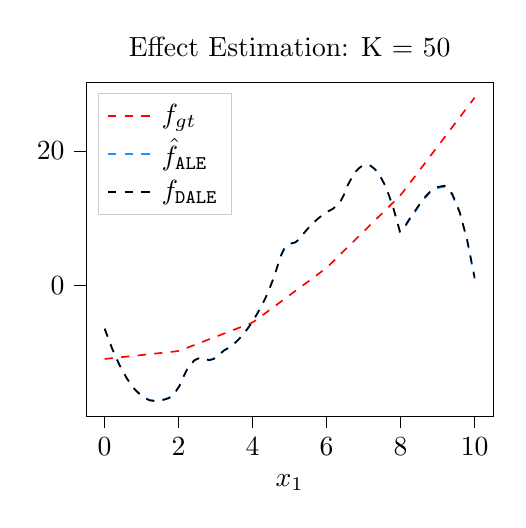
\begin{tikzpicture}

\definecolor{darkgray176}{RGB}{176,176,176}
\definecolor{dodgerblue}{RGB}{30,144,255}
\definecolor{lightgray204}{RGB}{204,204,204}

\begin{axis}[
legend cell align={left},
legend style={
  fill opacity=0.8,
  draw opacity=1,
  text opacity=1,
  at={(0.03,0.97)},
  anchor=north west,
  draw=lightgray204
},
tick align=outside,
tick pos=left,
title={Effect Estimation: K = 50},
x grid style={darkgray176},
xlabel={\(\displaystyle x_1\)},
xmin=-0.5, xmax=10.5,
xtick style={color=black},
y grid style={darkgray176},
ymin=-19.4760430884528, ymax=30.198088264309,
ytick style={color=black}
]
\addplot [semithick, red, dashed]
table {%
0 -10.9310787275426
0.101010101010101 -10.8718519947647
0.202020202020202 -10.8126252619868
0.303030303030303 -10.7533985292089
0.404040404040404 -10.6941717964309
0.505050505050505 -10.634945063653
0.606060606060606 -10.5757183308751
0.707070707070707 -10.5164915980972
0.808080808080808 -10.4572648653193
0.909090909090909 -10.3980381325414
1.01010101010101 -10.3388113997635
1.11111111111111 -10.2795846669856
1.21212121212121 -10.2203579342076
1.31313131313131 -10.1611312014297
1.41414141414141 -10.1019044686518
1.51515151515152 -10.0426777358739
1.61616161616162 -9.983451003096
1.71717171717172 -9.92422427031809
1.81818181818182 -9.86499753754018
1.91919191919192 -9.80577080476226
2.02020202020202 -9.71551411153251
2.12121212121212 -9.50113757649542
2.22222222222222 -9.28676104145832
2.32323232323232 -9.07238450642122
2.42424242424242 -8.85800797138412
2.52525252525253 -8.64363143634702
2.62626262626263 -8.42925490130992
2.72727272727273 -8.21487836627283
2.82828282828283 -8.00050183123573
2.92929292929293 -7.78612529619863
3.03030303030303 -7.57174876116153
3.13131313131313 -7.35737222612443
3.23232323232323 -7.14299569108734
3.33333333333333 -6.92861915605024
3.43434343434343 -6.71424262101314
3.53535353535354 -6.49986608597604
3.63636363636364 -6.28548955093894
3.73737373737374 -6.07111301590184
3.83838383838384 -5.85673648086475
3.93939393939394 -5.64235994582765
4.04040404040404 -5.34929709544007
4.14141414141414 -4.93820477202678
4.24242424242424 -4.52711244861348
4.34343434343434 -4.11602012520019
4.44444444444444 -3.70492780178689
4.54545454545454 -3.2938354783736
4.64646464646465 -2.8827431549603
4.74747474747475 -2.47165083154701
4.84848484848485 -2.06055850813371
4.94949494949495 -1.64946618472042
5.05050505050505 -1.23837386130712
5.15151515151515 -0.827281537893828
5.25252525252525 -0.416189214480532
5.35353535353535 -0.00509689106723599
5.45454545454545 0.405995432346057
5.55555555555556 0.817087755759353
5.65656565656566 1.22818007917265
5.75757575757576 1.63927240258595
5.85858585858586 2.05036472599924
5.95959595959596 2.46145704941253
6.06060606060606 2.95336271541685
6.16161616161616 3.49914394314852
6.26262626262626 4.04492517088019
6.36363636363636 4.59070639861185
6.46464646464646 5.13648762634352
6.56565656565657 5.68226885407519
6.66666666666667 6.22805008180686
6.76767676767677 6.77383130953853
6.86868686868687 7.3196125372702
6.96969696969697 7.86539376500187
7.07070707070707 8.41117499273354
7.17171717171717 8.9569562204652
7.27272727272727 9.50273744819687
7.37373737373737 10.0485186759285
7.47474747474747 10.5942999036602
7.57575757575758 11.1400811313919
7.67676767676768 11.6858623591235
7.77777777777778 12.2316435868552
7.87878787878788 12.7774248145869
7.97979797979798 13.3232060423185
8.08080808080808 14.0185364662469
8.18181818181818 14.7512541892244
8.28282828282828 15.4839719122019
8.38383838383838 16.2166896351795
8.48484848484848 16.949407358157
8.58585858585859 17.6821250811345
8.68686868686869 18.414842804112
8.78787878787879 19.1475605270896
8.88888888888889 19.8802782500671
8.98989898989899 20.6129959730446
9.09090909090909 21.3457136960221
9.19191919191919 22.0784314189997
9.29292929292929 22.8111491419772
9.39393939393939 23.5438668649547
9.49494949494949 24.2765845879322
9.5959595959596 25.0093023109097
9.6969696969697 25.7420200338873
9.7979797979798 26.4747377568648
9.8989898989899 27.2074554798423
10 27.9401732028198
};
\addlegendentry{$f_{gt}$}
\addplot [semithick, dodgerblue, dashed]
table {%
0 -6.39155669428798
0.101010101010101 -7.87176280822547
0.202020202020202 -9.34727774193452
0.303030303030303 -10.5929248444498
0.404040404040404 -11.8291895865083
0.505050505050505 -12.8402776776014
0.606060606060606 -13.8372922280092
0.707070707070707 -14.6138213076802
0.808080808080808 -15.3715856664374
0.909090909090909 -15.9135557346862
1.01010101010101 -16.4320699017928
1.11111111111111 -16.7394809586194
1.21212121212121 -17.0187449340754
1.31313131313131 -17.0915969794799
1.41414141414141 -17.1390709867376
1.51515151515152 -17.0306513310941
1.61616161616162 -16.9109325059248
1.71717171717172 -16.7318930407455
1.81818181818182 -16.4555098305769
1.91919191919192 -15.7356717821235
2.02020202020202 -14.9076740170153
2.12121212121212 -13.6470373852877
2.22222222222222 -12.4962403759351
2.32323232323232 -11.7348747550031
2.42424242424242 -11.093334176662
2.52525252525253 -10.8312395665255
2.62626262626263 -10.6989554191958
2.72727272727273 -10.9361318198549
2.82828282828283 -11.0627294254506
2.92929292929293 -10.9049815580264
3.03030303030303 -10.6345662571234
3.13131313131313 -10.1012602781034
3.23232323232323 -9.63635107348708
3.33333333333333 -9.31678501447877
3.43434343434343 -8.94376024612085
3.53535353535354 -8.46696268902541
3.63636363636364 -7.93356179261861
3.73737373737374 -7.29953273743605
3.83838383838384 -6.60575571298038
3.93939393939394 -5.81449515971068
4.04040404040404 -4.96034200720614
4.14141414141414 -4.01184995584932
4.24242424242424 -2.99732067529591
4.34343434343434 -1.89159712585195
4.44444444444444 -0.632456814122395
4.54545454545454 0.821941195061565
4.64646464646465 2.43672945572594
4.74747474747475 4.23980192464994
4.84848484848485 5.42690167554034
4.94949494949495 5.94669764856101
5.05050505050505 6.27649174108182
5.15151515151515 6.41628395310279
5.25252525252525 6.85742169129592
5.35353535353535 7.57672453057107
5.45454545454545 8.23871800219692
5.55555555555556 8.85189238286224
5.65656565656566 9.40563482670607
5.75757575757576 9.91268074876157
5.85858585858586 10.3581721648234
5.95959595959596 10.759089628269
6.06060606060606 11.0963300165488
6.16161616161616 11.3911190213847
6.26262626262626 11.8393282971996
6.36363636363636 12.3815693520016
6.46464646464646 13.4679123153837
6.56565656565657 14.8603126023421
6.66666666666667 15.932812724597
6.76767676767677 16.8405157923076
6.86868686868687 17.4186247509298
6.96969696969697 17.8416305993927
7.07070707070707 17.9253483943822
7.17171717171717 17.8636570235973
7.27272727272727 17.4443427206789
7.37373737373737 16.8859528330418
7.47474747474747 15.9600060429342
7.57575757575758 14.904917638445
7.67676767676768 13.4723383611482
7.77777777777778 11.9205514398069
7.87878787878788 9.98133967532086
7.97979797979798 7.93285423712737
8.08080808080808 8.30266103676541
8.18181818181818 9.27704089586134
8.28282828282828 10.104277296101
8.38383838383838 10.8992139126892
8.48484848484848 11.7249774233963
8.58585858585859 12.5566127234592
8.68686868686869 13.1768443933903
8.78787878787879 13.7626615188813
8.88888888888889 14.1321586507491
8.98989898989899 14.4721576016682
9.09090909090909 14.5909201954726
9.19191919191919 14.6851009718198
9.29292929292929 14.1088782566094
9.39393939393939 13.4743595856113
9.49494949494949 12.1548634341086
9.5959595959596 10.7916453157653
9.6969696969697 8.72887572797042
9.7979797979798 6.63695816228179
9.8989898989899 3.83091513819474
10 1.01029812516082
};
\addlegendentry{$\hat{f}_{\mathtt{ALE}}$}
\addplot [semithick, black, dashed]
table {%
0 -6.45366251536115
0.101010101010101 -7.93386862929863
0.202020202020202 -9.40939215334604
0.303030303030303 -10.6554687727793
0.404040404040404 -11.8921802124325
0.505050505050505 -12.9041273373615
0.606060606060606 -13.9020266926204
0.707070707070707 -14.6798443230453
0.808080808080808 -15.4389315939098
0.909090909090909 -15.9826197298305
1.01010101010101 -16.5028949163008
1.11111111111111 -16.8124535577173
1.21212121212121 -17.0939166597933
1.31313131313131 -17.1693458067056
1.41414141414141 -17.2181280269636
1.51515151515152 -17.1032219834882
1.61616161616162 -16.9773499822643
1.71717171717172 -16.7939067028611
1.81818181818182 -16.513516021749
1.91919191919192 -15.7914760661846
2.02020202020202 -14.961716775388
2.12121212121212 -13.7010801436624
2.22222222222222 -12.5502831343115
2.32323232323232 -11.7889175133799
2.42424242424242 -11.1473769350387
2.52525252525253 -10.885282324901
2.62626262626263 -10.7529981775697
2.72727272727273 -10.9901745782258
2.82828282828283 -11.1193372632691
2.92929292929293 -10.9707503938794
3.03030303030303 -10.6974283363254
3.13131313131313 -10.1330575063879
3.23232323232323 -9.64702420314582
3.33333333333333 -9.32745814413132
3.43434343434343 -8.9544333757688
3.53535353535354 -8.47763581867191
3.63636363636364 -7.94423492226536
3.73737373737374 -7.31020586708608
3.83838383838384 -6.61642884263549
3.93939393939394 -5.82516828937382
4.04040404040404 -4.9710151368792
4.14141414141414 -4.02252308553515
4.24242424242424 -3.00799380499648
4.34343434343434 -1.90227025557004
4.44444444444444 -0.643129943869416
4.54545454545454 0.811268065271056
4.64646464646465 2.42605632588
4.74747474747475 4.22912879473452
4.84848484848485 5.4163414868529
4.94949494949495 5.93637275417377
5.05050505050505 6.26617864414722
5.15151515151515 6.40575915677326
5.25252525252525 6.84679527925021
5.35353535353535 7.56609811851261
5.45454545454545 8.22809159012897
5.55555555555556 8.84126597078759
5.65656565656566 9.39500841462811
5.75757575757576 9.90205433668296
5.85858585858586 10.3475457527476
5.95959595959596 10.7484632161987
6.06060606060606 11.0857036044875
6.16161616161616 11.3804926093348
6.26262626262626 11.8288958481355
6.36363636363636 12.3714497464561
6.46464646464646 13.4606099564982
6.56565656565657 14.8572362168836
6.66666666666667 15.9330325984142
6.76767676767677 16.8435529817469
6.86868686868687 17.4235213686838
6.96969696969697 17.8479358749637
7.07070707070707 17.9320762673068
7.17171717171717 17.870384896534
7.27272727272727 17.4554824855752
7.37373737373737 16.9032202256552
7.47474747474747 15.9879355077662
7.57575757575758 14.945102358699
7.67676767676768 13.5294353338799
7.77777777777778 11.9960312956654
7.87878787878788 10.0799819639161
7.97979797979798 8.05600703655439
8.08080808080808 8.43976704288982
8.18181818181818 9.42546078264953
8.28282828282828 10.2583595903086
8.38383838383838 11.0577180470188
8.48484848484848 11.8841890521459
8.58585858585859 12.7158243522095
8.68686868686869 13.3360560221302
8.78787878787879 13.9218731476089
8.88888888888889 14.291370279453
8.98989898989899 14.6313692303469
9.09090909090909 14.7501318241145
9.19191919191919 14.8443126004235
9.29292929292929 14.2680899176152
9.39393939393939 13.6335712818401
9.49494949494949 12.3140751987059
9.5959595959596 10.9508571508466
9.6969696969697 8.88808766738661
9.7979797979798 6.79617020744323
9.8989898989899 3.99012732365734
10 1.16951045162982
};
\addlegendentry{$f_{\mathtt{DALE}}$}
\end{axis}

\end{tikzpicture}
}
    \resizebox{.32\columnwidth}{!}{% This file was created with tikzplotlib v0.10.1.
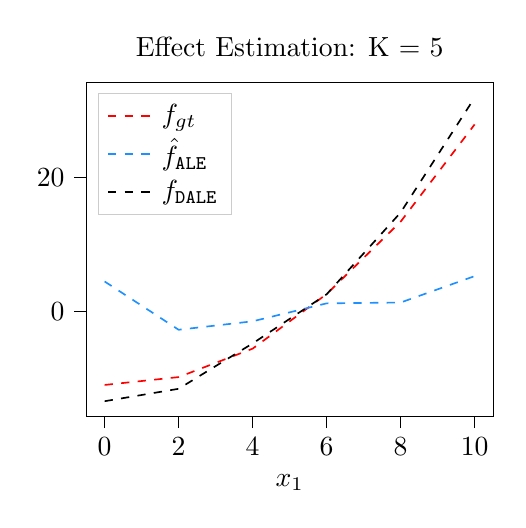
\begin{tikzpicture}

\definecolor{darkgray176}{RGB}{176,176,176}
\definecolor{dodgerblue}{RGB}{30,144,255}
\definecolor{lightgray204}{RGB}{204,204,204}

\begin{axis}[
legend cell align={left},
legend style={
  fill opacity=0.8,
  draw opacity=1,
  text opacity=1,
  at={(0.03,0.97)},
  anchor=north west,
  draw=lightgray204
},
tick align=outside,
tick pos=left,
title={Effect Estimation: K = 5},
x grid style={darkgray176},
xlabel={\(\displaystyle x_1\)},
xmin=-0.5, xmax=10.5,
xtick style={color=black},
y grid style={darkgray176},
ymin=-15.623228566917, ymax=34.2007169448902,
ytick style={color=black}
]
\addplot [semithick, red, dashed]
table {%
0 -10.9310787275426
0.01001001001001 -10.9252094116817
0.02002002002002 -10.9193400958208
0.03003003003003 -10.91347077996
0.04004004004004 -10.9076014640991
0.05005005005005 -10.9017321482382
0.0600600600600601 -10.8958628323774
0.0700700700700701 -10.8899935165165
0.0800800800800801 -10.8841242006556
0.0900900900900901 -10.8782548847947
0.1001001001001 -10.8723855689339
0.11011011011011 -10.866516253073
0.12012012012012 -10.8606469372121
0.13013013013013 -10.8547776213512
0.14014014014014 -10.8489083054904
0.15015015015015 -10.8430389896295
0.16016016016016 -10.8371696737686
0.17017017017017 -10.8313003579077
0.18018018018018 -10.8254310420469
0.19019019019019 -10.819561726186
0.2002002002002 -10.8136924103251
0.21021021021021 -10.8078230944642
0.22022022022022 -10.8019537786034
0.23023023023023 -10.7960844627425
0.24024024024024 -10.7902151468816
0.25025025025025 -10.7843458310207
0.26026026026026 -10.7784765151599
0.27027027027027 -10.772607199299
0.28028028028028 -10.7667378834381
0.29029029029029 -10.7608685675772
0.3003003003003 -10.7549992517164
0.31031031031031 -10.7491299358555
0.32032032032032 -10.7432606199946
0.33033033033033 -10.7373913041337
0.34034034034034 -10.7315219882729
0.35035035035035 -10.725652672412
0.36036036036036 -10.7197833565511
0.37037037037037 -10.7139140406903
0.38038038038038 -10.7080447248294
0.39039039039039 -10.7021754089685
0.4004004004004 -10.6963060931076
0.41041041041041 -10.6904367772468
0.42042042042042 -10.6845674613859
0.43043043043043 -10.678698145525
0.44044044044044 -10.6728288296641
0.45045045045045 -10.6669595138033
0.46046046046046 -10.6610901979424
0.47047047047047 -10.6552208820815
0.48048048048048 -10.6493515662206
0.49049049049049 -10.6434822503598
0.500500500500501 -10.6376129344989
0.510510510510511 -10.631743618638
0.520520520520521 -10.6258743027771
0.530530530530531 -10.6200049869163
0.540540540540541 -10.6141356710554
0.550550550550551 -10.6082663551945
0.560560560560561 -10.6023970393336
0.570570570570571 -10.5965277234728
0.580580580580581 -10.5906584076119
0.590590590590591 -10.584789091751
0.600600600600601 -10.5789197758901
0.610610610610611 -10.5730504600293
0.620620620620621 -10.5671811441684
0.630630630630631 -10.5613118283075
0.640640640640641 -10.5554425124466
0.650650650650651 -10.5495731965858
0.660660660660661 -10.5437038807249
0.670670670670671 -10.537834564864
0.680680680680681 -10.5319652490032
0.690690690690691 -10.5260959331423
0.700700700700701 -10.5202266172814
0.710710710710711 -10.5143573014205
0.720720720720721 -10.5084879855597
0.730730730730731 -10.5026186696988
0.740740740740741 -10.4967493538379
0.750750750750751 -10.490880037977
0.760760760760761 -10.4850107221162
0.770770770770771 -10.4791414062553
0.780780780780781 -10.4732720903944
0.790790790790791 -10.4674027745335
0.800800800800801 -10.4615334586727
0.810810810810811 -10.4556641428118
0.820820820820821 -10.4497948269509
0.830830830830831 -10.44392551109
0.840840840840841 -10.4380561952292
0.850850850850851 -10.4321868793683
0.860860860860861 -10.4263175635074
0.870870870870871 -10.4204482476465
0.880880880880881 -10.4145789317857
0.890890890890891 -10.4087096159248
0.900900900900901 -10.4028403000639
0.910910910910911 -10.396970984203
0.920920920920921 -10.3911016683422
0.930930930930931 -10.3852323524813
0.940940940940941 -10.3793630366204
0.950950950950951 -10.3734937207595
0.960960960960961 -10.3676244048987
0.970970970970971 -10.3617550890378
0.980980980980981 -10.3558857731769
0.990990990990991 -10.3500164573161
1.001001001001 -10.3441471414552
1.01101101101101 -10.3382778255943
1.02102102102102 -10.3324085097334
1.03103103103103 -10.3265391938726
1.04104104104104 -10.3206698780117
1.05105105105105 -10.3148005621508
1.06106106106106 -10.3089312462899
1.07107107107107 -10.3030619304291
1.08108108108108 -10.2971926145682
1.09109109109109 -10.2913232987073
1.1011011011011 -10.2854539828464
1.11111111111111 -10.2795846669856
1.12112112112112 -10.2737153511247
1.13113113113113 -10.2678460352638
1.14114114114114 -10.2619767194029
1.15115115115115 -10.2561074035421
1.16116116116116 -10.2502380876812
1.17117117117117 -10.2443687718203
1.18118118118118 -10.2384994559594
1.19119119119119 -10.2326301400986
1.2012012012012 -10.2267608242377
1.21121121121121 -10.2208915083768
1.22122122122122 -10.2150221925159
1.23123123123123 -10.2091528766551
1.24124124124124 -10.2032835607942
1.25125125125125 -10.1974142449333
1.26126126126126 -10.1915449290724
1.27127127127127 -10.1856756132116
1.28128128128128 -10.1798062973507
1.29129129129129 -10.1739369814898
1.3013013013013 -10.168067665629
1.31131131131131 -10.1621983497681
1.32132132132132 -10.1563290339072
1.33133133133133 -10.1504597180463
1.34134134134134 -10.1445904021855
1.35135135135135 -10.1387210863246
1.36136136136136 -10.1328517704637
1.37137137137137 -10.1269824546028
1.38138138138138 -10.121113138742
1.39139139139139 -10.1152438228811
1.4014014014014 -10.1093745070202
1.41141141141141 -10.1035051911593
1.42142142142142 -10.0976358752985
1.43143143143143 -10.0917665594376
1.44144144144144 -10.0858972435767
1.45145145145145 -10.0800279277158
1.46146146146146 -10.074158611855
1.47147147147147 -10.0682892959941
1.48148148148148 -10.0624199801332
1.49149149149149 -10.0565506642723
1.5015015015015 -10.0506813484115
1.51151151151151 -10.0448120325506
1.52152152152152 -10.0389427166897
1.53153153153153 -10.0330734008288
1.54154154154154 -10.027204084968
1.55155155155155 -10.0213347691071
1.56156156156156 -10.0154654532462
1.57157157157157 -10.0095961373853
1.58158158158158 -10.0037268215245
1.59159159159159 -9.9978575056636
1.6016016016016 -9.99198818980273
1.61161161161161 -9.98611887394185
1.62162162162162 -9.98024955808098
1.63163163163163 -9.9743802422201
1.64164164164164 -9.96851092635923
1.65165165165165 -9.96264161049836
1.66166166166166 -9.95677229463748
1.67167167167167 -9.95090297877661
1.68168168168168 -9.94503366291573
1.69169169169169 -9.93916434705486
1.7017017017017 -9.93329503119399
1.71171171171171 -9.92742571533311
1.72172172172172 -9.92155639947224
1.73173173173173 -9.91568708361136
1.74174174174174 -9.90981776775049
1.75175175175175 -9.90394845188961
1.76176176176176 -9.89807913602874
1.77177177177177 -9.89220982016787
1.78178178178178 -9.88634050430699
1.79179179179179 -9.88047118844612
1.8018018018018 -9.87460187258524
1.81181181181181 -9.86873255672437
1.82182182182182 -9.86286324086349
1.83183183183183 -9.85699392500262
1.84184184184184 -9.85112460914175
1.85185185185185 -9.84525529328087
1.86186186186186 -9.83938597742
1.87187187187187 -9.83351666155912
1.88188188188188 -9.82764734569825
1.89189189189189 -9.82177802983738
1.9019019019019 -9.8159087139765
1.91191191191191 -9.81003939811563
1.92192192192192 -9.80417008225475
1.93193193193193 -9.79830076639388
1.94194194194194 -9.792431450533
1.95195195195195 -9.78656213467213
1.96196196196196 -9.78069281881126
1.97197197197197 -9.77482350295038
1.98198198198198 -9.76895418708951
1.99199199199199 -9.76308487122863
2.002002002002 -9.7541405142419
2.01201201201201 -9.73289599275174
2.02202202202202 -9.71165147126158
2.03203203203203 -9.69040694977141
2.04204204204204 -9.66916242828125
2.05205205205205 -9.64791790679109
2.06206206206206 -9.62667338530092
2.07207207207207 -9.60542886381076
2.08208208208208 -9.5841843423206
2.09209209209209 -9.56293982083043
2.1021021021021 -9.54169529934027
2.11211211211211 -9.52045077785011
2.12212212212212 -9.49920625635995
2.13213213213213 -9.47796173486978
2.14214214214214 -9.45671721337962
2.15215215215215 -9.43547269188946
2.16216216216216 -9.41422817039929
2.17217217217217 -9.39298364890913
2.18218218218218 -9.37173912741897
2.19219219219219 -9.35049460592881
2.2022022022022 -9.32925008443864
2.21221221221221 -9.30800556294848
2.22222222222222 -9.28676104145832
2.23223223223223 -9.26551651996815
2.24224224224224 -9.24427199847799
2.25225225225225 -9.22302747698783
2.26226226226226 -9.20178295549767
2.27227227227227 -9.1805384340075
2.28228228228228 -9.15929391251734
2.29229229229229 -9.13804939102718
2.3023023023023 -9.11680486953701
2.31231231231231 -9.09556034804685
2.32232232232232 -9.07431582655669
2.33233233233233 -9.05307130506653
2.34234234234234 -9.03182678357636
2.35235235235235 -9.0105822620862
2.36236236236236 -8.98933774059604
2.37237237237237 -8.96809321910587
2.38238238238238 -8.94684869761571
2.39239239239239 -8.92560417612555
2.4024024024024 -8.90435965463539
2.41241241241241 -8.88311513314522
2.42242242242242 -8.86187061165506
2.43243243243243 -8.8406260901649
2.44244244244244 -8.81938156867473
2.45245245245245 -8.79813704718457
2.46246246246246 -8.77689252569441
2.47247247247247 -8.75564800420425
2.48248248248248 -8.73440348271408
2.49249249249249 -8.71315896122392
2.5025025025025 -8.69191443973376
2.51251251251251 -8.67066991824359
2.52252252252252 -8.64942539675343
2.53253253253253 -8.62818087526327
2.54254254254254 -8.6069363537731
2.55255255255255 -8.58569183228294
2.56256256256256 -8.56444731079278
2.57257257257257 -8.54320278930262
2.58258258258258 -8.52195826781245
2.59259259259259 -8.50071374632229
2.6026026026026 -8.47946922483213
2.61261261261261 -8.45822470334197
2.62262262262262 -8.4369801818518
2.63263263263263 -8.41573566036164
2.64264264264264 -8.39449113887148
2.65265265265265 -8.37324661738131
2.66266266266266 -8.35200209589115
2.67267267267267 -8.33075757440099
2.68268268268268 -8.30951305291082
2.69269269269269 -8.28826853142066
2.7027027027027 -8.2670240099305
2.71271271271271 -8.24577948844034
2.72272272272272 -8.22453496695017
2.73273273273273 -8.20329044546001
2.74274274274274 -8.18204592396985
2.75275275275275 -8.16080140247968
2.76276276276276 -8.13955688098952
2.77277277277277 -8.11831235949936
2.78278278278278 -8.0970678380092
2.79279279279279 -8.07582331651903
2.8028028028028 -8.05457879502887
2.81281281281281 -8.03333427353871
2.82282282282282 -8.01208975204855
2.83283283283283 -7.99084523055838
2.84284284284284 -7.96960070906822
2.85285285285285 -7.94835618757806
2.86286286286286 -7.92711166608789
2.87287287287287 -7.90586714459773
2.88288288288288 -7.88462262310757
2.89289289289289 -7.8633781016174
2.9029029029029 -7.84213358012724
2.91291291291291 -7.82088905863708
2.92292292292292 -7.79964453714692
2.93293293293293 -7.77840001565675
2.94294294294294 -7.75715549416659
2.95295295295295 -7.73591097267643
2.96296296296296 -7.71466645118626
2.97297297297297 -7.6934219296961
2.98298298298298 -7.67217740820594
2.99299299299299 -7.65093288671578
3.003003003003 -7.62968836522561
3.01301301301301 -7.60844384373545
3.02302302302302 -7.58719932224529
3.03303303303303 -7.56595480075512
3.04304304304304 -7.54471027926496
3.05305305305305 -7.5234657577748
3.06306306306306 -7.50222123628463
3.07307307307307 -7.48097671479447
3.08308308308308 -7.45973219330431
3.09309309309309 -7.43848767181415
3.1031031031031 -7.41724315032398
3.11311311311311 -7.39599862883382
3.12312312312312 -7.37475410734366
3.13313313313313 -7.3535095858535
3.14314314314314 -7.33226506436333
3.15315315315315 -7.31102054287317
3.16316316316316 -7.28977602138301
3.17317317317317 -7.26853149989284
3.18318318318318 -7.24728697840268
3.19319319319319 -7.22604245691252
3.2032032032032 -7.20479793542236
3.21321321321321 -7.18355341393219
3.22322322322322 -7.16230889244203
3.23323323323323 -7.14106437095187
3.24324324324324 -7.1198198494617
3.25325325325325 -7.09857532797154
3.26326326326326 -7.07733080648138
3.27327327327327 -7.05608628499121
3.28328328328328 -7.03484176350105
3.29329329329329 -7.01359724201089
3.3033033033033 -6.99235272052073
3.31331331331331 -6.97110819903056
3.32332332332332 -6.9498636775404
3.33333333333333 -6.92861915605024
3.34334334334334 -6.90737463456007
3.35335335335335 -6.88613011306991
3.36336336336336 -6.86488559157975
3.37337337337337 -6.84364107008959
3.38338338338338 -6.82239654859942
3.39339339339339 -6.80115202710926
3.4034034034034 -6.7799075056191
3.41341341341341 -6.75866298412893
3.42342342342342 -6.73741846263877
3.43343343343343 -6.71617394114861
3.44344344344344 -6.69492941965845
3.45345345345345 -6.67368489816828
3.46346346346346 -6.65244037667812
3.47347347347347 -6.63119585518796
3.48348348348348 -6.60995133369779
3.49349349349349 -6.58870681220763
3.5035035035035 -6.56746229071747
3.51351351351351 -6.54621776922731
3.52352352352352 -6.52497324773714
3.53353353353353 -6.50372872624698
3.54354354354354 -6.48248420475682
3.55355355355355 -6.46123968326665
3.56356356356356 -6.43999516177649
3.57357357357357 -6.41875064028633
3.58358358358358 -6.39750611879617
3.59359359359359 -6.376261597306
3.6036036036036 -6.35501707581584
3.61361361361361 -6.33377255432568
3.62362362362362 -6.31252803283551
3.63363363363363 -6.29128351134535
3.64364364364364 -6.27003898985519
3.65365365365365 -6.24879446836503
3.66366366366366 -6.22754994687486
3.67367367367367 -6.2063054253847
3.68368368368368 -6.18506090389454
3.69369369369369 -6.16381638240437
3.7037037037037 -6.14257186091421
3.71371371371371 -6.12132733942405
3.72372372372372 -6.10008281793388
3.73373373373373 -6.07883829644372
3.74374374374374 -6.05759377495356
3.75375375375375 -6.0363492534634
3.76376376376376 -6.01510473197323
3.77377377377377 -5.99386021048307
3.78378378378378 -5.97261568899291
3.79379379379379 -5.95137116750274
3.8038038038038 -5.93012664601258
3.81381381381381 -5.90888212452242
3.82382382382382 -5.88763760303226
3.83383383383383 -5.86639308154209
3.84384384384384 -5.84514856005193
3.85385385385385 -5.82390403856177
3.86386386386386 -5.8026595170716
3.87387387387387 -5.78141499558144
3.88388388388388 -5.76017047409128
3.89389389389389 -5.73892595260112
3.9039039039039 -5.71768143111095
3.91391391391391 -5.69643690962079
3.92392392392392 -5.67519238813063
3.93393393393393 -5.65394786664046
3.94394394394394 -5.6327033451503
3.95395395395395 -5.61145882366014
3.96396396396396 -5.59021430216998
3.97397397397397 -5.56896978067981
3.98398398398398 -5.54772525918965
3.99399399399399 -5.52648073769949
4.004004004004 -5.49743847324666
4.01401401401401 -5.45669959434985
4.02402402402402 -5.41596071545304
4.03403403403403 -5.37522183655622
4.04404404404404 -5.33448295765941
4.05405405405405 -5.2937440787626
4.06406406406406 -5.25300519986578
4.07407407407407 -5.21226632096897
4.08408408408408 -5.17152744207216
4.09409409409409 -5.13078856317535
4.1041041041041 -5.09004968427853
4.11411411411411 -5.04931080538172
4.12412412412412 -5.00857192648491
4.13413413413413 -4.96783304758809
4.14414414414414 -4.92709416869128
4.15415415415415 -4.88635528979447
4.16416416416416 -4.84561641089765
4.17417417417417 -4.80487753200084
4.18418418418418 -4.76413865310403
4.19419419419419 -4.72339977420722
4.2042042042042 -4.6826608953104
4.21421421421421 -4.64192201641359
4.22422422422422 -4.60118313751678
4.23423423423423 -4.56044425861996
4.24424424424424 -4.51970537972315
4.25425425425425 -4.47896650082634
4.26426426426426 -4.43822762192952
4.27427427427427 -4.39748874303271
4.28428428428428 -4.3567498641359
4.29429429429429 -4.31601098523909
4.3043043043043 -4.27527210634227
4.31431431431431 -4.23453322744546
4.32432432432432 -4.19379434854865
4.33433433433433 -4.15305546965183
4.34434434434434 -4.11231659075502
4.35435435435435 -4.07157771185821
4.36436436436436 -4.03083883296139
4.37437437437437 -3.99009995406458
4.38438438438438 -3.94936107516777
4.39439439439439 -3.90862219627096
4.4044044044044 -3.86788331737414
4.41441441441441 -3.82714443847733
4.42442442442442 -3.78640555958052
4.43443443443443 -3.7456666806837
4.44444444444444 -3.70492780178689
4.45445445445445 -3.66418892289008
4.46446446446446 -3.62345004399326
4.47447447447447 -3.58271116509645
4.48448448448448 -3.54197228619964
4.49449449449449 -3.50123340730283
4.5045045045045 -3.46049452840601
4.51451451451451 -3.4197556495092
4.52452452452452 -3.37901677061239
4.53453453453453 -3.33827789171557
4.54454454454454 -3.29753901281876
4.55455455455455 -3.25680013392195
4.56456456456456 -3.21606125502514
4.57457457457457 -3.17532237612832
4.58458458458458 -3.13458349723151
4.59459459459459 -3.0938446183347
4.6046046046046 -3.05310573943788
4.61461461461461 -3.01236686054107
4.62462462462462 -2.97162798164426
4.63463463463463 -2.93088910274744
4.64464464464464 -2.89015022385063
4.65465465465465 -2.84941134495382
4.66466466466466 -2.808672466057
4.67467467467467 -2.76793358716019
4.68468468468468 -2.72719470826338
4.69469469469469 -2.68645582936657
4.7047047047047 -2.64571695046975
4.71471471471471 -2.60497807157294
4.72472472472472 -2.56423919267613
4.73473473473473 -2.52350031377931
4.74474474474474 -2.4827614348825
4.75475475475475 -2.44202255598569
4.76476476476476 -2.40128367708888
4.77477477477477 -2.36054479819206
4.78478478478478 -2.31980591929525
4.79479479479479 -2.27906704039844
4.8048048048048 -2.23832816150162
4.81481481481481 -2.19758928260481
4.82482482482482 -2.156850403708
4.83483483483483 -2.11611152481118
4.84484484484484 -2.07537264591437
4.85485485485485 -2.03463376701756
4.86486486486486 -1.99389488812074
4.87487487487487 -1.95315600922393
4.88488488488488 -1.91241713032712
4.89489489489489 -1.87167825143031
4.9049049049049 -1.83093937253349
4.91491491491491 -1.79020049363668
4.92492492492492 -1.74946161473987
4.93493493493493 -1.70872273584305
4.94494494494494 -1.66798385694624
4.95495495495495 -1.62724497804943
4.96496496496496 -1.58650609915261
4.97497497497497 -1.5457672202558
4.98498498498498 -1.50502834135899
4.99499499499499 -1.46428946246218
5.00500500500501 -1.42355058356536
5.01501501501502 -1.38281170466855
5.02502502502503 -1.34207282577174
5.03503503503504 -1.30133394687492
5.04504504504505 -1.26059506797811
5.05505505505506 -1.2198561890813
5.06506506506507 -1.17911731018448
5.07507507507508 -1.13837843128767
5.08508508508509 -1.09763955239086
5.0950950950951 -1.05690067349405
5.10510510510511 -1.01616179459723
5.11511511511512 -0.97542291570042
5.12512512512513 -0.934684036803606
5.13513513513514 -0.893945157906794
5.14514514514515 -0.853206279009981
5.15515515515516 -0.812467400113167
5.16516516516517 -0.771728521216353
5.17517517517518 -0.730989642319543
5.18518518518519 -0.690250763422728
5.1951951951952 -0.649511884525914
5.20520520520521 -0.608773005629104
5.21521521521522 -0.568034126732289
5.22522522522523 -0.527295247835475
5.23523523523524 -0.486556368938665
5.24524524524525 -0.445817490041851
5.25525525525526 -0.405078611145036
5.26526526526527 -0.364339732248224
5.27527527527528 -0.323600853351412
5.28528528528529 -0.282861974454597
5.2952952952953 -0.242123095557785
5.30530530530531 -0.201384216660973
5.31531531531532 -0.160645337764159
5.32532532532533 -0.119906458867346
5.33533533533534 -0.0791675799705338
5.34534534534535 -0.0384287010737197
5.35535535535536 0.00231017782309273
5.36536536536537 0.0430490567199051
5.37537537537538 0.0837879356167193
5.38538538538539 0.124526814513532
5.3953953953954 0.165265693410344
5.40540540540541 0.206004572307158
5.41541541541542 0.246743451203971
5.42542542542543 0.287482330100783
5.43543543543544 0.328221208997597
5.44544544544545 0.368960087894409
5.45545545545546 0.409698966791222
5.46546546546547 0.450437845688036
5.47547547547548 0.491176724584848
5.48548548548549 0.531915603481661
5.4954954954955 0.572654482378475
5.50550550550551 0.613393361275287
5.51551551551552 0.6541322401721
5.52552552552553 0.694871119068914
5.53553553553554 0.735609997965726
5.54554554554555 0.776348876862539
5.55555555555556 0.817087755759353
5.56556556556557 0.857826634656165
5.57557557557558 0.898565513552978
5.58558558558559 0.939304392449792
5.5955955955956 0.980043271346606
5.60560560560561 1.02078215024342
5.61561561561562 1.06152102914023
5.62562562562563 1.10225990803704
5.63563563563564 1.14299878693386
5.64564564564565 1.18373766583067
5.65565565565566 1.22447654472748
5.66566566566567 1.26521542362429
5.67567567567568 1.30595430252111
5.68568568568569 1.34669318141792
5.6956956956957 1.38743206031473
5.70570570570571 1.42817093921155
5.71571571571572 1.46890981810836
5.72572572572573 1.50964869700517
5.73573573573574 1.55038757590199
5.74574574574575 1.5911264547988
5.75575575575576 1.63186533369561
5.76576576576577 1.67260421259243
5.77577577577578 1.71334309148924
5.78578578578579 1.75408197038605
5.7957957957958 1.79482084928286
5.80580580580581 1.83555972817968
5.81581581581582 1.87629860707649
5.82582582582583 1.9170374859733
5.83583583583584 1.95777636487012
5.84584584584585 1.99851524376693
5.85585585585586 2.03925412266374
5.86586586586587 2.07999300156056
5.87587587587588 2.12073188045737
5.88588588588589 2.16147075935418
5.8958958958959 2.202209638251
5.90590590590591 2.24294851714781
5.91591591591592 2.28368739604462
5.92592592592593 2.32442627494143
5.93593593593594 2.36516515383825
5.94594594594595 2.40590403273506
5.95595595595596 2.44664291163187
5.96596596596597 2.48738179052869
5.97597597597598 2.5281206694255
5.98598598598599 2.56885954832231
5.995995995996 2.60959842721912
6.00600600600601 2.65834583556189
6.01601601601602 2.7124322635353
6.02602602602603 2.76651869150871
6.03603603603604 2.82060511948212
6.04604604604605 2.87469154745553
6.05605605605606 2.92877797542894
6.06606606606607 2.98286440340235
6.07607607607608 3.03695083137575
6.08608608608609 3.09103725934916
6.0960960960961 3.14512368732257
6.10610610610611 3.19921011529598
6.11611611611612 3.25329654326939
6.12612612612613 3.3073829712428
6.13613613613614 3.3614693992162
6.14614614614615 3.41555582718961
6.15615615615616 3.46964225516302
6.16616616616617 3.52372868313643
6.17617617617618 3.57781511110984
6.18618618618619 3.63190153908325
6.1961961961962 3.68598796705666
6.20620620620621 3.74007439503007
6.21621621621622 3.79416082300347
6.22622622622623 3.84824725097688
6.23623623623624 3.90233367895029
6.24624624624625 3.9564201069237
6.25625625625626 4.01050653489711
6.26626626626627 4.06459296287052
6.27627627627628 4.11867939084392
6.28628628628629 4.17276581881733
6.2962962962963 4.22685224679074
6.30630630630631 4.28093867476415
6.31631631631632 4.33502510273756
6.32632632632633 4.38911153071097
6.33633633633634 4.44319795868438
6.34634634634635 4.49728438665778
6.35635635635636 4.55137081463119
6.36636636636637 4.6054572426046
6.37637637637638 4.65954367057801
6.38638638638639 4.71363009855142
6.3963963963964 4.76771652652483
6.40640640640641 4.82180295449824
6.41641641641642 4.87588938247165
6.42642642642643 4.92997581044506
6.43643643643644 4.98406223841847
6.44644644644645 5.03814866639187
6.45645645645646 5.09223509436528
6.46646646646647 5.14632152233869
6.47647647647648 5.2004079503121
6.48648648648649 5.25449437828551
6.4964964964965 5.30858080625892
6.50650650650651 5.36266723423233
6.51651651651652 5.41675366220574
6.52652652652653 5.47084009017914
6.53653653653654 5.52492651815255
6.54654654654655 5.57901294612596
6.55655655655656 5.63309937409937
6.56656656656657 5.68718580207278
6.57657657657658 5.74127223004619
6.58658658658659 5.79535865801959
6.5965965965966 5.849445085993
6.60660660660661 5.90353151396641
6.61661661661662 5.95761794193982
6.62662662662663 6.01170436991323
6.63663663663664 6.06579079788663
6.64664664664665 6.11987722586004
6.65665665665666 6.17396365383345
6.66666666666667 6.22805008180686
6.67667667667668 6.28213650978027
6.68668668668669 6.33622293775368
6.6966966966967 6.39030936572709
6.70670670670671 6.4443957937005
6.71671671671672 6.4984822216739
6.72672672672673 6.55256864964731
6.73673673673674 6.60665507762072
6.74674674674675 6.66074150559413
6.75675675675676 6.71482793356754
6.76676676676677 6.76891436154095
6.77677677677678 6.82300078951436
6.78678678678679 6.87708721748776
6.7967967967968 6.93117364546117
6.80680680680681 6.98526007343458
6.81681681681682 7.03934650140799
6.82682682682683 7.0934329293814
6.83683683683684 7.14751935735481
6.84684684684685 7.20160578532822
6.85685685685686 7.25569221330163
6.86686686686687 7.30977864127503
6.87687687687688 7.36386506924844
6.88688688688689 7.41795149722185
6.8968968968969 7.47203792519526
6.90690690690691 7.52612435316867
6.91691691691692 7.58021078114207
6.92692692692693 7.63429720911548
6.93693693693694 7.68838363708889
6.94694694694695 7.7424700650623
6.95695695695696 7.79655649303571
6.96696696696697 7.85064292100912
6.97697697697698 7.90472934898253
6.98698698698699 7.95881577695593
6.996996996997 8.01290220492934
7.00700700700701 8.06698863290275
7.01701701701702 8.12107506087616
7.02702702702703 8.17516148884957
7.03703703703704 8.22924791682298
7.04704704704705 8.28333434479639
7.05705705705706 8.33742077276979
7.06706706706707 8.3915072007432
7.07707707707708 8.44559362871661
7.08708708708709 8.49968005669002
7.0970970970971 8.55376648466343
7.10710710710711 8.60785291263684
7.11711711711712 8.66193934061025
7.12712712712713 8.71602576858366
7.13713713713714 8.77011219655706
7.14714714714715 8.82419862453047
7.15715715715716 8.87828505250388
7.16716716716717 8.93237148047729
7.17717717717718 8.9864579084507
7.18718718718719 9.04054433642411
7.1971971971972 9.09463076439751
7.20720720720721 9.14871719237092
7.21721721721722 9.20280362034433
7.22722722722723 9.25689004831774
7.23723723723724 9.31097647629115
7.24724724724725 9.36506290426455
7.25725725725726 9.41914933223796
7.26726726726727 9.47323576021137
7.27727727727728 9.52732218818478
7.28728728728729 9.58140861615819
7.2972972972973 9.6354950441316
7.30730730730731 9.68958147210501
7.31731731731732 9.74366790007841
7.32732732732733 9.79775432805182
7.33733733733734 9.85184075602523
7.34734734734735 9.90592718399864
7.35735735735736 9.96001361197205
7.36736736736737 10.0141000399455
7.37737737737738 10.0681864679189
7.38738738738739 10.1222728958923
7.3973973973974 10.1763593238657
7.40740740740741 10.2304457518391
7.41741741741742 10.2845321798125
7.42742742742743 10.3386186077859
7.43743743743744 10.3927050357593
7.44744744744745 10.4467914637327
7.45745745745746 10.5008778917061
7.46746746746747 10.5549643196795
7.47747747747748 10.609050747653
7.48748748748749 10.6631371756264
7.4974974974975 10.7172236035998
7.50750750750751 10.7713100315732
7.51751751751752 10.8253964595466
7.52752752752753 10.87948288752
7.53753753753754 10.9335693154934
7.54754754754755 10.9876557434668
7.55755755755756 11.0417421714402
7.56756756756757 11.0958285994136
7.57757757757758 11.149915027387
7.58758758758759 11.2040014553604
7.5975975975976 11.2580878833339
7.60760760760761 11.3121743113073
7.61761761761762 11.3662607392807
7.62762762762763 11.4203471672541
7.63763763763764 11.4744335952275
7.64764764764765 11.5285200232009
7.65765765765766 11.5826064511743
7.66766766766767 11.6366928791477
7.67767767767768 11.6907793071211
7.68768768768769 11.7448657350945
7.6976976976977 11.7989521630679
7.70770770770771 11.8530385910413
7.71771771771772 11.9071250190148
7.72772772772773 11.9612114469882
7.73773773773774 12.0152978749616
7.74774774774775 12.069384302935
7.75775775775776 12.1234707309084
7.76776776776777 12.1775571588818
7.77777777777778 12.2316435868552
7.78778778778779 12.2857300148286
7.7977977977978 12.339816442802
7.80780780780781 12.3939028707754
7.81781781781782 12.4479892987488
7.82782782782783 12.5020757267222
7.83783783783784 12.5561621546957
7.84784784784785 12.6102485826691
7.85785785785786 12.6643350106425
7.86786786786787 12.7184214386159
7.87787787787788 12.7725078665893
7.88788788788789 12.8265942945627
7.8978978978979 12.8806807225361
7.90790790790791 12.9347671505095
7.91791791791792 12.9888535784829
7.92792792792793 13.0429400064563
7.93793793793794 13.0970264344297
7.94794794794795 13.1511128624032
7.95795795795796 13.2051992903766
7.96796796796797 13.25928571835
7.97797797797798 13.3133721463234
7.98798798798799 13.3674585742968
7.997997997998 13.4215450022702
8.00800800800801 13.4904516208577
8.01801801801802 13.5630632870987
8.02802802802803 13.6356749533397
8.03803803803804 13.7082866195807
8.04804804804805 13.7808982858218
8.05805805805806 13.8535099520628
8.06806806806807 13.9261216183038
8.07807807807808 13.9987332845448
8.08808808808809 14.0713449507858
8.0980980980981 14.1439566170268
8.10810810810811 14.2165682832679
8.11811811811812 14.2891799495089
8.12812812812813 14.3617916157499
8.13813813813814 14.4344032819909
8.14814814814815 14.5070149482319
8.15815815815816 14.5796266144729
8.16816816816817 14.6522382807139
8.17817817817818 14.724849946955
8.18818818818819 14.797461613196
8.1981981981982 14.870073279437
8.20820820820821 14.942684945678
8.21821821821822 15.015296611919
8.22822822822823 15.08790827816
8.23823823823824 15.1605199444011
8.24824824824825 15.2331316106421
8.25825825825826 15.3057432768831
8.26826826826827 15.3783549431241
8.27827827827828 15.4509666093651
8.28828828828829 15.5235782756061
8.2982982982983 15.5961899418472
8.30830830830831 15.6688016080882
8.31831831831832 15.7414132743292
8.32832832832833 15.8140249405702
8.33833833833834 15.8866366068112
8.34834834834835 15.9592482730522
8.35835835835836 16.0318599392932
8.36836836836837 16.1044716055343
8.37837837837838 16.1770832717753
8.38838838838839 16.2496949380163
8.3983983983984 16.3223066042573
8.40840840840841 16.3949182704983
8.41841841841842 16.4675299367393
8.42842842842843 16.5401416029804
8.43843843843844 16.6127532692214
8.44844844844845 16.6853649354624
8.45845845845846 16.7579766017034
8.46846846846847 16.8305882679444
8.47847847847848 16.9031999341854
8.48848848848849 16.9758116004265
8.4984984984985 17.0484232666675
8.50850850850851 17.1210349329085
8.51851851851852 17.1936465991495
8.52852852852853 17.2662582653905
8.53853853853854 17.3388699316315
8.54854854854855 17.4114815978725
8.55855855855856 17.4840932641136
8.56856856856857 17.5567049303546
8.57857857857858 17.6293165965956
8.58858858858859 17.7019282628366
8.5985985985986 17.7745399290776
8.60860860860861 17.8471515953186
8.61861861861862 17.9197632615597
8.62862862862863 17.9923749278007
8.63863863863864 18.0649865940417
8.64864864864865 18.1375982602827
8.65865865865866 18.2102099265237
8.66866866866867 18.2828215927647
8.67867867867868 18.3554332590058
8.68868868868869 18.4280449252468
8.6986986986987 18.5006565914878
8.70870870870871 18.5732682577288
8.71871871871872 18.6458799239698
8.72872872872873 18.7184915902108
8.73873873873874 18.7911032564518
8.74874874874875 18.8637149226929
8.75875875875876 18.9363265889339
8.76876876876877 19.0089382551749
8.77877877877878 19.0815499214159
8.78878878878879 19.1541615876569
8.7987987987988 19.2267732538979
8.80880880880881 19.299384920139
8.81881881881882 19.37199658638
8.82882882882883 19.444608252621
8.83883883883884 19.517219918862
8.84884884884885 19.589831585103
8.85885885885886 19.662443251344
8.86886886886887 19.7350549175851
8.87887887887888 19.8076665838261
8.88888888888889 19.8802782500671
8.8988988988989 19.9528899163081
8.90890890890891 20.0255015825491
8.91891891891892 20.0981132487901
8.92892892892893 20.1707249150311
8.93893893893894 20.2433365812722
8.94894894894895 20.3159482475132
8.95895895895896 20.3885599137542
8.96896896896897 20.4611715799952
8.97897897897898 20.5337832462362
8.98898898898899 20.6063949124772
8.998998998999 20.6790065787183
9.00900900900901 20.7516182449593
9.01901901901902 20.8242299112003
9.02902902902903 20.8968415774413
9.03903903903904 20.9694532436823
9.04904904904905 21.0420649099233
9.05905905905906 21.1146765761644
9.06906906906907 21.1872882424054
9.07907907907908 21.2598999086464
9.08908908908909 21.3325115748874
9.0990990990991 21.4051232411284
9.10910910910911 21.4777349073694
9.11911911911912 21.5503465736104
9.12912912912913 21.6229582398515
9.13913913913914 21.6955699060925
9.14914914914915 21.7681815723335
9.15915915915916 21.8407932385745
9.16916916916917 21.9134049048155
9.17917917917918 21.9860165710565
9.18918918918919 22.0586282372976
9.1991991991992 22.1312399035386
9.20920920920921 22.2038515697796
9.21921921921922 22.2764632360206
9.22922922922923 22.3490749022616
9.23923923923924 22.4216865685026
9.24924924924925 22.4942982347437
9.25925925925926 22.5669099009847
9.26926926926927 22.6395215672257
9.27927927927928 22.7121332334667
9.28928928928929 22.7847448997077
9.2992992992993 22.8573565659487
9.30930930930931 22.9299682321898
9.31931931931932 23.0025798984308
9.32932932932933 23.0751915646718
9.33933933933934 23.1478032309128
9.34934934934935 23.2204148971538
9.35935935935936 23.2930265633948
9.36936936936937 23.3656382296358
9.37937937937938 23.4382498958769
9.38938938938939 23.5108615621179
9.3993993993994 23.5834732283589
9.40940940940941 23.6560848945999
9.41941941941942 23.7286965608409
9.42942942942943 23.8013082270819
9.43943943943944 23.873919893323
9.44944944944945 23.946531559564
9.45945945945946 24.019143225805
9.46946946946947 24.091754892046
9.47947947947948 24.164366558287
9.48948948948949 24.236978224528
9.4994994994995 24.309589890769
9.50950950950951 24.3822015570101
9.51951951951952 24.4548132232511
9.52952952952953 24.5274248894921
9.53953953953954 24.6000365557331
9.54954954954955 24.6726482219741
9.55955955955956 24.7452598882151
9.56956956956957 24.8178715544562
9.57957957957958 24.8904832206972
9.58958958958959 24.9630948869382
9.5995995995996 25.0357065531792
9.60960960960961 25.1083182194202
9.61961961961962 25.1809298856612
9.62962962962963 25.2535415519023
9.63963963963964 25.3261532181433
9.64964964964965 25.3987648843843
9.65965965965966 25.4713765506253
9.66966966966967 25.5439882168663
9.67967967967968 25.6165998831073
9.68968968968969 25.6892115493484
9.6996996996997 25.7618232155894
9.70970970970971 25.8344348818304
9.71971971971972 25.9070465480714
9.72972972972973 25.9796582143124
9.73973973973974 26.0522698805534
9.74974974974975 26.1248815467944
9.75975975975976 26.1974932130355
9.76976976976977 26.2701048792765
9.77977977977978 26.3427165455175
9.78978978978979 26.4153282117585
9.7997997997998 26.4879398779995
9.80980980980981 26.5605515442405
9.81981981981982 26.6331632104816
9.82982982982983 26.7057748767226
9.83983983983984 26.7783865429636
9.84984984984985 26.8509982092046
9.85985985985986 26.9236098754456
9.86986986986987 26.9962215416866
9.87987987987988 27.0688332079277
9.88988988988989 27.1414448741687
9.8998998998999 27.2140565404097
9.90990990990991 27.2866682066507
9.91991991991992 27.3592798728917
9.92992992992993 27.4318915391327
9.93993993993994 27.5045032053737
9.94994994994995 27.5771148716148
9.95995995995996 27.6497265378558
9.96996996996997 27.7223382040968
9.97997997997998 27.7949498703378
9.98998998998999 27.8675615365788
10 27.9401732028198
};
\addlegendentry{$f_{gt}$}
\addplot [semithick, dodgerblue, dashed]
table {%
0 4.50602482068673
0.01001001001001 4.46997408045081
0.02002002002002 4.43392334021489
0.03003003003003 4.39787259997897
0.04004004004004 4.36182185974305
0.05005005005005 4.32577111950712
0.0600600600600601 4.2897203792712
0.0700700700700701 4.25366963903528
0.0800800800800801 4.21761889879936
0.0900900900900901 4.18156815856343
0.1001001001001 4.14551741832751
0.11011011011011 4.10946667809159
0.12012012012012 4.07341593785567
0.13013013013013 4.03736519761975
0.14014014014014 4.00131445738382
0.15015015015015 3.9652637171479
0.16016016016016 3.92921297691198
0.17017017017017 3.89316223667606
0.18018018018018 3.85711149644014
0.19019019019019 3.82106075620421
0.2002002002002 3.78501001596829
0.21021021021021 3.74895927573237
0.22022022022022 3.71290853549645
0.23023023023023 3.67685779526053
0.24024024024024 3.6408070550246
0.25025025025025 3.60475631478868
0.26026026026026 3.56870557455276
0.27027027027027 3.53265483431684
0.28028028028028 3.49660409408091
0.29029029029029 3.46055335384499
0.3003003003003 3.42450261360907
0.31031031031031 3.38845187337315
0.32032032032032 3.35240113313723
0.33033033033033 3.3163503929013
0.34034034034034 3.28029965266538
0.35035035035035 3.24424891242946
0.36036036036036 3.20819817219354
0.37037037037037 3.17214743195761
0.38038038038038 3.13609669172169
0.39039039039039 3.10004595148577
0.4004004004004 3.06399521124985
0.41041041041041 3.02794447101393
0.42042042042042 2.991893730778
0.43043043043043 2.95584299054208
0.44044044044044 2.91979225030616
0.45045045045045 2.88374151007024
0.46046046046046 2.84769076983432
0.47047047047047 2.81164002959839
0.48048048048048 2.77558928936247
0.49049049049049 2.73953854912655
0.500500500500501 2.70348780889063
0.510510510510511 2.6674370686547
0.520520520520521 2.63138632841878
0.530530530530531 2.59533558818286
0.540540540540541 2.55928484794694
0.550550550550551 2.52323410771102
0.560560560560561 2.48718336747509
0.570570570570571 2.45113262723917
0.580580580580581 2.41508188700325
0.590590590590591 2.37903114676733
0.600600600600601 2.3429804065314
0.610610610610611 2.30692966629548
0.620620620620621 2.27087892605956
0.630630630630631 2.23482818582364
0.640640640640641 2.19877744558772
0.650650650650651 2.16272670535179
0.660660660660661 2.12667596511587
0.670670670670671 2.09062522487995
0.680680680680681 2.05457448464403
0.690690690690691 2.01852374440811
0.700700700700701 1.98247300417218
0.710710710710711 1.94642226393626
0.720720720720721 1.91037152370034
0.730730730730731 1.87432078346442
0.740740740740741 1.8382700432285
0.750750750750751 1.80221930299257
0.760760760760761 1.76616856275665
0.770770770770771 1.73011782252073
0.780780780780781 1.69406708228481
0.790790790790791 1.65801634204888
0.800800800800801 1.62196560181296
0.810810810810811 1.58591486157704
0.820820820820821 1.54986412134112
0.830830830830831 1.5138133811052
0.840840840840841 1.47776264086927
0.850850850850851 1.44171190063335
0.860860860860861 1.40566116039743
0.870870870870871 1.36961042016151
0.880880880880881 1.33355967992558
0.890890890890891 1.29750893968966
0.900900900900901 1.26145819945374
0.910910910910911 1.22540745921782
0.920920920920921 1.1893567189819
0.930930930930931 1.15330597874597
0.940940940940941 1.11725523851005
0.950950950950951 1.08120449827413
0.960960960960961 1.04515375803821
0.970970970970971 1.00910301780229
0.980980980980981 0.973052277566363
0.990990990990991 0.937001537330441
1.001001001001 0.900950797094518
1.01101101101101 0.864900056858596
1.02102102102102 0.828849316622674
1.03103103103103 0.792798576386752
1.04104104104104 0.75674783615083
1.05105105105105 0.720697095914907
1.06106106106106 0.684646355678985
1.07107107107107 0.648595615443063
1.08108108108108 0.612544875207141
1.09109109109109 0.576494134971219
1.1011011011011 0.540443394735297
1.11111111111111 0.504392654499375
1.12112112112112 0.468341914263452
1.13113113113113 0.43229117402753
1.14114114114114 0.396240433791609
1.15115115115115 0.360189693555686
1.16116116116116 0.324138953319764
1.17117117117117 0.288088213083841
1.18118118118118 0.25203747284792
1.19119119119119 0.215986732611998
1.2012012012012 0.179935992376075
1.21121121121121 0.143885252140153
1.22122122122122 0.107834511904231
1.23123123123123 0.0717837716683087
1.24124124124124 0.0357330314323869
1.25125125125125 -0.000317708803535766
1.26126126126126 -0.0363684490394576
1.27127127127127 -0.0724191892753794
1.28128128128128 -0.108469929511302
1.29129129129129 -0.144520669747224
1.3013013013013 -0.180571409983147
1.31131131131131 -0.216622150219068
1.32132132132132 -0.25267289045499
1.33133133133133 -0.288723630690913
1.34134134134134 -0.324774370926835
1.35135135135135 -0.360825111162757
1.36136136136136 -0.396875851398679
1.37137137137137 -0.432926591634601
1.38138138138138 -0.468977331870524
1.39139139139139 -0.505028072106446
1.4014014014014 -0.541078812342367
1.41141141141141 -0.57712955257829
1.42142142142142 -0.613180292814212
1.43143143143143 -0.649231033050135
1.44144144144144 -0.685281773286056
1.45145145145145 -0.721332513521978
1.46146146146146 -0.757383253757901
1.47147147147147 -0.793433993993823
1.48148148148148 -0.829484734229744
1.49149149149149 -0.865535474465667
1.5015015015015 -0.901586214701589
1.51151151151151 -0.937636954937512
1.52152152152152 -0.973687695173433
1.53153153153153 -1.00973843540936
1.54154154154154 -1.04578917564528
1.55155155155155 -1.0818399158812
1.56156156156156 -1.11789065611712
1.57157157157157 -1.15394139635304
1.58158158158158 -1.18999213658897
1.59159159159159 -1.22604287682489
1.6016016016016 -1.26209361706081
1.61161161161161 -1.29814435729673
1.62162162162162 -1.33419509753266
1.63163163163163 -1.37024583776858
1.64164164164164 -1.4062965780045
1.65165165165165 -1.44234731824042
1.66166166166166 -1.47839805847634
1.67167167167167 -1.51444879871227
1.68168168168168 -1.55049953894819
1.69169169169169 -1.58655027918411
1.7017017017017 -1.62260101942003
1.71171171171171 -1.65865175965595
1.72172172172172 -1.69470249989188
1.73173173173173 -1.7307532401278
1.74174174174174 -1.76680398036372
1.75175175175175 -1.80285472059964
1.76176176176176 -1.83890546083557
1.77177177177177 -1.87495620107149
1.78178178178178 -1.91100694130741
1.79179179179179 -1.94705768154333
1.8018018018018 -1.98310842177925
1.81181181181181 -2.01915916201518
1.82182182182182 -2.0552099022511
1.83183183183183 -2.09126064248702
1.84184184184184 -2.12731138272294
1.85185185185185 -2.16336212295887
1.86186186186186 -2.19941286319479
1.87187187187187 -2.23546360343071
1.88188188188188 -2.27151434366663
1.89189189189189 -2.30756508390255
1.9019019019019 -2.34361582413848
1.91191191191191 -2.3796665643744
1.92192192192192 -2.41571730461032
1.93193193193193 -2.45176804484624
1.94194194194194 -2.48781878508216
1.95195195195195 -2.52386952531809
1.96196196196196 -2.55992026555401
1.97197197197197 -2.59597100578993
1.98198198198198 -2.63202174602585
1.99199199199199 -2.66807248626178
2.002002002002 -2.69564981707098
2.01201201201201 -2.68933351017329
2.02202202202202 -2.68301720327561
2.03203203203203 -2.67670089637793
2.04204204204204 -2.67038458948024
2.05205205205205 -2.66406828258256
2.06206206206206 -2.65775197568488
2.07207207207207 -2.65143566878719
2.08208208208208 -2.64511936188951
2.09209209209209 -2.63880305499183
2.1021021021021 -2.63248674809414
2.11211211211211 -2.62617044119646
2.12212212212212 -2.61985413429878
2.13213213213213 -2.6135378274011
2.14214214214214 -2.60722152050341
2.15215215215215 -2.60090521360573
2.16216216216216 -2.59458890670805
2.17217217217217 -2.58827259981036
2.18218218218218 -2.58195629291268
2.19219219219219 -2.575639986015
2.2022022022022 -2.56932367911731
2.21221221221221 -2.56300737221963
2.22222222222222 -2.55669106532195
2.23223223223223 -2.55037475842426
2.24224224224224 -2.54405845152658
2.25225225225225 -2.5377421446289
2.26226226226226 -2.53142583773121
2.27227227227227 -2.52510953083353
2.28228228228228 -2.51879322393585
2.29229229229229 -2.51247691703816
2.3023023023023 -2.50616061014048
2.31231231231231 -2.4998443032428
2.32232232232232 -2.49352799634512
2.33233233233233 -2.48721168944743
2.34234234234234 -2.48089538254975
2.35235235235235 -2.47457907565207
2.36236236236236 -2.46826276875438
2.37237237237237 -2.4619464618567
2.38238238238238 -2.45563015495902
2.39239239239239 -2.44931384806133
2.4024024024024 -2.44299754116365
2.41241241241241 -2.43668123426597
2.42242242242242 -2.43036492736828
2.43243243243243 -2.4240486204706
2.44244244244244 -2.41773231357292
2.45245245245245 -2.41141600667523
2.46246246246246 -2.40509969977755
2.47247247247247 -2.39878339287987
2.48248248248248 -2.39246708598218
2.49249249249249 -2.3861507790845
2.5025025025025 -2.37983447218682
2.51251251251251 -2.37351816528914
2.52252252252252 -2.36720185839145
2.53253253253253 -2.36088555149377
2.54254254254254 -2.35456924459609
2.55255255255255 -2.3482529376984
2.56256256256256 -2.34193663080072
2.57257257257257 -2.33562032390304
2.58258258258258 -2.32930401700535
2.59259259259259 -2.32298771010767
2.6026026026026 -2.31667140320999
2.61261261261261 -2.3103550963123
2.62262262262262 -2.30403878941462
2.63263263263263 -2.29772248251694
2.64264264264264 -2.29140617561925
2.65265265265265 -2.28508986872157
2.66266266266266 -2.27877356182389
2.67267267267267 -2.2724572549262
2.68268268268268 -2.26614094802852
2.69269269269269 -2.25982464113084
2.7027027027027 -2.25350833423315
2.71271271271271 -2.24719202733547
2.72272272272272 -2.24087572043779
2.73273273273273 -2.23455941354011
2.74274274274274 -2.22824310664242
2.75275275275275 -2.22192679974474
2.76276276276276 -2.21561049284706
2.77277277277277 -2.20929418594937
2.78278278278278 -2.20297787905169
2.79279279279279 -2.19666157215401
2.8028028028028 -2.19034526525632
2.81281281281281 -2.18402895835864
2.82282282282282 -2.17771265146096
2.83283283283283 -2.17139634456327
2.84284284284284 -2.16508003766559
2.85285285285285 -2.15876373076791
2.86286286286286 -2.15244742387022
2.87287287287287 -2.14613111697254
2.88288288288288 -2.13981481007486
2.89289289289289 -2.13349850317717
2.9029029029029 -2.12718219627949
2.91291291291291 -2.12086588938181
2.92292292292292 -2.11454958248413
2.93293293293293 -2.10823327558644
2.94294294294294 -2.10191696868876
2.95295295295295 -2.09560066179108
2.96296296296296 -2.08928435489339
2.97297297297297 -2.08296804799571
2.98298298298298 -2.07665174109803
2.99299299299299 -2.07033543420034
3.003003003003 -2.06401912730266
3.01301301301301 -2.05770282040498
3.02302302302302 -2.05138651350729
3.03303303303303 -2.04507020660961
3.04304304304304 -2.03875389971193
3.05305305305305 -2.03243759281424
3.06306306306306 -2.02612128591656
3.07307307307307 -2.01980497901888
3.08308308308308 -2.01348867212119
3.09309309309309 -2.00717236522351
3.1031031031031 -2.00085605832583
3.11311311311311 -1.99453975142815
3.12312312312312 -1.98822344453046
3.13313313313313 -1.98190713763278
3.14314314314314 -1.9755908307351
3.15315315315315 -1.96927452383741
3.16316316316316 -1.96295821693973
3.17317317317317 -1.95664191004205
3.18318318318318 -1.95032560314436
3.19319319319319 -1.94400929624668
3.2032032032032 -1.937692989349
3.21321321321321 -1.93137668245131
3.22322322322322 -1.92506037555363
3.23323323323323 -1.91874406865595
3.24324324324324 -1.91242776175826
3.25325325325325 -1.90611145486058
3.26326326326326 -1.8997951479629
3.27327327327327 -1.89347884106521
3.28328328328328 -1.88716253416753
3.29329329329329 -1.88084622726985
3.3033033033033 -1.87452992037217
3.31331331331331 -1.86821361347448
3.32332332332332 -1.8618973065768
3.33333333333333 -1.85558099967912
3.34334334334334 -1.84926469278143
3.35335335335335 -1.84294838588375
3.36336336336336 -1.83663207898607
3.37337337337337 -1.83031577208838
3.38338338338338 -1.8239994651907
3.39339339339339 -1.81768315829302
3.4034034034034 -1.81136685139533
3.41341341341341 -1.80505054449765
3.42342342342342 -1.79873423759997
3.43343343343343 -1.79241793070228
3.44344344344344 -1.7861016238046
3.45345345345345 -1.77978531690692
3.46346346346346 -1.77346901000923
3.47347347347347 -1.76715270311155
3.48348348348348 -1.76083639621387
3.49349349349349 -1.75452008931618
3.5035035035035 -1.7482037824185
3.51351351351351 -1.74188747552082
3.52352352352352 -1.73557116862314
3.53353353353353 -1.72925486172545
3.54354354354354 -1.72293855482777
3.55355355355355 -1.71662224793009
3.56356356356356 -1.7103059410324
3.57357357357357 -1.70398963413472
3.58358358358358 -1.69767332723704
3.59359359359359 -1.69135702033935
3.6036036036036 -1.68504071344167
3.61361361361361 -1.67872440654399
3.62362362362362 -1.6724080996463
3.63363363363363 -1.66609179274862
3.64364364364364 -1.65977548585094
3.65365365365365 -1.65345917895325
3.66366366366366 -1.64714287205557
3.67367367367367 -1.64082656515789
3.68368368368368 -1.6345102582602
3.69369369369369 -1.62819395136252
3.7037037037037 -1.62187764446484
3.71371371371371 -1.61556133756716
3.72372372372372 -1.60924503066947
3.73373373373373 -1.60292872377179
3.74374374374374 -1.59661241687411
3.75375375375375 -1.59029610997642
3.76376376376376 -1.58397980307874
3.77377377377377 -1.57766349618106
3.78378378378378 -1.57134718928337
3.79379379379379 -1.56503088238569
3.8038038038038 -1.55871457548801
3.81381381381381 -1.55239826859032
3.82382382382382 -1.54608196169264
3.83383383383383 -1.53976565479496
3.84384384384384 -1.53344934789727
3.85385385385385 -1.52713304099959
3.86386386386386 -1.52081673410191
3.87387387387387 -1.51450042720422
3.88388388388388 -1.50818412030654
3.89389389389389 -1.50186781340886
3.9039039039039 -1.49555150651118
3.91391391391391 -1.48923519961349
3.92392392392392 -1.48291889271581
3.93393393393393 -1.47660258581813
3.94394394394394 -1.47028627892044
3.95395395395395 -1.46396997202276
3.96396396396396 -1.45765366512508
3.97397397397397 -1.45133735822739
3.98398398398398 -1.44502105132971
3.99399399399399 -1.43870474443203
4.004004004004 -1.42954807627088
4.01401401401401 -1.41613086621453
4.02402402402402 -1.40271365615819
4.03403403403403 -1.38929644610184
4.04404404404404 -1.37587923604549
4.05405405405405 -1.36246202598915
4.06406406406406 -1.3490448159328
4.07407407407407 -1.33562760587646
4.08408408408408 -1.32221039582011
4.09409409409409 -1.30879318576376
4.1041041041041 -1.29537597570742
4.11411411411411 -1.28195876565107
4.12412412412412 -1.26854155559473
4.13413413413413 -1.25512434553838
4.14414414414414 -1.24170713548204
4.15415415415415 -1.22828992542569
4.16416416416416 -1.21487271536934
4.17417417417417 -1.201455505313
4.18418418418418 -1.18803829525665
4.19419419419419 -1.17462108520031
4.2042042042042 -1.16120387514396
4.21421421421421 -1.14778666508761
4.22422422422422 -1.13436945503127
4.23423423423423 -1.12095224497492
4.24424424424424 -1.10753503491858
4.25425425425425 -1.09411782486223
4.26426426426426 -1.08070061480588
4.27427427427427 -1.06728340474954
4.28428428428428 -1.05386619469319
4.29429429429429 -1.04044898463685
4.3043043043043 -1.0270317745805
4.31431431431431 -1.01361456452415
4.32432432432432 -1.00019735446781
4.33433433433433 -0.986780144411462
4.34434434434434 -0.973362934355116
4.35435435435435 -0.959945724298771
4.36436436436436 -0.946528514242424
4.37437437437437 -0.933111304186078
4.38438438438438 -0.919694094129732
4.39439439439439 -0.906276884073386
4.4044044044044 -0.89285967401704
4.41441441441441 -0.879442463960695
4.42442442442442 -0.866025253904349
4.43443443443443 -0.852608043848003
4.44444444444444 -0.839190833791656
4.45445445445445 -0.82577362373531
4.46446446446446 -0.812356413678964
4.47447447447447 -0.798939203622619
4.48448448448448 -0.785521993566273
4.49449449449449 -0.772104783509927
4.5045045045045 -0.758687573453581
4.51451451451451 -0.745270363397235
4.52452452452452 -0.731853153340889
4.53453453453453 -0.718435943284543
4.54454454454454 -0.705018733228197
4.55455455455455 -0.691601523171851
4.56456456456456 -0.678184313115505
4.57457457457457 -0.664767103059159
4.58458458458458 -0.651349893002814
4.59459459459459 -0.637932682946468
4.6046046046046 -0.624515472890121
4.61461461461461 -0.611098262833775
4.62462462462462 -0.597681052777429
4.63463463463463 -0.584263842721084
4.64464464464464 -0.570846632664738
4.65465465465465 -0.557429422608392
4.66466466466466 -0.544012212552046
4.67467467467467 -0.5305950024957
4.68468468468468 -0.517177792439353
4.69469469469469 -0.503760582383008
4.7047047047047 -0.490343372326662
4.71471471471471 -0.476926162270316
4.72472472472472 -0.46350895221397
4.73473473473473 -0.450091742157624
4.74474474474474 -0.436674532101279
4.75475475475475 -0.423257322044932
4.76476476476476 -0.409840111988586
4.77477477477477 -0.39642290193224
4.78478478478478 -0.383005691875894
4.79479479479479 -0.369588481819548
4.8048048048048 -0.356171271763202
4.81481481481481 -0.342754061706857
4.82482482482482 -0.329336851650511
4.83483483483483 -0.315919641594165
4.84484484484484 -0.302502431537818
4.85485485485485 -0.289085221481473
4.86486486486486 -0.275668011425127
4.87487487487487 -0.262250801368781
4.88488488488488 -0.248833591312435
4.89489489489489 -0.235416381256089
4.9049049049049 -0.221999171199743
4.91491491491491 -0.208581961143397
4.92492492492492 -0.195164751087051
4.93493493493493 -0.181747541030705
4.94494494494494 -0.168330330974359
4.95495495495495 -0.154913120918013
4.96496496496496 -0.141495910861668
4.97497497497497 -0.128078700805322
4.98498498498498 -0.114661490748976
4.99499499499499 -0.101244280692629
5.00500500500501 -0.0878270706362834
5.01501501501502 -0.0744098605799373
5.02502502502503 -0.0609926505235912
5.03503503503504 -0.047575440467245
5.04504504504505 -0.0341582304108998
5.05505505505506 -0.0207410203545537
5.06506506506507 -0.00732381029820761
5.07507507507508 0.0060933997581385
5.08508508508509 0.0195106098144837
5.0950950950951 0.0329278198708298
5.10510510510511 0.0463450299271759
5.11511511511512 0.059762239983522
5.12512512512513 0.0731794500398681
5.13513513513514 0.0865966600962143
5.14514514514515 0.10001387015256
5.15515515515516 0.113431080208906
5.16516516516517 0.126848290265252
5.17517517517518 0.140265500321598
5.18518518518519 0.153682710377944
5.1951951951952 0.167099920434289
5.20520520520521 0.180517130490635
5.21521521521522 0.193934340546981
5.22522522522523 0.207351550603327
5.23523523523524 0.220768760659674
5.24524524524525 0.23418597071602
5.25525525525526 0.247603180772366
5.26526526526527 0.261020390828711
5.27527527527528 0.274437600885057
5.28528528528529 0.287854810941403
5.2952952952953 0.301272020997749
5.30530530530531 0.314689231054095
5.31531531531532 0.328106441110441
5.32532532532533 0.341523651166787
5.33533533533534 0.354940861223133
5.34534534534535 0.368358071279479
5.35535535535536 0.381775281335825
5.36536536536537 0.395192491392171
5.37537537537538 0.408609701448516
5.38538538538539 0.422026911504862
5.3953953953954 0.435444121561209
5.40540540540541 0.448861331617555
5.41541541541542 0.462278541673901
5.42542542542543 0.475695751730246
5.43543543543544 0.489112961786592
5.44544544544545 0.502530171842938
5.45545545545546 0.515947381899284
5.46546546546547 0.52936459195563
5.47547547547548 0.542781802011976
5.48548548548549 0.556199012068322
5.4954954954955 0.569616222124668
5.50550550550551 0.583033432181014
5.51551551551552 0.59645064223736
5.52552552552553 0.609867852293706
5.53553553553554 0.623285062350052
5.54554554554555 0.636702272406398
5.55555555555556 0.650119482462744
5.56556556556557 0.66353669251909
5.57557557557558 0.676953902575436
5.58558558558559 0.690371112631782
5.5955955955956 0.703788322688128
5.60560560560561 0.717205532744474
5.61561561561562 0.730622742800819
5.62562562562563 0.744039952857166
5.63563563563564 0.757457162913511
5.64564564564565 0.770874372969857
5.65565565565566 0.784291583026203
5.66566566566567 0.797708793082549
5.67567567567568 0.811126003138895
5.68568568568569 0.824543213195241
5.6956956956957 0.837960423251587
5.70570570570571 0.851377633307933
5.71571571571572 0.864794843364279
5.72572572572573 0.878212053420625
5.73573573573574 0.891629263476971
5.74574574574575 0.905046473533317
5.75575575575576 0.918463683589663
5.76576576576577 0.931880893646009
5.77577577577578 0.945298103702354
5.78578578578579 0.958715313758701
5.7957957957958 0.972132523815047
5.80580580580581 0.985549733871392
5.81581581581582 0.998966943927738
5.82582582582583 1.01238415398408
5.83583583583584 1.02580136404043
5.84584584584585 1.03921857409678
5.85585585585586 1.05263578415312
5.86586586586587 1.06605299420947
5.87587587587588 1.07947020426581
5.88588588588589 1.09288741432216
5.8958958958959 1.10630462437851
5.90590590590591 1.11972183443485
5.91591591591592 1.1331390444912
5.92592592592593 1.14655625454754
5.93593593593594 1.15997346460389
5.94594594594595 1.17339067466024
5.95595595595596 1.18680788471658
5.96596596596597 1.20022509477293
5.97597597597598 1.21364230482927
5.98598598598599 1.22705951488562
5.995995995996 1.24047672494197
6.00600600600601 1.24620941891155
6.01601601601602 1.24681910215662
6.02602602602603 1.2474287854017
6.03603603603604 1.24803846864677
6.04604604604605 1.24864815189184
6.05605605605606 1.24925783513692
6.06606606606607 1.24986751838199
6.07607607607608 1.25047720162706
6.08608608608609 1.25108688487214
6.0960960960961 1.25169656811721
6.10610610610611 1.25230625136228
6.11611611611612 1.25291593460736
6.12612612612613 1.25352561785243
6.13613613613614 1.2541353010975
6.14614614614615 1.25474498434258
6.15615615615616 1.25535466758765
6.16616616616617 1.25596435083273
6.17617617617618 1.2565740340778
6.18618618618619 1.25718371732287
6.1961961961962 1.25779340056795
6.20620620620621 1.25840308381302
6.21621621621622 1.25901276705809
6.22622622622623 1.25962245030317
6.23623623623624 1.26023213354824
6.24624624624625 1.26084181679331
6.25625625625626 1.26145150003839
6.26626626626627 1.26206118328346
6.27627627627628 1.26267086652854
6.28628628628629 1.26328054977361
6.2962962962963 1.26389023301868
6.30630630630631 1.26449991626376
6.31631631631632 1.26510959950883
6.32632632632633 1.2657192827539
6.33633633633634 1.26632896599898
6.34634634634635 1.26693864924405
6.35635635635636 1.26754833248912
6.36636636636637 1.2681580157342
6.37637637637638 1.26876769897927
6.38638638638639 1.26937738222434
6.3963963963964 1.26998706546942
6.40640640640641 1.27059674871449
6.41641641641642 1.27120643195957
6.42642642642643 1.27181611520464
6.43643643643644 1.27242579844971
6.44644644644645 1.27303548169479
6.45645645645646 1.27364516493986
6.46646646646647 1.27425484818493
6.47647647647648 1.27486453143001
6.48648648648649 1.27547421467508
6.4964964964965 1.27608389792015
6.50650650650651 1.27669358116523
6.51651651651652 1.2773032644103
6.52652652652653 1.27791294765537
6.53653653653654 1.27852263090045
6.54654654654655 1.27913231414552
6.55655655655656 1.2797419973906
6.56656656656657 1.28035168063567
6.57657657657658 1.28096136388074
6.58658658658659 1.28157104712582
6.5965965965966 1.28218073037089
6.60660660660661 1.28279041361596
6.61661661661662 1.28340009686104
6.62662662662663 1.28400978010611
6.63663663663664 1.28461946335118
6.64664664664665 1.28522914659626
6.65665665665666 1.28583882984133
6.66666666666667 1.2864485130864
6.67667667667668 1.28705819633148
6.68668668668669 1.28766787957655
6.6966966966967 1.28827756282163
6.70670670670671 1.2888872460667
6.71671671671672 1.28949692931177
6.72672672672673 1.29010661255685
6.73673673673674 1.29071629580192
6.74674674674675 1.29132597904699
6.75675675675676 1.29193566229207
6.76676676676677 1.29254534553714
6.77677677677678 1.29315502878221
6.78678678678679 1.29376471202729
6.7967967967968 1.29437439527236
6.80680680680681 1.29498407851743
6.81681681681682 1.29559376176251
6.82682682682683 1.29620344500758
6.83683683683684 1.29681312825266
6.84684684684685 1.29742281149773
6.85685685685686 1.2980324947428
6.86686686686687 1.29864217798788
6.87687687687688 1.29925186123295
6.88688688688689 1.29986154447802
6.8968968968969 1.3004712277231
6.90690690690691 1.30108091096817
6.91691691691692 1.30169059421324
6.92692692692693 1.30230027745832
6.93693693693694 1.30290996070339
6.94694694694695 1.30351964394846
6.95695695695696 1.30412932719354
6.96696696696697 1.30473901043861
6.97697697697698 1.30534869368369
6.98698698698699 1.30595837692876
6.996996996997 1.30656806017383
7.00700700700701 1.30717774341891
7.01701701701702 1.30778742666398
7.02702702702703 1.30839710990905
7.03703703703704 1.30900679315413
7.04704704704705 1.3096164763992
7.05705705705706 1.31022615964427
7.06706706706707 1.31083584288935
7.07707707707708 1.31144552613442
7.08708708708709 1.3120552093795
7.0970970970971 1.31266489262457
7.10710710710711 1.31327457586964
7.11711711711712 1.31388425911472
7.12712712712713 1.31449394235979
7.13713713713714 1.31510362560486
7.14714714714715 1.31571330884994
7.15715715715716 1.31632299209501
7.16716716716717 1.31693267534008
7.17717717717718 1.31754235858516
7.18718718718719 1.31815204183023
7.1971971971972 1.3187617250753
7.20720720720721 1.31937140832038
7.21721721721722 1.31998109156545
7.22722722722723 1.32059077481053
7.23723723723724 1.3212004580556
7.24724724724725 1.32181014130067
7.25725725725726 1.32241982454575
7.26726726726727 1.32302950779082
7.27727727727728 1.32363919103589
7.28728728728729 1.32424887428097
7.2972972972973 1.32485855752604
7.30730730730731 1.32546824077111
7.31731731731732 1.32607792401619
7.32732732732733 1.32668760726126
7.33733733733734 1.32729729050633
7.34734734734735 1.32790697375141
7.35735735735736 1.32851665699648
7.36736736736737 1.32912634024156
7.37737737737738 1.32973602348663
7.38738738738739 1.3303457067317
7.3973973973974 1.33095538997678
7.40740740740741 1.33156507322185
7.41741741741742 1.33217475646692
7.42742742742743 1.332784439712
7.43743743743744 1.33339412295707
7.44744744744745 1.33400380620214
7.45745745745746 1.33461348944722
7.46746746746747 1.33522317269229
7.47747747747748 1.33583285593736
7.48748748748749 1.33644253918244
7.4974974974975 1.33705222242751
7.50750750750751 1.33766190567259
7.51751751751752 1.33827158891766
7.52752752752753 1.33888127216273
7.53753753753754 1.33949095540781
7.54754754754755 1.34010063865288
7.55755755755756 1.34071032189795
7.56756756756757 1.34132000514303
7.57757757757758 1.3419296883881
7.58758758758759 1.34253937163317
7.5975975975976 1.34314905487825
7.60760760760761 1.34375873812332
7.61761761761762 1.34436842136839
7.62762762762763 1.34497810461347
7.63763763763764 1.34558778785854
7.64764764764765 1.34619747110362
7.65765765765766 1.34680715434869
7.66766766766767 1.34741683759376
7.67767767767768 1.34802652083884
7.68768768768769 1.34863620408391
7.6976976976977 1.34924588732898
7.70770770770771 1.34985557057406
7.71771771771772 1.35046525381913
7.72772772772773 1.3510749370642
7.73773773773774 1.35168462030928
7.74774774774775 1.35229430355435
7.75775775775776 1.35290398679942
7.76776776776777 1.3535136700445
7.77777777777778 1.35412335328957
7.78778778778779 1.35473303653465
7.7977977977978 1.35534271977972
7.80780780780781 1.35595240302479
7.81781781781782 1.35656208626987
7.82782782782783 1.35717176951494
7.83783783783784 1.35778145276001
7.84784784784785 1.35839113600509
7.85785785785786 1.35900081925016
7.86786786786787 1.35961050249523
7.87787787787788 1.36022018574031
7.88788788788789 1.36082986898538
7.8978978978979 1.36143955223045
7.90790790790791 1.36204923547553
7.91791791791792 1.3626589187206
7.92792792792793 1.36326860196568
7.93793793793794 1.36387828521075
7.94794794794795 1.36448796845582
7.95795795795796 1.3650976517009
7.96796796796797 1.36570733494597
7.97797797797798 1.36631701819104
7.98798798798799 1.36692670143612
7.997997997998 1.36753638468119
8.00800800800801 1.38343823065599
8.01801801801802 1.40316311731323
8.02802802802803 1.42288800397046
8.03803803803804 1.44261289062769
8.04804804804805 1.46233777728493
8.05805805805806 1.48206266394216
8.06806806806807 1.50178755059939
8.07807807807808 1.52151243725663
8.08808808808809 1.54123732391386
8.0980980980981 1.56096221057109
8.10810810810811 1.58068709722833
8.11811811811812 1.60041198388556
8.12812812812813 1.62013687054279
8.13813813813814 1.63986175720003
8.14814814814815 1.65958664385726
8.15815815815816 1.67931153051449
8.16816816816817 1.69903641717173
8.17817817817818 1.71876130382896
8.18818818818819 1.73848619048619
8.1981981981982 1.75821107714343
8.20820820820821 1.77793596380066
8.21821821821822 1.79766085045789
8.22822822822823 1.81738573711513
8.23823823823824 1.83711062377236
8.24824824824825 1.85683551042959
8.25825825825826 1.87656039708683
8.26826826826827 1.89628528374406
8.27827827827828 1.91601017040129
8.28828828828829 1.93573505705853
8.2982982982983 1.95545994371576
8.30830830830831 1.97518483037299
8.31831831831832 1.99490971703023
8.32832832832833 2.01463460368746
8.33833833833834 2.03435949034469
8.34834834834835 2.05408437700193
8.35835835835836 2.07380926365916
8.36836836836837 2.09353415031639
8.37837837837838 2.11325903697363
8.38838838838839 2.13298392363086
8.3983983983984 2.15270881028809
8.40840840840841 2.17243369694533
8.41841841841842 2.19215858360256
8.42842842842843 2.21188347025979
8.43843843843844 2.23160835691703
8.44844844844845 2.25133324357426
8.45845845845846 2.27105813023149
8.46846846846847 2.29078301688873
8.47847847847848 2.31050790354596
8.48848848848849 2.33023279020319
8.4984984984985 2.34995767686043
8.50850850850851 2.36968256351766
8.51851851851852 2.38940745017489
8.52852852852853 2.40913233683213
8.53853853853854 2.42885722348936
8.54854854854855 2.44858211014659
8.55855855855856 2.46830699680383
8.56856856856857 2.48803188346106
8.57857857857858 2.5077567701183
8.58858858858859 2.52748165677553
8.5985985985986 2.54720654343276
8.60860860860861 2.56693143009
8.61861861861862 2.58665631674723
8.62862862862863 2.60638120340446
8.63863863863864 2.6261060900617
8.64864864864865 2.64583097671893
8.65865865865866 2.66555586337616
8.66866866866867 2.6852807500334
8.67867867867868 2.70500563669063
8.68868868868869 2.72473052334786
8.6986986986987 2.7444554100051
8.70870870870871 2.76418029666233
8.71871871871872 2.78390518331956
8.72872872872873 2.8036300699768
8.73873873873874 2.82335495663403
8.74874874874875 2.84307984329126
8.75875875875876 2.8628047299485
8.76876876876877 2.88252961660573
8.77877877877878 2.90225450326296
8.78878878878879 2.9219793899202
8.7987987987988 2.94170427657743
8.80880880880881 2.96142916323466
8.81881881881882 2.9811540498919
8.82882882882883 3.00087893654913
8.83883883883884 3.02060382320636
8.84884884884885 3.0403287098636
8.85885885885886 3.06005359652083
8.86886886886887 3.07977848317806
8.87887887887888 3.0995033698353
8.88888888888889 3.11922825649253
8.8988988988989 3.13895314314976
8.90890890890891 3.158678029807
8.91891891891892 3.17840291646423
8.92892892892893 3.19812780312146
8.93893893893894 3.2178526897787
8.94894894894895 3.23757757643593
8.95895895895896 3.25730246309316
8.96896896896897 3.2770273497504
8.97897897897898 3.29675223640763
8.98898898898899 3.31647712306486
8.998998998999 3.3362020097221
9.00900900900901 3.35592689637933
9.01901901901902 3.37565178303656
9.02902902902903 3.3953766696938
9.03903903903904 3.41510155635103
9.04904904904905 3.43482644300826
9.05905905905906 3.4545513296655
9.06906906906907 3.47427621632273
9.07907907907908 3.49400110297996
9.08908908908909 3.5137259896372
9.0990990990991 3.53345087629443
9.10910910910911 3.55317576295166
9.11911911911912 3.5729006496089
9.12912912912913 3.59262553626613
9.13913913913914 3.61235042292336
9.14914914914915 3.6320753095806
9.15915915915916 3.65180019623783
9.16916916916917 3.67152508289506
9.17917917917918 3.6912499695523
9.18918918918919 3.71097485620953
9.1991991991992 3.73069974286676
9.20920920920921 3.750424629524
9.21921921921922 3.77014951618123
9.22922922922923 3.78987440283846
9.23923923923924 3.8095992894957
9.24924924924925 3.82932417615293
9.25925925925926 3.84904906281016
9.26926926926927 3.8687739494674
9.27927927927928 3.88849883612463
9.28928928928929 3.90822372278186
9.2992992992993 3.9279486094391
9.30930930930931 3.94767349609633
9.31931931931932 3.96739838275356
9.32932932932933 3.9871232694108
9.33933933933934 4.00684815606803
9.34934934934935 4.02657304272526
9.35935935935936 4.0462979293825
9.36936936936937 4.06602281603973
9.37937937937938 4.08574770269696
9.38938938938939 4.1054725893542
9.3993993993994 4.12519747601143
9.40940940940941 4.14492236266866
9.41941941941942 4.1646472493259
9.42942942942943 4.18437213598313
9.43943943943944 4.20409702264036
9.44944944944945 4.2238219092976
9.45945945945946 4.24354679595483
9.46946946946947 4.26327168261206
9.47947947947948 4.2829965692693
9.48948948948949 4.30272145592653
9.4994994994995 4.32244634258376
9.50950950950951 4.342171229241
9.51951951951952 4.36189611589823
9.52952952952953 4.38162100255546
9.53953953953954 4.4013458892127
9.54954954954955 4.42107077586993
9.55955955955956 4.44079566252717
9.56956956956957 4.4605205491844
9.57957957957958 4.48024543584163
9.58958958958959 4.49997032249886
9.5995995995996 4.5196952091561
9.60960960960961 4.53942009581333
9.61961961961962 4.55914498247057
9.62962962962963 4.5788698691278
9.63963963963964 4.59859475578503
9.64964964964965 4.61831964244226
9.65965965965966 4.6380445290995
9.66966966966967 4.65776941575673
9.67967967967968 4.67749430241397
9.68968968968969 4.6972191890712
9.6996996996997 4.71694407572843
9.70970970970971 4.73666896238566
9.71971971971972 4.7563938490429
9.72972972972973 4.77611873570013
9.73973973973974 4.79584362235737
9.74974974974975 4.8155685090146
9.75975975975976 4.83529339567183
9.76976976976977 4.85501828232907
9.77977977977978 4.8747431689863
9.78978978978979 4.89446805564353
9.7997997997998 4.91419294230077
9.80980980980981 4.933917828958
9.81981981981982 4.95364271561523
9.82982982982983 4.97336760227247
9.83983983983984 4.9930924889297
9.84984984984985 5.01281737558693
9.85985985985986 5.03254226224417
9.86986986986987 5.0522671489014
9.87987987987988 5.07199203555863
9.88988988988989 5.09171692221587
9.8998998998999 5.1114418088731
9.90990990990991 5.13116669553033
9.91991991991992 5.15089158218757
9.92992992992993 5.1706164688448
9.93993993993994 5.19034135550203
9.94994994994995 5.21006624215927
9.95995995995996 5.2297911288165
9.96996996996997 5.24951601547373
9.97997997997998 5.26924090213097
9.98998998998999 5.2889657887882
10 5.30869067544543
};
\addlegendentry{$\hat{f}_{\mathtt{ALE}}$}
\addplot [semithick, black, dashed]
table {%
0 -13.3585037709257
0.01001001001001 -13.3492128263708
0.02002002002002 -13.3399218818158
0.03003003003003 -13.3306309372608
0.04004004004004 -13.3213399927058
0.05005005005005 -13.3120490481508
0.0600600600600601 -13.3027581035958
0.0700700700700701 -13.2934671590408
0.0800800800800801 -13.2841762144859
0.0900900900900901 -13.2748852699309
0.1001001001001 -13.2655943253759
0.11011011011011 -13.2563033808209
0.12012012012012 -13.2470124362659
0.13013013013013 -13.2377214917109
0.14014014014014 -13.2284305471559
0.15015015015015 -13.219139602601
0.16016016016016 -13.209848658046
0.17017017017017 -13.200557713491
0.18018018018018 -13.191266768936
0.19019019019019 -13.181975824381
0.2002002002002 -13.172684879826
0.21021021021021 -13.163393935271
0.22022022022022 -13.1541029907161
0.23023023023023 -13.1448120461611
0.24024024024024 -13.1355211016061
0.25025025025025 -13.1262301570511
0.26026026026026 -13.1169392124961
0.27027027027027 -13.1076482679411
0.28028028028028 -13.0983573233862
0.29029029029029 -13.0890663788312
0.3003003003003 -13.0797754342762
0.31031031031031 -13.0704844897212
0.32032032032032 -13.0611935451662
0.33033033033033 -13.0519026006112
0.34034034034034 -13.0426116560562
0.35035035035035 -13.0333207115013
0.36036036036036 -13.0240297669463
0.37037037037037 -13.0147388223913
0.38038038038038 -13.0054478778363
0.39039039039039 -12.9961569332813
0.4004004004004 -12.9868659887263
0.41041041041041 -12.9775750441713
0.42042042042042 -12.9682840996164
0.43043043043043 -12.9589931550614
0.44044044044044 -12.9497022105064
0.45045045045045 -12.9404112659514
0.46046046046046 -12.9311203213964
0.47047047047047 -12.9218293768414
0.48048048048048 -12.9125384322864
0.49049049049049 -12.9032474877315
0.500500500500501 -12.8939565431765
0.510510510510511 -12.8846655986215
0.520520520520521 -12.8753746540665
0.530530530530531 -12.8660837095115
0.540540540540541 -12.8567927649565
0.550550550550551 -12.8475018204016
0.560560560560561 -12.8382108758466
0.570570570570571 -12.8289199312916
0.580580580580581 -12.8196289867366
0.590590590590591 -12.8103380421816
0.600600600600601 -12.8010470976266
0.610610610610611 -12.7917561530716
0.620620620620621 -12.7824652085167
0.630630630630631 -12.7731742639617
0.640640640640641 -12.7638833194067
0.650650650650651 -12.7545923748517
0.660660660660661 -12.7453014302967
0.670670670670671 -12.7360104857417
0.680680680680681 -12.7267195411867
0.690690690690691 -12.7174285966318
0.700700700700701 -12.7081376520768
0.710710710710711 -12.6988467075218
0.720720720720721 -12.6895557629668
0.730730730730731 -12.6802648184118
0.740740740740741 -12.6709738738568
0.750750750750751 -12.6616829293019
0.760760760760761 -12.6523919847469
0.770770770770771 -12.6431010401919
0.780780780780781 -12.6338100956369
0.790790790790791 -12.6245191510819
0.800800800800801 -12.6152282065269
0.810810810810811 -12.6059372619719
0.820820820820821 -12.596646317417
0.830830830830831 -12.587355372862
0.840840840840841 -12.578064428307
0.850850850850851 -12.568773483752
0.860860860860861 -12.559482539197
0.870870870870871 -12.550191594642
0.880880880880881 -12.540900650087
0.890890890890891 -12.5316097055321
0.900900900900901 -12.5223187609771
0.910910910910911 -12.5130278164221
0.920920920920921 -12.5037368718671
0.930930930930931 -12.4944459273121
0.940940940940941 -12.4851549827571
0.950950950950951 -12.4758640382021
0.960960960960961 -12.4665730936472
0.970970970970971 -12.4572821490922
0.980980980980981 -12.4479912045372
0.990990990990991 -12.4387002599822
1.001001001001 -12.4294093154272
1.01101101101101 -12.4201183708722
1.02102102102102 -12.4108274263173
1.03103103103103 -12.4015364817623
1.04104104104104 -12.3922455372073
1.05105105105105 -12.3829545926523
1.06106106106106 -12.3736636480973
1.07107107107107 -12.3643727035423
1.08108108108108 -12.3550817589873
1.09109109109109 -12.3457908144324
1.1011011011011 -12.3364998698774
1.11111111111111 -12.3272089253224
1.12112112112112 -12.3179179807674
1.13113113113113 -12.3086270362124
1.14114114114114 -12.2993360916574
1.15115115115115 -12.2900451471024
1.16116116116116 -12.2807542025475
1.17117117117117 -12.2714632579925
1.18118118118118 -12.2621723134375
1.19119119119119 -12.2528813688825
1.2012012012012 -12.2435904243275
1.21121121121121 -12.2342994797725
1.22122122122122 -12.2250085352175
1.23123123123123 -12.2157175906626
1.24124124124124 -12.2064266461076
1.25125125125125 -12.1971357015526
1.26126126126126 -12.1878447569976
1.27127127127127 -12.1785538124426
1.28128128128128 -12.1692628678876
1.29129129129129 -12.1599719233327
1.3013013013013 -12.1506809787777
1.31131131131131 -12.1413900342227
1.32132132132132 -12.1320990896677
1.33133133133133 -12.1228081451127
1.34134134134134 -12.1135172005577
1.35135135135135 -12.1042262560027
1.36136136136136 -12.0949353114478
1.37137137137137 -12.0856443668928
1.38138138138138 -12.0763534223378
1.39139139139139 -12.0670624777828
1.4014014014014 -12.0577715332278
1.41141141141141 -12.0484805886728
1.42142142142142 -12.0391896441178
1.43143143143143 -12.0298986995629
1.44144144144144 -12.0206077550079
1.45145145145145 -12.0113168104529
1.46146146146146 -12.0020258658979
1.47147147147147 -11.9927349213429
1.48148148148148 -11.9834439767879
1.49149149149149 -11.974153032233
1.5015015015015 -11.964862087678
1.51151151151151 -11.955571143123
1.52152152152152 -11.946280198568
1.53153153153153 -11.936989254013
1.54154154154154 -11.927698309458
1.55155155155155 -11.918407364903
1.56156156156156 -11.9091164203481
1.57157157157157 -11.8998254757931
1.58158158158158 -11.8905345312381
1.59159159159159 -11.8812435866831
1.6016016016016 -11.8719526421281
1.61161161161161 -11.8626616975731
1.62162162162162 -11.8533707530181
1.63163163163163 -11.8440798084632
1.64164164164164 -11.8347888639082
1.65165165165165 -11.8254979193532
1.66166166166166 -11.8162069747982
1.67167167167167 -11.8069160302432
1.68168168168168 -11.7976250856882
1.69169169169169 -11.7883341411332
1.7017017017017 -11.7790431965783
1.71171171171171 -11.7697522520233
1.72172172172172 -11.7604613074683
1.73173173173173 -11.7511703629133
1.74174174174174 -11.7418794183583
1.75175175175175 -11.7325884738033
1.76176176176176 -11.7232975292484
1.77177177177177 -11.7140065846934
1.78178178178178 -11.7047156401384
1.79179179179179 -11.6954246955834
1.8018018018018 -11.6861337510284
1.81181181181181 -11.6768428064734
1.82182182182182 -11.6675518619184
1.83183183183183 -11.6582609173635
1.84184184184184 -11.6489699728085
1.85185185185185 -11.6396790282535
1.86186186186186 -11.6303880836985
1.87187187187187 -11.6210971391435
1.88188188188188 -11.6118061945885
1.89189189189189 -11.6025152500335
1.9019019019019 -11.5932243054786
1.91191191191191 -11.5839333609236
1.92192192192192 -11.5746424163686
1.93193193193193 -11.5653514718136
1.94194194194194 -11.5560605272586
1.95195195195195 -11.5467695827036
1.96196196196196 -11.5374786381486
1.97197197197197 -11.5281876935937
1.98198198198198 -11.5188967490387
1.99199199199199 -11.5096058044837
2.002002002002 -11.4953988934893
2.01201201201201 -11.4615281167375
2.02202202202202 -11.4276573399856
2.03203203203203 -11.3937865632338
2.04204204204204 -11.3599157864819
2.05205205205205 -11.3260450097301
2.06206206206206 -11.2921742329782
2.07207207207207 -11.2583034562263
2.08208208208208 -11.2244326794745
2.09209209209209 -11.1905619027226
2.1021021021021 -11.1566911259708
2.11211211211211 -11.1228203492189
2.12212212212212 -11.0889495724671
2.13213213213213 -11.0550787957152
2.14214214214214 -11.0212080189634
2.15215215215215 -10.9873372422115
2.16216216216216 -10.9534664654597
2.17217217217217 -10.9195956887078
2.18218218218218 -10.8857249119559
2.19219219219219 -10.8518541352041
2.2022022022022 -10.8179833584522
2.21221221221221 -10.7841125817004
2.22222222222222 -10.7502418049485
2.23223223223223 -10.7163710281967
2.24224224224224 -10.6825002514448
2.25225225225225 -10.648629474693
2.26226226226226 -10.6147586979411
2.27227227227227 -10.5808879211892
2.28228228228228 -10.5470171444374
2.29229229229229 -10.5131463676855
2.3023023023023 -10.4792755909337
2.31231231231231 -10.4454048141818
2.32232232232232 -10.41153403743
2.33233233233233 -10.3776632606781
2.34234234234234 -10.3437924839263
2.35235235235235 -10.3099217071744
2.36236236236236 -10.2760509304225
2.37237237237237 -10.2421801536707
2.38238238238238 -10.2083093769188
2.39239239239239 -10.174438600167
2.4024024024024 -10.1405678234151
2.41241241241241 -10.1066970466633
2.42242242242242 -10.0728262699114
2.43243243243243 -10.0389554931596
2.44244244244244 -10.0050847164077
2.45245245245245 -9.97121393965585
2.46246246246246 -9.937343162904
2.47247247247247 -9.90347238615214
2.48248248248248 -9.86960160940029
2.49249249249249 -9.83573083264843
2.5025025025025 -9.80186005589658
2.51251251251251 -9.76798927914472
2.52252252252252 -9.73411850239287
2.53253253253253 -9.70024772564101
2.54254254254254 -9.66637694888916
2.55255255255255 -9.6325061721373
2.56256256256256 -9.59863539538545
2.57257257257257 -9.56476461863359
2.58258258258258 -9.53089384188173
2.59259259259259 -9.49702306512988
2.6026026026026 -9.46315228837802
2.61261261261261 -9.42928151162617
2.62262262262262 -9.39541073487431
2.63263263263263 -9.36153995812246
2.64264264264264 -9.3276691813706
2.65265265265265 -9.29379840461875
2.66266266266266 -9.25992762786689
2.67267267267267 -9.22605685111504
2.68268268268268 -9.19218607436318
2.69269269269269 -9.15831529761133
2.7027027027027 -9.12444452085947
2.71271271271271 -9.09057374410762
2.72272272272272 -9.05670296735576
2.73273273273273 -9.02283219060391
2.74274274274274 -8.98896141385205
2.75275275275275 -8.9550906371002
2.76276276276276 -8.92121986034834
2.77277277277277 -8.88734908359649
2.78278278278278 -8.85347830684463
2.79279279279279 -8.81960753009278
2.8028028028028 -8.78573675334092
2.81281281281281 -8.75186597658907
2.82282282282282 -8.71799519983721
2.83283283283283 -8.68412442308536
2.84284284284284 -8.6502536463335
2.85285285285285 -8.61638286958165
2.86286286286286 -8.58251209282979
2.87287287287287 -8.54864131607794
2.88288288288288 -8.51477053932608
2.89289289289289 -8.48089976257423
2.9029029029029 -8.44702898582237
2.91291291291291 -8.41315820907051
2.92292292292292 -8.37928743231866
2.93293293293293 -8.3454166555668
2.94294294294294 -8.31154587881495
2.95295295295295 -8.27767510206309
2.96296296296296 -8.24380432531124
2.97297297297297 -8.20993354855938
2.98298298298298 -8.17606277180753
2.99299299299299 -8.14219199505567
3.003003003003 -8.10832121830382
3.01301301301301 -8.07445044155196
3.02302302302302 -8.04057966480011
3.03303303303303 -8.00670888804825
3.04304304304304 -7.9728381112964
3.05305305305305 -7.93896733454454
3.06306306306306 -7.90509655779269
3.07307307307307 -7.87122578104083
3.08308308308308 -7.83735500428898
3.09309309309309 -7.80348422753712
3.1031031031031 -7.76961345078527
3.11311311311311 -7.73574267403341
3.12312312312312 -7.70187189728156
3.13313313313313 -7.6680011205297
3.14314314314314 -7.63413034377785
3.15315315315315 -7.60025956702599
3.16316316316316 -7.56638879027414
3.17317317317317 -7.53251801352228
3.18318318318318 -7.49864723677043
3.19319319319319 -7.46477646001857
3.2032032032032 -7.43090568326672
3.21321321321321 -7.39703490651486
3.22322322322322 -7.363164129763
3.23323323323323 -7.32929335301115
3.24324324324324 -7.29542257625929
3.25325325325325 -7.26155179950744
3.26326326326326 -7.22768102275558
3.27327327327327 -7.19381024600373
3.28328328328328 -7.15993946925187
3.29329329329329 -7.12606869250002
3.3033033033033 -7.09219791574816
3.31331331331331 -7.05832713899631
3.32332332332332 -7.02445636224445
3.33333333333333 -6.9905855854926
3.34334334334334 -6.95671480874074
3.35335335335335 -6.92284403198889
3.36336336336336 -6.88897325523703
3.37337337337337 -6.85510247848518
3.38338338338338 -6.82123170173332
3.39339339339339 -6.78736092498147
3.4034034034034 -6.75349014822961
3.41341341341341 -6.71961937147776
3.42342342342342 -6.6857485947259
3.43343343343343 -6.65187781797405
3.44344344344344 -6.61800704122219
3.45345345345345 -6.58413626447034
3.46346346346346 -6.55026548771848
3.47347347347347 -6.51639471096663
3.48348348348348 -6.48252393421477
3.49349349349349 -6.44865315746291
3.5035035035035 -6.41478238071106
3.51351351351351 -6.3809116039592
3.52352352352352 -6.34704082720735
3.53353353353353 -6.31317005045549
3.54354354354354 -6.27929927370364
3.55355355355355 -6.24542849695178
3.56356356356356 -6.21155772019993
3.57357357357357 -6.17768694344807
3.58358358358358 -6.14381616669622
3.59359359359359 -6.10994538994436
3.6036036036036 -6.07607461319251
3.61361361361361 -6.04220383644065
3.62362362362362 -6.0083330596888
3.63363363363363 -5.97446228293694
3.64364364364364 -5.94059150618509
3.65365365365365 -5.90672072943323
3.66366366366366 -5.87284995268138
3.67367367367367 -5.83897917592952
3.68368368368368 -5.80510839917767
3.69369369369369 -5.77123762242581
3.7037037037037 -5.73736684567396
3.71371371371371 -5.7034960689221
3.72372372372372 -5.66962529217025
3.73373373373373 -5.63575451541839
3.74374374374374 -5.60188373866654
3.75375375375375 -5.56801296191468
3.76376376376376 -5.53414218516283
3.77377377377377 -5.50027140841097
3.78378378378378 -5.46640063165912
3.79379379379379 -5.43252985490726
3.8038038038038 -5.39865907815541
3.81381381381381 -5.36478830140355
3.82382382382382 -5.3309175246517
3.83383383383383 -5.29704674789984
3.84384384384384 -5.26317597114798
3.85385385385385 -5.22930519439613
3.86386386386386 -5.19543441764427
3.87387387387387 -5.16156364089242
3.88388388388388 -5.12769286414056
3.89389389389389 -5.09382208738871
3.9039039039039 -5.05995131063685
3.91391391391391 -5.026080533885
3.92392392392392 -4.99220975713314
3.93393393393393 -4.95833898038129
3.94394394394394 -4.92446820362943
3.95395395395395 -4.89059742687758
3.96396396396396 -4.85672665012572
3.97397397397397 -4.82285587337387
3.98398398398398 -4.78898509662201
3.99399399399399 -4.75511431987016
4.004004004004 -4.72012395127926
4.01401401401401 -4.6834541949298
4.02402402402402 -4.64678443858033
4.03403403403403 -4.61011468223087
4.04404404404404 -4.57344492588141
4.05405405405405 -4.53677516953195
4.06406406406406 -4.50010541318249
4.07407407407407 -4.46343565683303
4.08408408408408 -4.42676590048357
4.09409409409409 -4.39009614413411
4.1041041041041 -4.35342638778465
4.11411411411411 -4.31675663143518
4.12412412412412 -4.28008687508572
4.13413413413413 -4.24341711873626
4.14414414414414 -4.2067473623868
4.15415415415415 -4.17007760603734
4.16416416416416 -4.13340784968788
4.17417417417417 -4.09673809333842
4.18418418418418 -4.06006833698896
4.19419419419419 -4.02339858063949
4.2042042042042 -3.98672882429003
4.21421421421421 -3.95005906794057
4.22422422422422 -3.91338931159111
4.23423423423423 -3.87671955524165
4.24424424424424 -3.84004979889219
4.25425425425425 -3.80338004254273
4.26426426426426 -3.76671028619327
4.27427427427427 -3.73004052984381
4.28428428428428 -3.69337077349434
4.29429429429429 -3.65670101714488
4.3043043043043 -3.62003126079542
4.31431431431431 -3.58336150444596
4.32432432432432 -3.5466917480965
4.33433433433433 -3.51002199174704
4.34434434434434 -3.47335223539758
4.35435435435435 -3.43668247904812
4.36436436436436 -3.40001272269865
4.37437437437437 -3.36334296634919
4.38438438438438 -3.32667320999973
4.39439439439439 -3.29000345365027
4.4044044044044 -3.25333369730081
4.41441441441441 -3.21666394095135
4.42442442442442 -3.17999418460189
4.43443443443443 -3.14332442825243
4.44444444444444 -3.10665467190296
4.45445445445445 -3.0699849155535
4.46446446446446 -3.03331515920404
4.47447447447447 -2.99664540285458
4.48448448448448 -2.95997564650512
4.49449449449449 -2.92330589015566
4.5045045045045 -2.8866361338062
4.51451451451451 -2.84996637745674
4.52452452452452 -2.81329662110728
4.53453453453453 -2.77662686475781
4.54454454454454 -2.73995710840835
4.55455455455455 -2.70328735205889
4.56456456456456 -2.66661759570943
4.57457457457457 -2.62994783935997
4.58458458458458 -2.59327808301051
4.59459459459459 -2.55660832666105
4.6046046046046 -2.51993857031158
4.61461461461461 -2.48326881396212
4.62462462462462 -2.44659905761266
4.63463463463463 -2.4099293012632
4.64464464464464 -2.37325954491374
4.65465465465465 -2.33658978856428
4.66466466466466 -2.29992003221482
4.67467467467467 -2.26325027586536
4.68468468468468 -2.2265805195159
4.69469469469469 -2.18991076316643
4.7047047047047 -2.15324100681697
4.71471471471471 -2.11657125046751
4.72472472472472 -2.07990149411805
4.73473473473473 -2.04323173776859
4.74474474474474 -2.00656198141913
4.75475475475475 -1.96989222506967
4.76476476476476 -1.93322246872021
4.77477477477477 -1.89655271237075
4.78478478478478 -1.85988295602128
4.79479479479479 -1.82321319967182
4.8048048048048 -1.78654344332236
4.81481481481481 -1.7498736869729
4.82482482482482 -1.71320393062344
4.83483483483483 -1.67653417427398
4.84484484484484 -1.63986441792452
4.85485485485485 -1.60319466157506
4.86486486486486 -1.56652490522559
4.87487487487487 -1.52985514887613
4.88488488488488 -1.49318539252667
4.89489489489489 -1.45651563617721
4.9049049049049 -1.41984587982775
4.91491491491491 -1.38317612347829
4.92492492492492 -1.34650636712883
4.93493493493493 -1.30983661077937
4.94494494494494 -1.2731668544299
4.95495495495495 -1.23649709808044
4.96496496496496 -1.19982734173098
4.97497497497497 -1.16315758538152
4.98498498498498 -1.12648782903206
4.99499499499499 -1.0898180726826
5.00500500500501 -1.05314831633314
5.01501501501502 -1.01647855998368
5.02502502502503 -0.979808803634215
5.03503503503504 -0.943139047284753
5.04504504504505 -0.906469290935291
5.05505505505506 -0.86979953458583
5.06506506506507 -0.833129778236369
5.07507507507508 -0.796460021886908
5.08508508508509 -0.759790265537447
5.0950950950951 -0.723120509187986
5.10510510510511 -0.686450752838525
5.11511511511512 -0.649780996489064
5.12512512512513 -0.613111240139602
5.13513513513514 -0.576441483790141
5.14514514514515 -0.53977172744068
5.15515515515516 -0.503101971091219
5.16516516516517 -0.466432214741758
5.17517517517518 -0.429762458392297
5.18518518518519 -0.393092702042836
5.1951951951952 -0.356422945693375
5.20520520520521 -0.319753189343913
5.21521521521522 -0.283083432994452
5.22522522522523 -0.246413676644991
5.23523523523524 -0.20974392029553
5.24524524524525 -0.173074163946069
5.25525525525526 -0.136404407596608
5.26526526526527 -0.0997346512471466
5.27527527527528 -0.0630648948976855
5.28528528528529 -0.0263951385482244
5.2952952952953 0.0102746178012367
5.30530530530531 0.0469443741506979
5.31531531531532 0.083614130500159
5.32532532532533 0.12028388684962
5.33533533533534 0.156953643199083
5.34534534534535 0.193623399548544
5.35535535535536 0.230293155898005
5.36536536536537 0.266962912247466
5.37537537537538 0.303632668596928
5.38538538538539 0.340302424946389
5.3953953953954 0.37697218129585
5.40540540540541 0.413641937645311
5.41541541541542 0.450311693994772
5.42542542542543 0.486981450344233
5.43543543543544 0.523651206693694
5.44544544544545 0.560320963043157
5.45545545545546 0.596990719392618
5.46546546546547 0.633660475742079
5.47547547547548 0.670330232091541
5.48548548548549 0.706999988441002
5.4954954954955 0.743669744790463
5.50550550550551 0.780339501139924
5.51551551551552 0.817009257489385
5.52552552552553 0.853679013838846
5.53553553553554 0.890348770188307
5.54554554554555 0.927018526537768
5.55555555555556 0.96368828288723
5.56556556556557 1.00035803923669
5.57557557557558 1.03702779558615
5.58558558558559 1.07369755193561
5.5955955955956 1.11036730828507
5.60560560560561 1.14703706463454
5.61561561561562 1.183706820984
5.62562562562563 1.22037657733346
5.63563563563564 1.25704633368292
5.64564564564565 1.29371609003238
5.65565565565566 1.33038584638184
5.66566566566567 1.3670556027313
5.67567567567568 1.40372535908076
5.68568568568569 1.44039511543022
5.6956956956957 1.47706487177969
5.70570570570571 1.51373462812915
5.71571571571572 1.55040438447861
5.72572572572573 1.58707414082807
5.73573573573574 1.62374389717753
5.74574574574575 1.66041365352699
5.75575575575576 1.69708340987645
5.76576576576577 1.73375316622591
5.77577577577578 1.77042292257538
5.78578578578579 1.80709267892484
5.7957957957958 1.8437624352743
5.80580580580581 1.88043219162376
5.81581581581582 1.91710194797322
5.82582582582583 1.95377170432268
5.83583583583584 1.99044146067214
5.84584584584585 2.0271112170216
5.85585585585586 2.06378097337107
5.86586586586587 2.10045072972053
5.87587587587588 2.13712048606999
5.88588588588589 2.17379024241945
5.8958958958959 2.21045999876891
5.90590590590591 2.24712975511837
5.91591591591592 2.28379951146783
5.92592592592593 2.32046926781729
5.93593593593594 2.35713902416676
5.94594594594595 2.39380878051622
5.95595595595596 2.43047853686568
5.96596596596597 2.46714829321514
5.97597597597598 2.5038180495646
5.98598598598599 2.54048780591406
5.995995995996 2.57715756226352
6.00600600600601 2.62849259765051
6.01601601601602 2.68960448572918
6.02602602602603 2.75071637380785
6.03603603603604 2.81182826188652
6.04604604604605 2.87294014996519
6.05605605605606 2.93405203804386
6.06606606606607 2.99516392612253
6.07607607607608 3.0562758142012
6.08608608608609 3.11738770227987
6.0960960960961 3.17849959035854
6.10610610610611 3.23961147843721
6.11611611611612 3.30072336651588
6.12612612612613 3.36183525459455
6.13613613613614 3.42294714267322
6.14614614614615 3.48405903075189
6.15615615615616 3.54517091883056
6.16616616616617 3.60628280690923
6.17617617617618 3.6673946949879
6.18618618618619 3.72850658306657
6.1961961961962 3.78961847114524
6.20620620620621 3.85073035922391
6.21621621621622 3.91184224730258
6.22622622622623 3.97295413538125
6.23623623623624 4.03406602345992
6.24624624624625 4.09517791153859
6.25625625625626 4.15628979961726
6.26626626626627 4.21740168769593
6.27627627627628 4.2785135757746
6.28628628628629 4.33962546385327
6.2962962962963 4.40073735193194
6.30630630630631 4.46184924001061
6.31631631631632 4.52296112808928
6.32632632632633 4.58407301616795
6.33633633633634 4.64518490424662
6.34634634634635 4.70629679232529
6.35635635635636 4.76740868040396
6.36636636636637 4.82852056848263
6.37637637637638 4.8896324565613
6.38638638638639 4.95074434463997
6.3963963963964 5.01185623271864
6.40640640640641 5.07296812079731
6.41641641641642 5.13408000887599
6.42642642642643 5.19519189695466
6.43643643643644 5.25630378503333
6.44644644644645 5.317415673112
6.45645645645646 5.37852756119067
6.46646646646647 5.43963944926934
6.47647647647648 5.50075133734801
6.48648648648649 5.56186322542668
6.4964964964965 5.62297511350535
6.50650650650651 5.68408700158402
6.51651651651652 5.74519888966269
6.52652652652653 5.80631077774136
6.53653653653654 5.86742266582003
6.54654654654655 5.9285345538987
6.55655655655656 5.98964644197737
6.56656656656657 6.05075833005604
6.57657657657658 6.11187021813471
6.58658658658659 6.17298210621338
6.5965965965966 6.23409399429205
6.60660660660661 6.29520588237072
6.61661661661662 6.35631777044939
6.62662662662663 6.41742965852806
6.63663663663664 6.47854154660673
6.64664664664665 6.5396534346854
6.65665665665666 6.60076532276407
6.66666666666667 6.66187721084274
6.67667667667668 6.72298909892141
6.68668668668669 6.78410098700008
6.6966966966967 6.84521287507875
6.70670670670671 6.90632476315742
6.71671671671672 6.9674366512361
6.72672672672673 7.02854853931476
6.73673673673674 7.08966042739343
6.74674674674675 7.1507723154721
6.75675675675676 7.21188420355077
6.76676676676677 7.27299609162944
6.77677677677678 7.33410797970812
6.78678678678679 7.39521986778679
6.7967967967968 7.45633175586546
6.80680680680681 7.51744364394413
6.81681681681682 7.5785555320228
6.82682682682683 7.63966742010147
6.83683683683684 7.70077930818014
6.84684684684685 7.76189119625881
6.85685685685686 7.82300308433748
6.86686686686687 7.88411497241615
6.87687687687688 7.94522686049482
6.88688688688689 8.00633874857349
6.8968968968969 8.06745063665216
6.90690690690691 8.12856252473083
6.91691691691692 8.1896744128095
6.92692692692693 8.25078630088817
6.93693693693694 8.31189818896684
6.94694694694695 8.37301007704551
6.95695695695696 8.43412196512418
6.96696696696697 8.49523385320285
6.97697697697698 8.55634574128152
6.98698698698699 8.61745762936019
6.996996996997 8.67856951743886
7.00700700700701 8.73968140551753
7.01701701701702 8.8007932935962
7.02702702702703 8.86190518167487
7.03703703703704 8.92301706975354
7.04704704704705 8.98412895783221
7.05705705705706 9.04524084591088
7.06706706706707 9.10635273398955
7.07707707707708 9.16746462206822
7.08708708708709 9.22857651014689
7.0970970970971 9.28968839822556
7.10710710710711 9.35080028630423
7.11711711711712 9.4119121743829
7.12712712712713 9.47302406246157
7.13713713713714 9.53413595054024
7.14714714714715 9.59524783861891
7.15715715715716 9.65635972669758
7.16716716716717 9.71747161477625
7.17717717717718 9.77858350285492
7.18718718718719 9.83969539093359
7.1971971971972 9.90080727901226
7.20720720720721 9.96191916709093
7.21721721721722 10.0230310551696
7.22722722722723 10.0841429432483
7.23723723723724 10.1452548313269
7.24724724724725 10.2063667194056
7.25725725725726 10.2674786074843
7.26726726726727 10.328590495563
7.27727727727728 10.3897023836416
7.28728728728729 10.4508142717203
7.2972972972973 10.511926159799
7.30730730730731 10.5730380478776
7.31731731731732 10.6341499359563
7.32732732732733 10.695261824035
7.33733733733734 10.7563737121136
7.34734734734735 10.8174856001923
7.35735735735736 10.878597488271
7.36736736736737 10.9397093763497
7.37737737737738 11.0008212644283
7.38738738738739 11.061933152507
7.3973973973974 11.1230450405857
7.40740740740741 11.1841569286643
7.41741741741742 11.245268816743
7.42742742742743 11.3063807048217
7.43743743743744 11.3674925929003
7.44744744744745 11.428604480979
7.45745745745746 11.4897163690577
7.46746746746747 11.5508282571364
7.47747747747748 11.611940145215
7.48748748748749 11.6730520332937
7.4974974974975 11.7341639213724
7.50750750750751 11.795275809451
7.51751751751752 11.8563876975297
7.52752752752753 11.9174995856084
7.53753753753754 11.978611473687
7.54754754754755 12.0397233617657
7.55755755755756 12.1008352498444
7.56756756756757 12.1619471379231
7.57757757757758 12.2230590260017
7.58758758758759 12.2841709140804
7.5975975975976 12.3452828021591
7.60760760760761 12.4063946902377
7.61761761761762 12.4675065783164
7.62762762762763 12.5286184663951
7.63763763763764 12.5897303544738
7.64764764764765 12.6508422425524
7.65765765765766 12.7119541306311
7.66766766766767 12.7730660187098
7.67767767767768 12.8341779067884
7.68768768768769 12.8952897948671
7.6976976976977 12.9564016829458
7.70770770770771 13.0175135710244
7.71771771771772 13.0786254591031
7.72772772772773 13.1397373471818
7.73773773773774 13.2008492352604
7.74774774774775 13.2619611233391
7.75775775775776 13.3230730114178
7.76776776776777 13.3841848994965
7.77777777777778 13.4452967875751
7.78778778778779 13.5064086756538
7.7977977977978 13.5675205637325
7.80780780780781 13.6286324518111
7.81781781781782 13.6897443398898
7.82782782782783 13.7508562279685
7.83783783783784 13.8119681160472
7.84784784784785 13.8730800041258
7.85785785785786 13.9341918922045
7.86786786786787 13.9953037802832
7.87787787787788 14.0564156683618
7.88788788788789 14.1175275564405
7.8978978978979 14.1786394445192
7.90790790790791 14.2397513325978
7.91791791791792 14.3008632206765
7.92792792792793 14.3619751087552
7.93793793793794 14.4230869968339
7.94794794794795 14.4841988849125
7.95795795795796 14.5453107729912
7.96796796796797 14.6064226610699
7.97797797797798 14.6675345491485
7.98798798798799 14.7286464372272
7.997997997998 14.7897583253059
8.00800800800801 14.870585353356
8.01801801801802 14.9563411663989
8.02802802802803 15.0420969794418
8.03803803803804 15.1278527924847
8.04804804804805 15.2136086055277
8.05805805805806 15.2993644185706
8.06806806806807 15.3851202316135
8.07807807807808 15.4708760446565
8.08808808808809 15.5566318576994
8.0980980980981 15.6423876707423
8.10810810810811 15.7281434837853
8.11811811811812 15.8138992968282
8.12812812812813 15.8996551098711
8.13813813813814 15.985410922914
8.14814814814815 16.071166735957
8.15815815815816 16.1569225489999
8.16816816816817 16.2426783620428
8.17817817817818 16.3284341750858
8.18818818818819 16.4141899881287
8.1981981981982 16.4999458011716
8.20820820820821 16.5857016142146
8.21821821821822 16.6714574272575
8.22822822822823 16.7572132403004
8.23823823823824 16.8429690533433
8.24824824824825 16.9287248663863
8.25825825825826 17.0144806794292
8.26826826826827 17.1002364924721
8.27827827827828 17.1859923055151
8.28828828828829 17.271748118558
8.2982982982983 17.3575039316009
8.30830830830831 17.4432597446438
8.31831831831832 17.5290155576868
8.32832832832833 17.6147713707297
8.33833833833834 17.7005271837726
8.34834834834835 17.7862829968156
8.35835835835836 17.8720388098585
8.36836836836837 17.9577946229014
8.37837837837838 18.0435504359444
8.38838838838839 18.1293062489873
8.3983983983984 18.2150620620302
8.40840840840841 18.3008178750731
8.41841841841842 18.3865736881161
8.42842842842843 18.472329501159
8.43843843843844 18.5580853142019
8.44844844844845 18.6438411272449
8.45845845845846 18.7295969402878
8.46846846846847 18.8153527533307
8.47847847847848 18.9011085663737
8.48848848848849 18.9868643794166
8.4984984984985 19.0726201924595
8.50850850850851 19.1583760055024
8.51851851851852 19.2441318185454
8.52852852852853 19.3298876315883
8.53853853853854 19.4156434446312
8.54854854854855 19.5013992576742
8.55855855855856 19.5871550707171
8.56856856856857 19.67291088376
8.57857857857858 19.7586666968029
8.58858858858859 19.8444225098459
8.5985985985986 19.9301783228888
8.60860860860861 20.0159341359317
8.61861861861862 20.1016899489747
8.62862862862863 20.1874457620176
8.63863863863864 20.2732015750605
8.64864864864865 20.3589573881034
8.65865865865866 20.4447132011464
8.66866866866867 20.5304690141893
8.67867867867868 20.6162248272322
8.68868868868869 20.7019806402752
8.6986986986987 20.7877364533181
8.70870870870871 20.873492266361
8.71871871871872 20.959248079404
8.72872872872873 21.0450038924469
8.73873873873874 21.1307597054898
8.74874874874875 21.2165155185327
8.75875875875876 21.3022713315757
8.76876876876877 21.3880271446186
8.77877877877878 21.4737829576615
8.78878878878879 21.5595387707045
8.7987987987988 21.6452945837474
8.80880880880881 21.7310503967903
8.81881881881882 21.8168062098333
8.82882882882883 21.9025620228762
8.83883883883884 21.9883178359191
8.84884884884885 22.074073648962
8.85885885885886 22.159829462005
8.86886886886887 22.2455852750479
8.87887887887888 22.3313410880908
8.88888888888889 22.4170969011338
8.8988988988989 22.5028527141767
8.90890890890891 22.5886085272196
8.91891891891892 22.6743643402625
8.92892892892893 22.7601201533055
8.93893893893894 22.8458759663484
8.94894894894895 22.9316317793913
8.95895895895896 23.0173875924343
8.96896896896897 23.1031434054772
8.97897897897898 23.1888992185201
8.98898898898899 23.2746550315631
8.998998998999 23.360410844606
9.00900900900901 23.4461666576489
9.01901901901902 23.5319224706918
9.02902902902903 23.6176782837348
9.03903903903904 23.7034340967777
9.04904904904905 23.7891899098206
9.05905905905906 23.8749457228636
9.06906906906907 23.9607015359065
9.07907907907908 24.0464573489494
9.08908908908909 24.1322131619924
9.0990990990991 24.2179689750353
9.10910910910911 24.3037247880782
9.11911911911912 24.3894806011211
9.12912912912913 24.4752364141641
9.13913913913914 24.560992227207
9.14914914914915 24.6467480402499
9.15915915915916 24.7325038532929
9.16916916916917 24.8182596663358
9.17917917917918 24.9040154793787
9.18918918918919 24.9897712924217
9.1991991991992 25.0755271054646
9.20920920920921 25.1612829185075
9.21921921921922 25.2470387315504
9.22922922922923 25.3327945445934
9.23923923923924 25.4185503576363
9.24924924924925 25.5043061706792
9.25925925925926 25.5900619837222
9.26926926926927 25.6758177967651
9.27927927927928 25.761573609808
9.28928928928929 25.8473294228509
9.2992992992993 25.9330852358939
9.30930930930931 26.0188410489368
9.31931931931932 26.1045968619797
9.32932932932933 26.1903526750227
9.33933933933934 26.2761084880656
9.34934934934935 26.3618643011085
9.35935935935936 26.4476201141514
9.36936936936937 26.5333759271944
9.37937937937938 26.6191317402373
9.38938938938939 26.7048875532802
9.3993993993994 26.7906433663232
9.40940940940941 26.8763991793661
9.41941941941942 26.962154992409
9.42942942942943 27.047910805452
9.43943943943944 27.1336666184949
9.44944944944945 27.2194224315378
9.45945945945946 27.3051782445807
9.46946946946947 27.3909340576237
9.47947947947948 27.4766898706666
9.48948948948949 27.5624456837095
9.4994994994995 27.6482014967525
9.50950950950951 27.7339573097954
9.51951951951952 27.8197131228383
9.52952952952953 27.9054689358813
9.53953953953954 27.9912247489242
9.54954954954955 28.0769805619671
9.55955955955956 28.16273637501
9.56956956956957 28.248492188053
9.57957957957958 28.3342480010959
9.58958958958959 28.4200038141388
9.5995995995996 28.5057596271818
9.60960960960961 28.5915154402247
9.61961961961962 28.6772712532676
9.62962962962963 28.7630270663105
9.63963963963964 28.8487828793535
9.64964964964965 28.9345386923964
9.65965965965966 29.0202945054393
9.66966966966967 29.1060503184823
9.67967967967968 29.1918061315252
9.68968968968969 29.2775619445681
9.6996996996997 29.3633177576111
9.70970970970971 29.449073570654
9.71971971971972 29.5348293836969
9.72972972972973 29.6205851967398
9.73973973973974 29.7063410097828
9.74974974974975 29.7920968228257
9.75975975975976 29.8778526358686
9.76976976976977 29.9636084489116
9.77977977977978 30.0493642619545
9.78978978978979 30.1351200749974
9.7997997997998 30.2208758880403
9.80980980980981 30.3066317010833
9.81981981981982 30.3923875141262
9.82982982982983 30.4781433271691
9.83983983983984 30.5638991402121
9.84984984984985 30.649654953255
9.85985985985986 30.7354107662979
9.86986986986987 30.8211665793409
9.87987987987988 30.9069223923838
9.88988988988989 30.9926782054267
9.8998998998999 31.0784340184696
9.90990990990991 31.1641898315126
9.91991991991992 31.2499456445555
9.92992992992993 31.3357014575984
9.93993993993994 31.4214572706414
9.94994994994995 31.5072130836843
9.95995995995996 31.5929688967272
9.96996996996997 31.6787247097702
9.97997997997998 31.7644805228131
9.98998998998999 31.850236335856
10 31.9359921488989
};
\addlegendentry{$f_{\mathtt{DALE}}$}
\end{axis}

\end{tikzpicture}
}
  \end{center}
  \caption[Case 2]{Case 2 experiment. (Left) The black-box function
    \(f\) of Section~\ref{sec:4-3-robustness}. (Center) Estimation of
    the feature effect for a large number of bins \(K=50\). (Right)
    Estimation of the feature effect for a small number of bins
    \(K=5\).}
  \label{fig:example-2-samples}
\end{figure}


\subsection{Real dataset}
\label{sec:5-2-real-datasets}
In this section, we test our approximation on the Bike-Sharing
Dataset~\cite{BikeSharing}.~\footnote{It is dataset drawn from the
  Capital Bikeshare system (Washington D.C., USA) over the period
  2011-2012. The dataset can be found
  \href{https://archive.ics.uci.edu/ml/machine-learning-databases/00275/Bike-Sharing-Dataset.zip}{here}}
The Bike-Sharing Dataset is chosen as the main illustration example in
the original ALE paper, therefore it was considered appropriate for
comparisons. The dataset contains the bike rentals for almost every
hour over the period 2011 and 2012. The dataset contains 14 features,
which we denote as \( X_{\mathtt{<feature\_name>}} \). We select the
11 features that are relevant to the prediction task. Most of the
features are measurements of the environmental conditions, e.g.
\(X_{\mathtt{month}}\), \(X_{\mathtt{hour}}\),
\(X_{\mathtt{temperature}}\), \(X_{\mathtt{humidity}}\),
\(X_{\mathtt{windspeed}}\), while some others inform us about the
day-type, e.g. whether we refer to a working-day
\(X_{\mathtt{workingday}}\). The target value \( Y_{\mathtt{count}}\)
is the bike rentals per hour, which has mean value
\(\mu_{\mathtt{count}} = 189\) and standard deviation
\(\sigma_{\mathtt{count}} = 181\). We train a deep fully-connected
Neural Network with 6 hidden layers and \(711681\) parameters. We
train the model for \(20\) epochs, using the Adam optimizer with
learning rate 0.01. The model achieves a mean absolute error on the
test of about \(38\) counts.

\paragraph{Efficiency.} For comparing the efficiency, we measure the
execution time of DALE and ALE for a variable number of features. We
present the results in Table~\ref{tab:bike-sharing-efficiency}. We
confirm that DALE can compute the feature effect for all features in
almost constant time wrt \(D\). In contrast, ALE scales linearly wrt
\(D\) which leads to an execution time of over \(10\) seconds.

\begin{table}
  \caption{Bike-Sharing Dataset. Measurements of the execution time.}
  \label{tab:bike-sharing-efficiency}
  \centering
  \begin{tabular}{c|c|c|c|c|c|c|c|c|c|c|c}
    \multicolumn{12}{c}{Efficiency on Bike-Sharing Dataset (Execution Times in seconds)} \\
    \hline\hline
    & \multicolumn{11}{|c}{Number of Features} \\
    \hline
    & 1 & 2 & 3 & 4 & 5 & 6 & 7 & 8 & 9 & 10 & 11 \\
    \hline
    \( \dale \) & 1.17 & \textbf{1.19} & \textbf{1.22} & \textbf{1.24} & \textbf{1.27} & \textbf{1.30} & \textbf{1.36} & \textbf{1.32} & \textbf{1.33} & \textbf{1.37} & \textbf{1.39} \\
    \hline
    \( \alep \) & \textbf{0.85} & 1.78 & 2.69 & 3.66 & 4.64 & 5.64 & 6.85 & 7.73 & 8.86 & 9.9 & 10.9 \\
    \hline
  \end{tabular}
\end{table}

\paragraph{Accuracy.}

In the case of the Bike-Sharing, it is infeasible compare to compute
the ground-truth ALE. We have lack of knowledge about the
data-generating distribution and the dimensionality of the problem
\(D=11\) is prohibitive for applying numerical integration on
Eq.~\eqref{eq:ALE}. However, given the fact that the dataset has a
large number of instances, DALE and ALE provide almost identical
approximations for all features for large \(K\) as we confirm in
Figure~\ref{fig:bike-sharing-comparison}. We also notice the for all
feature features, except \(X_{\mathtt{hour}}\), lowering the number of
bins \(K\) does not significantly impacts the approximation, since
these features change slowly wrt the feature value.

An exception is feature \(X_{\mathtt{hour}}\). In this case, the
\(\dale\) approximation remains accurate when lowering the
number of bins \(K\) (Fig.~\ref{fig:bike-sharing-feature-3}(b)), while
\(\hat{f}_{\mathtt{ALE}}\) deteriorates significantly
(Fig.~\ref{fig:bike-sharing-feature-3}(c)). In
Table~\ref{tab:bike-sharing-accuracy} we evaluate both approximations
on \(X_{\mathtt{hour}}\), for different number of bins \(K\). We set
the ground-truth effect to be the approximation for \(K=200\). We
observe that NMSE remains low in DALE for all \(K\), while for ALE it
rapidly increases. This is due to OOD sampling that occurs when the
bin size becomes large.

\begin{figure}[h]
  \centering
  \resizebox{.3\columnwidth}{!}{% This file was created with tikzplotlib v0.10.1.
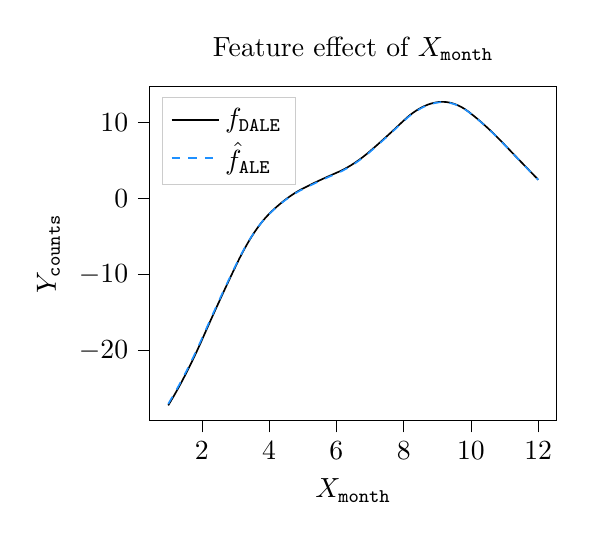
\begin{tikzpicture}

\definecolor{darkgray176}{RGB}{176,176,176}
\definecolor{dodgerblue}{RGB}{30,144,255}
\definecolor{lightgray204}{RGB}{204,204,204}

\begin{axis}[
legend cell align={left},
legend style={
  fill opacity=0.8,
  draw opacity=1,
  text opacity=1,
  at={(0.03,0.97)},
  anchor=north west,
  draw=lightgray204
},
tick align=outside,
tick pos=left,
title={Feature effect of \(\displaystyle X_{\mathtt{month}}\)},
x grid style={darkgray176},
xlabel={\(\displaystyle X_{\mathtt{month}}\)},
xmin=0.45, xmax=12.55,
xtick style={color=black},
y grid style={darkgray176},
ylabel={\(\displaystyle Y_{\mathtt{counts}}\)},
ymin=-29.183798458369, ymax=14.7468616660552,
ytick style={color=black}
]
\addplot [semithick, black]
table {%
1 -27.1869506835938
1.17617619037628 -25.871150970459
1.29729723930359 -24.9201946258545
1.40740740299225 -24.0201549530029
1.51751756668091 -23.0867099761963
1.63863861560822 -22.0221939086914
1.74874877929688 -21.0186061859131
1.85885882377625 -19.9816131591797
1.9689689874649 -18.9112167358398
2.09009003639221 -17.6963996887207
2.32132124900818 -15.3969707489014
2.64064073562622 -12.2988424301147
2.87187194824219 -10.1101322174072
3.1141140460968 -7.87898731231689
3.24624633789062 -6.75733757019043
3.35635638237 -5.88665103912354
3.45545554161072 -5.15343141555786
3.56556558609009 -4.3964409828186
3.67567563056946 -3.69928789138794
3.77477478981018 -3.12166857719421
3.88488483428955 -2.53821158409119
3.99499487876892 -2.01459169387817
4.13813829421997 -1.40747404098511
4.23723745346069 -1.0118283033371
4.34734725952148 -0.59662914276123
4.45745754241943 -0.207057595252991
4.56756734848022 0.156886339187622
4.66666650772095 0.462822675704956
4.7767767906189 0.778071641921997
4.88688707351685 1.06769299507141
4.98598575592041 1.30698728561401
5.21721744537354 1.81831657886505
5.43743753433228 2.28735709190369
5.64664649963379 2.71674489974976
5.86686706542969 3.15148568153381
6.12012004852295 3.64487433433533
6.19719696044922 3.81250214576721
6.30730724334717 4.07315158843994
6.42842864990234 4.38769626617432
6.53853845596313 4.69808197021484
6.64864873886108 5.03215312957764
6.75875854492188 5.3899097442627
6.87987995147705 5.81102657318115
6.98998975753784 6.21852016448975
7.23223209381104 7.15501070022583
7.463463306427 8.071533203125
7.6836838722229 8.96508026123047
7.90390396118164 9.87869548797607
8.09109115600586 10.6491012573242
8.17917919158936 10.9760904312134
8.27827835083008 11.3111982345581
8.38838863372803 11.6416292190552
8.49849891662598 11.9293622970581
8.60860824584961 12.1743965148926
8.70770740509033 12.3600397109985
8.81781768798828 12.5239429473877
8.92792797088623 12.6451482772827
9.03803825378418 12.7230014801025
9.1371374130249 12.7500133514404
9.17016983032227 12.7448768615723
9.24724769592285 12.7297611236572
9.28028011322021 12.7090911865234
9.35735702514648 12.6578493118286
9.40140151977539 12.6091642379761
9.47847843170166 12.5178241729736
9.58858871459961 12.3373823165894
9.69869899749756 12.1052808761597
9.80880928039551 11.8215208053589
9.92992973327637 11.4478168487549
10.1061058044434 10.8241405487061
10.2162160873413 10.4159374237061
10.3263263702393 9.99349880218506
10.4364366531372 9.55682373046875
10.5575571060181 9.06051921844482
10.667667388916 8.59395122528076
10.777777671814 8.11314868927002
10.8988990783691 7.56844854354858
11.7247247695923 3.76278614997864
12 2.50704598426819
};
\addlegendentry{$f_{\mathtt{DALE}}$}
\addplot [semithick, dodgerblue, dashed]
table {%
1 -27.0010604858398
1.18718719482422 -25.586950302124
1.29729723930359 -24.7142314910889
1.40740740299225 -23.809778213501
1.52852857112885 -22.77903175354
1.63863861560822 -21.8079357147217
1.74874877929688 -20.8051052093506
1.86986982822418 -19.666467666626
1.99099099636078 -18.4894695281982
2.2992992401123 -15.4285402297974
2.51951956748962 -13.2975368499756
2.72872877120972 -11.3166017532349
2.94894886016846 -9.27656745910645
3.1141140460968 -7.78738117218018
3.24624633789062 -6.68413352966309
3.35635638237 -5.82812023162842
3.45545554161072 -5.10758543014526
3.56556558609009 -4.36409330368042
3.67567563056946 -3.67981958389282
3.77477478981018 -3.113276720047
3.88488483428955 -2.54152417182922
3.99499487876892 -2.02899026870728
4.13813829421997 -1.43530428409576
4.23723745346069 -1.04830312728882
4.34734725952148 -0.642061471939087
4.45745754241943 -0.260767459869385
4.56756734848022 0.0955789089202881
4.66666650772095 0.395250797271729
4.7767767906189 0.704194068908691
4.88688707351685 0.988189816474915
4.98598575592041 1.22298789024353
5.23923921585083 1.77311503887177
5.4484486579895 2.21300554275513
5.66866874694824 2.66170525550842
5.88888883590698 3.09569883346558
6.10910892486572 3.52712678909302
6.19719696044922 3.71933627128601
6.30730724334717 3.9817156791687
6.42842864990234 4.29802989959717
6.53853845596313 4.60990715026855
6.64864873886108 4.9453558921814
6.75875854492188 5.30437612533569
6.87987995147705 5.72675085067749
6.98998975753784 6.13526916503906
7.24324321746826 7.11681127548218
7.463463306427 7.99168014526367
7.6836838722229 8.8862886428833
7.90390396118164 9.80063629150391
8.09109115600586 10.5716905593872
8.17917919158936 10.899432182312
8.2892894744873 11.2697401046753
8.38838863372803 11.5681610107422
8.49849891662598 11.8583631515503
8.60860824584961 12.106406211853
8.70770740509033 12.2951984405518
8.81781768798828 12.463134765625
8.92792797088623 12.5889139175415
9.03803825378418 12.6718053817749
9.1371374130249 12.702956199646
9.17016983032227 12.6990699768066
9.24724769592285 12.6868410110474
9.28028011322021 12.6672773361206
9.35735702514648 12.6185913085938
9.40140151977539 12.5711889266968
9.47847843170166 12.4820346832275
9.58858871459961 12.3042573928833
9.69869899749756 12.0743465423584
9.80880928039551 11.7923011779785
9.92992973327637 11.4199190139771
10.1061058044434 10.7974834442139
10.2162160873413 10.3899793624878
10.3263263702393 9.96817970275879
10.4364366531372 9.53208541870117
10.5575571060181 9.03635120391846
10.667667388916 8.57023906707764
10.777777671814 8.08983135223389
10.8988990783691 7.54549980163574
11.7027025222778 3.84338307380676
12 2.48848509788513
};
\addlegendentry{$\hat{f}_{\mathtt{ALE}}$}
\end{axis}

\end{tikzpicture}
}
  \resizebox{.3\columnwidth}{!}{% This file was created with tikzplotlib v0.10.1.
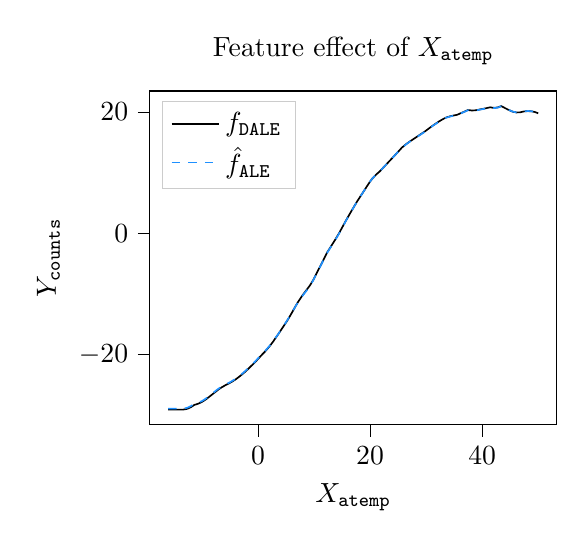
\begin{tikzpicture}

\definecolor{darkgray176}{RGB}{176,176,176}
\definecolor{dodgerblue}{RGB}{30,144,255}
\definecolor{lightgray204}{RGB}{204,204,204}

\begin{axis}[
legend cell align={left},
legend style={
  fill opacity=0.8,
  draw opacity=1,
  text opacity=1,
  at={(0.03,0.97)},
  anchor=north west,
  draw=lightgray204
},
tick align=outside,
tick pos=left,
title={Feature effect of \(\displaystyle X_{\mathtt{atemp}}\)},
x grid style={darkgray176},
xlabel={\(\displaystyle X_{\mathtt{atemp}}\)},
xmin=-19.3, xmax=53.3,
xtick style={color=black},
y grid style={darkgray176},
ylabel={\(\displaystyle Y_{\mathtt{counts}}\)},
ymin=-31.6301535780892, ymax=23.4795271752803,
ytick style={color=black}
]
\addplot [semithick, black]
table {%
-16 -29.1201610565186
-14.5465469360352 -29.1236610412598
-13.3573570251465 -29.1187324523926
-12.6306304931641 -28.9887657165527
-11.9699697494507 -28.7167987823486
-11.3753757476807 -28.351110458374
-10.5825824737549 -28.10817527771
-9.9219217300415 -27.8089466094971
-9.26126098632812 -27.4157428741455
-8.13813781738281 -26.5979690551758
-6.94894886016846 -25.7284774780273
-6.55255270004272 -25.4859237670898
-5.89189195632935 -25.1317119598389
-4.70270252227783 -24.557861328125
-3.90990996360779 -24.0795192718506
-3.11711716651917 -23.5240688323975
-2.52252244949341 -23.0663394927979
-1.86186182498932 -22.5092353820801
-0.540540456771851 -21.3122959136963
0.120120167732239 -20.6509094238281
0.714714765548706 -20.0558643341064
1.30930936336517 -19.4900760650635
2.03603601455688 -18.7049884796143
2.63063073158264 -17.9895362854004
3.8858859539032 -16.3134365081787
5.27327346801758 -14.3682708740234
6 -13.2194204330444
6.85885906219482 -11.8082704544067
7.25525522232056 -11.203857421875
7.91591596603394 -10.3020009994507
9.30330371856689 -8.58228397369385
9.83183193206787 -7.77181529998779
10.9549551010132 -5.72904586791992
12.342342376709 -3.19349336624146
12.5405406951904 -2.89349699020386
13.7957954406738 -1.05008816719055
14.4564561843872 -0.0256915092468262
15.6456460952759 2.00035262107849
16.5705699920654 3.49347949028015
17.6936931610107 5.24578619003296
19.9399394989014 8.44653511047363
20.4024028778076 9.01027202606201
21.0630626678467 9.66129207611084
21.7237243652344 10.1941547393799
24.8948955535889 13.3221054077148
25.687686920166 14.134651184082
26.4804801940918 14.7308025360107
27.1411418914795 15.1683645248413
29.8498497009277 16.8362903594971
30.7087078094482 17.4392356872559
31.3693695068359 17.8697376251221
32.3603591918945 18.484224319458
33.087085723877 18.8724536895752
33.5495491027832 19.0880432128906
34.4084091186523 19.3274822235107
35.0690689086914 19.4596900939941
35.5315322875977 19.543493270874
36.9849853515625 20.1296157836914
37.4474487304688 20.3274917602539
37.6456451416016 20.3095550537109
38.1741752624512 20.2521419525146
38.8348350524902 20.287296295166
39.8258247375488 20.4710922241211
40.6186180114746 20.6114158630371
41.345344543457 20.7675323486328
41.4114112854004 20.7821464538574
41.8078079223633 20.7240734100342
42.1381378173828 20.6876392364502
42.7987976074219 20.7667903900146
43.3933944702148 20.9745426177979
43.657657623291 20.8512020111084
44.714714050293 20.3551597595215
45.4414405822754 20.057201385498
46.1021003723145 19.9324207305908
46.7627639770508 19.9523639678955
47.4894905090332 20.1014881134033
48.1501502990723 20.1500225067139
48.8108100891113 20.1130447387695
49.4054069519043 20.0048065185547
50 19.7889881134033
};
\addlegendentry{$f_{\mathtt{DALE}}$}
\addplot [semithick, dodgerblue, dashed]
table {%
-16 -28.9542388916016
-14.5465469360352 -28.9578762054443
-13.3573570251465 -28.9526977539062
-12.6306304931641 -28.8202018737793
-11.9699697494507 -28.5466842651367
-11.3753757476807 -28.1803741455078
-10.6486482620239 -27.9906787872314
-9.98798751831055 -27.7104911804199
-9.26126098632812 -27.2779521942139
-8.00600624084473 -26.3645648956299
-7.2132134437561 -25.7814712524414
-6.55255270004272 -25.3670864105225
-5.89189195632935 -25.0190086364746
-4.76876878738403 -24.4896812438965
-3.90990996360779 -23.9704494476318
-3.05105113983154 -23.364631652832
-2.52252244949341 -22.9567375183105
-1.86186182498932 -22.4021339416504
-0.606606602668762 -21.2720623016357
0.120120167732239 -20.5483741760254
0.648648619651794 -20.0188083648682
1.30930936336517 -19.4072608947754
1.96996998786926 -18.7101631164551
2.69669675827026 -17.8467922210693
3.55555558204651 -16.7303333282471
4.21621608734131 -15.8174858093262
5.53753757476807 -13.9267387390137
6 -13.1932601928711
6.66066074371338 -12.1299390792847
7.32132148742676 -11.1632461547852
7.91591596603394 -10.3738870620728
8.97297286987305 -9.1130838394165
9.10510540008545 -8.9506664276123
9.83183193206787 -7.83912706375122
11.2852849960327 -5.17018270492554
12.408408164978 -3.13905572891235
13.5975971221924 -1.41476833820343
14.3243246078491 -0.306623458862305
14.6546545028687 0.264089107513428
15.6456460952759 1.96240651607513
16.5705699920654 3.46715188026428
17.6936931610107 5.24065256118774
19.8738746643066 8.35614967346191
20.4024028778076 9.0117301940918
21.0630626678467 9.66457653045654
21.7237243652344 10.1938533782959
25.4894886016846 13.9263477325439
25.6216220855713 14.053521156311
26.4804801940918 14.7064094543457
27.1411418914795 15.1473188400269
29.057056427002 16.3006134033203
29.6516513824463 16.6701507568359
30.6426429748535 17.3715686798096
31.2372379302979 17.7557601928711
32.4924926757812 18.524055480957
33.087085723877 18.8392581939697
33.5495491027832 19.0558605194092
34.4084091186523 19.2951412200928
35.0690689086914 19.4283008575439
35.5315322875977 19.5130195617676
36.9849853515625 20.0959377288818
37.4474487304688 20.291877746582
37.6456451416016 20.2738914489746
38.1741752624512 20.216480255127
38.8348350524902 20.2516288757324
39.8258247375488 20.4354114532471
40.6186180114746 20.5759296417236
41.2792778015137 20.7178859710693
41.4114112854004 20.7472190856934
41.8078079223633 20.6907978057861
42.1381378173828 20.6556282043457
42.7987976074219 20.7358493804932
43.3933944702148 20.9432563781738
43.657657623291 20.8323345184326
45.375373840332 20.0885391235352
46.0360374450684 19.9492740631104
46.6966972351074 19.9548187255859
47.5555572509766 20.1251811981201
48.1501502990723 20.1673374176025
48.8108100891113 20.1304454803467
49.4054069519043 20.0222206115723
50 19.8063983917236
};
\addlegendentry{$\hat{f}_{\mathtt{ALE}}$}
\end{axis}

\end{tikzpicture}
}
  \resizebox{.3\columnwidth}{!}{% This file was created with tikzplotlib v0.10.1.
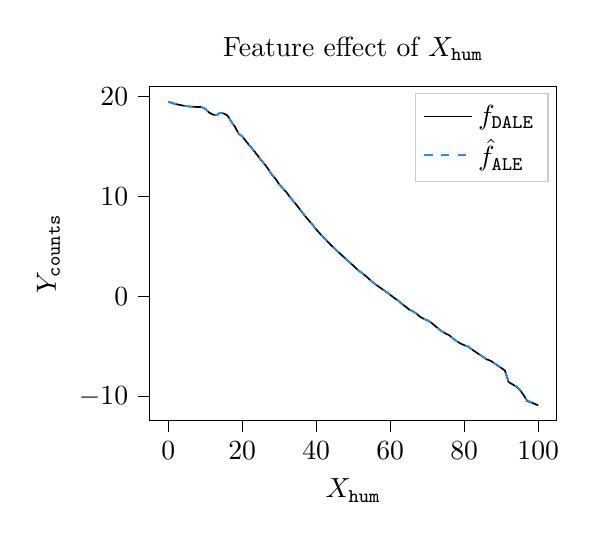
\begin{tikzpicture}

\definecolor{darkgray176}{RGB}{176,176,176}
\definecolor{dodgerblue}{RGB}{30,144,255}
\definecolor{lightgray204}{RGB}{204,204,204}

\begin{axis}[
legend cell align={left},
legend style={fill opacity=0.8, draw opacity=1, text opacity=1, draw=lightgray204},
tick align=outside,
tick pos=left,
title={Feature effect of \(\displaystyle X_{\mathtt{hum}}\)},
x grid style={darkgray176},
xlabel={\(\displaystyle X_{\mathtt{hum}}\)},
xmin=-5, xmax=105,
xtick style={color=black},
y grid style={darkgray176},
ylabel={\(\displaystyle Y_{\mathtt{counts}}\)},
ymin=-12.4017583163331, ymax=20.9680093156312,
ytick style={color=black}
]
\addplot [semithick, black]
table {%
0 19.445671081543
1.80180180072784 19.2508811950684
2.8028028011322 19.1621017456055
3.80380392074585 19.0876598358154
4.80480480194092 19.0275573730469
5.80580568313599 18.9817924499512
6.80680704116821 18.9503650665283
7.80780792236328 18.933277130127
8.80880928039551 18.9305267333984
9.00900936126709 18.9289054870605
10.010009765625 18.7470264434814
11.0110111236572 18.3885173797607
12.0120124816895 18.1801509857178
13.0130128860474 18.1236801147461
14.0140142440796 18.3442001342773
15.0150146484375 18.2827415466309
16.0160160064697 18.0843563079834
17.1171169281006 17.4235782623291
18.0180187225342 16.9714221954346
19.0190181732178 16.268253326416
20.02001953125 15.9827404022217
21.2212219238281 15.4168157577515
23.2232227325439 14.5354175567627
24.4244251251221 13.9460258483887
25.325325012207 13.5335330963135
26.2262268066406 13.1304426193237
27.027027130127 12.738260269165
28.0280284881592 12.1465797424316
29.0290298461914 11.7472257614136
30.030029296875 11.1805286407471
31.9319324493408 10.4186792373657
32.1321334838867 10.3230867385864
33.033031463623 9.86366176605225
34.1341323852539 9.40140438079834
36.9369354248047 8.0537805557251
37.4374389648438 7.83730363845825
39.2392387390137 7.05814123153687
40.1401405334473 6.63687181472778
41.5415420532227 6.06709289550781
42.5425415039062 5.68619441986084
43.3433418273926 5.3793511390686
44.1441459655762 5.07060098648071
45.1451454162598 4.7441782951355
46.2462463378906 4.34106254577637
50.1501502990723 3.03945064544678
51.1511497497559 2.67909049987793
52.352352142334 2.33571791648865
53.1531524658203 2.11605978012085
54.5545539855957 1.6564826965332
55.1551551818848 1.46061563491821
56.6566581726074 1.04154002666473
58.0580596923828 0.674215078353882
59.4594612121582 0.312742352485657
60.4604606628418 0.0281145572662354
61.1611595153809 -0.170746326446533
62.0620613098145 -0.390427708625793
63.1631622314453 -0.749048829078674
64.1641616821289 -1.0204029083252
65.0650634765625 -1.29337751865387
66.1661682128906 -1.49768507480621
67.0670700073242 -1.71112847328186
68.0680694580078 -2.03258061408997
69.0690689086914 -2.23863196372986
70.070068359375 -2.38389420509338
71.0710678100586 -2.61734461784363
73.3733749389648 -3.33057689666748
74.1741714477539 -3.53978538513184
75.175178527832 -3.74607062339783
75.9759750366211 -3.88061666488647
76.3763732910156 -4.00896739959717
77.1771774291992 -4.26187658309937
78.2782745361328 -4.54429483413696
79.0790786743164 -4.72437953948975
80.1801834106445 -4.89549112319946
80.9809799194336 -4.98908805847168
81.3813781738281 -5.09695863723755
82.8828811645508 -5.50094985961914
83.5835800170898 -5.67414093017578
84.584587097168 -5.90682792663574
85.185188293457 -6.05287551879883
85.9859848022461 -6.28149127960205
86.4864883422852 -6.34115266799927
87.0870895385742 -6.42070388793945
88.6886901855469 -6.81395483016968
90.9909896850586 -7.4021258354187
91.2912902832031 -7.73944664001465
91.9919891357422 -8.54510974884033
92.1921920776367 -8.59602737426758
94.0940933227539 -9.01366710662842
94.9949951171875 -9.32887077331543
95.9959945678711 -9.81900787353516
96.9969940185547 -10.4498987197876
97.7977981567383 -10.5560169219971
98.7987976074219 -10.6977682113647
99.7997970581055 -10.85329246521
100 -10.8849506378174
};
\addlegendentry{$f_{\mathtt{DALE}}$}
\addplot [semithick, dodgerblue, dashed]
table {%
0 19.4512023925781
1.80180180072784 19.2567539215088
2.8028028011322 19.1681327819824
3.80380392074585 19.093822479248
4.80480480194092 19.0338249206543
5.80580568313599 18.9881401062012
6.80680704116821 18.9567699432373
7.80780792236328 18.9397106170654
8.80880928039551 18.9369659423828
9.00900936126709 18.9353446960449
10.010009765625 18.753490447998
11.0110111236572 18.3950309753418
12.0120124816895 18.1866893768311
13.0130128860474 18.1302185058594
14.0140142440796 18.3507404327393
15.0150146484375 18.289701461792
16.0160160064697 18.0913181304932
17.1171169281006 17.4305477142334
18.0180187225342 16.9784984588623
19.0190181732178 16.2804527282715
20.02001953125 15.9955158233643
21.2212219238281 15.4311323165894
23.1231231689453 14.5908050537109
24.3243236541748 13.9988222122192
25.325325012207 13.5421257019043
26.1261253356934 13.187403678894
27.027027130127 12.7418575286865
28.0280284881592 12.1519727706909
29.0290298461914 11.7499494552612
30.030029296875 11.182975769043
32.0320320129395 10.3707160949707
33.033031463623 9.85312747955322
34.1341323852539 9.38883113861084
36.6366348266602 8.18614196777344
37.1371383666992 7.95634317398071
39.0390396118164 7.15220594406128
40.1401405334473 6.63696813583374
41.4414405822754 6.10159015655518
42.4424438476562 5.71701908111572
43.3433418273926 5.37234306335449
44.1441459655762 5.06235647201538
45.1451454162598 4.73639726638794
46.2462463378906 4.33528661727905
50.050048828125 3.06395077705383
51.1511497497559 2.66571760177612
52.2522506713867 2.34696483612061
53.1531524658203 2.10619187355042
54.5545539855957 1.64742040634155
55.1551551818848 1.4514753818512
56.5565567016602 1.06200659275055
58.1581573486328 0.648456811904907
59.4594612121582 0.313627243041992
60.4604606628418 0.0284990072250366
61.1611595153809 -0.170641422271729
62.0620613098145 -0.391844630241394
63.0630645751953 -0.725825071334839
64.2642669677734 -1.05191004276276
65.0650634765625 -1.28894066810608
66.1661682128906 -1.49367189407349
67.0670700073242 -1.70696103572845
68.0680694580078 -2.03458189964294
69.0690689086914 -2.24001359939575
70.070068359375 -2.38448262214661
71.0710678100586 -2.62038135528564
73.2732696533203 -3.31713366508484
74.1741714477539 -3.55359435081482
75.175178527832 -3.7575466632843
75.9759750366211 -3.88404536247253
76.2762756347656 -3.97914242744446
77.1771774291992 -4.2657265663147
78.2782745361328 -4.54978799819946
79.1791763305664 -4.74476099014282
80.1801834106445 -4.89946508407593
80.9809799194336 -4.99041557312012
81.3813781738281 -5.09758758544922
82.9829864501953 -5.52745628356934
84.2842864990234 -5.83696460723877
85.185188293457 -6.04725694656372
85.9859848022461 -6.27391958236694
86.4864883422852 -6.33382940292358
87.0870895385742 -6.41337013244629
88.6886901855469 -6.80084180831909
90.9909896850586 -7.36907291412354
91.2912902832031 -7.70228242874146
91.9919891357422 -8.49856758117676
92.1921920776367 -8.5493803024292
94.0940933227539 -8.96699905395508
94.9949951171875 -9.28218460083008
95.9959945678711 -9.77230548858643
96.9969940185547 -10.4031848907471
97.7977981567383 -10.509295463562
98.5986022949219 -10.6244306564331
99.5996017456055 -10.7833385467529
100 -10.8497257232666
};
\addlegendentry{$\hat{f}_{\mathtt{ALE}}$}
\end{axis}

\end{tikzpicture}
}
  \caption{Bike-Sharing Dataset. DALE and ALE feature effect plots with \(K=200\) for:
    \(X_{\texttt{month}}\), \(X_{\mathtt{atemp}}\),\(X_{\mathtt{hum}}\).}
  \label{fig:bike-sharing-comparison}
\end{figure}


\begin{figure}[h]
  \centering
    \resizebox{.3\columnwidth}{!}{% This file was created with tikzplotlib v0.10.1.
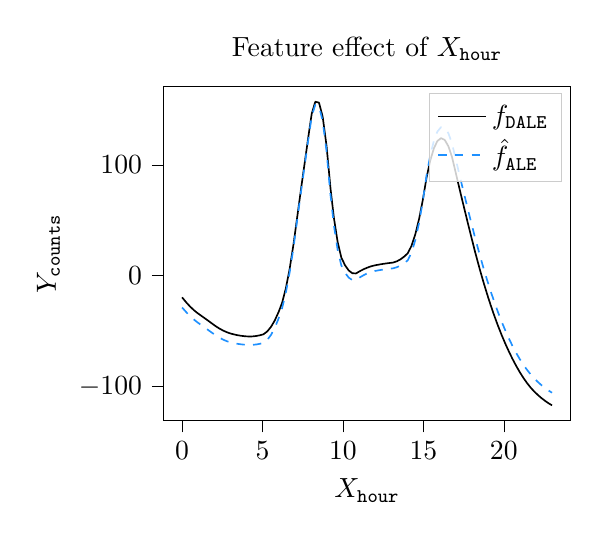
\begin{tikzpicture}

\definecolor{darkgray176}{RGB}{176,176,176}
\definecolor{dodgerblue}{RGB}{30,144,255}
\definecolor{lightgray204}{RGB}{204,204,204}

\begin{axis}[
legend cell align={left},
legend style={fill opacity=0.8, draw opacity=1, text opacity=1, draw=lightgray204},
tick align=outside,
tick pos=left,
title={Feature effect of \(\displaystyle X_{\mathtt{hour}}\)},
x grid style={darkgray176},
xlabel={\(\displaystyle X_{\mathtt{hour}}\)},
xmin=-1.15, xmax=24.15,
xtick style={color=black},
y grid style={darkgray176},
ylabel={\(\displaystyle Y_{\mathtt{counts}}\)},
ymin=-130.55351264475, ymax=170.472616656964,
ytick style={color=black}
]
\addplot [semithick, black]
table {%
0 -19.5050849914551
0.276276350021362 -24.3441772460938
0.506506443023682 -27.9236030578613
0.73673677444458 -31.0645523071289
0.943943977355957 -33.5316467285156
1.54254257678986 -39.7169952392578
2.00300312042236 -44.5988159179688
2.11811804771423 -45.7644081115723
2.32532525062561 -47.663459777832
2.55555558204651 -49.4630393981934
2.78578567504883 -50.9483070373535
2.99299287796021 -52.0300178527832
3.24624633789062 -52.9924545288086
3.47647643089294 -53.6967239379883
3.68368363380432 -54.1934471130371
3.91391396522522 -54.5767364501953
4.14414405822754 -54.7889671325684
4.37437438964844 -54.7139015197754
4.60460472106934 -54.3515357971191
4.83483505249023 -53.7018775939941
5.04204225540161 -52.8642959594727
5.06506490707397 -52.7370185852051
5.29529523849487 -50.2154121398926
5.52552556991577 -46.1370544433594
5.75575590133667 -40.5019493103027
6.00900888442993 -32.4394378662109
6.21621608734131 -24.4946517944336
6.44644641876221 -11.6443128585815
6.67667675018311 5.24092245101929
6.92992973327637 28.6440601348877
7.43643665313721 82.6207962036133
7.89689683914185 130.067947387695
8.05805778503418 145.936157226562
8.26526546478271 156.092514038086
8.28828811645508 156.789611816406
8.49549579620361 156.161087036133
8.51851844787598 155.647872924805
8.72572612762451 144.234481811523
8.74874877929688 142.510955810547
8.97897911071777 117.378860473633
9.23223209381104 78.1012954711914
9.43943977355957 52.0760345458984
9.66967010498047 30.5269412994385
9.89989948272705 16.3793964385986
10.1301298141479 9.40791988372803
10.3603601455688 4.70836496353149
10.5675678253174 2.42953133583069
10.5905904769897 2.28073143959045
10.7977981567383 2.04458355903625
10.8208208084106 2.12501859664917
11.0740737915039 4.29217100143433
11.3043041229248 5.98237943649292
11.5345344543457 7.39637041091919
11.7417421340942 8.44379425048828
11.9719715118408 9.33294486999512
12.2482481002808 10.0710592269897
12.4784784317017 10.624490737915
12.7087087631226 11.1187515258789
12.9159154891968 11.5147294998169
13.1001005172729 11.8276166915894
13.1231231689453 11.9058475494385
13.3303298950195 12.875524520874
13.3763761520386 13.199444770813
13.5835838317871 14.8272914886475
13.813814163208 17.3185062408447
14.0210208892822 20.1412181854248
14.0670671463013 21.3190975189209
14.2512512207031 26.5641231536865
14.2972974777222 28.4294090270996
14.5045042037964 37.6234588623047
14.7347345352173 51.2384872436523
14.9649648666382 68.2768707275391
15.1951951980591 88.2222595214844
15.42542552948 103.759735107422
15.6556558609009 114.889282226562
15.8628625869751 121.212203979492
15.8858861923218 121.610908508301
16.0930938720703 123.970664978027
16.1161155700684 123.936637878418
16.3233242034912 122.487854003906
16.3693695068359 121.442276000977
16.5535526275635 116.769096374512
16.6226234436035 113.865631103516
16.7837829589844 106.814399719238
16.8758754730225 101.206695556641
17.3363361358643 72.9654541015625
17.7967967987061 45.5679664611816
18.2112121582031 21.7020950317383
18.5105113983154 5.64360857009888
18.7407398223877 -5.97945785522461
18.9709701538086 -16.9456024169922
19.1781787872314 -26.2628364562988
19.4084091186523 -35.9988479614258
19.6386394500732 -45.0910110473633
19.8688697814941 -53.5393295288086
20.0990982055664 -61.3896484375
20.3293285369873 -68.7146987915039
20.5365371704102 -74.8665542602539
20.7667675018311 -81.1935348510742
20.996997833252 -86.995246887207
21.2042045593262 -91.7762222290039
21.4344348907471 -96.5489959716797
21.664665222168 -100.770584106445
21.8948955535889 -104.44100189209
22.1481475830078 -107.900184631348
22.3553562164307 -110.46851348877
22.5855846405029 -113.02222442627
22.8158149719238 -115.269233703613
23 -116.870506286621
};
\addlegendentry{$f_{\mathtt{DALE}}$}
\addplot [semithick, dodgerblue, dashed]
table {%
0 -28.6461296081543
0.299299240112305 -33.4844398498535
0.506506443023682 -36.5122833251953
0.73673677444458 -39.5242080688477
0.966966986656189 -42.1757049560547
1.74974977970123 -50.2825317382812
2.11811804771423 -54.0799827575684
2.32532525062561 -55.9247512817383
2.55555558204651 -57.6483955383301
2.78578567504883 -59.0419044494629
2.99299287796021 -60.0281982421875
3.24624633789062 -60.8593711853027
3.47647643089294 -61.46630859375
3.68368363380432 -61.8931121826172
3.91391396522522 -62.2204475402832
4.14414405822754 -62.3986968994141
4.37437438964844 -62.3219032287598
4.60460472106934 -61.990062713623
4.83483505249023 -61.4031791687012
5.04204225540161 -60.6504898071289
5.06506490707397 -60.5277214050293
5.29529523849487 -57.8714256286621
5.52552556991577 -53.4342956542969
5.75575590133667 -47.2163352966309
6.00900888442993 -38.2443809509277
6.21621608734131 -29.381742477417
6.44644641876221 -15.6827802658081
6.69969987869263 4.01029825210571
6.92992973327637 25.8215217590332
7.39039039611816 75.5200271606445
7.85085105895996 123.192329406738
8.05805778503418 143.596130371094
8.26526546478271 153.462203979492
8.28828811645508 154.119873046875
8.49549579620361 153.021850585938
8.51851844787598 152.449096679688
8.72572612762451 140.386978149414
8.74874877929688 138.58381652832
8.97897911071777 112.524017333984
9.20920944213867 75.0672760009766
9.43943977355957 45.3751182556152
9.66967010498047 23.4475517272949
9.89989948272705 9.28457546234131
10.1301298141479 2.64411807060242
10.3603601455688 -1.73881900310516
10.5675678253174 -3.74506211280823
10.5905904769897 -3.86423587799072
10.7977981567383 -3.84074091911316
10.8208208084106 -3.73213291168213
11.0740737915039 -1.27214574813843
11.3043041229248 0.624772906303406
11.5115118026733 2.059002161026
11.7417421340942 3.31951761245728
11.9719715118408 4.24510145187378
12.2482481002808 4.96000051498413
12.4784784317017 5.49322175979614
12.7087087631226 5.96644258499146
12.9159154891968 6.34280109405518
13.1001005172729 6.63770151138306
13.1231231689453 6.70726346969604
13.3303298950195 7.55532884597778
13.3763761520386 7.83442735671997
13.5835838317871 9.23264122009277
13.813814163208 11.3566951751709
14.0210208892822 13.7536668777466
14.0440444946289 14.2715625762939
14.2512512207031 20.38014793396
14.2972974777222 22.4057006835938
14.5045042037964 32.4857139587402
14.7347345352173 47.7849960327148
14.9649648666382 67.2124176025391
15.1951951980591 90.178352355957
15.42542552948 108.329772949219
15.6556558609009 121.666687011719
15.8628625869751 129.635528564453
15.9089088439941 130.593536376953
16.0930938720703 133.829193115234
16.1161155700684 133.91423034668
16.3233242034912 133.447540283203
16.3463459014893 133.071701049805
16.5535526275635 128.498184204102
16.5995998382568 126.696998596191
16.7837829589844 118.981163024902
16.8758754730225 113.421195983887
17.3363361358643 85.3754196166992
17.7967967987061 58.1768074035645
18.2112121582031 34.4831466674805
18.5335330963135 17.2674236297607
18.7407398223877 6.80826711654663
18.9709701538086 -4.24147033691406
19.2012004852295 -14.6806631088257
19.4084091186523 -23.5517692565918
19.6386394500732 -32.8170890808105
19.8688697814941 -41.4646186828613
20.0990982055664 -49.5049858093262
20.3063068389893 -56.2461433410645
20.5365371704102 -63.1648941040039
20.7667675018311 -69.4933547973633
20.9739742279053 -74.6995239257812
21.2272281646729 -80.4064331054688
21.4344348907471 -84.651123046875
21.664665222168 -88.8804550170898
21.8948955535889 -92.6121520996094
22.1481475830078 -96.1844940185547
22.3553562164307 -98.8407440185547
22.5855846405029 -101.486793518066
22.8158149719238 -103.820686340332
23 -105.487968444824
};
\addlegendentry{$\hat{f}_{\mathtt{ALE}}$}
\end{axis}

\end{tikzpicture}
}
    \resizebox{.3\columnwidth}{!}{% This file was created with tikzplotlib v0.10.1.
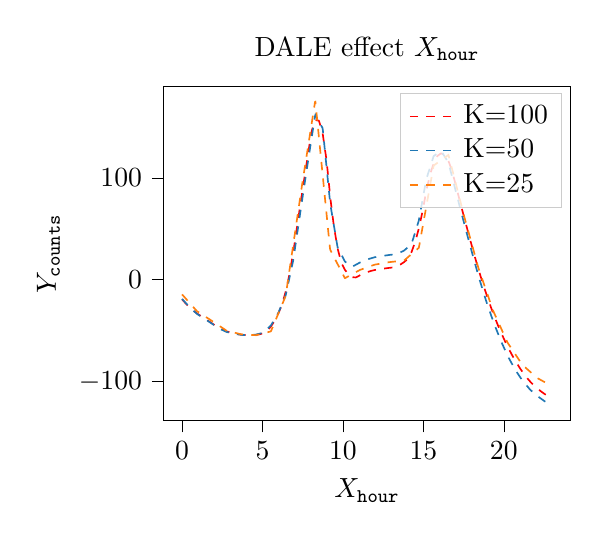
\begin{tikzpicture}

\definecolor{darkgray176}{RGB}{176,176,176}
\definecolor{darkorange25512714}{RGB}{255,127,14}
\definecolor{lightgray204}{RGB}{204,204,204}
\definecolor{steelblue31119180}{RGB}{31,119,180}

\begin{axis}[
legend cell align={left},
legend style={fill opacity=0.8, draw opacity=1, text opacity=1, draw=lightgray204},
tick align=outside,
tick pos=left,
title={DALE effect \(\displaystyle X_{\mathtt{hour}}\)},
x grid style={darkgray176},
xlabel={\(\displaystyle X_{\mathtt{hour}}\)},
xmin=-1.15, xmax=24.15,
xtick style={color=black},
y grid style={darkgray176},
ylabel={\(\displaystyle Y_{\mathtt{counts}}\)},
ymin=-138.606064986267, ymax=189.589636529361,
ytick style={color=black}
]
\addplot [semithick, red, dashed]
table {%
0 -19.5050849914551
0.276276350021362 -24.3441772460938
0.506506443023682 -27.9236030578613
0.73673677444458 -31.0645523071289
0.943943977355957 -33.5316467285156
1.54254257678986 -39.7169952392578
2.00300312042236 -44.5988159179688
2.11811804771423 -45.7644081115723
2.32532525062561 -47.663459777832
2.55555558204651 -49.4630393981934
2.78578567504883 -50.9483070373535
2.99299287796021 -52.0300178527832
3.24624633789062 -52.9924545288086
3.47647643089294 -53.6967239379883
3.68368363380432 -54.1934471130371
3.91391396522522 -54.5767364501953
4.14414405822754 -54.7889671325684
4.37437438964844 -54.7139015197754
4.60460472106934 -54.3515357971191
4.83483505249023 -53.7018775939941
5.04204225540161 -52.8642959594727
5.06506490707397 -52.7370185852051
5.29529523849487 -50.2154121398926
5.52552556991577 -46.1370544433594
5.75575590133667 -40.5019493103027
6.00900888442993 -32.4394378662109
6.21621608734131 -24.4946517944336
6.44644641876221 -11.6443128585815
6.67667675018311 5.24092245101929
6.92992973327637 28.6440601348877
7.43643665313721 82.6207962036133
7.89689683914185 130.067947387695
8.05805778503418 145.936157226562
8.26526546478271 156.092514038086
8.28828811645508 156.789611816406
8.49549579620361 156.161087036133
8.51851844787598 155.647872924805
8.72572612762451 144.234481811523
8.74874877929688 142.510955810547
8.97897911071777 117.378860473633
9.23223209381104 78.1012954711914
9.43943977355957 52.0760345458984
9.66967010498047 30.5269412994385
9.89989948272705 16.3793964385986
10.1301298141479 9.40791988372803
10.3603601455688 4.70836496353149
10.5675678253174 2.42953133583069
10.5905904769897 2.28073143959045
10.7977981567383 2.04458355903625
10.8208208084106 2.12501859664917
11.0740737915039 4.29217100143433
11.3043041229248 5.98237943649292
11.5345344543457 7.39637041091919
11.7417421340942 8.44379425048828
11.9719715118408 9.33294486999512
12.2482481002808 10.0710592269897
12.4784784317017 10.624490737915
12.7087087631226 11.1187515258789
12.9159154891968 11.5147294998169
13.1001005172729 11.8276166915894
13.1231231689453 11.9058475494385
13.3303298950195 12.875524520874
13.3763761520386 13.199444770813
13.5835838317871 14.8272914886475
13.813814163208 17.3185062408447
14.0210208892822 20.1412181854248
14.0670671463013 21.3190975189209
14.2512512207031 26.5641231536865
14.2972974777222 28.4294090270996
14.5045042037964 37.6234588623047
14.7347345352173 51.2384872436523
14.9649648666382 68.2768707275391
15.1951951980591 88.2222595214844
15.42542552948 103.759735107422
15.6556558609009 114.889282226562
15.8628625869751 121.212203979492
15.8858861923218 121.610908508301
16.0930938720703 123.970664978027
16.1161155700684 123.936637878418
16.3233242034912 122.487854003906
16.3693695068359 121.442276000977
16.5535526275635 116.769096374512
16.6226234436035 113.865631103516
16.7837829589844 106.814399719238
16.8758754730225 101.206695556641
17.3363361358643 72.9654541015625
17.7967967987061 45.5679664611816
18.2112121582031 21.7020950317383
18.5105113983154 5.64360857009888
18.7407398223877 -5.97945785522461
18.9709701538086 -16.9456024169922
19.1781787872314 -26.2628364562988
19.4084091186523 -35.9988479614258
19.6386394500732 -45.0910110473633
19.8688697814941 -53.5393295288086
20.0990982055664 -61.3896484375
20.3293285369873 -68.7146987915039
20.5365371704102 -74.8665542602539
20.7667675018311 -81.1935348510742
20.996997833252 -86.995246887207
21.2042045593262 -91.7762222290039
21.4344348907471 -96.5489959716797
21.664665222168 -100.770584106445
21.8948955535889 -104.44100189209
22.1481475830078 -107.900184631348
22.3553562164307 -110.46851348877
22.5855846405029 -113.02222442627
22.8158149719238 -115.269233703613
23 -116.870506286621
};
\addlegendentry{K=100}
\addplot [semithick, steelblue31119180, dashed]
table {%
0 -19.0568523406982
0.483483552932739 -27.5899829864502
0.943943977355957 -33.9586143493652
1.65765762329102 -41.3208885192871
2.11811804771423 -46.2027359008789
2.30230236053467 -48.1648330688477
2.76276278495789 -51.5102844238281
3.2232232093811 -53.2904281616211
3.68368363380432 -54.3948593139648
4.12112092971802 -54.8079147338867
4.14414405822754 -54.8193206787109
4.60460472106934 -54.0945930480957
5.04204225540161 -52.3263702392578
5.06506490707397 -52.1762809753418
5.52552556991577 -45.0688095092773
5.98598575592041 -32.7721710205078
6.44644641876221 -15.1332197189331
6.906907081604 18.6453113555908
7.5515513420105 87.5196990966797
8.01201248168945 134.966445922852
8.26526546478271 160.561309814453
8.28828811645508 161.809616088867
8.72572612762451 149.098709106445
8.74874877929688 147.291305541992
9.20920944213867 74.5869293212891
9.66967010498047 31.4887447357178
10.1301298141479 17.5457916259766
10.5675678253174 12.734920501709
10.5905904769897 12.6905250549316
11.0510511398315 16.6829795837402
11.5115118026733 19.7547092437744
11.9719715118408 21.9057159423828
12.4554557800293 23.2053813934326
12.8928928375244 24.1664962768555
13.3303298950195 24.9096031188965
13.3533535003662 25.0283260345459
13.7907905578613 28.3794097900391
13.8368368148804 28.9517726898193
14.2512512207031 34.5971946716309
14.2742738723755 35.4409217834473
14.7117118835449 57.6446723937988
14.757758140564 61.3840827941895
15.1721725463867 97.8089218139648
15.2182178497314 100.394157409668
15.6326322555542 120.966339111328
15.6556558609009 121.510360717773
16.0930938720703 126.492065429688
16.1161155700684 126.161819458008
16.5535526275635 115.063018798828
16.5995998382568 112.439018249512
17.2672672271729 71.3320007324219
17.7277278900146 43.8025321960449
18.1881885528564 16.976188659668
18.4644641876221 1.44218516349792
18.9019012451172 -21.0025215148926
19.362361907959 -42.0182228088379
19.8228225708008 -60.4585456848145
20.2602596282959 -75.6445541381836
20.7207202911377 -89.0095443725586
21.1811809539795 -99.7675628662109
21.6416416168213 -108.320869445801
22.1021022796631 -114.716354370117
22.5625629425049 -119.885055541992
23 -123.688079833984
};
\addlegendentry{K=50}
\addplot [semithick, darkorange25512714, dashed]
table {%
0 -14.6316518783569
0.920920848846436 -31.048433303833
1.97997999191284 -41.9419441223145
2.76276278495789 -50.2953834533691
3.68368363380432 -53.854320526123
4.58158159255981 -54.7021713256836
4.60460472106934 -54.7009506225586
5.50250244140625 -51.0714378356934
5.52552556991577 -50.791748046875
6.42342329025269 -16.8359642028809
6.44644641876221 -15.5138454437256
7.45945930480957 93.0636596679688
8.26526546478271 174.501815795898
8.28828811645508 174.671646118164
9.18618583679199 31.7446269989014
9.20920944213867 29.2628974914551
10.1071071624756 1.68466913700104
10.1301298141479 1.37699365615845
11.0510511398315 9.37294101715088
11.9719715118408 14.6067152023315
12.8928928375244 17.1037063598633
13.7907905578613 18.6290340423584
13.813814163208 18.8328590393066
14.7117118835449 31.0646076202393
14.7347345352173 32.4726219177246
15.6326322555542 111.393112182617
15.6556558609009 112.218955993652
16.5535526275635 122.44457244873
16.5765762329102 121.48802947998
17.5665664672852 60.373119354248
18.4184188842773 11.5534610748291
19.3393402099609 -30.7352237701416
20.2372379302979 -62.1434631347656
20.3753757476807 -65.432746887207
21.1581573486328 -83.8936080932617
21.2962970733643 -85.8475189208984
22.0790786743164 -96.8198623657227
22.3783779144287 -99.4268341064453
23 -104.831130981445
};
\addlegendentry{K=25}
\end{axis}

\end{tikzpicture}
}
    \resizebox{.3\columnwidth}{!}{% This file was created with tikzplotlib v0.10.1.
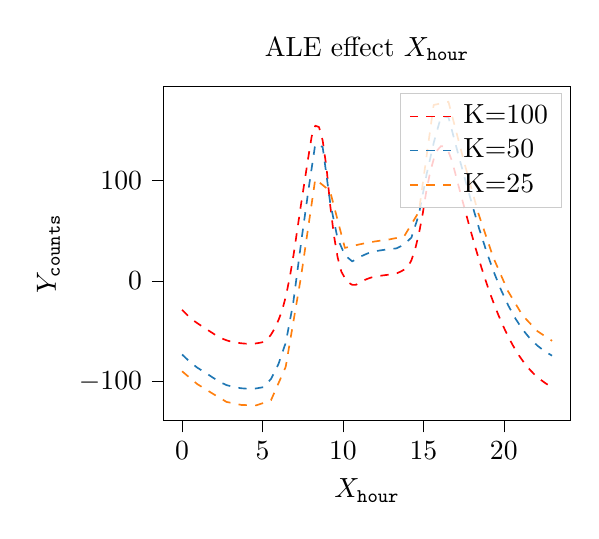
\begin{tikzpicture}

\definecolor{darkgray176}{RGB}{176,176,176}
\definecolor{darkorange25512714}{RGB}{255,127,14}
\definecolor{lightgray204}{RGB}{204,204,204}
\definecolor{steelblue31119180}{RGB}{31,119,180}

\begin{axis}[
legend cell align={left},
legend style={fill opacity=0.8, draw opacity=1, text opacity=1, draw=lightgray204},
tick align=outside,
tick pos=left,
title={ALE effect \(\displaystyle X_{\mathtt{hour}}\)},
x grid style={darkgray176},
xlabel={\(\displaystyle X_{\mathtt{hour}}\)},
xmin=-1.15, xmax=24.15,
xtick style={color=black},
y grid style={darkgray176},
ylabel={\(\displaystyle Y_{\mathtt{counts}}\)},
ymin=-138.606757724745, ymax=192.972018488682,
ytick style={color=black}
]
\addplot [semithick, red, dashed]
table {%
0 -28.6461296081543
0.299299240112305 -33.4844398498535
0.506506443023682 -36.5122833251953
0.73673677444458 -39.5242080688477
0.966966986656189 -42.1757049560547
1.74974977970123 -50.2825317382812
2.11811804771423 -54.0799827575684
2.32532525062561 -55.9247512817383
2.55555558204651 -57.6483955383301
2.78578567504883 -59.0419044494629
2.99299287796021 -60.0281982421875
3.24624633789062 -60.8593711853027
3.47647643089294 -61.46630859375
3.68368363380432 -61.8931121826172
3.91391396522522 -62.2204475402832
4.14414405822754 -62.3986968994141
4.37437438964844 -62.3219032287598
4.60460472106934 -61.990062713623
4.83483505249023 -61.4031791687012
5.04204225540161 -60.6504898071289
5.06506490707397 -60.5277214050293
5.29529523849487 -57.8714256286621
5.52552556991577 -53.4342956542969
5.75575590133667 -47.2163352966309
6.00900888442993 -38.2443809509277
6.21621608734131 -29.381742477417
6.44644641876221 -15.6827802658081
6.69969987869263 4.01029825210571
6.92992973327637 25.8215217590332
7.39039039611816 75.5200271606445
7.85085105895996 123.192329406738
8.05805778503418 143.596130371094
8.26526546478271 153.462203979492
8.28828811645508 154.119873046875
8.49549579620361 153.021850585938
8.51851844787598 152.449096679688
8.72572612762451 140.386978149414
8.74874877929688 138.58381652832
8.97897911071777 112.524017333984
9.20920944213867 75.0672760009766
9.43943977355957 45.3751182556152
9.66967010498047 23.4475517272949
9.89989948272705 9.28457546234131
10.1301298141479 2.64411807060242
10.3603601455688 -1.73881900310516
10.5675678253174 -3.74506211280823
10.5905904769897 -3.86423587799072
10.7977981567383 -3.84074091911316
10.8208208084106 -3.73213291168213
11.0740737915039 -1.27214574813843
11.3043041229248 0.624772906303406
11.5115118026733 2.059002161026
11.7417421340942 3.31951761245728
11.9719715118408 4.24510145187378
12.2482481002808 4.96000051498413
12.4784784317017 5.49322175979614
12.7087087631226 5.96644258499146
12.9159154891968 6.34280109405518
13.1001005172729 6.63770151138306
13.1231231689453 6.70726346969604
13.3303298950195 7.55532884597778
13.3763761520386 7.83442735671997
13.5835838317871 9.23264122009277
13.813814163208 11.3566951751709
14.0210208892822 13.7536668777466
14.0440444946289 14.2715625762939
14.2512512207031 20.38014793396
14.2972974777222 22.4057006835938
14.5045042037964 32.4857139587402
14.7347345352173 47.7849960327148
14.9649648666382 67.2124176025391
15.1951951980591 90.178352355957
15.42542552948 108.329772949219
15.6556558609009 121.666687011719
15.8628625869751 129.635528564453
15.9089088439941 130.593536376953
16.0930938720703 133.829193115234
16.1161155700684 133.91423034668
16.3233242034912 133.447540283203
16.3463459014893 133.071701049805
16.5535526275635 128.498184204102
16.5995998382568 126.696998596191
16.7837829589844 118.981163024902
16.8758754730225 113.421195983887
17.3363361358643 85.3754196166992
17.7967967987061 58.1768074035645
18.2112121582031 34.4831466674805
18.5335330963135 17.2674236297607
18.7407398223877 6.80826711654663
18.9709701538086 -4.24147033691406
19.2012004852295 -14.6806631088257
19.4084091186523 -23.5517692565918
19.6386394500732 -32.8170890808105
19.8688697814941 -41.4646186828613
20.0990982055664 -49.5049858093262
20.3063068389893 -56.2461433410645
20.5365371704102 -63.1648941040039
20.7667675018311 -69.4933547973633
20.9739742279053 -74.6995239257812
21.2272281646729 -80.4064331054688
21.4344348907471 -84.651123046875
21.664665222168 -88.8804550170898
21.8948955535889 -92.6121520996094
22.1481475830078 -96.1844940185547
22.3553562164307 -98.8407440185547
22.5855846405029 -101.486793518066
22.8158149719238 -103.820686340332
23 -105.487968444824
};
\addlegendentry{K=100}
\addplot [semithick, steelblue31119180, dashed]
table {%
0 -73.0295944213867
0.483483552932739 -80.3262100219727
0.943943977355957 -86.0722503662109
1.63463461399078 -93.052131652832
2.09509515762329 -97.846435546875
2.30230236053467 -100.020500183105
2.76276278495789 -103.408599853516
3.2232232093811 -105.34984588623
3.68368363380432 -106.578010559082
4.14414405822754 -107.09147644043
4.58158159255981 -106.740219116211
4.60460472106934 -106.712821960449
5.04204225540161 -105.514892578125
5.06506490707397 -105.378623962402
5.52552556991577 -97.3811645507812
5.98598575592041 -82.7204437255859
6.44644641876221 -61.2416725158691
6.906907081604 -22.0324935913086
7.45945930480957 45.1609420776367
7.89689683914185 94.8783798217773
8.26526546478271 134.32194519043
8.28828811645508 135.848922729492
8.72572612762451 133.169448852539
8.74874877929688 132.038055419922
9.20920944213867 77.4742279052734
9.66967010498047 42.0099868774414
10.1301298141479 25.4587116241455
10.5675678253174 19.581392288208
10.5905904769897 19.5158081054688
11.0510511398315 23.9011459350586
11.5115118026733 27.2109489440918
11.9719715118408 29.4452209472656
12.4554557800293 30.6770896911621
12.9159154891968 31.6511211395264
13.3303298950195 32.3632392883301
13.3533535003662 32.4914512634277
13.7907905578613 36.1472320556641
13.8368368148804 36.7766075134277
14.2512512207031 42.9912338256836
14.2742738723755 43.8286285400391
14.7117118835449 65.4701309204102
14.757758140564 69.0499725341797
15.2182178497314 107.198127746582
15.6556558609009 137.901489257812
16.0930938720703 163.001113891602
16.1161155700684 163.369003295898
16.5535526275635 162.597808837891
16.5765762329102 161.576858520508
17.2442436218262 121.308631896973
17.6816825866699 95.7949066162109
18.1421413421631 69.7332916259766
18.4644641876221 52.1377601623535
18.9249248504639 29.2084808349609
19.362361907959 9.56418228149414
19.8228225708008 -8.68426704406738
20.2832832336426 -24.4933090209961
20.7207202911377 -37.3236122131348
21.1811809539795 -48.4314765930176
21.6416416168213 -57.4496726989746
22.1021022796631 -64.4142456054688
22.5625629425049 -70.0410766601562
23 -74.1791915893555
};
\addlegendentry{K=50}
\addplot [semithick, darkorange25512714, dashed]
table {%
0 -89.7076110839844
0.943943977355957 -102.404815673828
1.97997999191284 -112.664199829102
2.76276278495789 -120.120399475098
3.68368363380432 -123.145240783691
4.58158159255981 -123.534996032715
4.60460472106934 -123.51879119873
5.50250244140625 -118.79963684082
5.52552556991577 -118.507827758789
6.42342329025269 -86.0327835083008
6.44644641876221 -84.83203125
7.39039039611816 3.69972920417786
8.26526546478271 99.6076049804688
8.28828811645508 101.115272521973
9.18618583679199 89.4567947387695
9.20920944213867 88.7125854492188
10.1071071624756 33.6399116516113
10.1301298141479 32.8881683349609
11.0510511398315 36.4285697937012
11.9719715118408 39.2134017944336
12.8928928375244 41.2662658691406
13.7907905578613 44.1628112792969
13.813814163208 44.5594520568848
14.7117118835449 68.4099655151367
14.7347345352173 70.3300552368164
15.6326322555542 173.919738769531
15.6556558609009 174.823348999023
16.5535526275635 177.900253295898
16.5765762329102 176.900024414062
17.5665664672852 116.187698364258
18.4184188842773 67.2121658325195
19.3393402099609 23.6039810180664
20.2602596282959 -10.096302986145
21.1581573486328 -34.0074882507324
21.3193187713623 -36.7692565917969
22.0790786743164 -49.7056350708008
22.3783779144287 -52.8796615600586
23 -59.459545135498
};
\addlegendentry{K=25}
\end{axis}

\end{tikzpicture}
}
    \caption{Bike-Sharing Dataset. Feature effect plots on \(X_{\texttt{hour}}\): (Left)
      DALE vs ALE for \(K=200\). (Center) DALE plots for
      \(K = \{25, 50, 100\}\). (Right) ALE plots for
      \(K = \{25, 50, 100\}\)}
  \label{fig:bike-sharing-feature-3}
\end{figure}


\begin{table}
  \caption{Evaluation of DALE and ALE approximation when lowering the
    number of bins \(K\). The ground-truth effect has been computed
    for \(K=200\).}
  \label{tab:bike-sharing-accuracy}
  \centering
  \begin{tabular}{c|c|c|c|c|c}
    \multicolumn{6}{c}{Accuracy on Bike-Sharing Dataset - Feature \(X_{\mathtt{hour}}\)} \\
    \hline \hline
    & & \multicolumn{4}{|c}{Number of bins} \\
    \hline
    & & 100 & 50 & 25 & 15 \\
    \hline
    \hline
    \multirow{2}{*}{\(\mathtt{NMSE}\)} & \(\dale\) & \textbf{0.007} & \textbf{0.01} & \textbf{0.03} & \textbf{0.09} \\
    & \(\alep\) & 0.04 & 0.43 & 0.79 & 0.83 \\
    \hline
  \end{tabular}
\end{table}


\section{Conclusion and Future Work}
This paper introduced DALE, an efficient and robust-to-OOD
approximation for ALE, the state-of-the-art method for feature effect
analysis. First, we explored the advantages of ALE over the other two
renowned feature effect methods, PDP and MPlots. However, ALE's
approximation scales poorly in big and high-dimensional datasets and
suffers from OOD sampling in cases with limited samples. For
addressing these deficiencies, we proposed DALE, a fast and
on-distribution alternative. We presented the method and discussed the
advantages over the typical ALE approximation. We proved that under
some hypotheses, our proposal is an unbiased estimator of ALE and we
presented a method for quantifying the uncertainty of the explanation,
i.e. the standard error of the approximation. The experiments verify
the aforementioned claims. DALE significantly improves the efficiency
of ALE's approximation by orders of magnitude and secures that local
effect estimations come from on-distribution samples. The latter leads
to more accurate feature effect plots when the bins are wide and the
black-box function changes away from the data generating distribution.

The computational efficiency of DALE delivers a substantial margin for
future extensions. A significant advantage of our proposal is that
effects are computed once on the training set points and can be reused
in different-size bins. The decision for the bin density, i.e., the
resolution of the plot, can be taken afterwards. Therefore, DALE
permits creating feature effect plots at different resolutions with
near-zero computational overhead, which can be embedded into a
multi-resolution feature effect plots framework.

% \acks{Acknowledgements should go at the end, before appendices and
% references. You can uncomment this for the camera-ready version on
% paper acceptance.}

%\bibliographystyle{plain}
\bibliography{bibliography.bib}

% \appendix
\end{document}